\documentclass[10pt, oneside, a4paper]{article}   	% {} --> Class: article, report, book, slides
							% [] --> Options: 
							% 11pt = size of the font
							% a4paper, a5paper, letterpaper (default)		
							% titlepage, notitlepage
							% onecolum, twocolumn
							% twoside, oneside = fronteretro o no
							% landscape = foglio orizzontale
								
\usepackage[binding=5mm]{layaureo}			% Layout più espanso preimpostato (bindings = spazio rilegatura)
%\usepackage[options]{geometry}             		% Layout completamente configurabile
							
\pagestyle{plain}					% plain (default)     :	stampa i numeri di pagine a piè di pagina nel mezzo. 
								%		           
								% headings            :	stampa l'intestazione del capitolo attuale e il numero di pagina 
								%                   		nell'intestazione di ogni pagina, il piè di pagina resta vuoto
								% empty               : stampa nulla
								
%\usepackage{syntonly}					% Per controllare la sintassi senza produrre pagine, risparmio tempo
%\syntaxonly						% QUESTO effettivamente dice al compilatore di non produrre pagine

\usepackage{hyperref}					% Collegamenti ipertuestuali (link nell'indice)
\usepackage{graphicx}					% Grafica generale
\usepackage{subfig}					% Subfigures
\usepackage{xcolor}					% Per i colori

\usepackage[italian]{babel}				% Regole di a capo, aggiunta di \ap e \ped per apici e pedici in testo
\usepackage[utf8]{inputenc}				% Specifica la codifica
\usepackage{lmodern}					% Evita "sgranatura" font
\usepackage[T1]{fontenc}				% Risolve i problemi di sillabazione 

\usepackage{microtype}					% Migliora il riempimento delle righe
\usepackage{indentfirst}				% Mette un rientro anche alla prima riga dopo il titolo di paragrafo
%\usepackage[parfill]{parskip}    			% Fa cominciare i paragrafi con una riga vuota piuttosto che con un'indentazione

\usepackage{booktabs}					% Linee separatrici per le tabelle
\usepackage{caption}					% Per mettere la didascalia ben distanziata sopra la tabella
\captionsetup[table]{position=bottom}			% 

\usepackage{amsmath}					% Questo lo ha messo dede
\usepackage{float}					% Questo pure, per fissare la posizione di immagini e tabelle

\usepackage{tikz}
\usepackage{adjustbox}
\usepackage{circuitikz}					% Pacchetti per i disegni dei circuiti

\usepackage{amsmath, amsthm, amssymb, amsfonts}		% Matematica

\usepackage{listings}					% Inserimento di codice
\lstset{language=C++}					% Tutti i codici riconosciuti come c++
\lstset{basicstyle=\small\ttfamily,
keywordstyle=\color{blue}\bfseries,
commentstyle=\color{darkgray},
stringstyle=\color{orange}}				% Colori delle righe di codice


\renewcommand{\epsilon}{\varepsilon}			% Varianti lettere greche usate in Europa
\renewcommand{\theta}{\vartheta}			%
\renewcommand{\rho}{\varrho}				%
\renewcommand{\phi}{\varphi}				%

\title{\large{Relazione di Laboratorio Avanzato}\\\Huge{Decadimento dei muoni \\ cosmici in alluminio}}
\date{\today}
%
%
\begin{document}
\maketitle
\thispagestyle{empty}
%
\vspace{4cm}
\begin{abstract}
	Lo scopo dell'esperienza di laboratorio è di caratterizzare e ottimizzare un apparato sperimentale per la rivelazione dei muoni cosmici, consistente nei suoi componenti fondamentali di scintillatori plastici e fotomoltiplicatori, e di studiare il loro decadimento in alluminio anche tramite lo sviluppo di modelli analitici e computazionali. Vengono infine riportati i valori sperimentali delle costanti di decadimento $\tau^+$ e $\tau^-$ delle rispettive particelle muoniche, nonchè il rapporto numerico tra le due popolazioni $N^+/N^-$.
\end{abstract}
\vspace*{\fill}
Mattia Faggin \;\,[1122479] \texttt{mattia.faggin.1@studenti.unipd.it} \\
Davide Piras \;\;\;\:[1114287] \texttt{davide.piras@studenti.unipd.it} \\
Luigi Pertoldi \;\,\,[1128283] \texttt{luigi.pertoldi@studenti.unipd.it}
\cleardoublepage
%
\tableofcontents
\clearpage
\listoffigures
\listoftables
%
\clearpage
\section{Apparato sperimentale}
La parte dell'apparato addetta alla rivelazione dei raggi cosmici (figura \ref{appScheme}) consiste di cinque barre (\emph{slab}) di materiale plastico poste parallelamente al terreno ($182 \text{ cm}\times21\text{ cm}\times2.58$ cm), distanti 8 cm tra loro, e altre quattro perpendicolari al terreno poste ai lati ($250\text{ cm}\times21\text{ cm}\times2.58$ cm) a chiusura dell'apparato. Le \emph{slab} centrali sono accoppiate alle estremità a due fotomoltiplicatori e sono intervallate da spessori di alluminio di 2 cm; quelle laterali fanno invece riferimento a un unico fotomoltiplicatore presente a una sola estremità. Uno strato formato da lastre di piombo per un totale di circa 1000 kg ricopre infine la parte superiore dell'apparato: il loro scopo è minimizzare la presenza di altre particelle meno energetiche oltre ai muoni e di frenare questi ultimi al fine di osservarne il decadimento all'interno dell'apparato.
%
\begin{figure}[h]
	\centering
	\subfloat[Schema frontale.]{
\begin{tikzpicture}
	\newcommand\h{0.1}
	\newcommand\dz{0.2}
	\newcommand\dzA{0.1}
	\newcommand\dzS{\dz+2*\h+\dzA}
	\newcommand\dpmt{0.03}
	
	\node at (-0.3,\dz/2) {4};
	\draw[fill=blue!40!white] (0,0-\dpmt) rectangle (1,\dz+\dpmt);
	\draw[fill=gray!20!white] (1,0) rectangle (2,\dz);
	\draw[fill=gray!40!white] (2,0) rectangle (10,\dz);
	\draw[fill=gray!20!white] (10,0) rectangle (11,\dz);
	\draw[fill=blue!40!white] (11,0-\dpmt) rectangle (12,\dz+\dpmt);
	\node at (12.3,\dz/2) {3};

	\draw[fill=black!80!white] (1.5,\dz+\h) rectangle (10.5,\dz+\h+\dzA);
	
	\node at (-0.3,\dz/2+\dzS) {6};
	\draw[fill=blue!40!white] (0,0+\dzS-\dpmt) rectangle (1,\dz+\dzS+\dpmt);
	\draw[fill=gray!20!white] (1,0+\dzS) rectangle (2,\dz+\dzS);
	\draw[fill=gray!40!white] (2,0+\dzS) rectangle (10,\dz+\dzS);
	\draw[fill=gray!20!white] (10,0+\dzS) rectangle (11,\dz+\dzS);
	\draw[fill=blue!40!white] (11,0+\dzS-\dpmt) rectangle (12,\dz+\dzS+\dpmt);
	\node at (12.3,\dz/2+\dzS) {5};

	\draw[fill=black!80!white] (1.5,\dz+\h+\dzS) rectangle (10.5,\dz+\h+\dzA+\dzS);

	\node at (-0.3,\dz/2+\dzS+\dzS) {8};
	\draw[fill=blue!40!white] (0,0+\dzS+\dzS-\dpmt) rectangle (1,\dz+\dzS+\dzS+\dpmt);
	\draw[fill=gray!20!white] (1,0+\dzS+\dzS) rectangle (2,\dz+\dzS+\dzS);
	\draw[fill=gray!40!white] (2,0+\dzS+\dzS) rectangle (10,\dz+\dzS+\dzS);
	\draw[fill=gray!20!white] (10,0+\dzS+\dzS) rectangle (11,\dz+\dzS+\dzS);
	\draw[fill=blue!40!white] (11,0+\dzS+\dzS-\dpmt) rectangle (12,\dz+\dzS+\dzS+\dpmt);
	\node at (12.3,\dz/2+\dzS+\dzS) {7};

	\draw[fill=black!80!white] (1.5,\dz+\h+\dzS+\dzS) rectangle (10.5,\dz+\h+\dzA+\dzS+\dzS);

	\node at (-0.3,\dz/2+\dzS+\dzS+\dzS) {10};
	\draw[fill=blue!40!white] (0,0+\dzS+\dzS+\dzS-\dpmt) rectangle (1,\dz+\dzS+\dzS+\dzS+\dpmt);
	\draw[fill=gray!20!white] (1,0+\dzS+\dzS+\dzS) rectangle (2,\dz+\dzS+\dzS+\dzS);
	\draw[fill=gray!40!white] (2,0+\dzS+\dzS+\dzS) rectangle (10,\dz+\dzS+\dzS+\dzS);
	\draw[fill=gray!20!white] (10,0+\dzS+\dzS+\dzS) rectangle (11,\dz+\dzS+\dzS+\dzS);
	\draw[fill=blue!40!white] (11,0+\dzS+\dzS+\dzS-\dpmt) rectangle (12,\dz+\dzS+\dzS+\dzS+\dpmt);
	\node at (12.3,\dz/2+\dzS+\dzS+\dzS) {9};

	\draw[fill=black!80!white] (1.5,\dz+\h+\dzS+\dzS+\dzS) rectangle (10.5,\dz+\h+\dzA+\dzS+\dzS+\dzS);

	\node at (-0.3,\dz/2+\dzS+\dzS+\dzS+\dzS) {2};
	\draw[fill=blue!40!white] (0,0+\dzS+\dzS+\dzS+\dzS-\dpmt) rectangle (1,\dz+\dzS+\dzS+\dzS+\dzS+\dpmt);
	\draw[fill=gray!20!white] (1,0+\dzS+\dzS+\dzS+\dzS) rectangle (2,\dz+\dzS+\dzS+\dzS+\dzS);
	\draw[fill=gray!40!white] (2,0+\dzS+\dzS+\dzS+\dzS) rectangle (10,\dz+\dzS+\dzS+\dzS+\dzS);
	\draw[fill=gray!20!white] (10,0+\dzS+\dzS+\dzS+\dzS) rectangle (11,\dz+\dzS+\dzS+\dzS+\dzS);
	\draw[fill=blue!40!white] (11,0+\dzS+\dzS+\dzS+\dzS-\dpmt) rectangle (12,\dz+\dzS+\dzS+\dzS+\dzS+\dpmt);
	\node at (12.3,\dz/2+\dzS+\dzS+\dzS+\dzS) {1};
\end{tikzpicture}}\newline
%
%
\subfloat[Schema laterale.]{
\begin{tikzpicture}
	\newcommand\dz{0.2}
	\newcommand\dl{1.5}
	\newcommand\dD{\dz+0.3}
	\newcommand\dDm{-\dz-0.3}
	\newcommand\dDl{\dz+0.4+\dl}
	
	\draw[fill=gray!40!white] (0,0) rectangle (\dz,\dl);
	\draw[fill=gray!40!white] (0,\dl+0.1) rectangle (\dz, 2*\dl+0.1);
	\draw[fill=blue!40!white] (\dz/2,\dl/2) circle (1.05ex); \node at(\dz/2-0.5,\dl/2) {11};
	\draw[fill=blue!40!white] (\dz/2,\dl/2+\dl+0.1) circle (1.05ex); \node at(\dz/2-0.5,\dl/2+\dl+0.1) {14};

	\draw[fill=gray!40!white] (\dz+0.2,\dl-0.05) rectangle (\dz+0.2+\dl,\dl-0.05+\dz); % slab
	\draw[fill=black!80!white] (\dz+0.2,\dl+\dz+0.1-0.05) rectangle (\dz+0.2+\dl,\dl+\dz+0.1-0.05+\dz/2); %Al
	\draw[fill=blue!40!white] (\dz+0.2+\dl/2,\dl+0.05) circle (1.05ex);

	\draw[fill=gray!40!white] (\dz+0.2,\dl-0.05+\dD) rectangle (\dz+0.2+\dl,\dl-0.05+\dz+\dD);
	\draw[fill=black!80!white] (\dz+0.2,\dl+\dz+0.1-0.05+\dD) rectangle (\dz+0.2+\dl,\dl+\dz+0.1-0.05+\dz/2+\dD);
	\draw[fill=blue!40!white] (\dz+0.2+\dl/2,\dl+0.05+\dD) circle (1.05ex);

	\draw[fill=gray!40!white] (\dz+0.2,\dl-0.05+\dD+\dD) rectangle (\dz+0.2+\dl,\dl-0.05+\dz+\dD+\dD);	
	\draw[fill=black!80!white] (\dz+0.2,\dl+\dz+0.1-0.05+\dDm) rectangle (\dz+0.2+\dl,\dl+\dz+0.1-0.05+\dz/2+\dDm);
	\draw[fill=blue!40!white] (\dz+0.2+\dl/2,\dl+0.05+\dD+\dD) circle (1.05ex); \node at (\dz+0.2+\dl/2,\dl+0.05+\dD+\dD+0.5) {2};

	\draw[fill=gray!40!white] (\dz+0.2,\dl-0.05+\dDm) rectangle (\dz+0.2+\dl,\dl-0.05+\dz+\dDm);
	\draw[fill=black!80!white] (\dz+0.2,\dl+\dz+0.1-0.05+\dDm+\dDm) rectangle (\dz+0.2+\dl,\dl+\dz+0.1-0.05+\dz/2+\dDm+\dDm);
	\draw[fill=blue!40!white] (\dz+0.2+\dl/2,\dl+0.05+\dDm) circle (1.05ex);

	\draw[fill=gray!40!white] (\dz+0.2,\dl-0.05+\dDm+\dDm) rectangle (\dz+0.2+\dl,\dl-0.05+\dz+\dDm+\dDm);
	\draw[fill=blue!40!white] (\dz+0.2+\dl/2,\dl+0.05+\dDm+\dDm) circle (1.05ex); \node at (\dz+0.2+\dl/2,\dl+0.05+\dDm+\dDm-0.5) {4};

	\draw[fill=gray!40!white] (0+\dDl,0) rectangle (\dz+\dDl,\dl);
	\draw[fill=gray!40!white] (0+\dDl,\dl+0.1) rectangle (\dz+\dDl, 2*\dl+0.1);
	\draw[fill=blue!40!white] (\dz/2+\dDl,\dl/2) circle (1.05ex); \node at (\dz/2+\dDl+0.5,\dl/2) {12};
	\draw[fill=blue!40!white] (\dz/2+\dDl,\dl/2+\dl+0.1) circle (1.05ex); \node at (\dz/2+\dDl+0.5,\dl/2+\dl+0.1) {13};
\end{tikzpicture}
%
\hspace{2cm}
%
\begin{tikzpicture}
	\newcommand\dz{0.2}
	\newcommand\dl{1.5}
	\newcommand\dD{\dz+0.3}
	\newcommand\dDm{-\dz-0.3}
	\newcommand\dDl{\dz+0.4+\dl}
	
	\draw[fill=gray!40!white] (0,0) rectangle (\dz,\dl);\node at(\dz/2-0.5,\dl/2) {\textcolor{white}{11}};
	\draw[fill=gray!40!white] (0,\dl+0.1) rectangle (\dz, 2*\dl+0.1);

	\draw[fill=gray!40!white] (\dz+0.2,\dl-0.05) rectangle (\dz+0.2+\dl,\dl-0.05+\dz); % slab
	\draw[fill=black!80!white] (\dz+0.2,\dl+\dz+0.1-0.05) rectangle (\dz+0.2+\dl,\dl+\dz+0.1-0.05+\dz/2); %Al
	\draw[fill=blue!40!white] (\dz+0.2+\dl/2,\dl+0.05) circle (1.05ex); 

	\draw[fill=gray!40!white] (\dz+0.2,\dl-0.05+\dD) rectangle (\dz+0.2+\dl,\dl-0.05+\dz+\dD);
	\draw[fill=black!80!white] (\dz+0.2,\dl+\dz+0.1-0.05+\dD) rectangle (\dz+0.2+\dl,\dl+\dz+0.1-0.05+\dz/2+\dD);
	\draw[fill=blue!40!white] (\dz+0.2+\dl/2,\dl+0.05+\dD) circle (1.05ex);

	\draw[fill=gray!40!white] (\dz+0.2,\dl-0.05+\dD+\dD) rectangle (\dz+0.2+\dl,\dl-0.05+\dz+\dD+\dD);	
	\draw[fill=black!80!white] (\dz+0.2,\dl+\dz+0.1-0.05+\dDm) rectangle (\dz+0.2+\dl,\dl+\dz+0.1-0.05+\dz/2+\dDm);
	\draw[fill=blue!40!white] (\dz+0.2+\dl/2,\dl+0.05+\dD+\dD) circle (1.05ex); \node at (\dz+0.2+\dl/2,\dl+0.05+\dD+\dD+0.5) {1};

	\draw[fill=gray!40!white] (\dz+0.2,\dl-0.05+\dDm) rectangle (\dz+0.2+\dl,\dl-0.05+\dz+\dDm);
	\draw[fill=black!80!white] (\dz+0.2,\dl+\dz+0.1-0.05+\dDm+\dDm) rectangle (\dz+0.2+\dl,\dl+\dz+0.1-0.05+\dz/2+\dDm+\dDm);
	\draw[fill=blue!40!white] (\dz+0.2+\dl/2,\dl+0.05+\dDm) circle (1.05ex);

	\draw[fill=gray!40!white] (\dz+0.2,\dl-0.05+\dDm+\dDm) rectangle (\dz+0.2+\dl,\dl-0.05+\dz+\dDm+\dDm);
	\draw[fill=blue!40!white] (\dz+0.2+\dl/2,\dl+0.05+\dDm+\dDm) circle (1.05ex); \node at (\dz+0.2+\dl/2,\dl+0.05+\dDm+\dDm-0.5) {3};

	\draw[fill=gray!40!white] (0+\dDl,0) rectangle (\dz+\dDl,\dl);\node at (\dz/2+\dDl+0.5,\dl/2) {\textcolor{white}{11}};
	\draw[fill=gray!40!white] (0+\dDl,\dl+0.1) rectangle (\dz+\dDl, 2*\dl+0.1);
\end{tikzpicture}}
	
	\caption{Schema dell'apparato di rivelazione. In nero sono rappresentate le barre di alluminio, i numeri etichettano i vari PMT.}
	\label{appScheme}
\end{figure}
%
L'alimentazione è gestita da una serie di partitori di tensione reostatici che permettono di gestire singolarmente il voltaggio dei 14 fotomoltiplicatori. Essi fanno riferimento ad un unico generatore (impostato ad un valore di circa 2100 V, corrispondente alla massima tensione disponibile per ogni fototubo), acceso sempre qualche ora prima di qualsiasi presa dati, in modo tale da poter lavorare nelle condizioni di maggiore stabilità.

I segnali provenienti dal PMT, a polarità negativa, di circa 250 mV di ampiezza e 40 ns di larghezza, vengono formati da dei discriminatori, per poter essere poi utilizzati negli altri moduli.
%
%
\subsection{Prove di luce - buio}
Il primo controllo eseguito è stato quello relativo alla sensibilità degli scintillatori rispetto alla radiazione ambientale: per ogni fotomotiplicatore si sono raccolti dei conteggi in presenza di luce o in assenza di essa (coprendo l'apparato con teli assorbenti, oscurando le finestre presenti nella stanza e spegnendo le luci) per verificare l'approssimativa indipendenza dell'apparato dalle due situazioni. Eventuali infiltrazioni esterne nel rivestimento assorbente delle \emph{slab} sono state riparate con dello scotch isolante nero. 
%
\begin{figure}[h]
	\centering
	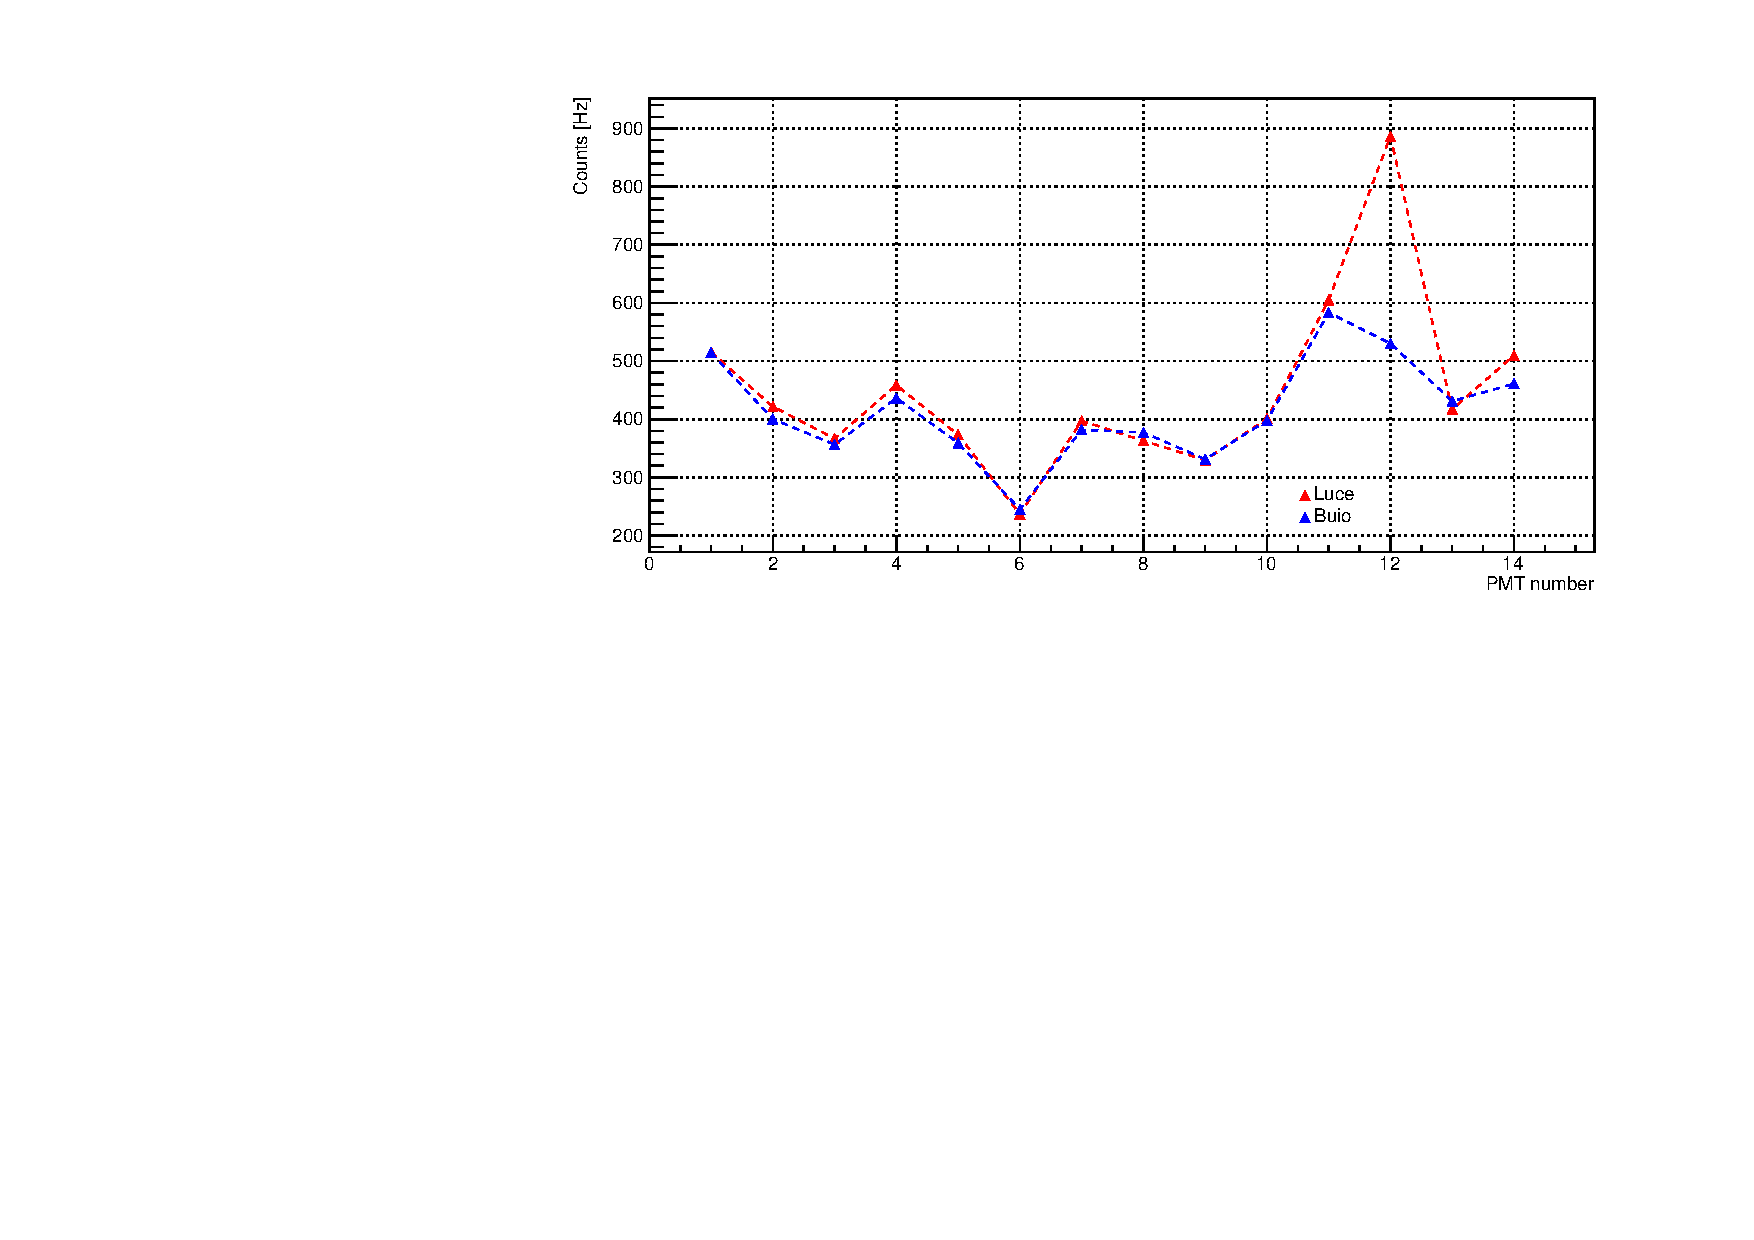
\includegraphics[scale=0.6]{img/luce_buio_100s.pdf}
	\caption{Situazione alla prima presa dati: è evidente la presenza di qualche difetto  nell'involucro della \emph{slab} a ridosso del fotomoltiplicatore nr.~12 che permette l'ingresso della radiazione ambientale.}
\end{figure}
%
\subsection{Studio dell'efficienza dei fotomoltiplicatori}
Lo scopo di questa fase consiste nella determinazione dell'efficienza dei 14 fotomoltiplicatori presenti nell'apparato sperimentale. Il comportamento di un generico fotomoltiplicatore, infatti, dipende dalla tensione a cui lo stesso è alimentato: al crescere della tensione, l'efficienza di rivelazione aumenta sino a saturare ad un valore massimo, raggiungendo dunque il regime di \textit{plateau} rispetto ad un contatore di riferimento.
Una volta individuato in quale intervallo di tensioni ciascun fototubo satura, il \emph{set-up} sperimentale ottimale prevede che ciascuno di essi venga alimentato al valore minimo possibile della tensione. 
La condizione di \textit{plateau} è importante per assicurare la massima efficienza di rivelazione possibile; una volta raggiunta, un aumento della tensione di alimentazione coincide solamente con un incremento di rumore.  

L'efficienza di rivelazione corrisponde alla quantità
\[\varepsilon = \frac{T\wedge PMT}{T}\;,\]
dove $T$ corrisponde al numero di eventi rivelati dal cosiddetto \textit{telescopio}, o \textit{trigger}, mentre $T\wedge PMT$ corrisponde alla quantità di eventi rivelati dal fototubo in esame in coincidenza con il telescopio. Il \emph{trigger} prevede l'utilizzo di due \emph{slab} esterne \linebreak ($G$ = grande, $P$ = piccola) poste in coincidenza di volta in volta con alcuni fototubi dell'apparato, differenti da quello momentaneamente esaminato. 

La disposizione del telescopio influenza notevolmente il numero di eventi $T$ tramite i quali si calcola l'efficienza dei diversi fotomoltiplicatori. Ai fini dell'esperimento, l'unica efficienza interessante è relativa alla rivelazione dei raggi cosmici tramite i consueti processi di eccitazione degli atomi del materiale plastico delle \emph{slab}. 
Tuttavia, questa procedura è stata disturbata dalla presenza delle guide di luce di raccordo tra un capo della \emph{slab} e il relativo fototubo: 
avendo a disposizione solo 2 \emph{slab} per formare il telescopio, nel conteggio di trigger entrano, per questioni geometriche, anche quei muoni che attraversano una guida di luce e non le sole \emph{slab}.

In virtù di queste considerazioni, i tracciatori esterni $G$ e $P$ sono stati posizionati sempre parallelamente alle \emph{slab} relative ai PMT esaminati\footnote{$G$ sopra la prima slab, $P$ appoggiata a terra.}: la rivelazione di eventi estranei  
a quelli di interesse \footnote{cioè non passanti per ambo le \emph{slab} ma attraverso una guida di luce} 
non modifica l'andamento della curva di efficienza, ma solamente i valori assunti dalla stessa, permettendo comunque di individuare il raggiungimento del regime di \emph{plateau}.

In base al PMT studiato, il telescopio corrisponde ad una delle seguenti configurazioni:
%%%%%%%%%%%%%%%%%%
\begin{itemize}
	\item \textbf{configurazione 1}: per lo studio dei PMT numero 1, 2, 5, 6, 7, 8, 9 e 10 i tracciatori $G$ e $P$ sono messi in coincidenza con i PMT numero 3 e 4 (relativi alla \emph{slab} più bassa), cioè \[T = G\wedge P \wedge PMT3 \wedge PMT4 \ ;\]
%
	\item \textbf{configurazione 2}: per lo studio dei PMT numero 3 e 4 i tracciatori $G$ e $P$ sono messi in coincidenza con i PMT numero 1, 2, 5, 6, cioè \[T = G\wedge P \wedge PMT1 \wedge PMT2 \wedge PMT5 \wedge PMT6 \ ; \]
%
	\item \textbf{configurazione 3}: le \emph{slab} laterali sono state momentaneamente tolte dalla loro posizione originale per essere appoggiate, sovrapposte nella stessa direzione e alternate in verso, su sgabelli di eguale altezza. In questo modo, per lo studio dei PMT 11 e 12, posizionati nello stesso verso, i tracciatori $G$, appoggiato sopra la prima delle quattro slab, e $P$, appoggiato a terra, sono stati messi in coincidenza con i PMT numero 13 e 14, anch'essi orientati nello stesso verso, opposto ai precedenti. In questo caso: \[T = G\wedge P \wedge PMT13 \wedge PMT14 \ ;\]
%
	\item \textbf{configurazione 4}: questa configurazione coincide con la numero 3, a patto di invertire i ruoli dei PMT 11 e 12 con quelli dei PMT 13 e 14. 
\end{itemize}
%%%%%%%%%%%%%%%%%%%
In appendice sono riportati i grafici relativi allo studio di tutti i 14 fotomoltiplicatori, sia per quanto riguarda la stima delle efficienze da vicino e da lontano, sia per quanto riguarda i conteggi da vicino.

L'efficienza di rivelazione è definita come segue:
$$\epsilon=\frac{T\wedge PMT}{T}$$
Al numero di eventi in coincidenza $T\wedge PMT$ è assegnata un'incertezza seguente la distribuzione binomiale, di cui si conosce la formula della varianza.  
Si ha allora che 
\[\sigma_{T\wedge PMT} = \sqrt{T \cdot \varepsilon \cdot  (1-\varepsilon)}\]
dove si è assunta come probabilità dell'evento favorevole il valore sperimentale dell'efficienza stessa $\varepsilon$.
L'errore sull'efficienza è dunque:
$$\sigma_\epsilon=\sqrt{ \left(\frac{\partial\epsilon}{\partial (T\wedge PMT)}\sigma_{T\wedge PMT}\right)^2 + \left(\frac{\partial \epsilon}{\partial T}\sigma_T\right)^2 }=\sqrt{\frac{\epsilon}{T}}$$
dove $\sigma_T = \sqrt{T}$.

%
\subsection{Misure di differenze temporali}\label{tac}
L'acquisizione della curva di decadimento dei muoni necessita di una procedura per la misura di intervalli temporali tramite un modulo Time to Amplitude Converter (TAC) e un modulo Analog to Digital Converter (ADC) per la conversione digitale. Le proprietà desiderate della catena elettronica devono essere opportunamente verificate prima di eseguire una procedura di calibrazione che permetta di associare un canale del multicanale ad un ben preciso valore temporale.

Inizialmente si è verificato il corretto comportamento della catena TAC + ADC rispetto a una distribuzione uniforme di ritardi temporali, ovvero generando due treni di segnali scorrelati da mandare in input alle entrate di START e STOP del TAC; ci si aspetta dalla raccolta di un numero statisticamente rilevante di dati una distribuzione perfettamente piatta. Per l'esperimento si è scelto di utilizzare il TAC nr.~437: in figura \ref{rumore1} è possibile osservare i risultati di una prima acquisizione.
%
\begin{figure}[h]
  \centering  
  \begin{adjustbox}{width=10cm}
    \begin{tikzpicture}
\pgfdeclareplotmark{cross} {
\pgfpathmoveto{\pgfpoint{-0.3\pgfplotmarksize}{\pgfplotmarksize}}
\pgfpathlineto{\pgfpoint{+0.3\pgfplotmarksize}{\pgfplotmarksize}}
\pgfpathlineto{\pgfpoint{+0.3\pgfplotmarksize}{0.3\pgfplotmarksize}}
\pgfpathlineto{\pgfpoint{+1\pgfplotmarksize}{0.3\pgfplotmarksize}}
\pgfpathlineto{\pgfpoint{+1\pgfplotmarksize}{-0.3\pgfplotmarksize}}
\pgfpathlineto{\pgfpoint{+0.3\pgfplotmarksize}{-0.3\pgfplotmarksize}}
\pgfpathlineto{\pgfpoint{+0.3\pgfplotmarksize}{-1.\pgfplotmarksize}}
\pgfpathlineto{\pgfpoint{-0.3\pgfplotmarksize}{-1.\pgfplotmarksize}}
\pgfpathlineto{\pgfpoint{-0.3\pgfplotmarksize}{-0.3\pgfplotmarksize}}
\pgfpathlineto{\pgfpoint{-1.\pgfplotmarksize}{-0.3\pgfplotmarksize}}
\pgfpathlineto{\pgfpoint{-1.\pgfplotmarksize}{0.3\pgfplotmarksize}}
\pgfpathlineto{\pgfpoint{-0.3\pgfplotmarksize}{0.3\pgfplotmarksize}}
\pgfpathclose
\pgfusepathqstroke
}
\pgfdeclareplotmark{cross*} {
\pgfpathmoveto{\pgfpoint{-0.3\pgfplotmarksize}{\pgfplotmarksize}}
\pgfpathlineto{\pgfpoint{+0.3\pgfplotmarksize}{\pgfplotmarksize}}
\pgfpathlineto{\pgfpoint{+0.3\pgfplotmarksize}{0.3\pgfplotmarksize}}
\pgfpathlineto{\pgfpoint{+1\pgfplotmarksize}{0.3\pgfplotmarksize}}
\pgfpathlineto{\pgfpoint{+1\pgfplotmarksize}{-0.3\pgfplotmarksize}}
\pgfpathlineto{\pgfpoint{+0.3\pgfplotmarksize}{-0.3\pgfplotmarksize}}
\pgfpathlineto{\pgfpoint{+0.3\pgfplotmarksize}{-1.\pgfplotmarksize}}
\pgfpathlineto{\pgfpoint{-0.3\pgfplotmarksize}{-1.\pgfplotmarksize}}
\pgfpathlineto{\pgfpoint{-0.3\pgfplotmarksize}{-0.3\pgfplotmarksize}}
\pgfpathlineto{\pgfpoint{-1.\pgfplotmarksize}{-0.3\pgfplotmarksize}}
\pgfpathlineto{\pgfpoint{-1.\pgfplotmarksize}{0.3\pgfplotmarksize}}
\pgfpathlineto{\pgfpoint{-0.3\pgfplotmarksize}{0.3\pgfplotmarksize}}
\pgfpathclose
\pgfusepathqfillstroke
}
\pgfdeclareplotmark{newstar} {
\pgfpathmoveto{\pgfqpoint{0pt}{\pgfplotmarksize}}
\pgfpathlineto{\pgfqpointpolar{44}{0.5\pgfplotmarksize}}
\pgfpathlineto{\pgfqpointpolar{18}{\pgfplotmarksize}}
\pgfpathlineto{\pgfqpointpolar{-20}{0.5\pgfplotmarksize}}
\pgfpathlineto{\pgfqpointpolar{-54}{\pgfplotmarksize}}
\pgfpathlineto{\pgfqpointpolar{-90}{0.5\pgfplotmarksize}}
\pgfpathlineto{\pgfqpointpolar{234}{\pgfplotmarksize}}
\pgfpathlineto{\pgfqpointpolar{198}{0.5\pgfplotmarksize}}
\pgfpathlineto{\pgfqpointpolar{162}{\pgfplotmarksize}}
\pgfpathlineto{\pgfqpointpolar{134}{0.5\pgfplotmarksize}}
\pgfpathclose
\pgfusepathqstroke
}
\pgfdeclareplotmark{newstar*} {
\pgfpathmoveto{\pgfqpoint{0pt}{\pgfplotmarksize}}
\pgfpathlineto{\pgfqpointpolar{44}{0.5\pgfplotmarksize}}
\pgfpathlineto{\pgfqpointpolar{18}{\pgfplotmarksize}}
\pgfpathlineto{\pgfqpointpolar{-20}{0.5\pgfplotmarksize}}
\pgfpathlineto{\pgfqpointpolar{-54}{\pgfplotmarksize}}
\pgfpathlineto{\pgfqpointpolar{-90}{0.5\pgfplotmarksize}}
\pgfpathlineto{\pgfqpointpolar{234}{\pgfplotmarksize}}
\pgfpathlineto{\pgfqpointpolar{198}{0.5\pgfplotmarksize}}
\pgfpathlineto{\pgfqpointpolar{162}{\pgfplotmarksize}}
\pgfpathlineto{\pgfqpointpolar{134}{0.5\pgfplotmarksize}}
\pgfpathclose
\pgfusepathqfillstroke
}
\definecolor{c}{rgb}{1,1,1};
\draw [color=c, fill=c] (0,0) rectangle (20,13.6103);
\draw [color=c, fill=c] (2.32092,1.37536) rectangle (17.765,12.2063);
\definecolor{c}{rgb}{0,0,0};
\draw [c,line width=0.9] (2.32092,1.37536) -- (2.32092,12.2063) -- (17.765,12.2063) -- (17.765,1.37536) -- (2.32092,1.37536);
\definecolor{c}{rgb}{1,1,1};
\draw [color=c, fill=c] (2.32092,1.37536) rectangle (17.765,12.2063);
\definecolor{c}{rgb}{0,0,0};
\draw [c,line width=0.9] (2.32092,1.37536) -- (2.32092,12.2063) -- (17.765,12.2063) -- (17.765,1.37536) -- (2.32092,1.37536);
\draw [c,line width=0.9] (2.32092,1.37536) -- (17.765,1.37536);
\draw [c,dash pattern=on 0.80pt off 1.60pt ,line width=0.9] (2.32092,12.2063) -- (2.32092,1.37536);
\draw [c,dash pattern=on 0.80pt off 1.60pt ,line width=0.9] (4.20619,12.2063) -- (4.20619,1.37536);
\draw [c,dash pattern=on 0.80pt off 1.60pt ,line width=0.9] (6.09146,12.2063) -- (6.09146,1.37536);
\draw [c,dash pattern=on 0.80pt off 1.60pt ,line width=0.9] (7.97672,12.2063) -- (7.97672,1.37536);
\draw [c,dash pattern=on 0.80pt off 1.60pt ,line width=0.9] (9.86199,12.2063) -- (9.86199,1.37536);
\draw [c,dash pattern=on 0.80pt off 1.60pt ,line width=0.9] (11.7473,12.2063) -- (11.7473,1.37536);
\draw [c,dash pattern=on 0.80pt off 1.60pt ,line width=0.9] (13.6325,12.2063) -- (13.6325,1.37536);
\draw [c,dash pattern=on 0.80pt off 1.60pt ,line width=0.9] (15.5178,12.2063) -- (15.5178,1.37536);
\draw [c,dash pattern=on 0.80pt off 1.60pt ,line width=0.9] (17.4031,12.2063) -- (17.4031,1.37536);
\draw [c,dash pattern=on 0.80pt off 1.60pt ,line width=0.9] (17.4031,12.2063) -- (17.4031,1.37536);
\draw [c,line width=0.9] (2.32092,1.37536) -- (2.32092,12.2063);
\draw [c,dash pattern=on 0.80pt off 1.60pt ,line width=0.9] (17.765,1.37536) -- (2.32092,1.37536);
\draw [c,dash pattern=on 0.80pt off 1.60pt ,line width=0.9] (17.765,3.18052) -- (2.32092,3.18052);
\draw [c,dash pattern=on 0.80pt off 1.60pt ,line width=0.9] (17.765,4.98567) -- (2.32092,4.98567);
\draw [c,dash pattern=on 0.80pt off 1.60pt ,line width=0.9] (17.765,6.79083) -- (2.32092,6.79083);
\draw [c,dash pattern=on 0.80pt off 1.60pt ,line width=0.9] (17.765,8.59599) -- (2.32092,8.59599);
\draw [c,dash pattern=on 0.80pt off 1.60pt ,line width=0.9] (17.765,10.4011) -- (2.32092,10.4011);
\draw [c,dash pattern=on 0.80pt off 1.60pt ,line width=0.9] (17.765,12.2063) -- (2.32092,12.2063);
\definecolor{c}{rgb}{0,0,1};
\draw [c,line width=0.9] (2.32092,1.37536) -- (2.35108,1.37536) -- (2.35108,1.37536) -- (2.38125,1.37536) -- (2.38125,1.37536) -- (2.41141,1.37536) -- (2.41141,1.37536) -- (2.44157,1.37536) -- (2.44157,1.37536) -- (2.47174,1.37536) --
 (2.47174,1.37536) -- (2.5019,1.37536) -- (2.5019,1.37536) -- (2.53207,1.37536) -- (2.53207,1.37536) -- (2.56223,1.37536) -- (2.56223,1.37536) -- (2.5924,1.37536) -- (2.5924,1.37536) -- (2.62256,1.37536) -- (2.62256,1.37536) -- (2.65272,1.37536) --
 (2.65272,1.37536) -- (2.68289,1.37536) -- (2.68289,1.37536) -- (2.71305,1.37536) -- (2.71305,1.37536) -- (2.74322,1.37536) -- (2.74322,1.37536) -- (2.77338,1.37536) -- (2.77338,1.37536) -- (2.80355,1.37536) -- (2.80355,1.37536) -- (2.83371,1.37536)
 -- (2.83371,1.37536) -- (2.86387,1.37536) -- (2.86387,12.2063) -- (2.89404,12.2063) -- (2.89404,12.2063) -- (2.9242,12.2063) -- (2.9242,7.0941) -- (2.95437,7.0941) -- (2.95437,7.06522) -- (2.98453,7.06522) -- (2.98453,7.07063) -- (3.0147,7.07063) --
 (3.0147,6.95149) -- (3.04486,6.95149) -- (3.04486,7.12659) -- (3.07502,7.12659) -- (3.07502,7.09229) -- (3.10519,7.09229) -- (3.10519,7.09951) -- (3.13535,7.09951) -- (3.13535,7.08327) -- (3.16552,7.08327) -- (3.16552,7.14825) -- (3.19568,7.14825)
 -- (3.19568,6.9208) -- (3.22585,6.9208) -- (3.22585,6.9894) -- (3.25601,6.9894) -- (3.25601,7.20241) -- (3.28617,7.20241) -- (3.28617,6.97315) -- (3.31634,6.97315) -- (3.31634,7.05799) -- (3.3465,7.05799) -- (3.3465,6.89553) -- (3.37667,6.89553) --
 (3.37667,6.92441) -- (3.40683,6.92441) -- (3.40683,7.20963) -- (3.437,7.20963) -- (3.437,7.10312) -- (3.46716,7.10312) -- (3.46716,6.93885) -- (3.49732,6.93885) -- (3.49732,7.21865) -- (3.52749,7.21865) -- (3.52749,7.24393) -- (3.55765,7.24393) --
 (3.55765,7.07966) -- (3.58782,7.07966) -- (3.58782,7.23129) -- (3.61798,7.23129) -- (3.61798,6.93344) -- (3.64815,6.93344) -- (3.64815,6.99662) -- (3.67831,6.99662) -- (3.67831,6.8847) -- (3.70848,6.8847) -- (3.70848,6.99662) -- (3.73864,6.99662) --
 (3.73864,7.07605) -- (3.7688,7.07605) -- (3.7688,6.92802) -- (3.79897,6.92802) -- (3.79897,7.11034) -- (3.82913,7.11034) -- (3.82913,6.90817) -- (3.8593,6.90817) -- (3.8593,6.79083) -- (3.88946,6.79083) -- (3.88946,6.86123) -- (3.91963,6.86123) --
 (3.91963,6.94788) -- (3.94979,6.94788) -- (3.94979,7.00203) -- (3.97995,7.00203) -- (3.97995,6.97676) -- (4.01012,6.97676) -- (4.01012,7.14825) -- (4.04028,7.14825) -- (4.04028,7.03633) -- (4.07045,7.03633) -- (4.07045,7.08146) -- (4.10061,7.08146)
 -- (4.10061,7.24573) -- (4.13078,7.24573) -- (4.13078,7.03814) -- (4.16094,7.03814) -- (4.16094,6.96954) -- (4.1911,6.96954) -- (4.1911,6.9551) -- (4.22127,6.9551) -- (4.22127,6.82152) -- (4.25143,6.82152) -- (4.25143,6.98759) -- (4.2816,6.98759) --
 (4.2816,6.95871) -- (4.31176,6.95871) -- (4.31176,7.1663) -- (4.34193,7.1663) -- (4.34193,7.03453) -- (4.37209,7.03453) -- (4.37209,7.07785) -- (4.40225,7.07785) -- (4.40225,7.06702) -- (4.43242,7.06702) -- (4.43242,6.8486) -- (4.46258,6.8486) --
 (4.46258,7.06883) -- (4.49275,7.06883) -- (4.49275,7.10854) -- (4.52291,7.10854) -- (4.52291,7.19338) -- (4.55308,7.19338) -- (4.55308,6.84499) -- (4.58324,6.84499) -- (4.58324,7.09049) -- (4.6134,7.09049) -- (4.6134,7.02189) -- (4.64357,7.02189) --
 (4.64357,6.94427) -- (4.67373,6.94427) -- (4.67373,6.9208) -- (4.7039,6.9208) -- (4.7039,7.01828) -- (4.73406,7.01828) -- (4.73406,6.77819) -- (4.76423,6.77819) -- (4.76423,7.16991) -- (4.79439,7.16991) -- (4.79439,6.90636) -- (4.82455,6.90636) --
 (4.82455,7.00925) -- (4.85472,7.00925) -- (4.85472,7.00564) -- (4.88488,7.00564) -- (4.88488,7.05799) -- (4.91505,7.05799) -- (4.91505,7.03092) -- (4.94521,7.03092) -- (4.94521,6.94246) -- (4.97538,6.94246) -- (4.97538,7.14284) -- (5.00554,7.14284)
 -- (5.00554,7.11215) -- (5.0357,7.11215) -- (5.0357,6.92983) -- (5.06587,6.92983) -- (5.06587,7.19699) -- (5.09603,7.19699) -- (5.09603,7.13562) -- (5.1262,7.13562) -- (5.1262,7.14645) -- (5.15636,7.14645) -- (5.15636,7.07424) -- (5.18653,7.07424)
 -- (5.18653,7.11576) -- (5.21669,7.11576) -- (5.21669,7.07785) -- (5.24685,7.07785) -- (5.24685,7.26198) -- (5.27702,7.26198) -- (5.27702,6.91358) -- (5.30718,6.91358) -- (5.30718,7.07424) -- (5.33735,7.07424) -- (5.33735,7.17533) --
 (5.36751,7.17533) -- (5.36751,7.07063) -- (5.39768,7.07063) -- (5.39768,6.97315) -- (5.42784,6.97315) -- (5.42784,7.0237) -- (5.458,7.0237) -- (5.458,7.00023) -- (5.48817,7.00023) -- (5.48817,6.76917) -- (5.51833,6.76917) -- (5.51833,7.00384) --
 (5.5485,7.00384) -- (5.5485,6.91719) -- (5.57866,6.91719) -- (5.57866,7.06883) -- (5.60883,7.06883) -- (5.60883,7.0598) -- (5.63899,7.0598) -- (5.63899,6.96593) -- (5.66916,6.96593) -- (5.66916,6.91539) -- (5.69932,6.91539) -- (5.69932,7.03272) --
 (5.72948,7.03272) -- (5.72948,7.14284) -- (5.75965,7.14284) -- (5.75965,7.17713) -- (5.78981,7.17713) -- (5.78981,6.91358) -- (5.81998,6.91358) -- (5.81998,7.06702) -- (5.85014,7.06702) -- (5.85014,7.07785) -- (5.88031,7.07785) -- (5.88031,6.89914)
 -- (5.91047,6.89914) -- (5.91047,7.05619) -- (5.94063,7.05619) -- (5.94063,6.83235) -- (5.9708,6.83235) -- (5.9708,7.22407) -- (6.00096,7.22407) -- (6.00096,7.09771) -- (6.03113,7.09771) -- (6.03113,6.98759) -- (6.06129,6.98759) -- (6.06129,7.05438)
 -- (6.09146,7.05438) -- (6.09146,6.93524) -- (6.12162,6.93524) -- (6.12162,7.04716) -- (6.15178,7.04716) -- (6.15178,6.96774) -- (6.18195,6.96774) -- (6.18195,7.08146) -- (6.21211,7.08146) -- (6.21211,7.0959) -- (6.24228,7.0959) -- (6.24228,7.1302)
 -- (6.27244,7.1302) -- (6.27244,7.09771) -- (6.30261,7.09771) -- (6.30261,6.80347) -- (6.33277,6.80347) -- (6.33277,7.19519) -- (6.36293,7.19519) -- (6.36293,7.12298) -- (6.3931,7.12298) -- (6.3931,6.97135) -- (6.42326,6.97135) -- (6.42326,7.03092)
 -- (6.45343,7.03092) -- (6.45343,7.02911) -- (6.48359,7.02911) -- (6.48359,6.9894) -- (6.51376,6.9894) -- (6.51376,7.16991) -- (6.54392,7.16991) -- (6.54392,6.9912) -- (6.57408,6.9912) -- (6.57408,6.92261) -- (6.60425,6.92261) -- (6.60425,6.92622)
 -- (6.63441,6.92622) -- (6.63441,7.1302) -- (6.66458,7.1302) -- (6.66458,6.9894) -- (6.69474,6.9894) -- (6.69474,7.05258) -- (6.72491,7.05258) -- (6.72491,6.94788) -- (6.75507,6.94788) -- (6.75507,7.02731) -- (6.78523,7.02731) -- (6.78523,7.11937)
 -- (6.8154,7.11937) -- (6.8154,7.00203) -- (6.84556,7.00203) -- (6.84556,7.08868) -- (6.87573,7.08868) -- (6.87573,7.01648) -- (6.90589,7.01648) -- (6.90589,6.92441) -- (6.93606,6.92441) -- (6.93606,6.99842) -- (6.96622,6.99842) -- (6.96622,7.05619)
 -- (6.99638,7.05619) -- (6.99638,6.97857) -- (7.02655,6.97857) -- (7.02655,7.03453) -- (7.05671,7.03453) -- (7.05671,7.12117) -- (7.08688,7.12117) -- (7.08688,7.02189) -- (7.11704,7.02189) -- (7.11704,7.07244) -- (7.14721,7.07244) --
 (7.14721,6.98037) -- (7.17737,6.98037) -- (7.17737,7.18977) -- (7.20753,7.18977) -- (7.20753,6.9912) -- (7.2377,6.9912) -- (7.2377,6.99301) -- (7.26786,6.99301) -- (7.26786,7.04716) -- (7.29803,7.04716) -- (7.29803,7.03994) -- (7.32819,7.03994) --
 (7.32819,7.02731) -- (7.35836,7.02731) -- (7.35836,6.83957) -- (7.38852,6.83957) -- (7.38852,7.00203) -- (7.41868,7.00203) -- (7.41868,7.01467) -- (7.44885,7.01467) -- (7.44885,7.04536) -- (7.47901,7.04536) -- (7.47901,7.03092) -- (7.50918,7.03092)
 -- (7.50918,6.92622) -- (7.53934,6.92622) -- (7.53934,7.09771) -- (7.56951,7.09771) -- (7.56951,6.9894) -- (7.59967,6.9894) -- (7.59967,6.81249) -- (7.62984,6.81249) -- (7.62984,7.08327) -- (7.66,7.08327) -- (7.66,7.08507) -- (7.69016,7.08507) --
 (7.69016,7.25295) -- (7.72033,7.25295) -- (7.72033,6.98579) -- (7.75049,6.98579) -- (7.75049,6.98218) -- (7.78066,6.98218) -- (7.78066,6.92622) -- (7.81082,6.92622) -- (7.81082,6.83777) -- (7.84099,6.83777) -- (7.84099,7.02009) -- (7.87115,7.02009)
 -- (7.87115,6.98218) -- (7.90131,6.98218) -- (7.90131,6.8865) -- (7.93148,6.8865) -- (7.93148,7.04716) -- (7.96164,7.04716) -- (7.96164,7.20421) -- (7.99181,7.20421) -- (7.99181,6.99842) -- (8.02197,6.99842) -- (8.02197,7.12479) -- (8.05214,7.12479)
 -- (8.05214,7.15547) -- (8.0823,7.15547) -- (8.0823,7.12298) -- (8.11246,7.12298) -- (8.11246,6.99842) -- (8.14263,6.99842) -- (8.14263,6.94246) -- (8.17279,6.94246) -- (8.17279,7.04355) -- (8.20296,7.04355) -- (8.20296,7.10493) -- (8.23312,7.10493)
 -- (8.23312,7.10132) -- (8.26329,7.10132) -- (8.26329,7.11576) -- (8.29345,7.11576) -- (8.29345,6.87748) -- (8.32361,6.87748) -- (8.32361,7.11756) -- (8.35378,7.11756) -- (8.35378,7.10854) -- (8.38394,7.10854) -- (8.38394,7.21685) --
 (8.41411,7.21685) -- (8.41411,7.08688) -- (8.44427,7.08688) -- (8.44427,6.81971) -- (8.47444,6.81971) -- (8.47444,7.00564) -- (8.5046,7.00564) -- (8.5046,7.02731) -- (8.53476,7.02731) -- (8.53476,7.02911) -- (8.56493,7.02911) -- (8.56493,7.04536) --
 (8.59509,7.04536) -- (8.59509,7.03994) -- (8.62526,7.03994) -- (8.62526,6.94969) -- (8.65542,6.94969) -- (8.65542,7.1284) -- (8.68559,7.1284) -- (8.68559,6.97857) -- (8.71575,6.97857) -- (8.71575,7.14284) -- (8.74591,7.14284) -- (8.74591,6.96052) --
 (8.77608,6.96052) -- (8.77608,7.25837) -- (8.80624,7.25837) -- (8.80624,6.89734) -- (8.83641,6.89734) -- (8.83641,6.89553) -- (8.86657,6.89553) -- (8.86657,6.89192) -- (8.89674,6.89192) -- (8.89674,7.01828) -- (8.9269,7.01828) -- (8.9269,7.11034) --
 (8.95706,7.11034) -- (8.95706,7.1663) -- (8.98723,7.1663) -- (8.98723,6.94246) -- (9.01739,6.94246) -- (9.01739,6.89553) -- (9.04756,6.89553) -- (9.04756,7.08146) -- (9.07772,7.08146) -- (9.07772,6.97496) -- (9.10789,6.97496) -- (9.10789,7.17172) --
 (9.13805,7.17172) -- (9.13805,7.05799) -- (9.16821,7.05799) -- (9.16821,7.00564) -- (9.19838,7.00564) -- (9.19838,7.15186) -- (9.22854,7.15186) -- (9.22854,6.94607) -- (9.25871,6.94607) -- (9.25871,6.97857) -- (9.28887,6.97857) -- (9.28887,6.90095)
 -- (9.31904,6.90095) -- (9.31904,6.89914) -- (9.3492,6.89914) -- (9.3492,7.01287) -- (9.37936,7.01287) -- (9.37936,7.24212) -- (9.40953,7.24212) -- (9.40953,7.10493) -- (9.43969,7.10493) -- (9.43969,6.8865) -- (9.46986,6.8865) -- (9.46986,7.10132)
 -- (9.50002,7.10132) -- (9.50002,6.94788) -- (9.53019,6.94788) -- (9.53019,7.05438) -- (9.56035,7.05438) -- (9.56035,6.99301) -- (9.59052,6.99301) -- (9.59052,7.04536) -- (9.62068,7.04536) -- (9.62068,7.02009) -- (9.65084,7.02009) --
 (9.65084,7.00384) -- (9.68101,7.00384) -- (9.68101,7.16089) -- (9.71117,7.16089) -- (9.71117,6.96052) -- (9.74134,6.96052) -- (9.74134,7.12659) -- (9.7715,7.12659) -- (9.7715,7.01467) -- (9.80167,7.01467) -- (9.80167,6.96774) -- (9.83183,6.96774) --
 (9.83183,6.87928) -- (9.86199,6.87928) -- (9.86199,6.87387) -- (9.89216,6.87387) -- (9.89216,7.0616) -- (9.92232,7.0616) -- (9.92232,7.10493) -- (9.95249,7.10493) -- (9.95249,7.10312) -- (9.98265,7.10312) -- (9.98265,6.97857) -- (10.0128,6.97857) --
 (10.0128,7.17352) -- (10.043,7.17352) -- (10.043,7.13923) -- (10.0731,7.13923) -- (10.0731,6.99481) -- (10.1033,6.99481) -- (10.1033,7.21324) -- (10.1335,7.21324) -- (10.1335,7.19338) -- (10.1636,7.19338) -- (10.1636,6.90636) -- (10.1938,6.90636) --
 (10.1938,7.04355) -- (10.224,7.04355) -- (10.224,6.99481) -- (10.2541,6.99481) -- (10.2541,6.9912) -- (10.2843,6.9912) -- (10.2843,7.01828) -- (10.3145,7.01828) -- (10.3145,7.05619) -- (10.3446,7.05619) -- (10.3446,6.99301) -- (10.3748,6.99301) --
 (10.3748,7.18616) -- (10.405,7.18616) -- (10.405,6.9551) -- (10.4351,6.9551) -- (10.4351,7.13201) -- (10.4653,7.13201) -- (10.4653,7.08327) -- (10.4954,7.08327) -- (10.4954,6.86304) -- (10.5256,6.86304) -- (10.5256,6.89192) -- (10.5558,6.89192) --
 (10.5558,6.99662) -- (10.5859,6.99662) -- (10.5859,6.93524) -- (10.6161,6.93524) -- (10.6161,7.21143) -- (10.6463,7.21143) -- (10.6463,7.00203) -- (10.6764,7.00203) -- (10.6764,7.09049) -- (10.7066,7.09049) -- (10.7066,7.12479) -- (10.7368,7.12479)
 -- (10.7368,6.76917) -- (10.7669,6.76917) -- (10.7669,7.20602) -- (10.7971,7.20602) -- (10.7971,6.88109) -- (10.8273,6.88109) -- (10.8273,6.73126) -- (10.8574,6.73126) -- (10.8574,7.0959) -- (10.8876,7.0959) -- (10.8876,6.93163) -- (10.9177,6.93163)
 -- (10.9177,6.94607) -- (10.9479,6.94607) -- (10.9479,7.271) -- (10.9781,7.271) -- (10.9781,7.36126) -- (11.0082,7.36126) -- (11.0082,7.36307) -- (11.0384,7.36307) -- (11.0384,7.66814) -- (11.0686,7.66814) -- (11.0686,7.81436) -- (11.0987,7.81436)
 -- (11.0987,8.05805) -- (11.1289,8.05805) -- (11.1289,8.14831) -- (11.1591,8.14831) -- (11.1591,7.9353) -- (11.1892,7.9353) -- (11.1892,7.78186) -- (11.2194,7.78186) -- (11.2194,7.62301) -- (11.2496,7.62301) -- (11.2496,7.42625) -- (11.2797,7.42625)
 -- (11.2797,7.55983) -- (11.3099,7.55983) -- (11.3099,7.17533) -- (11.34,7.17533) -- (11.34,7.32516) -- (11.3702,7.32516) -- (11.3702,7.31613) -- (11.4004,7.31613) -- (11.4004,7.50387) -- (11.4305,7.50387) -- (11.4305,7.5165) -- (11.4607,7.5165) --
 (11.4607,7.29267) -- (11.4909,7.29267) -- (11.4909,7.47499) -- (11.521,7.47499) -- (11.521,7.38112) -- (11.5512,7.38112) -- (11.5512,7.56163) -- (11.5814,7.56163) -- (11.5814,7.30891) -- (11.6115,7.30891) -- (11.6115,7.51109) -- (11.6417,7.51109) --
 (11.6417,7.41181) -- (11.6719,7.41181) -- (11.6719,7.41181) -- (11.702,7.41181) -- (11.702,7.4082) -- (11.7322,7.4082) -- (11.7322,7.41722) -- (11.7623,7.41722) -- (11.7623,7.39556) -- (11.7925,7.39556) -- (11.7925,7.38473) -- (11.8227,7.38473) --
 (11.8227,7.43888) -- (11.8528,7.43888) -- (11.8528,7.271) -- (11.883,7.271) -- (11.883,7.39014) -- (11.9132,7.39014) -- (11.9132,7.21324) -- (11.9433,7.21324) -- (11.9433,7.31433) -- (11.9735,7.31433) -- (11.9735,7.33238) -- (12.0037,7.33238) --
 (12.0037,7.10673) -- (12.0338,7.10673) -- (12.0338,7.10132) -- (12.064,7.10132) -- (12.064,7.15728) -- (12.0942,7.15728) -- (12.0942,7.15547) -- (12.1243,7.15547) -- (12.1243,7.09229) -- (12.1545,7.09229) -- (12.1545,7.17172) -- (12.1846,7.17172) --
 (12.1846,6.95149) -- (12.2148,6.95149) -- (12.2148,7.08146) -- (12.245,7.08146) -- (12.245,7.00564) -- (12.2751,7.00564) -- (12.2751,7.03272) -- (12.3053,7.03272) -- (12.3053,7.01828) -- (12.3355,7.01828) -- (12.3355,6.87387) -- (12.3656,6.87387) --
 (12.3656,6.87387) -- (12.3958,6.87387) -- (12.3958,6.8504) -- (12.426,6.8504) -- (12.426,6.9208) -- (12.4561,6.9208) -- (12.4561,6.91358) -- (12.4863,6.91358) -- (12.4863,6.96052) -- (12.5165,6.96052) -- (12.5165,7.07244) -- (12.5466,7.07244) --
 (12.5466,6.93344) -- (12.5768,6.93344) -- (12.5768,6.93885) -- (12.6069,6.93885) -- (12.6069,7.05438) -- (12.6371,7.05438) -- (12.6371,6.92802) -- (12.6673,6.92802) -- (12.6673,6.96593) -- (12.6974,6.96593) -- (12.6974,7.05258) -- (12.7276,7.05258)
 -- (12.7276,6.78181) -- (12.7578,6.78181) -- (12.7578,6.98398) -- (12.7879,6.98398) -- (12.7879,7.02189) -- (12.8181,7.02189) -- (12.8181,6.81249) -- (12.8483,6.81249) -- (12.8483,6.97676) -- (12.8784,6.97676) -- (12.8784,6.72404) --
 (12.9086,6.72404) -- (12.9086,6.94246) -- (12.9388,6.94246) -- (12.9388,7.03633) -- (12.9689,7.03633) -- (12.9689,6.89192) -- (12.9991,6.89192) -- (12.9991,6.85943) -- (13.0292,6.85943) -- (13.0292,6.83957) -- (13.0594,6.83957) -- (13.0594,6.96593)
 -- (13.0896,6.96593) -- (13.0896,6.98037) -- (13.1197,6.98037) -- (13.1197,7.05438) -- (13.1499,7.05438) -- (13.1499,6.66086) -- (13.1801,6.66086) -- (13.1801,6.77458) -- (13.2102,6.77458) -- (13.2102,6.8865) -- (13.2404,6.8865) -- (13.2404,6.93344)
 -- (13.2706,6.93344) -- (13.2706,6.90817) -- (13.3007,6.90817) -- (13.3007,6.95691) -- (13.3309,6.95691) -- (13.3309,7.18977) -- (13.3611,7.18977) -- (13.3611,6.90636) -- (13.3912,6.90636) -- (13.3912,6.9208) -- (13.4214,6.9208) -- (13.4214,6.79805)
 -- (13.4515,6.79805) -- (13.4515,6.84138) -- (13.4817,6.84138) -- (13.4817,6.97135) -- (13.5119,6.97135) -- (13.5119,6.96413) -- (13.542,6.96413) -- (13.542,6.89011) -- (13.5722,6.89011) -- (13.5722,7.09771) -- (13.6024,7.09771) -- (13.6024,6.91539)
 -- (13.6325,6.91539) -- (13.6325,6.85762) -- (13.6627,6.85762) -- (13.6627,6.87567) -- (13.6929,6.87567) -- (13.6929,7.01287) -- (13.723,7.01287) -- (13.723,7.00564) -- (13.7532,7.00564) -- (13.7532,6.78722) -- (13.7834,6.78722) -- (13.7834,6.85401)
 -- (13.8135,6.85401) -- (13.8135,6.77458) -- (13.8437,6.77458) -- (13.8437,6.89914) -- (13.8738,6.89914) -- (13.8738,7.43347) -- (13.904,7.43347) -- (13.904,7.12298) -- (13.9342,7.12298) -- (13.9342,7.07244) -- (13.9643,7.07244) -- (13.9643,7.00023)
 -- (13.9945,7.00023) -- (13.9945,6.99842) -- (14.0247,6.99842) -- (14.0247,7.07605) -- (14.0548,7.07605) -- (14.0548,6.94788) -- (14.085,6.94788) -- (14.085,6.96774) -- (14.1152,6.96774) -- (14.1152,7.11215) -- (14.1453,7.11215) -- (14.1453,6.97676)
 -- (14.1755,6.97676) -- (14.1755,7.09049) -- (14.2057,7.09049) -- (14.2057,6.95691) -- (14.2358,6.95691) -- (14.2358,6.9208) -- (14.266,6.9208) -- (14.266,6.89011) -- (14.2961,6.89011) -- (14.2961,6.99481) -- (14.3263,6.99481) -- (14.3263,6.97496)
 -- (14.3565,6.97496) -- (14.3565,6.91178) -- (14.3866,6.91178) -- (14.3866,7.03633) -- (14.4168,7.03633) -- (14.4168,7.19338) -- (14.447,7.19338) -- (14.447,6.84318) -- (14.4771,6.84318) -- (14.4771,7.15367) -- (14.5073,7.15367) -- (14.5073,6.91539)
 -- (14.5375,6.91539) -- (14.5375,6.9912) -- (14.5676,6.9912) -- (14.5676,7.16811) -- (14.5978,7.16811) -- (14.5978,6.94607) -- (14.628,6.94607) -- (14.628,7.0616) -- (14.6581,7.0616) -- (14.6581,7.05077) -- (14.6883,7.05077) -- (14.6883,6.919) --
 (14.7184,6.919) -- (14.7184,6.97135) -- (14.7486,6.97135) -- (14.7486,6.96232) -- (14.7788,6.96232) -- (14.7788,6.86845) -- (14.8089,6.86845) -- (14.8089,7.08507) -- (14.8391,7.08507) -- (14.8391,6.97135) -- (14.8693,6.97135) -- (14.8693,7.17894) --
 (14.8994,7.17894) -- (14.8994,7.00203) -- (14.9296,7.00203) -- (14.9296,7.28725) -- (14.9598,7.28725) -- (14.9598,6.94969) -- (14.9899,6.94969) -- (14.9899,7.09771) -- (15.0201,7.09771) -- (15.0201,6.95871) -- (15.0503,6.95871) -- (15.0503,6.84499)
 -- (15.0804,6.84499) -- (15.0804,7.06702) -- (15.1106,7.06702) -- (15.1106,6.93163) -- (15.1407,6.93163) -- (15.1407,6.97676) -- (15.1709,6.97676) -- (15.1709,6.8865) -- (15.2011,6.8865) -- (15.2011,7.11034) -- (15.2312,7.11034) -- (15.2312,7.13562)
 -- (15.2614,7.13562) -- (15.2614,7.00203) -- (15.2916,7.00203) -- (15.2916,7.05438) -- (15.3217,7.05438) -- (15.3217,7.13381) -- (15.3519,7.13381) -- (15.3519,7.07605) -- (15.3821,7.07605) -- (15.3821,7.04716) -- (15.4122,7.04716) --
 (15.4122,6.94066) -- (15.4424,6.94066) -- (15.4424,7.08507) -- (15.4726,7.08507) -- (15.4726,6.95871) -- (15.5027,6.95871) -- (15.5027,7.15547) -- (15.5329,7.15547) -- (15.5329,6.92622) -- (15.563,6.92622) -- (15.563,7.0959) -- (15.5932,7.0959) --
 (15.5932,7.00203) -- (15.6234,7.00203) -- (15.6234,6.97676) -- (15.6535,6.97676) -- (15.6535,6.85762) -- (15.6837,6.85762) -- (15.6837,6.79805) -- (15.7139,6.79805) -- (15.7139,6.99301) -- (15.744,6.99301) -- (15.744,7.05619) -- (15.7742,7.05619) --
 (15.7742,7.10312) -- (15.8044,7.10312) -- (15.8044,6.96232) -- (15.8345,6.96232) -- (15.8345,7.04897) -- (15.8647,7.04897) -- (15.8647,7.03633) -- (15.8949,7.03633) -- (15.8949,6.89192) -- (15.925,6.89192) -- (15.925,6.94427) -- (15.9552,6.94427) --
 (15.9552,7.04536) -- (15.9853,7.04536) -- (15.9853,7.08688) -- (16.0155,7.08688) -- (16.0155,7.08507) -- (16.0457,7.08507) -- (16.0457,7.00203) -- (16.0758,7.00203) -- (16.0758,7.05258) -- (16.106,7.05258) -- (16.106,6.95871) -- (16.1362,6.95871) --
 (16.1362,7.05258) -- (16.1663,7.05258) -- (16.1663,7.09229) -- (16.1965,7.09229) -- (16.1965,7.00745) -- (16.2267,7.00745) -- (16.2267,7.31072) -- (16.2568,7.31072) -- (16.2568,6.98579) -- (16.287,6.98579) -- (16.287,6.9551) -- (16.3172,6.9551) --
 (16.3172,7.01467) -- (16.3473,7.01467) -- (16.3473,7.10132) -- (16.3775,7.10132) -- (16.3775,6.9533) -- (16.4076,6.9533) -- (16.4076,7.19158) -- (16.4378,7.19158) -- (16.4378,7.07966) -- (16.468,7.07966) -- (16.468,7.06702) -- (16.4981,7.06702) --
 (16.4981,7.09049) -- (16.5283,7.09049) -- (16.5283,7.14103) -- (16.5585,7.14103) -- (16.5585,6.88831) -- (16.5886,6.88831) -- (16.5886,7.1302) -- (16.6188,7.1302) -- (16.6188,7.13201) -- (16.649,7.13201) -- (16.649,7.1663) -- (16.6791,7.1663) --
 (16.6791,7.0598) -- (16.7093,7.0598) -- (16.7093,7.03453) -- (16.7395,7.03453) -- (16.7395,6.94607) -- (16.7696,6.94607) -- (16.7696,6.92802) -- (16.7998,6.92802) -- (16.7998,6.97496) -- (16.83,6.97496) -- (16.83,7.20963) -- (16.8601,7.20963) --
 (16.8601,7.08327) -- (16.8903,7.08327) -- (16.8903,6.91358) -- (16.9204,6.91358) -- (16.9204,6.9912) -- (16.9506,6.9912) -- (16.9506,7.14103) -- (16.9808,7.14103) -- (16.9808,7.14464) -- (17.0109,7.14464) -- (17.0109,7.07785) -- (17.0411,7.07785) --
 (17.0411,7.07785) -- (17.0713,7.07785) -- (17.0713,6.97496) -- (17.1014,6.97496) -- (17.1014,7.10312) -- (17.1316,7.10312) -- (17.1316,6.99842) -- (17.1618,6.99842) -- (17.1618,7.08327) -- (17.1919,7.08327) -- (17.1919,6.98218) -- (17.2221,6.98218)
 -- (17.2221,7.08507) -- (17.2522,7.08507) -- (17.2522,6.92622) -- (17.2824,6.92622) -- (17.2824,7.13201) -- (17.3126,7.13201) -- (17.3126,7.03453) -- (17.3427,7.03453) -- (17.3427,7.0941) -- (17.3729,7.0941) -- (17.3729,6.99662) -- (17.4031,6.99662)
 -- (17.4031,7.09951) -- (17.4332,7.09951) -- (17.4332,7.1284) -- (17.4634,7.1284) -- (17.4634,7.17894) -- (17.4936,7.17894) -- (17.4936,7.07063) -- (17.5237,7.07063) -- (17.5237,7.03092) -- (17.5539,7.03092) -- (17.5539,6.74931) -- (17.5841,6.74931)
 -- (17.5841,3.88994) -- (17.6142,3.88994) -- (17.6142,1.37536) -- (17.6444,1.37536) -- (17.6444,1.37536) -- (17.6745,1.37536) -- (17.6745,1.37536) -- (17.7047,1.37536) -- (17.7047,1.37536) -- (17.7349,1.37536) -- (17.7349,1.37536) --
 (17.765,1.37536);
\definecolor{c}{rgb}{0,0,0};
\draw [c,line width=0.9] (2.32092,1.37536) -- (17.765,1.37536);
\draw [anchor= east] (17.765,0.395416) node[scale=1.52731, color=c, rotate=0]{Canale};
\draw [c,line width=0.9] (2.32092,1.69066) -- (2.32092,1.37536);
\draw [c,line width=0.9] (2.69797,1.53301) -- (2.69797,1.37536);
\draw [c,line width=0.9] (3.07502,1.53301) -- (3.07502,1.37536);
\draw [c,line width=0.9] (3.45208,1.53301) -- (3.45208,1.37536);
\draw [c,line width=0.9] (3.82913,1.53301) -- (3.82913,1.37536);
\draw [c,line width=0.9] (4.20619,1.69066) -- (4.20619,1.37536);
\draw [c,line width=0.9] (4.58324,1.53301) -- (4.58324,1.37536);
\draw [c,line width=0.9] (4.96029,1.53301) -- (4.96029,1.37536);
\draw [c,line width=0.9] (5.33735,1.53301) -- (5.33735,1.37536);
\draw [c,line width=0.9] (5.7144,1.53301) -- (5.7144,1.37536);
\draw [c,line width=0.9] (6.09146,1.69066) -- (6.09146,1.37536);
\draw [c,line width=0.9] (6.46851,1.53301) -- (6.46851,1.37536);
\draw [c,line width=0.9] (6.84556,1.53301) -- (6.84556,1.37536);
\draw [c,line width=0.9] (7.22262,1.53301) -- (7.22262,1.37536);
\draw [c,line width=0.9] (7.59967,1.53301) -- (7.59967,1.37536);
\draw [c,line width=0.9] (7.97672,1.69066) -- (7.97672,1.37536);
\draw [c,line width=0.9] (8.35378,1.53301) -- (8.35378,1.37536);
\draw [c,line width=0.9] (8.73083,1.53301) -- (8.73083,1.37536);
\draw [c,line width=0.9] (9.10789,1.53301) -- (9.10789,1.37536);
\draw [c,line width=0.9] (9.48494,1.53301) -- (9.48494,1.37536);
\draw [c,line width=0.9] (9.86199,1.69066) -- (9.86199,1.37536);
\draw [c,line width=0.9] (10.239,1.53301) -- (10.239,1.37536);
\draw [c,line width=0.9] (10.6161,1.53301) -- (10.6161,1.37536);
\draw [c,line width=0.9] (10.9932,1.53301) -- (10.9932,1.37536);
\draw [c,line width=0.9] (11.3702,1.53301) -- (11.3702,1.37536);
\draw [c,line width=0.9] (11.7473,1.69066) -- (11.7473,1.37536);
\draw [c,line width=0.9] (12.1243,1.53301) -- (12.1243,1.37536);
\draw [c,line width=0.9] (12.5014,1.53301) -- (12.5014,1.37536);
\draw [c,line width=0.9] (12.8784,1.53301) -- (12.8784,1.37536);
\draw [c,line width=0.9] (13.2555,1.53301) -- (13.2555,1.37536);
\draw [c,line width=0.9] (13.6325,1.69066) -- (13.6325,1.37536);
\draw [c,line width=0.9] (14.0096,1.53301) -- (14.0096,1.37536);
\draw [c,line width=0.9] (14.3866,1.53301) -- (14.3866,1.37536);
\draw [c,line width=0.9] (14.7637,1.53301) -- (14.7637,1.37536);
\draw [c,line width=0.9] (15.1407,1.53301) -- (15.1407,1.37536);
\draw [c,line width=0.9] (15.5178,1.69066) -- (15.5178,1.37536);
\draw [c,line width=0.9] (15.8949,1.53301) -- (15.8949,1.37536);
\draw [c,line width=0.9] (16.2719,1.53301) -- (16.2719,1.37536);
\draw [c,line width=0.9] (16.649,1.53301) -- (16.649,1.37536);
\draw [c,line width=0.9] (17.026,1.53301) -- (17.026,1.37536);
\draw [c,line width=0.9] (17.4031,1.69066) -- (17.4031,1.37536);
\draw [c,line width=0.9] (17.4031,1.69066) -- (17.4031,1.37536);
\draw [anchor=base] (2.32092,0.762894) node[scale=1.52731, color=c, rotate=0]{0};
\draw [anchor=base] (4.20619,0.762894) node[scale=1.52731, color=c, rotate=0]{500};
\draw [anchor=base] (6.09146,0.762894) node[scale=1.52731, color=c, rotate=0]{1000};
\draw [anchor=base] (7.97672,0.762894) node[scale=1.52731, color=c, rotate=0]{1500};
\draw [anchor=base] (9.86199,0.762894) node[scale=1.52731, color=c, rotate=0]{2000};
\draw [anchor=base] (11.7473,0.762894) node[scale=1.52731, color=c, rotate=0]{2500};
\draw [anchor=base] (13.6325,0.762894) node[scale=1.52731, color=c, rotate=0]{3000};
\draw [anchor=base] (15.5178,0.762894) node[scale=1.52731, color=c, rotate=0]{3500};
\draw [anchor=base] (17.4031,0.762894) node[scale=1.52731, color=c, rotate=0]{4000};
\draw [c,line width=0.9] (2.32092,1.37536) -- (2.32092,12.2063);
\draw [anchor= east] (0.496917,12.2063) node[scale=1.52731, color=c, rotate=90]{Conteggi};
\draw [c,line width=0.9] (2.79839,1.37536) -- (2.32092,1.37536);
\draw [c,line width=0.9] (2.55965,1.73639) -- (2.32092,1.73639);
\draw [c,line width=0.9] (2.55965,2.09742) -- (2.32092,2.09742);
\draw [c,line width=0.9] (2.55965,2.45845) -- (2.32092,2.45845);
\draw [c,line width=0.9] (2.55965,2.81948) -- (2.32092,2.81948);
\draw [c,line width=0.9] (2.79839,3.18052) -- (2.32092,3.18052);
\draw [c,line width=0.9] (2.55965,3.54155) -- (2.32092,3.54155);
\draw [c,line width=0.9] (2.55965,3.90258) -- (2.32092,3.90258);
\draw [c,line width=0.9] (2.55965,4.26361) -- (2.32092,4.26361);
\draw [c,line width=0.9] (2.55965,4.62464) -- (2.32092,4.62464);
\draw [c,line width=0.9] (2.79839,4.98567) -- (2.32092,4.98567);
\draw [c,line width=0.9] (2.55965,5.3467) -- (2.32092,5.3467);
\draw [c,line width=0.9] (2.55965,5.70774) -- (2.32092,5.70774);
\draw [c,line width=0.9] (2.55965,6.06877) -- (2.32092,6.06877);
\draw [c,line width=0.9] (2.55965,6.4298) -- (2.32092,6.4298);
\draw [c,line width=0.9] (2.79839,6.79083) -- (2.32092,6.79083);
\draw [c,line width=0.9] (2.55965,7.15186) -- (2.32092,7.15186);
\draw [c,line width=0.9] (2.55965,7.51289) -- (2.32092,7.51289);
\draw [c,line width=0.9] (2.55965,7.87393) -- (2.32092,7.87393);
\draw [c,line width=0.9] (2.55965,8.23496) -- (2.32092,8.23496);
\draw [c,line width=0.9] (2.79839,8.59599) -- (2.32092,8.59599);
\draw [c,line width=0.9] (2.55965,8.95702) -- (2.32092,8.95702);
\draw [c,line width=0.9] (2.55965,9.31805) -- (2.32092,9.31805);
\draw [c,line width=0.9] (2.55965,9.67908) -- (2.32092,9.67908);
\draw [c,line width=0.9] (2.55965,10.0401) -- (2.32092,10.0401);
\draw [c,line width=0.9] (2.79839,10.4011) -- (2.32092,10.4011);
\draw [c,line width=0.9] (2.55965,10.7622) -- (2.32092,10.7622);
\draw [c,line width=0.9] (2.55965,11.1232) -- (2.32092,11.1232);
\draw [c,line width=0.9] (2.55965,11.4842) -- (2.32092,11.4842);
\draw [c,line width=0.9] (2.55965,11.8453) -- (2.32092,11.8453);
\draw [c,line width=0.9] (2.79839,12.2063) -- (2.32092,12.2063);
\draw [anchor= east] (2.22092,1.37536) node[scale=1.52731, color=c, rotate=0]{0};
\draw [anchor= east] (2.22092,3.18052) node[scale=1.52731, color=c, rotate=0]{1000};
\draw [anchor= east] (2.22092,4.98567) node[scale=1.52731, color=c, rotate=0]{2000};
\draw [anchor= east] (2.22092,6.79083) node[scale=1.52731, color=c, rotate=0]{3000};
\draw [anchor= east] (2.22092,8.59599) node[scale=1.52731, color=c, rotate=0]{4000};
\draw [anchor= east] (2.22092,10.4011) node[scale=1.52731, color=c, rotate=0]{5000};
\draw [anchor= east] (2.22092,12.2063) node[scale=1.52731, color=c, rotate=0]{6000};
\draw (10,12.7937) node[scale=1.20912, color=c, rotate=0]{};
\end{tikzpicture}

  \end{adjustbox}%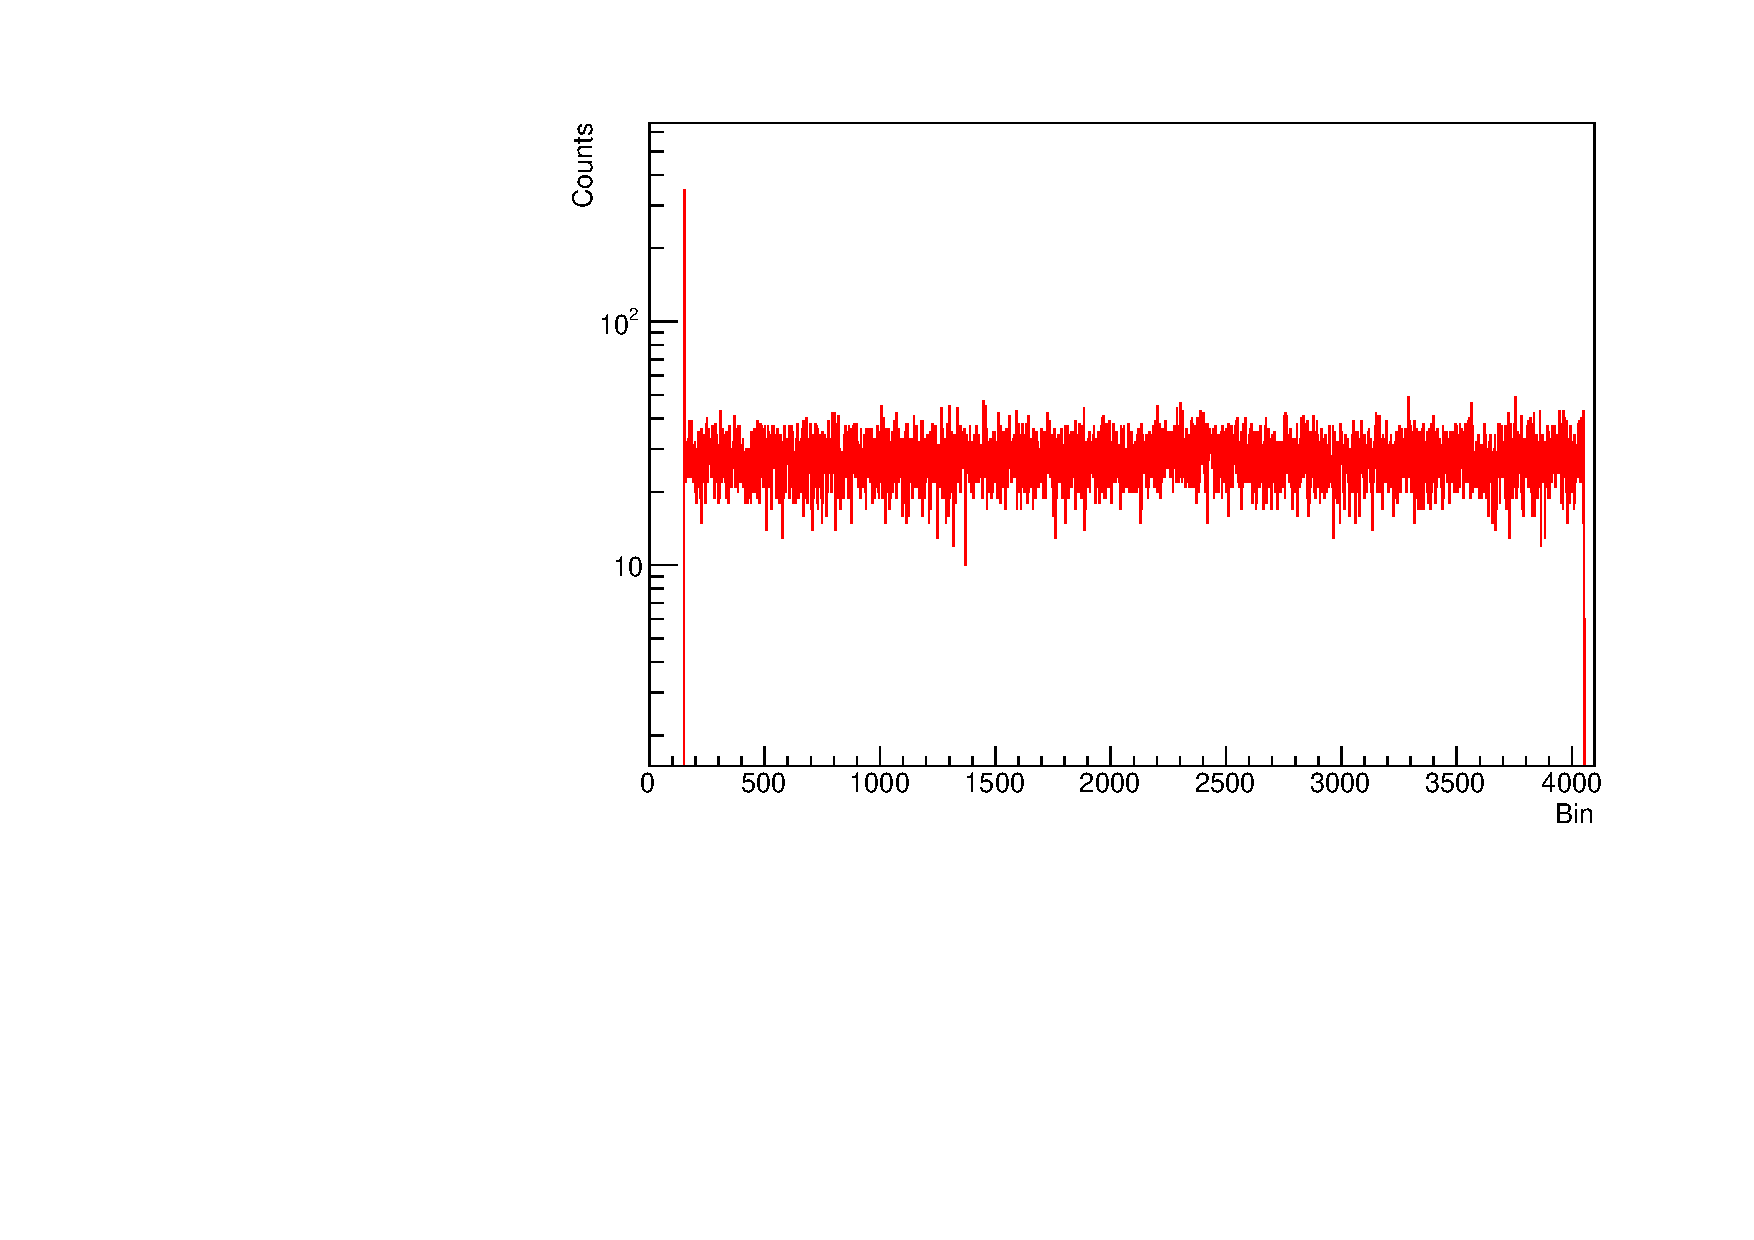
\includegraphics[scale=0.374]{img/bkg_sx.pdf}}
  \caption{Prima analisi dello spettro di ritardi temporali generati uniformemente; si nota la presenza di un eccesso di eventi indesiderato nell'intervallo $[2200,2700]$ (è stato applicato un rebin di un fattore 12 per evidenziare meglio la situazione).}
  \label{rumore1}
\end{figure}
%

Il TAC nr.~437 sembra presentare due problemi, un picco all'inizio dello spettro di cui non si è scoperta l'origine, ma che non influisce sulla raccolta dati e un eccesso di eventi nell'intervallo $[2200,2700]$. Questo secondo problema di origine anch'essa ignota rappresenta invece un potenziale fattore di disturbo per l'analisi dati, Un possibile approccio alla risoluzione verrà presentato in sezione ???.

Dopo questa prima fase si è verificato che il TAC  non erogasse più di 5 V (il massimo valore di tensione convertibile dall'ADC) in corrispondenza di un ritardo di 20 $\mu$s. Si è proceduto quindi a verificare la linearità della catena elettronica TAC + ADC e ottenere quindi una calibrazione temporale dello spettro registrato dal multicanale: tramite due copie del segnale di un impulsatore opportunamente discriminato fornite in input al TAC, separate da una distanza temporale variabile nel range $[0 \ \mu \mbox{s},20 \ \mu \mbox{s}]$, si sono registrati i relativi valori di tensione erogati e il canale corrispondente (si veda appendice B, figure \ref{time_tens} e \ref{chan_time}).

Con il fondoscala impostato come descritto in precedenza, il TAC eroga per valori del ritardo compresi tra 60 ns e 20 $\mu$s segnali nei range di tensione $[0.211 \ \mbox{V}, 5.070 \ \mbox{V}]$.
%
%
\section{Operazioni preliminari alla presa dati}
\subsection{Conteggi in coincidenza}
La fase di studio successiva consiste nel raccogliere i conteggi in coincidenza tra varie \emph{slab} e conseguentemente ottimizzare i valori di tensione applicata ai fotomoltiplicatori al fine di ottenere valori uniformi tra loro e in linea con le previsioni teoriche (vedi appendice A). 
Innanzitutto, si sono scelti i seguenti valori di tensione dei PMT: 
\begin{table}[h]
		\centering
	\begin{tabular}{ccc}
		\toprule
		PMT	&	HV [V]	&	Frequenza [Hz]\\	
		\midrule
		1	&	1860	&	109	\\
		2	&	1940	&	91	\\
		3	&	1930	&	100	\\
		4	&	1920	&	121	\\
		5	&	1890	&	121	\\
		6	&	1950	&	105	\\
		7	&	1770	&	123	\\
		8	&	1890	&	173	\\
		9	&	1670	&	128	\\
		10	&	1810	&	101	\\
		11	&	1750	&	124	\\
		12	&	1840	&	82	\\
		13	&	1960	&	86	\\
		14	&	1800	&	197	\\
		\bottomrule
	\end{tabular}
	\caption{Tensione finale applicata ai fotomoltiplicatori e relativo numero di conteggi con il piombo posizionato, L'incertezza associata a ciascuna frequenza è di 1 Hz. Le tensioni scelte garantiscono la condizione di \emph{plateau} da distante rispetto al fototubo.}
	\label{HV_counts}
\end{table}
Si sono quindi raccolti i dati di varie coincidenze, prima senza e poi sovrapponedo il piombo, per testare la diminuzione di eventi rivelati in presenza delle lastre, e verificare che la geometria dell'apparato fosse consistente con il numero di eventi raccolti. I simboli L e R indicano rispettivamente R $= 14 \vee 11 $ e L $= 12 \vee 13$, e insieme alla coppia di PMT 3 e PMT 4 (cioè, S5) formano la cosiddetta \emph{scatola}, utile per i circuiti di START e STOP, analizzati nel paragrafo successivo.
%
\begin{table}[H]
	\centering
	\begin{tabular}{ccc}
		\toprule
		Coincidenze						&	Frequenza senza Pb [Hz] & Frequenza con Pb [Hz]	\\
		\midrule
		S1 (PMT1 $\wedge$ PMT2)					& $60.6 \pm 0.8$	& $52.0 \pm 0.7$ \\
		S2 (PMT9 $\wedge$ PMT10)				& $64.1 \pm 0.8$	& $60.0 \pm 0.8$ \\
		S3 (PMT7 $\wedge$ PMT8)					& $77.2 \pm 0.9$	& $75.1 \pm 0.9$ \\
		S4 (PMT5 $\wedge$ PMT6)					& $63.4 \pm 0.8$	& $61.5 \pm 0.8$ \\
		S5 (PMT3 $\wedge$ PMT4)					& $61.1 \pm 0.8$	& $60.3 \pm 0.8$ \\
		S1 $\wedge$ S2 						& $39.0 \pm 0.6$	& $36.2 \pm 0.6$ \\
		S2 $\wedge$ S3 						& $37.9 \pm 0.6$    	& $36.4 \pm 0.6$ \\
		S3 $\wedge$ S4 						& $37.5 \pm 0.6$	& $36.3 \pm 0.6$ \\
		S4 $\wedge$ S5 						& $36.0 \pm 0.6$	& $35.3 \pm 0.6$ \\
		S1 $\wedge$ S3 						& $29.2 \pm 0.5$	& $26.9 \pm 0.5$ \\
		S1 $\wedge$ S4 						& $22.9 \pm 0.5$	& $21.0 \pm 0.5$ \\
		S1 $\wedge$ S5 						& $17.7 \pm 0.4$	& $16.0 \pm 0.4$ \\
		S1 $\wedge$ S2 $\wedge$ S3				& $29.1 \pm 0.5$	& $27.5 \pm 0.5$ \\
		S2 $\wedge$ S3 $\wedge$ S4				& $28.7 \pm 0.5$	& $27.8 \pm 0.5$ \\
		S3 $\wedge$ S4 $\wedge$ S5				& $28.6 \pm 0.5$	& $27.6 \pm 0.5$ \\
		S1 $\wedge$ S2 $\wedge$ S3 $\wedge$ S4			& $21.8 \pm 0.5$	& $21.8 \pm 0.5$ \\
		S2 $\wedge$ S3 $\wedge$ S4 $\wedge$ S5			& $20.8 \pm 0.5$	& $21.0 \pm 0.5$ \\
		S1 $\wedge$ S2 $\wedge$ S3 $\wedge$ S4 $\wedge$ S5	& $16.7 \pm 0.4$	& $16.7 \pm 0.4$ \\	
		S1 $\wedge$ S2 $\wedge$ L				& $8.9 \pm 0.3$		& $8.8 \pm 0.3$	\\
		S1 $\wedge$ S2 $\wedge$ R				& $8.4 \pm 0.3$		& $7.7 \pm 0.3$	\\
		S3 $\wedge$ S4 $\wedge$ L				& $7.5 \pm 0.3$		& $8.0 \pm 0.3$	\\
		S3 $\wedge$ S4 $\wedge$ R				& $9.2 \pm 0.3$ 	& $9.3 \pm 0.3$	\\
		S1 $\wedge \ (\overline{\mbox{S5}\vee \mbox{L} \vee \mbox{R}})$ (veto)	& $51.3 \pm 0.7$	& $43.2 \pm 0.7$	\\
		\bottomrule
	\end{tabular}
	\caption{Coincidenze. 
	Si noti che nell'ultima misura si è utilizzato il veto per negare il segnale, 
	in quanto esso è risultato più efficiente dell'uscita negata dei discriminatori 
	nell'individuare il segnale voluto: talvolta, infatti, l'uscita negata dei discriminatori non forniva in uscita il segnale desiderato, 
	probabilmente a causa di un malfunzionamento dei moduli o di un problema nella temporizzazione dei segnali. Per ovviare a ciò, con riferimento all'ultima coincidenza,
	si è messo il segnale $S5\vee L\vee R$ (opportunamente temporizzato)
	nell'ingresso di veto del discriminatore del 
	segnale $S1$: qualora il veto fosse stato attivo, l'output 
	sarebbe stato nullo.}
	\label{coincidenze}
\end{table}
%
\subsection{Costruzione del circuito}
A questo punto, dopo tutte le verifiche necessarie, e dopo aver ripetuto le prove di luce-buio\footnote{Si è notato un eccesso di segnale proveniente da una zona della \emph{slab} superiore, subito risolto con dello scotch isolante.}, si sono costruiti i circuiti di START e di STOP, per la rivelazione dei muoni cosmici. Si rende però necessario fare una premessa: potendo utilizzare nella costruzione del circuito segnali negati o di veto, dopo alcune prove si è optato per la seconda possibilità, avendo cura di temporizzare bene le coincidenze, ossia facendo in modo che il segnale di veto rendesse effettivamente cieco l'apparato. In questo passaggio il segnale di veto è stato ritardato e allargato cosicchè contenesse il segnale del PMT in coincidenza.

Per il segnale di START, corrispondente al muone che entra dall'alto e non esce dalla \emph{scatola}, si è partiti considerando varie possibilità; il miglior compromesso, che generasse un segnale sufficientemente pulito ma con una frequenza di conteggio non troppo bassa, si è rivelato essere il segnale S1 $\wedge$ S2  $\wedge$ $\overline{\mbox{S5}\vee \mbox{L} \vee \mbox{R}}$ , la cui frequenza in coincidenza è 6.6 Hz.
Il segnale di STOP corrisponde invece all'avvenuto decadimento e rivelazione dell'elettrone emesso, ed è stato scelto essere (S3 $\veebar$ S4)  $\wedge$ $\overline{\mbox{S1} \vee \mbox{S5}\vee \mbox{L} \vee \mbox{R}}$, con frequenza 38.1 Hz (schemi in figura \ref{scemi}).

A questo punto, con i segnali START e STOP fisici si sono ripetute i test di uniformità descritti alla sezione \ref{tac} utilizzando START artificiale con STOP fisico e viceversa. Si riscontra lo stesso eccesso di eventi attorno al canale 2500 individuato durante la caratterizzazione del TAC.
%
\begin{figure}[h]
	\centering
	 \subfloat[START.]
 {\begin{circuitikz}
      \draw 
      (0.5,10.97)  to[short,o-] (1.5,10.97)
      (0.5,11.53)  to[short, o-] (1.5,11.53)
      (2.88,11.25) node[american and port] {}
		   node[left=6pt] {\tiny{AND}}
      (0.5,10.97) node[below] {S2}
      (0.5,11.53) node[above] {S1}
      (3.03,11.25) to [short,-o] (5.3, 11.25)
      (2.5,6.97)  to[short,o-] (3.5,6.97)
      (2.3,7.25)  to[short,o-] (3.93,7.25)
      (2.5,7.53)  to[short, o-] (3.5,7.53)
      (2.5,6.97) node[below] {L}
      (2.5,7.53) node[above] {R}
      (2,7.25) node[] {S5}     
      (4.88,7.25) node[american or port] {}
                  node[left=6pt] {\tiny{OR}}
      (5.03,7.25) to[short] (5.03, 11.25)
      (4.85, 10.60) node[rotate=90] {\scriptsize{VETO}}
      ;
    \end{circuitikz}}
    \hspace{1.5 cm}
\subfloat[STOP.]
{\begin{circuitikz}
      \draw 
      (0.5,10.97)  to[short,o-] (1.5,10.97)
      (0.5,11.53)  to[short, o-] (1.5,11.53)
      (2.88,11.25) node[american or port] {}
		   node[left=6pt] {\tiny{OR}}
      (3.4,9.15) node[american and port] {}
		 node[left=6pt] {\tiny{AND}}
      (1, 8.87) to[short] (1, 10.97)
      (1, 8.87) to[short] (2.03, 8.87)
      (1.3, 9.43) to[short] (1.3, 11.53)
      (1.3, 9.43) to[short] (2.03, 9.43)
      (3.55, 9.15) to[short] (4.2, 9.15)
      (4.2, 9.15) to[short] (4.2,7.73)
      (0.5,10.97) node[below] {S4}
      (0.5,11.53) node[above] {S3}
      (3.03,11.25) to [short,-o] (5.3, 11.25)
      (2.5,6.97)  to[short,o-] (3.5,6.97)
      (2.3,7.15)  to[short,o-] (3.93,7.15)
      (2.3,7.35)  to[short,o-] (3.93,7.35)
      (2.5,7.53)  to[short, o-] (3.5,7.53)
      (2.5,6.97) node[below] {L}
      (2.5,7.53) node[above] {R}
      (1.9,7.07) node[] {S1}     
      (1.9,7.43) node[] {S5}   
      (4.88,7.25) node[american or port] {}
		  node[left=6pt] {\tiny{OR}}
      (5.03,7.25) to[short] (5.03, 11.25)
      (4.85, 10.60) node[rotate=90] {\scriptsize{VETO}}
           ;
    \end{circuitikz}}

	\caption{Schema dei circuiti di START e di STOP. Si noti che nel circuito di STOP si è utilizzato un segnale di XOR, ossia il veto ha una componente che rende cieco l'apparato quando entrambe le \emph{slab} S3 e S4 rivelano un evento; ciò viene utilizzato per cercare di incrementare la probabilità che il segnale di STOP non sia dato da un evento spurio, assumendo che una volta decaduto il muone l'elettrone si fermi alla prima \emph{slab} che incontra.}
	\label{scemi}
\end{figure}
%
\section{Analisi dati preliminare}
Dopo aver impostato il circuito come illustrato precedentemente, si è proceduto all'acquisizione dei dati relativi al ritardo che intercorre tra il passaggio del muone cosmico attraverso l'apparato di START e l'uscita dell'elettrone di decadimento attraverso lo STOP.

I dati consistono di tre acquisizioni, per un totale di circa 75000 eventi, riguardanti due popolazioni differenti di muoni\footnote{Dati presi da K.A. Olive \emph{et al.} (Particle Data Group), Chin. Phys. C, \textbf{38}, 090001 (2014) and 2015 update.}:
\begin{itemize}
	\item i $\mu^+$, tali che $\mbox{Br}(\mu^+ \to e^+\nu_e\overline{\nu}_\mu)\simeq 100 \%$ e aventi una vita media \linebreak $\tau^+=(2.1969811 \pm 0.0000022)\;\mu\mbox{s}$;
\item i $\mu^-$, i quali però si comportano in maniera differente. Essi, infatti, oltre a decadere nel canale $\mu^-\to e^-\overline{\nu}_e\nu_\mu$, possono sostituirsi ad un elettrone degli atomi del mezzo, formando un atomo muonico in uno stato metastabile che favorisce il processo di cattura $\mu^-+p\to n+\nu_\mu $, con $p$ protone del nucleo del mezzo. Questa implica una diminuzione della vita media per i $\mu^-$ al valore $\tau^-=(0.88 \pm 0.01) \ \mu \mbox{s}$.
\end{itemize}

I vari contributi possono essere convogliati nella seguente formula, che modellizza lo spettro che si ottiene tramite l'ADC:
 \[  \frac{dN}{dt} = A^+ e^{-t/\tau^+} + A^- e^{-t/\tau^-} + \mbox{\emph{bkg\;.}} \]
Queste due popolazioni vanno ovviamente considerate in maniera separata, sapendo che lo spettro raccolto prevede una prima parte relativa ai $\mu^-$ (per $t<4\tau^-$), una seconda parte relativa ai soli $\mu^+$ (per $4\tau^-<t<4\tau^+$) ed infine puro fondo (per $t>4\tau^+$), distinguibili grazie alla calibrazione temporale del sistema TAC+ADC.
L'analisi dati si svolge in base ai seguenti step:
%%%%%%%%%%%%%%%%%%%%%%%%%%%%%%
\begin{enumerate}
	\item si definisce un istogramma con 4096 canali, nel quale inserire tutta la statistica raccolta, assegnando a ciascun bin un contenuto pari alla somma dei contenuti del medesimo canale delle varie acquisizioni (in questo caso 3);
	\item si stima il fondo come la media tra i contenuti dei bin a partire da quello che, in base alla calibrazione, coincide con $t=4\tau^+$, e tale valore si sottrae al contenuto di ciascun bin;
	\item si definisce la funzione $f(t)=Ae^{-t/\tau}$, dove la variabile indipendente $t$ e $\tau$ si riferiscono a grandezze in canali; quindi si esegue un fit dell'istogramma nella regione dei soli $\mu^+$. Questa operazione permette di ricavare sia la vita media $\tau^+$ che l'abbondanza $A^+$ dei $\mu^+$; 
	\item al contenuto di ciascun canale dell'istogramma si sottrae il valore assunto dalla funzione suddetta in corrispondenza del centroide di ciascun canale, in modo tale da ricavare la distribuzione dei soli $\mu^-$;
	\item si effettua il fit dell'istogramma risultante, ricavando i parametri relativi ai $\mu^-$.
\end{enumerate}
%%%%%%%%%%%%%%%%%%%%%%%%%%%%%%
Questo procedimento presenta tuttavia un aspetto critico, da mettere a punto nella seconda parte dell'esperienza. 
Il fit della regione relativa ai $\mu^+$ riguarda canali dell'istogramma con bassa statistica e questo provoca una notevole fluttuazione dei risultati, in particolare al variare del numero di bin. 

Per quanto riguarda il rapporto numerico $N^+/N^-$ tra le due popolazioni, la stima è stata ottenuta tramite la seguente formula: 
\[\frac{A^+}{A^-}= \bigg ( \frac{\tau^+}{\tau^-} \bigg )  ^{-1} \frac{N^+}{N^-} \bigg ( \frac{\Gamma_d}{\Gamma_d+\Gamma_c} \bigg )^{-1}e^{t^*\left(\frac{1}{\tau^+}-\frac{1}{\tau^-}\right)}\sim\frac{N^+}{N^-}\]
dove $\Gamma_d$ e $\Gamma_c$ sono rispettivamente le larghezze parziali di decadimento e cattura per entrambe le popolazioni, mentre il termine esponenziale è stato aggiunto per tenere conto del fatto che l'apparato è cieco per un tempo $t^* \sim 150$ ns precedente allo zero.
%
\begin{figure}[h!]
\centering
\subfloat[][{Eventi raccolti.}]
{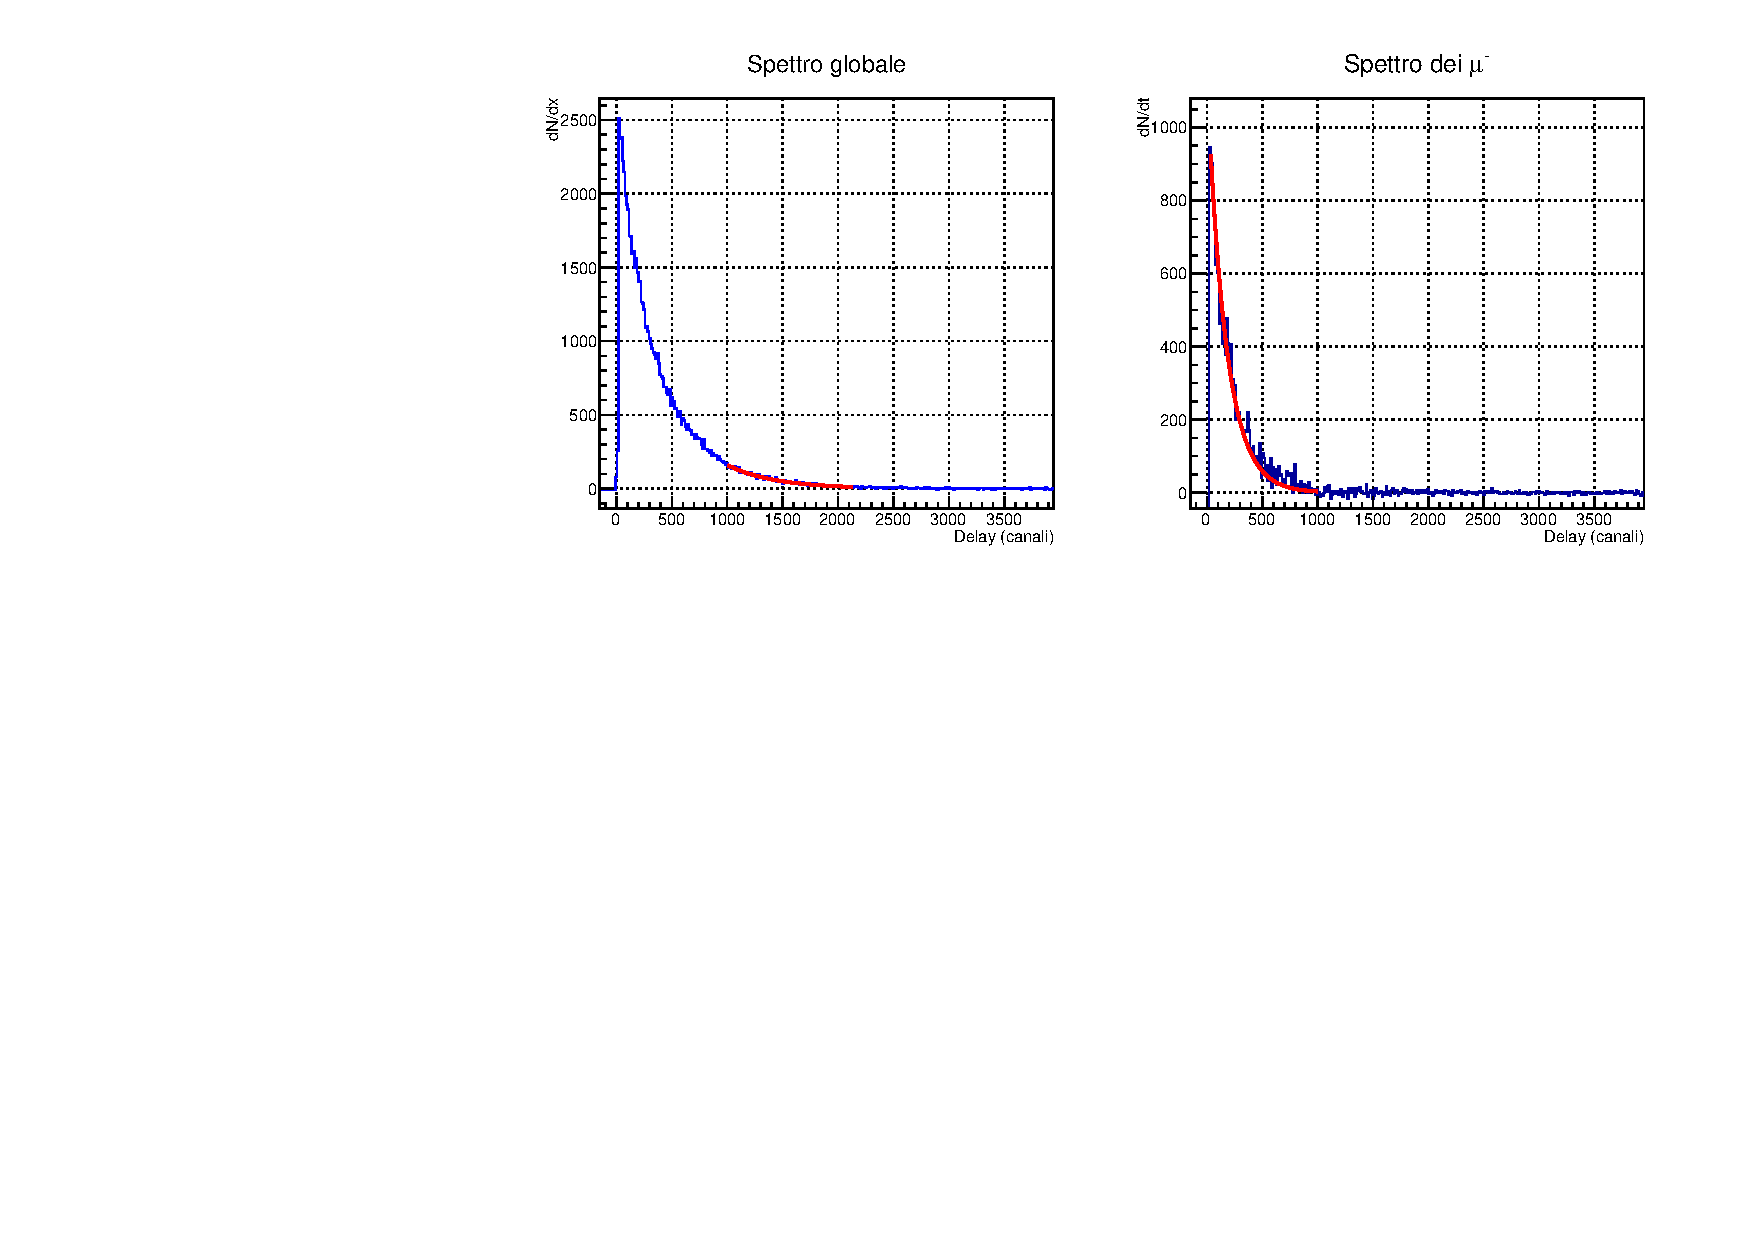
\includegraphics[width=1\textwidth]{img/Spettro_rebin12.pdf}} \\
\subfloat[][{Istogrammi sovrapposti}.]
{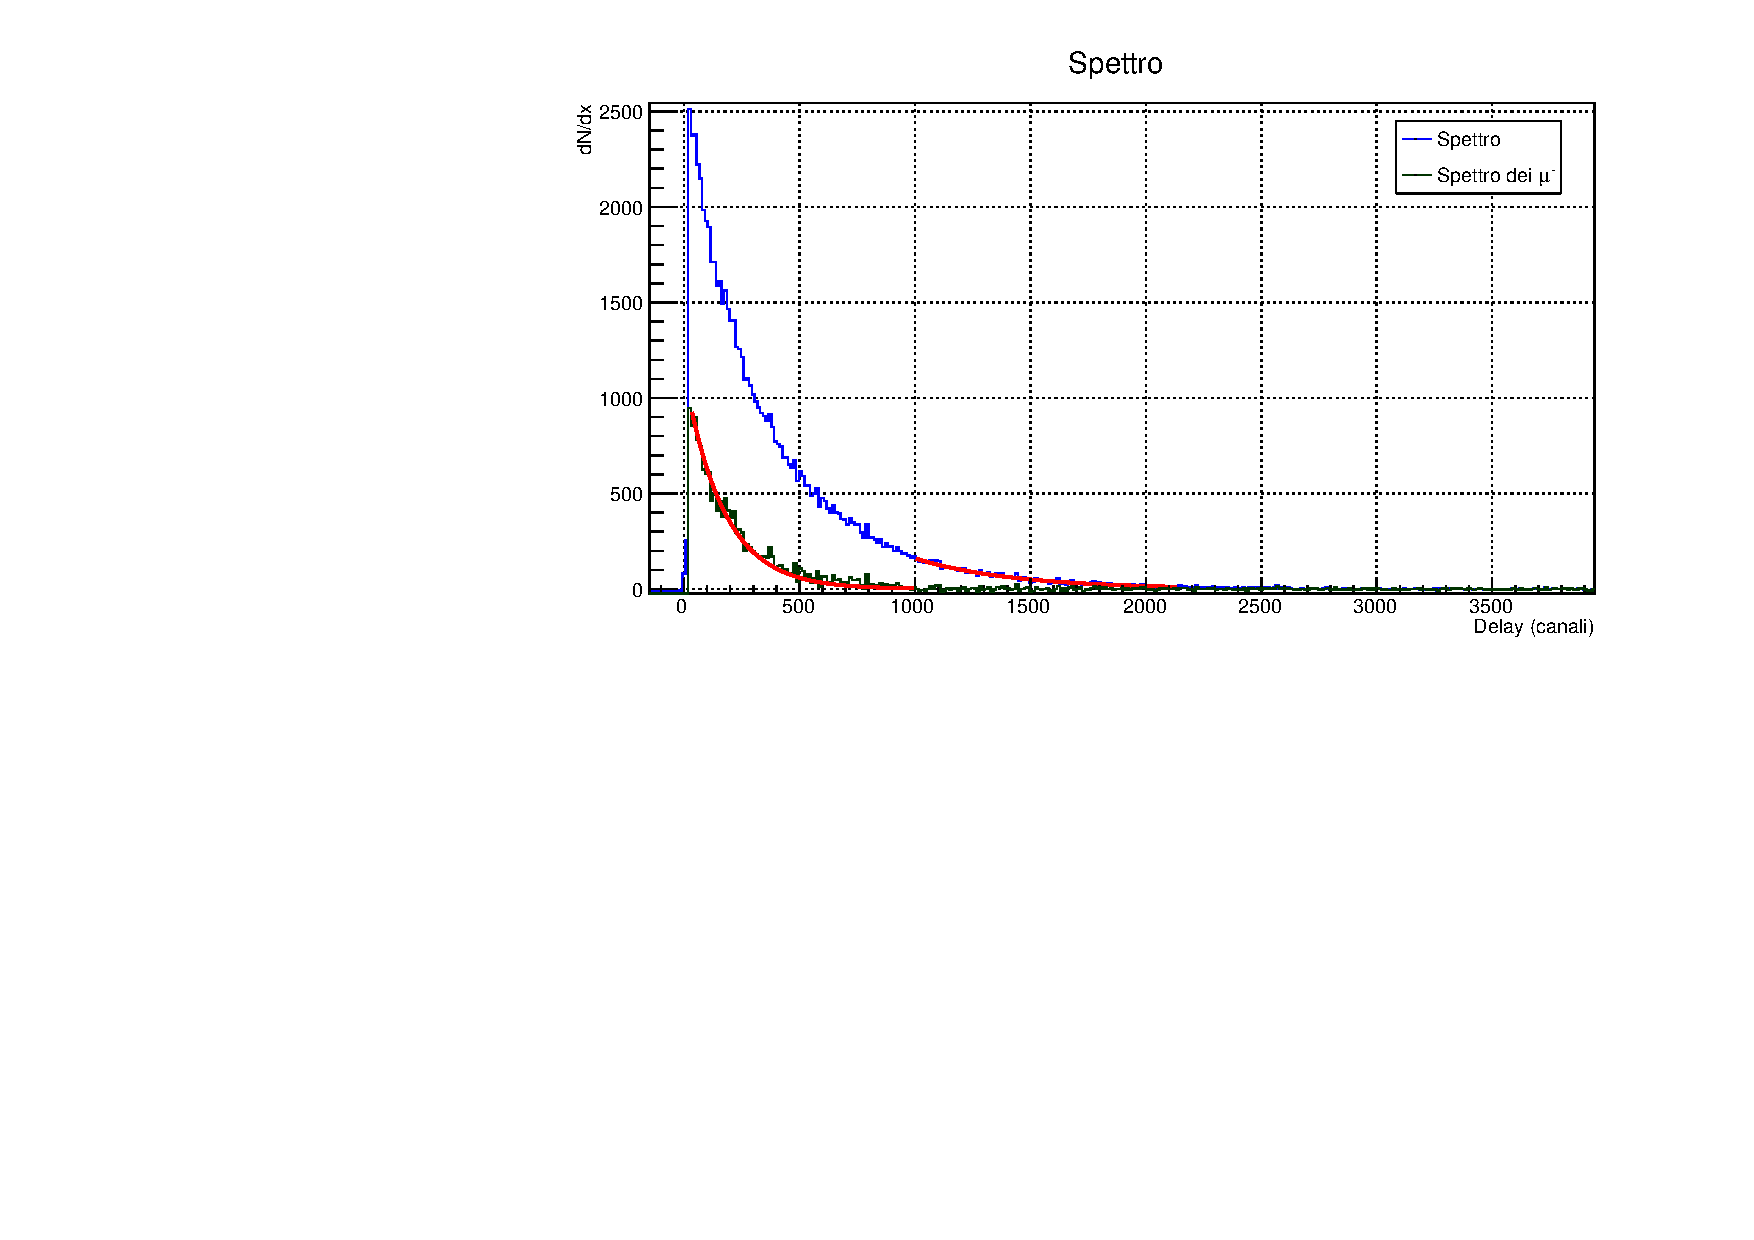
\includegraphics[width=1\textwidth]{img/histo_sovrapposti.pdf}} \\
\caption{Istogrammi dei dati raccolti e analizzati secondo quanto spiegato precedentemente, con un coefficiente di rebin 12.}
\label{fig::histo}
\end{figure}
%
In figura \ref{fig::histo} viene riportato il grafico degli eventi raccolti, dove l'istogramma ha un numero di bin ridotto di un fattore 12 rispetto a quello originale, appunto per ridurre le fluttuazioni statistiche in maniera ottimale. I risultati derivanti da questa analisi sono riportati in tabella \ref{results}.
\begin{table}[h!]
	\centering
	\begin{tabular}{ccccc}
		\toprule
		& Misura [$\mu$s]	&	Valore atteso [$\mu$s]	 & Compatibilità & Differenza 	\\	
		\midrule
		$\tau^+$	&	$2.20\pm 0.05$ & $2.1969811 \pm 0.0000022$ & 0.16 & 0.0072134 $\mu$s	\\
		$\tau^-$	&	$0.870\pm 0.007$ & $0.88 \pm 0.01$ & 0.80 & 0.01 $\mu$s	\\
		$N^+/N^-$	&	$1.5 \pm 0.1$ & $1.261 \pm 0.009$ & 1.95 & 0.20	\\
		\bottomrule
	\end{tabular}
	\caption{Risultati dei fit (rebin 12).}
	\label{results}
\end{table}
%%%%%%%%%%%%%%%%%%%%%%%%%%%%%%%%%%%%%%%%%%%%%%%%%%%%%%%%%%%%%%%%%%%%%%%%%%%%%%%%%%%%%%%%%%%%%%%%%%%%%%%%%%%%%%%%%%%%%%%%%%%%%%%%%%%%%%%%%%%%%%%%%%%%%%%%%%%%%%%%%%%%%%%
\cleardoublepage
\section{Simulazione MonteCarlo e analisi dati}
Lo scopo di questa fase dell'esperimento consiste nella ricerca e messa a punto di un metodo sperimentale di analisi degli spettri raccolti. Il lavoro si suddivide in due step:
\begin{enumerate}
 \item sviluppare un codice di simulazione MonteCarlo (MC) in ambiente ROOT nel quale si simulano molti spettri di decadimento dei muoni cosmici in un range utile di circa 3900 canali, in accordo con gli spettri acquisiti. Gli istogrammi simulati vengono quindi utilizzati per testare diversi metodi di fit per l'estrazione dei parametri fisici;
 \item utilizzare il metodo di fit stabilito nello step precedente per estrarre $\tau^+$, $\tau^-$ e $R=N^+/N^-$ dagli spettri raccolti.
\end{enumerate}
%
\subsection{Simulazione del fondo}
La prima versione del metodo MC prevede la simulazione di spettri costituiti da solo rumore di fondo (avente una distribuzione uniforme su tutto lo spettro che da ora in avanti chameremo anche \textit{baseline}), attraverso la generazione uniforme di numeri casuali (\lstinline{TRandom3::Uniform(double Begin,double End)}). 
I metodi testati per la stima della \textit{baseline} sono i seguenti:
\begin{enumerate}
 \item media aritmetica dei contenuti dei bin dell'istogramma \lstinline{baseline};
 \item fit con il metodo del $\chi^2$ utilizzando la funzione \lstinline{pol0} (\lstinline{baseline.Fit("pol0")});
 \item metodo della maximum likelihood utilizzando la funzione \newline \lstinline{pol0} (\lstinline{baseline.Fit("pol0","L")}).
\end{enumerate}
%
\begin{figure}[H]
 \centerline{%
 \begin{adjustbox}{width=\linewidth+1cm}
 \documentclass{standalone}
\usepackage{tikz}
\begin{document}
\begin{tikzpicture}
\pgfdeclareplotmark{cross} {
\pgfpathmoveto{\pgfpoint{-0.3\pgfplotmarksize}{\pgfplotmarksize}}
\pgfpathlineto{\pgfpoint{+0.3\pgfplotmarksize}{\pgfplotmarksize}}
\pgfpathlineto{\pgfpoint{+0.3\pgfplotmarksize}{0.3\pgfplotmarksize}}
\pgfpathlineto{\pgfpoint{+1\pgfplotmarksize}{0.3\pgfplotmarksize}}
\pgfpathlineto{\pgfpoint{+1\pgfplotmarksize}{-0.3\pgfplotmarksize}}
\pgfpathlineto{\pgfpoint{+0.3\pgfplotmarksize}{-0.3\pgfplotmarksize}}
\pgfpathlineto{\pgfpoint{+0.3\pgfplotmarksize}{-1.\pgfplotmarksize}}
\pgfpathlineto{\pgfpoint{-0.3\pgfplotmarksize}{-1.\pgfplotmarksize}}
\pgfpathlineto{\pgfpoint{-0.3\pgfplotmarksize}{-0.3\pgfplotmarksize}}
\pgfpathlineto{\pgfpoint{-1.\pgfplotmarksize}{-0.3\pgfplotmarksize}}
\pgfpathlineto{\pgfpoint{-1.\pgfplotmarksize}{0.3\pgfplotmarksize}}
\pgfpathlineto{\pgfpoint{-0.3\pgfplotmarksize}{0.3\pgfplotmarksize}}
\pgfpathclose
\pgfusepathqstroke
}
\pgfdeclareplotmark{cross*} {
\pgfpathmoveto{\pgfpoint{-0.3\pgfplotmarksize}{\pgfplotmarksize}}
\pgfpathlineto{\pgfpoint{+0.3\pgfplotmarksize}{\pgfplotmarksize}}
\pgfpathlineto{\pgfpoint{+0.3\pgfplotmarksize}{0.3\pgfplotmarksize}}
\pgfpathlineto{\pgfpoint{+1\pgfplotmarksize}{0.3\pgfplotmarksize}}
\pgfpathlineto{\pgfpoint{+1\pgfplotmarksize}{-0.3\pgfplotmarksize}}
\pgfpathlineto{\pgfpoint{+0.3\pgfplotmarksize}{-0.3\pgfplotmarksize}}
\pgfpathlineto{\pgfpoint{+0.3\pgfplotmarksize}{-1.\pgfplotmarksize}}
\pgfpathlineto{\pgfpoint{-0.3\pgfplotmarksize}{-1.\pgfplotmarksize}}
\pgfpathlineto{\pgfpoint{-0.3\pgfplotmarksize}{-0.3\pgfplotmarksize}}
\pgfpathlineto{\pgfpoint{-1.\pgfplotmarksize}{-0.3\pgfplotmarksize}}
\pgfpathlineto{\pgfpoint{-1.\pgfplotmarksize}{0.3\pgfplotmarksize}}
\pgfpathlineto{\pgfpoint{-0.3\pgfplotmarksize}{0.3\pgfplotmarksize}}
\pgfpathclose
\pgfusepathqfillstroke
}
\pgfdeclareplotmark{newstar} {
\pgfpathmoveto{\pgfqpoint{0pt}{\pgfplotmarksize}}
\pgfpathlineto{\pgfqpointpolar{44}{0.5\pgfplotmarksize}}
\pgfpathlineto{\pgfqpointpolar{18}{\pgfplotmarksize}}
\pgfpathlineto{\pgfqpointpolar{-20}{0.5\pgfplotmarksize}}
\pgfpathlineto{\pgfqpointpolar{-54}{\pgfplotmarksize}}
\pgfpathlineto{\pgfqpointpolar{-90}{0.5\pgfplotmarksize}}
\pgfpathlineto{\pgfqpointpolar{234}{\pgfplotmarksize}}
\pgfpathlineto{\pgfqpointpolar{198}{0.5\pgfplotmarksize}}
\pgfpathlineto{\pgfqpointpolar{162}{\pgfplotmarksize}}
\pgfpathlineto{\pgfqpointpolar{134}{0.5\pgfplotmarksize}}
\pgfpathclose
\pgfusepathqstroke
}
\pgfdeclareplotmark{newstar*} {
\pgfpathmoveto{\pgfqpoint{0pt}{\pgfplotmarksize}}
\pgfpathlineto{\pgfqpointpolar{44}{0.5\pgfplotmarksize}}
\pgfpathlineto{\pgfqpointpolar{18}{\pgfplotmarksize}}
\pgfpathlineto{\pgfqpointpolar{-20}{0.5\pgfplotmarksize}}
\pgfpathlineto{\pgfqpointpolar{-54}{\pgfplotmarksize}}
\pgfpathlineto{\pgfqpointpolar{-90}{0.5\pgfplotmarksize}}
\pgfpathlineto{\pgfqpointpolar{234}{\pgfplotmarksize}}
\pgfpathlineto{\pgfqpointpolar{198}{0.5\pgfplotmarksize}}
\pgfpathlineto{\pgfqpointpolar{162}{\pgfplotmarksize}}
\pgfpathlineto{\pgfqpointpolar{134}{0.5\pgfplotmarksize}}
\pgfpathclose
\pgfusepathqfillstroke
}
\definecolor{c}{rgb}{1,1,1};
\draw [color=c, fill=c] (0,0) rectangle (20,10.9474);
\draw [color=c, fill=c] (0.187135,5.59115) rectangle (6.45614,10.8379);
\draw [color=c, fill=c] (0.814035,6.11582) rectangle (5.82924,10.3132);
\definecolor{c}{rgb}{0,0,0};
\draw [c,line width=0.9] (0.814035,6.11582) -- (0.814035,10.3132) -- (5.82924,10.3132) -- (5.82924,6.11582) -- (0.814035,6.11582);
\definecolor{c}{rgb}{1,1,1};
\draw [color=c, fill=c] (0.814035,6.11582) rectangle (5.82924,10.3132);
\definecolor{c}{rgb}{0,0,0};
\draw [c,line width=0.9] (0.814035,6.11582) -- (0.814035,10.3132) -- (5.82924,10.3132) -- (5.82924,6.11582) -- (0.814035,6.11582);
\definecolor{c}{rgb}{0,0,0.6};
\draw [c,line width=0.9] (0.814035,6.15058) -- (0.914339,6.15058) -- (0.914339,6.11582) -- (1.01464,6.11582) -- (1.01464,6.15058) -- (1.11495,6.15058) -- (1.11495,6.28963) -- (1.21525,6.28963) -- (1.21525,6.39391) -- (1.31556,6.39391) --
 (1.31556,6.42867) -- (1.41586,6.42867) -- (1.41586,6.46343) -- (1.51616,6.46343) -- (1.51616,6.39391) -- (1.61647,6.39391) -- (1.61647,6.63724) -- (1.71677,6.63724) -- (1.71677,6.53295) -- (1.81708,6.53295) -- (1.81708,6.74152) -- (1.91738,6.74152)
 -- (1.91738,6.98485) -- (2.01768,6.98485) -- (2.01768,7.40198) -- (2.11799,7.40198) -- (2.11799,7.05437) -- (2.21829,7.05437) -- (2.21829,7.85387) -- (2.3186,7.85387) -- (2.3186,7.9234) -- (2.4189,7.9234) -- (2.4189,8.27101) -- (2.5192,8.27101) --
 (2.5192,8.65338) -- (2.61951,8.65338) -- (2.61951,9.31384) -- (2.71981,9.31384) -- (2.71981,9.14003) -- (2.82012,9.14003) -- (2.82012,9.90478) -- (2.92042,9.90478) -- (2.92042,9.62669) -- (3.02073,9.62669) -- (3.02073,9.3486) -- (3.12103,9.3486) --
 (3.12103,9.3486) -- (3.22133,9.3486) -- (3.22133,10.1133) -- (3.32164,10.1133) -- (3.32164,9.41812) -- (3.42194,9.41812) -- (3.42194,9.73097) -- (3.52225,9.73097) -- (3.52225,9.76573) -- (3.62255,9.76573) -- (3.62255,9.41812) -- (3.72285,9.41812) --
 (3.72285,8.34053) -- (3.82316,8.34053) -- (3.82316,8.79242) -- (3.92346,8.79242) -- (3.92346,7.99292) -- (4.02377,7.99292) -- (4.02377,8.79242) -- (4.12407,8.79242) -- (4.12407,8.13196) -- (4.22437,8.13196) -- (4.22437,7.2977) -- (4.32468,7.2977) --
 (4.32468,7.22817) -- (4.42498,7.22817) -- (4.42498,6.8458) -- (4.52529,6.8458) -- (4.52529,6.81104) -- (4.62559,6.81104) -- (4.62559,6.98485) -- (4.72589,6.98485) -- (4.72589,6.46343) -- (4.8262,6.46343) -- (4.8262,6.46343) -- (4.9265,6.46343) --
 (4.9265,6.35915) -- (5.02681,6.35915) -- (5.02681,6.15058) -- (5.12711,6.15058) -- (5.12711,6.25486) -- (5.22742,6.25486) -- (5.22742,6.15058) -- (5.32772,6.15058) -- (5.32772,6.15058) -- (5.42802,6.15058) -- (5.42802,6.11582) -- (5.52833,6.11582)
 -- (5.52833,6.11582) -- (5.62863,6.11582) -- (5.62863,6.11582) -- (5.72894,6.11582) -- (5.72894,6.15058) -- (5.82924,6.15058);
\definecolor{c}{rgb}{1,0,0};
\draw [c,line width=1.8] (0.88876,6.13912) -- (0.937908,6.14464) -- (0.987056,6.1513) -- (1.0362,6.1593) -- (1.08535,6.16887) -- (1.1345,6.18024) -- (1.18365,6.1937) -- (1.2328,6.20954) -- (1.28194,6.22809) -- (1.33109,6.2497) -- (1.38024,6.27476) --
 (1.42939,6.30364) -- (1.47854,6.33676) -- (1.52768,6.37455) -- (1.57683,6.41743) -- (1.62598,6.46581) -- (1.67513,6.52012) -- (1.72428,6.58073) -- (1.77342,6.648) -- (1.82257,6.72225) -- (1.87172,6.80371) -- (1.92087,6.89258) -- (1.97002,6.98896) --
 (2.01917,7.09283) -- (2.06831,7.20411) -- (2.11746,7.32255) -- (2.16661,7.44782) -- (2.21576,7.57943) -- (2.26491,7.71673) -- (2.31405,7.85898) -- (2.3632,8.00525) -- (2.41235,8.15451) -- (2.4615,8.30557) -- (2.51065,8.45716) -- (2.55979,8.60788) --
 (2.60894,8.75628) -- (2.65809,8.90081) -- (2.70724,9.03993) -- (2.75639,9.17207) -- (2.80553,9.29569) -- (2.85468,9.4093) -- (2.90383,9.51149) -- (2.95298,9.60097) -- (3.00213,9.67658) -- (3.05127,9.73732) -- (3.10042,9.78238) -- (3.14957,9.81117)
 -- (3.19872,9.82328) -- (3.24787,9.81856) -- (3.29701,9.79707);
\draw [c,line width=1.8] (3.29701,9.79707) -- (3.34616,9.75909) -- (3.39531,9.70515) -- (3.44446,9.63597) -- (3.49361,9.55245) -- (3.54275,9.45569) -- (3.5919,9.34693) -- (3.64105,9.22754) -- (3.6902,9.09895) -- (3.73935,8.96271) -- (3.78849,8.82036)
 -- (3.83764,8.67347) -- (3.88679,8.52359) -- (3.93594,8.3722) -- (3.98509,8.22074) -- (4.03423,8.07054) -- (4.08338,7.92282) -- (4.13253,7.77869) -- (4.18168,7.63911) -- (4.23083,7.50491) -- (4.27997,7.37679) -- (4.32912,7.25529) --
 (4.37827,7.14083) -- (4.42742,7.03368) -- (4.47657,6.93401) -- (4.52572,6.84185) -- (4.57486,6.75714) -- (4.62401,6.67975) -- (4.67316,6.60945) -- (4.72231,6.54595) -- (4.77146,6.48892) -- (4.8206,6.43799) -- (4.86975,6.39274) -- (4.9189,6.35277) --
 (4.96805,6.31765) -- (5.0172,6.28695) -- (5.06634,6.26027) -- (5.11549,6.23719) -- (5.16464,6.21734) -- (5.21379,6.20035) -- (5.26294,6.18588) -- (5.31208,6.17363) -- (5.36123,6.1633) -- (5.41038,6.15464) -- (5.45953,6.14742) -- (5.50868,6.14142) --
 (5.55782,6.13647) -- (5.60697,6.1324) -- (5.65612,6.12907) -- (5.70527,6.12636);
\draw [c,line width=1.8] (5.70527,6.12636) -- (5.75442,6.12417);
\definecolor{c}{rgb}{0,0,0};
\draw [c,line width=0.9] (0.814035,6.11582) -- (5.82924,6.11582);
\draw [anchor= east] (5.82924,5.822) node[scale=0.832348, color=c, rotate=0]{B};
\draw [c,line width=0.9] (1.81071,6.24174) -- (1.81071,6.11582);
\draw [c,line width=0.9] (2.09143,6.17878) -- (2.09143,6.11582);
\draw [c,line width=0.9] (2.37215,6.17878) -- (2.37215,6.11582);
\draw [c,line width=0.9] (2.65287,6.17878) -- (2.65287,6.11582);
\draw [c,line width=0.9] (2.9336,6.17878) -- (2.9336,6.11582);
\draw [c,line width=0.9] (3.21432,6.24174) -- (3.21432,6.11582);
\draw [c,line width=0.9] (3.49504,6.17878) -- (3.49504,6.11582);
\draw [c,line width=0.9] (3.77576,6.17878) -- (3.77576,6.11582);
\draw [c,line width=0.9] (4.05648,6.17878) -- (4.05648,6.11582);
\draw [c,line width=0.9] (4.3372,6.17878) -- (4.3372,6.11582);
\draw [c,line width=0.9] (4.61793,6.24174) -- (4.61793,6.11582);
\draw [c,line width=0.9] (1.81071,6.24174) -- (1.81071,6.11582);
\draw [c,line width=0.9] (1.52999,6.17878) -- (1.52999,6.11582);
\draw [c,line width=0.9] (1.24927,6.17878) -- (1.24927,6.11582);
\draw [c,line width=0.9] (0.968544,6.17878) -- (0.968544,6.11582);
\draw [c,line width=0.9] (4.61793,6.24174) -- (4.61793,6.11582);
\draw [c,line width=0.9] (4.89865,6.17878) -- (4.89865,6.11582);
\draw [c,line width=0.9] (5.17937,6.17878) -- (5.17937,6.11582);
\draw [c,line width=0.9] (5.46009,6.17878) -- (5.46009,6.11582);
\draw [c,line width=0.9] (5.74081,6.17878) -- (5.74081,6.11582);
\draw [anchor=base] (1.81071,5.79577) node[scale=0.832348, color=c, rotate=0]{9.9};
\draw [anchor=base] (3.21432,5.79577) node[scale=0.832348, color=c, rotate=0]{10};
\draw [anchor=base] (4.61793,5.79577) node[scale=0.832348, color=c, rotate=0]{10.1};
\draw [c,line width=0.9] (0.814035,6.11582) -- (0.814035,10.3132);
\draw [c,line width=0.9] (0.964491,6.11582) -- (0.814035,6.11582);
\draw [c,line width=0.9] (0.889263,6.28963) -- (0.814035,6.28963);
\draw [c,line width=0.9] (0.889263,6.46343) -- (0.814035,6.46343);
\draw [c,line width=0.9] (0.889263,6.63724) -- (0.814035,6.63724);
\draw [c,line width=0.9] (0.964491,6.81104) -- (0.814035,6.81104);
\draw [c,line width=0.9] (0.889263,6.98485) -- (0.814035,6.98485);
\draw [c,line width=0.9] (0.889263,7.15865) -- (0.814035,7.15865);
\draw [c,line width=0.9] (0.889263,7.33246) -- (0.814035,7.33246);
\draw [c,line width=0.9] (0.964491,7.50626) -- (0.814035,7.50626);
\draw [c,line width=0.9] (0.889263,7.68007) -- (0.814035,7.68007);
\draw [c,line width=0.9] (0.889263,7.85387) -- (0.814035,7.85387);
\draw [c,line width=0.9] (0.889263,8.02768) -- (0.814035,8.02768);
\draw [c,line width=0.9] (0.964491,8.20148) -- (0.814035,8.20148);
\draw [c,line width=0.9] (0.889263,8.37529) -- (0.814035,8.37529);
\draw [c,line width=0.9] (0.889263,8.5491) -- (0.814035,8.5491);
\draw [c,line width=0.9] (0.889263,8.7229) -- (0.814035,8.7229);
\draw [c,line width=0.9] (0.964491,8.89671) -- (0.814035,8.89671);
\draw [c,line width=0.9] (0.889263,9.07051) -- (0.814035,9.07051);
\draw [c,line width=0.9] (0.889263,9.24432) -- (0.814035,9.24432);
\draw [c,line width=0.9] (0.889263,9.41812) -- (0.814035,9.41812);
\draw [c,line width=0.9] (0.964491,9.59193) -- (0.814035,9.59193);
\draw [c,line width=0.9] (0.889263,9.76573) -- (0.814035,9.76573);
\draw [c,line width=0.9] (0.889263,9.93954) -- (0.814035,9.93954);
\draw [c,line width=0.9] (0.889263,10.1133) -- (0.814035,10.1133);
\draw [c,line width=0.9] (0.964491,10.2871) -- (0.814035,10.2871);
\draw [c,line width=0.9] (0.964491,10.2871) -- (0.814035,10.2871);
\draw [anchor= east] (0.78269,6.11582) node[scale=0.832348, color=c, rotate=0]{0};
\draw [anchor= east] (0.78269,6.81104) node[scale=0.832348, color=c, rotate=0]{20};
\draw [anchor= east] (0.78269,7.50626) node[scale=0.832348, color=c, rotate=0]{40};
\draw [anchor= east] (0.78269,8.20148) node[scale=0.832348, color=c, rotate=0]{60};
\draw [anchor= east] (0.78269,8.89671) node[scale=0.832348, color=c, rotate=0]{80};
\draw [anchor= east] (0.78269,9.59193) node[scale=0.832348, color=c, rotate=0]{100};
\draw [anchor= east] (0.78269,10.2871) node[scale=0.832348, color=c, rotate=0]{120};
\definecolor{c}{rgb}{0,0.4,0};
\draw [c,line width=2.7] (3.21432,6.11582) -- (3.21432,10.2871);
\definecolor{c}{rgb}{0,0,0};
\draw (3.32164,10.6674) node[scale=0.936392, color=c, rotate=0]{Media};
\definecolor{c}{rgb}{1,1,1};
\draw [color=c, fill=c] (6.8538,5.57895) rectangle (13.1228,10.8421);
\draw [color=c, fill=c] (7.4807,6.10526) rectangle (12.4959,10.3158);
\definecolor{c}{rgb}{0,0,0};
\draw [c,line width=0.9] (7.4807,6.10526) -- (7.4807,10.3158) -- (12.4959,10.3158) -- (12.4959,6.10526) -- (7.4807,6.10526);
\definecolor{c}{rgb}{1,1,1};
\draw [color=c, fill=c] (7.4807,6.10526) rectangle (12.4959,10.3158);
\definecolor{c}{rgb}{0,0,0};
\draw [c,line width=0.9] (7.4807,6.10526) -- (7.4807,10.3158) -- (12.4959,10.3158) -- (12.4959,6.10526) -- (7.4807,6.10526);
\definecolor{c}{rgb}{0,0,0.6};
\draw [c,line width=0.9] (7.4807,6.14013) -- (7.58101,6.14013) -- (7.58101,6.10526) -- (7.68131,6.10526) -- (7.68131,6.14013) -- (7.78161,6.14013) -- (7.78161,6.27961) -- (7.88192,6.27961) -- (7.88192,6.38422) -- (7.98222,6.38422) --
 (7.98222,6.41909) -- (8.08253,6.41909) -- (8.08253,6.45396) -- (8.18283,6.45396) -- (8.18283,6.38422) -- (8.28313,6.38422) -- (8.28313,6.62831) -- (8.38344,6.62831) -- (8.38344,6.5237) -- (8.48374,6.5237) -- (8.48374,6.73292) -- (8.58405,6.73292) --
 (8.58405,6.97701) -- (8.68435,6.97701) -- (8.68435,7.39545) -- (8.78465,7.39545) -- (8.78465,7.04675) -- (8.88496,7.04675) -- (8.88496,7.84875) -- (8.98526,7.84875) -- (8.98526,7.91849) -- (9.08557,7.91849) -- (9.08557,8.26719) -- (9.18587,8.26719)
 -- (9.18587,8.65076) -- (9.28618,8.65076) -- (9.28618,9.31328) -- (9.38648,9.31328) -- (9.38648,9.13893) -- (9.48678,9.13893) -- (9.48678,9.90607) -- (9.58709,9.90607) -- (9.58709,9.62711) -- (9.68739,9.62711) -- (9.68739,9.34815) --
 (9.7877,9.34815) -- (9.7877,9.34815) -- (9.888,9.34815) -- (9.888,10.1153) -- (9.9883,10.1153) -- (9.9883,9.41789) -- (10.0886,9.41789) -- (10.0886,9.73172) -- (10.1889,9.73172) -- (10.1889,9.76659) -- (10.2892,9.76659) -- (10.2892,9.41789) --
 (10.3895,9.41789) -- (10.3895,8.33693) -- (10.4898,8.33693) -- (10.4898,8.79024) -- (10.5901,8.79024) -- (10.5901,7.98823) -- (10.6904,7.98823) -- (10.6904,8.79024) -- (10.7907,8.79024) -- (10.7907,8.12771) -- (10.891,8.12771) -- (10.891,7.29084) --
 (10.9913,7.29084) -- (10.9913,7.2211) -- (11.0916,7.2211) -- (11.0916,6.83753) -- (11.192,6.83753) -- (11.192,6.80266) -- (11.2923,6.80266) -- (11.2923,6.97701) -- (11.3926,6.97701) -- (11.3926,6.45396) -- (11.4929,6.45396) -- (11.4929,6.45396) --
 (11.5932,6.45396) -- (11.5932,6.34935) -- (11.6935,6.34935) -- (11.6935,6.14013) -- (11.7938,6.14013) -- (11.7938,6.24474) -- (11.8941,6.24474) -- (11.8941,6.14013) -- (11.9944,6.14013) -- (11.9944,6.14013) -- (12.0947,6.14013) -- (12.0947,6.10526)
 -- (12.195,6.10526) -- (12.195,6.10526) -- (12.2953,6.10526) -- (12.2953,6.10526) -- (12.3956,6.10526) -- (12.3956,6.14013) -- (12.4959,6.14013);
\definecolor{c}{rgb}{1,0,0};
\draw [c,line width=1.8] (7.55543,6.12864) -- (7.60458,6.13417) -- (7.65373,6.14085) -- (7.70288,6.14888) -- (7.75203,6.15847) -- (7.80118,6.16988) -- (7.85033,6.18338) -- (7.89947,6.19928) -- (7.94862,6.21789) -- (7.99777,6.23957) --
 (8.04692,6.2647) -- (8.09607,6.29367) -- (8.14522,6.3269) -- (8.19437,6.36481) -- (8.24352,6.40782) -- (8.29267,6.45636) -- (8.34182,6.51084) -- (8.39097,6.57164) -- (8.44012,6.63913) -- (8.48927,6.71361) -- (8.53842,6.79533) -- (8.58757,6.88448) --
 (8.63672,6.98116) -- (8.68587,7.08537) -- (8.73501,7.197) -- (8.78416,7.31582) -- (8.83331,7.44149) -- (8.88246,7.57351) -- (8.93161,7.71125) -- (8.98076,7.85394) -- (9.02991,8.00068) -- (9.07906,8.1504) -- (9.12821,8.30195) -- (9.17736,8.45401) --
 (9.22651,8.60521) -- (9.27566,8.75407) -- (9.32481,8.89905) -- (9.37396,9.03861) -- (9.42311,9.17116) -- (9.47226,9.29516) -- (9.52141,9.40912) -- (9.57055,9.51162) -- (9.6197,9.60137) -- (9.66885,9.67721) -- (9.718,9.73813) -- (9.76715,9.78332) --
 (9.8163,9.81219) -- (9.86545,9.82432) -- (9.9146,9.81957) -- (9.96375,9.798);
\draw [c,line width=1.8] (9.96375,9.798) -- (10.0129,9.75989) -- (10.062,9.70576) -- (10.1112,9.63634) -- (10.1603,9.55255) -- (10.2095,9.45548) -- (10.2586,9.34637) -- (10.3078,9.22658) -- (10.3569,9.09758) -- (10.4061,8.9609) -- (10.4552,8.8181) --
 (10.5044,8.67075) -- (10.5535,8.52039) -- (10.6027,8.36853) -- (10.6518,8.21659) -- (10.701,8.06592) -- (10.7501,7.91774) -- (10.7993,7.77315) -- (10.8484,7.63314) -- (10.8976,7.49853) -- (10.9467,7.37001) -- (10.9959,7.24814) -- (11.045,7.13333) --
 (11.0942,7.02585) -- (11.1433,6.92588) -- (11.1925,6.83344) -- (11.2416,6.74848) -- (11.2908,6.67085) -- (11.3399,6.60034) -- (11.3891,6.53665) -- (11.4382,6.47945) -- (11.4874,6.42836) -- (11.5365,6.38298) -- (11.5857,6.34289) -- (11.6348,6.30767)
 -- (11.684,6.27688) -- (11.7331,6.25012) -- (11.7823,6.22698) -- (11.8314,6.20707) -- (11.8806,6.19003) -- (11.9297,6.17552) -- (11.9789,6.16323) -- (12.028,6.15287) -- (12.0772,6.14419) -- (12.1263,6.13695) -- (12.1755,6.13093) -- (12.2246,6.12597)
 -- (12.2738,6.12189) -- (12.3229,6.11855) -- (12.3721,6.11583);
\draw [c,line width=1.8] (12.3721,6.11583) -- (12.4212,6.11363);
\definecolor{c}{rgb}{0,0,0};
\draw [c,line width=0.9] (7.4807,6.10526) -- (12.4959,6.10526);
\draw [anchor= east] (12.4959,5.81053) node[scale=0.83124, color=c, rotate=0]{B};
\draw [c,line width=0.9] (8.4774,6.23158) -- (8.4774,6.10526);
\draw [c,line width=0.9] (8.75813,6.16842) -- (8.75813,6.10526);
\draw [c,line width=0.9] (9.03886,6.16842) -- (9.03886,6.10526);
\draw [c,line width=0.9] (9.31959,6.16842) -- (9.31959,6.10526);
\draw [c,line width=0.9] (9.60032,6.16842) -- (9.60032,6.10526);
\draw [c,line width=0.9] (9.88105,6.23158) -- (9.88105,6.10526);
\draw [c,line width=0.9] (10.1618,6.16842) -- (10.1618,6.10526);
\draw [c,line width=0.9] (10.4425,6.16842) -- (10.4425,6.10526);
\draw [c,line width=0.9] (10.7232,6.16842) -- (10.7232,6.10526);
\draw [c,line width=0.9] (11.004,6.16842) -- (11.004,6.10526);
\draw [c,line width=0.9] (11.2847,6.23158) -- (11.2847,6.10526);
\draw [c,line width=0.9] (8.4774,6.23158) -- (8.4774,6.10526);
\draw [c,line width=0.9] (8.19667,6.16842) -- (8.19667,6.10526);
\draw [c,line width=0.9] (7.91595,6.16842) -- (7.91595,6.10526);
\draw [c,line width=0.9] (7.63522,6.16842) -- (7.63522,6.10526);
\draw [c,line width=0.9] (11.2847,6.23158) -- (11.2847,6.10526);
\draw [c,line width=0.9] (11.5654,6.16842) -- (11.5654,6.10526);
\draw [c,line width=0.9] (11.8462,6.16842) -- (11.8462,6.10526);
\draw [c,line width=0.9] (12.1269,6.16842) -- (12.1269,6.10526);
\draw [c,line width=0.9] (12.4076,6.16842) -- (12.4076,6.10526);
\draw [anchor=base] (8.4774,5.78421) node[scale=0.83124, color=c, rotate=0]{9.9};
\draw [anchor=base] (9.88105,5.78421) node[scale=0.83124, color=c, rotate=0]{10};
\draw [anchor=base] (11.2847,5.78421) node[scale=0.83124, color=c, rotate=0]{10.1};
\draw [c,line width=0.9] (7.4807,6.10526) -- (7.4807,10.3158);
\draw [c,line width=0.9] (7.63116,6.10526) -- (7.4807,6.10526);
\draw [c,line width=0.9] (7.55593,6.27961) -- (7.4807,6.27961);
\draw [c,line width=0.9] (7.55593,6.45396) -- (7.4807,6.45396);
\draw [c,line width=0.9] (7.55593,6.62831) -- (7.4807,6.62831);
\draw [c,line width=0.9] (7.63116,6.80266) -- (7.4807,6.80266);
\draw [c,line width=0.9] (7.55593,6.97701) -- (7.4807,6.97701);
\draw [c,line width=0.9] (7.55593,7.15136) -- (7.4807,7.15136);
\draw [c,line width=0.9] (7.55593,7.32571) -- (7.4807,7.32571);
\draw [c,line width=0.9] (7.63116,7.50005) -- (7.4807,7.50005);
\draw [c,line width=0.9] (7.55593,7.6744) -- (7.4807,7.6744);
\draw [c,line width=0.9] (7.55593,7.84875) -- (7.4807,7.84875);
\draw [c,line width=0.9] (7.55593,8.0231) -- (7.4807,8.0231);
\draw [c,line width=0.9] (7.63116,8.19745) -- (7.4807,8.19745);
\draw [c,line width=0.9] (7.55593,8.3718) -- (7.4807,8.3718);
\draw [c,line width=0.9] (7.55593,8.54615) -- (7.4807,8.54615);
\draw [c,line width=0.9] (7.55593,8.7205) -- (7.4807,8.7205);
\draw [c,line width=0.9] (7.63116,8.89485) -- (7.4807,8.89485);
\draw [c,line width=0.9] (7.55593,9.06919) -- (7.4807,9.06919);
\draw [c,line width=0.9] (7.55593,9.24354) -- (7.4807,9.24354);
\draw [c,line width=0.9] (7.55593,9.41789) -- (7.4807,9.41789);
\draw [c,line width=0.9] (7.63116,9.59224) -- (7.4807,9.59224);
\draw [c,line width=0.9] (7.55593,9.76659) -- (7.4807,9.76659);
\draw [c,line width=0.9] (7.55593,9.94094) -- (7.4807,9.94094);
\draw [c,line width=0.9] (7.55593,10.1153) -- (7.4807,10.1153);
\draw [c,line width=0.9] (7.63116,10.2896) -- (7.4807,10.2896);
\draw [c,line width=0.9] (7.63116,10.2896) -- (7.4807,10.2896);
\draw [anchor= east] (7.44936,6.10526) node[scale=0.83124, color=c, rotate=0]{0};
\draw [anchor= east] (7.44936,6.80266) node[scale=0.83124, color=c, rotate=0]{20};
\draw [anchor= east] (7.44936,7.50005) node[scale=0.83124, color=c, rotate=0]{40};
\draw [anchor= east] (7.44936,8.19745) node[scale=0.83124, color=c, rotate=0]{60};
\draw [anchor= east] (7.44936,8.89485) node[scale=0.83124, color=c, rotate=0]{80};
\draw [anchor= east] (7.44936,9.59224) node[scale=0.83124, color=c, rotate=0]{100};
\draw [anchor= east] (7.44936,10.2896) node[scale=0.83124, color=c, rotate=0]{120};
\definecolor{c}{rgb}{0,0.4,0};
\draw [c,line width=2.7] (9.88105,6.10526) -- (9.88105,10.2896);
\definecolor{c}{rgb}{0,0,0};
\draw (9.9883,10.6711) node[scale=0.935145, color=c, rotate=0]{\textit{Likelihood}};
\definecolor{c}{rgb}{1,1,1};
\draw [color=c, fill=c] (13.5333,5.58316) rectangle (19.8,10.8379);
\draw [color=c, fill=c] (14.16,6.10863) rectangle (19.1733,10.3124);
\definecolor{c}{rgb}{0,0,0};
\draw [c,line width=0.9] (14.16,6.10863) -- (14.16,10.3124) -- (19.1733,10.3124) -- (19.1733,6.10863) -- (14.16,6.10863);
\definecolor{c}{rgb}{1,1,1};
\draw [color=c, fill=c] (14.16,6.10863) rectangle (19.1733,10.3124);
\definecolor{c}{rgb}{0,0,0};
\draw [c,line width=0.9] (14.16,6.10863) -- (14.16,10.3124) -- (19.1733,10.3124) -- (19.1733,6.10863) -- (14.16,6.10863);
\definecolor{c}{rgb}{0,0,0.6};
\draw [c,line width=0.9] (14.16,6.13786) -- (14.2603,6.13786) -- (14.2603,6.13786) -- (14.3605,6.13786) -- (14.3605,6.1963) -- (14.4608,6.1963) -- (14.4608,6.1963) -- (14.5611,6.1963) -- (14.5611,6.16708) -- (14.6613,6.16708) -- (14.6613,6.25475) --
 (14.7616,6.25475) -- (14.7616,6.1963) -- (14.8619,6.1963) -- (14.8619,6.34242) -- (14.9621,6.34242) -- (14.9621,6.54698) -- (15.0624,6.54698) -- (15.0624,6.34242) -- (15.1627,6.34242) -- (15.1627,6.51776) -- (15.2629,6.51776) -- (15.2629,6.51776) --
 (15.3632,6.51776) -- (15.3632,7.04378) -- (15.4635,7.04378) -- (15.4635,7.073) -- (15.5637,7.073) -- (15.5637,7.92048) -- (15.664,7.92048) -- (15.664,8.09582) -- (15.7643,8.09582) -- (15.7643,7.59903) -- (15.8645,7.59903) -- (15.8645,8.30039) --
 (15.9648,8.30039) -- (15.9648,8.65107) -- (16.0651,8.65107) -- (16.0651,9.20632) -- (16.1653,9.20632) -- (16.1653,9.38165) -- (16.2656,9.38165) -- (16.2656,9.4401) -- (16.3659,9.4401) -- (16.3659,8.65107) -- (16.4661,8.65107) -- (16.4661,10.1122) --
 (16.5664,10.1122) -- (16.5664,9.90768) -- (16.6667,9.90768) -- (16.6667,9.557) -- (16.7669,9.557) -- (16.7669,9.38165) -- (16.8672,9.38165) -- (16.8672,8.82641) -- (16.9675,8.82641) -- (16.9675,8.59262) -- (17.0677,8.59262) -- (17.0677,8.76796) --
 (17.168,8.76796) -- (17.168,8.03738) -- (17.2683,8.03738) -- (17.2683,8.0666) -- (17.3685,8.0666) -- (17.3685,7.33602) -- (17.4688,7.33602) -- (17.4688,7.21912) -- (17.5691,7.21912) -- (17.5691,6.83922) -- (17.6693,6.83922) -- (17.6693,7.01456) --
 (17.7696,7.01456) -- (17.7696,6.72232) -- (17.8699,6.72232) -- (17.8699,6.57621) -- (17.9701,6.57621) -- (17.9701,6.16708) -- (18.0704,6.16708) -- (18.0704,6.37164) -- (18.1707,6.37164) -- (18.1707,6.22553) -- (18.2709,6.22553) -- (18.2709,6.16708)
 -- (18.3712,6.16708) -- (18.3712,6.16708) -- (18.4715,6.16708) -- (18.4715,6.16708) -- (18.5717,6.16708) -- (18.5717,6.13786) -- (18.672,6.13786) -- (18.672,6.10863) -- (18.7723,6.10863) -- (18.7723,6.10863) -- (18.8725,6.10863) -- (18.8725,6.10863)
 -- (18.9728,6.10863) -- (18.9728,6.13786) -- (19.0731,6.13786) -- (19.0731,6.10863) -- (19.1733,6.10863);
\definecolor{c}{rgb}{1,0,0};
\draw [c,line width=1.8] (14.2347,6.11483) -- (14.2838,6.11675) -- (14.333,6.1192) -- (14.3821,6.12231) -- (14.4312,6.12624) -- (14.4804,6.13116) -- (14.5295,6.13729) -- (14.5786,6.14486) -- (14.6277,6.15418) -- (14.6769,6.16555) -- (14.726,6.17935)
 -- (14.7751,6.19598) -- (14.8243,6.21589) -- (14.8734,6.23956) -- (14.9225,6.26752) -- (14.9717,6.30033) -- (15.0208,6.33855) -- (15.0699,6.38278) -- (15.1191,6.43361) -- (15.1682,6.49161) -- (15.2173,6.55731) -- (15.2664,6.63122) --
 (15.3156,6.71373) -- (15.3647,6.80516) -- (15.4138,6.90572) -- (15.463,7.01546) -- (15.5121,7.13427) -- (15.5612,7.26186) -- (15.6104,7.39772) -- (15.6595,7.54116) -- (15.7086,7.69124) -- (15.7577,7.84681) -- (15.8069,8.00649) -- (15.856,8.16871) --
 (15.9051,8.33171) -- (15.9543,8.49357) -- (16.0034,8.65223) -- (16.0525,8.80557) -- (16.1017,8.95141) -- (16.1508,9.08759) -- (16.1999,9.21203) -- (16.2491,9.32275) -- (16.2982,9.41792) -- (16.3473,9.49597) -- (16.3964,9.55556) -- (16.4456,9.59567)
 -- (16.4947,9.6156) -- (16.5438,9.61499) -- (16.593,9.59387) -- (16.6421,9.55259);
\draw [c,line width=1.8] (16.6421,9.55259) -- (16.6912,9.49188) -- (16.7404,9.41278) -- (16.7895,9.31665) -- (16.8386,9.20508) -- (16.8878,9.07989) -- (16.9369,8.94308) -- (16.986,8.79673) -- (17.0351,8.64303) -- (17.0843,8.48412) --
 (17.1334,8.32214) -- (17.1825,8.15913) -- (17.2317,7.99701) -- (17.2808,7.83753) -- (17.3299,7.68225) -- (17.3791,7.53253) -- (17.4282,7.38952) -- (17.4773,7.25412) -- (17.5265,7.12704) -- (17.5756,7.00876) -- (17.6247,6.89956) -- (17.6738,6.79954)
 -- (17.723,6.70863) -- (17.7721,6.62664) -- (17.8212,6.55323) -- (17.8704,6.48799) -- (17.9195,6.43043) -- (17.9686,6.38) -- (18.0178,6.33614) -- (18.0669,6.29825) -- (18.116,6.26575) -- (18.1652,6.23805) -- (18.2143,6.21462) -- (18.2634,6.19492) --
 (18.3125,6.17847) -- (18.3617,6.16482) -- (18.4108,6.15358) -- (18.4599,6.14437) -- (18.5091,6.13689) -- (18.5582,6.13084) -- (18.6073,6.12598) -- (18.6565,6.12211) -- (18.7056,6.11904) -- (18.7547,6.11662) -- (18.8039,6.11473) -- (18.853,6.11326)
 -- (18.9021,6.11212) -- (18.9512,6.11125) -- (19.0004,6.11058) -- (19.0495,6.11008);
\draw [c,line width=1.8] (19.0495,6.11008) -- (19.0986,6.1097);
\definecolor{c}{rgb}{0,0,0};
\draw [c,line width=0.9] (14.16,6.10863) -- (19.1733,6.10863);
\draw [anchor= east] (19.3733,5.81437) node[scale=0.833615, color=c, rotate=0]{B};
\draw [c,line width=0.9] (14.2654,6.23475) -- (14.2654,6.10863);
\draw [c,line width=0.9] (14.447,6.17169) -- (14.447,6.10863);
\draw [c,line width=0.9] (14.6285,6.17169) -- (14.6285,6.10863);
\draw [c,line width=0.9] (14.8101,6.17169) -- (14.8101,6.10863);
\draw [c,line width=0.9] (14.9916,6.17169) -- (14.9916,6.10863);
\draw [c,line width=0.9] (15.1731,6.23475) -- (15.1731,6.10863);
\draw [c,line width=0.9] (15.3547,6.17169) -- (15.3547,6.10863);
\draw [c,line width=0.9] (15.5362,6.17169) -- (15.5362,6.10863);
\draw [c,line width=0.9] (15.7178,6.17169) -- (15.7178,6.10863);
\draw [c,line width=0.9] (15.8993,6.17169) -- (15.8993,6.10863);
\draw [c,line width=0.9] (16.0809,6.23475) -- (16.0809,6.10863);
\draw [c,line width=0.9] (16.2624,6.17169) -- (16.2624,6.10863);
\draw [c,line width=0.9] (16.4439,6.17169) -- (16.4439,6.10863);
\draw [c,line width=0.9] (16.6255,6.17169) -- (16.6255,6.10863);
\draw [c,line width=0.9] (16.807,6.17169) -- (16.807,6.10863);
\draw [c,line width=0.9] (16.9886,6.23475) -- (16.9886,6.10863);
\draw [c,line width=0.9] (17.1701,6.17169) -- (17.1701,6.10863);
\draw [c,line width=0.9] (17.3516,6.17169) -- (17.3516,6.10863);
\draw [c,line width=0.9] (17.5332,6.17169) -- (17.5332,6.10863);
\draw [c,line width=0.9] (17.7147,6.17169) -- (17.7147,6.10863);
\draw [c,line width=0.9] (17.8963,6.23475) -- (17.8963,6.10863);
\draw [c,line width=0.9] (18.0778,6.17169) -- (18.0778,6.10863);
\draw [c,line width=0.9] (18.2593,6.17169) -- (18.2593,6.10863);
\draw [c,line width=0.9] (18.4409,6.17169) -- (18.4409,6.10863);
\draw [c,line width=0.9] (18.6224,6.17169) -- (18.6224,6.10863);
\draw [c,line width=0.9] (18.804,6.23475) -- (18.804,6.10863);
\draw [c,line width=0.9] (14.2654,6.23475) -- (14.2654,6.10863);
\draw [c,line width=0.9] (18.804,6.23475) -- (18.804,6.10863);
\draw [c,line width=0.9] (18.9855,6.17169) -- (18.9855,6.10863);
\draw [c,line width=0.9] (19.1671,6.17169) -- (19.1671,6.10863);
\draw [anchor=base] (14.2654,5.78809) node[scale=0.833615, color=c, rotate=0]{8.6};
\draw [anchor=base] (15.1731,5.78809) node[scale=0.833615, color=c, rotate=0]{8.7};
\draw [anchor=base] (16.0809,5.78809) node[scale=0.833615, color=c, rotate=0]{8.8};
\draw [anchor=base] (16.9886,5.78809) node[scale=0.833615, color=c, rotate=0]{8.9};
\draw [anchor=base] (17.8963,5.78809) node[scale=0.833615, color=c, rotate=0]{9};
\draw [anchor=base] (18.804,5.78809) node[scale=0.833615, color=c, rotate=0]{9.1};
\draw [c,line width=0.9] (14.16,6.10863) -- (14.16,10.3124);
\draw [c,line width=0.9] (14.3104,6.10863) -- (14.16,6.10863);
\draw [c,line width=0.9] (14.2352,6.25475) -- (14.16,6.25475);
\draw [c,line width=0.9] (14.2352,6.40087) -- (14.16,6.40087);
\draw [c,line width=0.9] (14.2352,6.54698) -- (14.16,6.54698);
\draw [c,line width=0.9] (14.3104,6.6931) -- (14.16,6.6931);
\draw [c,line width=0.9] (14.2352,6.83922) -- (14.16,6.83922);
\draw [c,line width=0.9] (14.2352,6.98533) -- (14.16,6.98533);
\draw [c,line width=0.9] (14.2352,7.13145) -- (14.16,7.13145);
\draw [c,line width=0.9] (14.3104,7.27757) -- (14.16,7.27757);
\draw [c,line width=0.9] (14.2352,7.42369) -- (14.16,7.42369);
\draw [c,line width=0.9] (14.2352,7.5698) -- (14.16,7.5698);
\draw [c,line width=0.9] (14.2352,7.71592) -- (14.16,7.71592);
\draw [c,line width=0.9] (14.3104,7.86204) -- (14.16,7.86204);
\draw [c,line width=0.9] (14.2352,8.00815) -- (14.16,8.00815);
\draw [c,line width=0.9] (14.2352,8.15427) -- (14.16,8.15427);
\draw [c,line width=0.9] (14.2352,8.30039) -- (14.16,8.30039);
\draw [c,line width=0.9] (14.3104,8.44651) -- (14.16,8.44651);
\draw [c,line width=0.9] (14.2352,8.59262) -- (14.16,8.59262);
\draw [c,line width=0.9] (14.2352,8.73874) -- (14.16,8.73874);
\draw [c,line width=0.9] (14.2352,8.88486) -- (14.16,8.88486);
\draw [c,line width=0.9] (14.3104,9.03097) -- (14.16,9.03097);
\draw [c,line width=0.9] (14.2352,9.17709) -- (14.16,9.17709);
\draw [c,line width=0.9] (14.2352,9.32321) -- (14.16,9.32321);
\draw [c,line width=0.9] (14.2352,9.46933) -- (14.16,9.46933);
\draw [c,line width=0.9] (14.3104,9.61544) -- (14.16,9.61544);
\draw [c,line width=0.9] (14.2352,9.76156) -- (14.16,9.76156);
\draw [c,line width=0.9] (14.2352,9.90768) -- (14.16,9.90768);
\draw [c,line width=0.9] (14.2352,10.0538) -- (14.16,10.0538);
\draw [c,line width=0.9] (14.3104,10.1999) -- (14.16,10.1999);
\draw [c,line width=0.9] (14.3104,10.1999) -- (14.16,10.1999);
\draw [anchor= east] (14.1287,6.10863) node[scale=0.833615, color=c, rotate=0]{0};
\draw [anchor= east] (14.1287,6.6931) node[scale=0.833615, color=c, rotate=0]{20};
\draw [anchor= east] (14.1287,7.27757) node[scale=0.833615, color=c, rotate=0]{40};
\draw [anchor= east] (14.1287,7.86204) node[scale=0.833615, color=c, rotate=0]{60};
\draw [anchor= east] (14.1287,8.44651) node[scale=0.833615, color=c, rotate=0]{80};
\draw [anchor= east] (14.1287,9.03097) node[scale=0.833615, color=c, rotate=0]{100};
\draw [anchor= east] (14.1287,9.61544) node[scale=0.833615, color=c, rotate=0]{120};
\draw [anchor= east] (14.1287,10.1999) node[scale=0.833615, color=c, rotate=0]{140};
\draw (16.6667,10.6595) node[scale=0.937817, color=c, rotate=0]{$\chi^{2}$};
\definecolor{c}{rgb}{1,1,1};
\draw [color=c, fill=c] (0.187135,0.117461) rectangle (6.45614,5.37972);
\draw [color=c, fill=c] (0.814035,0.643686) rectangle (5.82924,4.85349);
\definecolor{c}{rgb}{0,0,0};
\draw [c,line width=0.9] (0.814035,0.643686) -- (0.814035,4.85349) -- (5.82924,4.85349) -- (5.82924,0.643686) -- (0.814035,0.643686);
\definecolor{c}{rgb}{1,1,1};
\draw [color=c, fill=c] (0.814035,0.643686) rectangle (5.82924,4.85349);
\definecolor{c}{rgb}{0,0,0};
\draw [c,line width=0.9] (0.814035,0.643686) -- (0.814035,4.85349) -- (5.82924,4.85349) -- (5.82924,0.643686) -- (0.814035,0.643686);
\definecolor{c}{rgb}{0,0,0.6};
\draw [c,line width=0.9] (0.814035,0.709413) -- (0.914339,0.709413) -- (0.914339,0.643686) -- (1.01464,0.643686) -- (1.01464,0.643686) -- (1.11495,0.643686) -- (1.11495,0.643686) -- (1.21525,0.643686) -- (1.21525,0.67655) -- (1.31556,0.67655) --
 (1.31556,0.67655) -- (1.41586,0.67655) -- (1.41586,0.643686) -- (1.51616,0.643686) -- (1.51616,0.67655) -- (1.61647,0.67655) -- (1.61647,0.840867) -- (1.71677,0.840867) -- (1.71677,0.77514) -- (1.81708,0.77514) -- (1.81708,0.840867) --
 (1.91738,0.840867) -- (1.91738,0.808004) -- (2.01768,0.808004) -- (2.01768,1.13664) -- (2.11799,1.13664) -- (2.11799,1.03805) -- (2.21829,1.03805) -- (2.21829,1.46527) -- (2.3186,1.46527) -- (2.3186,1.82677) -- (2.4189,1.82677) -- (2.4189,1.59673)
 -- (2.5192,1.59673) -- (2.5192,2.31972) -- (2.61951,2.31972) -- (2.61951,2.71408) -- (2.71981,2.71408) -- (2.71981,2.54976) -- (2.82012,2.54976) -- (2.82012,2.94413) -- (2.92042,2.94413) -- (2.92042,3.63426) -- (3.02073,3.63426) -- (3.02073,3.53567)
 -- (3.12103,3.53567) -- (3.12103,4.35725) -- (3.22133,4.35725) -- (3.22133,4.42298) -- (3.32164,4.42298) -- (3.32164,4.12721) -- (3.42194,4.12721) -- (3.42194,4.48871) -- (3.52225,4.48871) -- (3.52225,4.39012) -- (3.62255,4.39012) --
 (3.62255,4.65302) -- (3.72285,4.65302) -- (3.72285,3.96289) -- (3.82316,3.96289) -- (3.82316,3.79857) -- (3.92346,3.79857) -- (3.92346,3.53567) -- (4.02377,3.53567) -- (4.02377,3.43708) -- (4.12407,3.43708) -- (4.12407,2.97699) -- (4.22437,2.97699)
 -- (4.22437,2.25399) -- (4.32468,2.25399) -- (4.32468,2.84554) -- (4.42498,2.84554) -- (4.42498,2.02395) -- (4.52529,2.02395) -- (4.52529,2.08968) -- (4.62559,2.08968) -- (4.62559,1.39954) -- (4.72589,1.39954) -- (4.72589,1.30095) --
 (4.8262,1.30095) -- (4.8262,1.33382) -- (4.9265,1.33382) -- (4.9265,1.03805) -- (5.02681,1.03805) -- (5.02681,0.939457) -- (5.12711,0.939457) -- (5.12711,0.939457) -- (5.22742,0.939457) -- (5.22742,0.742277) -- (5.32772,0.742277) --
 (5.32772,0.77514) -- (5.42802,0.77514) -- (5.42802,0.709413) -- (5.52833,0.709413) -- (5.52833,0.643686) -- (5.62863,0.643686) -- (5.62863,0.709413) -- (5.72894,0.709413) -- (5.72894,0.643686) -- (5.82924,0.643686);
\definecolor{c}{rgb}{1,0,0};
\draw [c,line width=1.8] (0.888748,0.645956) -- (0.937897,0.646673) -- (0.987047,0.647597) -- (1.0362,0.64878) -- (1.08535,0.650288) -- (1.13449,0.652196) -- (1.18364,0.654601) -- (1.23279,0.657612) -- (1.28194,0.661362) -- (1.33109,0.666006) --
 (1.38024,0.671724) -- (1.42939,0.678725) -- (1.47854,0.687249) -- (1.52769,0.697566) -- (1.57684,0.709981) -- (1.62599,0.724837) -- (1.67514,0.742507) -- (1.72429,0.763404) -- (1.77343,0.78797) -- (1.82258,0.816678) -- (1.87173,0.850025) --
 (1.92088,0.88853) -- (1.97003,0.932718) -- (2.01918,0.983118) -- (2.06833,1.04025) -- (2.11748,1.10459) -- (2.16663,1.17662) -- (2.21578,1.25671) -- (2.26493,1.34519) -- (2.31408,1.44229) -- (2.36323,1.54814) -- (2.41238,1.66273) --
 (2.46152,1.78589) -- (2.51067,1.91733) -- (2.55982,2.05655) -- (2.60897,2.20289) -- (2.65812,2.35549) -- (2.70727,2.51332) -- (2.75642,2.67514) -- (2.80557,2.83956) -- (2.85472,3.00502) -- (2.90387,3.16983) -- (2.95302,3.33217) -- (3.00217,3.49016)
 -- (3.05132,3.64186) -- (3.10047,3.78532) -- (3.14961,3.91863) -- (3.19876,4.03995) -- (3.24791,4.14757) -- (3.29706,4.23991);
\draw [c,line width=1.8] (3.29706,4.23991) -- (3.34621,4.31561) -- (3.39536,4.37353) -- (3.44451,4.41278) -- (3.49366,4.43275) -- (3.54281,4.43315) -- (3.59196,4.41396) -- (3.64111,4.37548) -- (3.69026,4.31831) -- (3.73941,4.2433) --
 (3.78856,4.15161) -- (3.8377,4.04458) -- (3.88685,3.92378) -- (3.936,3.79092) -- (3.98515,3.64784) -- (4.0343,3.49644) -- (4.08345,3.33867) -- (4.1326,3.17646) -- (4.18175,3.01172) -- (4.2309,2.84625) -- (4.28005,2.68175) -- (4.3292,2.5198) --
 (4.37835,2.36178) -- (4.4275,2.20895) -- (4.47665,2.06234) -- (4.52579,1.92282) -- (4.57494,1.79105) -- (4.62409,1.66755) -- (4.67324,1.55261) -- (4.72239,1.44641) -- (4.77154,1.34895) -- (4.82069,1.26012) -- (4.86984,1.1797) -- (4.91899,1.10736) --
 (4.96814,1.04271) -- (5.01729,0.985295) -- (5.06644,0.934633) -- (5.11559,0.890204) -- (5.16474,0.85148) -- (5.21388,0.817934) -- (5.26303,0.789048) -- (5.31218,0.764324) -- (5.36133,0.743288) -- (5.41048,0.725495) -- (5.45963,0.710533) --
 (5.50878,0.698025) -- (5.55793,0.68763) -- (5.60708,0.679039) -- (5.65623,0.671981) -- (5.70538,0.666215);
\draw [c,line width=1.8] (5.70538,0.666215) -- (5.75453,0.661531);
\definecolor{c}{rgb}{0,0,0};
\draw [c,line width=0.9] (0.814035,0.643686) -- (5.82924,0.643686);
\draw [anchor= east] (5.82924,0.179545) node[scale=0.939159, color=c, rotate=0]{$\sigma_{B}$};
\draw [c,line width=0.9] (1.62348,0.769981) -- (1.62348,0.643686);
\draw [c,line width=0.9] (1.96784,0.706834) -- (1.96784,0.643686);
\draw [c,line width=0.9] (2.31219,0.706834) -- (2.31219,0.643686);
\draw [c,line width=0.9] (2.65655,0.706834) -- (2.65655,0.643686);
\draw [c,line width=0.9] (3.0009,0.769981) -- (3.0009,0.643686);
\draw [c,line width=0.9] (3.34526,0.706834) -- (3.34526,0.643686);
\draw [c,line width=0.9] (3.68962,0.706834) -- (3.68962,0.643686);
\draw [c,line width=0.9] (4.03397,0.706834) -- (4.03397,0.643686);
\draw [c,line width=0.9] (4.37833,0.769981) -- (4.37833,0.643686);
\draw [c,line width=0.9] (4.72268,0.706834) -- (4.72268,0.643686);
\draw [c,line width=0.9] (5.06704,0.706834) -- (5.06704,0.643686);
\draw [c,line width=0.9] (5.4114,0.706834) -- (5.4114,0.643686);
\draw [c,line width=0.9] (5.75575,0.769981) -- (5.75575,0.643686);
\draw [c,line width=0.9] (1.62348,0.769981) -- (1.62348,0.643686);
\draw [c,line width=0.9] (1.27912,0.706834) -- (1.27912,0.643686);
\draw [c,line width=0.9] (0.934766,0.706834) -- (0.934766,0.643686);
\draw [c,line width=0.9] (5.75575,0.769981) -- (5.75575,0.643686);
\draw [anchor=base] (1.62348,0.322689) node[scale=0.834808, color=c, rotate=0]{0.106};
\draw [anchor=base] (3.0009,0.322689) node[scale=0.834808, color=c, rotate=0]{0.108};
\draw [anchor=base] (4.37833,0.322689) node[scale=0.834808, color=c, rotate=0]{0.11};
\draw [anchor=base] (5.75575,0.322689) node[scale=0.834808, color=c, rotate=0]{0.112};
\draw [c,line width=0.9] (0.814035,0.643686) -- (0.814035,4.85349);
\draw [c,line width=0.9] (0.964491,0.643686) -- (0.814035,0.643686);
\draw [c,line width=0.9] (0.889263,0.808004) -- (0.814035,0.808004);
\draw [c,line width=0.9] (0.889263,0.972321) -- (0.814035,0.972321);
\draw [c,line width=0.9] (0.889263,1.13664) -- (0.814035,1.13664);
\draw [c,line width=0.9] (0.964491,1.30095) -- (0.814035,1.30095);
\draw [c,line width=0.9] (0.889263,1.46527) -- (0.814035,1.46527);
\draw [c,line width=0.9] (0.889263,1.62959) -- (0.814035,1.62959);
\draw [c,line width=0.9] (0.889263,1.79391) -- (0.814035,1.79391);
\draw [c,line width=0.9] (0.964491,1.95822) -- (0.814035,1.95822);
\draw [c,line width=0.9] (0.889263,2.12254) -- (0.814035,2.12254);
\draw [c,line width=0.9] (0.889263,2.28686) -- (0.814035,2.28686);
\draw [c,line width=0.9] (0.889263,2.45117) -- (0.814035,2.45117);
\draw [c,line width=0.9] (0.964491,2.61549) -- (0.814035,2.61549);
\draw [c,line width=0.9] (0.889263,2.77981) -- (0.814035,2.77981);
\draw [c,line width=0.9] (0.889263,2.94413) -- (0.814035,2.94413);
\draw [c,line width=0.9] (0.889263,3.10844) -- (0.814035,3.10844);
\draw [c,line width=0.9] (0.964491,3.27276) -- (0.814035,3.27276);
\draw [c,line width=0.9] (0.889263,3.43708) -- (0.814035,3.43708);
\draw [c,line width=0.9] (0.889263,3.60139) -- (0.814035,3.60139);
\draw [c,line width=0.9] (0.889263,3.76571) -- (0.814035,3.76571);
\draw [c,line width=0.9] (0.964491,3.93003) -- (0.814035,3.93003);
\draw [c,line width=0.9] (0.889263,4.09435) -- (0.814035,4.09435);
\draw [c,line width=0.9] (0.889263,4.25866) -- (0.814035,4.25866);
\draw [c,line width=0.9] (0.889263,4.42298) -- (0.814035,4.42298);
\draw [c,line width=0.9] (0.964491,4.5873) -- (0.814035,4.5873);
\draw [c,line width=0.9] (0.964491,4.5873) -- (0.814035,4.5873);
\draw [c,line width=0.9] (0.889263,4.75161) -- (0.814035,4.75161);
\draw [anchor= east] (0.78269,0.643686) node[scale=0.834808, color=c, rotate=0]{0};
\draw [anchor= east] (0.78269,1.30095) node[scale=0.834808, color=c, rotate=0]{20};
\draw [anchor= east] (0.78269,1.95822) node[scale=0.834808, color=c, rotate=0]{40};
\draw [anchor= east] (0.78269,2.61549) node[scale=0.834808, color=c, rotate=0]{60};
\draw [anchor= east] (0.78269,3.27276) node[scale=0.834808, color=c, rotate=0]{80};
\draw [anchor= east] (0.78269,3.93003) node[scale=0.834808, color=c, rotate=0]{100};
\draw [anchor= east] (0.78269,4.5873) node[scale=0.834808, color=c, rotate=0]{120};
\draw (3.30994,5.13646) node[scale=0.939159, color=c, rotate=0]{Errori Media};
\definecolor{c}{rgb}{1,1,1};
\draw [color=c, fill=c] (6.86667,0.109474) rectangle (13.1333,5.36421);
\draw [color=c, fill=c] (7.49333,0.634947) rectangle (12.5067,4.83874);
\definecolor{c}{rgb}{0,0,0};
\draw [c,line width=0.9] (7.49333,0.634947) -- (7.49333,4.83874) -- (12.5067,4.83874) -- (12.5067,0.634947) -- (7.49333,0.634947);
\definecolor{c}{rgb}{1,1,1};
\draw [color=c, fill=c] (7.49333,0.634947) rectangle (12.5067,4.83874);
\definecolor{c}{rgb}{0,0,0};
\draw [c,line width=0.9] (7.49333,0.634947) -- (7.49333,4.83874) -- (12.5067,4.83874) -- (12.5067,0.634947) -- (7.49333,0.634947);
\definecolor{c}{rgb}{0,0,0.6};
\draw [c,line width=0.9] (7.49333,0.671678) -- (7.5936,0.671678) -- (7.5936,0.634947) -- (7.69387,0.634947) -- (7.69387,0.671678) -- (7.79413,0.671678) -- (7.79413,0.818599) -- (7.8944,0.818599) -- (7.8944,0.89206) -- (7.99467,0.89206) --
 (7.99467,1.00225) -- (8.09493,1.00225) -- (8.09493,0.965521) -- (8.1952,0.965521) -- (8.1952,0.965521) -- (8.29547,0.965521) -- (8.29547,1.1859) -- (8.39573,1.1859) -- (8.39573,1.03898) -- (8.496,1.03898) -- (8.496,1.33282) -- (8.59627,1.33282) --
 (8.59627,1.44302) -- (8.69653,1.44302) -- (8.69653,1.88378) -- (8.7968,1.88378) -- (8.7968,1.6634) -- (8.89707,1.6634) -- (8.89707,2.5082) -- (8.99733,2.5082) -- (8.99733,2.43474) -- (9.0976,2.43474) -- (9.0976,3.02242) -- (9.19787,3.02242) --
 (9.19787,3.27953) -- (9.29813,3.27953) -- (9.29813,3.83049) -- (9.3984,3.83049) -- (9.3984,4.01414) -- (9.49867,4.01414) -- (9.49867,4.19779) -- (9.59893,4.19779) -- (9.59893,4.63856) -- (9.6992,4.63856) -- (9.6992,3.83049) -- (9.79947,3.83049) --
 (9.79947,4.30798) -- (9.89973,4.30798) -- (9.89973,4.60183) -- (10,4.60183) -- (10,4.19779) -- (10.1003,4.19779) -- (10.1003,4.49163) -- (10.2005,4.49163) -- (10.2005,4.34471) -- (10.3008,4.34471) -- (10.3008,4.4549) -- (10.4011,4.4549) --
 (10.4011,3.05915) -- (10.5013,3.05915) -- (10.5013,3.13261) -- (10.6016,3.13261) -- (10.6016,3.05915) -- (10.7019,3.05915) -- (10.7019,3.31626) -- (10.8021,3.31626) -- (10.8021,2.54493) -- (10.9024,2.54493) -- (10.9024,2.25108) -- (11.0027,2.25108)
 -- (11.0027,1.84705) -- (11.1029,1.84705) -- (11.1029,1.44302) -- (11.2032,1.44302) -- (11.2032,1.29609) -- (11.3035,1.29609) -- (11.3035,1.55321) -- (11.4037,1.55321) -- (11.4037,1.07571) -- (11.504,1.07571) -- (11.504,1.00225) -- (11.6043,1.00225)
 -- (11.6043,0.89206) -- (11.7045,0.89206) -- (11.7045,0.671678) -- (11.8048,0.671678) -- (11.8048,0.781869) -- (11.9051,0.781869) -- (11.9051,0.671678) -- (12.0053,0.671678) -- (12.0053,0.671678) -- (12.1056,0.671678) -- (12.1056,0.634947) --
 (12.2059,0.634947) -- (12.2059,0.634947) -- (12.3061,0.634947) -- (12.3061,0.634947) -- (12.4064,0.634947) -- (12.4064,0.671678) -- (12.5067,0.671678);
\definecolor{c}{rgb}{1,0,0};
\draw [c,line width=1.8] (7.56804,0.658378) -- (7.61717,0.663957) -- (7.6663,0.670701) -- (7.71543,0.678813) -- (7.76456,0.688522) -- (7.81369,0.700082) -- (7.86282,0.713778) -- (7.91195,0.729921) -- (7.96108,0.74885) -- (8.01021,0.770932) --
 (8.05934,0.796559) -- (8.10847,0.826144) -- (8.1576,0.860118) -- (8.20673,0.898926) -- (8.25587,0.943018) -- (8.305,0.992844) -- (8.35413,1.04884) -- (8.40326,1.11143) -- (8.45239,1.18099) -- (8.50152,1.25788) -- (8.55065,1.34236) --
 (8.59978,1.43465) -- (8.64891,1.53488) -- (8.69804,1.64308) -- (8.74717,1.75917) -- (8.7963,1.88294) -- (8.84543,2.01404) -- (8.89456,2.15201) -- (8.94369,2.2962) -- (8.99282,2.44585) -- (9.04195,2.60002) -- (9.09108,2.75764) -- (9.14021,2.9175) --
 (9.18935,3.07827) -- (9.23848,3.23849) -- (9.28761,3.39663) -- (9.33674,3.55108) -- (9.38587,3.70021) -- (9.435,3.84234) -- (9.48413,3.97583) -- (9.53326,4.09909) -- (9.58239,4.2106) -- (9.63152,4.30896) -- (9.68065,4.39289) -- (9.72978,4.4613) --
 (9.77891,4.51328) -- (9.82804,4.54813) -- (9.87717,4.56538) -- (9.9263,4.5648) -- (9.97543,4.54639);
\draw [c,line width=1.8] (9.97543,4.54639) -- (10.0246,4.5104) -- (10.0737,4.45732) -- (10.1228,4.38786) -- (10.172,4.30295) -- (10.2211,4.20369) -- (10.2702,4.09137) -- (10.3193,3.96739) -- (10.3685,3.83328) -- (10.4176,3.69065) -- (10.4667,3.54112)
 -- (10.5159,3.38638) -- (10.565,3.22805) -- (10.6141,3.06775) -- (10.6633,2.907) -- (10.7124,2.74725) -- (10.7615,2.58982) -- (10.8107,2.43591) -- (10.8598,2.28659) -- (10.9089,2.14278) -- (10.958,2.00525) -- (11.0072,1.87461) -- (11.0563,1.75134)
 -- (11.1054,1.63576) -- (11.1546,1.52808) -- (11.2037,1.42837) -- (11.2528,1.33659) -- (11.302,1.25262) -- (11.3511,1.17622) -- (11.4002,1.10713) -- (11.4494,1.04498) -- (11.4985,0.989401) -- (11.5476,0.939963) -- (11.5967,0.89623) --
 (11.6459,0.857752) -- (11.695,0.824079) -- (11.7441,0.794766) -- (11.7933,0.769384) -- (11.8424,0.747519) -- (11.8915,0.728783) -- (11.9407,0.712811) -- (11.9898,0.699264) -- (12.0389,0.687833) -- (12.088,0.678236) -- (12.1372,0.67022) --
 (12.1863,0.663558) -- (12.2354,0.658049) -- (12.2846,0.653516) -- (12.3337,0.649805) -- (12.3828,0.646782);
\draw [c,line width=1.8] (12.3828,0.646782) -- (12.432,0.644331);
\definecolor{c}{rgb}{0,0,0};
\draw [c,line width=0.9] (7.49333,0.634947) -- (12.5067,0.634947);
\draw [anchor= east] (12.5067,0.298644) node[scale=0.937817, color=c, rotate=0]{$\sigma_{B}$};
\draw [c,line width=0.9] (8.97255,0.761061) -- (8.97255,0.634947);
\draw [c,line width=0.9] (9.34561,0.698004) -- (9.34561,0.634947);
\draw [c,line width=0.9] (9.71868,0.698004) -- (9.71868,0.634947);
\draw [c,line width=0.9] (10.0917,0.698004) -- (10.0917,0.634947);
\draw [c,line width=0.9] (10.4648,0.698004) -- (10.4648,0.634947);
\draw [c,line width=0.9] (10.8379,0.761061) -- (10.8379,0.634947);
\draw [c,line width=0.9] (8.97255,0.761061) -- (8.97255,0.634947);
\draw [c,line width=0.9] (8.59949,0.698004) -- (8.59949,0.634947);
\draw [c,line width=0.9] (8.22643,0.698004) -- (8.22643,0.634947);
\draw [c,line width=0.9] (7.85337,0.698004) -- (7.85337,0.634947);
\draw [c,line width=0.9] (10.8379,0.761061) -- (10.8379,0.634947);
\draw [c,line width=0.9] (11.2109,0.698004) -- (11.2109,0.634947);
\draw [c,line width=0.9] (11.584,0.698004) -- (11.584,0.634947);
\draw [c,line width=0.9] (11.957,0.698004) -- (11.957,0.634947);
\draw [c,line width=0.9] (12.3301,0.698004) -- (12.3301,0.634947);
\draw [anchor=base] (8.97255,0.314408) node[scale=0.833615, color=c, rotate=0]{0.075};
\draw [anchor=base] (10.8379,0.314408) node[scale=0.833615, color=c, rotate=0]{0.0755};
\draw [c,line width=0.9] (7.49333,0.634947) -- (7.49333,4.83874);
\draw [c,line width=0.9] (7.64373,0.634947) -- (7.49333,0.634947);
\draw [c,line width=0.9] (7.56853,0.818599) -- (7.49333,0.818599);
\draw [c,line width=0.9] (7.56853,1.00225) -- (7.49333,1.00225);
\draw [c,line width=0.9] (7.56853,1.1859) -- (7.49333,1.1859);
\draw [c,line width=0.9] (7.64373,1.36955) -- (7.49333,1.36955);
\draw [c,line width=0.9] (7.56853,1.55321) -- (7.49333,1.55321);
\draw [c,line width=0.9] (7.56853,1.73686) -- (7.49333,1.73686);
\draw [c,line width=0.9] (7.56853,1.92051) -- (7.49333,1.92051);
\draw [c,line width=0.9] (7.64373,2.10416) -- (7.49333,2.10416);
\draw [c,line width=0.9] (7.56853,2.28781) -- (7.49333,2.28781);
\draw [c,line width=0.9] (7.56853,2.47147) -- (7.49333,2.47147);
\draw [c,line width=0.9] (7.56853,2.65512) -- (7.49333,2.65512);
\draw [c,line width=0.9] (7.64373,2.83877) -- (7.49333,2.83877);
\draw [c,line width=0.9] (7.56853,3.02242) -- (7.49333,3.02242);
\draw [c,line width=0.9] (7.56853,3.20607) -- (7.49333,3.20607);
\draw [c,line width=0.9] (7.56853,3.38972) -- (7.49333,3.38972);
\draw [c,line width=0.9] (7.64373,3.57338) -- (7.49333,3.57338);
\draw [c,line width=0.9] (7.56853,3.75703) -- (7.49333,3.75703);
\draw [c,line width=0.9] (7.56853,3.94068) -- (7.49333,3.94068);
\draw [c,line width=0.9] (7.56853,4.12433) -- (7.49333,4.12433);
\draw [c,line width=0.9] (7.64373,4.30798) -- (7.49333,4.30798);
\draw [c,line width=0.9] (7.64373,4.30798) -- (7.49333,4.30798);
\draw [c,line width=0.9] (7.56853,4.49163) -- (7.49333,4.49163);
\draw [c,line width=0.9] (7.56853,4.67529) -- (7.49333,4.67529);
\draw [anchor= east] (7.462,0.634947) node[scale=0.833615, color=c, rotate=0]{0};
\draw [anchor= east] (7.462,1.36955) node[scale=0.833615, color=c, rotate=0]{20};
\draw [anchor= east] (7.462,2.10416) node[scale=0.833615, color=c, rotate=0]{40};
\draw [anchor= east] (7.462,2.83877) node[scale=0.833615, color=c, rotate=0]{60};
\draw [anchor= east] (7.462,3.57338) node[scale=0.833615, color=c, rotate=0]{80};
\draw [anchor= east] (7.462,4.30798) node[scale=0.833615, color=c, rotate=0]{100};
\draw (10,5.19343) node[scale=0.937817, color=c, rotate=0]{Errori \textit{Likelihood}};
\definecolor{c}{rgb}{1,1,1};
\draw [color=c, fill=c] (13.5333,0.109474) rectangle (19.8,5.36421);
\draw [color=c, fill=c] (14.16,0.634947) rectangle (19.1733,4.83874);
\definecolor{c}{rgb}{0,0,0};
\draw [c,line width=0.9] (14.16,0.634947) -- (14.16,4.83874) -- (19.1733,4.83874) -- (19.1733,0.634947) -- (14.16,0.634947);
\definecolor{c}{rgb}{1,1,1};
\draw [color=c, fill=c] (14.16,0.634947) rectangle (19.1733,4.83874);
\definecolor{c}{rgb}{0,0,0};
\draw [c,line width=0.9] (14.16,0.634947) -- (14.16,4.83874) -- (19.1733,4.83874) -- (19.1733,0.634947) -- (14.16,0.634947);
\definecolor{c}{rgb}{0,0,0.6};
\draw [c,line width=0.9] (14.16,0.664171) -- (14.2603,0.664171) -- (14.2603,0.634947) -- (14.3605,0.634947) -- (14.3605,0.751841) -- (14.4608,0.751841) -- (14.4608,0.693394) -- (14.5611,0.693394) -- (14.5611,0.722618) -- (14.6613,0.722618) --
 (14.6613,0.722618) -- (14.7616,0.722618) -- (14.7616,0.751841) -- (14.8619,0.751841) -- (14.8619,0.839511) -- (14.9621,0.839511) -- (14.9621,1.04408) -- (15.0624,1.04408) -- (15.0624,0.927182) -- (15.1627,0.927182) -- (15.1627,1.01485) --
 (15.2629,1.01485) -- (15.2629,1.01485) -- (15.3632,1.01485) -- (15.3632,1.39476) -- (15.4635,1.39476) -- (15.4635,1.77466) -- (15.5637,1.77466) -- (15.5637,2.27146) -- (15.664,2.27146) -- (15.664,2.38835) -- (15.7643,2.38835) -- (15.7643,2.24224) --
 (15.8645,2.24224) -- (15.8645,2.70981) -- (15.9648,2.70981) -- (15.9648,3.11894) -- (16.0651,3.11894) -- (16.0651,3.49884) -- (16.1653,3.49884) -- (16.1653,3.90797) -- (16.2656,3.90797) -- (16.2656,4.20021) -- (16.3659,4.20021) -- (16.3659,3.08972)
 -- (16.4661,3.08972) -- (16.4661,4.28788) -- (16.5664,4.28788) -- (16.5664,4.63856) -- (16.6667,4.63856) -- (16.6667,4.02486) -- (16.7669,4.02486) -- (16.7669,4.02486) -- (16.8672,4.02486) -- (16.8672,3.52807) -- (16.9675,3.52807) --
 (16.9675,3.11894) -- (17.0677,3.11894) -- (17.0677,3.26506) -- (17.168,3.26506) -- (17.168,2.76826) -- (17.2683,2.76826) -- (17.2683,2.65136) -- (17.3685,2.65136) -- (17.3685,1.95) -- (17.4688,1.95) -- (17.4688,1.71621) -- (17.5691,1.71621) --
 (17.5691,1.51165) -- (17.6693,1.51165) -- (17.6693,1.59932) -- (17.7696,1.59932) -- (17.7696,1.24864) -- (17.8699,1.24864) -- (17.8699,1.0733) -- (17.9701,1.0733) -- (17.9701,0.751841) -- (18.0704,0.751841) -- (18.0704,0.897958) --
 (18.1707,0.897958) -- (18.1707,0.781065) -- (18.2709,0.781065) -- (18.2709,0.693394) -- (18.3712,0.693394) -- (18.3712,0.693394) -- (18.4715,0.693394) -- (18.4715,0.693394) -- (18.5717,0.693394) -- (18.5717,0.664171) -- (18.672,0.664171) --
 (18.672,0.634947) -- (18.7723,0.634947) -- (18.7723,0.634947) -- (18.8725,0.634947) -- (18.8725,0.634947) -- (18.9728,0.634947) -- (18.9728,0.664171) -- (19.0731,0.664171) -- (19.0731,0.634947) -- (19.1733,0.634947);
\definecolor{c}{rgb}{1,0,0};
\draw [c,line width=1.8] (14.2347,0.641947) -- (14.2838,0.644036) -- (14.333,0.646682) -- (14.3821,0.650014) -- (14.4312,0.654184) -- (14.4803,0.659371) -- (14.5295,0.665782) -- (14.5786,0.673658) -- (14.6277,0.683274) -- (14.6769,0.694941) --
 (14.726,0.709008) -- (14.7751,0.725862) -- (14.8243,0.745926) -- (14.8734,0.76966) -- (14.9225,0.797555) -- (14.9716,0.830127) -- (15.0208,0.867912) -- (15.0699,0.911455) -- (15.119,0.961301) -- (15.1682,1.01798) -- (15.2173,1.08198) --
 (15.2664,1.15375) -- (15.3156,1.23368) -- (15.3647,1.32205) -- (15.4138,1.41906) -- (15.463,1.52475) -- (15.5121,1.63904) -- (15.5612,1.76166) -- (15.6103,1.89219) -- (15.6595,2.02998) -- (15.7086,2.17421) -- (15.7577,2.32384) -- (15.8069,2.47765)
 -- (15.856,2.63421) -- (15.9051,2.79193) -- (15.9543,2.94907) -- (16.0034,3.10376) -- (16.0525,3.25405) -- (16.1017,3.39794) -- (16.1508,3.53341) -- (16.1999,3.65851) -- (16.249,3.77135) -- (16.2982,3.8702) -- (16.3473,3.95348) -- (16.3964,4.01985)
 -- (16.4456,4.06822) -- (16.4947,4.0978) -- (16.5438,4.10807) -- (16.593,4.09888) -- (16.6421,4.07038);
\draw [c,line width=1.8] (16.6421,4.07038) -- (16.6912,4.02304) -- (16.7404,3.95766) -- (16.7895,3.87529) -- (16.8386,3.77728) -- (16.8877,3.66517) -- (16.9369,3.54071) -- (16.986,3.40577) -- (17.0351,3.2623) -- (17.0843,3.11232) -- (17.1334,2.95782)
 -- (17.1825,2.80077) -- (17.2317,2.64304) -- (17.2808,2.48637) -- (17.3299,2.33236) -- (17.379,2.18246) -- (17.4282,2.0379) -- (17.4773,1.89973) -- (17.5264,1.76878) -- (17.5756,1.6457) -- (17.6247,1.53093) -- (17.6738,1.42475) -- (17.723,1.32726)
 -- (17.7721,1.23841) -- (17.8212,1.15801) -- (17.8704,1.08579) -- (17.9195,1.02136) -- (17.9686,0.964292) -- (18.0177,0.914078) -- (18.0669,0.870195) -- (18.116,0.832102) -- (18.1651,0.799252) -- (18.2143,0.771109) -- (18.2634,0.747155) --
 (18.3125,0.726898) -- (18.3617,0.709876) -- (18.4108,0.695663) -- (18.4599,0.683871) -- (18.5091,0.674148) -- (18.5582,0.666182) -- (18.6073,0.659696) -- (18.6564,0.654446) -- (18.7056,0.650224) -- (18.7547,0.64685) -- (18.8038,0.644168) --
 (18.853,0.642051) -- (18.9021,0.64039) -- (18.9512,0.639093) -- (19.0004,0.638088) -- (19.0495,0.637313);
\draw [c,line width=1.8] (19.0495,0.637313) -- (19.0986,0.63672);
\definecolor{c}{rgb}{0,0,0};
\draw [c,line width=0.9] (14.16,0.634947) -- (19.1733,0.634947);
\draw [anchor= east] (19.1733,0.298644) node[scale=0.937817, color=c, rotate=0]{$\sigma_{B}$};
\draw [c,line width=0.9] (14.7584,0.761061) -- (14.7584,0.634947);
\draw [c,line width=0.9] (14.9855,0.698004) -- (14.9855,0.634947);
\draw [c,line width=0.9] (15.2126,0.698004) -- (15.2126,0.634947);
\draw [c,line width=0.9] (15.4397,0.698004) -- (15.4397,0.634947);
\draw [c,line width=0.9] (15.6668,0.698004) -- (15.6668,0.634947);
\draw [c,line width=0.9] (15.8939,0.761061) -- (15.8939,0.634947);
\draw [c,line width=0.9] (16.121,0.698004) -- (16.121,0.634947);
\draw [c,line width=0.9] (16.3482,0.698004) -- (16.3482,0.634947);
\draw [c,line width=0.9] (16.5753,0.698004) -- (16.5753,0.634947);
\draw [c,line width=0.9] (16.8024,0.698004) -- (16.8024,0.634947);
\draw [c,line width=0.9] (17.0295,0.761061) -- (17.0295,0.634947);
\draw [c,line width=0.9] (17.2566,0.698004) -- (17.2566,0.634947);
\draw [c,line width=0.9] (17.4837,0.698004) -- (17.4837,0.634947);
\draw [c,line width=0.9] (17.7108,0.698004) -- (17.7108,0.634947);
\draw [c,line width=0.9] (17.938,0.698004) -- (17.938,0.634947);
\draw [c,line width=0.9] (18.1651,0.761061) -- (18.1651,0.634947);
\draw [c,line width=0.9] (14.7584,0.761061) -- (14.7584,0.634947);
\draw [c,line width=0.9] (14.5312,0.698004) -- (14.5312,0.634947);
\draw [c,line width=0.9] (14.3041,0.698004) -- (14.3041,0.634947);
\draw [c,line width=0.9] (18.1651,0.761061) -- (18.1651,0.634947);
\draw [c,line width=0.9] (18.3922,0.698004) -- (18.3922,0.634947);
\draw [c,line width=0.9] (18.6193,0.698004) -- (18.6193,0.634947);
\draw [c,line width=0.9] (18.8464,0.698004) -- (18.8464,0.634947);
\draw [c,line width=0.9] (19.0735,0.698004) -- (19.0735,0.634947);
\draw [anchor=base] (14.7584,0.314408) node[scale=0.833615, color=c, rotate=0]{0.07};
\draw [anchor=base] (15.8939,0.314408) node[scale=0.833615, color=c, rotate=0]{0.0705};
\draw [anchor=base] (17.0295,0.314408) node[scale=0.833615, color=c, rotate=0]{0.071};
\draw [anchor=base] (18.1651,0.314408) node[scale=0.833615, color=c, rotate=0]{0.0715};
\draw [c,line width=0.9] (14.16,0.634947) -- (14.16,4.83874);
\draw [c,line width=0.9] (14.3104,0.634947) -- (14.16,0.634947);
\draw [c,line width=0.9] (14.2352,0.781065) -- (14.16,0.781065);
\draw [c,line width=0.9] (14.2352,0.927182) -- (14.16,0.927182);
\draw [c,line width=0.9] (14.2352,1.0733) -- (14.16,1.0733);
\draw [c,line width=0.9] (14.3104,1.21942) -- (14.16,1.21942);
\draw [c,line width=0.9] (14.2352,1.36553) -- (14.16,1.36553);
\draw [c,line width=0.9] (14.2352,1.51165) -- (14.16,1.51165);
\draw [c,line width=0.9] (14.2352,1.65777) -- (14.16,1.65777);
\draw [c,line width=0.9] (14.3104,1.80388) -- (14.16,1.80388);
\draw [c,line width=0.9] (14.2352,1.95) -- (14.16,1.95);
\draw [c,line width=0.9] (14.2352,2.09612) -- (14.16,2.09612);
\draw [c,line width=0.9] (14.2352,2.24224) -- (14.16,2.24224);
\draw [c,line width=0.9] (14.3104,2.38835) -- (14.16,2.38835);
\draw [c,line width=0.9] (14.2352,2.53447) -- (14.16,2.53447);
\draw [c,line width=0.9] (14.2352,2.68059) -- (14.16,2.68059);
\draw [c,line width=0.9] (14.2352,2.8267) -- (14.16,2.8267);
\draw [c,line width=0.9] (14.3104,2.97282) -- (14.16,2.97282);
\draw [c,line width=0.9] (14.2352,3.11894) -- (14.16,3.11894);
\draw [c,line width=0.9] (14.2352,3.26506) -- (14.16,3.26506);
\draw [c,line width=0.9] (14.2352,3.41117) -- (14.16,3.41117);
\draw [c,line width=0.9] (14.3104,3.55729) -- (14.16,3.55729);
\draw [c,line width=0.9] (14.2352,3.70341) -- (14.16,3.70341);
\draw [c,line width=0.9] (14.2352,3.84952) -- (14.16,3.84952);
\draw [c,line width=0.9] (14.2352,3.99564) -- (14.16,3.99564);
\draw [c,line width=0.9] (14.3104,4.14176) -- (14.16,4.14176);
\draw [c,line width=0.9] (14.2352,4.28788) -- (14.16,4.28788);
\draw [c,line width=0.9] (14.2352,4.43399) -- (14.16,4.43399);
\draw [c,line width=0.9] (14.2352,4.58011) -- (14.16,4.58011);
\draw [c,line width=0.9] (14.3104,4.72623) -- (14.16,4.72623);
\draw [c,line width=0.9] (14.3104,4.72623) -- (14.16,4.72623);
\draw [anchor= east] (14.1287,0.634947) node[scale=0.833615, color=c, rotate=0]{0};
\draw [anchor= east] (14.1287,1.21942) node[scale=0.833615, color=c, rotate=0]{20};
\draw [anchor= east] (14.1287,1.80388) node[scale=0.833615, color=c, rotate=0]{40};
\draw [anchor= east] (14.1287,2.38835) node[scale=0.833615, color=c, rotate=0]{60};
\draw [anchor= east] (14.1287,2.97282) node[scale=0.833615, color=c, rotate=0]{80};
\draw [anchor= east] (14.1287,3.55729) node[scale=0.833615, color=c, rotate=0]{100};
\draw [anchor= east] (14.1287,4.14176) node[scale=0.833615, color=c, rotate=0]{120};
\draw [anchor= east] (14.1287,4.72623) node[scale=0.833615, color=c, rotate=0]{140};
\draw (16.6667,5.18583) node[scale=0.937817, color=c, rotate=0]{Errori $\chi^{2}$};
\end{tikzpicture}
\end{document}

 %\centerline{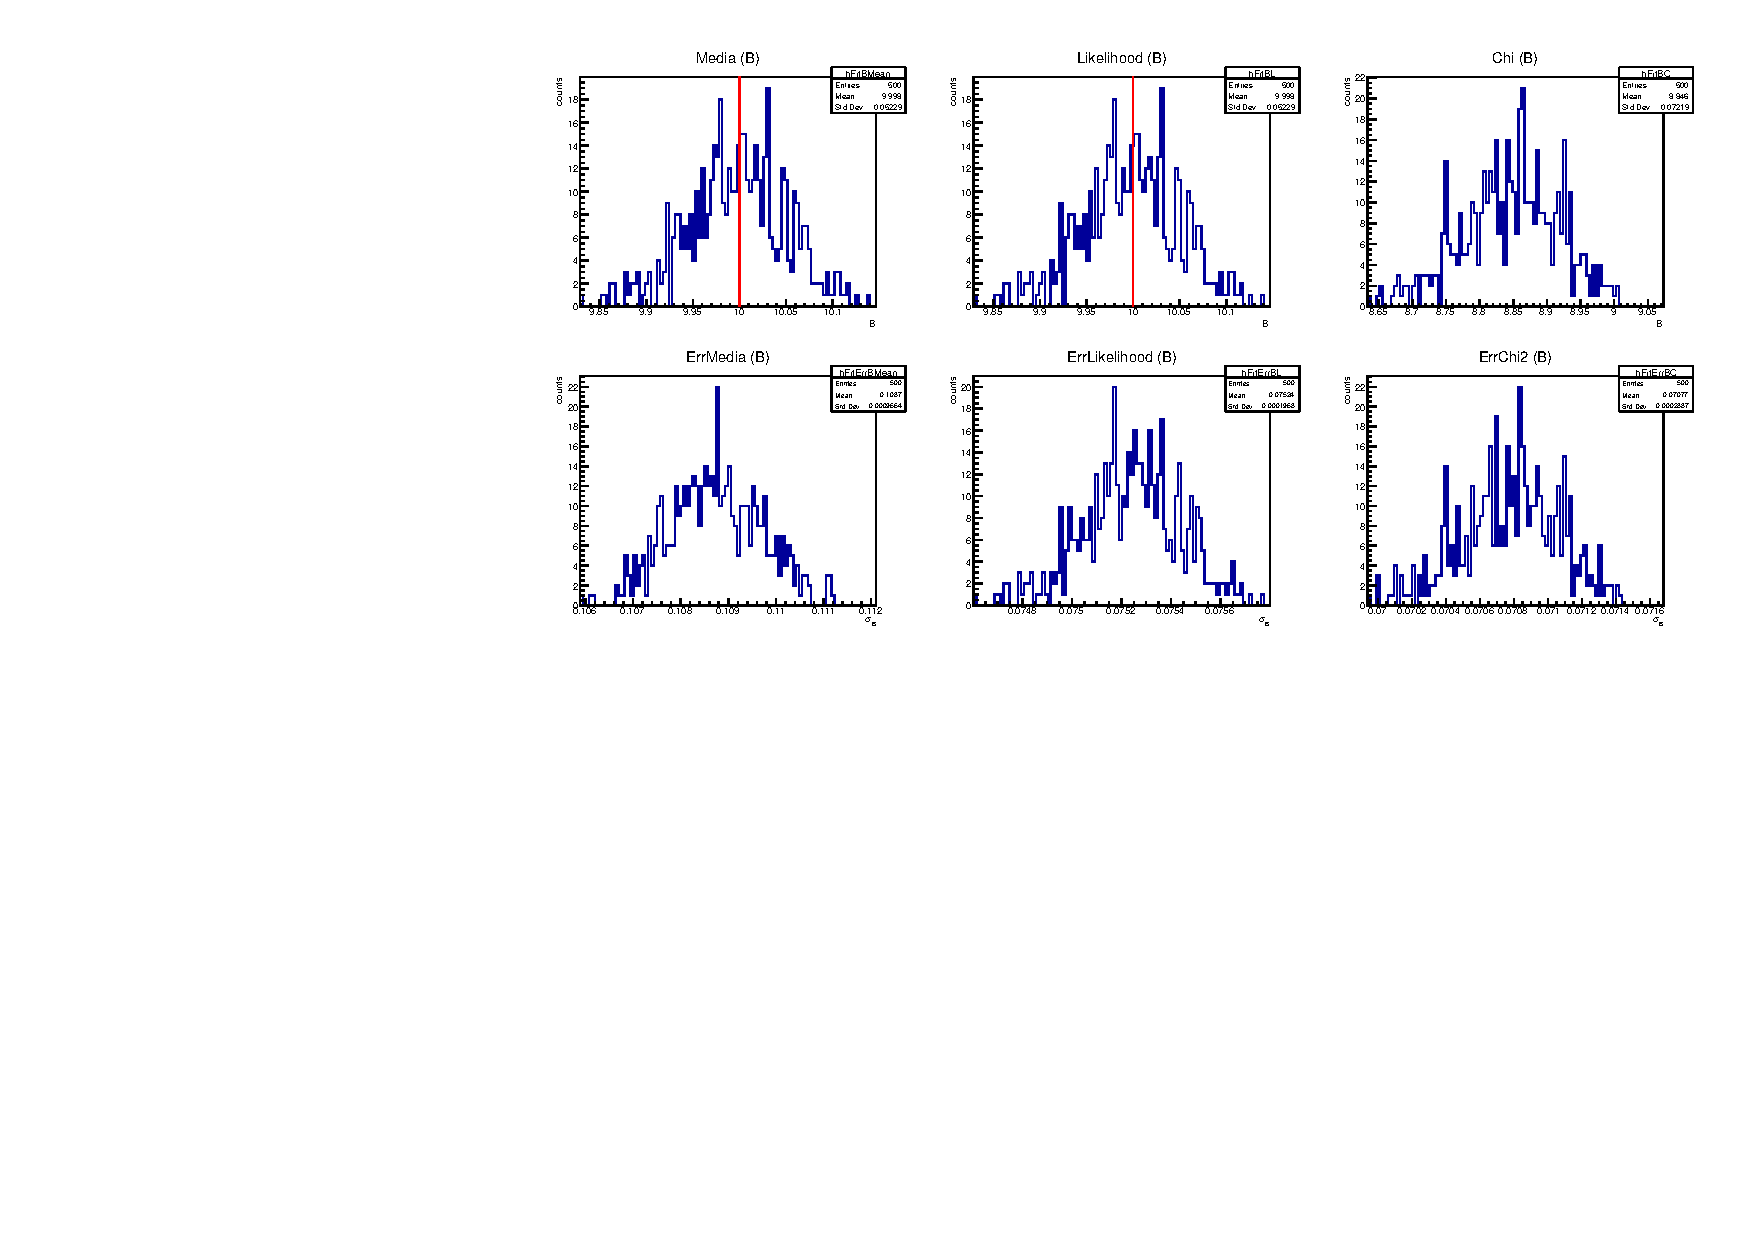
\includegraphics[scale=0.75]{img/baseline_sim_500.pdf}}
 \end{adjustbox}}
 \caption{Distribuzioni delle stime della \textit{baseline} con i tre metodi differenti, sia per i valori sia per gli errori (500 simulazioni). La \textit{baseline} generata in queste simulazioni ha altezza 10.}\label{fig::baseline_500}
\end{figure}
%
In figura \ref{fig::baseline_500} è riportato un esempio delle distribuzioni dei valori e degli errori derivanti da simulazioni multiple, stimati con i tre metodi. La linea rossa verticale nei grafici in alto indica il valore vero della \textit{baseline}, ossia il valore con cui sono stati simulati gli spettri, quindi il valore che dovrebbe essere restituito dall'analisi. Come si può notare, la distribuzione dei valori estratta con fit \lstinline{pol0} di tipo $\chi^2$ non è centrata attorno al valore atteso. In questo caso, infatti, la baseline è sistematicamente sottostimata, poichè:
\begin{enumerate}
 \item il metodo dei minimi quadrati non funziona correttamente per il fit di un istogramma con bin a bassa statistica, per i quali l'assegnazione di errore di tipo poissoniano (cioè la radice del conteggio) presenta delle criticità, in particolare per contenuti nulli;
 \item il fit di una \lstinline{pol0} con il metodo del $\chi^2$ corrisponde esattamente ad una media pesata, nella quale i bin con statistica minore hanno un peso maggiore, con conseguenti valori sottostimati della \textit{baseline}\footnote{Media pesata ed errore:
$$\bar{b}=\frac{\sum_{i=1}^N b_i/\sigma_i^2}{\sum_{i=1}^N 1/\sigma_i^2};
\hspace{1cm} \sigma_{\bar{b}}=\frac{1}{\sum_{i=1}^N1/\sigma_i^2}$$}.
 
\end{enumerate}
In virtù di queste considerazioni, il metodo di fit del $\chi^2$ è stato dunque scartato. 
Gli spettri relativi agli errori statistici sulla \textit{baseline} sono utili per controllare che le distribuzioni dei valori non siano troppo disperse. In altre parole, si effettua il confronto tra la $\sigma$ delle gaussiane dei valori e il centroide $\overline{\sigma_{b}}$ delle gaussiane degli errori, controllando che $\sigma\lesssim \overline{\sigma_{b}}$, condizione soddisfatta nelle simulazioni in esame.
%
\subsection{Simulazione del fondo e del primo esponenziale}
Una seconda versione del Metodo Montecarlo prevede di studiare una distribuzione contenente un termine costante e un termine esponenziale. 
\begin{equation}
 f(t;A,\tau,b)=Ae^{-\frac{t}{\tau}}+b
 \label{eq::exp_plus_base}
\end{equation}
Per la costruzione delle distribuzioni si è scelto di generare indipendentemente la distribuzione uniforme con \lstinline{TRandom3::Uniform} e la distribuzione esponenziale con \lstinline{TRandom3::Exp} per poi sommarle. Avendo stabilito che il metodo della maximum likelihood è il più stabile e predittivo si sono studiati diversi approcci al fit della distribuzione:
\begin{enumerate}
  \item Fit diretto con la funzione completa impostando $\tau$ al valore vero e lasciando $A$ e $b$ non inizializzati;
  \item Fit di tipo \lstinline{pol0} della parte finale dello spettro per la stima di $b$, utilizzata in secondo luogo per inizializzare il corrispondente parametro nel fit con la funzione completa del metodo precedente;
  \item Fit di tipo \lstinline{pol0} della parte finale dello spettro per la stima di $b$, quindi sottrazione della componente costante della distribuzione e successivo fit puramente esponenziale.
\end{enumerate}
Dei tre metodi il secondo si è rivelato il più stabile; un fit a tre parametri, infatti, necessita di valori di partenza che siano sufficientemente vicini al valore vero affinchè l'algoritmo di massimizzazione della likelihood vada a convergenza correttamente, e ciò ci porta a scartare il primo metodo, poco stabile con valori iniziali distanti dal valore vero. Anche il terzo metodo presenta delle criticità aggiuntive rispetto al secondo: in primo luogo una sottrazione di dati a bassa statistica può facilmente portare ad avere canali a contenuto negativo (privo di significato fisico), in secondo luogo, come si può notare dalla figura \ref{baselinestart}, il fit della \textit{baseline} sovrastima il valore di $b$ e perciò la sottrazione non può essere considerata corretta.

L'adozione del secondo metodo richiede la scelta del canale (valore di ritardo temporale) dal quale far iniziare il fit della porzione di \textit{baseline}, si è quindi proceduto a eseguire uno studio sistematico dei risultati al variare di questo estremo inferiore confrontando le medie su più simulazioni (figura \ref{baselinestart}). Dal grafico è evidente come la riscostruzione sia più precisa ma meno accurata per piccoli valori e di come la situazione si inverta per grandi valori. A priori si potrebbe scegliere un valore che rappresenti la media tra queste due situazioni, ma a posteriori, studiando la ricostruzione di $b$ e $\tau^+$ dopo il fit esponenziale del metodo 2, si è verificato con varie prove come la scelta di questo valore iniziale sia del tutto ininfluente.
%
\begin{figure}[h]
  \centerline{%
  \begin{adjustbox}{width=\linewidth+1cm}
    \begin{tikzpicture}
\pgfdeclareplotmark{cross} {
\pgfpathmoveto{\pgfpoint{-0.3\pgfplotmarksize}{\pgfplotmarksize}}
\pgfpathlineto{\pgfpoint{+0.3\pgfplotmarksize}{\pgfplotmarksize}}
\pgfpathlineto{\pgfpoint{+0.3\pgfplotmarksize}{0.3\pgfplotmarksize}}
\pgfpathlineto{\pgfpoint{+1\pgfplotmarksize}{0.3\pgfplotmarksize}}
\pgfpathlineto{\pgfpoint{+1\pgfplotmarksize}{-0.3\pgfplotmarksize}}
\pgfpathlineto{\pgfpoint{+0.3\pgfplotmarksize}{-0.3\pgfplotmarksize}}
\pgfpathlineto{\pgfpoint{+0.3\pgfplotmarksize}{-1.\pgfplotmarksize}}
\pgfpathlineto{\pgfpoint{-0.3\pgfplotmarksize}{-1.\pgfplotmarksize}}
\pgfpathlineto{\pgfpoint{-0.3\pgfplotmarksize}{-0.3\pgfplotmarksize}}
\pgfpathlineto{\pgfpoint{-1.\pgfplotmarksize}{-0.3\pgfplotmarksize}}
\pgfpathlineto{\pgfpoint{-1.\pgfplotmarksize}{0.3\pgfplotmarksize}}
\pgfpathlineto{\pgfpoint{-0.3\pgfplotmarksize}{0.3\pgfplotmarksize}}
\pgfpathclose
\pgfusepathqstroke
}
\pgfdeclareplotmark{cross*} {
\pgfpathmoveto{\pgfpoint{-0.3\pgfplotmarksize}{\pgfplotmarksize}}
\pgfpathlineto{\pgfpoint{+0.3\pgfplotmarksize}{\pgfplotmarksize}}
\pgfpathlineto{\pgfpoint{+0.3\pgfplotmarksize}{0.3\pgfplotmarksize}}
\pgfpathlineto{\pgfpoint{+1\pgfplotmarksize}{0.3\pgfplotmarksize}}
\pgfpathlineto{\pgfpoint{+1\pgfplotmarksize}{-0.3\pgfplotmarksize}}
\pgfpathlineto{\pgfpoint{+0.3\pgfplotmarksize}{-0.3\pgfplotmarksize}}
\pgfpathlineto{\pgfpoint{+0.3\pgfplotmarksize}{-1.\pgfplotmarksize}}
\pgfpathlineto{\pgfpoint{-0.3\pgfplotmarksize}{-1.\pgfplotmarksize}}
\pgfpathlineto{\pgfpoint{-0.3\pgfplotmarksize}{-0.3\pgfplotmarksize}}
\pgfpathlineto{\pgfpoint{-1.\pgfplotmarksize}{-0.3\pgfplotmarksize}}
\pgfpathlineto{\pgfpoint{-1.\pgfplotmarksize}{0.3\pgfplotmarksize}}
\pgfpathlineto{\pgfpoint{-0.3\pgfplotmarksize}{0.3\pgfplotmarksize}}
\pgfpathclose
\pgfusepathqfillstroke
}
\pgfdeclareplotmark{newstar} {
\pgfpathmoveto{\pgfqpoint{0pt}{\pgfplotmarksize}}
\pgfpathlineto{\pgfqpointpolar{44}{0.5\pgfplotmarksize}}
\pgfpathlineto{\pgfqpointpolar{18}{\pgfplotmarksize}}
\pgfpathlineto{\pgfqpointpolar{-20}{0.5\pgfplotmarksize}}
\pgfpathlineto{\pgfqpointpolar{-54}{\pgfplotmarksize}}
\pgfpathlineto{\pgfqpointpolar{-90}{0.5\pgfplotmarksize}}
\pgfpathlineto{\pgfqpointpolar{234}{\pgfplotmarksize}}
\pgfpathlineto{\pgfqpointpolar{198}{0.5\pgfplotmarksize}}
\pgfpathlineto{\pgfqpointpolar{162}{\pgfplotmarksize}}
\pgfpathlineto{\pgfqpointpolar{134}{0.5\pgfplotmarksize}}
\pgfpathclose
\pgfusepathqstroke
}
\pgfdeclareplotmark{newstar*} {
\pgfpathmoveto{\pgfqpoint{0pt}{\pgfplotmarksize}}
\pgfpathlineto{\pgfqpointpolar{44}{0.5\pgfplotmarksize}}
\pgfpathlineto{\pgfqpointpolar{18}{\pgfplotmarksize}}
\pgfpathlineto{\pgfqpointpolar{-20}{0.5\pgfplotmarksize}}
\pgfpathlineto{\pgfqpointpolar{-54}{\pgfplotmarksize}}
\pgfpathlineto{\pgfqpointpolar{-90}{0.5\pgfplotmarksize}}
\pgfpathlineto{\pgfqpointpolar{234}{\pgfplotmarksize}}
\pgfpathlineto{\pgfqpointpolar{198}{0.5\pgfplotmarksize}}
\pgfpathlineto{\pgfqpointpolar{162}{\pgfplotmarksize}}
\pgfpathlineto{\pgfqpointpolar{134}{0.5\pgfplotmarksize}}
\pgfpathclose
\pgfusepathqfillstroke
}
\definecolor{c}{rgb}{1,1,1};
\draw [color=c, fill=c] (0,0) rectangle (20,13.0092);
\draw [color=c, fill=c] (0.197109,6.64915) rectangle (19.6189,12.9041);
\draw [color=c, fill=c] (1.76084,7.43758) rectangle (19.0013,12.2996);
\definecolor{c}{rgb}{0,0,0};
\draw [c,line width=0.9] (1.76084,7.43758) -- (1.76084,12.2996) -- (19.0013,12.2996) -- (19.0013,7.43758) -- (1.76084,7.43758);
\definecolor{c}{rgb}{1,1,1};
\draw [color=c, fill=c] (1.76084,7.43758) rectangle (19.0013,12.2996);
\definecolor{c}{rgb}{0,0,0};
\draw [c,line width=0.9] (1.76084,7.43758) -- (1.76084,12.2996) -- (19.0013,12.2996) -- (19.0013,7.43758) -- (1.76084,7.43758);
\draw [c,line width=0.9] (1.76084,7.43758) -- (19.0013,7.43758);
\draw [c,dash pattern=on 0.80pt off 1.60pt ,line width=0.9] (2.2953,12.2996) -- (2.2953,7.43758);
\draw [c,dash pattern=on 0.80pt off 1.60pt ,line width=0.9] (4.01934,12.2996) -- (4.01934,7.43758);
\draw [c,dash pattern=on 0.80pt off 1.60pt ,line width=0.9] (5.74339,12.2996) -- (5.74339,7.43758);
\draw [c,dash pattern=on 0.80pt off 1.60pt ,line width=0.9] (7.46744,12.2996) -- (7.46744,7.43758);
\draw [c,dash pattern=on 0.80pt off 1.60pt ,line width=0.9] (9.19148,12.2996) -- (9.19148,7.43758);
\draw [c,dash pattern=on 0.80pt off 1.60pt ,line width=0.9] (10.9155,12.2996) -- (10.9155,7.43758);
\draw [c,dash pattern=on 0.80pt off 1.60pt ,line width=0.9] (12.6396,12.2996) -- (12.6396,7.43758);
\draw [c,dash pattern=on 0.80pt off 1.60pt ,line width=0.9] (14.3636,12.2996) -- (14.3636,7.43758);
\draw [c,dash pattern=on 0.80pt off 1.60pt ,line width=0.9] (16.0877,12.2996) -- (16.0877,7.43758);
\draw [c,dash pattern=on 0.80pt off 1.60pt ,line width=0.9] (17.8117,12.2996) -- (17.8117,7.43758);
\draw [c,dash pattern=on 0.80pt off 1.60pt ,line width=0.9] (2.2953,12.2996) -- (2.2953,7.43758);
\draw [c,dash pattern=on 0.80pt off 1.60pt ,line width=0.9] (17.8117,12.2996) -- (17.8117,7.43758);
\draw [c,line width=0.9] (1.76084,7.43758) -- (1.76084,12.2996);
\draw [c,dash pattern=on 0.80pt off 1.60pt ,line width=0.9] (19.0013,7.43758) -- (1.76084,7.43758);
\draw [c,dash pattern=on 0.80pt off 1.60pt ,line width=0.9] (19.0013,7.93174) -- (1.76084,7.93174);
\draw [c,dash pattern=on 0.80pt off 1.60pt ,line width=0.9] (19.0013,8.4259) -- (1.76084,8.4259);
\draw [c,dash pattern=on 0.80pt off 1.60pt ,line width=0.9] (19.0013,8.92006) -- (1.76084,8.92006);
\draw [c,dash pattern=on 0.80pt off 1.60pt ,line width=0.9] (19.0013,9.41422) -- (1.76084,9.41422);
\draw [c,dash pattern=on 0.80pt off 1.60pt ,line width=0.9] (19.0013,9.90838) -- (1.76084,9.90838);
\draw [c,dash pattern=on 0.80pt off 1.60pt ,line width=0.9] (19.0013,10.4025) -- (1.76084,10.4025);
\draw [c,dash pattern=on 0.80pt off 1.60pt ,line width=0.9] (19.0013,10.8967) -- (1.76084,10.8967);
\draw [c,dash pattern=on 0.80pt off 1.60pt ,line width=0.9] (19.0013,11.3909) -- (1.76084,11.3909);
\draw [c,dash pattern=on 0.80pt off 1.60pt ,line width=0.9] (19.0013,11.885) -- (1.76084,11.885);
\draw [c,dash pattern=on 0.80pt off 1.60pt ,line width=0.9] (19.0013,11.885) -- (1.76084,11.885);
\definecolor{c}{rgb}{0,0,0.6};
\draw [c,line width=0.9] (1.76515,11.8559) -- (1.76515,11.962);
\draw [c,line width=0.9] (1.76515,11.962) -- (1.76515,12.0681);
\draw [c,line width=0.9] (1.76084,11.962) -- (1.76515,11.962);
\draw [c,line width=0.9] (1.76515,11.962) -- (1.76946,11.962);
\draw [c,line width=0.9] (1.71259,11.8559) -- (1.81771,11.8559);
\draw [c,line width=0.9] (1.71259,12.0681) -- (1.81771,12.0681);
\draw [c,line width=0.9] (1.76084,11.9094) -- (1.76084,12.0146);
\draw [c,line width=0.9] (1.76946,11.9094) -- (1.76946,12.0146);
\definecolor{c}{rgb}{0,0,0};
\foreach \P in {(1.76515,11.962)}{\draw[mark options={color=c,fill=c},mark size=2.402402pt,mark=*,mark size=1pt] plot coordinates {\P};}
\definecolor{c}{rgb}{0,0,0.6};
\draw [c,line width=0.9] (2.33409,11.4287) -- (2.33409,11.5349);
\draw [c,line width=0.9] (2.33409,11.5349) -- (2.33409,11.6411);
\draw [c,line width=0.9] (2.32978,11.5349) -- (2.33409,11.5349);
\draw [c,line width=0.9] (2.33409,11.5349) -- (2.3384,11.5349);
\draw [c,line width=0.9] (2.28152,11.4287) -- (2.38665,11.4287);
\draw [c,line width=0.9] (2.28152,11.6411) -- (2.38665,11.6411);
\draw [c,line width=0.9] (2.32978,11.4824) -- (2.32978,11.5875);
\draw [c,line width=0.9] (2.3384,11.4824) -- (2.3384,11.5875);
\definecolor{c}{rgb}{0,0,0};
\foreach \P in {(2.33409,11.5349)}{\draw[mark options={color=c,fill=c},mark size=2.402402pt,mark=*,mark size=1pt] plot coordinates {\P};}
\definecolor{c}{rgb}{0,0,0.6};
\draw [c,line width=0.9] (2.90302,11.0641) -- (2.90302,11.1606);
\draw [c,line width=0.9] (2.90302,11.1606) -- (2.90302,11.257);
\draw [c,line width=0.9] (2.89871,11.1606) -- (2.90302,11.1606);
\draw [c,line width=0.9] (2.90302,11.1606) -- (2.90733,11.1606);
\draw [c,line width=0.9] (2.85046,11.0641) -- (2.95558,11.0641);
\draw [c,line width=0.9] (2.85046,11.257) -- (2.95558,11.257);
\draw [c,line width=0.9] (2.89871,11.108) -- (2.89871,11.2131);
\draw [c,line width=0.9] (2.90733,11.108) -- (2.90733,11.2131);
\definecolor{c}{rgb}{0,0,0};
\foreach \P in {(2.90302,11.1606)}{\draw[mark options={color=c,fill=c},mark size=2.402402pt,mark=*,mark size=1pt] plot coordinates {\P};}
\definecolor{c}{rgb}{0,0,0.6};
\draw [c,line width=0.9] (3.47196,10.7466) -- (3.47196,10.8316);
\draw [c,line width=0.9] (3.47196,10.8316) -- (3.47196,10.9167);
\draw [c,line width=0.9] (3.46765,10.8316) -- (3.47196,10.8316);
\draw [c,line width=0.9] (3.47196,10.8316) -- (3.47627,10.8316);
\draw [c,line width=0.9] (3.4194,10.7466) -- (3.52452,10.7466);
\draw [c,line width=0.9] (3.4194,10.9167) -- (3.52452,10.9167);
\draw [c,line width=0.9] (3.46765,10.7791) -- (3.46765,10.8842);
\draw [c,line width=0.9] (3.47627,10.7791) -- (3.47627,10.8842);
\definecolor{c}{rgb}{0,0,0};
\foreach \P in {(3.47196,10.8316)}{\draw[mark options={color=c,fill=c},mark size=2.402402pt,mark=*,mark size=1pt] plot coordinates {\P};}
\definecolor{c}{rgb}{0,0,0.6};
\draw [c,line width=0.9] (4.04089,10.4778) -- (4.04089,10.5565);
\draw [c,line width=0.9] (4.04089,10.5565) -- (4.04089,10.6353);
\draw [c,line width=0.9] (4.03658,10.5565) -- (4.04089,10.5565);
\draw [c,line width=0.9] (4.04089,10.5565) -- (4.0452,10.5565);
\draw [c,line width=0.9] (3.98833,10.4778) -- (4.09346,10.4778);
\draw [c,line width=0.9] (3.98833,10.6353) -- (4.09346,10.6353);
\draw [c,line width=0.9] (4.03658,10.504) -- (4.03658,10.6091);
\draw [c,line width=0.9] (4.0452,10.504) -- (4.0452,10.6091);
\definecolor{c}{rgb}{0,0,0};
\foreach \P in {(4.04089,10.5565)}{\draw[mark options={color=c,fill=c},mark size=2.402402pt,mark=*,mark size=1pt] plot coordinates {\P};}
\definecolor{c}{rgb}{0,0,0.6};
\draw [c,line width=0.9] (4.60983,10.2184) -- (4.60983,10.297);
\draw [c,line width=0.9] (4.60983,10.297) -- (4.60983,10.3755);
\draw [c,line width=0.9] (4.60552,10.297) -- (4.60983,10.297);
\draw [c,line width=0.9] (4.60983,10.297) -- (4.61414,10.297);
\draw [c,line width=0.9] (4.55727,10.2184) -- (4.66239,10.2184);
\draw [c,line width=0.9] (4.55727,10.3755) -- (4.66239,10.3755);
\draw [c,line width=0.9] (4.60552,10.2444) -- (4.60552,10.3495);
\draw [c,line width=0.9] (4.61414,10.2444) -- (4.61414,10.3495);
\definecolor{c}{rgb}{0,0,0};
\foreach \P in {(4.60983,10.297)}{\draw[mark options={color=c,fill=c},mark size=2.402402pt,mark=*,mark size=1pt] plot coordinates {\P};}
\definecolor{c}{rgb}{0,0,0.6};
\draw [c,line width=0.9] (5.17876,9.99563) -- (5.17876,10.0852);
\draw [c,line width=0.9] (5.17876,10.0852) -- (5.17876,10.1748);
\draw [c,line width=0.9] (5.17445,10.0852) -- (5.17876,10.0852);
\draw [c,line width=0.9] (5.17876,10.0852) -- (5.18307,10.0852);
\draw [c,line width=0.9] (5.1262,9.99563) -- (5.23133,9.99563);
\draw [c,line width=0.9] (5.1262,10.1748) -- (5.23133,10.1748);
\draw [c,line width=0.9] (5.17445,10.0326) -- (5.17445,10.1378);
\draw [c,line width=0.9] (5.18307,10.0326) -- (5.18307,10.1378);
\definecolor{c}{rgb}{0,0,0};
\foreach \P in {(5.17876,10.0852)}{\draw[mark options={color=c,fill=c},mark size=2.402402pt,mark=*,mark size=1pt] plot coordinates {\P};}
\definecolor{c}{rgb}{0,0,0.6};
\draw [c,line width=0.9] (5.7477,9.81474) -- (5.7477,9.89912);
\draw [c,line width=0.9] (5.7477,9.89912) -- (5.7477,9.9835);
\draw [c,line width=0.9] (5.74339,9.89912) -- (5.7477,9.89912);
\draw [c,line width=0.9] (5.7477,9.89912) -- (5.75201,9.89912);
\draw [c,line width=0.9] (5.69514,9.81474) -- (5.80026,9.81474);
\draw [c,line width=0.9] (5.69514,9.9835) -- (5.80026,9.9835);
\draw [c,line width=0.9] (5.74339,9.84656) -- (5.74339,9.95168);
\draw [c,line width=0.9] (5.75201,9.84656) -- (5.75201,9.95168);
\definecolor{c}{rgb}{0,0,0};
\foreach \P in {(5.7477,9.89912)}{\draw[mark options={color=c,fill=c},mark size=2.402402pt,mark=*,mark size=1pt] plot coordinates {\P};}
\definecolor{c}{rgb}{0,0,0.6};
\draw [c,line width=0.9] (6.31664,9.64435) -- (6.31664,9.72887);
\draw [c,line width=0.9] (6.31664,9.72887) -- (6.31664,9.81339);
\draw [c,line width=0.9] (6.31233,9.72887) -- (6.31664,9.72887);
\draw [c,line width=0.9] (6.31664,9.72887) -- (6.32095,9.72887);
\draw [c,line width=0.9] (6.26407,9.64435) -- (6.3692,9.64435);
\draw [c,line width=0.9] (6.26407,9.81339) -- (6.3692,9.81339);
\draw [c,line width=0.9] (6.31233,9.67631) -- (6.31233,9.78143);
\draw [c,line width=0.9] (6.32095,9.67631) -- (6.32095,9.78143);
\definecolor{c}{rgb}{0,0,0};
\foreach \P in {(6.31664,9.72887)}{\draw[mark options={color=c,fill=c},mark size=2.402402pt,mark=*,mark size=1pt] plot coordinates {\P};}
\definecolor{c}{rgb}{0,0,0.6};
\draw [c,line width=0.9] (6.88557,9.49105) -- (6.88557,9.58247);
\draw [c,line width=0.9] (6.88557,9.58247) -- (6.88557,9.6739);
\draw [c,line width=0.9] (6.88126,9.58247) -- (6.88557,9.58247);
\draw [c,line width=0.9] (6.88557,9.58247) -- (6.88988,9.58247);
\draw [c,line width=0.9] (6.83301,9.49105) -- (6.93813,9.49105);
\draw [c,line width=0.9] (6.83301,9.6739) -- (6.93813,9.6739);
\draw [c,line width=0.9] (6.88126,9.52991) -- (6.88126,9.63504);
\draw [c,line width=0.9] (6.88988,9.52991) -- (6.88988,9.63504);
\definecolor{c}{rgb}{0,0,0};
\foreach \P in {(6.88557,9.58247)}{\draw[mark options={color=c,fill=c},mark size=2.402402pt,mark=*,mark size=1pt] plot coordinates {\P};}
\definecolor{c}{rgb}{0,0,0.6};
\draw [c,line width=0.9] (7.45451,9.35429) -- (7.45451,9.4567);
\draw [c,line width=0.9] (7.45451,9.4567) -- (7.45451,9.5591);
\draw [c,line width=0.9] (7.4502,9.4567) -- (7.45451,9.4567);
\draw [c,line width=0.9] (7.45451,9.4567) -- (7.45882,9.4567);
\draw [c,line width=0.9] (7.40194,9.35429) -- (7.50707,9.35429);
\draw [c,line width=0.9] (7.40194,9.5591) -- (7.50707,9.5591);
\draw [c,line width=0.9] (7.4502,9.40414) -- (7.4502,9.50926);
\draw [c,line width=0.9] (7.45882,9.40414) -- (7.45882,9.50926);
\definecolor{c}{rgb}{0,0,0};
\foreach \P in {(7.45451,9.4567)}{\draw[mark options={color=c,fill=c},mark size=2.402402pt,mark=*,mark size=1pt] plot coordinates {\P};}
\definecolor{c}{rgb}{0,0,0.6};
\draw [c,line width=0.9] (8.02344,9.23709) -- (8.02344,9.34039);
\draw [c,line width=0.9] (8.02344,9.34039) -- (8.02344,9.44369);
\draw [c,line width=0.9] (8.01913,9.34039) -- (8.02344,9.34039);
\draw [c,line width=0.9] (8.02344,9.34039) -- (8.02775,9.34039);
\draw [c,line width=0.9] (7.97088,9.23709) -- (8.076,9.23709);
\draw [c,line width=0.9] (7.97088,9.44369) -- (8.076,9.44369);
\draw [c,line width=0.9] (8.01913,9.28783) -- (8.01913,9.39295);
\draw [c,line width=0.9] (8.02775,9.28783) -- (8.02775,9.39295);
\definecolor{c}{rgb}{0,0,0};
\foreach \P in {(8.02344,9.34039)}{\draw[mark options={color=c,fill=c},mark size=2.402402pt,mark=*,mark size=1pt] plot coordinates {\P};}
\definecolor{c}{rgb}{0,0,0.6};
\draw [c,line width=0.9] (8.59238,9.13913) -- (8.59238,9.23286);
\draw [c,line width=0.9] (8.59238,9.23286) -- (8.59238,9.3266);
\draw [c,line width=0.9] (8.58807,9.23286) -- (8.59238,9.23286);
\draw [c,line width=0.9] (8.59238,9.23286) -- (8.59669,9.23286);
\draw [c,line width=0.9] (8.53982,9.13913) -- (8.64494,9.13913);
\draw [c,line width=0.9] (8.53982,9.3266) -- (8.64494,9.3266);
\draw [c,line width=0.9] (8.58807,9.1803) -- (8.58807,9.28543);
\draw [c,line width=0.9] (8.59669,9.1803) -- (8.59669,9.28543);
\definecolor{c}{rgb}{0,0,0};
\foreach \P in {(8.59238,9.23286)}{\draw[mark options={color=c,fill=c},mark size=2.402402pt,mark=*,mark size=1pt] plot coordinates {\P};}
\definecolor{c}{rgb}{0,0,0.6};
\draw [c,line width=0.9] (9.16131,9.05208) -- (9.16131,9.14867);
\draw [c,line width=0.9] (9.16131,9.14867) -- (9.16131,9.24526);
\draw [c,line width=0.9] (9.157,9.14867) -- (9.16131,9.14867);
\draw [c,line width=0.9] (9.16131,9.14867) -- (9.16562,9.14867);
\draw [c,line width=0.9] (9.10875,9.05208) -- (9.21388,9.05208);
\draw [c,line width=0.9] (9.10875,9.24526) -- (9.21388,9.24526);
\draw [c,line width=0.9] (9.157,9.09611) -- (9.157,9.20123);
\draw [c,line width=0.9] (9.16562,9.09611) -- (9.16562,9.20123);
\definecolor{c}{rgb}{0,0,0};
\foreach \P in {(9.16131,9.14867)}{\draw[mark options={color=c,fill=c},mark size=2.402402pt,mark=*,mark size=1pt] plot coordinates {\P};}
\definecolor{c}{rgb}{0,0,0.6};
\draw [c,line width=0.9] (9.73025,8.97208) -- (9.73025,9.06787);
\draw [c,line width=0.9] (9.73025,9.06787) -- (9.73025,9.16365);
\draw [c,line width=0.9] (9.72594,9.06787) -- (9.73025,9.06787);
\draw [c,line width=0.9] (9.73025,9.06787) -- (9.73456,9.06787);
\draw [c,line width=0.9] (9.67769,8.97208) -- (9.78281,8.97208);
\draw [c,line width=0.9] (9.67769,9.16365) -- (9.78281,9.16365);
\draw [c,line width=0.9] (9.72594,9.0153) -- (9.72594,9.12043);
\draw [c,line width=0.9] (9.73456,9.0153) -- (9.73456,9.12043);
\definecolor{c}{rgb}{0,0,0};
\foreach \P in {(9.73025,9.06787)}{\draw[mark options={color=c,fill=c},mark size=2.402402pt,mark=*,mark size=1pt] plot coordinates {\P};}
\definecolor{c}{rgb}{0,0,0.6};
\draw [c,line width=0.9] (10.2992,8.88708) -- (10.2992,8.98708);
\draw [c,line width=0.9] (10.2992,8.98708) -- (10.2992,9.08707);
\draw [c,line width=0.9] (10.2949,8.98708) -- (10.2992,8.98708);
\draw [c,line width=0.9] (10.2992,8.98708) -- (10.3035,8.98708);
\draw [c,line width=0.9] (10.2466,8.88708) -- (10.3517,8.88708);
\draw [c,line width=0.9] (10.2466,9.08707) -- (10.3517,9.08707);
\draw [c,line width=0.9] (10.2949,8.93452) -- (10.2949,9.03964);
\draw [c,line width=0.9] (10.3035,8.93452) -- (10.3035,9.03964);
\definecolor{c}{rgb}{0,0,0};
\foreach \P in {(10.2992,8.98708)}{\draw[mark options={color=c,fill=c},mark size=2.402402pt,mark=*,mark size=1pt] plot coordinates {\P};}
\definecolor{c}{rgb}{0,0,0.6};
\draw [c,line width=0.9] (10.8681,8.81572) -- (10.8681,8.92722);
\draw [c,line width=0.9] (10.8681,8.92722) -- (10.8681,9.03872);
\draw [c,line width=0.9] (10.8638,8.92722) -- (10.8681,8.92722);
\draw [c,line width=0.9] (10.8681,8.92722) -- (10.8724,8.92722);
\draw [c,line width=0.9] (10.8156,8.81572) -- (10.9207,8.81572);
\draw [c,line width=0.9] (10.8156,9.03872) -- (10.9207,9.03872);
\draw [c,line width=0.9] (10.8638,8.87466) -- (10.8638,8.97978);
\draw [c,line width=0.9] (10.8724,8.87466) -- (10.8724,8.97978);
\definecolor{c}{rgb}{0,0,0};
\foreach \P in {(10.8681,8.92722)}{\draw[mark options={color=c,fill=c},mark size=2.402402pt,mark=*,mark size=1pt] plot coordinates {\P};}
\definecolor{c}{rgb}{0,0,0.6};
\draw [c,line width=0.9] (11.4371,8.76513) -- (11.4371,8.87623);
\draw [c,line width=0.9] (11.4371,8.87623) -- (11.4371,8.98733);
\draw [c,line width=0.9] (11.4327,8.87623) -- (11.4371,8.87623);
\draw [c,line width=0.9] (11.4371,8.87623) -- (11.4414,8.87623);
\draw [c,line width=0.9] (11.3845,8.76513) -- (11.4896,8.76513);
\draw [c,line width=0.9] (11.3845,8.98733) -- (11.4896,8.98733);
\draw [c,line width=0.9] (11.4327,8.82367) -- (11.4327,8.92879);
\draw [c,line width=0.9] (11.4414,8.82367) -- (11.4414,8.92879);
\definecolor{c}{rgb}{0,0,0};
\foreach \P in {(11.4371,8.87623)}{\draw[mark options={color=c,fill=c},mark size=2.402402pt,mark=*,mark size=1pt] plot coordinates {\P};}
\definecolor{c}{rgb}{0,0,0.6};
\draw [c,line width=0.9] (12.006,8.68691) -- (12.006,8.82007);
\draw [c,line width=0.9] (12.006,8.82007) -- (12.006,8.95324);
\draw [c,line width=0.9] (12.0017,8.82007) -- (12.006,8.82007);
\draw [c,line width=0.9] (12.006,8.82007) -- (12.0103,8.82007);
\draw [c,line width=0.9] (11.9534,8.68691) -- (12.0586,8.68691);
\draw [c,line width=0.9] (11.9534,8.95324) -- (12.0586,8.95324);
\draw [c,line width=0.9] (12.0017,8.76751) -- (12.0017,8.87264);
\draw [c,line width=0.9] (12.0103,8.76751) -- (12.0103,8.87264);
\definecolor{c}{rgb}{0,0,0};
\foreach \P in {(12.006,8.82007)}{\draw[mark options={color=c,fill=c},mark size=2.402402pt,mark=*,mark size=1pt] plot coordinates {\P};}
\definecolor{c}{rgb}{0,0,0.6};
\draw [c,line width=0.9] (12.5749,8.65095) -- (12.5749,8.78791);
\draw [c,line width=0.9] (12.5749,8.78791) -- (12.5749,8.92487);
\draw [c,line width=0.9] (12.5706,8.78791) -- (12.5749,8.78791);
\draw [c,line width=0.9] (12.5749,8.78791) -- (12.5792,8.78791);
\draw [c,line width=0.9] (12.5224,8.65095) -- (12.6275,8.65095);
\draw [c,line width=0.9] (12.5224,8.92487) -- (12.6275,8.92487);
\draw [c,line width=0.9] (12.5706,8.73535) -- (12.5706,8.84047);
\draw [c,line width=0.9] (12.5792,8.73535) -- (12.5792,8.84047);
\definecolor{c}{rgb}{0,0,0};
\foreach \P in {(12.5749,8.78791)}{\draw[mark options={color=c,fill=c},mark size=2.402402pt,mark=*,mark size=1pt] plot coordinates {\P};}
\definecolor{c}{rgb}{0,0,0.6};
\draw [c,line width=0.9] (13.1439,8.61429) -- (13.1439,8.7547);
\draw [c,line width=0.9] (13.1439,8.7547) -- (13.1439,8.8951);
\draw [c,line width=0.9] (13.1396,8.7547) -- (13.1439,8.7547);
\draw [c,line width=0.9] (13.1439,8.7547) -- (13.1482,8.7547);
\draw [c,line width=0.9] (13.0913,8.61429) -- (13.1964,8.61429);
\draw [c,line width=0.9] (13.0913,8.8951) -- (13.1964,8.8951);
\draw [c,line width=0.9] (13.1396,8.70213) -- (13.1396,8.80726);
\draw [c,line width=0.9] (13.1482,8.70213) -- (13.1482,8.80726);
\definecolor{c}{rgb}{0,0,0};
\foreach \P in {(13.1439,8.7547)}{\draw[mark options={color=c,fill=c},mark size=2.402402pt,mark=*,mark size=1pt] plot coordinates {\P};}
\definecolor{c}{rgb}{0,0,0.6};
\draw [c,line width=0.9] (13.7128,8.57775) -- (13.7128,8.71784);
\draw [c,line width=0.9] (13.7128,8.71784) -- (13.7128,8.85792);
\draw [c,line width=0.9] (13.7085,8.71784) -- (13.7128,8.71784);
\draw [c,line width=0.9] (13.7128,8.71784) -- (13.7171,8.71784);
\draw [c,line width=0.9] (13.6602,8.57775) -- (13.7654,8.57775);
\draw [c,line width=0.9] (13.6602,8.85792) -- (13.7654,8.85792);
\draw [c,line width=0.9] (13.7085,8.66528) -- (13.7085,8.7704);
\draw [c,line width=0.9] (13.7171,8.66528) -- (13.7171,8.7704);
\definecolor{c}{rgb}{0,0,0};
\foreach \P in {(13.7128,8.71784)}{\draw[mark options={color=c,fill=c},mark size=2.402402pt,mark=*,mark size=1pt] plot coordinates {\P};}
\definecolor{c}{rgb}{0,0,0.6};
\draw [c,line width=0.9] (14.2817,8.54836) -- (14.2817,8.68595);
\draw [c,line width=0.9] (14.2817,8.68595) -- (14.2817,8.82354);
\draw [c,line width=0.9] (14.2774,8.68595) -- (14.2817,8.68595);
\draw [c,line width=0.9] (14.2817,8.68595) -- (14.286,8.68595);
\draw [c,line width=0.9] (14.2292,8.54836) -- (14.3343,8.54836);
\draw [c,line width=0.9] (14.2292,8.82354) -- (14.3343,8.82354);
\draw [c,line width=0.9] (14.2774,8.63339) -- (14.2774,8.73851);
\draw [c,line width=0.9] (14.286,8.63339) -- (14.286,8.73851);
\definecolor{c}{rgb}{0,0,0};
\foreach \P in {(14.2817,8.68595)}{\draw[mark options={color=c,fill=c},mark size=2.402402pt,mark=*,mark size=1pt] plot coordinates {\P};}
\definecolor{c}{rgb}{0,0,0.6};
\draw [c,line width=0.9] (14.8507,8.53843) -- (14.8507,8.67161);
\draw [c,line width=0.9] (14.8507,8.67161) -- (14.8507,8.80479);
\draw [c,line width=0.9] (14.8464,8.67161) -- (14.8507,8.67161);
\draw [c,line width=0.9] (14.8507,8.67161) -- (14.855,8.67161);
\draw [c,line width=0.9] (14.7981,8.53843) -- (14.9032,8.53843);
\draw [c,line width=0.9] (14.7981,8.80479) -- (14.9032,8.80479);
\draw [c,line width=0.9] (14.8464,8.61905) -- (14.8464,8.72417);
\draw [c,line width=0.9] (14.855,8.61905) -- (14.855,8.72417);
\definecolor{c}{rgb}{0,0,0};
\foreach \P in {(14.8507,8.67161)}{\draw[mark options={color=c,fill=c},mark size=2.402402pt,mark=*,mark size=1pt] plot coordinates {\P};}
\definecolor{c}{rgb}{0,0,0.6};
\draw [c,line width=0.9] (15.4196,8.50924) -- (15.4196,8.66328);
\draw [c,line width=0.9] (15.4196,8.66328) -- (15.4196,8.81732);
\draw [c,line width=0.9] (15.4153,8.66328) -- (15.4196,8.66328);
\draw [c,line width=0.9] (15.4196,8.66328) -- (15.4239,8.66328);
\draw [c,line width=0.9] (15.367,8.50924) -- (15.4722,8.50924);
\draw [c,line width=0.9] (15.367,8.81732) -- (15.4722,8.81732);
\draw [c,line width=0.9] (15.4153,8.61072) -- (15.4153,8.71585);
\draw [c,line width=0.9] (15.4239,8.61072) -- (15.4239,8.71585);
\definecolor{c}{rgb}{0,0,0};
\foreach \P in {(15.4196,8.66328)}{\draw[mark options={color=c,fill=c},mark size=2.402402pt,mark=*,mark size=1pt] plot coordinates {\P};}
\definecolor{c}{rgb}{0,0,0.6};
\draw [c,line width=0.9] (15.9885,8.49137) -- (15.9885,8.64307);
\draw [c,line width=0.9] (15.9885,8.64307) -- (15.9885,8.79476);
\draw [c,line width=0.9] (15.9842,8.64307) -- (15.9885,8.64307);
\draw [c,line width=0.9] (15.9885,8.64307) -- (15.9929,8.64307);
\draw [c,line width=0.9] (15.936,8.49137) -- (16.0411,8.49137);
\draw [c,line width=0.9] (15.936,8.79476) -- (16.0411,8.79476);
\draw [c,line width=0.9] (15.9842,8.5905) -- (15.9842,8.69563);
\draw [c,line width=0.9] (15.9929,8.5905) -- (15.9929,8.69563);
\definecolor{c}{rgb}{0,0,0};
\foreach \P in {(15.9885,8.64307)}{\draw[mark options={color=c,fill=c},mark size=2.402402pt,mark=*,mark size=1pt] plot coordinates {\P};}
\definecolor{c}{rgb}{0,0,0.6};
\draw [c,line width=0.9] (16.5575,8.46942) -- (16.5575,8.63446);
\draw [c,line width=0.9] (16.5575,8.63446) -- (16.5575,8.79949);
\draw [c,line width=0.9] (16.5532,8.63446) -- (16.5575,8.63446);
\draw [c,line width=0.9] (16.5575,8.63446) -- (16.5618,8.63446);
\draw [c,line width=0.9] (16.5049,8.46942) -- (16.61,8.46942);
\draw [c,line width=0.9] (16.5049,8.79949) -- (16.61,8.79949);
\draw [c,line width=0.9] (16.5532,8.58189) -- (16.5532,8.68702);
\draw [c,line width=0.9] (16.5618,8.58189) -- (16.5618,8.68702);
\definecolor{c}{rgb}{0,0,0};
\foreach \P in {(16.5575,8.63446)}{\draw[mark options={color=c,fill=c},mark size=2.402402pt,mark=*,mark size=1pt] plot coordinates {\P};}
\definecolor{c}{rgb}{0,0,0.6};
\draw [c,line width=0.9] (17.1264,8.43704) -- (17.1264,8.60359);
\draw [c,line width=0.9] (17.1264,8.60359) -- (17.1264,8.77014);
\draw [c,line width=0.9] (17.1221,8.60359) -- (17.1264,8.60359);
\draw [c,line width=0.9] (17.1264,8.60359) -- (17.1307,8.60359);
\draw [c,line width=0.9] (17.0739,8.43704) -- (17.179,8.43704);
\draw [c,line width=0.9] (17.0739,8.77014) -- (17.179,8.77014);
\draw [c,line width=0.9] (17.1221,8.55103) -- (17.1221,8.65615);
\draw [c,line width=0.9] (17.1307,8.55103) -- (17.1307,8.65615);
\definecolor{c}{rgb}{0,0,0};
\foreach \P in {(17.1264,8.60359)}{\draw[mark options={color=c,fill=c},mark size=2.402402pt,mark=*,mark size=1pt] plot coordinates {\P};}
\definecolor{c}{rgb}{0,0,0.6};
\draw [c,line width=0.9] (17.6953,8.43129) -- (17.6953,8.61636);
\draw [c,line width=0.9] (17.6953,8.61636) -- (17.6953,8.80143);
\draw [c,line width=0.9] (17.691,8.61636) -- (17.6953,8.61636);
\draw [c,line width=0.9] (17.6953,8.61636) -- (17.6997,8.61636);
\draw [c,line width=0.9] (17.6428,8.43129) -- (17.7479,8.43129);
\draw [c,line width=0.9] (17.6428,8.80143) -- (17.7479,8.80143);
\draw [c,line width=0.9] (17.691,8.5638) -- (17.691,8.66892);
\draw [c,line width=0.9] (17.6997,8.5638) -- (17.6997,8.66892);
\definecolor{c}{rgb}{0,0,0};
\foreach \P in {(17.6953,8.61636)}{\draw[mark options={color=c,fill=c},mark size=2.402402pt,mark=*,mark size=1pt] plot coordinates {\P};}
\definecolor{c}{rgb}{0,0,0.6};
\draw [c,line width=0.9] (18.2643,8.40143) -- (18.2643,8.60298);
\draw [c,line width=0.9] (18.2643,8.60298) -- (18.2643,8.80454);
\draw [c,line width=0.9] (18.26,8.60298) -- (18.2643,8.60298);
\draw [c,line width=0.9] (18.2643,8.60298) -- (18.2686,8.60298);
\draw [c,line width=0.9] (18.2117,8.40143) -- (18.3168,8.40143);
\draw [c,line width=0.9] (18.2117,8.80454) -- (18.3168,8.80454);
\draw [c,line width=0.9] (18.26,8.55042) -- (18.26,8.65555);
\draw [c,line width=0.9] (18.2686,8.55042) -- (18.2686,8.65555);
\definecolor{c}{rgb}{0,0,0};
\foreach \P in {(18.2643,8.60298)}{\draw[mark options={color=c,fill=c},mark size=2.402402pt,mark=*,mark size=1pt] plot coordinates {\P};}
\draw [c,line width=0.9] (1.76084,7.43758) -- (19.0013,7.43758);
\draw [anchor= east] (19.0013,6.85312) node[scale=1.10903, color=c, rotate=0]{canale};
\draw [c,line width=0.9] (2.2953,7.60415) -- (2.2953,7.43758);
\draw [c,line width=0.9] (2.72631,7.52087) -- (2.72631,7.43758);
\draw [c,line width=0.9] (3.15732,7.52087) -- (3.15732,7.43758);
\draw [c,line width=0.9] (3.58833,7.52087) -- (3.58833,7.43758);
\draw [c,line width=0.9] (4.01934,7.60415) -- (4.01934,7.43758);
\draw [c,line width=0.9] (4.45035,7.52087) -- (4.45035,7.43758);
\draw [c,line width=0.9] (4.88137,7.52087) -- (4.88137,7.43758);
\draw [c,line width=0.9] (5.31238,7.52087) -- (5.31238,7.43758);
\draw [c,line width=0.9] (5.74339,7.60415) -- (5.74339,7.43758);
\draw [c,line width=0.9] (6.1744,7.52087) -- (6.1744,7.43758);
\draw [c,line width=0.9] (6.60541,7.52087) -- (6.60541,7.43758);
\draw [c,line width=0.9] (7.03643,7.52087) -- (7.03643,7.43758);
\draw [c,line width=0.9] (7.46744,7.60415) -- (7.46744,7.43758);
\draw [c,line width=0.9] (7.89845,7.52087) -- (7.89845,7.43758);
\draw [c,line width=0.9] (8.32946,7.52087) -- (8.32946,7.43758);
\draw [c,line width=0.9] (8.76047,7.52087) -- (8.76047,7.43758);
\draw [c,line width=0.9] (9.19148,7.60415) -- (9.19148,7.43758);
\draw [c,line width=0.9] (9.6225,7.52087) -- (9.6225,7.43758);
\draw [c,line width=0.9] (10.0535,7.52087) -- (10.0535,7.43758);
\draw [c,line width=0.9] (10.4845,7.52087) -- (10.4845,7.43758);
\draw [c,line width=0.9] (10.9155,7.60415) -- (10.9155,7.43758);
\draw [c,line width=0.9] (11.3465,7.52087) -- (11.3465,7.43758);
\draw [c,line width=0.9] (11.7776,7.52087) -- (11.7776,7.43758);
\draw [c,line width=0.9] (12.2086,7.52087) -- (12.2086,7.43758);
\draw [c,line width=0.9] (12.6396,7.60415) -- (12.6396,7.43758);
\draw [c,line width=0.9] (13.0706,7.52087) -- (13.0706,7.43758);
\draw [c,line width=0.9] (13.5016,7.52087) -- (13.5016,7.43758);
\draw [c,line width=0.9] (13.9326,7.52087) -- (13.9326,7.43758);
\draw [c,line width=0.9] (14.3636,7.60415) -- (14.3636,7.43758);
\draw [c,line width=0.9] (14.7946,7.52087) -- (14.7946,7.43758);
\draw [c,line width=0.9] (15.2257,7.52087) -- (15.2257,7.43758);
\draw [c,line width=0.9] (15.6567,7.52087) -- (15.6567,7.43758);
\draw [c,line width=0.9] (16.0877,7.60415) -- (16.0877,7.43758);
\draw [c,line width=0.9] (16.5187,7.52087) -- (16.5187,7.43758);
\draw [c,line width=0.9] (16.9497,7.52087) -- (16.9497,7.43758);
\draw [c,line width=0.9] (17.3807,7.52087) -- (17.3807,7.43758);
\draw [c,line width=0.9] (17.8117,7.60415) -- (17.8117,7.43758);
\draw [c,line width=0.9] (2.2953,7.60415) -- (2.2953,7.43758);
\draw [c,line width=0.9] (1.86428,7.52087) -- (1.86428,7.43758);
\draw [c,line width=0.9] (17.8117,7.60415) -- (17.8117,7.43758);
\draw [c,line width=0.9] (18.2427,7.52087) -- (18.2427,7.43758);
\draw [c,line width=0.9] (18.6737,7.52087) -- (18.6737,7.43758);
\draw [anchor=base] (2.2953,7.00599) node[scale=1.10903, color=c, rotate=0]{1600};
\draw [anchor=base] (4.01934,7.00599) node[scale=1.10903, color=c, rotate=0]{1800};
\draw [anchor=base] (5.74339,7.00599) node[scale=1.10903, color=c, rotate=0]{2000};
\draw [anchor=base] (7.46744,7.00599) node[scale=1.10903, color=c, rotate=0]{2200};
\draw [anchor=base] (9.19148,7.00599) node[scale=1.10903, color=c, rotate=0]{2400};
\draw [anchor=base] (10.9155,7.00599) node[scale=1.10903, color=c, rotate=0]{2600};
\draw [anchor=base] (12.6396,7.00599) node[scale=1.10903, color=c, rotate=0]{2800};
\draw [anchor=base] (14.3636,7.00599) node[scale=1.10903, color=c, rotate=0]{3000};
\draw [anchor=base] (16.0877,7.00599) node[scale=1.10903, color=c, rotate=0]{3200};
\draw [anchor=base] (17.8117,7.00599) node[scale=1.10903, color=c, rotate=0]{3400};
\draw [c,line width=0.9] (1.76084,7.43758) -- (1.76084,12.2996);
\draw [anchor= east] (0.667004,12.2996) node[scale=1.10903, color=c, rotate=90]{baseline};
\draw [c,line width=0.9] (2.21374,7.43758) -- (1.76084,7.43758);
\draw [c,line width=0.9] (1.98729,7.53641) -- (1.76084,7.53641);
\draw [c,line width=0.9] (1.98729,7.63525) -- (1.76084,7.63525);
\draw [c,line width=0.9] (1.98729,7.73408) -- (1.76084,7.73408);
\draw [c,line width=0.9] (1.98729,7.83291) -- (1.76084,7.83291);
\draw [c,line width=0.9] (2.21374,7.93174) -- (1.76084,7.93174);
\draw [c,line width=0.9] (1.98729,8.03057) -- (1.76084,8.03057);
\draw [c,line width=0.9] (1.98729,8.12941) -- (1.76084,8.12941);
\draw [c,line width=0.9] (1.98729,8.22824) -- (1.76084,8.22824);
\draw [c,line width=0.9] (1.98729,8.32707) -- (1.76084,8.32707);
\draw [c,line width=0.9] (2.21374,8.4259) -- (1.76084,8.4259);
\draw [c,line width=0.9] (1.98729,8.52473) -- (1.76084,8.52473);
\draw [c,line width=0.9] (1.98729,8.62356) -- (1.76084,8.62356);
\draw [c,line width=0.9] (1.98729,8.72239) -- (1.76084,8.72239);
\draw [c,line width=0.9] (1.98729,8.82123) -- (1.76084,8.82123);
\draw [c,line width=0.9] (2.21374,8.92006) -- (1.76084,8.92006);
\draw [c,line width=0.9] (1.98729,9.01889) -- (1.76084,9.01889);
\draw [c,line width=0.9] (1.98729,9.11772) -- (1.76084,9.11772);
\draw [c,line width=0.9] (1.98729,9.21655) -- (1.76084,9.21655);
\draw [c,line width=0.9] (1.98729,9.31539) -- (1.76084,9.31539);
\draw [c,line width=0.9] (2.21374,9.41422) -- (1.76084,9.41422);
\draw [c,line width=0.9] (1.98729,9.51305) -- (1.76084,9.51305);
\draw [c,line width=0.9] (1.98729,9.61188) -- (1.76084,9.61188);
\draw [c,line width=0.9] (1.98729,9.71071) -- (1.76084,9.71071);
\draw [c,line width=0.9] (1.98729,9.80955) -- (1.76084,9.80955);
\draw [c,line width=0.9] (2.21374,9.90838) -- (1.76084,9.90838);
\draw [c,line width=0.9] (1.98729,10.0072) -- (1.76084,10.0072);
\draw [c,line width=0.9] (1.98729,10.106) -- (1.76084,10.106);
\draw [c,line width=0.9] (1.98729,10.2049) -- (1.76084,10.2049);
\draw [c,line width=0.9] (1.98729,10.3037) -- (1.76084,10.3037);
\draw [c,line width=0.9] (2.21374,10.4025) -- (1.76084,10.4025);
\draw [c,line width=0.9] (1.98729,10.5014) -- (1.76084,10.5014);
\draw [c,line width=0.9] (1.98729,10.6002) -- (1.76084,10.6002);
\draw [c,line width=0.9] (1.98729,10.699) -- (1.76084,10.699);
\draw [c,line width=0.9] (1.98729,10.7979) -- (1.76084,10.7979);
\draw [c,line width=0.9] (2.21374,10.8967) -- (1.76084,10.8967);
\draw [c,line width=0.9] (1.98729,10.9955) -- (1.76084,10.9955);
\draw [c,line width=0.9] (1.98729,11.0944) -- (1.76084,11.0944);
\draw [c,line width=0.9] (1.98729,11.1932) -- (1.76084,11.1932);
\draw [c,line width=0.9] (1.98729,11.292) -- (1.76084,11.292);
\draw [c,line width=0.9] (2.21374,11.3909) -- (1.76084,11.3909);
\draw [c,line width=0.9] (1.98729,11.4897) -- (1.76084,11.4897);
\draw [c,line width=0.9] (1.98729,11.5885) -- (1.76084,11.5885);
\draw [c,line width=0.9] (1.98729,11.6873) -- (1.76084,11.6873);
\draw [c,line width=0.9] (1.98729,11.7862) -- (1.76084,11.7862);
\draw [c,line width=0.9] (2.21374,11.885) -- (1.76084,11.885);
\draw [c,line width=0.9] (2.21374,11.885) -- (1.76084,11.885);
\draw [c,line width=0.9] (1.98729,11.9838) -- (1.76084,11.9838);
\draw [c,line width=0.9] (1.98729,12.0827) -- (1.76084,12.0827);
\draw [c,line width=0.9] (1.98729,12.1815) -- (1.76084,12.1815);
\draw [c,line width=0.9] (1.98729,12.2803) -- (1.76084,12.2803);
\draw [anchor= east] (1.66373,7.43758) node[scale=1.10903, color=c, rotate=0]{0.8};
\draw [anchor= east] (1.66373,7.93174) node[scale=1.10903, color=c, rotate=0]{0.9};
\draw [anchor= east] (1.66373,8.4259) node[scale=1.10903, color=c, rotate=0]{1.0};
\draw [anchor= east] (1.66373,8.92006) node[scale=1.10903, color=c, rotate=0]{1.1};
\draw [anchor= east] (1.66373,9.41422) node[scale=1.10903, color=c, rotate=0]{1.2};
\draw [anchor= east] (1.66373,9.90838) node[scale=1.10903, color=c, rotate=0]{1.3};
\draw [anchor= east] (1.66373,10.4025) node[scale=1.10903, color=c, rotate=0]{1.4};
\draw [anchor= east] (1.66373,10.8967) node[scale=1.10903, color=c, rotate=0]{1.5};
\draw [anchor= east] (1.66373,11.3909) node[scale=1.10903, color=c, rotate=0]{1.6};
\draw [anchor= east] (1.66373,11.885) node[scale=1.10903, color=c, rotate=0]{1.7};
\definecolor{c}{rgb}{1,0,0};
\draw [c,line width=0.9] (1.76084,8.4259) -- (19.0013,8.4259);
\definecolor{c}{rgb}{0,0,0};
\draw (9.89441,12.6938) node[scale=1.05066, color=c, rotate=0]{Ricostruzione baseline $b$ con \texttt{TProfile}};
\definecolor{c}{rgb}{1,1,1};
\draw [color=c, fill=c] (0.0525624,0.131406) rectangle (19.7898,6.38633);
\draw [color=c, fill=c] (1.76084,0.919842) rectangle (19.2378,5.78187);
\definecolor{c}{rgb}{0,0,0};
\draw [c,line width=0.9] (1.76084,0.919842) -- (1.76084,5.78187) -- (19.2378,5.78187) -- (19.2378,0.919842) -- (1.76084,0.919842);
\definecolor{c}{rgb}{1,1,1};
\draw [color=c, fill=c] (1.76084,0.919842) rectangle (19.2378,5.78187);
\definecolor{c}{rgb}{0,0,0};
\draw [c,line width=0.9] (1.76084,0.919842) -- (1.76084,5.78187) -- (19.2378,5.78187) -- (19.2378,0.919842) -- (1.76084,0.919842);
\draw [c,line width=0.9] (1.76084,0.919842) -- (19.2378,0.919842);
\draw [c,dash pattern=on 0.80pt off 1.60pt ,line width=0.9] (2.30263,5.78187) -- (2.30263,0.919842);
\draw [c,dash pattern=on 0.80pt off 1.60pt ,line width=0.9] (4.05033,5.78187) -- (4.05033,0.919842);
\draw [c,dash pattern=on 0.80pt off 1.60pt ,line width=0.9] (5.79803,5.78187) -- (5.79803,0.919842);
\draw [c,dash pattern=on 0.80pt off 1.60pt ,line width=0.9] (7.54573,5.78187) -- (7.54573,0.919842);
\draw [c,dash pattern=on 0.80pt off 1.60pt ,line width=0.9] (9.29343,5.78187) -- (9.29343,0.919842);
\draw [c,dash pattern=on 0.80pt off 1.60pt ,line width=0.9] (11.0411,5.78187) -- (11.0411,0.919842);
\draw [c,dash pattern=on 0.80pt off 1.60pt ,line width=0.9] (12.7888,5.78187) -- (12.7888,0.919842);
\draw [c,dash pattern=on 0.80pt off 1.60pt ,line width=0.9] (14.5365,5.78187) -- (14.5365,0.919842);
\draw [c,dash pattern=on 0.80pt off 1.60pt ,line width=0.9] (16.2842,5.78187) -- (16.2842,0.919842);
\draw [c,dash pattern=on 0.80pt off 1.60pt ,line width=0.9] (18.0319,5.78187) -- (18.0319,0.919842);
\draw [c,dash pattern=on 0.80pt off 1.60pt ,line width=0.9] (2.30263,5.78187) -- (2.30263,0.919842);
\draw [c,dash pattern=on 0.80pt off 1.60pt ,line width=0.9] (18.0319,5.78187) -- (18.0319,0.919842);
\draw [c,line width=0.9] (1.76084,0.919842) -- (1.76084,5.78187);
\draw [c,dash pattern=on 0.80pt off 1.60pt ,line width=0.9] (19.2378,0.919842) -- (1.76084,0.919842);
\draw [c,dash pattern=on 0.80pt off 1.60pt ,line width=0.9] (19.2378,1.72358) -- (1.76084,1.72358);
\draw [c,dash pattern=on 0.80pt off 1.60pt ,line width=0.9] (19.2378,2.52733) -- (1.76084,2.52733);
\draw [c,dash pattern=on 0.80pt off 1.60pt ,line width=0.9] (19.2378,3.33107) -- (1.76084,3.33107);
\draw [c,dash pattern=on 0.80pt off 1.60pt ,line width=0.9] (19.2378,4.13481) -- (1.76084,4.13481);
\draw [c,dash pattern=on 0.80pt off 1.60pt ,line width=0.9] (19.2378,4.93855) -- (1.76084,4.93855);
\draw [c,dash pattern=on 0.80pt off 1.60pt ,line width=0.9] (19.2378,5.74229) -- (1.76084,5.74229);
\draw [c,dash pattern=on 0.80pt off 1.60pt ,line width=0.9] (19.2378,5.74229) -- (1.76084,5.74229);
\definecolor{c}{rgb}{0,0,0.6};
\draw [c,line width=0.9] (1.76521,2.0063) -- (1.76521,2.03336);
\draw [c,line width=0.9] (1.76521,2.03336) -- (1.76521,2.06042);
\draw [c,line width=0.9] (1.76084,2.03336) -- (1.76521,2.03336);
\draw [c,line width=0.9] (1.76521,2.03336) -- (1.76958,2.03336);
\draw [c,line width=0.9] (1.71265,2.0063) -- (1.81777,2.0063);
\draw [c,line width=0.9] (1.71265,2.06042) -- (1.81777,2.06042);
\draw [c,line width=0.9] (1.76084,1.9808) -- (1.76084,2.08592);
\draw [c,line width=0.9] (1.76958,1.9808) -- (1.76958,2.08592);
\definecolor{c}{rgb}{0,0,0};
\foreach \P in {(1.76521,2.03336)}{\draw[mark options={color=c,fill=c},mark size=2.402402pt,mark=*,mark size=1pt] plot coordinates {\P};}
\definecolor{c}{rgb}{0,0,0.6};
\draw [c,line width=0.9] (2.34195,1.95479) -- (2.34195,1.98301);
\draw [c,line width=0.9] (2.34195,1.98301) -- (2.34195,2.01122);
\draw [c,line width=0.9] (2.33758,1.98301) -- (2.34195,1.98301);
\draw [c,line width=0.9] (2.34195,1.98301) -- (2.34632,1.98301);
\draw [c,line width=0.9] (2.28939,1.95479) -- (2.39451,1.95479);
\draw [c,line width=0.9] (2.28939,2.01122) -- (2.39451,2.01122);
\draw [c,line width=0.9] (2.33758,1.93044) -- (2.33758,2.03557);
\draw [c,line width=0.9] (2.34632,1.93044) -- (2.34632,2.03557);
\definecolor{c}{rgb}{0,0,0};
\foreach \P in {(2.34195,1.98301)}{\draw[mark options={color=c,fill=c},mark size=2.402402pt,mark=*,mark size=1pt] plot coordinates {\P};}
\definecolor{c}{rgb}{0,0,0.6};
\draw [c,line width=0.9] (2.91869,1.91697) -- (2.91869,1.94363);
\draw [c,line width=0.9] (2.91869,1.94363) -- (2.91869,1.97029);
\draw [c,line width=0.9] (2.91432,1.94363) -- (2.91869,1.94363);
\draw [c,line width=0.9] (2.91869,1.94363) -- (2.92306,1.94363);
\draw [c,line width=0.9] (2.86613,1.91697) -- (2.97125,1.91697);
\draw [c,line width=0.9] (2.86613,1.97029) -- (2.97125,1.97029);
\draw [c,line width=0.9] (2.91432,1.89107) -- (2.91432,1.99619);
\draw [c,line width=0.9] (2.92306,1.89107) -- (2.92306,1.99619);
\definecolor{c}{rgb}{0,0,0};
\foreach \P in {(2.91869,1.94363)}{\draw[mark options={color=c,fill=c},mark size=2.402402pt,mark=*,mark size=1pt] plot coordinates {\P};}
\definecolor{c}{rgb}{0,0,0.6};
\draw [c,line width=0.9] (3.49543,1.8901) -- (3.49543,1.91448);
\draw [c,line width=0.9] (3.49543,1.91448) -- (3.49543,1.93885);
\draw [c,line width=0.9] (3.49106,1.91448) -- (3.49543,1.91448);
\draw [c,line width=0.9] (3.49543,1.91448) -- (3.4998,1.91448);
\draw [c,line width=0.9] (3.44287,1.8901) -- (3.548,1.8901);
\draw [c,line width=0.9] (3.44287,1.93885) -- (3.548,1.93885);
\draw [c,line width=0.9] (3.49106,1.86191) -- (3.49106,1.96704);
\draw [c,line width=0.9] (3.4998,1.86191) -- (3.4998,1.96704);
\definecolor{c}{rgb}{0,0,0};
\foreach \P in {(3.49543,1.91448)}{\draw[mark options={color=c,fill=c},mark size=2.402402pt,mark=*,mark size=1pt] plot coordinates {\P};}
\definecolor{c}{rgb}{0,0,0.6};
\draw [c,line width=0.9] (4.07217,1.87592) -- (4.07217,1.89925);
\draw [c,line width=0.9] (4.07217,1.89925) -- (4.07217,1.92259);
\draw [c,line width=0.9] (4.06781,1.89925) -- (4.07217,1.89925);
\draw [c,line width=0.9] (4.07217,1.89925) -- (4.07654,1.89925);
\draw [c,line width=0.9] (4.01961,1.87592) -- (4.12474,1.87592);
\draw [c,line width=0.9] (4.01961,1.92259) -- (4.12474,1.92259);
\draw [c,line width=0.9] (4.06781,1.84669) -- (4.06781,1.95181);
\draw [c,line width=0.9] (4.07654,1.84669) -- (4.07654,1.95181);
\definecolor{c}{rgb}{0,0,0};
\foreach \P in {(4.07217,1.89925)}{\draw[mark options={color=c,fill=c},mark size=2.402402pt,mark=*,mark size=1pt] plot coordinates {\P};}
\definecolor{c}{rgb}{0,0,0.6};
\draw [c,line width=0.9] (4.64892,1.86362) -- (4.64892,1.88775);
\draw [c,line width=0.9] (4.64892,1.88775) -- (4.64892,1.91189);
\draw [c,line width=0.9] (4.64455,1.88775) -- (4.64892,1.88775);
\draw [c,line width=0.9] (4.64892,1.88775) -- (4.65329,1.88775);
\draw [c,line width=0.9] (4.59635,1.86362) -- (4.70148,1.86362);
\draw [c,line width=0.9] (4.59635,1.91189) -- (4.70148,1.91189);
\draw [c,line width=0.9] (4.64455,1.83519) -- (4.64455,1.94031);
\draw [c,line width=0.9] (4.65329,1.83519) -- (4.65329,1.94031);
\definecolor{c}{rgb}{0,0,0};
\foreach \P in {(4.64892,1.88775)}{\draw[mark options={color=c,fill=c},mark size=2.402402pt,mark=*,mark size=1pt] plot coordinates {\P};}
\definecolor{c}{rgb}{0,0,0.6};
\draw [c,line width=0.9] (5.22566,1.86223) -- (5.22566,1.89061);
\draw [c,line width=0.9] (5.22566,1.89061) -- (5.22566,1.91898);
\draw [c,line width=0.9] (5.22129,1.89061) -- (5.22566,1.89061);
\draw [c,line width=0.9] (5.22566,1.89061) -- (5.23003,1.89061);
\draw [c,line width=0.9] (5.17309,1.86223) -- (5.27822,1.86223);
\draw [c,line width=0.9] (5.17309,1.91898) -- (5.27822,1.91898);
\draw [c,line width=0.9] (5.22129,1.83804) -- (5.22129,1.94317);
\draw [c,line width=0.9] (5.23003,1.83804) -- (5.23003,1.94317);
\definecolor{c}{rgb}{0,0,0};
\foreach \P in {(5.22566,1.89061)}{\draw[mark options={color=c,fill=c},mark size=2.402402pt,mark=*,mark size=1pt] plot coordinates {\P};}
\definecolor{c}{rgb}{0,0,0.6};
\draw [c,line width=0.9] (5.8024,1.87454) -- (5.8024,1.9021);
\draw [c,line width=0.9] (5.8024,1.9021) -- (5.8024,1.92966);
\draw [c,line width=0.9] (5.79803,1.9021) -- (5.8024,1.9021);
\draw [c,line width=0.9] (5.8024,1.9021) -- (5.80677,1.9021);
\draw [c,line width=0.9] (5.74984,1.87454) -- (5.85496,1.87454);
\draw [c,line width=0.9] (5.74984,1.92966) -- (5.85496,1.92966);
\draw [c,line width=0.9] (5.79803,1.84954) -- (5.79803,1.95466);
\draw [c,line width=0.9] (5.80677,1.84954) -- (5.80677,1.95466);
\definecolor{c}{rgb}{0,0,0};
\foreach \P in {(5.8024,1.9021)}{\draw[mark options={color=c,fill=c},mark size=2.402402pt,mark=*,mark size=1pt] plot coordinates {\P};}
\definecolor{c}{rgb}{0,0,0.6};
\draw [c,line width=0.9] (6.37914,1.89126) -- (6.37914,1.91972);
\draw [c,line width=0.9] (6.37914,1.91972) -- (6.37914,1.94818);
\draw [c,line width=0.9] (6.37477,1.91972) -- (6.37914,1.91972);
\draw [c,line width=0.9] (6.37914,1.91972) -- (6.38351,1.91972);
\draw [c,line width=0.9] (6.32658,1.89126) -- (6.4317,1.89126);
\draw [c,line width=0.9] (6.32658,1.94818) -- (6.4317,1.94818);
\draw [c,line width=0.9] (6.37477,1.86716) -- (6.37477,1.97228);
\draw [c,line width=0.9] (6.38351,1.86716) -- (6.38351,1.97228);
\definecolor{c}{rgb}{0,0,0};
\foreach \P in {(6.37914,1.91972)}{\draw[mark options={color=c,fill=c},mark size=2.402402pt,mark=*,mark size=1pt] plot coordinates {\P};}
\definecolor{c}{rgb}{0,0,0.6};
\draw [c,line width=0.9] (6.95588,1.91511) -- (6.95588,1.94686);
\draw [c,line width=0.9] (6.95588,1.94686) -- (6.95588,1.9786);
\draw [c,line width=0.9] (6.95151,1.94686) -- (6.95588,1.94686);
\draw [c,line width=0.9] (6.95588,1.94686) -- (6.96025,1.94686);
\draw [c,line width=0.9] (6.90332,1.91511) -- (7.00844,1.91511);
\draw [c,line width=0.9] (6.90332,1.9786) -- (7.00844,1.9786);
\draw [c,line width=0.9] (6.95151,1.89429) -- (6.95151,1.99942);
\draw [c,line width=0.9] (6.96025,1.89429) -- (6.96025,1.99942);
\definecolor{c}{rgb}{0,0,0};
\foreach \P in {(6.95588,1.94686)}{\draw[mark options={color=c,fill=c},mark size=2.402402pt,mark=*,mark size=1pt] plot coordinates {\P};}
\definecolor{c}{rgb}{0,0,0.6};
\draw [c,line width=0.9] (7.53262,1.94662) -- (7.53262,1.98328);
\draw [c,line width=0.9] (7.53262,1.98328) -- (7.53262,2.01994);
\draw [c,line width=0.9] (7.52825,1.98328) -- (7.53262,1.98328);
\draw [c,line width=0.9] (7.53262,1.98328) -- (7.53699,1.98328);
\draw [c,line width=0.9] (7.48006,1.94662) -- (7.58518,1.94662);
\draw [c,line width=0.9] (7.48006,2.01994) -- (7.58518,2.01994);
\draw [c,line width=0.9] (7.52825,1.93072) -- (7.52825,2.03584);
\draw [c,line width=0.9] (7.53699,1.93072) -- (7.53699,2.03584);
\definecolor{c}{rgb}{0,0,0};
\foreach \P in {(7.53262,1.98328)}{\draw[mark options={color=c,fill=c},mark size=2.402402pt,mark=*,mark size=1pt] plot coordinates {\P};}
\definecolor{c}{rgb}{0,0,0.6};
\draw [c,line width=0.9] (8.10936,1.98766) -- (8.10936,2.02581);
\draw [c,line width=0.9] (8.10936,2.02581) -- (8.10936,2.06395);
\draw [c,line width=0.9] (8.10499,2.02581) -- (8.10936,2.02581);
\draw [c,line width=0.9] (8.10936,2.02581) -- (8.11373,2.02581);
\draw [c,line width=0.9] (8.0568,1.98766) -- (8.16193,1.98766);
\draw [c,line width=0.9] (8.0568,2.06395) -- (8.16193,2.06395);
\draw [c,line width=0.9] (8.10499,1.97325) -- (8.10499,2.07837);
\draw [c,line width=0.9] (8.11373,1.97325) -- (8.11373,2.07837);
\definecolor{c}{rgb}{0,0,0};
\foreach \P in {(8.10936,2.02581)}{\draw[mark options={color=c,fill=c},mark size=2.402402pt,mark=*,mark size=1pt] plot coordinates {\P};}
\definecolor{c}{rgb}{0,0,0.6};
\draw [c,line width=0.9] (8.6861,2.03913) -- (8.6861,2.07482);
\draw [c,line width=0.9] (8.6861,2.07482) -- (8.6861,2.11051);
\draw [c,line width=0.9] (8.68173,2.07482) -- (8.6861,2.07482);
\draw [c,line width=0.9] (8.6861,2.07482) -- (8.69047,2.07482);
\draw [c,line width=0.9] (8.63354,2.03913) -- (8.73867,2.03913);
\draw [c,line width=0.9] (8.63354,2.11051) -- (8.73867,2.11051);
\draw [c,line width=0.9] (8.68173,2.02226) -- (8.68173,2.12738);
\draw [c,line width=0.9] (8.69047,2.02226) -- (8.69047,2.12738);
\definecolor{c}{rgb}{0,0,0};
\foreach \P in {(8.6861,2.07482)}{\draw[mark options={color=c,fill=c},mark size=2.402402pt,mark=*,mark size=1pt] plot coordinates {\P};}
\definecolor{c}{rgb}{0,0,0.6};
\draw [c,line width=0.9] (9.26285,2.09871) -- (9.26285,2.13659);
\draw [c,line width=0.9] (9.26285,2.13659) -- (9.26285,2.17446);
\draw [c,line width=0.9] (9.25848,2.13659) -- (9.26285,2.13659);
\draw [c,line width=0.9] (9.26285,2.13659) -- (9.26721,2.13659);
\draw [c,line width=0.9] (9.21028,2.09871) -- (9.31541,2.09871);
\draw [c,line width=0.9] (9.21028,2.17446) -- (9.31541,2.17446);
\draw [c,line width=0.9] (9.25848,2.08403) -- (9.25848,2.18915);
\draw [c,line width=0.9] (9.26721,2.08403) -- (9.26721,2.18915);
\definecolor{c}{rgb}{0,0,0};
\foreach \P in {(9.26285,2.13659)}{\draw[mark options={color=c,fill=c},mark size=2.402402pt,mark=*,mark size=1pt] plot coordinates {\P};}
\definecolor{c}{rgb}{0,0,0.6};
\draw [c,line width=0.9] (9.83959,2.16578) -- (9.83959,2.20443);
\draw [c,line width=0.9] (9.83959,2.20443) -- (9.83959,2.24309);
\draw [c,line width=0.9] (9.83522,2.20443) -- (9.83959,2.20443);
\draw [c,line width=0.9] (9.83959,2.20443) -- (9.84396,2.20443);
\draw [c,line width=0.9] (9.78702,2.16578) -- (9.89215,2.16578);
\draw [c,line width=0.9] (9.78702,2.24309) -- (9.89215,2.24309);
\draw [c,line width=0.9] (9.83522,2.15187) -- (9.83522,2.25699);
\draw [c,line width=0.9] (9.84396,2.15187) -- (9.84396,2.25699);
\definecolor{c}{rgb}{0,0,0};
\foreach \P in {(9.83959,2.20443)}{\draw[mark options={color=c,fill=c},mark size=2.402402pt,mark=*,mark size=1pt] plot coordinates {\P};}
\definecolor{c}{rgb}{0,0,0.6};
\draw [c,line width=0.9] (10.4163,2.23587) -- (10.4163,2.27761);
\draw [c,line width=0.9] (10.4163,2.27761) -- (10.4163,2.31934);
\draw [c,line width=0.9] (10.412,2.27761) -- (10.4163,2.27761);
\draw [c,line width=0.9] (10.4163,2.27761) -- (10.4207,2.27761);
\draw [c,line width=0.9] (10.3638,2.23587) -- (10.4689,2.23587);
\draw [c,line width=0.9] (10.3638,2.31934) -- (10.4689,2.31934);
\draw [c,line width=0.9] (10.412,2.22505) -- (10.412,2.33017);
\draw [c,line width=0.9] (10.4207,2.22505) -- (10.4207,2.33017);
\definecolor{c}{rgb}{0,0,0};
\foreach \P in {(10.4163,2.27761)}{\draw[mark options={color=c,fill=c},mark size=2.402402pt,mark=*,mark size=1pt] plot coordinates {\P};}
\definecolor{c}{rgb}{0,0,0.6};
\draw [c,line width=0.9] (10.9931,2.31789) -- (10.9931,2.36578);
\draw [c,line width=0.9] (10.9931,2.36578) -- (10.9931,2.41367);
\draw [c,line width=0.9] (10.9887,2.36578) -- (10.9931,2.36578);
\draw [c,line width=0.9] (10.9931,2.36578) -- (10.9974,2.36578);
\draw [c,line width=0.9] (10.9405,2.31789) -- (11.0456,2.31789);
\draw [c,line width=0.9] (10.9405,2.41367) -- (11.0456,2.41367);
\draw [c,line width=0.9] (10.9887,2.31322) -- (10.9887,2.41834);
\draw [c,line width=0.9] (10.9974,2.31322) -- (10.9974,2.41834);
\definecolor{c}{rgb}{0,0,0};
\foreach \P in {(10.9931,2.36578)}{\draw[mark options={color=c,fill=c},mark size=2.402402pt,mark=*,mark size=1pt] plot coordinates {\P};}
\definecolor{c}{rgb}{0,0,0.6};
\draw [c,line width=0.9] (11.5698,2.41614) -- (11.5698,2.46536);
\draw [c,line width=0.9] (11.5698,2.46536) -- (11.5698,2.51458);
\draw [c,line width=0.9] (11.5654,2.46536) -- (11.5698,2.46536);
\draw [c,line width=0.9] (11.5698,2.46536) -- (11.5742,2.46536);
\draw [c,line width=0.9] (11.5172,2.41614) -- (11.6224,2.41614);
\draw [c,line width=0.9] (11.5172,2.51458) -- (11.6224,2.51458);
\draw [c,line width=0.9] (11.5654,2.4128) -- (11.5654,2.51792);
\draw [c,line width=0.9] (11.5742,2.4128) -- (11.5742,2.51792);
\definecolor{c}{rgb}{0,0,0};
\foreach \P in {(11.5698,2.46536)}{\draw[mark options={color=c,fill=c},mark size=2.402402pt,mark=*,mark size=1pt] plot coordinates {\P};}
\definecolor{c}{rgb}{0,0,0.6};
\draw [c,line width=0.9] (12.1466,2.51039) -- (12.1466,2.57124);
\draw [c,line width=0.9] (12.1466,2.57124) -- (12.1466,2.63209);
\draw [c,line width=0.9] (12.1422,2.57124) -- (12.1466,2.57124);
\draw [c,line width=0.9] (12.1466,2.57124) -- (12.1509,2.57124);
\draw [c,line width=0.9] (12.094,2.51039) -- (12.1991,2.51039);
\draw [c,line width=0.9] (12.094,2.63209) -- (12.1991,2.63209);
\draw [c,line width=0.9] (12.1422,2.51868) -- (12.1422,2.6238);
\draw [c,line width=0.9] (12.1509,2.51868) -- (12.1509,2.6238);
\definecolor{c}{rgb}{0,0,0};
\foreach \P in {(12.1466,2.57124)}{\draw[mark options={color=c,fill=c},mark size=2.402402pt,mark=*,mark size=1pt] plot coordinates {\P};}
\definecolor{c}{rgb}{0,0,0.6};
\draw [c,line width=0.9] (12.7233,2.63379) -- (12.7233,2.69842);
\draw [c,line width=0.9] (12.7233,2.69842) -- (12.7233,2.76306);
\draw [c,line width=0.9] (12.7189,2.69842) -- (12.7233,2.69842);
\draw [c,line width=0.9] (12.7233,2.69842) -- (12.7277,2.69842);
\draw [c,line width=0.9] (12.6707,2.63379) -- (12.7759,2.63379);
\draw [c,line width=0.9] (12.6707,2.76306) -- (12.7759,2.76306);
\draw [c,line width=0.9] (12.7189,2.64586) -- (12.7189,2.75098);
\draw [c,line width=0.9] (12.7277,2.64586) -- (12.7277,2.75098);
\definecolor{c}{rgb}{0,0,0};
\foreach \P in {(12.7233,2.69842)}{\draw[mark options={color=c,fill=c},mark size=2.402402pt,mark=*,mark size=1pt] plot coordinates {\P};}
\definecolor{c}{rgb}{0,0,0.6};
\draw [c,line width=0.9] (13.3,2.76902) -- (13.3,2.83738);
\draw [c,line width=0.9] (13.3,2.83738) -- (13.3,2.90574);
\draw [c,line width=0.9] (13.2957,2.83738) -- (13.3,2.83738);
\draw [c,line width=0.9] (13.3,2.83738) -- (13.3044,2.83738);
\draw [c,line width=0.9] (13.2475,2.76902) -- (13.3526,2.76902);
\draw [c,line width=0.9] (13.2475,2.90574) -- (13.3526,2.90574);
\draw [c,line width=0.9] (13.2957,2.78482) -- (13.2957,2.88994);
\draw [c,line width=0.9] (13.3044,2.78482) -- (13.3044,2.88994);
\definecolor{c}{rgb}{0,0,0};
\foreach \P in {(13.3,2.83738)}{\draw[mark options={color=c,fill=c},mark size=2.402402pt,mark=*,mark size=1pt] plot coordinates {\P};}
\definecolor{c}{rgb}{0,0,0.6};
\draw [c,line width=0.9] (13.8768,2.91797) -- (13.8768,2.98881);
\draw [c,line width=0.9] (13.8768,2.98881) -- (13.8768,3.05965);
\draw [c,line width=0.9] (13.8724,2.98881) -- (13.8768,2.98881);
\draw [c,line width=0.9] (13.8768,2.98881) -- (13.8811,2.98881);
\draw [c,line width=0.9] (13.8242,2.91797) -- (13.9293,2.91797);
\draw [c,line width=0.9] (13.8242,3.05965) -- (13.9293,3.05965);
\draw [c,line width=0.9] (13.8724,2.93625) -- (13.8724,3.04137);
\draw [c,line width=0.9] (13.8811,2.93625) -- (13.8811,3.04137);
\definecolor{c}{rgb}{0,0,0};
\foreach \P in {(13.8768,2.98881)}{\draw[mark options={color=c,fill=c},mark size=2.402402pt,mark=*,mark size=1pt] plot coordinates {\P};}
\definecolor{c}{rgb}{0,0,0.6};
\draw [c,line width=0.9] (14.4535,3.08724) -- (14.4535,3.15959);
\draw [c,line width=0.9] (14.4535,3.15959) -- (14.4535,3.23194);
\draw [c,line width=0.9] (14.4491,3.15959) -- (14.4535,3.15959);
\draw [c,line width=0.9] (14.4535,3.15959) -- (14.4579,3.15959);
\draw [c,line width=0.9] (14.401,3.08724) -- (14.5061,3.08724);
\draw [c,line width=0.9] (14.401,3.23194) -- (14.5061,3.23194);
\draw [c,line width=0.9] (14.4491,3.10703) -- (14.4491,3.21215);
\draw [c,line width=0.9] (14.4579,3.10703) -- (14.4579,3.21215);
\definecolor{c}{rgb}{0,0,0};
\foreach \P in {(14.4535,3.15959)}{\draw[mark options={color=c,fill=c},mark size=2.402402pt,mark=*,mark size=1pt] plot coordinates {\P};}
\definecolor{c}{rgb}{0,0,0.6};
\draw [c,line width=0.9] (15.0303,3.28745) -- (15.0303,3.36009);
\draw [c,line width=0.9] (15.0303,3.36009) -- (15.0303,3.43274);
\draw [c,line width=0.9] (15.0259,3.36009) -- (15.0303,3.36009);
\draw [c,line width=0.9] (15.0303,3.36009) -- (15.0346,3.36009);
\draw [c,line width=0.9] (14.9777,3.28745) -- (15.0828,3.28745);
\draw [c,line width=0.9] (14.9777,3.43274) -- (15.0828,3.43274);
\draw [c,line width=0.9] (15.0259,3.30753) -- (15.0259,3.41266);
\draw [c,line width=0.9] (15.0346,3.30753) -- (15.0346,3.41266);
\definecolor{c}{rgb}{0,0,0};
\foreach \P in {(15.0303,3.36009)}{\draw[mark options={color=c,fill=c},mark size=2.402402pt,mark=*,mark size=1pt] plot coordinates {\P};}
\definecolor{c}{rgb}{0,0,0.6};
\draw [c,line width=0.9] (15.607,3.50118) -- (15.607,3.58902);
\draw [c,line width=0.9] (15.607,3.58902) -- (15.607,3.67685);
\draw [c,line width=0.9] (15.6026,3.58902) -- (15.607,3.58902);
\draw [c,line width=0.9] (15.607,3.58902) -- (15.6114,3.58902);
\draw [c,line width=0.9] (15.5544,3.50118) -- (15.6596,3.50118);
\draw [c,line width=0.9] (15.5544,3.67685) -- (15.6596,3.67685);
\draw [c,line width=0.9] (15.6026,3.53645) -- (15.6026,3.64158);
\draw [c,line width=0.9] (15.6114,3.53645) -- (15.6114,3.64158);
\definecolor{c}{rgb}{0,0,0};
\foreach \P in {(15.607,3.58902)}{\draw[mark options={color=c,fill=c},mark size=2.402402pt,mark=*,mark size=1pt] plot coordinates {\P};}
\definecolor{c}{rgb}{0,0,0.6};
\draw [c,line width=0.9] (16.1837,3.75181) -- (16.1837,3.84224);
\draw [c,line width=0.9] (16.1837,3.84224) -- (16.1837,3.93267);
\draw [c,line width=0.9] (16.1794,3.84224) -- (16.1837,3.84224);
\draw [c,line width=0.9] (16.1837,3.84224) -- (16.1881,3.84224);
\draw [c,line width=0.9] (16.1312,3.75181) -- (16.2363,3.75181);
\draw [c,line width=0.9] (16.1312,3.93267) -- (16.2363,3.93267);
\draw [c,line width=0.9] (16.1794,3.78967) -- (16.1794,3.8948);
\draw [c,line width=0.9] (16.1881,3.78967) -- (16.1881,3.8948);
\definecolor{c}{rgb}{0,0,0};
\foreach \P in {(16.1837,3.84224)}{\draw[mark options={color=c,fill=c},mark size=2.402402pt,mark=*,mark size=1pt] plot coordinates {\P};}
\definecolor{c}{rgb}{0,0,0.6};
\draw [c,line width=0.9] (16.7605,4.03723) -- (16.7605,4.14078);
\draw [c,line width=0.9] (16.7605,4.14078) -- (16.7605,4.24434);
\draw [c,line width=0.9] (16.7561,4.14078) -- (16.7605,4.14078);
\draw [c,line width=0.9] (16.7605,4.14078) -- (16.7648,4.14078);
\draw [c,line width=0.9] (16.7079,4.03723) -- (16.813,4.03723);
\draw [c,line width=0.9] (16.7079,4.24434) -- (16.813,4.24434);
\draw [c,line width=0.9] (16.7561,4.08822) -- (16.7561,4.19335);
\draw [c,line width=0.9] (16.7648,4.08822) -- (16.7648,4.19335);
\definecolor{c}{rgb}{0,0,0};
\foreach \P in {(16.7605,4.14078)}{\draw[mark options={color=c,fill=c},mark size=2.402402pt,mark=*,mark size=1pt] plot coordinates {\P};}
\definecolor{c}{rgb}{0,0,0.6};
\draw [c,line width=0.9] (17.3372,4.36378) -- (17.3372,4.47432);
\draw [c,line width=0.9] (17.3372,4.47432) -- (17.3372,4.58486);
\draw [c,line width=0.9] (17.3329,4.47432) -- (17.3372,4.47432);
\draw [c,line width=0.9] (17.3372,4.47432) -- (17.3416,4.47432);
\draw [c,line width=0.9] (17.2847,4.36378) -- (17.3898,4.36378);
\draw [c,line width=0.9] (17.2847,4.58486) -- (17.3898,4.58486);
\draw [c,line width=0.9] (17.3329,4.42176) -- (17.3329,4.52688);
\draw [c,line width=0.9] (17.3416,4.42176) -- (17.3416,4.52688);
\definecolor{c}{rgb}{0,0,0};
\foreach \P in {(17.3372,4.47432)}{\draw[mark options={color=c,fill=c},mark size=2.402402pt,mark=*,mark size=1pt] plot coordinates {\P};}
\definecolor{c}{rgb}{0,0,0.6};
\draw [c,line width=0.9] (17.914,4.77144) -- (17.914,4.90139);
\draw [c,line width=0.9] (17.914,4.90139) -- (17.914,5.03134);
\draw [c,line width=0.9] (17.9096,4.90139) -- (17.914,4.90139);
\draw [c,line width=0.9] (17.914,4.90139) -- (17.9183,4.90139);
\draw [c,line width=0.9] (17.8614,4.77144) -- (17.9665,4.77144);
\draw [c,line width=0.9] (17.8614,5.03134) -- (17.9665,5.03134);
\draw [c,line width=0.9] (17.9096,4.84883) -- (17.9096,4.95395);
\draw [c,line width=0.9] (17.9183,4.84883) -- (17.9183,4.95395);
\definecolor{c}{rgb}{0,0,0};
\foreach \P in {(17.914,4.90139)}{\draw[mark options={color=c,fill=c},mark size=2.402402pt,mark=*,mark size=1pt] plot coordinates {\P};}
\definecolor{c}{rgb}{0,0,0.6};
\draw [c,line width=0.9] (18.4907,5.24688) -- (18.4907,5.39861);
\draw [c,line width=0.9] (18.4907,5.39861) -- (18.4907,5.55034);
\draw [c,line width=0.9] (18.4863,5.39861) -- (18.4907,5.39861);
\draw [c,line width=0.9] (18.4907,5.39861) -- (18.4951,5.39861);
\draw [c,line width=0.9] (18.4381,5.24688) -- (18.5433,5.24688);
\draw [c,line width=0.9] (18.4381,5.55034) -- (18.5433,5.55034);
\draw [c,line width=0.9] (18.4863,5.34605) -- (18.4863,5.45117);
\draw [c,line width=0.9] (18.4951,5.34605) -- (18.4951,5.45117);
\definecolor{c}{rgb}{0,0,0};
\foreach \P in {(18.4907,5.39861)}{\draw[mark options={color=c,fill=c},mark size=2.402402pt,mark=*,mark size=1pt] plot coordinates {\P};}
\draw [c,line width=0.9] (1.76084,0.919842) -- (19.2378,0.919842);
\draw [anchor= east] (19.2378,0.367407) node[scale=1.10903, color=c, rotate=0]{canale};
\draw [c,line width=0.9] (2.30263,1.086) -- (2.30263,0.919842);
\draw [c,line width=0.9] (2.73955,1.00292) -- (2.73955,0.919842);
\draw [c,line width=0.9] (3.17648,1.00292) -- (3.17648,0.919842);
\draw [c,line width=0.9] (3.6134,1.00292) -- (3.6134,0.919842);
\draw [c,line width=0.9] (4.05033,1.086) -- (4.05033,0.919842);
\draw [c,line width=0.9] (4.48725,1.00292) -- (4.48725,0.919842);
\draw [c,line width=0.9] (4.92418,1.00292) -- (4.92418,0.919842);
\draw [c,line width=0.9] (5.3611,1.00292) -- (5.3611,0.919842);
\draw [c,line width=0.9] (5.79803,1.086) -- (5.79803,0.919842);
\draw [c,line width=0.9] (6.23495,1.00292) -- (6.23495,0.919842);
\draw [c,line width=0.9] (6.67188,1.00292) -- (6.67188,0.919842);
\draw [c,line width=0.9] (7.1088,1.00292) -- (7.1088,0.919842);
\draw [c,line width=0.9] (7.54573,1.086) -- (7.54573,0.919842);
\draw [c,line width=0.9] (7.98265,1.00292) -- (7.98265,0.919842);
\draw [c,line width=0.9] (8.41958,1.00292) -- (8.41958,0.919842);
\draw [c,line width=0.9] (8.8565,1.00292) -- (8.8565,0.919842);
\draw [c,line width=0.9] (9.29343,1.086) -- (9.29343,0.919842);
\draw [c,line width=0.9] (9.73036,1.00292) -- (9.73036,0.919842);
\draw [c,line width=0.9] (10.1673,1.00292) -- (10.1673,0.919842);
\draw [c,line width=0.9] (10.6042,1.00292) -- (10.6042,0.919842);
\draw [c,line width=0.9] (11.0411,1.086) -- (11.0411,0.919842);
\draw [c,line width=0.9] (11.4781,1.00292) -- (11.4781,0.919842);
\draw [c,line width=0.9] (11.915,1.00292) -- (11.915,0.919842);
\draw [c,line width=0.9] (12.3519,1.00292) -- (12.3519,0.919842);
\draw [c,line width=0.9] (12.7888,1.086) -- (12.7888,0.919842);
\draw [c,line width=0.9] (13.2258,1.00292) -- (13.2258,0.919842);
\draw [c,line width=0.9] (13.6627,1.00292) -- (13.6627,0.919842);
\draw [c,line width=0.9] (14.0996,1.00292) -- (14.0996,0.919842);
\draw [c,line width=0.9] (14.5365,1.086) -- (14.5365,0.919842);
\draw [c,line width=0.9] (14.9735,1.00292) -- (14.9735,0.919842);
\draw [c,line width=0.9] (15.4104,1.00292) -- (15.4104,0.919842);
\draw [c,line width=0.9] (15.8473,1.00292) -- (15.8473,0.919842);
\draw [c,line width=0.9] (16.2842,1.086) -- (16.2842,0.919842);
\draw [c,line width=0.9] (16.7212,1.00292) -- (16.7212,0.919842);
\draw [c,line width=0.9] (17.1581,1.00292) -- (17.1581,0.919842);
\draw [c,line width=0.9] (17.595,1.00292) -- (17.595,0.919842);
\draw [c,line width=0.9] (18.0319,1.086) -- (18.0319,0.919842);
\draw [c,line width=0.9] (2.30263,1.086) -- (2.30263,0.919842);
\draw [c,line width=0.9] (1.8657,1.00292) -- (1.8657,0.919842);
\draw [c,line width=0.9] (18.0319,1.086) -- (18.0319,0.919842);
\draw [c,line width=0.9] (18.4689,1.00292) -- (18.4689,0.919842);
\draw [c,line width=0.9] (18.9058,1.00292) -- (18.9058,0.919842);
\draw [anchor=base] (2.30263,0.488252) node[scale=1.10903, color=c, rotate=0]{1600};
\draw [anchor=base] (4.05033,0.488252) node[scale=1.10903, color=c, rotate=0]{1800};
\draw [anchor=base] (5.79803,0.488252) node[scale=1.10903, color=c, rotate=0]{2000};
\draw [anchor=base] (7.54573,0.488252) node[scale=1.10903, color=c, rotate=0]{2200};
\draw [anchor=base] (9.29343,0.488252) node[scale=1.10903, color=c, rotate=0]{2400};
\draw [anchor=base] (11.0411,0.488252) node[scale=1.10903, color=c, rotate=0]{2600};
\draw [anchor=base] (12.7888,0.488252) node[scale=1.10903, color=c, rotate=0]{2800};
\draw [anchor=base] (14.5365,0.488252) node[scale=1.10903, color=c, rotate=0]{3000};
\draw [anchor=base] (16.2842,0.488252) node[scale=1.10903, color=c, rotate=0]{3200};
\draw [anchor=base] (18.0319,0.488252) node[scale=1.10903, color=c, rotate=0]{3400};
\draw [c,line width=0.9] (1.76084,0.919842) -- (1.76084,5.78187);
\draw [anchor= east] (0.320816,5.78187) node[scale=1.10903, color=c, rotate=90]{errore};
\draw [c,line width=0.9] (2.2211,0.919842) -- (1.76084,0.919842);
\draw [c,line width=0.9] (1.99097,1.08059) -- (1.76084,1.08059);
\draw [c,line width=0.9] (1.99097,1.24134) -- (1.76084,1.24134);
\draw [c,line width=0.9] (1.99097,1.40209) -- (1.76084,1.40209);
\draw [c,line width=0.9] (1.99097,1.56284) -- (1.76084,1.56284);
\draw [c,line width=0.9] (2.2211,1.72358) -- (1.76084,1.72358);
\draw [c,line width=0.9] (1.99097,1.88433) -- (1.76084,1.88433);
\draw [c,line width=0.9] (1.99097,2.04508) -- (1.76084,2.04508);
\draw [c,line width=0.9] (1.99097,2.20583) -- (1.76084,2.20583);
\draw [c,line width=0.9] (1.99097,2.36658) -- (1.76084,2.36658);
\draw [c,line width=0.9] (2.2211,2.52733) -- (1.76084,2.52733);
\draw [c,line width=0.9] (1.99097,2.68807) -- (1.76084,2.68807);
\draw [c,line width=0.9] (1.99097,2.84882) -- (1.76084,2.84882);
\draw [c,line width=0.9] (1.99097,3.00957) -- (1.76084,3.00957);
\draw [c,line width=0.9] (1.99097,3.17032) -- (1.76084,3.17032);
\draw [c,line width=0.9] (2.2211,3.33107) -- (1.76084,3.33107);
\draw [c,line width=0.9] (1.99097,3.49182) -- (1.76084,3.49182);
\draw [c,line width=0.9] (1.99097,3.65256) -- (1.76084,3.65256);
\draw [c,line width=0.9] (1.99097,3.81331) -- (1.76084,3.81331);
\draw [c,line width=0.9] (1.99097,3.97406) -- (1.76084,3.97406);
\draw [c,line width=0.9] (2.2211,4.13481) -- (1.76084,4.13481);
\draw [c,line width=0.9] (1.99097,4.29556) -- (1.76084,4.29556);
\draw [c,line width=0.9] (1.99097,4.45631) -- (1.76084,4.45631);
\draw [c,line width=0.9] (1.99097,4.61705) -- (1.76084,4.61705);
\draw [c,line width=0.9] (1.99097,4.7778) -- (1.76084,4.7778);
\draw [c,line width=0.9] (2.2211,4.93855) -- (1.76084,4.93855);
\draw [c,line width=0.9] (1.99097,5.0993) -- (1.76084,5.0993);
\draw [c,line width=0.9] (1.99097,5.26005) -- (1.76084,5.26005);
\draw [c,line width=0.9] (1.99097,5.4208) -- (1.76084,5.4208);
\draw [c,line width=0.9] (1.99097,5.58155) -- (1.76084,5.58155);
\draw [c,line width=0.9] (2.2211,5.74229) -- (1.76084,5.74229);
\draw [c,line width=0.9] (2.2211,5.74229) -- (1.76084,5.74229);
\draw [anchor= east] (1.66216,0.919842) node[scale=1.10903, color=c, rotate=0]{0.020};
\draw [anchor= east] (1.66216,1.72358) node[scale=1.10903, color=c, rotate=0]{0.025};
\draw [anchor= east] (1.66216,2.52733) node[scale=1.10903, color=c, rotate=0]{0.030};
\draw [anchor= east] (1.66216,3.33107) node[scale=1.10903, color=c, rotate=0]{0.035};
\draw [anchor= east] (1.66216,4.13481) node[scale=1.10903, color=c, rotate=0]{0.040};
\draw [anchor= east] (1.66216,4.93855) node[scale=1.10903, color=c, rotate=0]{0.045};
\draw [anchor= east] (1.66216,5.74229) node[scale=1.10903, color=c, rotate=0]{0.050};
\draw (9.90792,6.14809) node[scale=1.05066, color=c, rotate=0]{Incertezza $\sigma_{b}$ con \texttt{TProfile}};
\end{tikzpicture}

  \end{adjustbox}}
  \caption{Studio della ricostruzione della \textit{baseline} $b$ al variare del punto di inizio del fit costante di tipo \texttt{pol0}: in alto i valori ottenuti (la linea rossa rappresenta il valore vero) e in basso i rispettivi errori. Le barre di errore rappresentano la deviazione standard del campione di 100 simulazioni utilizzato. I dati utilizzati nella generazione corrispondono a 1 settimana di acquisizione.}\label{baselinestart}
\end{figure}
%
\subsection{Simulazione del fondo e di entrambi gli esponenziali}
Il Metodo Montecarlo prevede ora di studiare una distribuzione contenente un termine costante di \textit{baseline} e due esponenziali:
\begin{equation}
 f(t;A_+,\tau^+,A_-,\tau^-)=A_-e^{-\frac{t}{\tau^-}}+A_+e^{-\frac{t}{\tau^+}}+b
 \label{eq::funzione_fit_finale}
\end{equation}
La distribuzione esponenziale relativa ai $\mu^-$ si genera con \lstinline{TRandom3::Exp} separatamente da quella dell'esponenziale dei $\mu^+$ e della \textit{baseline} (vedi sezione precedente), quindi le due distribuzioni si sommano in un unico istogramma. 

L'adozione del metodo 2 descritto in precedenza prevede uno studio accurato del canale (ie: ritardo temporale) dal quale cominciare il fit della funzione $A_+e^{-\frac{t}{\tau^+}}+b$. 
\begin{figure}[h]
  \centerline{%
  \begin{adjustbox}{width=\linewidth+1cm}
    \documentclass{standalone}
\usepackage{tikz}
\begin{document}
\begin{tikzpicture}
\pgfdeclareplotmark{cross} {
\pgfpathmoveto{\pgfpoint{-0.3\pgfplotmarksize}{\pgfplotmarksize}}
\pgfpathlineto{\pgfpoint{+0.3\pgfplotmarksize}{\pgfplotmarksize}}
\pgfpathlineto{\pgfpoint{+0.3\pgfplotmarksize}{0.3\pgfplotmarksize}}
\pgfpathlineto{\pgfpoint{+1\pgfplotmarksize}{0.3\pgfplotmarksize}}
\pgfpathlineto{\pgfpoint{+1\pgfplotmarksize}{-0.3\pgfplotmarksize}}
\pgfpathlineto{\pgfpoint{+0.3\pgfplotmarksize}{-0.3\pgfplotmarksize}}
\pgfpathlineto{\pgfpoint{+0.3\pgfplotmarksize}{-1.\pgfplotmarksize}}
\pgfpathlineto{\pgfpoint{-0.3\pgfplotmarksize}{-1.\pgfplotmarksize}}
\pgfpathlineto{\pgfpoint{-0.3\pgfplotmarksize}{-0.3\pgfplotmarksize}}
\pgfpathlineto{\pgfpoint{-1.\pgfplotmarksize}{-0.3\pgfplotmarksize}}
\pgfpathlineto{\pgfpoint{-1.\pgfplotmarksize}{0.3\pgfplotmarksize}}
\pgfpathlineto{\pgfpoint{-0.3\pgfplotmarksize}{0.3\pgfplotmarksize}}
\pgfpathclose
\pgfusepathqstroke
}
\pgfdeclareplotmark{cross*} {
\pgfpathmoveto{\pgfpoint{-0.3\pgfplotmarksize}{\pgfplotmarksize}}
\pgfpathlineto{\pgfpoint{+0.3\pgfplotmarksize}{\pgfplotmarksize}}
\pgfpathlineto{\pgfpoint{+0.3\pgfplotmarksize}{0.3\pgfplotmarksize}}
\pgfpathlineto{\pgfpoint{+1\pgfplotmarksize}{0.3\pgfplotmarksize}}
\pgfpathlineto{\pgfpoint{+1\pgfplotmarksize}{-0.3\pgfplotmarksize}}
\pgfpathlineto{\pgfpoint{+0.3\pgfplotmarksize}{-0.3\pgfplotmarksize}}
\pgfpathlineto{\pgfpoint{+0.3\pgfplotmarksize}{-1.\pgfplotmarksize}}
\pgfpathlineto{\pgfpoint{-0.3\pgfplotmarksize}{-1.\pgfplotmarksize}}
\pgfpathlineto{\pgfpoint{-0.3\pgfplotmarksize}{-0.3\pgfplotmarksize}}
\pgfpathlineto{\pgfpoint{-1.\pgfplotmarksize}{-0.3\pgfplotmarksize}}
\pgfpathlineto{\pgfpoint{-1.\pgfplotmarksize}{0.3\pgfplotmarksize}}
\pgfpathlineto{\pgfpoint{-0.3\pgfplotmarksize}{0.3\pgfplotmarksize}}
\pgfpathclose
\pgfusepathqfillstroke
}
\pgfdeclareplotmark{newstar} {
\pgfpathmoveto{\pgfqpoint{0pt}{\pgfplotmarksize}}
\pgfpathlineto{\pgfqpointpolar{44}{0.5\pgfplotmarksize}}
\pgfpathlineto{\pgfqpointpolar{18}{\pgfplotmarksize}}
\pgfpathlineto{\pgfqpointpolar{-20}{0.5\pgfplotmarksize}}
\pgfpathlineto{\pgfqpointpolar{-54}{\pgfplotmarksize}}
\pgfpathlineto{\pgfqpointpolar{-90}{0.5\pgfplotmarksize}}
\pgfpathlineto{\pgfqpointpolar{234}{\pgfplotmarksize}}
\pgfpathlineto{\pgfqpointpolar{198}{0.5\pgfplotmarksize}}
\pgfpathlineto{\pgfqpointpolar{162}{\pgfplotmarksize}}
\pgfpathlineto{\pgfqpointpolar{134}{0.5\pgfplotmarksize}}
\pgfpathclose
\pgfusepathqstroke
}
\pgfdeclareplotmark{newstar*} {
\pgfpathmoveto{\pgfqpoint{0pt}{\pgfplotmarksize}}
\pgfpathlineto{\pgfqpointpolar{44}{0.5\pgfplotmarksize}}
\pgfpathlineto{\pgfqpointpolar{18}{\pgfplotmarksize}}
\pgfpathlineto{\pgfqpointpolar{-20}{0.5\pgfplotmarksize}}
\pgfpathlineto{\pgfqpointpolar{-54}{\pgfplotmarksize}}
\pgfpathlineto{\pgfqpointpolar{-90}{0.5\pgfplotmarksize}}
\pgfpathlineto{\pgfqpointpolar{234}{\pgfplotmarksize}}
\pgfpathlineto{\pgfqpointpolar{198}{0.5\pgfplotmarksize}}
\pgfpathlineto{\pgfqpointpolar{162}{\pgfplotmarksize}}
\pgfpathlineto{\pgfqpointpolar{134}{0.5\pgfplotmarksize}}
\pgfpathclose
\pgfusepathqfillstroke
}
\definecolor{c}{rgb}{1,1,1};
\draw [color=c, fill=c] (0,0) rectangle (20,9.95601);
\draw [color=c, fill=c] (2,0.995601) rectangle (18,8.96041);
\definecolor{c}{rgb}{0,0,0};
\draw [c,line width=0.9] (2,0.995601) -- (2,8.96041) -- (18,8.96041) -- (18,0.995601) -- (2,0.995601);
\definecolor{c}{rgb}{1,1,1};
\draw [color=c, fill=c] (2,0.995601) rectangle (18,8.96041);
\definecolor{c}{rgb}{0,0,0};
\draw [c,line width=0.9] (2,0.995601) -- (2,8.96041) -- (18,8.96041) -- (18,0.995601) -- (2,0.995601);
\draw [c,line width=0.9] (2,0.995601) -- (18,0.995601);
\draw [c,dotted,line width=0.9] (4.09222,8.96041) -- (4.09222,0.995601);
\draw [c,dotted,line width=0.9] (6.69556,8.96041) -- (6.69556,0.995601);
\draw [c,dotted,line width=0.9] (9.2989,8.96041) -- (9.2989,0.995601);
\draw [c,dotted,line width=0.9] (11.9022,8.96041) -- (11.9022,0.995601);
\draw [c,dotted,line width=0.9] (14.5056,8.96041) -- (14.5056,0.995601);
\draw [c,dotted,line width=0.9] (17.1089,8.96041) -- (17.1089,0.995601);
\draw [c,dotted,line width=0.9] (4.09222,8.96041) -- (4.09222,0.995601);
\draw [c,dotted,line width=0.9] (17.1089,8.96041) -- (17.1089,0.995601);
\draw [c,line width=0.9] (2,0.995601) -- (2,8.96041);
\draw [c,dotted,line width=0.9] (18,1.8884) -- (2,1.8884);
\draw [c,dotted,line width=0.9] (18,3.04035) -- (2,3.04035);
\draw [c,dotted,line width=0.9] (18,4.19231) -- (2,4.19231);
\draw [c,dotted,line width=0.9] (18,5.34426) -- (2,5.34426);
\draw [c,dotted,line width=0.9] (18,6.49621) -- (2,6.49621);
\draw [c,dotted,line width=0.9] (18,7.64816) -- (2,7.64816);
\draw [c,dotted,line width=0.9] (18,8.80011) -- (2,8.80011);
\draw [c,dotted,line width=0.9] (18,1.8884) -- (2,1.8884);
\draw [c,dotted,line width=0.9] (18,8.80011) -- (2,8.80011);
\definecolor{c}{rgb}{0,0,0.6};
\draw [c,line width=0.9] (2.54667,2.28918) -- (2.54667,2.85073);
\draw [c,line width=0.9] (2.54667,2.85073) -- (2.54667,3.41228);
\draw [c,line width=0.9] (2.53333,2.85073) -- (2.54667,2.85073);
\draw [c,line width=0.9] (2.54667,2.85073) -- (2.56,2.85073);
\draw [c,line width=0.9] (2.51734,2.28918) -- (2.57599,2.28918);
\draw [c,line width=0.9] (2.51734,3.41228) -- (2.57599,3.41228);
\draw [c,line width=0.9] (2.53333,2.8214) -- (2.53333,2.88005);
\draw [c,line width=0.9] (2.56,2.8214) -- (2.56,2.88005);
\definecolor{c}{rgb}{0,0,0};
\foreach \P in {(2.54667,2.85073)}{\draw[mark options={color=c,fill=c},mark size=2.402402pt,mark=*,mark size=1pt] plot coordinates {\P};}
\definecolor{c}{rgb}{0,0,0.6};
\draw [c,line width=0.9] (3.05333,2.51961) -- (3.05333,3.11466);
\draw [c,line width=0.9] (3.05333,3.11466) -- (3.05333,3.7097);
\draw [c,line width=0.9] (3.04,3.11466) -- (3.05333,3.11466);
\draw [c,line width=0.9] (3.05333,3.11466) -- (3.06667,3.11466);
\draw [c,line width=0.9] (3.02401,2.51961) -- (3.08266,2.51961);
\draw [c,line width=0.9] (3.02401,3.7097) -- (3.08266,3.7097);
\draw [c,line width=0.9] (3.04,3.08533) -- (3.04,3.14398);
\draw [c,line width=0.9] (3.06667,3.08533) -- (3.06667,3.14398);
\definecolor{c}{rgb}{0,0,0};
\foreach \P in {(3.05333,3.11466)}{\draw[mark options={color=c,fill=c},mark size=2.402402pt,mark=*,mark size=1pt] plot coordinates {\P};}
\definecolor{c}{rgb}{0,0,0.6};
\draw [c,line width=0.9] (3.58667,2.71381) -- (3.58667,3.36184);
\draw [c,line width=0.9] (3.58667,3.36184) -- (3.58667,4.00986);
\draw [c,line width=0.9] (3.57333,3.36184) -- (3.58667,3.36184);
\draw [c,line width=0.9] (3.58667,3.36184) -- (3.6,3.36184);
\draw [c,line width=0.9] (3.55734,2.71381) -- (3.61599,2.71381);
\draw [c,line width=0.9] (3.55734,4.00986) -- (3.61599,4.00986);
\draw [c,line width=0.9] (3.57333,3.33251) -- (3.57333,3.39116);
\draw [c,line width=0.9] (3.6,3.33251) -- (3.6,3.39116);
\definecolor{c}{rgb}{0,0,0};
\foreach \P in {(3.58667,3.36184)}{\draw[mark options={color=c,fill=c},mark size=2.402402pt,mark=*,mark size=1pt] plot coordinates {\P};}
\definecolor{c}{rgb}{0,0,0.6};
\draw [c,line width=0.9] (4.12,2.9196) -- (4.12,3.60525);
\draw [c,line width=0.9] (4.12,3.60525) -- (4.12,4.29089);
\draw [c,line width=0.9] (4.10667,3.60525) -- (4.12,3.60525);
\draw [c,line width=0.9] (4.12,3.60525) -- (4.13333,3.60525);
\draw [c,line width=0.9] (4.09067,2.9196) -- (4.14933,2.9196);
\draw [c,line width=0.9] (4.09067,4.29089) -- (4.14933,4.29089);
\draw [c,line width=0.9] (4.10667,3.57592) -- (4.10667,3.63457);
\draw [c,line width=0.9] (4.13333,3.57592) -- (4.13333,3.63457);
\definecolor{c}{rgb}{0,0,0};
\foreach \P in {(4.12,3.60525)}{\draw[mark options={color=c,fill=c},mark size=2.402402pt,mark=*,mark size=1pt] plot coordinates {\P};}
\definecolor{c}{rgb}{0,0,0.6};
\draw [c,line width=0.9] (4.65333,3.13038) -- (4.65333,3.84038);
\draw [c,line width=0.9] (4.65333,3.84038) -- (4.65333,4.55038);
\draw [c,line width=0.9] (4.64,3.84038) -- (4.65333,3.84038);
\draw [c,line width=0.9] (4.65333,3.84038) -- (4.66667,3.84038);
\draw [c,line width=0.9] (4.62401,3.13038) -- (4.68266,3.13038);
\draw [c,line width=0.9] (4.62401,4.55038) -- (4.68266,4.55038);
\draw [c,line width=0.9] (4.64,3.81105) -- (4.64,3.8697);
\draw [c,line width=0.9] (4.66667,3.81105) -- (4.66667,3.8697);
\definecolor{c}{rgb}{0,0,0};
\foreach \P in {(4.65333,3.84038)}{\draw[mark options={color=c,fill=c},mark size=2.402402pt,mark=*,mark size=1pt] plot coordinates {\P};}
\definecolor{c}{rgb}{0,0,0.6};
\draw [c,line width=0.9] (5.21333,3.33661) -- (5.21333,4.09685);
\draw [c,line width=0.9] (5.21333,4.09685) -- (5.21333,4.85709);
\draw [c,line width=0.9] (5.2,4.09685) -- (5.21333,4.09685);
\draw [c,line width=0.9] (5.21333,4.09685) -- (5.22667,4.09685);
\draw [c,line width=0.9] (5.18401,3.33661) -- (5.24266,3.33661);
\draw [c,line width=0.9] (5.18401,4.85709) -- (5.24266,4.85709);
\draw [c,line width=0.9] (5.2,4.06752) -- (5.2,4.12618);
\draw [c,line width=0.9] (5.22667,4.06752) -- (5.22667,4.12618);
\definecolor{c}{rgb}{0,0,0};
\foreach \P in {(5.21333,4.09685)}{\draw[mark options={color=c,fill=c},mark size=2.402402pt,mark=*,mark size=1pt] plot coordinates {\P};}
\definecolor{c}{rgb}{0,0,0.6};
\draw [c,line width=0.9] (5.72,3.50614) -- (5.72,4.28921);
\draw [c,line width=0.9] (5.72,4.28921) -- (5.72,5.07228);
\draw [c,line width=0.9] (5.70667,4.28921) -- (5.72,4.28921);
\draw [c,line width=0.9] (5.72,4.28921) -- (5.73333,4.28921);
\draw [c,line width=0.9] (5.69067,3.50614) -- (5.74933,3.50614);
\draw [c,line width=0.9] (5.69067,5.07228) -- (5.74933,5.07228);
\draw [c,line width=0.9] (5.70667,4.25989) -- (5.70667,4.31854);
\draw [c,line width=0.9] (5.73333,4.25989) -- (5.73333,4.31854);
\definecolor{c}{rgb}{0,0,0};
\foreach \P in {(5.72,4.28921)}{\draw[mark options={color=c,fill=c},mark size=2.402402pt,mark=*,mark size=1pt] plot coordinates {\P};}
\definecolor{c}{rgb}{0,0,0.6};
\draw [c,line width=0.9] (6.25333,3.63442) -- (6.25333,4.45756);
\draw [c,line width=0.9] (6.25333,4.45756) -- (6.25333,5.28071);
\draw [c,line width=0.9] (6.24,4.45756) -- (6.25333,4.45756);
\draw [c,line width=0.9] (6.25333,4.45756) -- (6.26667,4.45756);
\draw [c,line width=0.9] (6.22401,3.63442) -- (6.28266,3.63442);
\draw [c,line width=0.9] (6.22401,5.28071) -- (6.28266,5.28071);
\draw [c,line width=0.9] (6.24,4.42824) -- (6.24,4.48689);
\draw [c,line width=0.9] (6.26667,4.42824) -- (6.26667,4.48689);
\definecolor{c}{rgb}{0,0,0};
\foreach \P in {(6.25333,4.45756)}{\draw[mark options={color=c,fill=c},mark size=2.402402pt,mark=*,mark size=1pt] plot coordinates {\P};}
\definecolor{c}{rgb}{0,0,0.6};
\draw [c,line width=0.9] (6.78667,3.81279) -- (6.78667,4.65169);
\draw [c,line width=0.9] (6.78667,4.65169) -- (6.78667,5.49059);
\draw [c,line width=0.9] (6.77333,4.65169) -- (6.78667,4.65169);
\draw [c,line width=0.9] (6.78667,4.65169) -- (6.8,4.65169);
\draw [c,line width=0.9] (6.75734,3.81279) -- (6.81599,3.81279);
\draw [c,line width=0.9] (6.75734,5.49059) -- (6.81599,5.49059);
\draw [c,line width=0.9] (6.77333,4.62236) -- (6.77333,4.68101);
\draw [c,line width=0.9] (6.8,4.62236) -- (6.8,4.68101);
\definecolor{c}{rgb}{0,0,0};
\foreach \P in {(6.78667,4.65169)}{\draw[mark options={color=c,fill=c},mark size=2.402402pt,mark=*,mark size=1pt] plot coordinates {\P};}
\definecolor{c}{rgb}{0,0,0.6};
\draw [c,line width=0.9] (7.32,3.97108) -- (7.32,4.8364);
\draw [c,line width=0.9] (7.32,4.8364) -- (7.32,5.70172);
\draw [c,line width=0.9] (7.30667,4.8364) -- (7.32,4.8364);
\draw [c,line width=0.9] (7.32,4.8364) -- (7.33333,4.8364);
\draw [c,line width=0.9] (7.29067,3.97108) -- (7.34933,3.97108);
\draw [c,line width=0.9] (7.29067,5.70172) -- (7.34933,5.70172);
\draw [c,line width=0.9] (7.30667,4.80707) -- (7.30667,4.86572);
\draw [c,line width=0.9] (7.33333,4.80707) -- (7.33333,4.86572);
\definecolor{c}{rgb}{0,0,0};
\foreach \P in {(7.32,4.8364)}{\draw[mark options={color=c,fill=c},mark size=2.402402pt,mark=*,mark size=1pt] plot coordinates {\P};}
\definecolor{c}{rgb}{0,0,0.6};
\draw [c,line width=0.9] (7.85333,4.11621) -- (7.85333,5.01864);
\draw [c,line width=0.9] (7.85333,5.01864) -- (7.85333,5.92106);
\draw [c,line width=0.9] (7.84,5.01864) -- (7.85333,5.01864);
\draw [c,line width=0.9] (7.85333,5.01864) -- (7.86667,5.01864);
\draw [c,line width=0.9] (7.82401,4.11621) -- (7.88266,4.11621);
\draw [c,line width=0.9] (7.82401,5.92106) -- (7.88266,5.92106);
\draw [c,line width=0.9] (7.84,4.98931) -- (7.84,5.04796);
\draw [c,line width=0.9] (7.86667,4.98931) -- (7.86667,5.04796);
\definecolor{c}{rgb}{0,0,0};
\foreach \P in {(7.85333,5.01864)}{\draw[mark options={color=c,fill=c},mark size=2.402402pt,mark=*,mark size=1pt] plot coordinates {\P};}
\definecolor{c}{rgb}{0,0,0.6};
\draw [c,line width=0.9] (8.38667,4.2669) -- (8.38667,5.21076);
\draw [c,line width=0.9] (8.38667,5.21076) -- (8.38667,6.15462);
\draw [c,line width=0.9] (8.37333,5.21076) -- (8.38667,5.21076);
\draw [c,line width=0.9] (8.38667,5.21076) -- (8.4,5.21076);
\draw [c,line width=0.9] (8.35734,4.2669) -- (8.41599,4.2669);
\draw [c,line width=0.9] (8.35734,6.15462) -- (8.41599,6.15462);
\draw [c,line width=0.9] (8.37333,5.18144) -- (8.37333,5.24009);
\draw [c,line width=0.9] (8.4,5.18144) -- (8.4,5.24009);
\definecolor{c}{rgb}{0,0,0};
\foreach \P in {(8.38667,5.21076)}{\draw[mark options={color=c,fill=c},mark size=2.402402pt,mark=*,mark size=1pt] plot coordinates {\P};}
\definecolor{c}{rgb}{0,0,0.6};
\draw [c,line width=0.9] (8.94667,4.35531) -- (8.94667,5.37016);
\draw [c,line width=0.9] (8.94667,5.37016) -- (8.94667,6.38502);
\draw [c,line width=0.9] (8.93333,5.37016) -- (8.94667,5.37016);
\draw [c,line width=0.9] (8.94667,5.37016) -- (8.96,5.37016);
\draw [c,line width=0.9] (8.91734,4.35531) -- (8.97599,4.35531);
\draw [c,line width=0.9] (8.91734,6.38502) -- (8.97599,6.38502);
\draw [c,line width=0.9] (8.93333,5.34084) -- (8.93333,5.39949);
\draw [c,line width=0.9] (8.96,5.34084) -- (8.96,5.39949);
\definecolor{c}{rgb}{0,0,0};
\foreach \P in {(8.94667,5.37016)}{\draw[mark options={color=c,fill=c},mark size=2.402402pt,mark=*,mark size=1pt] plot coordinates {\P};}
\definecolor{c}{rgb}{0,0,0.6};
\draw [c,line width=0.9] (9.45333,4.47395) -- (9.45333,5.51856);
\draw [c,line width=0.9] (9.45333,5.51856) -- (9.45333,6.56317);
\draw [c,line width=0.9] (9.44,5.51856) -- (9.45333,5.51856);
\draw [c,line width=0.9] (9.45333,5.51856) -- (9.46667,5.51856);
\draw [c,line width=0.9] (9.42401,4.47395) -- (9.48266,4.47395);
\draw [c,line width=0.9] (9.42401,6.56317) -- (9.48266,6.56317);
\draw [c,line width=0.9] (9.44,5.48924) -- (9.44,5.54789);
\draw [c,line width=0.9] (9.46667,5.48924) -- (9.46667,5.54789);
\definecolor{c}{rgb}{0,0,0};
\foreach \P in {(9.45333,5.51856)}{\draw[mark options={color=c,fill=c},mark size=2.402402pt,mark=*,mark size=1pt] plot coordinates {\P};}
\definecolor{c}{rgb}{0,0,0.6};
\draw [c,line width=0.9] (9.98667,4.54524) -- (9.98667,5.64667);
\draw [c,line width=0.9] (9.98667,5.64667) -- (9.98667,6.74811);
\draw [c,line width=0.9] (9.97333,5.64667) -- (9.98667,5.64667);
\draw [c,line width=0.9] (9.98667,5.64667) -- (10,5.64667);
\draw [c,line width=0.9] (9.95734,4.54524) -- (10.016,4.54524);
\draw [c,line width=0.9] (9.95734,6.74811) -- (10.016,6.74811);
\draw [c,line width=0.9] (9.97333,5.61734) -- (9.97333,5.676);
\draw [c,line width=0.9] (10,5.61734) -- (10,5.676);
\definecolor{c}{rgb}{0,0,0};
\foreach \P in {(9.98667,5.64667)}{\draw[mark options={color=c,fill=c},mark size=2.402402pt,mark=*,mark size=1pt] plot coordinates {\P};}
\definecolor{c}{rgb}{0,0,0.6};
\draw [c,line width=0.9] (10.52,4.63611) -- (10.52,5.78124);
\draw [c,line width=0.9] (10.52,5.78124) -- (10.52,6.92637);
\draw [c,line width=0.9] (10.5067,5.78124) -- (10.52,5.78124);
\draw [c,line width=0.9] (10.52,5.78124) -- (10.5333,5.78124);
\draw [c,line width=0.9] (10.4907,4.63611) -- (10.5493,4.63611);
\draw [c,line width=0.9] (10.4907,6.92637) -- (10.5493,6.92637);
\draw [c,line width=0.9] (10.5067,5.75191) -- (10.5067,5.81056);
\draw [c,line width=0.9] (10.5333,5.75191) -- (10.5333,5.81056);
\definecolor{c}{rgb}{0,0,0};
\foreach \P in {(10.52,5.78124)}{\draw[mark options={color=c,fill=c},mark size=2.402402pt,mark=*,mark size=1pt] plot coordinates {\P};}
\definecolor{c}{rgb}{0,0,0.6};
\draw [c,line width=0.9] (11.0533,4.68819) -- (11.0533,5.89586);
\draw [c,line width=0.9] (11.0533,5.89586) -- (11.0533,7.10352);
\draw [c,line width=0.9] (11.04,5.89586) -- (11.0533,5.89586);
\draw [c,line width=0.9] (11.0533,5.89586) -- (11.0667,5.89586);
\draw [c,line width=0.9] (11.024,4.68819) -- (11.0827,4.68819);
\draw [c,line width=0.9] (11.024,7.10352) -- (11.0827,7.10352);
\draw [c,line width=0.9] (11.04,5.86653) -- (11.04,5.92518);
\draw [c,line width=0.9] (11.0667,5.86653) -- (11.0667,5.92518);
\definecolor{c}{rgb}{0,0,0};
\foreach \P in {(11.0533,5.89586)}{\draw[mark options={color=c,fill=c},mark size=2.402402pt,mark=*,mark size=1pt] plot coordinates {\P};}
\definecolor{c}{rgb}{0,0,0.6};
\draw [c,line width=0.9] (11.6133,4.70899) -- (11.6133,5.96615);
\draw [c,line width=0.9] (11.6133,5.96615) -- (11.6133,7.22331);
\draw [c,line width=0.9] (11.6,5.96615) -- (11.6133,5.96615);
\draw [c,line width=0.9] (11.6133,5.96615) -- (11.6267,5.96615);
\draw [c,line width=0.9] (11.584,4.70899) -- (11.6427,4.70899);
\draw [c,line width=0.9] (11.584,7.22331) -- (11.6427,7.22331);
\draw [c,line width=0.9] (11.6,5.93682) -- (11.6,5.99547);
\draw [c,line width=0.9] (11.6267,5.93682) -- (11.6267,5.99547);
\definecolor{c}{rgb}{0,0,0};
\foreach \P in {(11.6133,5.96615)}{\draw[mark options={color=c,fill=c},mark size=2.402402pt,mark=*,mark size=1pt] plot coordinates {\P};}
\definecolor{c}{rgb}{0,0,0.6};
\draw [c,line width=0.9] (12.12,4.75695) -- (12.12,6.05124);
\draw [c,line width=0.9] (12.12,6.05124) -- (12.12,7.34552);
\draw [c,line width=0.9] (12.1067,6.05124) -- (12.12,6.05124);
\draw [c,line width=0.9] (12.12,6.05124) -- (12.1333,6.05124);
\draw [c,line width=0.9] (12.0907,4.75695) -- (12.1493,4.75695);
\draw [c,line width=0.9] (12.0907,7.34552) -- (12.1493,7.34552);
\draw [c,line width=0.9] (12.1067,6.02191) -- (12.1067,6.08056);
\draw [c,line width=0.9] (12.1333,6.02191) -- (12.1333,6.08056);
\definecolor{c}{rgb}{0,0,0};
\foreach \P in {(12.12,6.05124)}{\draw[mark options={color=c,fill=c},mark size=2.402402pt,mark=*,mark size=1pt] plot coordinates {\P};}
\definecolor{c}{rgb}{0,0,0.6};
\draw [c,line width=0.9] (12.68,4.72834) -- (12.68,6.1247);
\draw [c,line width=0.9] (12.68,6.1247) -- (12.68,7.52105);
\draw [c,line width=0.9] (12.6667,6.1247) -- (12.68,6.1247);
\draw [c,line width=0.9] (12.68,6.1247) -- (12.6933,6.1247);
\draw [c,line width=0.9] (12.6507,4.72834) -- (12.7093,4.72834);
\draw [c,line width=0.9] (12.6507,7.52105) -- (12.7093,7.52105);
\draw [c,line width=0.9] (12.6667,6.09537) -- (12.6667,6.15402);
\draw [c,line width=0.9] (12.6933,6.09537) -- (12.6933,6.15402);
\definecolor{c}{rgb}{0,0,0};
\foreach \P in {(12.68,6.1247)}{\draw[mark options={color=c,fill=c},mark size=2.402402pt,mark=*,mark size=1pt] plot coordinates {\P};}
\definecolor{c}{rgb}{0,0,0.6};
\draw [c,line width=0.9] (13.1867,4.78601) -- (13.1867,6.24326);
\draw [c,line width=0.9] (13.1867,6.24326) -- (13.1867,7.70052);
\draw [c,line width=0.9] (13.1733,6.24326) -- (13.1867,6.24326);
\draw [c,line width=0.9] (13.1867,6.24326) -- (13.2,6.24326);
\draw [c,line width=0.9] (13.1573,4.78601) -- (13.216,4.78601);
\draw [c,line width=0.9] (13.1573,7.70052) -- (13.216,7.70052);
\draw [c,line width=0.9] (13.1733,6.21394) -- (13.1733,6.27259);
\draw [c,line width=0.9] (13.2,6.21394) -- (13.2,6.27259);
\definecolor{c}{rgb}{0,0,0};
\foreach \P in {(13.1867,6.24326)}{\draw[mark options={color=c,fill=c},mark size=2.402402pt,mark=*,mark size=1pt] plot coordinates {\P};}
\definecolor{c}{rgb}{0,0,0.6};
\draw [c,line width=0.9] (13.72,4.78221) -- (13.72,6.31288);
\draw [c,line width=0.9] (13.72,6.31288) -- (13.72,7.84356);
\draw [c,line width=0.9] (13.7067,6.31288) -- (13.72,6.31288);
\draw [c,line width=0.9] (13.72,6.31288) -- (13.7333,6.31288);
\draw [c,line width=0.9] (13.6907,4.78221) -- (13.7493,4.78221);
\draw [c,line width=0.9] (13.6907,7.84356) -- (13.7493,7.84356);
\draw [c,line width=0.9] (13.7067,6.28356) -- (13.7067,6.34221);
\draw [c,line width=0.9] (13.7333,6.28356) -- (13.7333,6.34221);
\definecolor{c}{rgb}{0,0,0};
\foreach \P in {(13.72,6.31288)}{\draw[mark options={color=c,fill=c},mark size=2.402402pt,mark=*,mark size=1pt] plot coordinates {\P};}
\definecolor{c}{rgb}{0,0,0.6};
\draw [c,line width=0.9] (14.28,4.78977) -- (14.28,6.39263);
\draw [c,line width=0.9] (14.28,6.39263) -- (14.28,7.99549);
\draw [c,line width=0.9] (14.2667,6.39263) -- (14.28,6.39263);
\draw [c,line width=0.9] (14.28,6.39263) -- (14.2933,6.39263);
\draw [c,line width=0.9] (14.2507,4.78977) -- (14.3093,4.78977);
\draw [c,line width=0.9] (14.2507,7.99549) -- (14.3093,7.99549);
\draw [c,line width=0.9] (14.2667,6.3633) -- (14.2667,6.42196);
\draw [c,line width=0.9] (14.2933,6.3633) -- (14.2933,6.42196);
\definecolor{c}{rgb}{0,0,0};
\foreach \P in {(14.28,6.39263)}{\draw[mark options={color=c,fill=c},mark size=2.402402pt,mark=*,mark size=1pt] plot coordinates {\P};}
\definecolor{c}{rgb}{0,0,0.6};
\draw [c,line width=0.9] (14.7867,4.83174) -- (14.7867,6.44769);
\draw [c,line width=0.9] (14.7867,6.44769) -- (14.7867,8.06364);
\draw [c,line width=0.9] (14.7733,6.44769) -- (14.7867,6.44769);
\draw [c,line width=0.9] (14.7867,6.44769) -- (14.8,6.44769);
\draw [c,line width=0.9] (14.7573,4.83174) -- (14.816,4.83174);
\draw [c,line width=0.9] (14.7573,8.06364) -- (14.816,8.06364);
\draw [c,line width=0.9] (14.7733,6.41837) -- (14.7733,6.47702);
\draw [c,line width=0.9] (14.8,6.41837) -- (14.8,6.47702);
\definecolor{c}{rgb}{0,0,0};
\foreach \P in {(14.7867,6.44769)}{\draw[mark options={color=c,fill=c},mark size=2.402402pt,mark=*,mark size=1pt] plot coordinates {\P};}
\definecolor{c}{rgb}{0,0,0.6};
\draw [c,line width=0.9] (15.3467,4.72537) -- (15.3467,6.42715);
\draw [c,line width=0.9] (15.3467,6.42715) -- (15.3467,8.12893);
\draw [c,line width=0.9] (15.3333,6.42715) -- (15.3467,6.42715);
\draw [c,line width=0.9] (15.3467,6.42715) -- (15.36,6.42715);
\draw [c,line width=0.9] (15.3173,4.72537) -- (15.376,4.72537);
\draw [c,line width=0.9] (15.3173,8.12893) -- (15.376,8.12893);
\draw [c,line width=0.9] (15.3333,6.39783) -- (15.3333,6.45648);
\draw [c,line width=0.9] (15.36,6.39783) -- (15.36,6.45648);
\definecolor{c}{rgb}{0,0,0};
\foreach \P in {(15.3467,6.42715)}{\draw[mark options={color=c,fill=c},mark size=2.402402pt,mark=*,mark size=1pt] plot coordinates {\P};}
\definecolor{c}{rgb}{0,0,0.6};
\draw [c,line width=0.9] (15.8533,4.79213) -- (15.8533,6.51736);
\draw [c,line width=0.9] (15.8533,6.51736) -- (15.8533,8.2426);
\draw [c,line width=0.9] (15.84,6.51736) -- (15.8533,6.51736);
\draw [c,line width=0.9] (15.8533,6.51736) -- (15.8667,6.51736);
\draw [c,line width=0.9] (15.824,4.79213) -- (15.8827,4.79213);
\draw [c,line width=0.9] (15.824,8.2426) -- (15.8827,8.2426);
\draw [c,line width=0.9] (15.84,6.48804) -- (15.84,6.54669);
\draw [c,line width=0.9] (15.8667,6.48804) -- (15.8667,6.54669);
\definecolor{c}{rgb}{0,0,0};
\foreach \P in {(15.8533,6.51736)}{\draw[mark options={color=c,fill=c},mark size=2.402402pt,mark=*,mark size=1pt] plot coordinates {\P};}
\definecolor{c}{rgb}{0,0,0.6};
\draw [c,line width=0.9] (16.3867,4.81494) -- (16.3867,6.5686);
\draw [c,line width=0.9] (16.3867,6.5686) -- (16.3867,8.32227);
\draw [c,line width=0.9] (16.3733,6.5686) -- (16.3867,6.5686);
\draw [c,line width=0.9] (16.3867,6.5686) -- (16.4,6.5686);
\draw [c,line width=0.9] (16.3573,4.81494) -- (16.416,4.81494);
\draw [c,line width=0.9] (16.3573,8.32227) -- (16.416,8.32227);
\draw [c,line width=0.9] (16.3733,6.53928) -- (16.3733,6.59793);
\draw [c,line width=0.9] (16.4,6.53928) -- (16.4,6.59793);
\definecolor{c}{rgb}{0,0,0};
\foreach \P in {(16.3867,6.5686)}{\draw[mark options={color=c,fill=c},mark size=2.402402pt,mark=*,mark size=1pt] plot coordinates {\P};}
\definecolor{c}{rgb}{0,0,0.6};
\draw [c,line width=0.9] (16.9467,4.77867) -- (16.9467,6.62619);
\draw [c,line width=0.9] (16.9467,6.62619) -- (16.9467,8.47371);
\draw [c,line width=0.9] (16.9333,6.62619) -- (16.9467,6.62619);
\draw [c,line width=0.9] (16.9467,6.62619) -- (16.96,6.62619);
\draw [c,line width=0.9] (16.9173,4.77867) -- (16.976,4.77867);
\draw [c,line width=0.9] (16.9173,8.47371) -- (16.976,8.47371);
\draw [c,line width=0.9] (16.9333,6.59687) -- (16.9333,6.65552);
\draw [c,line width=0.9] (16.96,6.59687) -- (16.96,6.65552);
\definecolor{c}{rgb}{0,0,0};
\foreach \P in {(16.9467,6.62619)}{\draw[mark options={color=c,fill=c},mark size=2.402402pt,mark=*,mark size=1pt] plot coordinates {\P};}
\definecolor{c}{rgb}{0,0,0.6};
\draw [c,line width=0.9] (17.4533,4.81596) -- (17.4533,6.7172);
\draw [c,line width=0.9] (17.4533,6.7172) -- (17.4533,8.61844);
\draw [c,line width=0.9] (17.44,6.7172) -- (17.4533,6.7172);
\draw [c,line width=0.9] (17.4533,6.7172) -- (17.4667,6.7172);
\draw [c,line width=0.9] (17.424,4.81596) -- (17.4827,4.81596);
\draw [c,line width=0.9] (17.424,8.61844) -- (17.4827,8.61844);
\draw [c,line width=0.9] (17.44,6.68788) -- (17.44,6.74653);
\draw [c,line width=0.9] (17.4667,6.68788) -- (17.4667,6.74653);
\definecolor{c}{rgb}{0,0,0};
\foreach \P in {(17.4533,6.7172)}{\draw[mark options={color=c,fill=c},mark size=2.402402pt,mark=*,mark size=1pt] plot coordinates {\P};}
\draw [c,line width=0.9] (2,0.995601) -- (18,0.995601);
\draw [anchor= east] (18,0.438065) node[scale=0.781573, color=c, rotate=0]{Ritardo $[\mu s]$};
\draw [c,line width=0.9] (4.09222,1.23455) -- (4.09222,0.995601);
\draw [c,line width=0.9] (4.61289,1.11507) -- (4.61289,0.995601);
\draw [c,line width=0.9] (5.13355,1.11507) -- (5.13355,0.995601);
\draw [c,line width=0.9] (5.65422,1.11507) -- (5.65422,0.995601);
\draw [c,line width=0.9] (6.17489,1.11507) -- (6.17489,0.995601);
\draw [c,line width=0.9] (6.69556,1.23455) -- (6.69556,0.995601);
\draw [c,line width=0.9] (7.21623,1.11507) -- (7.21623,0.995601);
\draw [c,line width=0.9] (7.7369,1.11507) -- (7.7369,0.995601);
\draw [c,line width=0.9] (8.25757,1.11507) -- (8.25757,0.995601);
\draw [c,line width=0.9] (8.77823,1.11507) -- (8.77823,0.995601);
\draw [c,line width=0.9] (9.2989,1.23455) -- (9.2989,0.995601);
\draw [c,line width=0.9] (9.81957,1.11507) -- (9.81957,0.995601);
\draw [c,line width=0.9] (10.3402,1.11507) -- (10.3402,0.995601);
\draw [c,line width=0.9] (10.8609,1.11507) -- (10.8609,0.995601);
\draw [c,line width=0.9] (11.3816,1.11507) -- (11.3816,0.995601);
\draw [c,line width=0.9] (11.9022,1.23455) -- (11.9022,0.995601);
\draw [c,line width=0.9] (12.4229,1.11507) -- (12.4229,0.995601);
\draw [c,line width=0.9] (12.9436,1.11507) -- (12.9436,0.995601);
\draw [c,line width=0.9] (13.4643,1.11507) -- (13.4643,0.995601);
\draw [c,line width=0.9] (13.9849,1.11507) -- (13.9849,0.995601);
\draw [c,line width=0.9] (14.5056,1.23455) -- (14.5056,0.995601);
\draw [c,line width=0.9] (15.0263,1.11507) -- (15.0263,0.995601);
\draw [c,line width=0.9] (15.5469,1.11507) -- (15.5469,0.995601);
\draw [c,line width=0.9] (16.0676,1.11507) -- (16.0676,0.995601);
\draw [c,line width=0.9] (16.5883,1.11507) -- (16.5883,0.995601);
\draw [c,line width=0.9] (17.1089,1.23455) -- (17.1089,0.995601);
\draw [c,line width=0.9] (4.09222,1.23455) -- (4.09222,0.995601);
\draw [c,line width=0.9] (3.57155,1.11507) -- (3.57155,0.995601);
\draw [c,line width=0.9] (3.05088,1.11507) -- (3.05088,0.995601);
\draw [c,line width=0.9] (2.53021,1.11507) -- (2.53021,0.995601);
\draw [c,line width=0.9] (2.00954,1.11507) -- (2.00954,0.995601);
\draw [c,line width=0.9] (17.1089,1.23455) -- (17.1089,0.995601);
\draw [c,line width=0.9] (17.6296,1.11507) -- (17.6296,0.995601);
\draw [anchor=base] (4.09222,0.667053) node[scale=0.781573, color=c, rotate=0]{2.5};
\draw [anchor=base] (6.69556,0.667053) node[scale=0.781573, color=c, rotate=0]{3};
\draw [anchor=base] (9.2989,0.667053) node[scale=0.781573, color=c, rotate=0]{3.5};
\draw [anchor=base] (11.9022,0.667053) node[scale=0.781573, color=c, rotate=0]{4};
\draw [anchor=base] (14.5056,0.667053) node[scale=0.781573, color=c, rotate=0]{4.5};
\draw [anchor=base] (17.1089,0.667053) node[scale=0.781573, color=c, rotate=0]{5};
\draw [c,line width=0.9] (2,0.995601) -- (2,8.96041);
\draw [anchor= east] (0.88,8.96041) node[scale=0.781573, color=c, rotate=90]{$\tau_{+}$ [$\mu$s]};
\draw [c,line width=0.9] (2.48,1.8884) -- (2,1.8884);
\draw [c,line width=0.9] (2.24,2.17639) -- (2,2.17639);
\draw [c,line width=0.9] (2.24,2.46438) -- (2,2.46438);
\draw [c,line width=0.9] (2.24,2.75237) -- (2,2.75237);
\draw [c,line width=0.9] (2.48,3.04035) -- (2,3.04035);
\draw [c,line width=0.9] (2.24,3.32834) -- (2,3.32834);
\draw [c,line width=0.9] (2.24,3.61633) -- (2,3.61633);
\draw [c,line width=0.9] (2.24,3.90432) -- (2,3.90432);
\draw [c,line width=0.9] (2.48,4.19231) -- (2,4.19231);
\draw [c,line width=0.9] (2.24,4.48029) -- (2,4.48029);
\draw [c,line width=0.9] (2.24,4.76828) -- (2,4.76828);
\draw [c,line width=0.9] (2.24,5.05627) -- (2,5.05627);
\draw [c,line width=0.9] (2.48,5.34426) -- (2,5.34426);
\draw [c,line width=0.9] (2.24,5.63224) -- (2,5.63224);
\draw [c,line width=0.9] (2.24,5.92023) -- (2,5.92023);
\draw [c,line width=0.9] (2.24,6.20822) -- (2,6.20822);
\draw [c,line width=0.9] (2.48,6.49621) -- (2,6.49621);
\draw [c,line width=0.9] (2.24,6.7842) -- (2,6.7842);
\draw [c,line width=0.9] (2.24,7.07218) -- (2,7.07218);
\draw [c,line width=0.9] (2.24,7.36017) -- (2,7.36017);
\draw [c,line width=0.9] (2.48,7.64816) -- (2,7.64816);
\draw [c,line width=0.9] (2.24,7.93615) -- (2,7.93615);
\draw [c,line width=0.9] (2.24,8.22414) -- (2,8.22414);
\draw [c,line width=0.9] (2.24,8.51212) -- (2,8.51212);
\draw [c,line width=0.9] (2.48,8.80011) -- (2,8.80011);
\draw [c,line width=0.9] (2.48,1.8884) -- (2,1.8884);
\draw [c,line width=0.9] (2.24,1.60041) -- (2,1.60041);
\draw [c,line width=0.9] (2.24,1.31243) -- (2,1.31243);
\draw [c,line width=0.9] (2.24,1.02444) -- (2,1.02444);
\draw [c,line width=0.9] (2.48,8.80011) -- (2,8.80011);
\draw [anchor= east] (1.9,1.8884) node[scale=0.781573, color=c, rotate=0]{2.1};
\draw [anchor= east] (1.9,3.04035) node[scale=0.781573, color=c, rotate=0]{2.12};
\draw [anchor= east] (1.9,4.19231) node[scale=0.781573, color=c, rotate=0]{2.14};
\draw [anchor= east] (1.9,5.34426) node[scale=0.781573, color=c, rotate=0]{2.16};
\draw [anchor= east] (1.9,6.49621) node[scale=0.781573, color=c, rotate=0]{2.18};
\draw [anchor= east] (1.9,7.64816) node[scale=0.781573, color=c, rotate=0]{2.2};
\draw [anchor= east] (1.9,8.80011) node[scale=0.781573, color=c, rotate=0]{2.22};
\definecolor{c}{rgb}{1,0,0};
\draw [c,line width=0.9] (2,7.48545) -- (18,7.48545);
\definecolor{c}{rgb}{0,0,0};
\draw (10,9.6055) node[scale=1.13979, color=c, rotate=0]{Ricostruzione $\tau_{+}$ con \texttt{TProfile}};
\end{tikzpicture}
\end{document}

  \end{adjustbox}}
  \caption{Studio della stima di $\tau_+$ al variare del punto di inizio del fit $A_+e^{-\frac{t}{\tau^+}}+b$. La linea rossa rappresenta il valore vero impostato nella simulazione. Le barre d'errore rappresentano la deviazione standard del campione di 100 simulazioni utilizzate. I dati utilizzati nella generazione corrispondono a 5 settimane di acquisizione.}
  \label{fig::tauplusstart}
\end{figure}
Come riportato in figura \ref{fig::tauplusstart}, il fit \textit{baseline}+esponenziale produce un valore di $\tau^+$ che è sempre sottostimato rispetto al valorebb vero. Perciò, non essendovi alcun caso particolare, come estremo inferiore di fit di questa funzione si è scelto un valore in canali corrispondente a $5\tau^-$, al quale la popolazione di $\mu^-$ è pressochè assente.

In conclusione, il metodo di fit messo a punto prevede i seguenti step:
\begin{enumerate}
 \item fit \lstinline{pol0} della coda dello spettro ed estrazione del valore preliminare $B$ per la \textit{baseline};
 \item definizione della funzione \lstinline{TH1 f1} corrispondente alla formula \ref{eq::exp_plus_base}. Si setta il parametro $b$ al valore derivante dal fit del punto precedente (\lstinline{f1.SetParameter("b",B)}), quindi si effettua il fit dell'istogramma con \lstinline{f1} a partire da un ritardo di $5\tau^-$, ottenendo le stime intermedie $\tau^*$ e $B^*$ per i parametri $\tau^+$ e \textit{baseline} rispettivamente;
 \item si definisce la funzione complessiva di fit \lstinline{TH1 f} corrispondente alla formula \ref{eq::funzione_fit_finale}, si settano i parametri $\tau^+$ e \textit{baseline} ai valori $\tau^*$ e $B^*$ e, infine, si fitta l'istogramma con la funzione \lstinline{f}, estraendo i valori definitivi dei parametri. 
\end{enumerate}  
\begin{figure}[h]
 \centerline{%
  \begin{adjustbox}{width=\linewidth+1cm}
 \begin{tikzpicture}
\pgfdeclareplotmark{cross} {
\pgfpathmoveto{\pgfpoint{-0.3\pgfplotmarksize}{\pgfplotmarksize}}
\pgfpathlineto{\pgfpoint{+0.3\pgfplotmarksize}{\pgfplotmarksize}}
\pgfpathlineto{\pgfpoint{+0.3\pgfplotmarksize}{0.3\pgfplotmarksize}}
\pgfpathlineto{\pgfpoint{+1\pgfplotmarksize}{0.3\pgfplotmarksize}}
\pgfpathlineto{\pgfpoint{+1\pgfplotmarksize}{-0.3\pgfplotmarksize}}
\pgfpathlineto{\pgfpoint{+0.3\pgfplotmarksize}{-0.3\pgfplotmarksize}}
\pgfpathlineto{\pgfpoint{+0.3\pgfplotmarksize}{-1.\pgfplotmarksize}}
\pgfpathlineto{\pgfpoint{-0.3\pgfplotmarksize}{-1.\pgfplotmarksize}}
\pgfpathlineto{\pgfpoint{-0.3\pgfplotmarksize}{-0.3\pgfplotmarksize}}
\pgfpathlineto{\pgfpoint{-1.\pgfplotmarksize}{-0.3\pgfplotmarksize}}
\pgfpathlineto{\pgfpoint{-1.\pgfplotmarksize}{0.3\pgfplotmarksize}}
\pgfpathlineto{\pgfpoint{-0.3\pgfplotmarksize}{0.3\pgfplotmarksize}}
\pgfpathclose
\pgfusepathqstroke
}
\pgfdeclareplotmark{cross*} {
\pgfpathmoveto{\pgfpoint{-0.3\pgfplotmarksize}{\pgfplotmarksize}}
\pgfpathlineto{\pgfpoint{+0.3\pgfplotmarksize}{\pgfplotmarksize}}
\pgfpathlineto{\pgfpoint{+0.3\pgfplotmarksize}{0.3\pgfplotmarksize}}
\pgfpathlineto{\pgfpoint{+1\pgfplotmarksize}{0.3\pgfplotmarksize}}
\pgfpathlineto{\pgfpoint{+1\pgfplotmarksize}{-0.3\pgfplotmarksize}}
\pgfpathlineto{\pgfpoint{+0.3\pgfplotmarksize}{-0.3\pgfplotmarksize}}
\pgfpathlineto{\pgfpoint{+0.3\pgfplotmarksize}{-1.\pgfplotmarksize}}
\pgfpathlineto{\pgfpoint{-0.3\pgfplotmarksize}{-1.\pgfplotmarksize}}
\pgfpathlineto{\pgfpoint{-0.3\pgfplotmarksize}{-0.3\pgfplotmarksize}}
\pgfpathlineto{\pgfpoint{-1.\pgfplotmarksize}{-0.3\pgfplotmarksize}}
\pgfpathlineto{\pgfpoint{-1.\pgfplotmarksize}{0.3\pgfplotmarksize}}
\pgfpathlineto{\pgfpoint{-0.3\pgfplotmarksize}{0.3\pgfplotmarksize}}
\pgfpathclose
\pgfusepathqfillstroke
}
\pgfdeclareplotmark{newstar} {
\pgfpathmoveto{\pgfqpoint{0pt}{\pgfplotmarksize}}
\pgfpathlineto{\pgfqpointpolar{44}{0.5\pgfplotmarksize}}
\pgfpathlineto{\pgfqpointpolar{18}{\pgfplotmarksize}}
\pgfpathlineto{\pgfqpointpolar{-20}{0.5\pgfplotmarksize}}
\pgfpathlineto{\pgfqpointpolar{-54}{\pgfplotmarksize}}
\pgfpathlineto{\pgfqpointpolar{-90}{0.5\pgfplotmarksize}}
\pgfpathlineto{\pgfqpointpolar{234}{\pgfplotmarksize}}
\pgfpathlineto{\pgfqpointpolar{198}{0.5\pgfplotmarksize}}
\pgfpathlineto{\pgfqpointpolar{162}{\pgfplotmarksize}}
\pgfpathlineto{\pgfqpointpolar{134}{0.5\pgfplotmarksize}}
\pgfpathclose
\pgfusepathqstroke
}
\pgfdeclareplotmark{newstar*} {
\pgfpathmoveto{\pgfqpoint{0pt}{\pgfplotmarksize}}
\pgfpathlineto{\pgfqpointpolar{44}{0.5\pgfplotmarksize}}
\pgfpathlineto{\pgfqpointpolar{18}{\pgfplotmarksize}}
\pgfpathlineto{\pgfqpointpolar{-20}{0.5\pgfplotmarksize}}
\pgfpathlineto{\pgfqpointpolar{-54}{\pgfplotmarksize}}
\pgfpathlineto{\pgfqpointpolar{-90}{0.5\pgfplotmarksize}}
\pgfpathlineto{\pgfqpointpolar{234}{\pgfplotmarksize}}
\pgfpathlineto{\pgfqpointpolar{198}{0.5\pgfplotmarksize}}
\pgfpathlineto{\pgfqpointpolar{162}{\pgfplotmarksize}}
\pgfpathlineto{\pgfqpointpolar{134}{0.5\pgfplotmarksize}}
\pgfpathclose
\pgfusepathqfillstroke
}
\definecolor{c}{rgb}{1,1,1};
\draw [color=c, fill=c] (0,0) rectangle (20,9.95601);
\draw [color=c, fill=c] (2,0.995601) rectangle (18,8.96041);
\definecolor{c}{rgb}{0,0,0};
\draw [c,line width=0.9] (2,0.995601) -- (2,8.96041) -- (18,8.96041) -- (18,0.995601) -- (2,0.995601);
\definecolor{c}{rgb}{1,1,1};
\draw [color=c, fill=c] (2,0.995601) rectangle (18,8.96041);
\definecolor{c}{rgb}{0,0,0};
\draw [c,line width=0.9] (2,0.995601) -- (2,8.96041) -- (18,8.96041) -- (18,0.995601) -- (2,0.995601);
\definecolor{c}{rgb}{0,0,0.6};
\draw [c,line width=0.9] (2,0.995601) -- (2.00391,0.995601) -- (2.00391,0.995601) -- (2.00781,0.995601) -- (2.00781,0.995601) -- (2.01172,0.995601) -- (2.01172,0.995601) -- (2.01563,0.995601) -- (2.01563,0.995601) -- (2.01953,0.995601) --
 (2.01953,0.995601) -- (2.02344,0.995601) -- (2.02344,0.995601) -- (2.02734,0.995601) -- (2.02734,0.995601) -- (2.03125,0.995601) -- (2.03125,0.995601) -- (2.03516,0.995601) -- (2.03516,0.995601) -- (2.03906,0.995601) -- (2.03906,0.995601) --
 (2.04297,0.995601) -- (2.04297,0.995601) -- (2.04688,0.995601) -- (2.04688,0.995601) -- (2.05078,0.995601) -- (2.05078,0.995601) -- (2.05469,0.995601) -- (2.05469,0.995601) -- (2.05859,0.995601) -- (2.05859,0.995601) -- (2.0625,0.995601) --
 (2.0625,0.995601) -- (2.06641,0.995601) -- (2.06641,0.995601) -- (2.07031,0.995601) -- (2.07031,0.995601) -- (2.07422,0.995601) -- (2.07422,0.995601) -- (2.07813,0.995601) -- (2.07813,0.995601) -- (2.08203,0.995601) -- (2.08203,0.995601) --
 (2.08594,0.995601) -- (2.08594,0.995601) -- (2.08984,0.995601) -- (2.08984,0.995601) -- (2.09375,0.995601) -- (2.09375,0.995601) -- (2.09766,0.995601) -- (2.09766,0.995601) -- (2.10156,0.995601) -- (2.10156,0.995601) -- (2.10547,0.995601) --
 (2.10547,0.995601) -- (2.10938,0.995601) -- (2.10938,0.995601) -- (2.11328,0.995601) -- (2.11328,0.995601) -- (2.11719,0.995601) -- (2.11719,0.995601) -- (2.12109,0.995601) -- (2.12109,0.995601) -- (2.125,0.995601) -- (2.125,0.995601) --
 (2.12891,0.995601) -- (2.12891,0.995601) -- (2.13281,0.995601) -- (2.13281,0.995601) -- (2.13672,0.995601) -- (2.13672,0.995601) -- (2.14063,0.995601) -- (2.14063,0.995601) -- (2.14453,0.995601) -- (2.14453,0.995601) -- (2.14844,0.995601) --
 (2.14844,0.995601) -- (2.15234,0.995601) -- (2.15234,0.995601) -- (2.15625,0.995601) -- (2.15625,0.995601) -- (2.16016,0.995601) -- (2.16016,0.995601) -- (2.16406,0.995601) -- (2.16406,0.995601) -- (2.16797,0.995601) -- (2.16797,0.995601) --
 (2.17188,0.995601) -- (2.17188,0.995601) -- (2.17578,0.995601) -- (2.17578,0.995601) -- (2.17969,0.995601) -- (2.17969,0.995601) -- (2.18359,0.995601) -- (2.18359,0.995601) -- (2.1875,0.995601) -- (2.1875,0.995601) -- (2.19141,0.995601) --
 (2.19141,0.995601) -- (2.19531,0.995601) -- (2.19531,0.995601) -- (2.19922,0.995601) -- (2.19922,0.995601) -- (2.20313,0.995601) -- (2.20313,0.995601) -- (2.20703,0.995601) -- (2.20703,0.995601) -- (2.21094,0.995601) -- (2.21094,0.995601) --
 (2.21484,0.995601) -- (2.21484,0.995601) -- (2.21875,0.995601) -- (2.21875,0.995601) -- (2.22266,0.995601) -- (2.22266,0.995601) -- (2.22656,0.995601) -- (2.22656,0.995601) -- (2.23047,0.995601) -- (2.23047,0.995601) -- (2.23438,0.995601) --
 (2.23438,0.995601) -- (2.23828,0.995601) -- (2.23828,0.995601) -- (2.24219,0.995601) -- (2.24219,0.995601) -- (2.24609,0.995601) -- (2.24609,0.995601) -- (2.25,0.995601) -- (2.25,0.995601) -- (2.25391,0.995601) -- (2.25391,0.995601) --
 (2.25781,0.995601) -- (2.25781,0.995601) -- (2.26172,0.995601) -- (2.26172,0.995601) -- (2.26563,0.995601) -- (2.26563,0.995601) -- (2.26953,0.995601) -- (2.26953,0.995601) -- (2.27344,0.995601) -- (2.27344,0.995601) -- (2.27734,0.995601) --
 (2.27734,0.995601) -- (2.28125,0.995601) -- (2.28125,0.995601) -- (2.28516,0.995601) -- (2.28516,0.995601) -- (2.28906,0.995601) -- (2.28906,0.995601) -- (2.29297,0.995601) -- (2.29297,0.995601) -- (2.29688,0.995601) -- (2.29688,0.995601) --
 (2.30078,0.995601) -- (2.30078,0.995601) -- (2.30469,0.995601) -- (2.30469,0.995601) -- (2.30859,0.995601) -- (2.30859,0.995601) -- (2.3125,0.995601) -- (2.3125,0.995601) -- (2.31641,0.995601) -- (2.31641,0.995601) -- (2.32031,0.995601) --
 (2.32031,0.995601) -- (2.32422,0.995601) -- (2.32422,0.995601) -- (2.32813,0.995601) -- (2.32813,0.995601) -- (2.33203,0.995601) -- (2.33203,0.995601) -- (2.33594,0.995601) -- (2.33594,0.995601) -- (2.33984,0.995601) -- (2.33984,0.995601) --
 (2.34375,0.995601) -- (2.34375,0.995601) -- (2.34766,0.995601) -- (2.34766,0.995601) -- (2.35156,0.995601) -- (2.35156,0.995601) -- (2.35547,0.995601) -- (2.35547,0.995601) -- (2.35938,0.995601) -- (2.35938,0.995601) -- (2.36328,0.995601) --
 (2.36328,0.995601) -- (2.36719,0.995601) -- (2.36719,0.995601) -- (2.37109,0.995601) -- (2.37109,0.995601) -- (2.375,0.995601) -- (2.375,0.995601) -- (2.37891,0.995601) -- (2.37891,0.995601) -- (2.38281,0.995601) -- (2.38281,0.995601) --
 (2.38672,0.995601) -- (2.38672,0.995601) -- (2.39063,0.995601) -- (2.39063,0.995601) -- (2.39453,0.995601) -- (2.39453,0.995601) -- (2.39844,0.995601) -- (2.39844,0.995601) -- (2.40234,0.995601) -- (2.40234,0.995601) -- (2.40625,0.995601) --
 (2.40625,0.995601) -- (2.41016,0.995601) -- (2.41016,0.995601) -- (2.41406,0.995601) -- (2.41406,0.995601) -- (2.41797,0.995601) -- (2.41797,0.995601) -- (2.42188,0.995601) -- (2.42188,0.995601) -- (2.42578,0.995601) -- (2.42578,0.995601) --
 (2.42969,0.995601) -- (2.42969,0.995601) -- (2.43359,0.995601) -- (2.43359,0.995601) -- (2.4375,0.995601) -- (2.4375,0.995601) -- (2.44141,0.995601) -- (2.44141,0.995601) -- (2.44531,0.995601) -- (2.44531,0.995601) -- (2.44922,0.995601) --
 (2.44922,0.995601) -- (2.45313,0.995601) -- (2.45313,0.995601) -- (2.45703,0.995601) -- (2.45703,0.995601) -- (2.46094,0.995601) -- (2.46094,0.995601) -- (2.46484,0.995601) -- (2.46484,0.995601) -- (2.46875,0.995601) -- (2.46875,0.995601) --
 (2.47266,0.995601) -- (2.47266,0.995601) -- (2.47656,0.995601) -- (2.47656,0.995601) -- (2.48047,0.995601) -- (2.48047,0.995601) -- (2.48438,0.995601) -- (2.48438,0.995601) -- (2.48828,0.995601) -- (2.48828,0.995601) -- (2.49219,0.995601) --
 (2.49219,0.995601) -- (2.49609,0.995601) -- (2.49609,0.995601) -- (2.5,0.995601) -- (2.5,0.995601) -- (2.50391,0.995601) -- (2.50391,0.995601) -- (2.50781,0.995601) -- (2.50781,0.995601) -- (2.51172,0.995601) -- (2.51172,0.995601) --
 (2.51563,0.995601) -- (2.51563,0.995601) -- (2.51953,0.995601) -- (2.51953,0.995601) -- (2.52344,0.995601) -- (2.52344,0.995601) -- (2.52734,0.995601) -- (2.52734,0.995601) -- (2.53125,0.995601) -- (2.53125,0.995601) -- (2.53516,0.995601) --
 (2.53516,0.995601) -- (2.53906,0.995601) -- (2.53906,0.995601) -- (2.54297,0.995601) -- (2.54297,0.995601) -- (2.54688,0.995601) -- (2.54688,0.995601) -- (2.55078,0.995601) -- (2.55078,0.995601) -- (2.55469,0.995601) -- (2.55469,0.995601) --
 (2.55859,0.995601) -- (2.55859,0.995601) -- (2.5625,0.995601) -- (2.5625,0.995601) -- (2.56641,0.995601) -- (2.56641,0.995601) -- (2.57031,0.995601) -- (2.57031,0.995601) -- (2.57422,0.995601) -- (2.57422,0.995601) -- (2.57813,0.995601) --
 (2.57813,0.995601) -- (2.58203,0.995601) -- (2.58203,0.995601) -- (2.58594,0.995601) -- (2.58594,0.995601) -- (2.58984,0.995601) -- (2.58984,0.995601) -- (2.59375,0.995601) -- (2.59375,0.995601) -- (2.59766,0.995601) -- (2.59766,0.995601) --
 (2.60156,0.995601) -- (2.60156,0.995601) -- (2.60547,0.995601) -- (2.60547,0.995601) -- (2.60938,0.995601) -- (2.60938,0.995601) -- (2.61328,0.995601) -- (2.61328,0.995601) -- (2.61719,0.995601) -- (2.61719,0.995601) -- (2.62109,0.995601) --
 (2.62109,0.995601) -- (2.625,0.995601) -- (2.625,0.995601) -- (2.62891,0.995601) -- (2.62891,0.995601) -- (2.63281,0.995601) -- (2.63281,0.995601) -- (2.63672,0.995601) -- (2.63672,0.995601) -- (2.64063,0.995601) -- (2.64063,0.995601) --
 (2.64453,0.995601) -- (2.64453,0.995601) -- (2.64844,0.995601) -- (2.64844,0.995601) -- (2.65234,0.995601) -- (2.65234,0.995601) -- (2.65625,0.995601) -- (2.65625,8.244) -- (2.66016,8.244) -- (2.66016,8.41257) -- (2.66406,8.41257) --
 (2.66406,8.56006) -- (2.66797,8.56006) -- (2.66797,8.30721) -- (2.67188,8.30721) -- (2.67188,7.92794) -- (2.67578,7.92794) -- (2.67578,7.82258) -- (2.67969,7.82258) -- (2.67969,8.21239) -- (2.68359,8.21239) -- (2.68359,8.43364) -- (2.6875,8.43364)
 -- (2.6875,8.32828) -- (2.69141,8.32828) -- (2.69141,8.27561) -- (2.69531,8.27561) -- (2.69531,8.03329) -- (2.69922,8.03329) -- (2.69922,8.21239) -- (2.70313,8.21239) -- (2.70313,8.47578) -- (2.70703,8.47578) -- (2.70703,8.19132) --
 (2.71094,8.19132) -- (2.71094,8.11757) -- (2.71484,8.11757) -- (2.71484,7.7699) -- (2.71875,7.7699) -- (2.71875,7.55919) -- (2.72266,7.55919) -- (2.72266,7.64348) -- (2.72656,7.64348) -- (2.72656,8.00168) -- (2.73047,8.00168) -- (2.73047,7.99115) --
 (2.73438,7.99115) -- (2.73438,7.63294) -- (2.73828,7.63294) -- (2.73828,7.9174) -- (2.74219,7.9174) -- (2.74219,7.95954) -- (2.74609,7.95954) -- (2.74609,8.58113) -- (2.75,8.58113) -- (2.75,7.60134) -- (2.75391,7.60134) -- (2.75391,8.15972) --
 (2.75781,8.15972) -- (2.75781,7.50652) -- (2.76172,7.50652) -- (2.76172,7.64348) -- (2.76563,7.64348) -- (2.76563,7.78044) -- (2.76953,7.78044) -- (2.76953,7.75937) -- (2.77344,7.75937) -- (2.77344,7.53812) -- (2.77734,7.53812) -- (2.77734,7.70669)
 -- (2.78125,7.70669) -- (2.78125,7.46438) -- (2.78516,7.46438) -- (2.78516,7.38009) -- (2.78906,7.38009) -- (2.78906,7.19045) -- (2.79297,7.19045) -- (2.79297,7.38009) -- (2.79688,7.38009) -- (2.79688,7.56973) -- (2.80078,7.56973) --
 (2.80078,7.55919) -- (2.80469,7.55919) -- (2.80469,7.42223) -- (2.80859,7.42223) -- (2.80859,7.09563) -- (2.8125,7.09563) -- (2.8125,7.10617) -- (2.81641,7.10617) -- (2.81641,7.48545) -- (2.82031,7.48545) -- (2.82031,7.32741) -- (2.82422,7.32741) --
 (2.82422,7.51705) -- (2.82813,7.51705) -- (2.82813,7.13778) -- (2.83203,7.13778) -- (2.83203,7.22206) -- (2.83594,7.22206) -- (2.83594,6.70582) -- (2.83984,6.70582) -- (2.83984,7.24313) -- (2.84375,7.24313) -- (2.84375,7.19045) -- (2.84766,7.19045)
 -- (2.84766,7.01135) -- (2.85156,7.01135) -- (2.85156,7.21152) -- (2.85547,7.21152) -- (2.85547,7.14831) -- (2.85938,7.14831) -- (2.85938,7.19045) -- (2.86328,7.19045) -- (2.86328,6.85332) -- (2.86719,6.85332) -- (2.86719,7.10617) --
 (2.87109,7.10617) -- (2.87109,7.04296) -- (2.875,7.04296) -- (2.875,6.9376) -- (2.87891,6.9376) -- (2.87891,6.906) -- (2.88281,6.906) -- (2.88281,6.9376) -- (2.88672,6.9376) -- (2.88672,7.10617) -- (2.89063,7.10617) -- (2.89063,6.67422) --
 (2.89453,6.67422) -- (2.89453,6.79011) -- (2.89844,6.79011) -- (2.89844,6.74796) -- (2.90234,6.74796) -- (2.90234,7.03242) -- (2.90625,7.03242) -- (2.90625,6.67422) -- (2.91016,6.67422) -- (2.91016,6.80064) -- (2.91406,6.80064) -- (2.91406,6.69529)
 -- (2.91797,6.69529) -- (2.91797,7.2642) -- (2.92188,7.2642) -- (2.92188,6.96921) -- (2.92578,6.96921) -- (2.92578,7.05349) -- (2.92969,7.05349) -- (2.92969,7.06403) -- (2.93359,7.06403) -- (2.93359,6.51618) -- (2.9375,6.51618) -- (2.9375,7.20099)
 -- (2.94141,7.20099) -- (2.94141,6.65314) -- (2.94531,6.65314) -- (2.94531,7.00081) -- (2.94922,7.00081) -- (2.94922,7.14831) -- (2.95313,7.14831) -- (2.95313,6.17905) -- (2.95703,6.17905) -- (2.95703,6.79011) -- (2.96094,6.79011) --
 (2.96094,6.66368) -- (2.96484,6.66368) -- (2.96484,6.69529) -- (2.96875,6.69529) -- (2.96875,6.7585) -- (2.97266,6.7585) -- (2.97266,6.24226) -- (2.97656,6.24226) -- (2.97656,6.76903) -- (2.98047,6.76903) -- (2.98047,6.26333) -- (2.98438,6.26333) --
 (2.98438,6.77957) -- (2.98828,6.77957) -- (2.98828,6.2528) -- (2.99219,6.2528) -- (2.99219,6.906) -- (2.99609,6.906) -- (2.99609,6.36869) -- (3,6.36869) -- (3,6.71636) -- (3.00391,6.71636) -- (3.00391,6.20012) -- (3.00781,6.20012) --
 (3.00781,6.29494) -- (3.01172,6.29494) -- (3.01172,6.81118) -- (3.01563,6.81118) -- (3.01563,6.77957) -- (3.01953,6.77957) -- (3.01953,6.55833) -- (3.02344,6.55833) -- (3.02344,6.46351) -- (3.02734,6.46351) -- (3.02734,6.09476) -- (3.03125,6.09476)
 -- (3.03125,6.5794) -- (3.03516,6.5794) -- (3.03516,6.34762) -- (3.03906,6.34762) -- (3.03906,6.54779) -- (3.04297,6.54779) -- (3.04297,6.27387) -- (3.04688,6.27387) -- (3.04688,6.40029) -- (3.05078,6.40029) -- (3.05078,6.12637) -- (3.05469,6.12637)
 -- (3.05469,6.67422) -- (3.05859,6.67422) -- (3.05859,6.40029) -- (3.0625,6.40029) -- (3.0625,6.34762) -- (3.06641,6.34762) -- (3.06641,6.09476) -- (3.07031,6.09476) -- (3.07031,6.04209) -- (3.07422,6.04209) -- (3.07422,6.34762) -- (3.07813,6.34762)
 -- (3.07813,6.07369) -- (3.08203,6.07369) -- (3.08203,5.9262) -- (3.08594,5.9262) -- (3.08594,5.97887) -- (3.08984,5.97887) -- (3.08984,6.08423) -- (3.09375,6.08423) -- (3.09375,5.87352) -- (3.09766,5.87352) -- (3.09766,5.66281) -- (3.10156,5.66281)
 -- (3.10156,5.69442) -- (3.10547,5.69442) -- (3.10547,6.01048) -- (3.10938,6.01048) -- (3.10938,5.72602) -- (3.11328,5.72602) -- (3.11328,6.01048) -- (3.11719,6.01048) -- (3.11719,6.45297) -- (3.12109,6.45297) -- (3.12109,6.03155) -- (3.125,6.03155)
 -- (3.125,5.74709) -- (3.12891,5.74709) -- (3.12891,6.2844) -- (3.13281,6.2844) -- (3.13281,5.91566) -- (3.13672,5.91566) -- (3.13672,5.74709) -- (3.14063,5.74709) -- (3.14063,5.68388) -- (3.14453,5.68388) -- (3.14453,6.02102) -- (3.14844,6.02102)
 -- (3.14844,5.54692) -- (3.15234,5.54692) -- (3.15234,5.99995) -- (3.15625,5.99995) -- (3.15625,6.47404) -- (3.16016,6.47404) -- (3.16016,5.94727) -- (3.16406,5.94727) -- (3.16406,5.84191) -- (3.16797,5.84191) -- (3.16797,5.86298) --
 (3.17188,5.86298) -- (3.17188,6.07369) -- (3.17578,6.07369) -- (3.17578,5.78924) -- (3.17969,5.78924) -- (3.17969,5.6312) -- (3.18359,5.6312) -- (3.18359,5.56799) -- (3.1875,5.56799) -- (3.1875,5.29407) -- (3.19141,5.29407) -- (3.19141,5.16764) --
 (3.19531,5.16764) -- (3.19531,5.9262) -- (3.19922,5.9262) -- (3.19922,5.90513) -- (3.20313,5.90513) -- (3.20313,5.98941) -- (3.20703,5.98941) -- (3.20703,5.28353) -- (3.21094,5.28353) -- (3.21094,5.84191) -- (3.21484,5.84191) -- (3.21484,5.6312) --
 (3.21875,5.6312) -- (3.21875,5.68388) -- (3.22266,5.68388) -- (3.22266,5.55746) -- (3.22656,5.55746) -- (3.22656,6.26333) -- (3.23047,6.26333) -- (3.23047,5.58906) -- (3.23438,5.58906) -- (3.23438,5.88406) -- (3.23828,5.88406) -- (3.23828,5.19925)
 -- (3.24219,5.19925) -- (3.24219,5.84191) -- (3.24609,5.84191) -- (3.24609,5.17818) -- (3.25,5.17818) -- (3.25,5.61013) -- (3.25391,5.61013) -- (3.25391,5.25193) -- (3.25781,5.25193) -- (3.25781,5.39942) -- (3.26172,5.39942) -- (3.26172,5.46264) --
 (3.26563,5.46264) -- (3.26563,5.61013) -- (3.26953,5.61013) -- (3.26953,5.23086) -- (3.27344,5.23086) -- (3.27344,5.72602) -- (3.27734,5.72602) -- (3.27734,5.22032) -- (3.28125,5.22032) -- (3.28125,5.43103) -- (3.28516,5.43103) -- (3.28516,5.273) --
 (3.28906,5.273) -- (3.28906,4.96747) -- (3.29297,4.96747) -- (3.29297,5.55746) -- (3.29688,5.55746) -- (3.29688,5.18871) -- (3.30078,5.18871) -- (3.30078,5.64174) -- (3.30469,5.64174) -- (3.30469,5.04122) -- (3.30859,5.04122) -- (3.30859,4.97801) --
 (3.3125,4.97801) -- (3.3125,5.50478) -- (3.31641,5.50478) -- (3.31641,5.37835) -- (3.32031,5.37835) -- (3.32031,5.32568) -- (3.32422,5.32568) -- (3.32422,5.20979) -- (3.32813,5.20979) -- (3.32813,5.40996) -- (3.33203,5.40996) -- (3.33203,4.95693) --
 (3.33594,4.95693) -- (3.33594,5.22032) -- (3.33984,5.22032) -- (3.33984,4.96747) -- (3.34375,4.96747) -- (3.34375,5.24139) -- (3.34766,5.24139) -- (3.34766,5.37835) -- (3.35156,5.37835) -- (3.35156,5.26246) -- (3.35547,5.26246) -- (3.35547,5.37835)
 -- (3.35938,5.37835) -- (3.35938,4.78837) -- (3.36328,4.78837) -- (3.36328,5.0939) -- (3.36719,5.0939) -- (3.36719,5.26246) -- (3.37109,5.26246) -- (3.37109,5.17818) -- (3.375,5.17818) -- (3.375,4.93586) -- (3.37891,4.93586) -- (3.37891,5.23086) --
 (3.38281,5.23086) -- (3.38281,4.81997) -- (3.38672,4.81997) -- (3.38672,4.85158) -- (3.39063,4.85158) -- (3.39063,5.08336) -- (3.39453,5.08336) -- (3.39453,4.92533) -- (3.39844,4.92533) -- (3.39844,4.92533) -- (3.40234,4.92533) -- (3.40234,4.98854)
 -- (3.40625,4.98854) -- (3.40625,5.1255) -- (3.41016,5.1255) -- (3.41016,4.89372) -- (3.41406,4.89372) -- (3.41406,5.06229) -- (3.41797,5.06229) -- (3.41797,5.39942) -- (3.42188,5.39942) -- (3.42188,5.20979) -- (3.42578,5.20979) -- (3.42578,4.9464)
 -- (3.42969,4.9464) -- (3.42969,4.78837) -- (3.43359,4.78837) -- (3.43359,4.58819) -- (3.4375,4.58819) -- (3.4375,4.86212) -- (3.44141,4.86212) -- (3.44141,4.57766) -- (3.44531,4.57766) -- (3.44531,4.80944) -- (3.44922,4.80944) -- (3.44922,4.85158)
 -- (3.45313,4.85158) -- (3.45313,4.98854) -- (3.45703,4.98854) -- (3.45703,4.57766) -- (3.46094,4.57766) -- (3.46094,5.00961) -- (3.46484,5.00961) -- (3.46484,4.80944) -- (3.46875,4.80944) -- (3.46875,4.95693) -- (3.47266,4.95693) --
 (3.47266,4.96747) -- (3.47656,4.96747) -- (3.47656,4.33534) -- (3.48047,4.33534) -- (3.48047,4.92533) -- (3.48438,4.92533) -- (3.48438,4.49337) -- (3.48828,4.49337) -- (3.48828,4.63034) -- (3.49219,4.63034) -- (3.49219,4.60926) -- (3.49609,4.60926)
 -- (3.49609,5.08336) -- (3.5,5.08336) -- (3.5,4.66194) -- (3.50391,4.66194) -- (3.50391,4.70408) -- (3.50781,4.70408) -- (3.50781,4.68301) -- (3.51172,4.68301) -- (3.51172,4.89372) -- (3.51563,4.89372) -- (3.51563,4.28267) -- (3.51953,4.28267) --
 (3.51953,4.6198) -- (3.52344,4.6198) -- (3.52344,4.17731) -- (3.52734,4.17731) -- (3.52734,4.55659) -- (3.53125,4.55659) -- (3.53125,4.67248) -- (3.53516,4.67248) -- (3.53516,4.49337) -- (3.53906,4.49337) -- (3.53906,4.1457) -- (3.54297,4.1457) --
 (3.54297,4.68301) -- (3.54688,4.68301) -- (3.54688,4.56712) -- (3.55078,4.56712) -- (3.55078,4.46177) -- (3.55469,4.46177) -- (3.55469,4.87265) -- (3.55859,4.87265) -- (3.55859,4.65141) -- (3.5625,4.65141) -- (3.5625,4.75676) -- (3.56641,4.75676) --
 (3.56641,4.54605) -- (3.57031,4.54605) -- (3.57031,4.78837) -- (3.57422,4.78837) -- (3.57422,4.64087) -- (3.57813,4.64087) -- (3.57813,4.22999) -- (3.58203,4.22999) -- (3.58203,4.52498) -- (3.58594,4.52498) -- (3.58594,4.77783) -- (3.58984,4.77783)
 -- (3.58984,4.25106) -- (3.59375,4.25106) -- (3.59375,4.4723) -- (3.59766,4.4723) -- (3.59766,4.54605) -- (3.60156,4.54605) -- (3.60156,4.50391) -- (3.60547,4.50391) -- (3.60547,4.53552) -- (3.60938,4.53552) -- (3.60938,4.58819) -- (3.61328,4.58819)
 -- (3.61328,4.22999) -- (3.61719,4.22999) -- (3.61719,4.19838) -- (3.62109,4.19838) -- (3.62109,4.35641) -- (3.625,4.35641) -- (3.625,4.52498) -- (3.62891,4.52498) -- (3.62891,4.72515) -- (3.63281,4.72515) -- (3.63281,4.33534) -- (3.63672,4.33534)
 -- (3.63672,4.77783) -- (3.64063,4.77783) -- (3.64063,4.28267) -- (3.64453,4.28267) -- (3.64453,4.48284) -- (3.64844,4.48284) -- (3.64844,4.52498) -- (3.65234,4.52498) -- (3.65234,4.10356) -- (3.65625,4.10356) -- (3.65625,4.39856) --
 (3.66016,4.39856) -- (3.66016,4.49337) -- (3.66406,4.49337) -- (3.66406,4.12463) -- (3.66797,4.12463) -- (3.66797,4.16678) -- (3.67188,4.16678) -- (3.67188,4.36695) -- (3.67578,4.36695) -- (3.67578,4.7673) -- (3.67969,4.7673) -- (3.67969,4.18785) --
 (3.68359,4.18785) -- (3.68359,3.935) -- (3.6875,3.935) -- (3.6875,4.38802) -- (3.69141,4.38802) -- (3.69141,4.22999) -- (3.69531,4.22999) -- (3.69531,4.09303) -- (3.69922,4.09303) -- (3.69922,4.48284) -- (3.70313,4.48284) -- (3.70313,4.27213) --
 (3.70703,4.27213) -- (3.70703,4.06142) -- (3.71094,4.06142) -- (3.71094,3.97714) -- (3.71484,3.97714) -- (3.71484,3.99821) -- (3.71875,3.99821) -- (3.71875,4.1457) -- (3.72266,4.1457) -- (3.72266,4.02981) -- (3.72656,4.02981) -- (3.72656,4.02981) --
 (3.73047,4.02981) -- (3.73047,4.07196) -- (3.73438,4.07196) -- (3.73438,3.88232) -- (3.73828,3.88232) -- (3.73828,3.82964) -- (3.74219,3.82964) -- (3.74219,4.10356) -- (3.74609,4.10356) -- (3.74609,4.2932) -- (3.75,4.2932) -- (3.75,3.99821) --
 (3.75391,3.99821) -- (3.75391,4.19838) -- (3.75781,4.19838) -- (3.75781,3.88232) -- (3.76172,3.88232) -- (3.76172,4.17731) -- (3.76563,4.17731) -- (3.76563,4.36695) -- (3.76953,4.36695) -- (3.76953,4.21945) -- (3.77344,4.21945) -- (3.77344,4.25106)
 -- (3.77734,4.25106) -- (3.77734,4.00874) -- (3.78125,4.00874) -- (3.78125,4.33534) -- (3.78516,4.33534) -- (3.78516,3.9666) -- (3.78906,3.9666) -- (3.78906,3.94553) -- (3.79297,3.94553) -- (3.79297,3.79803) -- (3.79688,3.79803) -- (3.79688,4.01928)
 -- (3.80078,4.01928) -- (3.80078,4.07196) -- (3.80469,4.07196) -- (3.80469,3.9666) -- (3.80859,3.9666) -- (3.80859,4.00874) -- (3.8125,4.00874) -- (3.8125,3.86125) -- (3.81641,3.86125) -- (3.81641,3.92446) -- (3.82031,3.92446) -- (3.82031,4.16678)
 -- (3.82422,4.16678) -- (3.82422,4.09303) -- (3.82813,4.09303) -- (3.82813,3.84018) -- (3.83203,3.84018) -- (3.83203,4.05089) -- (3.83594,4.05089) -- (3.83594,4.00874) -- (3.83984,4.00874) -- (3.83984,3.69268) -- (3.84375,3.69268) --
 (3.84375,3.77696) -- (3.84766,3.77696) -- (3.84766,4.05089) -- (3.85156,4.05089) -- (3.85156,3.74536) -- (3.85547,3.74536) -- (3.85547,3.92446) -- (3.85938,3.92446) -- (3.85938,3.75589) -- (3.86328,3.75589) -- (3.86328,3.84018) -- (3.86719,3.84018)
 -- (3.86719,3.97714) -- (3.87109,3.97714) -- (3.87109,3.65054) -- (3.875,3.65054) -- (3.875,3.88232) -- (3.87891,3.88232) -- (3.87891,3.81911) -- (3.88281,3.81911) -- (3.88281,3.98767) -- (3.88672,3.98767) -- (3.88672,4.07196) -- (3.89063,4.07196)
 -- (3.89063,3.92446) -- (3.89453,3.92446) -- (3.89453,3.82964) -- (3.89844,3.82964) -- (3.89844,4.19838) -- (3.90234,4.19838) -- (3.90234,3.80857) -- (3.90625,3.80857) -- (3.90625,3.84018) -- (3.91016,3.84018) -- (3.91016,3.94553) --
 (3.91406,3.94553) -- (3.91406,3.76643) -- (3.91797,3.76643) -- (3.91797,3.54518) -- (3.92188,3.54518) -- (3.92188,3.67161) -- (3.92578,3.67161) -- (3.92578,3.69268) -- (3.92969,3.69268) -- (3.92969,3.65054) -- (3.93359,3.65054) -- (3.93359,3.72429)
 -- (3.9375,3.72429) -- (3.9375,3.7875) -- (3.94141,3.7875) -- (3.94141,3.94553) -- (3.94531,3.94553) -- (3.94531,3.37662) -- (3.94922,3.37662) -- (3.94922,3.51358) -- (3.95313,3.51358) -- (3.95313,3.95607) -- (3.95703,3.95607) -- (3.95703,3.61893)
 -- (3.96094,3.61893) -- (3.96094,3.74536) -- (3.96484,3.74536) -- (3.96484,3.54518) -- (3.96875,3.54518) -- (3.96875,3.47143) -- (3.97266,3.47143) -- (3.97266,3.50304) -- (3.97656,3.50304) -- (3.97656,3.82964) -- (3.98047,3.82964) --
 (3.98047,3.6084) -- (3.98438,3.6084) -- (3.98438,3.75589) -- (3.98828,3.75589) -- (3.98828,3.50304) -- (3.99219,3.50304) -- (3.99219,3.62947) -- (3.99609,3.62947) -- (3.99609,3.45036) -- (4,3.45036) -- (4,3.72429) -- (4.00391,3.72429) --
 (4.00391,3.34501) -- (4.00781,3.34501) -- (4.00781,3.76643) -- (4.01172,3.76643) -- (4.01172,3.6084) -- (4.01563,3.6084) -- (4.01563,3.6084) -- (4.01953,3.6084) -- (4.01953,3.65054) -- (4.02344,3.65054) -- (4.02344,3.77696) -- (4.02734,3.77696) --
 (4.02734,3.62947) -- (4.03125,3.62947) -- (4.03125,3.65054) -- (4.03516,3.65054) -- (4.03516,3.65054) -- (4.03906,3.65054) -- (4.03906,3.51358) -- (4.04297,3.51358) -- (4.04297,3.62947) -- (4.04688,3.62947) -- (4.04688,3.57679) -- (4.05078,3.57679)
 -- (4.05078,3.67161) -- (4.05469,3.67161) -- (4.05469,3.59786) -- (4.05859,3.59786) -- (4.05859,3.56625) -- (4.0625,3.56625) -- (4.0625,3.56625) -- (4.06641,3.56625) -- (4.06641,3.54518) -- (4.07031,3.54518) -- (4.07031,3.66107) -- (4.07422,3.66107)
 -- (4.07422,3.59786) -- (4.07813,3.59786) -- (4.07813,3.54518) -- (4.08203,3.54518) -- (4.08203,3.4609) -- (4.08594,3.4609) -- (4.08594,3.29233) -- (4.08984,3.29233) -- (4.08984,3.38715) -- (4.09375,3.38715) -- (4.09375,3.37662) -- (4.09766,3.37662)
 -- (4.09766,3.26073) -- (4.10156,3.26073) -- (4.10156,3.30287) -- (4.10547,3.30287) -- (4.10547,3.40822) -- (4.10938,3.40822) -- (4.10938,3.35554) -- (4.11328,3.35554) -- (4.11328,3.19751) -- (4.11719,3.19751) -- (4.11719,3.40822) --
 (4.12109,3.40822) -- (4.12109,3.43983) -- (4.125,3.43983) -- (4.125,3.39769) -- (4.12891,3.39769) -- (4.12891,3.49251) -- (4.13281,3.49251) -- (4.13281,3.12376) -- (4.13672,3.12376) -- (4.13672,3.09216) -- (4.14063,3.09216) -- (4.14063,3.55572) --
 (4.14453,3.55572) -- (4.14453,3.29233) -- (4.14844,3.29233) -- (4.14844,3.55572) -- (4.15234,3.55572) -- (4.15234,3.71375) -- (4.15625,3.71375) -- (4.15625,2.97627) -- (4.16016,2.97627) -- (4.16016,3.42929) -- (4.16406,3.42929) -- (4.16406,3.23965)
 -- (4.16797,3.23965) -- (4.16797,3.50304) -- (4.17188,3.50304) -- (4.17188,3.1343) -- (4.17578,3.1343) -- (4.17578,3.16591) -- (4.17969,3.16591) -- (4.17969,3.18698) -- (4.18359,3.18698) -- (4.18359,3.47143) -- (4.1875,3.47143) -- (4.1875,3.39769)
 -- (4.19141,3.39769) -- (4.19141,3.38715) -- (4.19531,3.38715) -- (4.19531,3.27126) -- (4.19922,3.27126) -- (4.19922,3.16591) -- (4.20313,3.16591) -- (4.20313,3.37662) -- (4.20703,3.37662) -- (4.20703,3.34501) -- (4.21094,3.34501) --
 (4.21094,3.08162) -- (4.21484,3.08162) -- (4.21484,3.10269) -- (4.21875,3.10269) -- (4.21875,3.12376) -- (4.22266,3.12376) -- (4.22266,3.49251) -- (4.22656,3.49251) -- (4.22656,3.14484) -- (4.23047,3.14484) -- (4.23047,3.17644) -- (4.23438,3.17644)
 -- (4.23438,3.25019) -- (4.23828,3.25019) -- (4.23828,3.15537) -- (4.24219,3.15537) -- (4.24219,3.25019) -- (4.24609,3.25019) -- (4.24609,3.15537) -- (4.25,3.15537) -- (4.25,3.25019) -- (4.25391,3.25019) -- (4.25391,3.37662) -- (4.25781,3.37662) --
 (4.25781,2.99734) -- (4.26172,2.99734) -- (4.26172,3.01841) -- (4.26563,3.01841) -- (4.26563,3.07109) -- (4.26953,3.07109) -- (4.26953,3.09216) -- (4.27344,3.09216) -- (4.27344,3.10269) -- (4.27734,3.10269) -- (4.27734,3.37662) -- (4.28125,3.37662)
 -- (4.28125,3.23965) -- (4.28516,3.23965) -- (4.28516,3.25019) -- (4.28906,3.25019) -- (4.28906,2.88145) -- (4.29297,2.88145) -- (4.29297,3.30287) -- (4.29688,3.30287) -- (4.29688,3.09216) -- (4.30078,3.09216) -- (4.30078,2.99734) --
 (4.30469,2.99734) -- (4.30469,3.19751) -- (4.30859,3.19751) -- (4.30859,3.16591) -- (4.3125,3.16591) -- (4.3125,3.22912) -- (4.31641,3.22912) -- (4.31641,3.1343) -- (4.32031,3.1343) -- (4.32031,2.94466) -- (4.32422,2.94466) -- (4.32422,3.03948) --
 (4.32813,3.03948) -- (4.32813,3.09216) -- (4.33203,3.09216) -- (4.33203,3.26073) -- (4.33594,3.26073) -- (4.33594,2.99734) -- (4.33984,2.99734) -- (4.33984,3.32394) -- (4.34375,3.32394) -- (4.34375,3.00787) -- (4.34766,3.00787) -- (4.34766,2.90252)
 -- (4.35156,2.90252) -- (4.35156,3.09216) -- (4.35547,3.09216) -- (4.35547,3.02895) -- (4.35938,3.02895) -- (4.35938,3.10269) -- (4.36328,3.10269) -- (4.36328,2.72342) -- (4.36719,2.72342) -- (4.36719,3.02895) -- (4.37109,3.02895) --
 (4.37109,3.03948) -- (4.375,3.03948) -- (4.375,2.83931) -- (4.37891,2.83931) -- (4.37891,3.06055) -- (4.38281,3.06055) -- (4.38281,2.88145) -- (4.38672,2.88145) -- (4.38672,2.89198) -- (4.39063,2.89198) -- (4.39063,3.06055) -- (4.39453,3.06055) --
 (4.39453,3.3134) -- (4.39844,3.3134) -- (4.39844,2.84984) -- (4.40234,2.84984) -- (4.40234,3.23965) -- (4.40625,3.23965) -- (4.40625,2.93413) -- (4.41016,2.93413) -- (4.41016,2.86038) -- (4.41406,2.86038) -- (4.41406,3.08162) -- (4.41797,3.08162) --
 (4.41797,2.94466) -- (4.42188,2.94466) -- (4.42188,2.87091) -- (4.42578,2.87091) -- (4.42578,2.81824) -- (4.42969,2.81824) -- (4.42969,2.78663) -- (4.43359,2.78663) -- (4.43359,2.99734) -- (4.4375,2.99734) -- (4.4375,3.09216) -- (4.44141,3.09216) --
 (4.44141,2.91306) -- (4.44531,2.91306) -- (4.44531,2.86038) -- (4.44922,2.86038) -- (4.44922,3.02895) -- (4.45313,3.02895) -- (4.45313,2.69181) -- (4.45703,2.69181) -- (4.45703,2.81824) -- (4.46094,2.81824) -- (4.46094,2.64967) -- (4.46484,2.64967)
 -- (4.46484,2.93413) -- (4.46875,2.93413) -- (4.46875,2.9868) -- (4.47266,2.9868) -- (4.47266,3.06055) -- (4.47656,3.06055) -- (4.47656,2.96573) -- (4.48047,2.96573) -- (4.48047,3.1343) -- (4.48438,3.1343) -- (4.48438,2.78663) -- (4.48828,2.78663)
 -- (4.48828,3.02895) -- (4.49219,3.02895) -- (4.49219,3.00787) -- (4.49609,3.00787) -- (4.49609,2.97627) -- (4.5,2.97627) -- (4.5,2.81824) -- (4.50391,2.81824) -- (4.50391,2.94466) -- (4.50781,2.94466) -- (4.50781,2.91306) -- (4.51172,2.91306) --
 (4.51172,2.81824) -- (4.51563,2.81824) -- (4.51563,2.76556) -- (4.51953,2.76556) -- (4.51953,2.6286) -- (4.52344,2.6286) -- (4.52344,2.67074) -- (4.52734,2.67074) -- (4.52734,3.12376) -- (4.53125,3.12376) -- (4.53125,2.72342) -- (4.53516,2.72342) --
 (4.53516,2.82877) -- (4.53906,2.82877) -- (4.53906,2.84984) -- (4.54297,2.84984) -- (4.54297,2.96573) -- (4.54688,2.96573) -- (4.54688,2.83931) -- (4.55078,2.83931) -- (4.55078,2.73395) -- (4.55469,2.73395) -- (4.55469,2.96573) -- (4.55859,2.96573)
 -- (4.55859,2.75502) -- (4.5625,2.75502) -- (4.5625,2.83931) -- (4.56641,2.83931) -- (4.56641,2.93413) -- (4.57031,2.93413) -- (4.57031,2.74449) -- (4.57422,2.74449) -- (4.57422,2.61806) -- (4.57813,2.61806) -- (4.57813,2.70235) -- (4.58203,2.70235)
 -- (4.58203,2.82877) -- (4.58594,2.82877) -- (4.58594,2.74449) -- (4.58984,2.74449) -- (4.58984,2.84984) -- (4.59375,2.84984) -- (4.59375,2.79717) -- (4.59766,2.79717) -- (4.59766,2.70235) -- (4.60156,2.70235) -- (4.60156,2.79717) --
 (4.60547,2.79717) -- (4.60547,2.71288) -- (4.60938,2.71288) -- (4.60938,2.81824) -- (4.61328,2.81824) -- (4.61328,2.75502) -- (4.61719,2.75502) -- (4.61719,2.73395) -- (4.62109,2.73395) -- (4.62109,2.74449) -- (4.625,2.74449) -- (4.625,2.61806) --
 (4.62891,2.61806) -- (4.62891,2.79717) -- (4.63281,2.79717) -- (4.63281,2.79717) -- (4.63672,2.79717) -- (4.63672,2.68128) -- (4.64063,2.68128) -- (4.64063,2.67074) -- (4.64453,2.67074) -- (4.64453,2.71288) -- (4.64844,2.71288) -- (4.64844,2.90252)
 -- (4.65234,2.90252) -- (4.65234,2.78663) -- (4.65625,2.78663) -- (4.65625,2.51271) -- (4.66016,2.51271) -- (4.66016,2.79717) -- (4.66406,2.79717) -- (4.66406,2.90252) -- (4.66797,2.90252) -- (4.66797,2.73395) -- (4.67188,2.73395) --
 (4.67188,2.76556) -- (4.67578,2.76556) -- (4.67578,2.67074) -- (4.67969,2.67074) -- (4.67969,2.74449) -- (4.68359,2.74449) -- (4.68359,2.78663) -- (4.6875,2.78663) -- (4.6875,2.8077) -- (4.69141,2.8077) -- (4.69141,2.79717) -- (4.69531,2.79717) --
 (4.69531,2.67074) -- (4.69922,2.67074) -- (4.69922,2.64967) -- (4.70313,2.64967) -- (4.70313,2.6602) -- (4.70703,2.6602) -- (4.70703,2.72342) -- (4.71094,2.72342) -- (4.71094,2.61806) -- (4.71484,2.61806) -- (4.71484,2.56539) -- (4.71875,2.56539) --
 (4.71875,2.57592) -- (4.72266,2.57592) -- (4.72266,2.51271) -- (4.72656,2.51271) -- (4.72656,2.68128) -- (4.73047,2.68128) -- (4.73047,2.46003) -- (4.73438,2.46003) -- (4.73438,2.56539) -- (4.73828,2.56539) -- (4.73828,2.29146) -- (4.74219,2.29146)
 -- (4.74219,2.74449) -- (4.74609,2.74449) -- (4.74609,2.64967) -- (4.75,2.64967) -- (4.75,2.63913) -- (4.75391,2.63913) -- (4.75391,2.78663) -- (4.75781,2.78663) -- (4.75781,2.78663) -- (4.76172,2.78663) -- (4.76172,2.4811) -- (4.76563,2.4811) --
 (4.76563,2.61806) -- (4.76953,2.61806) -- (4.76953,2.78663) -- (4.77344,2.78663) -- (4.77344,2.55485) -- (4.77734,2.55485) -- (4.77734,2.38628) -- (4.78125,2.38628) -- (4.78125,2.74449) -- (4.78516,2.74449) -- (4.78516,2.69181) -- (4.78906,2.69181)
 -- (4.78906,2.52324) -- (4.79297,2.52324) -- (4.79297,2.3336) -- (4.79688,2.3336) -- (4.79688,2.8077) -- (4.80078,2.8077) -- (4.80078,2.51271) -- (4.80469,2.51271) -- (4.80469,2.49164) -- (4.80859,2.49164) -- (4.80859,2.54431) -- (4.8125,2.54431) --
 (4.8125,2.51271) -- (4.81641,2.51271) -- (4.81641,2.36521) -- (4.82031,2.36521) -- (4.82031,2.43896) -- (4.82422,2.43896) -- (4.82422,2.29146) -- (4.82813,2.29146) -- (4.82813,2.55485) -- (4.83203,2.55485) -- (4.83203,2.52324) -- (4.83594,2.52324)
 -- (4.83594,2.3336) -- (4.83984,2.3336) -- (4.83984,2.47057) -- (4.84375,2.47057) -- (4.84375,2.60753) -- (4.84766,2.60753) -- (4.84766,2.42842) -- (4.85156,2.42842) -- (4.85156,2.63913) -- (4.85547,2.63913) -- (4.85547,2.24932) -- (4.85938,2.24932)
 -- (4.85938,2.54431) -- (4.86328,2.54431) -- (4.86328,2.42842) -- (4.86719,2.42842) -- (4.86719,2.29146) -- (4.87109,2.29146) -- (4.87109,2.51271) -- (4.875,2.51271) -- (4.875,2.40735) -- (4.87891,2.40735) -- (4.87891,2.19664) -- (4.88281,2.19664)
 -- (4.88281,2.56539) -- (4.88672,2.56539) -- (4.88672,2.37575) -- (4.89063,2.37575) -- (4.89063,2.3336) -- (4.89453,2.3336) -- (4.89453,2.54431) -- (4.89844,2.54431) -- (4.89844,2.59699) -- (4.90234,2.59699) -- (4.90234,2.59699) -- (4.90625,2.59699)
 -- (4.90625,2.32307) -- (4.91016,2.32307) -- (4.91016,2.54431) -- (4.91406,2.54431) -- (4.91406,2.4811) -- (4.91797,2.4811) -- (4.91797,2.31253) -- (4.92188,2.31253) -- (4.92188,2.57592) -- (4.92578,2.57592) -- (4.92578,2.42842) -- (4.92969,2.42842)
 -- (4.92969,2.25986) -- (4.93359,2.25986) -- (4.93359,2.47057) -- (4.9375,2.47057) -- (4.9375,2.51271) -- (4.94141,2.51271) -- (4.94141,2.37575) -- (4.94531,2.37575) -- (4.94531,2.31253) -- (4.94922,2.31253) -- (4.94922,2.36521) -- (4.95313,2.36521)
 -- (4.95313,2.35468) -- (4.95703,2.35468) -- (4.95703,2.41789) -- (4.96094,2.41789) -- (4.96094,2.302) -- (4.96484,2.302) -- (4.96484,2.41789) -- (4.96875,2.41789) -- (4.96875,2.17557) -- (4.97266,2.17557) -- (4.97266,2.35468) -- (4.97656,2.35468)
 -- (4.97656,2.49164) -- (4.98047,2.49164) -- (4.98047,2.21771) -- (4.98438,2.21771) -- (4.98438,2.4495) -- (4.98828,2.4495) -- (4.98828,2.46003) -- (4.99219,2.46003) -- (4.99219,2.37575) -- (4.99609,2.37575) -- (4.99609,2.71288) -- (5,2.71288) --
 (5,2.302) -- (5.00391,2.302) -- (5.00391,2.39682) -- (5.00781,2.39682) -- (5.00781,2.36521) -- (5.01172,2.36521) -- (5.01172,2.40735) -- (5.01563,2.40735) -- (5.01563,2.1545) -- (5.01953,2.1545) -- (5.01953,2.3336) -- (5.02344,2.3336) --
 (5.02344,2.3336) -- (5.02734,2.3336) -- (5.02734,2.40735) -- (5.03125,2.40735) -- (5.03125,2.16504) -- (5.03516,2.16504) -- (5.03516,2.22825) -- (5.03906,2.22825) -- (5.03906,2.03861) -- (5.04297,2.03861) -- (5.04297,2.37575) -- (5.04688,2.37575) --
 (5.04688,2.35468) -- (5.05078,2.35468) -- (5.05078,2.43896) -- (5.05469,2.43896) -- (5.05469,2.32307) -- (5.05859,2.32307) -- (5.05859,2.37575) -- (5.0625,2.37575) -- (5.0625,2.40735) -- (5.06641,2.40735) -- (5.06641,2.21771) -- (5.07031,2.21771) --
 (5.07031,2.36521) -- (5.07422,2.36521) -- (5.07422,2.16504) -- (5.07813,2.16504) -- (5.07813,2.42842) -- (5.08203,2.42842) -- (5.08203,2.4811) -- (5.08594,2.4811) -- (5.08594,2.34414) -- (5.08984,2.34414) -- (5.08984,2.19664) -- (5.09375,2.19664) --
 (5.09375,2.29146) -- (5.09766,2.29146) -- (5.09766,2.55485) -- (5.10156,2.55485) -- (5.10156,2.31253) -- (5.10547,2.31253) -- (5.10547,2.302) -- (5.10938,2.302) -- (5.10938,2.39682) -- (5.11328,2.39682) -- (5.11328,2.29146) -- (5.11719,2.29146) --
 (5.11719,2.31253) -- (5.12109,2.31253) -- (5.12109,2.25986) -- (5.125,2.25986) -- (5.125,2.10182) -- (5.12891,2.10182) -- (5.12891,2.36521) -- (5.13281,2.36521) -- (5.13281,2.18611) -- (5.13672,2.18611) -- (5.13672,2.13343) -- (5.14063,2.13343) --
 (5.14063,2.13343) -- (5.14453,2.13343) -- (5.14453,2.34414) -- (5.14844,2.34414) -- (5.14844,2.46003) -- (5.15234,2.46003) -- (5.15234,2.1229) -- (5.15625,2.1229) -- (5.15625,2.27039) -- (5.16016,2.27039) -- (5.16016,2.1545) -- (5.16406,2.1545) --
 (5.16406,2.05968) -- (5.16797,2.05968) -- (5.16797,2.23879) -- (5.17188,2.23879) -- (5.17188,2.21771) -- (5.17578,2.21771) -- (5.17578,2.25986) -- (5.17969,2.25986) -- (5.17969,2.31253) -- (5.18359,2.31253) -- (5.18359,2.10182) -- (5.1875,2.10182)
 -- (5.1875,2.17557) -- (5.19141,2.17557) -- (5.19141,2.21771) -- (5.19531,2.21771) -- (5.19531,2.13343) -- (5.19922,2.13343) -- (5.19922,2.19664) -- (5.20313,2.19664) -- (5.20313,2.38628) -- (5.20703,2.38628) -- (5.20703,2.00701) --
 (5.21094,2.00701) -- (5.21094,1.89112) -- (5.21484,1.89112) -- (5.21484,2.02808) -- (5.21875,2.02808) -- (5.21875,2.13343) -- (5.22266,2.13343) -- (5.22266,2.10182) -- (5.22656,2.10182) -- (5.22656,2.18611) -- (5.23047,2.18611) -- (5.23047,2.11236)
 -- (5.23438,2.11236) -- (5.23438,2.14397) -- (5.23828,2.14397) -- (5.23828,2.20718) -- (5.24219,2.20718) -- (5.24219,2.13343) -- (5.24609,2.13343) -- (5.24609,2.3336) -- (5.25,2.3336) -- (5.25,2.17557) -- (5.25391,2.17557) -- (5.25391,1.9754) --
 (5.25781,1.9754) -- (5.25781,2.34414) -- (5.26172,2.34414) -- (5.26172,1.9754) -- (5.26563,1.9754) -- (5.26563,2.1545) -- (5.26953,2.1545) -- (5.26953,2.11236) -- (5.27344,2.11236) -- (5.27344,2.01754) -- (5.27734,2.01754) -- (5.27734,2.21771) --
 (5.28125,2.21771) -- (5.28125,2.1545) -- (5.28516,2.1545) -- (5.28516,2.25986) -- (5.28906,2.25986) -- (5.28906,2.16504) -- (5.29297,2.16504) -- (5.29297,2.03861) -- (5.29688,2.03861) -- (5.29688,2.302) -- (5.30078,2.302) -- (5.30078,1.89112) --
 (5.30469,1.89112) -- (5.30469,1.96486) -- (5.30859,1.96486) -- (5.30859,2.13343) -- (5.3125,2.13343) -- (5.3125,2.10182) -- (5.31641,2.10182) -- (5.31641,2.1229) -- (5.32031,2.1229) -- (5.32031,2.05968) -- (5.32422,2.05968) -- (5.32422,2.00701) --
 (5.32813,2.00701) -- (5.32813,2.23879) -- (5.33203,2.23879) -- (5.33203,1.89112) -- (5.33594,1.89112) -- (5.33594,2.1229) -- (5.33984,2.1229) -- (5.33984,2.24932) -- (5.34375,2.24932) -- (5.34375,2.14397) -- (5.34766,2.14397) -- (5.34766,2.18611) --
 (5.35156,2.18611) -- (5.35156,1.96486) -- (5.35547,1.96486) -- (5.35547,2.04915) -- (5.35938,2.04915) -- (5.35938,2.05968) -- (5.36328,2.05968) -- (5.36328,2.03861) -- (5.36719,2.03861) -- (5.36719,2.05968) -- (5.37109,2.05968) -- (5.37109,1.99647)
 -- (5.375,1.99647) -- (5.375,2.17557) -- (5.37891,2.17557) -- (5.37891,2.00701) -- (5.38281,2.00701) -- (5.38281,1.95433) -- (5.38672,1.95433) -- (5.38672,1.96486) -- (5.39063,1.96486) -- (5.39063,2.16504) -- (5.39453,2.16504) -- (5.39453,1.85951)
 -- (5.39844,1.85951) -- (5.39844,2.09129) -- (5.40234,2.09129) -- (5.40234,2.21771) -- (5.40625,2.21771) -- (5.40625,2.1545) -- (5.41016,2.1545) -- (5.41016,2.20718) -- (5.41406,2.20718) -- (5.41406,2.02808) -- (5.41797,2.02808) -- (5.41797,1.96486)
 -- (5.42188,1.96486) -- (5.42188,2.05968) -- (5.42578,2.05968) -- (5.42578,1.98593) -- (5.42969,1.98593) -- (5.42969,2.13343) -- (5.43359,2.13343) -- (5.43359,2.14397) -- (5.4375,2.14397) -- (5.4375,1.95433) -- (5.44141,1.95433) -- (5.44141,1.99647)
 -- (5.44531,1.99647) -- (5.44531,1.96486) -- (5.44922,1.96486) -- (5.44922,1.95433) -- (5.45313,1.95433) -- (5.45313,2.07022) -- (5.45703,2.07022) -- (5.45703,1.98593) -- (5.46094,1.98593) -- (5.46094,2.16504) -- (5.46484,2.16504) --
 (5.46484,1.95433) -- (5.46875,1.95433) -- (5.46875,1.89112) -- (5.47266,1.89112) -- (5.47266,2.10182) -- (5.47656,2.10182) -- (5.47656,1.9754) -- (5.48047,1.9754) -- (5.48047,2.08075) -- (5.48438,2.08075) -- (5.48438,2.00701) -- (5.48828,2.00701) --
 (5.48828,2.01754) -- (5.49219,2.01754) -- (5.49219,2.09129) -- (5.49609,2.09129) -- (5.49609,2.11236) -- (5.5,2.11236) -- (5.5,2.05968) -- (5.50391,2.05968) -- (5.50391,1.95433) -- (5.50781,1.95433) -- (5.50781,1.81737) -- (5.51172,1.81737) --
 (5.51172,1.99647) -- (5.51563,1.99647) -- (5.51563,2.19664) -- (5.51953,2.19664) -- (5.51953,1.87004) -- (5.52344,1.87004) -- (5.52344,2.00701) -- (5.52734,2.00701) -- (5.52734,2.00701) -- (5.53125,2.00701) -- (5.53125,1.99647) -- (5.53516,1.99647)
 -- (5.53516,1.96486) -- (5.53906,1.96486) -- (5.53906,2.02808) -- (5.54297,2.02808) -- (5.54297,1.76469) -- (5.54688,1.76469) -- (5.54688,2.07022) -- (5.55078,2.07022) -- (5.55078,2.10182) -- (5.55469,2.10182) -- (5.55469,1.88058) --
 (5.55859,1.88058) -- (5.55859,1.93326) -- (5.5625,1.93326) -- (5.5625,1.91219) -- (5.56641,1.91219) -- (5.56641,1.93326) -- (5.57031,1.93326) -- (5.57031,1.96486) -- (5.57422,1.96486) -- (5.57422,1.93326) -- (5.57813,1.93326) -- (5.57813,1.98593) --
 (5.58203,1.98593) -- (5.58203,1.95433) -- (5.58594,1.95433) -- (5.58594,1.91219) -- (5.58984,1.91219) -- (5.58984,2.07022) -- (5.59375,2.07022) -- (5.59375,1.96486) -- (5.59766,1.96486) -- (5.59766,1.83844) -- (5.60156,1.83844) -- (5.60156,1.87004)
 -- (5.60547,1.87004) -- (5.60547,1.83844) -- (5.60938,1.83844) -- (5.60938,2.08075) -- (5.61328,2.08075) -- (5.61328,1.88058) -- (5.61719,1.88058) -- (5.61719,2.01754) -- (5.62109,2.01754) -- (5.62109,1.88058) -- (5.625,1.88058) -- (5.625,1.89112)
 -- (5.62891,1.89112) -- (5.62891,1.83844) -- (5.63281,1.83844) -- (5.63281,1.71201) -- (5.63672,1.71201) -- (5.63672,1.84897) -- (5.64063,1.84897) -- (5.64063,1.99647) -- (5.64453,1.99647) -- (5.64453,1.9754) -- (5.64844,1.9754) -- (5.64844,2.00701)
 -- (5.65234,2.00701) -- (5.65234,1.89112) -- (5.65625,1.89112) -- (5.65625,2.10182) -- (5.66016,2.10182) -- (5.66016,1.75415) -- (5.66406,1.75415) -- (5.66406,1.74362) -- (5.66797,1.74362) -- (5.66797,2.01754) -- (5.67188,2.01754) --
 (5.67188,1.84897) -- (5.67578,1.84897) -- (5.67578,1.83844) -- (5.67969,1.83844) -- (5.67969,1.80683) -- (5.68359,1.80683) -- (5.68359,2.07022) -- (5.6875,2.07022) -- (5.6875,1.88058) -- (5.69141,1.88058) -- (5.69141,2.04915) -- (5.69531,2.04915) --
 (5.69531,1.93326) -- (5.69922,1.93326) -- (5.69922,1.75415) -- (5.70313,1.75415) -- (5.70313,1.90165) -- (5.70703,1.90165) -- (5.70703,1.83844) -- (5.71094,1.83844) -- (5.71094,1.96486) -- (5.71484,1.96486) -- (5.71484,1.87004) -- (5.71875,1.87004)
 -- (5.71875,1.75415) -- (5.72266,1.75415) -- (5.72266,1.92272) -- (5.72656,1.92272) -- (5.72656,1.85951) -- (5.73047,1.85951) -- (5.73047,1.74362) -- (5.73438,1.74362) -- (5.73438,1.81737) -- (5.73828,1.81737) -- (5.73828,1.95433) --
 (5.74219,1.95433) -- (5.74219,1.90165) -- (5.74609,1.90165) -- (5.74609,2.11236) -- (5.75,2.11236) -- (5.75,1.85951) -- (5.75391,1.85951) -- (5.75391,1.72255) -- (5.75781,1.72255) -- (5.75781,1.90165) -- (5.76172,1.90165) -- (5.76172,1.94379) --
 (5.76563,1.94379) -- (5.76563,1.84897) -- (5.76953,1.84897) -- (5.76953,1.99647) -- (5.77344,1.99647) -- (5.77344,1.87004) -- (5.77734,1.87004) -- (5.77734,1.66987) -- (5.78125,1.66987) -- (5.78125,2.01754) -- (5.78516,2.01754) -- (5.78516,1.78576)
 -- (5.78906,1.78576) -- (5.78906,1.84897) -- (5.79297,1.84897) -- (5.79297,2.05968) -- (5.79688,2.05968) -- (5.79688,1.78576) -- (5.80078,1.78576) -- (5.80078,2.04915) -- (5.80469,2.04915) -- (5.80469,2.03861) -- (5.80859,2.03861) --
 (5.80859,1.88058) -- (5.8125,1.88058) -- (5.8125,1.87004) -- (5.81641,1.87004) -- (5.81641,1.85951) -- (5.82031,1.85951) -- (5.82031,1.75415) -- (5.82422,1.75415) -- (5.82422,1.85951) -- (5.82813,1.85951) -- (5.82813,1.65934) -- (5.83203,1.65934) --
 (5.83203,1.75415) -- (5.83594,1.75415) -- (5.83594,1.81737) -- (5.83984,1.81737) -- (5.83984,1.88058) -- (5.84375,1.88058) -- (5.84375,1.76469) -- (5.84766,1.76469) -- (5.84766,1.99647) -- (5.85156,1.99647) -- (5.85156,1.80683) -- (5.85547,1.80683)
 -- (5.85547,1.88058) -- (5.85938,1.88058) -- (5.85938,1.70148) -- (5.86328,1.70148) -- (5.86328,1.7963) -- (5.86719,1.7963) -- (5.86719,1.81737) -- (5.87109,1.81737) -- (5.87109,1.7963) -- (5.875,1.7963) -- (5.875,1.81737) -- (5.87891,1.81737) --
 (5.87891,1.73308) -- (5.88281,1.73308) -- (5.88281,1.91219) -- (5.88672,1.91219) -- (5.88672,1.83844) -- (5.89063,1.83844) -- (5.89063,1.75415) -- (5.89453,1.75415) -- (5.89453,1.62773) -- (5.89844,1.62773) -- (5.89844,1.69094) -- (5.90234,1.69094)
 -- (5.90234,1.81737) -- (5.90625,1.81737) -- (5.90625,1.66987) -- (5.91016,1.66987) -- (5.91016,1.7963) -- (5.91406,1.7963) -- (5.91406,1.66987) -- (5.91797,1.66987) -- (5.91797,1.81737) -- (5.92188,1.81737) -- (5.92188,1.66987) -- (5.92578,1.66987)
 -- (5.92578,1.7963) -- (5.92969,1.7963) -- (5.92969,1.63826) -- (5.93359,1.63826) -- (5.93359,1.81737) -- (5.9375,1.81737) -- (5.9375,1.65934) -- (5.94141,1.65934) -- (5.94141,1.70148) -- (5.94531,1.70148) -- (5.94531,1.75415) -- (5.94922,1.75415)
 -- (5.94922,1.75415) -- (5.95313,1.75415) -- (5.95313,1.65934) -- (5.95703,1.65934) -- (5.95703,1.85951) -- (5.96094,1.85951) -- (5.96094,1.75415) -- (5.96484,1.75415) -- (5.96484,1.83844) -- (5.96875,1.83844) -- (5.96875,1.77523) --
 (5.97266,1.77523) -- (5.97266,1.56452) -- (5.97656,1.56452) -- (5.97656,1.83844) -- (5.98047,1.83844) -- (5.98047,1.78576) -- (5.98438,1.78576) -- (5.98438,1.68041) -- (5.98828,1.68041) -- (5.98828,1.6488) -- (5.99219,1.6488) -- (5.99219,1.60666) --
 (5.99609,1.60666) -- (5.99609,1.71201) -- (6,1.71201) -- (6,1.71201) -- (6.00391,1.71201) -- (6.00391,1.62773) -- (6.00781,1.62773) -- (6.00781,1.76469) -- (6.01172,1.76469) -- (6.01172,1.63826) -- (6.01563,1.63826) -- (6.01563,1.70148) --
 (6.01953,1.70148) -- (6.01953,1.63826) -- (6.02344,1.63826) -- (6.02344,1.76469) -- (6.02734,1.76469) -- (6.02734,1.76469) -- (6.03125,1.76469) -- (6.03125,1.7963) -- (6.03516,1.7963) -- (6.03516,1.68041) -- (6.03906,1.68041) -- (6.03906,1.6488) --
 (6.04297,1.6488) -- (6.04297,1.8279) -- (6.04688,1.8279) -- (6.04688,1.72255) -- (6.05078,1.72255) -- (6.05078,1.77523) -- (6.05469,1.77523) -- (6.05469,1.57505) -- (6.05859,1.57505) -- (6.05859,1.76469) -- (6.0625,1.76469) -- (6.0625,1.73308) --
 (6.06641,1.73308) -- (6.06641,1.70148) -- (6.07031,1.70148) -- (6.07031,1.69094) -- (6.07422,1.69094) -- (6.07422,1.55398) -- (6.07813,1.55398) -- (6.07813,1.87004) -- (6.08203,1.87004) -- (6.08203,1.58559) -- (6.08594,1.58559) -- (6.08594,1.72255)
 -- (6.08984,1.72255) -- (6.08984,1.71201) -- (6.09375,1.71201) -- (6.09375,1.8279) -- (6.09766,1.8279) -- (6.09766,1.73308) -- (6.10156,1.73308) -- (6.10156,1.68041) -- (6.10547,1.68041) -- (6.10547,1.61719) -- (6.10938,1.61719) -- (6.10938,1.74362)
 -- (6.11328,1.74362) -- (6.11328,1.49077) -- (6.11719,1.49077) -- (6.11719,1.74362) -- (6.12109,1.74362) -- (6.12109,1.72255) -- (6.125,1.72255) -- (6.125,1.57505) -- (6.12891,1.57505) -- (6.12891,1.78576) -- (6.13281,1.78576) -- (6.13281,1.65934)
 -- (6.13672,1.65934) -- (6.13672,1.57505) -- (6.14063,1.57505) -- (6.14063,1.75415) -- (6.14453,1.75415) -- (6.14453,1.6488) -- (6.14844,1.6488) -- (6.14844,1.62773) -- (6.15234,1.62773) -- (6.15234,1.70148) -- (6.15625,1.70148) -- (6.15625,1.63826)
 -- (6.16016,1.63826) -- (6.16016,1.71201) -- (6.16406,1.71201) -- (6.16406,1.71201) -- (6.16797,1.71201) -- (6.16797,1.60666) -- (6.17188,1.60666) -- (6.17188,1.73308) -- (6.17578,1.73308) -- (6.17578,1.55398) -- (6.17969,1.55398) --
 (6.17969,1.56452) -- (6.18359,1.56452) -- (6.18359,1.71201) -- (6.1875,1.71201) -- (6.1875,1.68041) -- (6.19141,1.68041) -- (6.19141,1.69094) -- (6.19531,1.69094) -- (6.19531,1.71201) -- (6.19922,1.71201) -- (6.19922,1.75415) -- (6.20313,1.75415) --
 (6.20313,1.60666) -- (6.20703,1.60666) -- (6.20703,1.63826) -- (6.21094,1.63826) -- (6.21094,1.57505) -- (6.21484,1.57505) -- (6.21484,1.61719) -- (6.21875,1.61719) -- (6.21875,1.73308) -- (6.22266,1.73308) -- (6.22266,1.66987) -- (6.22656,1.66987)
 -- (6.22656,1.66987) -- (6.23047,1.66987) -- (6.23047,1.75415) -- (6.23438,1.75415) -- (6.23438,1.61719) -- (6.23828,1.61719) -- (6.23828,1.58559) -- (6.24219,1.58559) -- (6.24219,1.55398) -- (6.24609,1.55398) -- (6.24609,1.6488) -- (6.25,1.6488) --
 (6.25,1.63826) -- (6.25391,1.63826) -- (6.25391,1.75415) -- (6.25781,1.75415) -- (6.25781,1.57505) -- (6.26172,1.57505) -- (6.26172,1.68041) -- (6.26563,1.68041) -- (6.26563,1.78576) -- (6.26953,1.78576) -- (6.26953,1.69094) -- (6.27344,1.69094) --
 (6.27344,1.62773) -- (6.27734,1.62773) -- (6.27734,1.62773) -- (6.28125,1.62773) -- (6.28125,1.59612) -- (6.28516,1.59612) -- (6.28516,1.65934) -- (6.28906,1.65934) -- (6.28906,1.73308) -- (6.29297,1.73308) -- (6.29297,1.72255) -- (6.29688,1.72255)
 -- (6.29688,1.4697) -- (6.30078,1.4697) -- (6.30078,1.72255) -- (6.30469,1.72255) -- (6.30469,1.60666) -- (6.30859,1.60666) -- (6.30859,1.61719) -- (6.3125,1.61719) -- (6.3125,1.66987) -- (6.31641,1.66987) -- (6.31641,1.81737) -- (6.32031,1.81737)
 -- (6.32031,1.57505) -- (6.32422,1.57505) -- (6.32422,1.57505) -- (6.32813,1.57505) -- (6.32813,1.58559) -- (6.33203,1.58559) -- (6.33203,1.61719) -- (6.33594,1.61719) -- (6.33594,1.54345) -- (6.33984,1.54345) -- (6.33984,1.53291) --
 (6.34375,1.53291) -- (6.34375,1.65934) -- (6.34766,1.65934) -- (6.34766,1.63826) -- (6.35156,1.63826) -- (6.35156,1.65934) -- (6.35547,1.65934) -- (6.35547,1.74362) -- (6.35938,1.74362) -- (6.35938,1.62773) -- (6.36328,1.62773) -- (6.36328,1.66987)
 -- (6.36719,1.66987) -- (6.36719,1.48023) -- (6.37109,1.48023) -- (6.37109,1.60666) -- (6.375,1.60666) -- (6.375,1.63826) -- (6.37891,1.63826) -- (6.37891,1.37488) -- (6.38281,1.37488) -- (6.38281,1.4697) -- (6.38672,1.4697) -- (6.38672,1.73308) --
 (6.39063,1.73308) -- (6.39063,1.69094) -- (6.39453,1.69094) -- (6.39453,1.70148) -- (6.39844,1.70148) -- (6.39844,1.58559) -- (6.40234,1.58559) -- (6.40234,1.6488) -- (6.40625,1.6488) -- (6.40625,1.57505) -- (6.41016,1.57505) -- (6.41016,1.51184) --
 (6.41406,1.51184) -- (6.41406,1.60666) -- (6.41797,1.60666) -- (6.41797,1.58559) -- (6.42188,1.58559) -- (6.42188,1.53291) -- (6.42578,1.53291) -- (6.42578,1.61719) -- (6.42969,1.61719) -- (6.42969,1.63826) -- (6.43359,1.63826) -- (6.43359,1.44863)
 -- (6.4375,1.44863) -- (6.4375,1.56452) -- (6.44141,1.56452) -- (6.44141,1.53291) -- (6.44531,1.53291) -- (6.44531,1.51184) -- (6.44922,1.51184) -- (6.44922,1.70148) -- (6.45313,1.70148) -- (6.45313,1.57505) -- (6.45703,1.57505) -- (6.45703,1.56452)
 -- (6.46094,1.56452) -- (6.46094,1.63826) -- (6.46484,1.63826) -- (6.46484,1.53291) -- (6.46875,1.53291) -- (6.46875,1.57505) -- (6.47266,1.57505) -- (6.47266,1.56452) -- (6.47656,1.56452) -- (6.47656,1.73308) -- (6.48047,1.73308) --
 (6.48047,1.62773) -- (6.48438,1.62773) -- (6.48438,1.62773) -- (6.48828,1.62773) -- (6.48828,1.71201) -- (6.49219,1.71201) -- (6.49219,1.69094) -- (6.49609,1.69094) -- (6.49609,1.5013) -- (6.5,1.5013) -- (6.5,1.63826) -- (6.50391,1.63826) --
 (6.50391,1.51184) -- (6.50781,1.51184) -- (6.50781,1.42756) -- (6.51172,1.42756) -- (6.51172,1.51184) -- (6.51563,1.51184) -- (6.51563,1.48023) -- (6.51953,1.48023) -- (6.51953,1.61719) -- (6.52344,1.61719) -- (6.52344,1.54345) -- (6.52734,1.54345)
 -- (6.52734,1.59612) -- (6.53125,1.59612) -- (6.53125,1.5013) -- (6.53516,1.5013) -- (6.53516,1.53291) -- (6.53906,1.53291) -- (6.53906,1.70148) -- (6.54297,1.70148) -- (6.54297,1.43809) -- (6.54688,1.43809) -- (6.54688,1.57505) -- (6.55078,1.57505)
 -- (6.55078,1.55398) -- (6.55469,1.55398) -- (6.55469,1.48023) -- (6.55859,1.48023) -- (6.55859,1.77523) -- (6.5625,1.77523) -- (6.5625,1.55398) -- (6.56641,1.55398) -- (6.56641,1.6488) -- (6.57031,1.6488) -- (6.57031,1.69094) -- (6.57422,1.69094)
 -- (6.57422,1.58559) -- (6.57813,1.58559) -- (6.57813,1.48023) -- (6.58203,1.48023) -- (6.58203,1.42756) -- (6.58594,1.42756) -- (6.58594,1.5013) -- (6.58984,1.5013) -- (6.58984,1.62773) -- (6.59375,1.62773) -- (6.59375,1.53291) -- (6.59766,1.53291)
 -- (6.59766,1.62773) -- (6.60156,1.62773) -- (6.60156,1.52237) -- (6.60547,1.52237) -- (6.60547,1.57505) -- (6.60938,1.57505) -- (6.60938,1.56452) -- (6.61328,1.56452) -- (6.61328,1.54345) -- (6.61719,1.54345) -- (6.61719,1.51184) --
 (6.62109,1.51184) -- (6.62109,1.43809) -- (6.625,1.43809) -- (6.625,1.62773) -- (6.62891,1.62773) -- (6.62891,1.37488) -- (6.63281,1.37488) -- (6.63281,1.53291) -- (6.63672,1.53291) -- (6.63672,1.43809) -- (6.64063,1.43809) -- (6.64063,1.53291) --
 (6.64453,1.53291) -- (6.64453,1.61719) -- (6.64844,1.61719) -- (6.64844,1.39595) -- (6.65234,1.39595) -- (6.65234,1.48023) -- (6.65625,1.48023) -- (6.65625,1.4697) -- (6.66016,1.4697) -- (6.66016,1.53291) -- (6.66406,1.53291) -- (6.66406,1.57505) --
 (6.66797,1.57505) -- (6.66797,1.60666) -- (6.67188,1.60666) -- (6.67188,1.44863) -- (6.67578,1.44863) -- (6.67578,1.37488) -- (6.67969,1.37488) -- (6.67969,1.44863) -- (6.68359,1.44863) -- (6.68359,1.48023) -- (6.6875,1.48023) -- (6.6875,1.35381) --
 (6.69141,1.35381) -- (6.69141,1.60666) -- (6.69531,1.60666) -- (6.69531,1.41702) -- (6.69922,1.41702) -- (6.69922,1.45916) -- (6.70313,1.45916) -- (6.70313,1.44863) -- (6.70703,1.44863) -- (6.70703,1.58559) -- (6.71094,1.58559) -- (6.71094,1.51184)
 -- (6.71484,1.51184) -- (6.71484,1.33274) -- (6.71875,1.33274) -- (6.71875,1.58559) -- (6.72266,1.58559) -- (6.72266,1.45916) -- (6.72656,1.45916) -- (6.72656,1.49077) -- (6.73047,1.49077) -- (6.73047,1.34327) -- (6.73438,1.34327) --
 (6.73438,1.55398) -- (6.73828,1.55398) -- (6.73828,1.44863) -- (6.74219,1.44863) -- (6.74219,1.6488) -- (6.74609,1.6488) -- (6.74609,1.43809) -- (6.75,1.43809) -- (6.75,1.56452) -- (6.75391,1.56452) -- (6.75391,1.49077) -- (6.75781,1.49077) --
 (6.75781,1.45916) -- (6.76172,1.45916) -- (6.76172,1.43809) -- (6.76563,1.43809) -- (6.76563,1.63826) -- (6.76953,1.63826) -- (6.76953,1.58559) -- (6.77344,1.58559) -- (6.77344,1.38541) -- (6.77734,1.38541) -- (6.77734,1.53291) -- (6.78125,1.53291)
 -- (6.78125,1.48023) -- (6.78516,1.48023) -- (6.78516,1.51184) -- (6.78906,1.51184) -- (6.78906,1.48023) -- (6.79297,1.48023) -- (6.79297,1.58559) -- (6.79688,1.58559) -- (6.79688,1.35381) -- (6.80078,1.35381) -- (6.80078,1.45916) --
 (6.80469,1.45916) -- (6.80469,1.60666) -- (6.80859,1.60666) -- (6.80859,1.41702) -- (6.8125,1.41702) -- (6.8125,1.5013) -- (6.81641,1.5013) -- (6.81641,1.55398) -- (6.82031,1.55398) -- (6.82031,1.5013) -- (6.82422,1.5013) -- (6.82422,1.55398) --
 (6.82813,1.55398) -- (6.82813,1.5013) -- (6.83203,1.5013) -- (6.83203,1.5013) -- (6.83594,1.5013) -- (6.83594,1.36434) -- (6.83984,1.36434) -- (6.83984,1.42756) -- (6.84375,1.42756) -- (6.84375,1.40648) -- (6.84766,1.40648) -- (6.84766,1.65934) --
 (6.85156,1.65934) -- (6.85156,1.34327) -- (6.85547,1.34327) -- (6.85547,1.54345) -- (6.85938,1.54345) -- (6.85938,1.42756) -- (6.86328,1.42756) -- (6.86328,1.52237) -- (6.86719,1.52237) -- (6.86719,1.49077) -- (6.87109,1.49077) -- (6.87109,1.54345)
 -- (6.875,1.54345) -- (6.875,1.5013) -- (6.87891,1.5013) -- (6.87891,1.48023) -- (6.88281,1.48023) -- (6.88281,1.41702) -- (6.88672,1.41702) -- (6.88672,1.40648) -- (6.89063,1.40648) -- (6.89063,1.5013) -- (6.89453,1.5013) -- (6.89453,1.52237) --
 (6.89844,1.52237) -- (6.89844,1.33274) -- (6.90234,1.33274) -- (6.90234,1.53291) -- (6.90625,1.53291) -- (6.90625,1.40648) -- (6.91016,1.40648) -- (6.91016,1.42756) -- (6.91406,1.42756) -- (6.91406,1.48023) -- (6.91797,1.48023) -- (6.91797,1.34327)
 -- (6.92188,1.34327) -- (6.92188,1.38541) -- (6.92578,1.38541) -- (6.92578,1.4697) -- (6.92969,1.4697) -- (6.92969,1.54345) -- (6.93359,1.54345) -- (6.93359,1.45916) -- (6.9375,1.45916) -- (6.9375,1.5013) -- (6.94141,1.5013) -- (6.94141,1.39595) --
 (6.94531,1.39595) -- (6.94531,1.58559) -- (6.94922,1.58559) -- (6.94922,1.51184) -- (6.95313,1.51184) -- (6.95313,1.4697) -- (6.95703,1.4697) -- (6.95703,1.39595) -- (6.96094,1.39595) -- (6.96094,1.51184) -- (6.96484,1.51184) -- (6.96484,1.49077) --
 (6.96875,1.49077) -- (6.96875,1.51184) -- (6.97266,1.51184) -- (6.97266,1.40648) -- (6.97656,1.40648) -- (6.97656,1.38541) -- (6.98047,1.38541) -- (6.98047,1.38541) -- (6.98438,1.38541) -- (6.98438,1.36434) -- (6.98828,1.36434) -- (6.98828,1.49077)
 -- (6.99219,1.49077) -- (6.99219,1.42756) -- (6.99609,1.42756) -- (6.99609,1.44863) -- (7,1.44863) -- (7,1.43809) -- (7.00391,1.43809) -- (7.00391,1.39595) -- (7.00781,1.39595) -- (7.00781,1.49077) -- (7.01172,1.49077) -- (7.01172,1.36434) --
 (7.01563,1.36434) -- (7.01563,1.5013) -- (7.01953,1.5013) -- (7.01953,1.5013) -- (7.02344,1.5013) -- (7.02344,1.37488) -- (7.02734,1.37488) -- (7.02734,1.34327) -- (7.03125,1.34327) -- (7.03125,1.39595) -- (7.03516,1.39595) -- (7.03516,1.44863) --
 (7.03906,1.44863) -- (7.03906,1.38541) -- (7.04297,1.38541) -- (7.04297,1.53291) -- (7.04688,1.53291) -- (7.04688,1.43809) -- (7.05078,1.43809) -- (7.05078,1.43809) -- (7.05469,1.43809) -- (7.05469,1.42756) -- (7.05859,1.42756) -- (7.05859,1.31167)
 -- (7.0625,1.31167) -- (7.0625,1.37488) -- (7.06641,1.37488) -- (7.06641,1.49077) -- (7.07031,1.49077) -- (7.07031,1.42756) -- (7.07422,1.42756) -- (7.07422,1.48023) -- (7.07813,1.48023) -- (7.07813,1.41702) -- (7.08203,1.41702) -- (7.08203,1.51184)
 -- (7.08594,1.51184) -- (7.08594,1.48023) -- (7.08984,1.48023) -- (7.08984,1.45916) -- (7.09375,1.45916) -- (7.09375,1.42756) -- (7.09766,1.42756) -- (7.09766,1.37488) -- (7.10156,1.37488) -- (7.10156,1.5013) -- (7.10547,1.5013) -- (7.10547,1.35381)
 -- (7.10938,1.35381) -- (7.10938,1.43809) -- (7.11328,1.43809) -- (7.11328,1.38541) -- (7.11719,1.38541) -- (7.11719,1.36434) -- (7.12109,1.36434) -- (7.12109,1.35381) -- (7.125,1.35381) -- (7.125,1.38541) -- (7.12891,1.38541) -- (7.12891,1.39595)
 -- (7.13281,1.39595) -- (7.13281,1.43809) -- (7.13672,1.43809) -- (7.13672,1.39595) -- (7.14063,1.39595) -- (7.14063,1.51184) -- (7.14453,1.51184) -- (7.14453,1.3222) -- (7.14844,1.3222) -- (7.14844,1.35381) -- (7.15234,1.35381) -- (7.15234,1.36434)
 -- (7.15625,1.36434) -- (7.15625,1.30113) -- (7.16016,1.30113) -- (7.16016,1.4697) -- (7.16406,1.4697) -- (7.16406,1.37488) -- (7.16797,1.37488) -- (7.16797,1.41702) -- (7.17188,1.41702) -- (7.17188,1.40648) -- (7.17578,1.40648) -- (7.17578,1.38541)
 -- (7.17969,1.38541) -- (7.17969,1.36434) -- (7.18359,1.36434) -- (7.18359,1.45916) -- (7.1875,1.45916) -- (7.1875,1.34327) -- (7.19141,1.34327) -- (7.19141,1.4697) -- (7.19531,1.4697) -- (7.19531,1.39595) -- (7.19922,1.39595) -- (7.19922,1.36434)
 -- (7.20313,1.36434) -- (7.20313,1.40648) -- (7.20703,1.40648) -- (7.20703,1.42756) -- (7.21094,1.42756) -- (7.21094,1.43809) -- (7.21484,1.43809) -- (7.21484,1.42756) -- (7.21875,1.42756) -- (7.21875,1.38541) -- (7.22266,1.38541) --
 (7.22266,1.40648) -- (7.22656,1.40648) -- (7.22656,1.48023) -- (7.23047,1.48023) -- (7.23047,1.35381) -- (7.23438,1.35381) -- (7.23438,1.38541) -- (7.23828,1.38541) -- (7.23828,1.43809) -- (7.24219,1.43809) -- (7.24219,1.36434) -- (7.24609,1.36434)
 -- (7.24609,1.34327) -- (7.25,1.34327) -- (7.25,1.41702) -- (7.25391,1.41702) -- (7.25391,1.39595) -- (7.25781,1.39595) -- (7.25781,1.40648) -- (7.26172,1.40648) -- (7.26172,1.40648) -- (7.26563,1.40648) -- (7.26563,1.41702) -- (7.26953,1.41702) --
 (7.26953,1.29059) -- (7.27344,1.29059) -- (7.27344,1.45916) -- (7.27734,1.45916) -- (7.27734,1.3222) -- (7.28125,1.3222) -- (7.28125,1.28006) -- (7.28516,1.28006) -- (7.28516,1.3222) -- (7.28906,1.3222) -- (7.28906,1.36434) -- (7.29297,1.36434) --
 (7.29297,1.42756) -- (7.29688,1.42756) -- (7.29688,1.34327) -- (7.30078,1.34327) -- (7.30078,1.37488) -- (7.30469,1.37488) -- (7.30469,1.41702) -- (7.30859,1.41702) -- (7.30859,1.31167) -- (7.3125,1.31167) -- (7.3125,1.48023) -- (7.31641,1.48023) --
 (7.31641,1.29059) -- (7.32031,1.29059) -- (7.32031,1.36434) -- (7.32422,1.36434) -- (7.32422,1.31167) -- (7.32813,1.31167) -- (7.32813,1.36434) -- (7.33203,1.36434) -- (7.33203,1.36434) -- (7.33594,1.36434) -- (7.33594,1.44863) -- (7.33984,1.44863)
 -- (7.33984,1.40648) -- (7.34375,1.40648) -- (7.34375,1.33274) -- (7.34766,1.33274) -- (7.34766,1.35381) -- (7.35156,1.35381) -- (7.35156,1.38541) -- (7.35547,1.38541) -- (7.35547,1.39595) -- (7.35938,1.39595) -- (7.35938,1.41702) --
 (7.36328,1.41702) -- (7.36328,1.31167) -- (7.36719,1.31167) -- (7.36719,1.34327) -- (7.37109,1.34327) -- (7.37109,1.31167) -- (7.375,1.31167) -- (7.375,1.33274) -- (7.37891,1.33274) -- (7.37891,1.33274) -- (7.38281,1.33274) -- (7.38281,1.42756) --
 (7.38672,1.42756) -- (7.38672,1.37488) -- (7.39063,1.37488) -- (7.39063,1.29059) -- (7.39453,1.29059) -- (7.39453,1.38541) -- (7.39844,1.38541) -- (7.39844,1.43809) -- (7.40234,1.43809) -- (7.40234,1.40648) -- (7.40625,1.40648) -- (7.40625,1.35381)
 -- (7.41016,1.35381) -- (7.41016,1.4697) -- (7.41406,1.4697) -- (7.41406,1.35381) -- (7.41797,1.35381) -- (7.41797,1.39595) -- (7.42188,1.39595) -- (7.42188,1.5013) -- (7.42578,1.5013) -- (7.42578,1.38541) -- (7.42969,1.38541) -- (7.42969,1.43809)
 -- (7.43359,1.43809) -- (7.43359,1.26952) -- (7.4375,1.26952) -- (7.4375,1.20631) -- (7.44141,1.20631) -- (7.44141,1.3222) -- (7.44531,1.3222) -- (7.44531,1.33274) -- (7.44922,1.33274) -- (7.44922,1.36434) -- (7.45313,1.36434) -- (7.45313,1.39595)
 -- (7.45703,1.39595) -- (7.45703,1.3222) -- (7.46094,1.3222) -- (7.46094,1.3222) -- (7.46484,1.3222) -- (7.46484,1.38541) -- (7.46875,1.38541) -- (7.46875,1.26952) -- (7.47266,1.26952) -- (7.47266,1.34327) -- (7.47656,1.34327) -- (7.47656,1.21685)
 -- (7.48047,1.21685) -- (7.48047,1.21685) -- (7.48438,1.21685) -- (7.48438,1.44863) -- (7.48828,1.44863) -- (7.48828,1.31167) -- (7.49219,1.31167) -- (7.49219,1.29059) -- (7.49609,1.29059) -- (7.49609,1.30113) -- (7.5,1.30113) -- (7.5,1.34327) --
 (7.50391,1.34327) -- (7.50391,1.44863) -- (7.50781,1.44863) -- (7.50781,1.42756) -- (7.51172,1.42756) -- (7.51172,1.25899) -- (7.51563,1.25899) -- (7.51563,1.33274) -- (7.51953,1.33274) -- (7.51953,1.26952) -- (7.52344,1.26952) -- (7.52344,1.3222)
 -- (7.52734,1.3222) -- (7.52734,1.36434) -- (7.53125,1.36434) -- (7.53125,1.33274) -- (7.53516,1.33274) -- (7.53516,1.41702) -- (7.53906,1.41702) -- (7.53906,1.29059) -- (7.54297,1.29059) -- (7.54297,1.28006) -- (7.54688,1.28006) --
 (7.54688,1.30113) -- (7.55078,1.30113) -- (7.55078,1.28006) -- (7.55469,1.28006) -- (7.55469,1.39595) -- (7.55859,1.39595) -- (7.55859,1.39595) -- (7.5625,1.39595) -- (7.5625,1.26952) -- (7.56641,1.26952) -- (7.56641,1.43809) -- (7.57031,1.43809) --
 (7.57031,1.24845) -- (7.57422,1.24845) -- (7.57422,1.29059) -- (7.57813,1.29059) -- (7.57813,1.35381) -- (7.58203,1.35381) -- (7.58203,1.3222) -- (7.58594,1.3222) -- (7.58594,1.38541) -- (7.58984,1.38541) -- (7.58984,1.42756) -- (7.59375,1.42756) --
 (7.59375,1.34327) -- (7.59766,1.34327) -- (7.59766,1.3222) -- (7.60156,1.3222) -- (7.60156,1.43809) -- (7.60547,1.43809) -- (7.60547,1.24845) -- (7.60938,1.24845) -- (7.60938,1.31167) -- (7.61328,1.31167) -- (7.61328,1.33274) -- (7.61719,1.33274) --
 (7.61719,1.37488) -- (7.62109,1.37488) -- (7.62109,1.53291) -- (7.625,1.53291) -- (7.625,1.22738) -- (7.62891,1.22738) -- (7.62891,1.26952) -- (7.63281,1.26952) -- (7.63281,1.3222) -- (7.63672,1.3222) -- (7.63672,1.28006) -- (7.64063,1.28006) --
 (7.64063,1.3222) -- (7.64453,1.3222) -- (7.64453,1.34327) -- (7.64844,1.34327) -- (7.64844,1.29059) -- (7.65234,1.29059) -- (7.65234,1.31167) -- (7.65625,1.31167) -- (7.65625,1.21685) -- (7.66016,1.21685) -- (7.66016,1.37488) -- (7.66406,1.37488) --
 (7.66406,1.24845) -- (7.66797,1.24845) -- (7.66797,1.35381) -- (7.67188,1.35381) -- (7.67188,1.25899) -- (7.67578,1.25899) -- (7.67578,1.37488) -- (7.67969,1.37488) -- (7.67969,1.25899) -- (7.68359,1.25899) -- (7.68359,1.24845) -- (7.6875,1.24845)
 -- (7.6875,1.23792) -- (7.69141,1.23792) -- (7.69141,1.35381) -- (7.69531,1.35381) -- (7.69531,1.31167) -- (7.69922,1.31167) -- (7.69922,1.30113) -- (7.70313,1.30113) -- (7.70313,1.3222) -- (7.70703,1.3222) -- (7.70703,1.26952) -- (7.71094,1.26952)
 -- (7.71094,1.31167) -- (7.71484,1.31167) -- (7.71484,1.30113) -- (7.71875,1.30113) -- (7.71875,1.36434) -- (7.72266,1.36434) -- (7.72266,1.35381) -- (7.72656,1.35381) -- (7.72656,1.22738) -- (7.73047,1.22738) -- (7.73047,1.28006) --
 (7.73438,1.28006) -- (7.73438,1.38541) -- (7.73828,1.38541) -- (7.73828,1.3222) -- (7.74219,1.3222) -- (7.74219,1.29059) -- (7.74609,1.29059) -- (7.74609,1.30113) -- (7.75,1.30113) -- (7.75,1.24845) -- (7.75391,1.24845) -- (7.75391,1.30113) --
 (7.75781,1.30113) -- (7.75781,1.29059) -- (7.76172,1.29059) -- (7.76172,1.3222) -- (7.76563,1.3222) -- (7.76563,1.31167) -- (7.76953,1.31167) -- (7.76953,1.3222) -- (7.77344,1.3222) -- (7.77344,1.31167) -- (7.77734,1.31167) -- (7.77734,1.38541) --
 (7.78125,1.38541) -- (7.78125,1.26952) -- (7.78516,1.26952) -- (7.78516,1.13256) -- (7.78906,1.13256) -- (7.78906,1.33274) -- (7.79297,1.33274) -- (7.79297,1.23792) -- (7.79688,1.23792) -- (7.79688,1.28006) -- (7.80078,1.28006) -- (7.80078,1.36434)
 -- (7.80469,1.36434) -- (7.80469,1.25899) -- (7.80859,1.25899) -- (7.80859,1.22738) -- (7.8125,1.22738) -- (7.8125,1.3222) -- (7.81641,1.3222) -- (7.81641,1.29059) -- (7.82031,1.29059) -- (7.82031,1.41702) -- (7.82422,1.41702) -- (7.82422,1.34327)
 -- (7.82813,1.34327) -- (7.82813,1.26952) -- (7.83203,1.26952) -- (7.83203,1.30113) -- (7.83594,1.30113) -- (7.83594,1.31167) -- (7.83984,1.31167) -- (7.83984,1.25899) -- (7.84375,1.25899) -- (7.84375,1.21685) -- (7.84766,1.21685) --
 (7.84766,1.30113) -- (7.85156,1.30113) -- (7.85156,1.29059) -- (7.85547,1.29059) -- (7.85547,1.40648) -- (7.85938,1.40648) -- (7.85938,1.23792) -- (7.86328,1.23792) -- (7.86328,1.19578) -- (7.86719,1.19578) -- (7.86719,1.18524) -- (7.87109,1.18524)
 -- (7.87109,1.25899) -- (7.875,1.25899) -- (7.875,1.25899) -- (7.87891,1.25899) -- (7.87891,1.28006) -- (7.88281,1.28006) -- (7.88281,1.28006) -- (7.88672,1.28006) -- (7.88672,1.16417) -- (7.89063,1.16417) -- (7.89063,1.33274) -- (7.89453,1.33274)
 -- (7.89453,1.31167) -- (7.89844,1.31167) -- (7.89844,1.30113) -- (7.90234,1.30113) -- (7.90234,1.26952) -- (7.90625,1.26952) -- (7.90625,1.33274) -- (7.91016,1.33274) -- (7.91016,1.3222) -- (7.91406,1.3222) -- (7.91406,1.35381) -- (7.91797,1.35381)
 -- (7.91797,1.20631) -- (7.92188,1.20631) -- (7.92188,1.24845) -- (7.92578,1.24845) -- (7.92578,1.36434) -- (7.92969,1.36434) -- (7.92969,1.30113) -- (7.93359,1.30113) -- (7.93359,1.25899) -- (7.9375,1.25899) -- (7.9375,1.29059) -- (7.94141,1.29059)
 -- (7.94141,1.24845) -- (7.94531,1.24845) -- (7.94531,1.26952) -- (7.94922,1.26952) -- (7.94922,1.21685) -- (7.95313,1.21685) -- (7.95313,1.20631) -- (7.95703,1.20631) -- (7.95703,1.23792) -- (7.96094,1.23792) -- (7.96094,1.22738) --
 (7.96484,1.22738) -- (7.96484,1.28006) -- (7.96875,1.28006) -- (7.96875,1.30113) -- (7.97266,1.30113) -- (7.97266,1.24845) -- (7.97656,1.24845) -- (7.97656,1.25899) -- (7.98047,1.25899) -- (7.98047,1.23792) -- (7.98438,1.23792) -- (7.98438,1.29059)
 -- (7.98828,1.29059) -- (7.98828,1.36434) -- (7.99219,1.36434) -- (7.99219,1.23792) -- (7.99609,1.23792) -- (7.99609,1.20631) -- (8,1.20631) -- (8,1.31167) -- (8.00391,1.31167) -- (8.00391,1.21685) -- (8.00781,1.21685) -- (8.00781,1.21685) --
 (8.01172,1.21685) -- (8.01172,1.21685) -- (8.01563,1.21685) -- (8.01563,1.24845) -- (8.01953,1.24845) -- (8.01953,1.29059) -- (8.02344,1.29059) -- (8.02344,1.28006) -- (8.02734,1.28006) -- (8.02734,1.25899) -- (8.03125,1.25899) -- (8.03125,1.33274)
 -- (8.03516,1.33274) -- (8.03516,1.20631) -- (8.03906,1.20631) -- (8.03906,1.30113) -- (8.04297,1.30113) -- (8.04297,1.33274) -- (8.04688,1.33274) -- (8.04688,1.1747) -- (8.05078,1.1747) -- (8.05078,1.25899) -- (8.05469,1.25899) -- (8.05469,1.26952)
 -- (8.05859,1.26952) -- (8.05859,1.23792) -- (8.0625,1.23792) -- (8.0625,1.24845) -- (8.06641,1.24845) -- (8.06641,1.21685) -- (8.07031,1.21685) -- (8.07031,1.28006) -- (8.07422,1.28006) -- (8.07422,1.22738) -- (8.07813,1.22738) -- (8.07813,1.20631)
 -- (8.08203,1.20631) -- (8.08203,1.24845) -- (8.08594,1.24845) -- (8.08594,1.21685) -- (8.08984,1.21685) -- (8.08984,1.25899) -- (8.09375,1.25899) -- (8.09375,1.33274) -- (8.09766,1.33274) -- (8.09766,1.19578) -- (8.10156,1.19578) --
 (8.10156,1.28006) -- (8.10547,1.28006) -- (8.10547,1.29059) -- (8.10938,1.29059) -- (8.10938,1.22738) -- (8.11328,1.22738) -- (8.11328,1.16417) -- (8.11719,1.16417) -- (8.11719,1.16417) -- (8.12109,1.16417) -- (8.12109,1.3222) -- (8.125,1.3222) --
 (8.125,1.29059) -- (8.12891,1.29059) -- (8.12891,1.19578) -- (8.13281,1.19578) -- (8.13281,1.25899) -- (8.13672,1.25899) -- (8.13672,1.30113) -- (8.14063,1.30113) -- (8.14063,1.18524) -- (8.14453,1.18524) -- (8.14453,1.13256) -- (8.14844,1.13256) --
 (8.14844,1.18524) -- (8.15234,1.18524) -- (8.15234,1.15363) -- (8.15625,1.15363) -- (8.15625,1.12203) -- (8.16016,1.12203) -- (8.16016,1.20631) -- (8.16406,1.20631) -- (8.16406,1.28006) -- (8.16797,1.28006) -- (8.16797,1.21685) -- (8.17188,1.21685)
 -- (8.17188,1.20631) -- (8.17578,1.20631) -- (8.17578,1.25899) -- (8.17969,1.25899) -- (8.17969,1.28006) -- (8.18359,1.28006) -- (8.18359,1.28006) -- (8.1875,1.28006) -- (8.1875,1.21685) -- (8.19141,1.21685) -- (8.19141,1.25899) -- (8.19531,1.25899)
 -- (8.19531,1.29059) -- (8.19922,1.29059) -- (8.19922,1.23792) -- (8.20313,1.23792) -- (8.20313,1.15363) -- (8.20703,1.15363) -- (8.20703,1.18524) -- (8.21094,1.18524) -- (8.21094,1.3222) -- (8.21484,1.3222) -- (8.21484,1.26952) -- (8.21875,1.26952)
 -- (8.21875,1.21685) -- (8.22266,1.21685) -- (8.22266,1.16417) -- (8.22656,1.16417) -- (8.22656,1.19578) -- (8.23047,1.19578) -- (8.23047,1.16417) -- (8.23438,1.16417) -- (8.23438,1.31167) -- (8.23828,1.31167) -- (8.23828,1.28006) --
 (8.24219,1.28006) -- (8.24219,1.30113) -- (8.24609,1.30113) -- (8.24609,1.22738) -- (8.25,1.22738) -- (8.25,1.25899) -- (8.25391,1.25899) -- (8.25391,1.23792) -- (8.25781,1.23792) -- (8.25781,1.21685) -- (8.26172,1.21685) -- (8.26172,1.25899) --
 (8.26563,1.25899) -- (8.26563,1.21685) -- (8.26953,1.21685) -- (8.26953,1.10096) -- (8.27344,1.10096) -- (8.27344,1.18524) -- (8.27734,1.18524) -- (8.27734,1.25899) -- (8.28125,1.25899) -- (8.28125,1.12203) -- (8.28516,1.12203) -- (8.28516,1.19578)
 -- (8.28906,1.19578) -- (8.28906,1.20631) -- (8.29297,1.20631) -- (8.29297,1.23792) -- (8.29688,1.23792) -- (8.29688,1.22738) -- (8.30078,1.22738) -- (8.30078,1.19578) -- (8.30469,1.19578) -- (8.30469,1.1747) -- (8.30859,1.1747) -- (8.30859,1.18524)
 -- (8.3125,1.18524) -- (8.3125,1.36434) -- (8.31641,1.36434) -- (8.31641,1.15363) -- (8.32031,1.15363) -- (8.32031,1.28006) -- (8.32422,1.28006) -- (8.32422,1.26952) -- (8.32813,1.26952) -- (8.32813,1.21685) -- (8.33203,1.21685) -- (8.33203,1.18524)
 -- (8.33594,1.18524) -- (8.33594,1.20631) -- (8.33984,1.20631) -- (8.33984,1.20631) -- (8.34375,1.20631) -- (8.34375,1.21685) -- (8.34766,1.21685) -- (8.34766,1.18524) -- (8.35156,1.18524) -- (8.35156,1.1431) -- (8.35547,1.1431) -- (8.35547,1.18524)
 -- (8.35938,1.18524) -- (8.35938,1.35381) -- (8.36328,1.35381) -- (8.36328,1.22738) -- (8.36719,1.22738) -- (8.36719,1.21685) -- (8.37109,1.21685) -- (8.37109,1.16417) -- (8.375,1.16417) -- (8.375,1.15363) -- (8.37891,1.15363) -- (8.37891,1.1431) --
 (8.38281,1.1431) -- (8.38281,1.20631) -- (8.38672,1.20631) -- (8.38672,1.21685) -- (8.39063,1.21685) -- (8.39063,1.19578) -- (8.39453,1.19578) -- (8.39453,1.11149) -- (8.39844,1.11149) -- (8.39844,1.19578) -- (8.40234,1.19578) -- (8.40234,1.29059)
 -- (8.40625,1.29059) -- (8.40625,1.16417) -- (8.41016,1.16417) -- (8.41016,1.25899) -- (8.41406,1.25899) -- (8.41406,1.15363) -- (8.41797,1.15363) -- (8.41797,1.16417) -- (8.42188,1.16417) -- (8.42188,1.30113) -- (8.42578,1.30113) --
 (8.42578,1.20631) -- (8.42969,1.20631) -- (8.42969,1.1431) -- (8.43359,1.1431) -- (8.43359,1.18524) -- (8.4375,1.18524) -- (8.4375,1.26952) -- (8.44141,1.26952) -- (8.44141,1.18524) -- (8.44531,1.18524) -- (8.44531,1.20631) -- (8.44922,1.20631) --
 (8.44922,1.20631) -- (8.45313,1.20631) -- (8.45313,1.1431) -- (8.45703,1.1431) -- (8.45703,1.25899) -- (8.46094,1.25899) -- (8.46094,1.21685) -- (8.46484,1.21685) -- (8.46484,1.19578) -- (8.46875,1.19578) -- (8.46875,1.1431) -- (8.47266,1.1431) --
 (8.47266,1.19578) -- (8.47656,1.19578) -- (8.47656,1.20631) -- (8.48047,1.20631) -- (8.48047,1.12203) -- (8.48438,1.12203) -- (8.48438,1.19578) -- (8.48828,1.19578) -- (8.48828,1.13256) -- (8.49219,1.13256) -- (8.49219,1.26952) -- (8.49609,1.26952)
 -- (8.49609,1.19578) -- (8.5,1.19578) -- (8.5,1.1747) -- (8.50391,1.1747) -- (8.50391,1.1747) -- (8.50781,1.1747) -- (8.50781,1.13256) -- (8.51172,1.13256) -- (8.51172,1.20631) -- (8.51563,1.20631) -- (8.51563,1.21685) -- (8.51953,1.21685) --
 (8.51953,1.16417) -- (8.52344,1.16417) -- (8.52344,1.31167) -- (8.52734,1.31167) -- (8.52734,1.13256) -- (8.53125,1.13256) -- (8.53125,1.18524) -- (8.53516,1.18524) -- (8.53516,1.13256) -- (8.53906,1.13256) -- (8.53906,1.12203) -- (8.54297,1.12203)
 -- (8.54297,1.21685) -- (8.54688,1.21685) -- (8.54688,1.23792) -- (8.55078,1.23792) -- (8.55078,1.23792) -- (8.55469,1.23792) -- (8.55469,1.18524) -- (8.55859,1.18524) -- (8.55859,1.1747) -- (8.5625,1.1747) -- (8.5625,1.22738) -- (8.56641,1.22738)
 -- (8.56641,1.15363) -- (8.57031,1.15363) -- (8.57031,1.22738) -- (8.57422,1.22738) -- (8.57422,1.19578) -- (8.57813,1.19578) -- (8.57813,1.24845) -- (8.58203,1.24845) -- (8.58203,1.13256) -- (8.58594,1.13256) -- (8.58594,1.1747) -- (8.58984,1.1747)
 -- (8.58984,1.1431) -- (8.59375,1.1431) -- (8.59375,1.13256) -- (8.59766,1.13256) -- (8.59766,1.20631) -- (8.60156,1.20631) -- (8.60156,1.19578) -- (8.60547,1.19578) -- (8.60547,1.24845) -- (8.60938,1.24845) -- (8.60938,1.15363) -- (8.61328,1.15363)
 -- (8.61328,1.16417) -- (8.61719,1.16417) -- (8.61719,1.15363) -- (8.62109,1.15363) -- (8.62109,1.16417) -- (8.625,1.16417) -- (8.625,1.13256) -- (8.62891,1.13256) -- (8.62891,1.21685) -- (8.63281,1.21685) -- (8.63281,1.21685) -- (8.63672,1.21685)
 -- (8.63672,1.23792) -- (8.64063,1.23792) -- (8.64063,1.23792) -- (8.64453,1.23792) -- (8.64453,1.15363) -- (8.64844,1.15363) -- (8.64844,1.24845) -- (8.65234,1.24845) -- (8.65234,1.33274) -- (8.65625,1.33274) -- (8.65625,1.20631) --
 (8.66016,1.20631) -- (8.66016,1.20631) -- (8.66406,1.20631) -- (8.66406,1.26952) -- (8.66797,1.26952) -- (8.66797,1.18524) -- (8.67188,1.18524) -- (8.67188,1.24845) -- (8.67578,1.24845) -- (8.67578,1.16417) -- (8.67969,1.16417) -- (8.67969,1.16417)
 -- (8.68359,1.16417) -- (8.68359,1.12203) -- (8.6875,1.12203) -- (8.6875,1.1747) -- (8.69141,1.1747) -- (8.69141,1.16417) -- (8.69531,1.16417) -- (8.69531,1.1747) -- (8.69922,1.1747) -- (8.69922,1.21685) -- (8.70313,1.21685) -- (8.70313,1.25899) --
 (8.70703,1.25899) -- (8.70703,1.21685) -- (8.71094,1.21685) -- (8.71094,1.12203) -- (8.71484,1.12203) -- (8.71484,1.1431) -- (8.71875,1.1431) -- (8.71875,1.11149) -- (8.72266,1.11149) -- (8.72266,1.12203) -- (8.72656,1.12203) -- (8.72656,1.35381) --
 (8.73047,1.35381) -- (8.73047,1.1431) -- (8.73438,1.1431) -- (8.73438,1.13256) -- (8.73828,1.13256) -- (8.73828,1.1747) -- (8.74219,1.1747) -- (8.74219,1.12203) -- (8.74609,1.12203) -- (8.74609,1.15363) -- (8.75,1.15363) -- (8.75,1.11149) --
 (8.75391,1.11149) -- (8.75391,1.20631) -- (8.75781,1.20631) -- (8.75781,1.16417) -- (8.76172,1.16417) -- (8.76172,1.19578) -- (8.76563,1.19578) -- (8.76563,1.21685) -- (8.76953,1.21685) -- (8.76953,1.23792) -- (8.77344,1.23792) -- (8.77344,1.11149)
 -- (8.77734,1.11149) -- (8.77734,1.15363) -- (8.78125,1.15363) -- (8.78125,1.1431) -- (8.78516,1.1431) -- (8.78516,1.11149) -- (8.78906,1.11149) -- (8.78906,1.23792) -- (8.79297,1.23792) -- (8.79297,1.09042) -- (8.79688,1.09042) -- (8.79688,1.1747)
 -- (8.80078,1.1747) -- (8.80078,1.1747) -- (8.80469,1.1747) -- (8.80469,1.12203) -- (8.80859,1.12203) -- (8.80859,1.19578) -- (8.8125,1.19578) -- (8.8125,1.19578) -- (8.81641,1.19578) -- (8.81641,1.1431) -- (8.82031,1.1431) -- (8.82031,1.12203) --
 (8.82422,1.12203) -- (8.82422,1.31167) -- (8.82813,1.31167) -- (8.82813,1.09042) -- (8.83203,1.09042) -- (8.83203,1.12203) -- (8.83594,1.12203) -- (8.83594,1.09042) -- (8.83984,1.09042) -- (8.83984,1.13256) -- (8.84375,1.13256) -- (8.84375,1.16417)
 -- (8.84766,1.16417) -- (8.84766,1.21685) -- (8.85156,1.21685) -- (8.85156,1.18524) -- (8.85547,1.18524) -- (8.85547,1.1431) -- (8.85938,1.1431) -- (8.85938,1.20631) -- (8.86328,1.20631) -- (8.86328,1.1431) -- (8.86719,1.1431) -- (8.86719,1.1747) --
 (8.87109,1.1747) -- (8.87109,1.24845) -- (8.875,1.24845) -- (8.875,1.22738) -- (8.87891,1.22738) -- (8.87891,1.20631) -- (8.88281,1.20631) -- (8.88281,1.19578) -- (8.88672,1.19578) -- (8.88672,1.1747) -- (8.89063,1.1747) -- (8.89063,1.18524) --
 (8.89453,1.18524) -- (8.89453,1.24845) -- (8.89844,1.24845) -- (8.89844,1.1747) -- (8.90234,1.1747) -- (8.90234,1.1747) -- (8.90625,1.1747) -- (8.90625,1.18524) -- (8.91016,1.18524) -- (8.91016,1.1747) -- (8.91406,1.1747) -- (8.91406,1.22738) --
 (8.91797,1.22738) -- (8.91797,1.21685) -- (8.92188,1.21685) -- (8.92188,1.20631) -- (8.92578,1.20631) -- (8.92578,1.19578) -- (8.92969,1.19578) -- (8.92969,1.16417) -- (8.93359,1.16417) -- (8.93359,1.16417) -- (8.9375,1.16417) -- (8.9375,1.23792) --
 (8.94141,1.23792) -- (8.94141,1.15363) -- (8.94531,1.15363) -- (8.94531,1.1431) -- (8.94922,1.1431) -- (8.94922,1.18524) -- (8.95313,1.18524) -- (8.95313,1.1747) -- (8.95703,1.1747) -- (8.95703,1.1431) -- (8.96094,1.1431) -- (8.96094,1.1431) --
 (8.96484,1.1431) -- (8.96484,1.12203) -- (8.96875,1.12203) -- (8.96875,1.13256) -- (8.97266,1.13256) -- (8.97266,1.07988) -- (8.97656,1.07988) -- (8.97656,1.12203) -- (8.98047,1.12203) -- (8.98047,1.16417) -- (8.98438,1.16417) -- (8.98438,1.12203)
 -- (8.98828,1.12203) -- (8.98828,1.10096) -- (8.99219,1.10096) -- (8.99219,1.12203) -- (8.99609,1.12203) -- (8.99609,1.12203) -- (9,1.12203) -- (9,1.13256) -- (9.00391,1.13256) -- (9.00391,1.16417) -- (9.00781,1.16417) -- (9.00781,1.16417) --
 (9.01172,1.16417) -- (9.01172,1.26952) -- (9.01563,1.26952) -- (9.01563,1.1747) -- (9.01953,1.1747) -- (9.01953,1.18524) -- (9.02344,1.18524) -- (9.02344,1.19578) -- (9.02734,1.19578) -- (9.02734,1.15363) -- (9.03125,1.15363) -- (9.03125,1.1431) --
 (9.03516,1.1431) -- (9.03516,1.19578) -- (9.03906,1.19578) -- (9.03906,1.1747) -- (9.04297,1.1747) -- (9.04297,1.13256) -- (9.04688,1.13256) -- (9.04688,1.10096) -- (9.05078,1.10096) -- (9.05078,1.1431) -- (9.05469,1.1431) -- (9.05469,1.20631) --
 (9.05859,1.20631) -- (9.05859,1.10096) -- (9.0625,1.10096) -- (9.0625,1.1431) -- (9.06641,1.1431) -- (9.06641,1.1431) -- (9.07031,1.1431) -- (9.07031,1.15363) -- (9.07422,1.15363) -- (9.07422,1.19578) -- (9.07813,1.19578) -- (9.07813,1.16417) --
 (9.08203,1.16417) -- (9.08203,1.23792) -- (9.08594,1.23792) -- (9.08594,1.16417) -- (9.08984,1.16417) -- (9.08984,1.15363) -- (9.09375,1.15363) -- (9.09375,1.1747) -- (9.09766,1.1747) -- (9.09766,1.15363) -- (9.10156,1.15363) -- (9.10156,1.19578) --
 (9.10547,1.19578) -- (9.10547,1.16417) -- (9.10938,1.16417) -- (9.10938,1.1431) -- (9.11328,1.1431) -- (9.11328,1.16417) -- (9.11719,1.16417) -- (9.11719,1.18524) -- (9.12109,1.18524) -- (9.12109,1.18524) -- (9.125,1.18524) -- (9.125,1.16417) --
 (9.12891,1.16417) -- (9.12891,1.15363) -- (9.13281,1.15363) -- (9.13281,1.10096) -- (9.13672,1.10096) -- (9.13672,1.16417) -- (9.14063,1.16417) -- (9.14063,1.10096) -- (9.14453,1.10096) -- (9.14453,1.1431) -- (9.14844,1.1431) -- (9.14844,1.23792) --
 (9.15234,1.23792) -- (9.15234,1.13256) -- (9.15625,1.13256) -- (9.15625,1.16417) -- (9.16016,1.16417) -- (9.16016,1.26952) -- (9.16406,1.26952) -- (9.16406,1.12203) -- (9.16797,1.12203) -- (9.16797,1.1431) -- (9.17188,1.1431) -- (9.17188,1.13256) --
 (9.17578,1.13256) -- (9.17578,1.15363) -- (9.17969,1.15363) -- (9.17969,1.12203) -- (9.18359,1.12203) -- (9.18359,1.12203) -- (9.1875,1.12203) -- (9.1875,1.12203) -- (9.19141,1.12203) -- (9.19141,1.1747) -- (9.19531,1.1747) -- (9.19531,1.1747) --
 (9.19922,1.1747) -- (9.19922,1.13256) -- (9.20313,1.13256) -- (9.20313,1.12203) -- (9.20703,1.12203) -- (9.20703,1.16417) -- (9.21094,1.16417) -- (9.21094,1.16417) -- (9.21484,1.16417) -- (9.21484,1.11149) -- (9.21875,1.11149) -- (9.21875,1.11149)
 -- (9.22266,1.11149) -- (9.22266,1.18524) -- (9.22656,1.18524) -- (9.22656,1.1431) -- (9.23047,1.1431) -- (9.23047,1.12203) -- (9.23438,1.12203) -- (9.23438,1.13256) -- (9.23828,1.13256) -- (9.23828,1.18524) -- (9.24219,1.18524) -- (9.24219,1.16417)
 -- (9.24609,1.16417) -- (9.24609,1.1431) -- (9.25,1.1431) -- (9.25,1.10096) -- (9.25391,1.10096) -- (9.25391,1.16417) -- (9.25781,1.16417) -- (9.25781,1.06935) -- (9.26172,1.06935) -- (9.26172,1.1747) -- (9.26563,1.1747) -- (9.26563,1.13256) --
 (9.26953,1.13256) -- (9.26953,1.11149) -- (9.27344,1.11149) -- (9.27344,1.18524) -- (9.27734,1.18524) -- (9.27734,1.11149) -- (9.28125,1.11149) -- (9.28125,1.16417) -- (9.28516,1.16417) -- (9.28516,1.1747) -- (9.28906,1.1747) -- (9.28906,1.13256) --
 (9.29297,1.13256) -- (9.29297,1.1747) -- (9.29688,1.1747) -- (9.29688,1.18524) -- (9.30078,1.18524) -- (9.30078,1.1747) -- (9.30469,1.1747) -- (9.30469,1.15363) -- (9.30859,1.15363) -- (9.30859,1.1431) -- (9.3125,1.1431) -- (9.3125,1.11149) --
 (9.31641,1.11149) -- (9.31641,1.07988) -- (9.32031,1.07988) -- (9.32031,1.18524) -- (9.32422,1.18524) -- (9.32422,1.12203) -- (9.32813,1.12203) -- (9.32813,1.13256) -- (9.33203,1.13256) -- (9.33203,1.12203) -- (9.33594,1.12203) -- (9.33594,1.1431)
 -- (9.33984,1.1431) -- (9.33984,1.10096) -- (9.34375,1.10096) -- (9.34375,1.18524) -- (9.34766,1.18524) -- (9.34766,1.1431) -- (9.35156,1.1431) -- (9.35156,1.1431) -- (9.35547,1.1431) -- (9.35547,1.15363) -- (9.35938,1.15363) -- (9.35938,1.1747) --
 (9.36328,1.1747) -- (9.36328,1.16417) -- (9.36719,1.16417) -- (9.36719,1.12203) -- (9.37109,1.12203) -- (9.37109,1.1431) -- (9.375,1.1431) -- (9.375,1.12203) -- (9.37891,1.12203) -- (9.37891,1.09042) -- (9.38281,1.09042) -- (9.38281,1.10096) --
 (9.38672,1.10096) -- (9.38672,1.07988) -- (9.39063,1.07988) -- (9.39063,1.18524) -- (9.39453,1.18524) -- (9.39453,1.10096) -- (9.39844,1.10096) -- (9.39844,1.12203) -- (9.40234,1.12203) -- (9.40234,1.15363) -- (9.40625,1.15363) -- (9.40625,1.15363)
 -- (9.41016,1.15363) -- (9.41016,1.09042) -- (9.41406,1.09042) -- (9.41406,1.16417) -- (9.41797,1.16417) -- (9.41797,1.13256) -- (9.42188,1.13256) -- (9.42188,1.12203) -- (9.42578,1.12203) -- (9.42578,1.12203) -- (9.42969,1.12203) --
 (9.42969,1.16417) -- (9.43359,1.16417) -- (9.43359,1.10096) -- (9.4375,1.10096) -- (9.4375,1.16417) -- (9.44141,1.16417) -- (9.44141,1.18524) -- (9.44531,1.18524) -- (9.44531,1.11149) -- (9.44922,1.11149) -- (9.44922,1.13256) -- (9.45313,1.13256) --
 (9.45313,1.11149) -- (9.45703,1.11149) -- (9.45703,1.13256) -- (9.46094,1.13256) -- (9.46094,1.16417) -- (9.46484,1.16417) -- (9.46484,1.12203) -- (9.46875,1.12203) -- (9.46875,1.06935) -- (9.47266,1.06935) -- (9.47266,1.10096) -- (9.47656,1.10096)
 -- (9.47656,1.16417) -- (9.48047,1.16417) -- (9.48047,1.1431) -- (9.48438,1.1431) -- (9.48438,1.06935) -- (9.48828,1.06935) -- (9.48828,1.11149) -- (9.49219,1.11149) -- (9.49219,1.12203) -- (9.49609,1.12203) -- (9.49609,1.1431) -- (9.5,1.1431) --
 (9.5,1.11149) -- (9.50391,1.11149) -- (9.50391,1.20631) -- (9.50781,1.20631) -- (9.50781,1.15363) -- (9.51172,1.15363) -- (9.51172,1.16417) -- (9.51563,1.16417) -- (9.51563,1.16417) -- (9.51953,1.16417) -- (9.51953,1.18524) -- (9.52344,1.18524) --
 (9.52344,1.07988) -- (9.52734,1.07988) -- (9.52734,1.12203) -- (9.53125,1.12203) -- (9.53125,1.09042) -- (9.53516,1.09042) -- (9.53516,1.13256) -- (9.53906,1.13256) -- (9.53906,1.11149) -- (9.54297,1.11149) -- (9.54297,1.13256) -- (9.54688,1.13256)
 -- (9.54688,1.12203) -- (9.55078,1.12203) -- (9.55078,1.1431) -- (9.55469,1.1431) -- (9.55469,1.12203) -- (9.55859,1.12203) -- (9.55859,1.19578) -- (9.5625,1.19578) -- (9.5625,1.1431) -- (9.56641,1.1431) -- (9.56641,1.15363) -- (9.57031,1.15363) --
 (9.57031,1.11149) -- (9.57422,1.11149) -- (9.57422,1.15363) -- (9.57813,1.15363) -- (9.57813,1.16417) -- (9.58203,1.16417) -- (9.58203,1.11149) -- (9.58594,1.11149) -- (9.58594,1.19578) -- (9.58984,1.19578) -- (9.58984,1.07988) -- (9.59375,1.07988)
 -- (9.59375,1.16417) -- (9.59766,1.16417) -- (9.59766,1.22738) -- (9.60156,1.22738) -- (9.60156,1.18524) -- (9.60547,1.18524) -- (9.60547,1.19578) -- (9.60938,1.19578) -- (9.60938,1.11149) -- (9.61328,1.11149) -- (9.61328,1.11149) --
 (9.61719,1.11149) -- (9.61719,1.19578) -- (9.62109,1.19578) -- (9.62109,1.18524) -- (9.625,1.18524) -- (9.625,1.1747) -- (9.62891,1.1747) -- (9.62891,1.10096) -- (9.63281,1.10096) -- (9.63281,1.19578) -- (9.63672,1.19578) -- (9.63672,1.12203) --
 (9.64063,1.12203) -- (9.64063,1.12203) -- (9.64453,1.12203) -- (9.64453,1.11149) -- (9.64844,1.11149) -- (9.64844,1.10096) -- (9.65234,1.10096) -- (9.65234,1.1747) -- (9.65625,1.1747) -- (9.65625,1.12203) -- (9.66016,1.12203) -- (9.66016,1.09042) --
 (9.66406,1.09042) -- (9.66406,1.12203) -- (9.66797,1.12203) -- (9.66797,1.10096) -- (9.67188,1.10096) -- (9.67188,1.12203) -- (9.67578,1.12203) -- (9.67578,1.13256) -- (9.67969,1.13256) -- (9.67969,1.11149) -- (9.68359,1.11149) -- (9.68359,1.12203)
 -- (9.6875,1.12203) -- (9.6875,1.10096) -- (9.69141,1.10096) -- (9.69141,1.1431) -- (9.69531,1.1431) -- (9.69531,1.10096) -- (9.69922,1.10096) -- (9.69922,1.04828) -- (9.70313,1.04828) -- (9.70313,1.09042) -- (9.70703,1.09042) -- (9.70703,1.07988)
 -- (9.71094,1.07988) -- (9.71094,1.07988) -- (9.71484,1.07988) -- (9.71484,1.13256) -- (9.71875,1.13256) -- (9.71875,1.09042) -- (9.72266,1.09042) -- (9.72266,1.07988) -- (9.72656,1.07988) -- (9.72656,1.13256) -- (9.73047,1.13256) --
 (9.73047,1.04828) -- (9.73438,1.04828) -- (9.73438,1.04828) -- (9.73828,1.04828) -- (9.73828,1.16417) -- (9.74219,1.16417) -- (9.74219,1.15363) -- (9.74609,1.15363) -- (9.74609,1.10096) -- (9.75,1.10096) -- (9.75,1.11149) -- (9.75391,1.11149) --
 (9.75391,1.12203) -- (9.75781,1.12203) -- (9.75781,1.12203) -- (9.76172,1.12203) -- (9.76172,1.15363) -- (9.76563,1.15363) -- (9.76563,1.10096) -- (9.76953,1.10096) -- (9.76953,1.13256) -- (9.77344,1.13256) -- (9.77344,1.04828) -- (9.77734,1.04828)
 -- (9.77734,1.19578) -- (9.78125,1.19578) -- (9.78125,1.03774) -- (9.78516,1.03774) -- (9.78516,1.05881) -- (9.78906,1.05881) -- (9.78906,1.11149) -- (9.79297,1.11149) -- (9.79297,1.11149) -- (9.79688,1.11149) -- (9.79688,1.12203) --
 (9.80078,1.12203) -- (9.80078,1.1747) -- (9.80469,1.1747) -- (9.80469,1.13256) -- (9.80859,1.13256) -- (9.80859,1.07988) -- (9.8125,1.07988) -- (9.8125,1.10096) -- (9.81641,1.10096) -- (9.81641,1.12203) -- (9.82031,1.12203) -- (9.82031,1.11149) --
 (9.82422,1.11149) -- (9.82422,1.1747) -- (9.82813,1.1747) -- (9.82813,1.13256) -- (9.83203,1.13256) -- (9.83203,1.13256) -- (9.83594,1.13256) -- (9.83594,1.11149) -- (9.83984,1.11149) -- (9.83984,1.11149) -- (9.84375,1.11149) -- (9.84375,1.12203) --
 (9.84766,1.12203) -- (9.84766,1.09042) -- (9.85156,1.09042) -- (9.85156,1.07988) -- (9.85547,1.07988) -- (9.85547,1.07988) -- (9.85938,1.07988) -- (9.85938,1.12203) -- (9.86328,1.12203) -- (9.86328,1.12203) -- (9.86719,1.12203) -- (9.86719,1.15363)
 -- (9.87109,1.15363) -- (9.87109,1.15363) -- (9.875,1.15363) -- (9.875,1.07988) -- (9.87891,1.07988) -- (9.87891,1.13256) -- (9.88281,1.13256) -- (9.88281,1.12203) -- (9.88672,1.12203) -- (9.88672,1.12203) -- (9.89063,1.12203) -- (9.89063,1.11149)
 -- (9.89453,1.11149) -- (9.89453,1.13256) -- (9.89844,1.13256) -- (9.89844,1.07988) -- (9.90234,1.07988) -- (9.90234,1.15363) -- (9.90625,1.15363) -- (9.90625,1.05881) -- (9.91016,1.05881) -- (9.91016,1.16417) -- (9.91406,1.16417) --
 (9.91406,1.10096) -- (9.91797,1.10096) -- (9.91797,1.09042) -- (9.92188,1.09042) -- (9.92188,1.11149) -- (9.92578,1.11149) -- (9.92578,1.12203) -- (9.92969,1.12203) -- (9.92969,1.11149) -- (9.93359,1.11149) -- (9.93359,1.10096) -- (9.9375,1.10096)
 -- (9.9375,1.11149) -- (9.94141,1.11149) -- (9.94141,1.07988) -- (9.94531,1.07988) -- (9.94531,1.07988) -- (9.94922,1.07988) -- (9.94922,1.13256) -- (9.95313,1.13256) -- (9.95313,1.05881) -- (9.95703,1.05881) -- (9.95703,1.05881) --
 (9.96094,1.05881) -- (9.96094,1.12203) -- (9.96484,1.12203) -- (9.96484,1.05881) -- (9.96875,1.05881) -- (9.96875,1.09042) -- (9.97266,1.09042) -- (9.97266,1.12203) -- (9.97656,1.12203) -- (9.97656,1.12203) -- (9.98047,1.12203) -- (9.98047,1.06935)
 -- (9.98438,1.06935) -- (9.98438,1.05881) -- (9.98828,1.05881) -- (9.98828,1.11149) -- (9.99219,1.11149) -- (9.99219,1.05881) -- (9.99609,1.05881) -- (9.99609,1.12203) -- (10,1.12203) -- (10,1.09042) -- (10.0039,1.09042) -- (10.0039,1.06935) --
 (10.0078,1.06935) -- (10.0078,1.20631) -- (10.0117,1.20631) -- (10.0117,1.13256) -- (10.0156,1.13256) -- (10.0156,1.06935) -- (10.0195,1.06935) -- (10.0195,1.18524) -- (10.0234,1.18524) -- (10.0234,1.11149) -- (10.0273,1.11149) -- (10.0273,1.12203)
 -- (10.0313,1.12203) -- (10.0313,1.09042) -- (10.0352,1.09042) -- (10.0352,1.09042) -- (10.0391,1.09042) -- (10.0391,1.11149) -- (10.043,1.11149) -- (10.043,1.12203) -- (10.0469,1.12203) -- (10.0469,1.13256) -- (10.0508,1.13256) -- (10.0508,1.19578)
 -- (10.0547,1.19578) -- (10.0547,1.13256) -- (10.0586,1.13256) -- (10.0586,1.13256) -- (10.0625,1.13256) -- (10.0625,1.15363) -- (10.0664,1.15363) -- (10.0664,1.1747) -- (10.0703,1.1747) -- (10.0703,1.09042) -- (10.0742,1.09042) -- (10.0742,1.1431)
 -- (10.0781,1.1431) -- (10.0781,1.11149) -- (10.082,1.11149) -- (10.082,1.11149) -- (10.0859,1.11149) -- (10.0859,1.07988) -- (10.0898,1.07988) -- (10.0898,1.07988) -- (10.0938,1.07988) -- (10.0938,1.07988) -- (10.0977,1.07988) -- (10.0977,1.09042)
 -- (10.1016,1.09042) -- (10.1016,1.20631) -- (10.1055,1.20631) -- (10.1055,1.09042) -- (10.1094,1.09042) -- (10.1094,1.15363) -- (10.1133,1.15363) -- (10.1133,1.13256) -- (10.1172,1.13256) -- (10.1172,1.11149) -- (10.1211,1.11149) --
 (10.1211,1.12203) -- (10.125,1.12203) -- (10.125,1.12203) -- (10.1289,1.12203) -- (10.1289,1.10096) -- (10.1328,1.10096) -- (10.1328,1.11149) -- (10.1367,1.11149) -- (10.1367,1.05881) -- (10.1406,1.05881) -- (10.1406,1.10096) -- (10.1445,1.10096) --
 (10.1445,1.07988) -- (10.1484,1.07988) -- (10.1484,1.12203) -- (10.1523,1.12203) -- (10.1523,1.07988) -- (10.1563,1.07988) -- (10.1563,1.1431) -- (10.1602,1.1431) -- (10.1602,1.09042) -- (10.1641,1.09042) -- (10.1641,1.11149) -- (10.168,1.11149) --
 (10.168,1.13256) -- (10.1719,1.13256) -- (10.1719,1.05881) -- (10.1758,1.05881) -- (10.1758,1.15363) -- (10.1797,1.15363) -- (10.1797,1.11149) -- (10.1836,1.11149) -- (10.1836,1.16417) -- (10.1875,1.16417) -- (10.1875,1.09042) -- (10.1914,1.09042)
 -- (10.1914,1.1431) -- (10.1953,1.1431) -- (10.1953,1.06935) -- (10.1992,1.06935) -- (10.1992,1.15363) -- (10.2031,1.15363) -- (10.2031,1.12203) -- (10.207,1.12203) -- (10.207,1.06935) -- (10.2109,1.06935) -- (10.2109,1.06935) -- (10.2148,1.06935)
 -- (10.2148,1.11149) -- (10.2188,1.11149) -- (10.2188,1.10096) -- (10.2227,1.10096) -- (10.2227,1.05881) -- (10.2266,1.05881) -- (10.2266,1.11149) -- (10.2305,1.11149) -- (10.2305,1.10096) -- (10.2344,1.10096) -- (10.2344,1.09042) --
 (10.2383,1.09042) -- (10.2383,1.09042) -- (10.2422,1.09042) -- (10.2422,1.10096) -- (10.2461,1.10096) -- (10.2461,1.10096) -- (10.25,1.10096) -- (10.25,1.13256) -- (10.2539,1.13256) -- (10.2539,1.09042) -- (10.2578,1.09042) -- (10.2578,1.05881) --
 (10.2617,1.05881) -- (10.2617,1.05881) -- (10.2656,1.05881) -- (10.2656,1.09042) -- (10.2695,1.09042) -- (10.2695,1.07988) -- (10.2734,1.07988) -- (10.2734,1.13256) -- (10.2773,1.13256) -- (10.2773,1.13256) -- (10.2813,1.13256) -- (10.2813,1.10096)
 -- (10.2852,1.10096) -- (10.2852,1.1431) -- (10.2891,1.1431) -- (10.2891,1.05881) -- (10.293,1.05881) -- (10.293,1.10096) -- (10.2969,1.10096) -- (10.2969,1.07988) -- (10.3008,1.07988) -- (10.3008,1.11149) -- (10.3047,1.11149) -- (10.3047,1.09042)
 -- (10.3086,1.09042) -- (10.3086,1.07988) -- (10.3125,1.07988) -- (10.3125,1.16417) -- (10.3164,1.16417) -- (10.3164,1.11149) -- (10.3203,1.11149) -- (10.3203,1.10096) -- (10.3242,1.10096) -- (10.3242,1.05881) -- (10.3281,1.05881) --
 (10.3281,1.11149) -- (10.332,1.11149) -- (10.332,1.11149) -- (10.3359,1.11149) -- (10.3359,1.06935) -- (10.3398,1.06935) -- (10.3398,1.12203) -- (10.3438,1.12203) -- (10.3438,1.09042) -- (10.3477,1.09042) -- (10.3477,1.10096) -- (10.3516,1.10096) --
 (10.3516,1.04828) -- (10.3555,1.04828) -- (10.3555,1.03774) -- (10.3594,1.03774) -- (10.3594,1.09042) -- (10.3633,1.09042) -- (10.3633,1.12203) -- (10.3672,1.12203) -- (10.3672,1.09042) -- (10.3711,1.09042) -- (10.3711,1.1431) -- (10.375,1.1431) --
 (10.375,1.07988) -- (10.3789,1.07988) -- (10.3789,1.05881) -- (10.3828,1.05881) -- (10.3828,1.11149) -- (10.3867,1.11149) -- (10.3867,1.10096) -- (10.3906,1.10096) -- (10.3906,1.09042) -- (10.3945,1.09042) -- (10.3945,1.1431) -- (10.3984,1.1431) --
 (10.3984,1.06935) -- (10.4023,1.06935) -- (10.4023,1.09042) -- (10.4063,1.09042) -- (10.4063,1.09042) -- (10.4102,1.09042) -- (10.4102,1.13256) -- (10.4141,1.13256) -- (10.4141,1.06935) -- (10.418,1.06935) -- (10.418,1.05881) -- (10.4219,1.05881) --
 (10.4219,1.06935) -- (10.4258,1.06935) -- (10.4258,1.06935) -- (10.4297,1.06935) -- (10.4297,1.12203) -- (10.4336,1.12203) -- (10.4336,1.04828) -- (10.4375,1.04828) -- (10.4375,1.11149) -- (10.4414,1.11149) -- (10.4414,1.09042) -- (10.4453,1.09042)
 -- (10.4453,1.04828) -- (10.4492,1.04828) -- (10.4492,1.1747) -- (10.4531,1.1747) -- (10.4531,1.05881) -- (10.457,1.05881) -- (10.457,1.10096) -- (10.4609,1.10096) -- (10.4609,1.11149) -- (10.4648,1.11149) -- (10.4648,1.07988) -- (10.4688,1.07988)
 -- (10.4688,1.11149) -- (10.4727,1.11149) -- (10.4727,1.05881) -- (10.4766,1.05881) -- (10.4766,1.04828) -- (10.4805,1.04828) -- (10.4805,1.04828) -- (10.4844,1.04828) -- (10.4844,1.13256) -- (10.4883,1.13256) -- (10.4883,1.12203) --
 (10.4922,1.12203) -- (10.4922,1.07988) -- (10.4961,1.07988) -- (10.4961,1.09042) -- (10.5,1.09042) -- (10.5,1.06935) -- (10.5039,1.06935) -- (10.5039,1.04828) -- (10.5078,1.04828) -- (10.5078,1.11149) -- (10.5117,1.11149) -- (10.5117,1.1431) --
 (10.5156,1.1431) -- (10.5156,1.04828) -- (10.5195,1.04828) -- (10.5195,1.06935) -- (10.5234,1.06935) -- (10.5234,1.05881) -- (10.5273,1.05881) -- (10.5273,1.07988) -- (10.5313,1.07988) -- (10.5313,1.09042) -- (10.5352,1.09042) -- (10.5352,1.07988)
 -- (10.5391,1.07988) -- (10.5391,1.06935) -- (10.543,1.06935) -- (10.543,1.09042) -- (10.5469,1.09042) -- (10.5469,1.10096) -- (10.5508,1.10096) -- (10.5508,1.1747) -- (10.5547,1.1747) -- (10.5547,1.04828) -- (10.5586,1.04828) -- (10.5586,1.13256)
 -- (10.5625,1.13256) -- (10.5625,1.06935) -- (10.5664,1.06935) -- (10.5664,1.05881) -- (10.5703,1.05881) -- (10.5703,1.16417) -- (10.5742,1.16417) -- (10.5742,1.04828) -- (10.5781,1.04828) -- (10.5781,1.15363) -- (10.582,1.15363) -- (10.582,1.11149)
 -- (10.5859,1.11149) -- (10.5859,1.06935) -- (10.5898,1.06935) -- (10.5898,1.04828) -- (10.5938,1.04828) -- (10.5938,1.07988) -- (10.5977,1.07988) -- (10.5977,1.05881) -- (10.6016,1.05881) -- (10.6016,1.06935) -- (10.6055,1.06935) --
 (10.6055,1.07988) -- (10.6094,1.07988) -- (10.6094,1.09042) -- (10.6133,1.09042) -- (10.6133,1.09042) -- (10.6172,1.09042) -- (10.6172,1.06935) -- (10.6211,1.06935) -- (10.6211,1.1431) -- (10.625,1.1431) -- (10.625,1.05881) -- (10.6289,1.05881) --
 (10.6289,1.10096) -- (10.6328,1.10096) -- (10.6328,1.02721) -- (10.6367,1.02721) -- (10.6367,1.09042) -- (10.6406,1.09042) -- (10.6406,1.10096) -- (10.6445,1.10096) -- (10.6445,1.09042) -- (10.6484,1.09042) -- (10.6484,1.1431) -- (10.6523,1.1431) --
 (10.6523,1.10096) -- (10.6563,1.10096) -- (10.6563,1.07988) -- (10.6602,1.07988) -- (10.6602,1.12203) -- (10.6641,1.12203) -- (10.6641,1.10096) -- (10.668,1.10096) -- (10.668,1.1431) -- (10.6719,1.1431) -- (10.6719,1.12203) -- (10.6758,1.12203) --
 (10.6758,1.15363) -- (10.6797,1.15363) -- (10.6797,1.09042) -- (10.6836,1.09042) -- (10.6836,1.11149) -- (10.6875,1.11149) -- (10.6875,1.05881) -- (10.6914,1.05881) -- (10.6914,1.12203) -- (10.6953,1.12203) -- (10.6953,1.07988) -- (10.6992,1.07988)
 -- (10.6992,1.07988) -- (10.7031,1.07988) -- (10.7031,1.07988) -- (10.707,1.07988) -- (10.707,1.02721) -- (10.7109,1.02721) -- (10.7109,1.07988) -- (10.7148,1.07988) -- (10.7148,1.12203) -- (10.7188,1.12203) -- (10.7188,1.07988) -- (10.7227,1.07988)
 -- (10.7227,1.12203) -- (10.7266,1.12203) -- (10.7266,1.10096) -- (10.7305,1.10096) -- (10.7305,1.10096) -- (10.7344,1.10096) -- (10.7344,1.05881) -- (10.7383,1.05881) -- (10.7383,1.09042) -- (10.7422,1.09042) -- (10.7422,1.10096) --
 (10.7461,1.10096) -- (10.7461,1.07988) -- (10.75,1.07988) -- (10.75,1.09042) -- (10.7539,1.09042) -- (10.7539,1.07988) -- (10.7578,1.07988) -- (10.7578,1.05881) -- (10.7617,1.05881) -- (10.7617,1.09042) -- (10.7656,1.09042) -- (10.7656,1.09042) --
 (10.7695,1.09042) -- (10.7695,1.09042) -- (10.7734,1.09042) -- (10.7734,1.07988) -- (10.7773,1.07988) -- (10.7773,1.06935) -- (10.7813,1.06935) -- (10.7813,1.10096) -- (10.7852,1.10096) -- (10.7852,1.03774) -- (10.7891,1.03774) -- (10.7891,1.10096)
 -- (10.793,1.10096) -- (10.793,1.10096) -- (10.7969,1.10096) -- (10.7969,1.07988) -- (10.8008,1.07988) -- (10.8008,1.05881) -- (10.8047,1.05881) -- (10.8047,1.04828) -- (10.8086,1.04828) -- (10.8086,1.06935) -- (10.8125,1.06935) -- (10.8125,1.09042)
 -- (10.8164,1.09042) -- (10.8164,1.13256) -- (10.8203,1.13256) -- (10.8203,1.09042) -- (10.8242,1.09042) -- (10.8242,1.07988) -- (10.8281,1.07988) -- (10.8281,1.04828) -- (10.832,1.04828) -- (10.832,1.04828) -- (10.8359,1.04828) -- (10.8359,1.06935)
 -- (10.8398,1.06935) -- (10.8398,1.1431) -- (10.8438,1.1431) -- (10.8438,1.05881) -- (10.8477,1.05881) -- (10.8477,1.03774) -- (10.8516,1.03774) -- (10.8516,1.11149) -- (10.8555,1.11149) -- (10.8555,1.06935) -- (10.8594,1.06935) -- (10.8594,1.05881)
 -- (10.8633,1.05881) -- (10.8633,1.07988) -- (10.8672,1.07988) -- (10.8672,1.06935) -- (10.8711,1.06935) -- (10.8711,1.09042) -- (10.875,1.09042) -- (10.875,1.10096) -- (10.8789,1.10096) -- (10.8789,1.12203) -- (10.8828,1.12203) -- (10.8828,1.05881)
 -- (10.8867,1.05881) -- (10.8867,1.11149) -- (10.8906,1.11149) -- (10.8906,1.16417) -- (10.8945,1.16417) -- (10.8945,1.10096) -- (10.8984,1.10096) -- (10.8984,1.04828) -- (10.9023,1.04828) -- (10.9023,1.06935) -- (10.9063,1.06935) --
 (10.9063,1.11149) -- (10.9102,1.11149) -- (10.9102,1.10096) -- (10.9141,1.10096) -- (10.9141,1.04828) -- (10.918,1.04828) -- (10.918,1.09042) -- (10.9219,1.09042) -- (10.9219,1.1431) -- (10.9258,1.1431) -- (10.9258,1.05881) -- (10.9297,1.05881) --
 (10.9297,1.12203) -- (10.9336,1.12203) -- (10.9336,1.10096) -- (10.9375,1.10096) -- (10.9375,1.16417) -- (10.9414,1.16417) -- (10.9414,1.02721) -- (10.9453,1.02721) -- (10.9453,1.10096) -- (10.9492,1.10096) -- (10.9492,1.05881) -- (10.9531,1.05881)
 -- (10.9531,1.11149) -- (10.957,1.11149) -- (10.957,1.11149) -- (10.9609,1.11149) -- (10.9609,1.02721) -- (10.9648,1.02721) -- (10.9648,1.04828) -- (10.9688,1.04828) -- (10.9688,1.07988) -- (10.9727,1.07988) -- (10.9727,1.04828) -- (10.9766,1.04828)
 -- (10.9766,1.04828) -- (10.9805,1.04828) -- (10.9805,1.06935) -- (10.9844,1.06935) -- (10.9844,1.02721) -- (10.9883,1.02721) -- (10.9883,1.05881) -- (10.9922,1.05881) -- (10.9922,1.02721) -- (10.9961,1.02721) -- (10.9961,1.05881) -- (11,1.05881) --
 (11,1.05881) -- (11.0039,1.05881) -- (11.0039,1.06935) -- (11.0078,1.06935) -- (11.0078,1.07988) -- (11.0117,1.07988) -- (11.0117,1.02721) -- (11.0156,1.02721) -- (11.0156,1.07988) -- (11.0195,1.07988) -- (11.0195,1.03774) -- (11.0234,1.03774) --
 (11.0234,1.11149) -- (11.0273,1.11149) -- (11.0273,1.13256) -- (11.0313,1.13256) -- (11.0313,1.07988) -- (11.0352,1.07988) -- (11.0352,1.04828) -- (11.0391,1.04828) -- (11.0391,1.06935) -- (11.043,1.06935) -- (11.043,1.12203) -- (11.0469,1.12203) --
 (11.0469,1.01667) -- (11.0508,1.01667) -- (11.0508,1.10096) -- (11.0547,1.10096) -- (11.0547,1.12203) -- (11.0586,1.12203) -- (11.0586,1.05881) -- (11.0625,1.05881) -- (11.0625,1.06935) -- (11.0664,1.06935) -- (11.0664,1.04828) -- (11.0703,1.04828)
 -- (11.0703,1.04828) -- (11.0742,1.04828) -- (11.0742,1.04828) -- (11.0781,1.04828) -- (11.0781,1.09042) -- (11.082,1.09042) -- (11.082,1.13256) -- (11.0859,1.13256) -- (11.0859,1.11149) -- (11.0898,1.11149) -- (11.0898,1.07988) -- (11.0938,1.07988)
 -- (11.0938,1.07988) -- (11.0977,1.07988) -- (11.0977,1.10096) -- (11.1016,1.10096) -- (11.1016,1.12203) -- (11.1055,1.12203) -- (11.1055,1.1431) -- (11.1094,1.1431) -- (11.1094,1.10096) -- (11.1133,1.10096) -- (11.1133,1.10096) -- (11.1172,1.10096)
 -- (11.1172,1.10096) -- (11.1211,1.10096) -- (11.1211,1.06935) -- (11.125,1.06935) -- (11.125,1.13256) -- (11.1289,1.13256) -- (11.1289,1.06935) -- (11.1328,1.06935) -- (11.1328,1.09042) -- (11.1367,1.09042) -- (11.1367,1.06935) -- (11.1406,1.06935)
 -- (11.1406,1.09042) -- (11.1445,1.09042) -- (11.1445,1.13256) -- (11.1484,1.13256) -- (11.1484,1.04828) -- (11.1523,1.04828) -- (11.1523,1.06935) -- (11.1563,1.06935) -- (11.1563,1.12203) -- (11.1602,1.12203) -- (11.1602,1.06935) --
 (11.1641,1.06935) -- (11.1641,1.06935) -- (11.168,1.06935) -- (11.168,1.07988) -- (11.1719,1.07988) -- (11.1719,1.12203) -- (11.1758,1.12203) -- (11.1758,1.05881) -- (11.1797,1.05881) -- (11.1797,1.05881) -- (11.1836,1.05881) -- (11.1836,1.07988) --
 (11.1875,1.07988) -- (11.1875,1.1431) -- (11.1914,1.1431) -- (11.1914,1.02721) -- (11.1953,1.02721) -- (11.1953,1.07988) -- (11.1992,1.07988) -- (11.1992,1.10096) -- (11.2031,1.10096) -- (11.2031,1.10096) -- (11.207,1.10096) -- (11.207,1.09042) --
 (11.2109,1.09042) -- (11.2109,1.04828) -- (11.2148,1.04828) -- (11.2148,1.02721) -- (11.2188,1.02721) -- (11.2188,1.03774) -- (11.2227,1.03774) -- (11.2227,1.06935) -- (11.2266,1.06935) -- (11.2266,1.07988) -- (11.2305,1.07988) -- (11.2305,1.09042)
 -- (11.2344,1.09042) -- (11.2344,1.09042) -- (11.2383,1.09042) -- (11.2383,1.06935) -- (11.2422,1.06935) -- (11.2422,1.09042) -- (11.2461,1.09042) -- (11.2461,1.09042) -- (11.25,1.09042) -- (11.25,1.10096) -- (11.2539,1.10096) -- (11.2539,1.05881)
 -- (11.2578,1.05881) -- (11.2578,1.03774) -- (11.2617,1.03774) -- (11.2617,1.05881) -- (11.2656,1.05881) -- (11.2656,1.1431) -- (11.2695,1.1431) -- (11.2695,1.06935) -- (11.2734,1.06935) -- (11.2734,1.02721) -- (11.2773,1.02721) -- (11.2773,1.07988)
 -- (11.2813,1.07988) -- (11.2813,1.04828) -- (11.2852,1.04828) -- (11.2852,1.06935) -- (11.2891,1.06935) -- (11.2891,1.09042) -- (11.293,1.09042) -- (11.293,1.06935) -- (11.2969,1.06935) -- (11.2969,1.06935) -- (11.3008,1.06935) -- (11.3008,1.07988)
 -- (11.3047,1.07988) -- (11.3047,1.10096) -- (11.3086,1.10096) -- (11.3086,1.04828) -- (11.3125,1.04828) -- (11.3125,1.03774) -- (11.3164,1.03774) -- (11.3164,1.01667) -- (11.3203,1.01667) -- (11.3203,1.09042) -- (11.3242,1.09042) --
 (11.3242,1.12203) -- (11.3281,1.12203) -- (11.3281,1.07988) -- (11.332,1.07988) -- (11.332,1.02721) -- (11.3359,1.02721) -- (11.3359,1.09042) -- (11.3398,1.09042) -- (11.3398,1.06935) -- (11.3438,1.06935) -- (11.3438,1.04828) -- (11.3477,1.04828) --
 (11.3477,1.05881) -- (11.3516,1.05881) -- (11.3516,1.03774) -- (11.3555,1.03774) -- (11.3555,1.05881) -- (11.3594,1.05881) -- (11.3594,1.04828) -- (11.3633,1.04828) -- (11.3633,1.07988) -- (11.3672,1.07988) -- (11.3672,1.04828) -- (11.3711,1.04828)
 -- (11.3711,1.05881) -- (11.375,1.05881) -- (11.375,1.07988) -- (11.3789,1.07988) -- (11.3789,1.09042) -- (11.3828,1.09042) -- (11.3828,1.05881) -- (11.3867,1.05881) -- (11.3867,1.05881) -- (11.3906,1.05881) -- (11.3906,1.09042) -- (11.3945,1.09042)
 -- (11.3945,1.10096) -- (11.3984,1.10096) -- (11.3984,1.10096) -- (11.4023,1.10096) -- (11.4023,1.06935) -- (11.4063,1.06935) -- (11.4063,1.07988) -- (11.4102,1.07988) -- (11.4102,1.11149) -- (11.4141,1.11149) -- (11.4141,1.06935) --
 (11.418,1.06935) -- (11.418,1.11149) -- (11.4219,1.11149) -- (11.4219,1.10096) -- (11.4258,1.10096) -- (11.4258,1.06935) -- (11.4297,1.06935) -- (11.4297,1.05881) -- (11.4336,1.05881) -- (11.4336,1.11149) -- (11.4375,1.11149) -- (11.4375,1.04828) --
 (11.4414,1.04828) -- (11.4414,1.09042) -- (11.4453,1.09042) -- (11.4453,1.10096) -- (11.4492,1.10096) -- (11.4492,1.05881) -- (11.4531,1.05881) -- (11.4531,1.06935) -- (11.457,1.06935) -- (11.457,1.05881) -- (11.4609,1.05881) -- (11.4609,1.04828) --
 (11.4648,1.04828) -- (11.4648,1.11149) -- (11.4688,1.11149) -- (11.4688,1.05881) -- (11.4727,1.05881) -- (11.4727,1.05881) -- (11.4766,1.05881) -- (11.4766,1.09042) -- (11.4805,1.09042) -- (11.4805,1.03774) -- (11.4844,1.03774) -- (11.4844,1.04828)
 -- (11.4883,1.04828) -- (11.4883,1.05881) -- (11.4922,1.05881) -- (11.4922,1.09042) -- (11.4961,1.09042) -- (11.4961,1.13256) -- (11.5,1.13256) -- (11.5,1.10096) -- (11.5039,1.10096) -- (11.5039,1.03774) -- (11.5078,1.03774) -- (11.5078,1.06935) --
 (11.5117,1.06935) -- (11.5117,1.06935) -- (11.5156,1.06935) -- (11.5156,1.04828) -- (11.5195,1.04828) -- (11.5195,1.07988) -- (11.5234,1.07988) -- (11.5234,1.09042) -- (11.5273,1.09042) -- (11.5273,1.09042) -- (11.5313,1.09042) -- (11.5313,1.06935)
 -- (11.5352,1.06935) -- (11.5352,1.11149) -- (11.5391,1.11149) -- (11.5391,1.10096) -- (11.543,1.10096) -- (11.543,1.10096) -- (11.5469,1.10096) -- (11.5469,1.07988) -- (11.5508,1.07988) -- (11.5508,1.09042) -- (11.5547,1.09042) -- (11.5547,1.02721)
 -- (11.5586,1.02721) -- (11.5586,1.09042) -- (11.5625,1.09042) -- (11.5625,1.11149) -- (11.5664,1.11149) -- (11.5664,1.06935) -- (11.5703,1.06935) -- (11.5703,1.01667) -- (11.5742,1.01667) -- (11.5742,1.09042) -- (11.5781,1.09042) --
 (11.5781,1.02721) -- (11.582,1.02721) -- (11.582,1.04828) -- (11.5859,1.04828) -- (11.5859,1.09042) -- (11.5898,1.09042) -- (11.5898,1.04828) -- (11.5938,1.04828) -- (11.5938,1.03774) -- (11.5977,1.03774) -- (11.5977,1.04828) -- (11.6016,1.04828) --
 (11.6016,1.04828) -- (11.6055,1.04828) -- (11.6055,1.02721) -- (11.6094,1.02721) -- (11.6094,1.12203) -- (11.6133,1.12203) -- (11.6133,1.07988) -- (11.6172,1.07988) -- (11.6172,1.06935) -- (11.6211,1.06935) -- (11.6211,1.10096) -- (11.625,1.10096)
 -- (11.625,1.02721) -- (11.6289,1.02721) -- (11.6289,1.10096) -- (11.6328,1.10096) -- (11.6328,1.04828) -- (11.6367,1.04828) -- (11.6367,1.10096) -- (11.6406,1.10096) -- (11.6406,1.06935) -- (11.6445,1.06935) -- (11.6445,1.09042) --
 (11.6484,1.09042) -- (11.6484,1.06935) -- (11.6523,1.06935) -- (11.6523,1.03774) -- (11.6563,1.03774) -- (11.6563,1.10096) -- (11.6602,1.10096) -- (11.6602,1.05881) -- (11.6641,1.05881) -- (11.6641,1.03774) -- (11.668,1.03774) -- (11.668,1.09042) --
 (11.6719,1.09042) -- (11.6719,1.10096) -- (11.6758,1.10096) -- (11.6758,1.05881) -- (11.6797,1.05881) -- (11.6797,1.12203) -- (11.6836,1.12203) -- (11.6836,1.11149) -- (11.6875,1.11149) -- (11.6875,1.09042) -- (11.6914,1.09042) -- (11.6914,1.09042)
 -- (11.6953,1.09042) -- (11.6953,1.03774) -- (11.6992,1.03774) -- (11.6992,1.06935) -- (11.7031,1.06935) -- (11.7031,1.06935) -- (11.707,1.06935) -- (11.707,1.06935) -- (11.7109,1.06935) -- (11.7109,1.09042) -- (11.7148,1.09042) -- (11.7148,1.05881)
 -- (11.7188,1.05881) -- (11.7188,1.04828) -- (11.7227,1.04828) -- (11.7227,1.02721) -- (11.7266,1.02721) -- (11.7266,1.07988) -- (11.7305,1.07988) -- (11.7305,1.04828) -- (11.7344,1.04828) -- (11.7344,1.03774) -- (11.7383,1.03774) --
 (11.7383,1.09042) -- (11.7422,1.09042) -- (11.7422,1.06935) -- (11.7461,1.06935) -- (11.7461,1.07988) -- (11.75,1.07988) -- (11.75,1.05881) -- (11.7539,1.05881) -- (11.7539,1.03774) -- (11.7578,1.03774) -- (11.7578,1.06935) -- (11.7617,1.06935) --
 (11.7617,1.03774) -- (11.7656,1.03774) -- (11.7656,1.03774) -- (11.7695,1.03774) -- (11.7695,1.04828) -- (11.7734,1.04828) -- (11.7734,1.10096) -- (11.7773,1.10096) -- (11.7773,1.04828) -- (11.7813,1.04828) -- (11.7813,1.10096) -- (11.7852,1.10096)
 -- (11.7852,1.06935) -- (11.7891,1.06935) -- (11.7891,1.01667) -- (11.793,1.01667) -- (11.793,1.11149) -- (11.7969,1.11149) -- (11.7969,1.07988) -- (11.8008,1.07988) -- (11.8008,1.05881) -- (11.8047,1.05881) -- (11.8047,1.05881) -- (11.8086,1.05881)
 -- (11.8086,1.12203) -- (11.8125,1.12203) -- (11.8125,1.06935) -- (11.8164,1.06935) -- (11.8164,1.05881) -- (11.8203,1.05881) -- (11.8203,1.09042) -- (11.8242,1.09042) -- (11.8242,1.04828) -- (11.8281,1.04828) -- (11.8281,1.10096) --
 (11.832,1.10096) -- (11.832,1.04828) -- (11.8359,1.04828) -- (11.8359,1.03774) -- (11.8398,1.03774) -- (11.8398,1.04828) -- (11.8438,1.04828) -- (11.8438,1.07988) -- (11.8477,1.07988) -- (11.8477,1.09042) -- (11.8516,1.09042) -- (11.8516,1.11149) --
 (11.8555,1.11149) -- (11.8555,1.10096) -- (11.8594,1.10096) -- (11.8594,1.09042) -- (11.8633,1.09042) -- (11.8633,1.03774) -- (11.8672,1.03774) -- (11.8672,1.04828) -- (11.8711,1.04828) -- (11.8711,1.03774) -- (11.875,1.03774) -- (11.875,1.05881) --
 (11.8789,1.05881) -- (11.8789,1.04828) -- (11.8828,1.04828) -- (11.8828,1.03774) -- (11.8867,1.03774) -- (11.8867,1.06935) -- (11.8906,1.06935) -- (11.8906,1.05881) -- (11.8945,1.05881) -- (11.8945,1.10096) -- (11.8984,1.10096) -- (11.8984,1.05881)
 -- (11.9023,1.05881) -- (11.9023,1.05881) -- (11.9063,1.05881) -- (11.9063,1.07988) -- (11.9102,1.07988) -- (11.9102,1.04828) -- (11.9141,1.04828) -- (11.9141,1.02721) -- (11.918,1.02721) -- (11.918,1.05881) -- (11.9219,1.05881) -- (11.9219,1.03774)
 -- (11.9258,1.03774) -- (11.9258,1.01667) -- (11.9297,1.01667) -- (11.9297,1.07988) -- (11.9336,1.07988) -- (11.9336,1.11149) -- (11.9375,1.11149) -- (11.9375,1.05881) -- (11.9414,1.05881) -- (11.9414,1.04828) -- (11.9453,1.04828) --
 (11.9453,1.09042) -- (11.9492,1.09042) -- (11.9492,1.09042) -- (11.9531,1.09042) -- (11.9531,1.04828) -- (11.957,1.04828) -- (11.957,1.10096) -- (11.9609,1.10096) -- (11.9609,1.09042) -- (11.9648,1.09042) -- (11.9648,1.06935) -- (11.9688,1.06935) --
 (11.9688,1.01667) -- (11.9727,1.01667) -- (11.9727,1.06935) -- (11.9766,1.06935) -- (11.9766,1.06935) -- (11.9805,1.06935) -- (11.9805,1.06935) -- (11.9844,1.06935) -- (11.9844,1.07988) -- (11.9883,1.07988) -- (11.9883,1.07988) -- (11.9922,1.07988)
 -- (11.9922,1.04828) -- (11.9961,1.04828) -- (11.9961,1.03774) -- (12,1.03774) -- (12,1.04828) -- (12.0039,1.04828) -- (12.0039,1.03774) -- (12.0078,1.03774) -- (12.0078,1.05881) -- (12.0117,1.05881) -- (12.0117,1.07988) -- (12.0156,1.07988) --
 (12.0156,1.03774) -- (12.0195,1.03774) -- (12.0195,1.06935) -- (12.0234,1.06935) -- (12.0234,1.04828) -- (12.0273,1.04828) -- (12.0273,1.11149) -- (12.0313,1.11149) -- (12.0313,1.03774) -- (12.0352,1.03774) -- (12.0352,1.01667) -- (12.0391,1.01667)
 -- (12.0391,1.04828) -- (12.043,1.04828) -- (12.043,1.10096) -- (12.0469,1.10096) -- (12.0469,1.04828) -- (12.0508,1.04828) -- (12.0508,1.10096) -- (12.0547,1.10096) -- (12.0547,1.11149) -- (12.0586,1.11149) -- (12.0586,1.05881) -- (12.0625,1.05881)
 -- (12.0625,1.04828) -- (12.0664,1.04828) -- (12.0664,1.05881) -- (12.0703,1.05881) -- (12.0703,1.06935) -- (12.0742,1.06935) -- (12.0742,1.02721) -- (12.0781,1.02721) -- (12.0781,1.06935) -- (12.082,1.06935) -- (12.082,1.01667) -- (12.0859,1.01667)
 -- (12.0859,1.09042) -- (12.0898,1.09042) -- (12.0898,1.03774) -- (12.0938,1.03774) -- (12.0938,1.07988) -- (12.0977,1.07988) -- (12.0977,1.06935) -- (12.1016,1.06935) -- (12.1016,1.09042) -- (12.1055,1.09042) -- (12.1055,1.07988) --
 (12.1094,1.07988) -- (12.1094,1.10096) -- (12.1133,1.10096) -- (12.1133,1.09042) -- (12.1172,1.09042) -- (12.1172,1.07988) -- (12.1211,1.07988) -- (12.1211,1.05881) -- (12.125,1.05881) -- (12.125,1.09042) -- (12.1289,1.09042) -- (12.1289,1.04828) --
 (12.1328,1.04828) -- (12.1328,1.03774) -- (12.1367,1.03774) -- (12.1367,1.06935) -- (12.1406,1.06935) -- (12.1406,1.04828) -- (12.1445,1.04828) -- (12.1445,1.07988) -- (12.1484,1.07988) -- (12.1484,1.06935) -- (12.1523,1.06935) -- (12.1523,1.06935)
 -- (12.1563,1.06935) -- (12.1563,1.09042) -- (12.1602,1.09042) -- (12.1602,1.09042) -- (12.1641,1.09042) -- (12.1641,1.10096) -- (12.168,1.10096) -- (12.168,1.04828) -- (12.1719,1.04828) -- (12.1719,1.00614) -- (12.1758,1.00614) -- (12.1758,1.03774)
 -- (12.1797,1.03774) -- (12.1797,1.05881) -- (12.1836,1.05881) -- (12.1836,1.06935) -- (12.1875,1.06935) -- (12.1875,1.07988) -- (12.1914,1.07988) -- (12.1914,1.12203) -- (12.1953,1.12203) -- (12.1953,1.05881) -- (12.1992,1.05881) --
 (12.1992,1.05881) -- (12.2031,1.05881) -- (12.2031,1.06935) -- (12.207,1.06935) -- (12.207,1.06935) -- (12.2109,1.06935) -- (12.2109,1.05881) -- (12.2148,1.05881) -- (12.2148,1.09042) -- (12.2188,1.09042) -- (12.2188,1.09042) -- (12.2227,1.09042) --
 (12.2227,1.04828) -- (12.2266,1.04828) -- (12.2266,1.00614) -- (12.2305,1.00614) -- (12.2305,1.02721) -- (12.2344,1.02721) -- (12.2344,1.06935) -- (12.2383,1.06935) -- (12.2383,1.10096) -- (12.2422,1.10096) -- (12.2422,1.01667) -- (12.2461,1.01667)
 -- (12.2461,1.05881) -- (12.25,1.05881) -- (12.25,1.09042) -- (12.2539,1.09042) -- (12.2539,1.03774) -- (12.2578,1.03774) -- (12.2578,1.09042) -- (12.2617,1.09042) -- (12.2617,1.10096) -- (12.2656,1.10096) -- (12.2656,1.04828) -- (12.2695,1.04828)
 -- (12.2695,1.09042) -- (12.2734,1.09042) -- (12.2734,1.10096) -- (12.2773,1.10096) -- (12.2773,1.05881) -- (12.2813,1.05881) -- (12.2813,1.06935) -- (12.2852,1.06935) -- (12.2852,1.03774) -- (12.2891,1.03774) -- (12.2891,1.05881) --
 (12.293,1.05881) -- (12.293,1.05881) -- (12.2969,1.05881) -- (12.2969,1.07988) -- (12.3008,1.07988) -- (12.3008,1.05881) -- (12.3047,1.05881) -- (12.3047,1.06935) -- (12.3086,1.06935) -- (12.3086,1.05881) -- (12.3125,1.05881) -- (12.3125,1.06935) --
 (12.3164,1.06935) -- (12.3164,1.04828) -- (12.3203,1.04828) -- (12.3203,1.16417) -- (12.3242,1.16417) -- (12.3242,1.03774) -- (12.3281,1.03774) -- (12.3281,1.05881) -- (12.332,1.05881) -- (12.332,1.07988) -- (12.3359,1.07988) -- (12.3359,1.03774) --
 (12.3398,1.03774) -- (12.3398,1.03774) -- (12.3438,1.03774) -- (12.3438,1.05881) -- (12.3477,1.05881) -- (12.3477,1.02721) -- (12.3516,1.02721) -- (12.3516,1.02721) -- (12.3555,1.02721) -- (12.3555,1.04828) -- (12.3594,1.04828) -- (12.3594,1.04828)
 -- (12.3633,1.04828) -- (12.3633,1.04828) -- (12.3672,1.04828) -- (12.3672,1.03774) -- (12.3711,1.03774) -- (12.3711,1.05881) -- (12.375,1.05881) -- (12.375,1.03774) -- (12.3789,1.03774) -- (12.3789,1.01667) -- (12.3828,1.01667) -- (12.3828,1.06935)
 -- (12.3867,1.06935) -- (12.3867,1.01667) -- (12.3906,1.01667) -- (12.3906,1.04828) -- (12.3945,1.04828) -- (12.3945,1.07988) -- (12.3984,1.07988) -- (12.3984,1.09042) -- (12.4023,1.09042) -- (12.4023,1.07988) -- (12.4063,1.07988) --
 (12.4063,1.05881) -- (12.4102,1.05881) -- (12.4102,1.11149) -- (12.4141,1.11149) -- (12.4141,1.06935) -- (12.418,1.06935) -- (12.418,1.07988) -- (12.4219,1.07988) -- (12.4219,1.10096) -- (12.4258,1.10096) -- (12.4258,1.01667) -- (12.4297,1.01667) --
 (12.4297,1.06935) -- (12.4336,1.06935) -- (12.4336,1.07988) -- (12.4375,1.07988) -- (12.4375,1.06935) -- (12.4414,1.06935) -- (12.4414,1.04828) -- (12.4453,1.04828) -- (12.4453,1.03774) -- (12.4492,1.03774) -- (12.4492,1.07988) -- (12.4531,1.07988)
 -- (12.4531,1.04828) -- (12.457,1.04828) -- (12.457,1.07988) -- (12.4609,1.07988) -- (12.4609,1.10096) -- (12.4648,1.10096) -- (12.4648,1.03774) -- (12.4688,1.03774) -- (12.4688,1.06935) -- (12.4727,1.06935) -- (12.4727,1.07988) -- (12.4766,1.07988)
 -- (12.4766,1.07988) -- (12.4805,1.07988) -- (12.4805,1.10096) -- (12.4844,1.10096) -- (12.4844,1.04828) -- (12.4883,1.04828) -- (12.4883,1.06935) -- (12.4922,1.06935) -- (12.4922,1.03774) -- (12.4961,1.03774) -- (12.4961,1.05881) -- (12.5,1.05881)
 -- (12.5,1.06935) -- (12.5039,1.06935) -- (12.5039,1.01667) -- (12.5078,1.01667) -- (12.5078,1.04828) -- (12.5117,1.04828) -- (12.5117,1.11149) -- (12.5156,1.11149) -- (12.5156,1.03774) -- (12.5195,1.03774) -- (12.5195,1.07988) -- (12.5234,1.07988)
 -- (12.5234,1.03774) -- (12.5273,1.03774) -- (12.5273,1.02721) -- (12.5313,1.02721) -- (12.5313,1.04828) -- (12.5352,1.04828) -- (12.5352,1.04828) -- (12.5391,1.04828) -- (12.5391,1.07988) -- (12.543,1.07988) -- (12.543,1.10096) -- (12.5469,1.10096)
 -- (12.5469,1.03774) -- (12.5508,1.03774) -- (12.5508,1.10096) -- (12.5547,1.10096) -- (12.5547,1.06935) -- (12.5586,1.06935) -- (12.5586,1.02721) -- (12.5625,1.02721) -- (12.5625,1.04828) -- (12.5664,1.04828) -- (12.5664,1.03774) --
 (12.5703,1.03774) -- (12.5703,1.09042) -- (12.5742,1.09042) -- (12.5742,1.03774) -- (12.5781,1.03774) -- (12.5781,1.09042) -- (12.582,1.09042) -- (12.582,1.06935) -- (12.5859,1.06935) -- (12.5859,1.02721) -- (12.5898,1.02721) -- (12.5898,1.09042) --
 (12.5938,1.09042) -- (12.5938,1.06935) -- (12.5977,1.06935) -- (12.5977,1.05881) -- (12.6016,1.05881) -- (12.6016,1.06935) -- (12.6055,1.06935) -- (12.6055,1.05881) -- (12.6094,1.05881) -- (12.6094,1.07988) -- (12.6133,1.07988) -- (12.6133,1.02721)
 -- (12.6172,1.02721) -- (12.6172,1.05881) -- (12.6211,1.05881) -- (12.6211,1.02721) -- (12.625,1.02721) -- (12.625,1.04828) -- (12.6289,1.04828) -- (12.6289,1.02721) -- (12.6328,1.02721) -- (12.6328,1.04828) -- (12.6367,1.04828) -- (12.6367,1.10096)
 -- (12.6406,1.10096) -- (12.6406,1.11149) -- (12.6445,1.11149) -- (12.6445,1.10096) -- (12.6484,1.10096) -- (12.6484,1.09042) -- (12.6523,1.09042) -- (12.6523,1.05881) -- (12.6563,1.05881) -- (12.6563,1.02721) -- (12.6602,1.02721) --
 (12.6602,1.02721) -- (12.6641,1.02721) -- (12.6641,1.04828) -- (12.668,1.04828) -- (12.668,1.10096) -- (12.6719,1.10096) -- (12.6719,1.05881) -- (12.6758,1.05881) -- (12.6758,1.06935) -- (12.6797,1.06935) -- (12.6797,1.04828) -- (12.6836,1.04828) --
 (12.6836,1.07988) -- (12.6875,1.07988) -- (12.6875,1.09042) -- (12.6914,1.09042) -- (12.6914,1.04828) -- (12.6953,1.04828) -- (12.6953,1.05881) -- (12.6992,1.05881) -- (12.6992,1.07988) -- (12.7031,1.07988) -- (12.7031,1.04828) -- (12.707,1.04828)
 -- (12.707,1.02721) -- (12.7109,1.02721) -- (12.7109,1.04828) -- (12.7148,1.04828) -- (12.7148,1.01667) -- (12.7188,1.01667) -- (12.7188,1.01667) -- (12.7227,1.01667) -- (12.7227,1.04828) -- (12.7266,1.04828) -- (12.7266,1.03774) --
 (12.7305,1.03774) -- (12.7305,1.03774) -- (12.7344,1.03774) -- (12.7344,1.11149) -- (12.7383,1.11149) -- (12.7383,1.06935) -- (12.7422,1.06935) -- (12.7422,1.05881) -- (12.7461,1.05881) -- (12.7461,1.05881) -- (12.75,1.05881) -- (12.75,1.06935) --
 (12.7539,1.06935) -- (12.7539,1.06935) -- (12.7578,1.06935) -- (12.7578,1.03774) -- (12.7617,1.03774) -- (12.7617,1.06935) -- (12.7656,1.06935) -- (12.7656,1.13256) -- (12.7695,1.13256) -- (12.7695,1.03774) -- (12.7734,1.03774) -- (12.7734,1.06935)
 -- (12.7773,1.06935) -- (12.7773,1.03774) -- (12.7813,1.03774) -- (12.7813,1.07988) -- (12.7852,1.07988) -- (12.7852,1.07988) -- (12.7891,1.07988) -- (12.7891,1.03774) -- (12.793,1.03774) -- (12.793,1.02721) -- (12.7969,1.02721) -- (12.7969,1.04828)
 -- (12.8008,1.04828) -- (12.8008,1.06935) -- (12.8047,1.06935) -- (12.8047,1.07988) -- (12.8086,1.07988) -- (12.8086,1.01667) -- (12.8125,1.01667) -- (12.8125,1.04828) -- (12.8164,1.04828) -- (12.8164,1.03774) -- (12.8203,1.03774) --
 (12.8203,1.09042) -- (12.8242,1.09042) -- (12.8242,1.05881) -- (12.8281,1.05881) -- (12.8281,1.05881) -- (12.832,1.05881) -- (12.832,1.07988) -- (12.8359,1.07988) -- (12.8359,1.06935) -- (12.8398,1.06935) -- (12.8398,1.05881) -- (12.8438,1.05881) --
 (12.8438,1.03774) -- (12.8477,1.03774) -- (12.8477,1.05881) -- (12.8516,1.05881) -- (12.8516,1.10096) -- (12.8555,1.10096) -- (12.8555,1.06935) -- (12.8594,1.06935) -- (12.8594,1.11149) -- (12.8633,1.11149) -- (12.8633,1.09042) -- (12.8672,1.09042)
 -- (12.8672,1.09042) -- (12.8711,1.09042) -- (12.8711,1.05881) -- (12.875,1.05881) -- (12.875,1.04828) -- (12.8789,1.04828) -- (12.8789,1.01667) -- (12.8828,1.01667) -- (12.8828,1.05881) -- (12.8867,1.05881) -- (12.8867,1.07988) -- (12.8906,1.07988)
 -- (12.8906,1.02721) -- (12.8945,1.02721) -- (12.8945,1.06935) -- (12.8984,1.06935) -- (12.8984,0.995601) -- (12.9023,0.995601) -- (12.9023,1.05881) -- (12.9063,1.05881) -- (12.9063,1.07988) -- (12.9102,1.07988) -- (12.9102,1.10096) --
 (12.9141,1.10096) -- (12.9141,1.02721) -- (12.918,1.02721) -- (12.918,1.06935) -- (12.9219,1.06935) -- (12.9219,1.02721) -- (12.9258,1.02721) -- (12.9258,1.09042) -- (12.9297,1.09042) -- (12.9297,1.09042) -- (12.9336,1.09042) -- (12.9336,1.03774) --
 (12.9375,1.03774) -- (12.9375,1.06935) -- (12.9414,1.06935) -- (12.9414,1.09042) -- (12.9453,1.09042) -- (12.9453,1.02721) -- (12.9492,1.02721) -- (12.9492,1.06935) -- (12.9531,1.06935) -- (12.9531,1.05881) -- (12.957,1.05881) -- (12.957,1.10096) --
 (12.9609,1.10096) -- (12.9609,1.07988) -- (12.9648,1.07988) -- (12.9648,1.05881) -- (12.9688,1.05881) -- (12.9688,1.06935) -- (12.9727,1.06935) -- (12.9727,1.06935) -- (12.9766,1.06935) -- (12.9766,1.03774) -- (12.9805,1.03774) -- (12.9805,1.02721)
 -- (12.9844,1.02721) -- (12.9844,1.10096) -- (12.9883,1.10096) -- (12.9883,1.04828) -- (12.9922,1.04828) -- (12.9922,1.03774) -- (12.9961,1.03774) -- (12.9961,1.02721) -- (13,1.02721) -- (13,1.09042) -- (13.0039,1.09042) -- (13.0039,1.11149) --
 (13.0078,1.11149) -- (13.0078,1.05881) -- (13.0117,1.05881) -- (13.0117,1.01667) -- (13.0156,1.01667) -- (13.0156,1.06935) -- (13.0195,1.06935) -- (13.0195,1.07988) -- (13.0234,1.07988) -- (13.0234,1.05881) -- (13.0273,1.05881) -- (13.0273,1.06935)
 -- (13.0313,1.06935) -- (13.0313,1.03774) -- (13.0352,1.03774) -- (13.0352,1.05881) -- (13.0391,1.05881) -- (13.0391,1.03774) -- (13.043,1.03774) -- (13.043,1.03774) -- (13.0469,1.03774) -- (13.0469,1.05881) -- (13.0508,1.05881) -- (13.0508,1.09042)
 -- (13.0547,1.09042) -- (13.0547,1.05881) -- (13.0586,1.05881) -- (13.0586,1.06935) -- (13.0625,1.06935) -- (13.0625,1.03774) -- (13.0664,1.03774) -- (13.0664,1.04828) -- (13.0703,1.04828) -- (13.0703,1.04828) -- (13.0742,1.04828) --
 (13.0742,1.05881) -- (13.0781,1.05881) -- (13.0781,1.02721) -- (13.082,1.02721) -- (13.082,1.09042) -- (13.0859,1.09042) -- (13.0859,1.04828) -- (13.0898,1.04828) -- (13.0898,1.03774) -- (13.0938,1.03774) -- (13.0938,1.03774) -- (13.0977,1.03774) --
 (13.0977,1.06935) -- (13.1016,1.06935) -- (13.1016,1.04828) -- (13.1055,1.04828) -- (13.1055,1.09042) -- (13.1094,1.09042) -- (13.1094,1.01667) -- (13.1133,1.01667) -- (13.1133,1.01667) -- (13.1172,1.01667) -- (13.1172,1.11149) -- (13.1211,1.11149)
 -- (13.1211,1.06935) -- (13.125,1.06935) -- (13.125,1.06935) -- (13.1289,1.06935) -- (13.1289,1.11149) -- (13.1328,1.11149) -- (13.1328,1.05881) -- (13.1367,1.05881) -- (13.1367,1.04828) -- (13.1406,1.04828) -- (13.1406,1.03774) -- (13.1445,1.03774)
 -- (13.1445,1.04828) -- (13.1484,1.04828) -- (13.1484,1.01667) -- (13.1523,1.01667) -- (13.1523,1.03774) -- (13.1563,1.03774) -- (13.1563,1.09042) -- (13.1602,1.09042) -- (13.1602,1.01667) -- (13.1641,1.01667) -- (13.1641,1.06935) --
 (13.168,1.06935) -- (13.168,1.06935) -- (13.1719,1.06935) -- (13.1719,1.07988) -- (13.1758,1.07988) -- (13.1758,1.09042) -- (13.1797,1.09042) -- (13.1797,1.05881) -- (13.1836,1.05881) -- (13.1836,1.05881) -- (13.1875,1.05881) -- (13.1875,1.09042) --
 (13.1914,1.09042) -- (13.1914,1.03774) -- (13.1953,1.03774) -- (13.1953,1.03774) -- (13.1992,1.03774) -- (13.1992,1.02721) -- (13.2031,1.02721) -- (13.2031,1.07988) -- (13.207,1.07988) -- (13.207,1.04828) -- (13.2109,1.04828) -- (13.2109,1.09042) --
 (13.2148,1.09042) -- (13.2148,1.06935) -- (13.2188,1.06935) -- (13.2188,1.09042) -- (13.2227,1.09042) -- (13.2227,1.06935) -- (13.2266,1.06935) -- (13.2266,1.04828) -- (13.2305,1.04828) -- (13.2305,1.04828) -- (13.2344,1.04828) -- (13.2344,1.06935)
 -- (13.2383,1.06935) -- (13.2383,1.03774) -- (13.2422,1.03774) -- (13.2422,1.06935) -- (13.2461,1.06935) -- (13.2461,1.04828) -- (13.25,1.04828) -- (13.25,1.10096) -- (13.2539,1.10096) -- (13.2539,1.09042) -- (13.2578,1.09042) -- (13.2578,1.04828)
 -- (13.2617,1.04828) -- (13.2617,1.05881) -- (13.2656,1.05881) -- (13.2656,1.04828) -- (13.2695,1.04828) -- (13.2695,1.05881) -- (13.2734,1.05881) -- (13.2734,1.07988) -- (13.2773,1.07988) -- (13.2773,1.05881) -- (13.2813,1.05881) --
 (13.2813,1.03774) -- (13.2852,1.03774) -- (13.2852,1.05881) -- (13.2891,1.05881) -- (13.2891,1.01667) -- (13.293,1.01667) -- (13.293,1.03774) -- (13.2969,1.03774) -- (13.2969,1.04828) -- (13.3008,1.04828) -- (13.3008,1.04828) -- (13.3047,1.04828) --
 (13.3047,1.03774) -- (13.3086,1.03774) -- (13.3086,1.05881) -- (13.3125,1.05881) -- (13.3125,1.00614) -- (13.3164,1.00614) -- (13.3164,1.06935) -- (13.3203,1.06935) -- (13.3203,1.04828) -- (13.3242,1.04828) -- (13.3242,1.05881) -- (13.3281,1.05881)
 -- (13.3281,1.03774) -- (13.332,1.03774) -- (13.332,1.04828) -- (13.3359,1.04828) -- (13.3359,1.07988) -- (13.3398,1.07988) -- (13.3398,1.07988) -- (13.3438,1.07988) -- (13.3438,1.07988) -- (13.3477,1.07988) -- (13.3477,1.07988) -- (13.3516,1.07988)
 -- (13.3516,1.04828) -- (13.3555,1.04828) -- (13.3555,1.04828) -- (13.3594,1.04828) -- (13.3594,1.06935) -- (13.3633,1.06935) -- (13.3633,1.07988) -- (13.3672,1.07988) -- (13.3672,1.01667) -- (13.3711,1.01667) -- (13.3711,1.04828) --
 (13.375,1.04828) -- (13.375,1.07988) -- (13.3789,1.07988) -- (13.3789,1.06935) -- (13.3828,1.06935) -- (13.3828,1.06935) -- (13.3867,1.06935) -- (13.3867,1.07988) -- (13.3906,1.07988) -- (13.3906,1.06935) -- (13.3945,1.06935) -- (13.3945,1.05881) --
 (13.3984,1.05881) -- (13.3984,1.02721) -- (13.4023,1.02721) -- (13.4023,1.02721) -- (13.4063,1.02721) -- (13.4063,1.05881) -- (13.4102,1.05881) -- (13.4102,1.06935) -- (13.4141,1.06935) -- (13.4141,1.06935) -- (13.418,1.06935) -- (13.418,1.04828) --
 (13.4219,1.04828) -- (13.4219,1.01667) -- (13.4258,1.01667) -- (13.4258,1.04828) -- (13.4297,1.04828) -- (13.4297,1.03774) -- (13.4336,1.03774) -- (13.4336,1.05881) -- (13.4375,1.05881) -- (13.4375,1.10096) -- (13.4414,1.10096) -- (13.4414,1.02721)
 -- (13.4453,1.02721) -- (13.4453,1.05881) -- (13.4492,1.05881) -- (13.4492,1.04828) -- (13.4531,1.04828) -- (13.4531,1.04828) -- (13.457,1.04828) -- (13.457,1.09042) -- (13.4609,1.09042) -- (13.4609,1.07988) -- (13.4648,1.07988) -- (13.4648,1.06935)
 -- (13.4688,1.06935) -- (13.4688,1.07988) -- (13.4727,1.07988) -- (13.4727,1.04828) -- (13.4766,1.04828) -- (13.4766,1.03774) -- (13.4805,1.03774) -- (13.4805,1.04828) -- (13.4844,1.04828) -- (13.4844,1.02721) -- (13.4883,1.02721) --
 (13.4883,1.07988) -- (13.4922,1.07988) -- (13.4922,1.05881) -- (13.4961,1.05881) -- (13.4961,1.05881) -- (13.5,1.05881) -- (13.5,1.04828) -- (13.5039,1.04828) -- (13.5039,1.03774) -- (13.5078,1.03774) -- (13.5078,1.04828) -- (13.5117,1.04828) --
 (13.5117,1.09042) -- (13.5156,1.09042) -- (13.5156,1.02721) -- (13.5195,1.02721) -- (13.5195,1.05881) -- (13.5234,1.05881) -- (13.5234,1.02721) -- (13.5273,1.02721) -- (13.5273,1.05881) -- (13.5313,1.05881) -- (13.5313,1.03774) -- (13.5352,1.03774)
 -- (13.5352,1.10096) -- (13.5391,1.10096) -- (13.5391,1.04828) -- (13.543,1.04828) -- (13.543,1.07988) -- (13.5469,1.07988) -- (13.5469,1.06935) -- (13.5508,1.06935) -- (13.5508,1.09042) -- (13.5547,1.09042) -- (13.5547,1.05881) -- (13.5586,1.05881)
 -- (13.5586,1.02721) -- (13.5625,1.02721) -- (13.5625,1.03774) -- (13.5664,1.03774) -- (13.5664,1.04828) -- (13.5703,1.04828) -- (13.5703,1.05881) -- (13.5742,1.05881) -- (13.5742,1.07988) -- (13.5781,1.07988) -- (13.5781,1.02721) --
 (13.582,1.02721) -- (13.582,1.03774) -- (13.5859,1.03774) -- (13.5859,1.06935) -- (13.5898,1.06935) -- (13.5898,1.05881) -- (13.5938,1.05881) -- (13.5938,1.07988) -- (13.5977,1.07988) -- (13.5977,1.06935) -- (13.6016,1.06935) -- (13.6016,1.05881) --
 (13.6055,1.05881) -- (13.6055,1.04828) -- (13.6094,1.04828) -- (13.6094,1.09042) -- (13.6133,1.09042) -- (13.6133,1.09042) -- (13.6172,1.09042) -- (13.6172,1.03774) -- (13.6211,1.03774) -- (13.6211,1.07988) -- (13.625,1.07988) -- (13.625,1.03774) --
 (13.6289,1.03774) -- (13.6289,1.04828) -- (13.6328,1.04828) -- (13.6328,1.05881) -- (13.6367,1.05881) -- (13.6367,1.03774) -- (13.6406,1.03774) -- (13.6406,1.04828) -- (13.6445,1.04828) -- (13.6445,1.05881) -- (13.6484,1.05881) -- (13.6484,1.03774)
 -- (13.6523,1.03774) -- (13.6523,1.06935) -- (13.6563,1.06935) -- (13.6563,1.05881) -- (13.6602,1.05881) -- (13.6602,1.04828) -- (13.6641,1.04828) -- (13.6641,1.05881) -- (13.668,1.05881) -- (13.668,1.03774) -- (13.6719,1.03774) -- (13.6719,1.04828)
 -- (13.6758,1.04828) -- (13.6758,1.01667) -- (13.6797,1.01667) -- (13.6797,1.11149) -- (13.6836,1.11149) -- (13.6836,1.03774) -- (13.6875,1.03774) -- (13.6875,1.03774) -- (13.6914,1.03774) -- (13.6914,1.04828) -- (13.6953,1.04828) --
 (13.6953,1.04828) -- (13.6992,1.04828) -- (13.6992,1.07988) -- (13.7031,1.07988) -- (13.7031,1.11149) -- (13.707,1.11149) -- (13.707,1.05881) -- (13.7109,1.05881) -- (13.7109,1.05881) -- (13.7148,1.05881) -- (13.7148,1.07988) -- (13.7188,1.07988) --
 (13.7188,1.05881) -- (13.7227,1.05881) -- (13.7227,1.10096) -- (13.7266,1.10096) -- (13.7266,1.05881) -- (13.7305,1.05881) -- (13.7305,1.03774) -- (13.7344,1.03774) -- (13.7344,1.06935) -- (13.7383,1.06935) -- (13.7383,1.02721) -- (13.7422,1.02721)
 -- (13.7422,1.03774) -- (13.7461,1.03774) -- (13.7461,1.03774) -- (13.75,1.03774) -- (13.75,1.03774) -- (13.7539,1.03774) -- (13.7539,1.03774) -- (13.7578,1.03774) -- (13.7578,1.07988) -- (13.7617,1.07988) -- (13.7617,1.03774) -- (13.7656,1.03774)
 -- (13.7656,1.06935) -- (13.7695,1.06935) -- (13.7695,1.02721) -- (13.7734,1.02721) -- (13.7734,1.02721) -- (13.7773,1.02721) -- (13.7773,1.09042) -- (13.7813,1.09042) -- (13.7813,1.04828) -- (13.7852,1.04828) -- (13.7852,1.05881) --
 (13.7891,1.05881) -- (13.7891,1.05881) -- (13.793,1.05881) -- (13.793,1.03774) -- (13.7969,1.03774) -- (13.7969,1.02721) -- (13.8008,1.02721) -- (13.8008,1.02721) -- (13.8047,1.02721) -- (13.8047,1.06935) -- (13.8086,1.06935) -- (13.8086,1.05881) --
 (13.8125,1.05881) -- (13.8125,1.01667) -- (13.8164,1.01667) -- (13.8164,1.10096) -- (13.8203,1.10096) -- (13.8203,1.04828) -- (13.8242,1.04828) -- (13.8242,1.10096) -- (13.8281,1.10096) -- (13.8281,1.04828) -- (13.832,1.04828) -- (13.832,1.11149) --
 (13.8359,1.11149) -- (13.8359,1.05881) -- (13.8398,1.05881) -- (13.8398,1.06935) -- (13.8438,1.06935) -- (13.8438,1.05881) -- (13.8477,1.05881) -- (13.8477,1.06935) -- (13.8516,1.06935) -- (13.8516,1.02721) -- (13.8555,1.02721) -- (13.8555,1.07988)
 -- (13.8594,1.07988) -- (13.8594,1.01667) -- (13.8633,1.01667) -- (13.8633,1.10096) -- (13.8672,1.10096) -- (13.8672,1.05881) -- (13.8711,1.05881) -- (13.8711,1.05881) -- (13.875,1.05881) -- (13.875,1.01667) -- (13.8789,1.01667) -- (13.8789,1.04828)
 -- (13.8828,1.04828) -- (13.8828,1.05881) -- (13.8867,1.05881) -- (13.8867,1.09042) -- (13.8906,1.09042) -- (13.8906,1.01667) -- (13.8945,1.01667) -- (13.8945,1.04828) -- (13.8984,1.04828) -- (13.8984,1.07988) -- (13.9023,1.07988) --
 (13.9023,1.02721) -- (13.9063,1.02721) -- (13.9063,1.04828) -- (13.9102,1.04828) -- (13.9102,1.03774) -- (13.9141,1.03774) -- (13.9141,1.02721) -- (13.918,1.02721) -- (13.918,1.13256) -- (13.9219,1.13256) -- (13.9219,1.12203) -- (13.9258,1.12203) --
 (13.9258,1.07988) -- (13.9297,1.07988) -- (13.9297,1.03774) -- (13.9336,1.03774) -- (13.9336,1.03774) -- (13.9375,1.03774) -- (13.9375,1.04828) -- (13.9414,1.04828) -- (13.9414,1.03774) -- (13.9453,1.03774) -- (13.9453,1.10096) -- (13.9492,1.10096)
 -- (13.9492,1.02721) -- (13.9531,1.02721) -- (13.9531,1.03774) -- (13.957,1.03774) -- (13.957,1.05881) -- (13.9609,1.05881) -- (13.9609,1.09042) -- (13.9648,1.09042) -- (13.9648,1.10096) -- (13.9688,1.10096) -- (13.9688,1.06935) -- (13.9727,1.06935)
 -- (13.9727,1.04828) -- (13.9766,1.04828) -- (13.9766,1.05881) -- (13.9805,1.05881) -- (13.9805,1.06935) -- (13.9844,1.06935) -- (13.9844,1.09042) -- (13.9883,1.09042) -- (13.9883,1.07988) -- (13.9922,1.07988) -- (13.9922,1.05881) --
 (13.9961,1.05881) -- (13.9961,1.09042) -- (14,1.09042) -- (14,1.04828) -- (14.0039,1.04828) -- (14.0039,1.04828) -- (14.0078,1.04828) -- (14.0078,1.05881) -- (14.0117,1.05881) -- (14.0117,1.05881) -- (14.0156,1.05881) -- (14.0156,1.06935) --
 (14.0195,1.06935) -- (14.0195,1.04828) -- (14.0234,1.04828) -- (14.0234,1.06935) -- (14.0273,1.06935) -- (14.0273,1.03774) -- (14.0313,1.03774) -- (14.0313,1.07988) -- (14.0352,1.07988) -- (14.0352,1.04828) -- (14.0391,1.04828) -- (14.0391,1.02721)
 -- (14.043,1.02721) -- (14.043,1.02721) -- (14.0469,1.02721) -- (14.0469,1.03774) -- (14.0508,1.03774) -- (14.0508,1.01667) -- (14.0547,1.01667) -- (14.0547,1.09042) -- (14.0586,1.09042) -- (14.0586,1.04828) -- (14.0625,1.04828) -- (14.0625,1.04828)
 -- (14.0664,1.04828) -- (14.0664,1.07988) -- (14.0703,1.07988) -- (14.0703,1.06935) -- (14.0742,1.06935) -- (14.0742,1.03774) -- (14.0781,1.03774) -- (14.0781,1.09042) -- (14.082,1.09042) -- (14.082,1.05881) -- (14.0859,1.05881) -- (14.0859,1.04828)
 -- (14.0898,1.04828) -- (14.0898,1.05881) -- (14.0938,1.05881) -- (14.0938,1.07988) -- (14.0977,1.07988) -- (14.0977,1.02721) -- (14.1016,1.02721) -- (14.1016,1.06935) -- (14.1055,1.06935) -- (14.1055,1.09042) -- (14.1094,1.09042) --
 (14.1094,1.06935) -- (14.1133,1.06935) -- (14.1133,1.10096) -- (14.1172,1.10096) -- (14.1172,1.03774) -- (14.1211,1.03774) -- (14.1211,1.02721) -- (14.125,1.02721) -- (14.125,1.03774) -- (14.1289,1.03774) -- (14.1289,1.03774) -- (14.1328,1.03774) --
 (14.1328,1.02721) -- (14.1367,1.02721) -- (14.1367,1.03774) -- (14.1406,1.03774) -- (14.1406,1.00614) -- (14.1445,1.00614) -- (14.1445,1.03774) -- (14.1484,1.03774) -- (14.1484,0.995601) -- (14.1523,0.995601) -- (14.1523,1.01667) --
 (14.1563,1.01667) -- (14.1563,1.05881) -- (14.1602,1.05881) -- (14.1602,1.06935) -- (14.1641,1.06935) -- (14.1641,1.06935) -- (14.168,1.06935) -- (14.168,1.04828) -- (14.1719,1.04828) -- (14.1719,1.06935) -- (14.1758,1.06935) -- (14.1758,1.04828) --
 (14.1797,1.04828) -- (14.1797,1.03774) -- (14.1836,1.03774) -- (14.1836,1.05881) -- (14.1875,1.05881) -- (14.1875,1.04828) -- (14.1914,1.04828) -- (14.1914,1.04828) -- (14.1953,1.04828) -- (14.1953,1.03774) -- (14.1992,1.03774) -- (14.1992,1.03774)
 -- (14.2031,1.03774) -- (14.2031,1.11149) -- (14.207,1.11149) -- (14.207,1.07988) -- (14.2109,1.07988) -- (14.2109,1.03774) -- (14.2148,1.03774) -- (14.2148,1.05881) -- (14.2188,1.05881) -- (14.2188,1.03774) -- (14.2227,1.03774) -- (14.2227,1.04828)
 -- (14.2266,1.04828) -- (14.2266,1.10096) -- (14.2305,1.10096) -- (14.2305,1.05881) -- (14.2344,1.05881) -- (14.2344,1.01667) -- (14.2383,1.01667) -- (14.2383,1.05881) -- (14.2422,1.05881) -- (14.2422,1.04828) -- (14.2461,1.04828) --
 (14.2461,1.06935) -- (14.25,1.06935) -- (14.25,1.04828) -- (14.2539,1.04828) -- (14.2539,1.06935) -- (14.2578,1.06935) -- (14.2578,1.07988) -- (14.2617,1.07988) -- (14.2617,1.04828) -- (14.2656,1.04828) -- (14.2656,1.06935) -- (14.2695,1.06935) --
 (14.2695,1.03774) -- (14.2734,1.03774) -- (14.2734,1.02721) -- (14.2773,1.02721) -- (14.2773,1.05881) -- (14.2813,1.05881) -- (14.2813,1.10096) -- (14.2852,1.10096) -- (14.2852,1.06935) -- (14.2891,1.06935) -- (14.2891,1.02721) -- (14.293,1.02721)
 -- (14.293,1.07988) -- (14.2969,1.07988) -- (14.2969,1.07988) -- (14.3008,1.07988) -- (14.3008,1.03774) -- (14.3047,1.03774) -- (14.3047,1.05881) -- (14.3086,1.05881) -- (14.3086,1.07988) -- (14.3125,1.07988) -- (14.3125,1.10096) --
 (14.3164,1.10096) -- (14.3164,1.02721) -- (14.3203,1.02721) -- (14.3203,1.05881) -- (14.3242,1.05881) -- (14.3242,1.09042) -- (14.3281,1.09042) -- (14.3281,1.03774) -- (14.332,1.03774) -- (14.332,1.04828) -- (14.3359,1.04828) -- (14.3359,1.06935) --
 (14.3398,1.06935) -- (14.3398,1.06935) -- (14.3438,1.06935) -- (14.3438,1.09042) -- (14.3477,1.09042) -- (14.3477,1.03774) -- (14.3516,1.03774) -- (14.3516,1.03774) -- (14.3555,1.03774) -- (14.3555,1.02721) -- (14.3594,1.02721) -- (14.3594,1.05881)
 -- (14.3633,1.05881) -- (14.3633,1.04828) -- (14.3672,1.04828) -- (14.3672,1.03774) -- (14.3711,1.03774) -- (14.3711,1.04828) -- (14.375,1.04828) -- (14.375,1.06935) -- (14.3789,1.06935) -- (14.3789,1.04828) -- (14.3828,1.04828) -- (14.3828,1.03774)
 -- (14.3867,1.03774) -- (14.3867,1.02721) -- (14.3906,1.02721) -- (14.3906,1.05881) -- (14.3945,1.05881) -- (14.3945,1.07988) -- (14.3984,1.07988) -- (14.3984,1.03774) -- (14.4023,1.03774) -- (14.4023,1.03774) -- (14.4063,1.03774) --
 (14.4063,1.03774) -- (14.4102,1.03774) -- (14.4102,1.04828) -- (14.4141,1.04828) -- (14.4141,1.07988) -- (14.418,1.07988) -- (14.418,1.10096) -- (14.4219,1.10096) -- (14.4219,1.04828) -- (14.4258,1.04828) -- (14.4258,1.05881) -- (14.4297,1.05881) --
 (14.4297,1.04828) -- (14.4336,1.04828) -- (14.4336,1.04828) -- (14.4375,1.04828) -- (14.4375,1.00614) -- (14.4414,1.00614) -- (14.4414,1.00614) -- (14.4453,1.00614) -- (14.4453,1.05881) -- (14.4492,1.05881) -- (14.4492,1.03774) -- (14.4531,1.03774)
 -- (14.4531,1.02721) -- (14.457,1.02721) -- (14.457,1.06935) -- (14.4609,1.06935) -- (14.4609,1.07988) -- (14.4648,1.07988) -- (14.4648,1.05881) -- (14.4688,1.05881) -- (14.4688,1.07988) -- (14.4727,1.07988) -- (14.4727,1.05881) -- (14.4766,1.05881)
 -- (14.4766,1.07988) -- (14.4805,1.07988) -- (14.4805,1.05881) -- (14.4844,1.05881) -- (14.4844,1.01667) -- (14.4883,1.01667) -- (14.4883,1.10096) -- (14.4922,1.10096) -- (14.4922,1.04828) -- (14.4961,1.04828) -- (14.4961,1.07988) -- (14.5,1.07988)
 -- (14.5,1.06935) -- (14.5039,1.06935) -- (14.5039,1.04828) -- (14.5078,1.04828) -- (14.5078,1.00614) -- (14.5117,1.00614) -- (14.5117,1.05881) -- (14.5156,1.05881) -- (14.5156,1.07988) -- (14.5195,1.07988) -- (14.5195,1.07988) -- (14.5234,1.07988)
 -- (14.5234,1.03774) -- (14.5273,1.03774) -- (14.5273,1.06935) -- (14.5313,1.06935) -- (14.5313,1.04828) -- (14.5352,1.04828) -- (14.5352,1.04828) -- (14.5391,1.04828) -- (14.5391,1.03774) -- (14.543,1.03774) -- (14.543,1.07988) -- (14.5469,1.07988)
 -- (14.5469,1.10096) -- (14.5508,1.10096) -- (14.5508,1.07988) -- (14.5547,1.07988) -- (14.5547,1.10096) -- (14.5586,1.10096) -- (14.5586,1.03774) -- (14.5625,1.03774) -- (14.5625,1.07988) -- (14.5664,1.07988) -- (14.5664,1.04828) --
 (14.5703,1.04828) -- (14.5703,1.06935) -- (14.5742,1.06935) -- (14.5742,1.10096) -- (14.5781,1.10096) -- (14.5781,1.04828) -- (14.582,1.04828) -- (14.582,1.09042) -- (14.5859,1.09042) -- (14.5859,1.07988) -- (14.5898,1.07988) -- (14.5898,1.03774) --
 (14.5938,1.03774) -- (14.5938,1.06935) -- (14.5977,1.06935) -- (14.5977,1.03774) -- (14.6016,1.03774) -- (14.6016,1.01667) -- (14.6055,1.01667) -- (14.6055,1.04828) -- (14.6094,1.04828) -- (14.6094,1.06935) -- (14.6133,1.06935) -- (14.6133,1.06935)
 -- (14.6172,1.06935) -- (14.6172,1.05881) -- (14.6211,1.05881) -- (14.6211,1.00614) -- (14.625,1.00614) -- (14.625,1.05881) -- (14.6289,1.05881) -- (14.6289,1.01667) -- (14.6328,1.01667) -- (14.6328,1.04828) -- (14.6367,1.04828) -- (14.6367,1.10096)
 -- (14.6406,1.10096) -- (14.6406,1.03774) -- (14.6445,1.03774) -- (14.6445,1.09042) -- (14.6484,1.09042) -- (14.6484,1.07988) -- (14.6523,1.07988) -- (14.6523,1.02721) -- (14.6563,1.02721) -- (14.6563,1.02721) -- (14.6602,1.02721) --
 (14.6602,1.06935) -- (14.6641,1.06935) -- (14.6641,1.09042) -- (14.668,1.09042) -- (14.668,1.04828) -- (14.6719,1.04828) -- (14.6719,1.04828) -- (14.6758,1.04828) -- (14.6758,1.05881) -- (14.6797,1.05881) -- (14.6797,1.02721) -- (14.6836,1.02721) --
 (14.6836,1.07988) -- (14.6875,1.07988) -- (14.6875,1.04828) -- (14.6914,1.04828) -- (14.6914,1.01667) -- (14.6953,1.01667) -- (14.6953,1.04828) -- (14.6992,1.04828) -- (14.6992,1.05881) -- (14.7031,1.05881) -- (14.7031,1.05881) -- (14.707,1.05881)
 -- (14.707,1.01667) -- (14.7109,1.01667) -- (14.7109,1.09042) -- (14.7148,1.09042) -- (14.7148,1.02721) -- (14.7188,1.02721) -- (14.7188,1.03774) -- (14.7227,1.03774) -- (14.7227,1.11149) -- (14.7266,1.11149) -- (14.7266,1.10096) --
 (14.7305,1.10096) -- (14.7305,1.02721) -- (14.7344,1.02721) -- (14.7344,1.02721) -- (14.7383,1.02721) -- (14.7383,1.04828) -- (14.7422,1.04828) -- (14.7422,1.02721) -- (14.7461,1.02721) -- (14.7461,1.05881) -- (14.75,1.05881) -- (14.75,1.07988) --
 (14.7539,1.07988) -- (14.7539,1.04828) -- (14.7578,1.04828) -- (14.7578,1.05881) -- (14.7617,1.05881) -- (14.7617,1.03774) -- (14.7656,1.03774) -- (14.7656,1.05881) -- (14.7695,1.05881) -- (14.7695,1.07988) -- (14.7734,1.07988) -- (14.7734,1.04828)
 -- (14.7773,1.04828) -- (14.7773,1.02721) -- (14.7813,1.02721) -- (14.7813,1.03774) -- (14.7852,1.03774) -- (14.7852,1.03774) -- (14.7891,1.03774) -- (14.7891,1.05881) -- (14.793,1.05881) -- (14.793,1.02721) -- (14.7969,1.02721) -- (14.7969,1.03774)
 -- (14.8008,1.03774) -- (14.8008,1.04828) -- (14.8047,1.04828) -- (14.8047,1.04828) -- (14.8086,1.04828) -- (14.8086,1.02721) -- (14.8125,1.02721) -- (14.8125,1.03774) -- (14.8164,1.03774) -- (14.8164,1.05881) -- (14.8203,1.05881) --
 (14.8203,1.04828) -- (14.8242,1.04828) -- (14.8242,1.05881) -- (14.8281,1.05881) -- (14.8281,1.09042) -- (14.832,1.09042) -- (14.832,1.07988) -- (14.8359,1.07988) -- (14.8359,1.05881) -- (14.8398,1.05881) -- (14.8398,1.06935) -- (14.8438,1.06935) --
 (14.8438,1.09042) -- (14.8477,1.09042) -- (14.8477,1.00614) -- (14.8516,1.00614) -- (14.8516,1.05881) -- (14.8555,1.05881) -- (14.8555,1.02721) -- (14.8594,1.02721) -- (14.8594,1.05881) -- (14.8633,1.05881) -- (14.8633,1.15363) -- (14.8672,1.15363)
 -- (14.8672,1.00614) -- (14.8711,1.00614) -- (14.8711,1.02721) -- (14.875,1.02721) -- (14.875,1.03774) -- (14.8789,1.03774) -- (14.8789,1.06935) -- (14.8828,1.06935) -- (14.8828,1.03774) -- (14.8867,1.03774) -- (14.8867,1.04828) -- (14.8906,1.04828)
 -- (14.8906,1.03774) -- (14.8945,1.03774) -- (14.8945,1.06935) -- (14.8984,1.06935) -- (14.8984,1.03774) -- (14.9023,1.03774) -- (14.9023,1.06935) -- (14.9063,1.06935) -- (14.9063,1.05881) -- (14.9102,1.05881) -- (14.9102,1.03774) --
 (14.9141,1.03774) -- (14.9141,1.02721) -- (14.918,1.02721) -- (14.918,1.02721) -- (14.9219,1.02721) -- (14.9219,1.06935) -- (14.9258,1.06935) -- (14.9258,1.03774) -- (14.9297,1.03774) -- (14.9297,1.02721) -- (14.9336,1.02721) -- (14.9336,1.06935) --
 (14.9375,1.06935) -- (14.9375,1.03774) -- (14.9414,1.03774) -- (14.9414,1.00614) -- (14.9453,1.00614) -- (14.9453,1.05881) -- (14.9492,1.05881) -- (14.9492,1.10096) -- (14.9531,1.10096) -- (14.9531,1.03774) -- (14.957,1.03774) -- (14.957,1.03774) --
 (14.9609,1.03774) -- (14.9609,1.02721) -- (14.9648,1.02721) -- (14.9648,1.09042) -- (14.9688,1.09042) -- (14.9688,1.01667) -- (14.9727,1.01667) -- (14.9727,1.05881) -- (14.9766,1.05881) -- (14.9766,1.06935) -- (14.9805,1.06935) -- (14.9805,1.04828)
 -- (14.9844,1.04828) -- (14.9844,1.02721) -- (14.9883,1.02721) -- (14.9883,1.06935) -- (14.9922,1.06935) -- (14.9922,1.01667) -- (14.9961,1.01667) -- (14.9961,1.04828) -- (15,1.04828) -- (15,1.01667) -- (15.0039,1.01667) -- (15.0039,1.03774) --
 (15.0078,1.03774) -- (15.0078,1.04828) -- (15.0117,1.04828) -- (15.0117,1.06935) -- (15.0156,1.06935) -- (15.0156,1.05881) -- (15.0195,1.05881) -- (15.0195,1.04828) -- (15.0234,1.04828) -- (15.0234,1.01667) -- (15.0273,1.01667) -- (15.0273,1.00614)
 -- (15.0313,1.00614) -- (15.0313,1.02721) -- (15.0352,1.02721) -- (15.0352,1.02721) -- (15.0391,1.02721) -- (15.0391,1.01667) -- (15.043,1.01667) -- (15.043,1.01667) -- (15.0469,1.01667) -- (15.0469,1.02721) -- (15.0508,1.02721) -- (15.0508,1.10096)
 -- (15.0547,1.10096) -- (15.0547,1.04828) -- (15.0586,1.04828) -- (15.0586,1.10096) -- (15.0625,1.10096) -- (15.0625,1.04828) -- (15.0664,1.04828) -- (15.0664,1.03774) -- (15.0703,1.03774) -- (15.0703,1.01667) -- (15.0742,1.01667) --
 (15.0742,1.02721) -- (15.0781,1.02721) -- (15.0781,1.03774) -- (15.082,1.03774) -- (15.082,1.12203) -- (15.0859,1.12203) -- (15.0859,1.05881) -- (15.0898,1.05881) -- (15.0898,1.04828) -- (15.0938,1.04828) -- (15.0938,1.04828) -- (15.0977,1.04828) --
 (15.0977,1.06935) -- (15.1016,1.06935) -- (15.1016,1.04828) -- (15.1055,1.04828) -- (15.1055,1.04828) -- (15.1094,1.04828) -- (15.1094,1.05881) -- (15.1133,1.05881) -- (15.1133,1.06935) -- (15.1172,1.06935) -- (15.1172,1.07988) -- (15.1211,1.07988)
 -- (15.1211,1.06935) -- (15.125,1.06935) -- (15.125,1.02721) -- (15.1289,1.02721) -- (15.1289,1.06935) -- (15.1328,1.06935) -- (15.1328,1.05881) -- (15.1367,1.05881) -- (15.1367,1.01667) -- (15.1406,1.01667) -- (15.1406,1.01667) -- (15.1445,1.01667)
 -- (15.1445,1.07988) -- (15.1484,1.07988) -- (15.1484,1.07988) -- (15.1523,1.07988) -- (15.1523,1.02721) -- (15.1563,1.02721) -- (15.1563,1.07988) -- (15.1602,1.07988) -- (15.1602,1.07988) -- (15.1641,1.07988) -- (15.1641,1.03774) --
 (15.168,1.03774) -- (15.168,1.02721) -- (15.1719,1.02721) -- (15.1719,1.05881) -- (15.1758,1.05881) -- (15.1758,1.04828) -- (15.1797,1.04828) -- (15.1797,1.03774) -- (15.1836,1.03774) -- (15.1836,1.04828) -- (15.1875,1.04828) -- (15.1875,1.06935) --
 (15.1914,1.06935) -- (15.1914,1.09042) -- (15.1953,1.09042) -- (15.1953,1.03774) -- (15.1992,1.03774) -- (15.1992,1.09042) -- (15.2031,1.09042) -- (15.2031,1.02721) -- (15.207,1.02721) -- (15.207,1.05881) -- (15.2109,1.05881) -- (15.2109,1.03774) --
 (15.2148,1.03774) -- (15.2148,1.01667) -- (15.2188,1.01667) -- (15.2188,1.04828) -- (15.2227,1.04828) -- (15.2227,1.06935) -- (15.2266,1.06935) -- (15.2266,1.02721) -- (15.2305,1.02721) -- (15.2305,1.03774) -- (15.2344,1.03774) -- (15.2344,1.01667)
 -- (15.2383,1.01667) -- (15.2383,1.07988) -- (15.2422,1.07988) -- (15.2422,1.03774) -- (15.2461,1.03774) -- (15.2461,1.01667) -- (15.25,1.01667) -- (15.25,1.04828) -- (15.2539,1.04828) -- (15.2539,1.09042) -- (15.2578,1.09042) -- (15.2578,1.05881)
 -- (15.2617,1.05881) -- (15.2617,1.05881) -- (15.2656,1.05881) -- (15.2656,1.00614) -- (15.2695,1.00614) -- (15.2695,1.02721) -- (15.2734,1.02721) -- (15.2734,1.02721) -- (15.2773,1.02721) -- (15.2773,1.03774) -- (15.2813,1.03774) --
 (15.2813,1.06935) -- (15.2852,1.06935) -- (15.2852,1.07988) -- (15.2891,1.07988) -- (15.2891,1.04828) -- (15.293,1.04828) -- (15.293,1.05881) -- (15.2969,1.05881) -- (15.2969,1.07988) -- (15.3008,1.07988) -- (15.3008,1.06935) -- (15.3047,1.06935) --
 (15.3047,1.03774) -- (15.3086,1.03774) -- (15.3086,1.02721) -- (15.3125,1.02721) -- (15.3125,1.05881) -- (15.3164,1.05881) -- (15.3164,1.05881) -- (15.3203,1.05881) -- (15.3203,1.03774) -- (15.3242,1.03774) -- (15.3242,1.03774) -- (15.3281,1.03774)
 -- (15.3281,1.04828) -- (15.332,1.04828) -- (15.332,1.05881) -- (15.3359,1.05881) -- (15.3359,1.03774) -- (15.3398,1.03774) -- (15.3398,1.06935) -- (15.3438,1.06935) -- (15.3438,1.01667) -- (15.3477,1.01667) -- (15.3477,1.04828) -- (15.3516,1.04828)
 -- (15.3516,1.07988) -- (15.3555,1.07988) -- (15.3555,1.02721) -- (15.3594,1.02721) -- (15.3594,1.04828) -- (15.3633,1.04828) -- (15.3633,1.01667) -- (15.3672,1.01667) -- (15.3672,1.13256) -- (15.3711,1.13256) -- (15.3711,1.02721) --
 (15.375,1.02721) -- (15.375,1.03774) -- (15.3789,1.03774) -- (15.3789,1.02721) -- (15.3828,1.02721) -- (15.3828,1.02721) -- (15.3867,1.02721) -- (15.3867,1.02721) -- (15.3906,1.02721) -- (15.3906,1.01667) -- (15.3945,1.01667) -- (15.3945,1.04828) --
 (15.3984,1.04828) -- (15.3984,1.10096) -- (15.4023,1.10096) -- (15.4023,1.03774) -- (15.4063,1.03774) -- (15.4063,1.06935) -- (15.4102,1.06935) -- (15.4102,1.04828) -- (15.4141,1.04828) -- (15.4141,1.01667) -- (15.418,1.01667) -- (15.418,1.04828) --
 (15.4219,1.04828) -- (15.4219,1.03774) -- (15.4258,1.03774) -- (15.4258,1.01667) -- (15.4297,1.01667) -- (15.4297,1.06935) -- (15.4336,1.06935) -- (15.4336,1.03774) -- (15.4375,1.03774) -- (15.4375,1.04828) -- (15.4414,1.04828) -- (15.4414,1.04828)
 -- (15.4453,1.04828) -- (15.4453,1.02721) -- (15.4492,1.02721) -- (15.4492,1.07988) -- (15.4531,1.07988) -- (15.4531,1.03774) -- (15.457,1.03774) -- (15.457,1.07988) -- (15.4609,1.07988) -- (15.4609,1.04828) -- (15.4648,1.04828) -- (15.4648,1.04828)
 -- (15.4688,1.04828) -- (15.4688,1.04828) -- (15.4727,1.04828) -- (15.4727,1.03774) -- (15.4766,1.03774) -- (15.4766,1.02721) -- (15.4805,1.02721) -- (15.4805,1.03774) -- (15.4844,1.03774) -- (15.4844,1.03774) -- (15.4883,1.03774) --
 (15.4883,1.03774) -- (15.4922,1.03774) -- (15.4922,1.03774) -- (15.4961,1.03774) -- (15.4961,1.02721) -- (15.5,1.02721) -- (15.5,1.03774) -- (15.5039,1.03774) -- (15.5039,1.03774) -- (15.5078,1.03774) -- (15.5078,1.04828) -- (15.5117,1.04828) --
 (15.5117,1.02721) -- (15.5156,1.02721) -- (15.5156,1.11149) -- (15.5195,1.11149) -- (15.5195,1.06935) -- (15.5234,1.06935) -- (15.5234,1.04828) -- (15.5273,1.04828) -- (15.5273,1.04828) -- (15.5313,1.04828) -- (15.5313,1.05881) -- (15.5352,1.05881)
 -- (15.5352,1.03774) -- (15.5391,1.03774) -- (15.5391,1.04828) -- (15.543,1.04828) -- (15.543,1.02721) -- (15.5469,1.02721) -- (15.5469,1.04828) -- (15.5508,1.04828) -- (15.5508,1.04828) -- (15.5547,1.04828) -- (15.5547,1.04828) -- (15.5586,1.04828)
 -- (15.5586,1.04828) -- (15.5625,1.04828) -- (15.5625,1.06935) -- (15.5664,1.06935) -- (15.5664,1.09042) -- (15.5703,1.09042) -- (15.5703,1.06935) -- (15.5742,1.06935) -- (15.5742,1.07988) -- (15.5781,1.07988) -- (15.5781,1.05881) --
 (15.582,1.05881) -- (15.582,1.01667) -- (15.5859,1.01667) -- (15.5859,1.02721) -- (15.5898,1.02721) -- (15.5898,1.09042) -- (15.5938,1.09042) -- (15.5938,1.09042) -- (15.5977,1.09042) -- (15.5977,1.03774) -- (15.6016,1.03774) -- (15.6016,1.01667) --
 (15.6055,1.01667) -- (15.6055,1.03774) -- (15.6094,1.03774) -- (15.6094,1.05881) -- (15.6133,1.05881) -- (15.6133,1.02721) -- (15.6172,1.02721) -- (15.6172,1.03774) -- (15.6211,1.03774) -- (15.6211,1.02721) -- (15.625,1.02721) -- (15.625,1.06935) --
 (15.6289,1.06935) -- (15.6289,1.03774) -- (15.6328,1.03774) -- (15.6328,1.07988) -- (15.6367,1.07988) -- (15.6367,1.05881) -- (15.6406,1.05881) -- (15.6406,1.09042) -- (15.6445,1.09042) -- (15.6445,1.02721) -- (15.6484,1.02721) -- (15.6484,1.05881)
 -- (15.6523,1.05881) -- (15.6523,1.02721) -- (15.6563,1.02721) -- (15.6563,1.04828) -- (15.6602,1.04828) -- (15.6602,1.01667) -- (15.6641,1.01667) -- (15.6641,1.05881) -- (15.668,1.05881) -- (15.668,1.04828) -- (15.6719,1.04828) -- (15.6719,1.06935)
 -- (15.6758,1.06935) -- (15.6758,1.09042) -- (15.6797,1.09042) -- (15.6797,1.03774) -- (15.6836,1.03774) -- (15.6836,1.02721) -- (15.6875,1.02721) -- (15.6875,1.01667) -- (15.6914,1.01667) -- (15.6914,1.06935) -- (15.6953,1.06935) --
 (15.6953,1.03774) -- (15.6992,1.03774) -- (15.6992,1.04828) -- (15.7031,1.04828) -- (15.7031,1.04828) -- (15.707,1.04828) -- (15.707,1.03774) -- (15.7109,1.03774) -- (15.7109,1.02721) -- (15.7148,1.02721) -- (15.7148,1.05881) -- (15.7188,1.05881) --
 (15.7188,1.04828) -- (15.7227,1.04828) -- (15.7227,1.06935) -- (15.7266,1.06935) -- (15.7266,1.01667) -- (15.7305,1.01667) -- (15.7305,1.04828) -- (15.7344,1.04828) -- (15.7344,1.09042) -- (15.7383,1.09042) -- (15.7383,1.03774) -- (15.7422,1.03774)
 -- (15.7422,1.05881) -- (15.7461,1.05881) -- (15.7461,1.07988) -- (15.75,1.07988) -- (15.75,1.05881) -- (15.7539,1.05881) -- (15.7539,1.03774) -- (15.7578,1.03774) -- (15.7578,1.05881) -- (15.7617,1.05881) -- (15.7617,1.02721) -- (15.7656,1.02721)
 -- (15.7656,1.04828) -- (15.7695,1.04828) -- (15.7695,1.09042) -- (15.7734,1.09042) -- (15.7734,1.07988) -- (15.7773,1.07988) -- (15.7773,1.02721) -- (15.7813,1.02721) -- (15.7813,1.00614) -- (15.7852,1.00614) -- (15.7852,1.06935) --
 (15.7891,1.06935) -- (15.7891,1.04828) -- (15.793,1.04828) -- (15.793,1.05881) -- (15.7969,1.05881) -- (15.7969,1.02721) -- (15.8008,1.02721) -- (15.8008,1.02721) -- (15.8047,1.02721) -- (15.8047,1.05881) -- (15.8086,1.05881) -- (15.8086,1.07988) --
 (15.8125,1.07988) -- (15.8125,1.04828) -- (15.8164,1.04828) -- (15.8164,1.05881) -- (15.8203,1.05881) -- (15.8203,1.11149) -- (15.8242,1.11149) -- (15.8242,1.04828) -- (15.8281,1.04828) -- (15.8281,1.04828) -- (15.832,1.04828) -- (15.832,1.03774) --
 (15.8359,1.03774) -- (15.8359,1.02721) -- (15.8398,1.02721) -- (15.8398,1.04828) -- (15.8438,1.04828) -- (15.8438,1.05881) -- (15.8477,1.05881) -- (15.8477,1.07988) -- (15.8516,1.07988) -- (15.8516,1.06935) -- (15.8555,1.06935) -- (15.8555,1.04828)
 -- (15.8594,1.04828) -- (15.8594,1.05881) -- (15.8633,1.05881) -- (15.8633,1.06935) -- (15.8672,1.06935) -- (15.8672,1.07988) -- (15.8711,1.07988) -- (15.8711,1.04828) -- (15.875,1.04828) -- (15.875,1.04828) -- (15.8789,1.04828) -- (15.8789,1.05881)
 -- (15.8828,1.05881) -- (15.8828,1.04828) -- (15.8867,1.04828) -- (15.8867,1.07988) -- (15.8906,1.07988) -- (15.8906,1.05881) -- (15.8945,1.05881) -- (15.8945,1.03774) -- (15.8984,1.03774) -- (15.8984,1.06935) -- (15.9023,1.06935) --
 (15.9023,1.09042) -- (15.9063,1.09042) -- (15.9063,1.07988) -- (15.9102,1.07988) -- (15.9102,1.03774) -- (15.9141,1.03774) -- (15.9141,1.01667) -- (15.918,1.01667) -- (15.918,1.04828) -- (15.9219,1.04828) -- (15.9219,1.10096) -- (15.9258,1.10096) --
 (15.9258,1.03774) -- (15.9297,1.03774) -- (15.9297,1.07988) -- (15.9336,1.07988) -- (15.9336,1.04828) -- (15.9375,1.04828) -- (15.9375,1.02721) -- (15.9414,1.02721) -- (15.9414,1.03774) -- (15.9453,1.03774) -- (15.9453,1.04828) -- (15.9492,1.04828)
 -- (15.9492,1.05881) -- (15.9531,1.05881) -- (15.9531,1.01667) -- (15.957,1.01667) -- (15.957,1.04828) -- (15.9609,1.04828) -- (15.9609,1.04828) -- (15.9648,1.04828) -- (15.9648,1.03774) -- (15.9688,1.03774) -- (15.9688,1.03774) -- (15.9727,1.03774)
 -- (15.9727,1.07988) -- (15.9766,1.07988) -- (15.9766,1.02721) -- (15.9805,1.02721) -- (15.9805,1.07988) -- (15.9844,1.07988) -- (15.9844,1.09042) -- (15.9883,1.09042) -- (15.9883,1.03774) -- (15.9922,1.03774) -- (15.9922,1.02721) --
 (15.9961,1.02721) -- (15.9961,1.03774) -- (16,1.03774) -- (16,1.05881) -- (16.0039,1.05881) -- (16.0039,1.04828) -- (16.0078,1.04828) -- (16.0078,1.00614) -- (16.0117,1.00614) -- (16.0117,1.05881) -- (16.0156,1.05881) -- (16.0156,1.03774) --
 (16.0195,1.03774) -- (16.0195,1.02721) -- (16.0234,1.02721) -- (16.0234,1.03774) -- (16.0273,1.03774) -- (16.0273,1.04828) -- (16.0313,1.04828) -- (16.0313,1.02721) -- (16.0352,1.02721) -- (16.0352,1.06935) -- (16.0391,1.06935) -- (16.0391,1.06935)
 -- (16.043,1.06935) -- (16.043,1.10096) -- (16.0469,1.10096) -- (16.0469,1.07988) -- (16.0508,1.07988) -- (16.0508,1.03774) -- (16.0547,1.03774) -- (16.0547,1.07988) -- (16.0586,1.07988) -- (16.0586,1.04828) -- (16.0625,1.04828) -- (16.0625,1.04828)
 -- (16.0664,1.04828) -- (16.0664,1.01667) -- (16.0703,1.01667) -- (16.0703,1.04828) -- (16.0742,1.04828) -- (16.0742,1.07988) -- (16.0781,1.07988) -- (16.0781,1.02721) -- (16.082,1.02721) -- (16.082,1.06935) -- (16.0859,1.06935) -- (16.0859,1.02721)
 -- (16.0898,1.02721) -- (16.0898,1.05881) -- (16.0938,1.05881) -- (16.0938,1.03774) -- (16.0977,1.03774) -- (16.0977,1.03774) -- (16.1016,1.03774) -- (16.1016,1.03774) -- (16.1055,1.03774) -- (16.1055,1.01667) -- (16.1094,1.01667) --
 (16.1094,1.05881) -- (16.1133,1.05881) -- (16.1133,1.04828) -- (16.1172,1.04828) -- (16.1172,1.04828) -- (16.1211,1.04828) -- (16.1211,1.10096) -- (16.125,1.10096) -- (16.125,1.09042) -- (16.1289,1.09042) -- (16.1289,1.01667) -- (16.1328,1.01667) --
 (16.1328,1.12203) -- (16.1367,1.12203) -- (16.1367,1.04828) -- (16.1406,1.04828) -- (16.1406,1.02721) -- (16.1445,1.02721) -- (16.1445,1.02721) -- (16.1484,1.02721) -- (16.1484,1.07988) -- (16.1523,1.07988) -- (16.1523,1.01667) -- (16.1563,1.01667)
 -- (16.1563,1.06935) -- (16.1602,1.06935) -- (16.1602,1.02721) -- (16.1641,1.02721) -- (16.1641,1.03774) -- (16.168,1.03774) -- (16.168,1.03774) -- (16.1719,1.03774) -- (16.1719,1.05881) -- (16.1758,1.05881) -- (16.1758,1.04828) -- (16.1797,1.04828)
 -- (16.1797,1.03774) -- (16.1836,1.03774) -- (16.1836,1.03774) -- (16.1875,1.03774) -- (16.1875,1.09042) -- (16.1914,1.09042) -- (16.1914,1.04828) -- (16.1953,1.04828) -- (16.1953,1.02721) -- (16.1992,1.02721) -- (16.1992,1.07988) --
 (16.2031,1.07988) -- (16.2031,1.12203) -- (16.207,1.12203) -- (16.207,1.03774) -- (16.2109,1.03774) -- (16.2109,1.04828) -- (16.2148,1.04828) -- (16.2148,1.02721) -- (16.2188,1.02721) -- (16.2188,1.06935) -- (16.2227,1.06935) -- (16.2227,1.02721) --
 (16.2266,1.02721) -- (16.2266,1.02721) -- (16.2305,1.02721) -- (16.2305,1.07988) -- (16.2344,1.07988) -- (16.2344,0.995601) -- (16.2383,0.995601) -- (16.2383,1.1431) -- (16.2422,1.1431) -- (16.2422,1.00614) -- (16.2461,1.00614) -- (16.2461,1.02721)
 -- (16.25,1.02721) -- (16.25,1.02721) -- (16.2539,1.02721) -- (16.2539,1.04828) -- (16.2578,1.04828) -- (16.2578,1.03774) -- (16.2617,1.03774) -- (16.2617,1.05881) -- (16.2656,1.05881) -- (16.2656,1.06935) -- (16.2695,1.06935) -- (16.2695,1.02721)
 -- (16.2734,1.02721) -- (16.2734,1.01667) -- (16.2773,1.01667) -- (16.2773,1.04828) -- (16.2813,1.04828) -- (16.2813,1.01667) -- (16.2852,1.01667) -- (16.2852,1.06935) -- (16.2891,1.06935) -- (16.2891,1.02721) -- (16.293,1.02721) -- (16.293,1.02721)
 -- (16.2969,1.02721) -- (16.2969,1.02721) -- (16.3008,1.02721) -- (16.3008,1.04828) -- (16.3047,1.04828) -- (16.3047,1.00614) -- (16.3086,1.00614) -- (16.3086,1.04828) -- (16.3125,1.04828) -- (16.3125,1.06935) -- (16.3164,1.06935) --
 (16.3164,1.07988) -- (16.3203,1.07988) -- (16.3203,1.04828) -- (16.3242,1.04828) -- (16.3242,1.06935) -- (16.3281,1.06935) -- (16.3281,1.05881) -- (16.332,1.05881) -- (16.332,1.02721) -- (16.3359,1.02721) -- (16.3359,1.05881) -- (16.3398,1.05881) --
 (16.3398,1.05881) -- (16.3438,1.05881) -- (16.3438,1.02721) -- (16.3477,1.02721) -- (16.3477,1.05881) -- (16.3516,1.05881) -- (16.3516,1.04828) -- (16.3555,1.04828) -- (16.3555,1.03774) -- (16.3594,1.03774) -- (16.3594,1.05881) -- (16.3633,1.05881)
 -- (16.3633,1.03774) -- (16.3672,1.03774) -- (16.3672,1.04828) -- (16.3711,1.04828) -- (16.3711,1.03774) -- (16.375,1.03774) -- (16.375,1.03774) -- (16.3789,1.03774) -- (16.3789,1.02721) -- (16.3828,1.02721) -- (16.3828,1.05881) -- (16.3867,1.05881)
 -- (16.3867,1.03774) -- (16.3906,1.03774) -- (16.3906,1.02721) -- (16.3945,1.02721) -- (16.3945,1.04828) -- (16.3984,1.04828) -- (16.3984,1.09042) -- (16.4023,1.09042) -- (16.4023,1.04828) -- (16.4063,1.04828) -- (16.4063,1.04828) --
 (16.4102,1.04828) -- (16.4102,1.07988) -- (16.4141,1.07988) -- (16.4141,1.05881) -- (16.418,1.05881) -- (16.418,1.03774) -- (16.4219,1.03774) -- (16.4219,1.03774) -- (16.4258,1.03774) -- (16.4258,1.11149) -- (16.4297,1.11149) -- (16.4297,1.03774) --
 (16.4336,1.03774) -- (16.4336,1.04828) -- (16.4375,1.04828) -- (16.4375,1.04828) -- (16.4414,1.04828) -- (16.4414,1.02721) -- (16.4453,1.02721) -- (16.4453,1.06935) -- (16.4492,1.06935) -- (16.4492,1.04828) -- (16.4531,1.04828) -- (16.4531,1.04828)
 -- (16.457,1.04828) -- (16.457,1.05881) -- (16.4609,1.05881) -- (16.4609,1.07988) -- (16.4648,1.07988) -- (16.4648,1.07988) -- (16.4688,1.07988) -- (16.4688,1.09042) -- (16.4727,1.09042) -- (16.4727,1.04828) -- (16.4766,1.04828) -- (16.4766,1.02721)
 -- (16.4805,1.02721) -- (16.4805,1.03774) -- (16.4844,1.03774) -- (16.4844,1.01667) -- (16.4883,1.01667) -- (16.4883,1.01667) -- (16.4922,1.01667) -- (16.4922,1.03774) -- (16.4961,1.03774) -- (16.4961,1.03774) -- (16.5,1.03774) -- (16.5,1.03774) --
 (16.5039,1.03774) -- (16.5039,1.03774) -- (16.5078,1.03774) -- (16.5078,1.04828) -- (16.5117,1.04828) -- (16.5117,1.11149) -- (16.5156,1.11149) -- (16.5156,1.05881) -- (16.5195,1.05881) -- (16.5195,1.02721) -- (16.5234,1.02721) -- (16.5234,1.04828)
 -- (16.5273,1.04828) -- (16.5273,1.02721) -- (16.5313,1.02721) -- (16.5313,1.04828) -- (16.5352,1.04828) -- (16.5352,1.05881) -- (16.5391,1.05881) -- (16.5391,1.05881) -- (16.543,1.05881) -- (16.543,1.00614) -- (16.5469,1.00614) -- (16.5469,1.05881)
 -- (16.5508,1.05881) -- (16.5508,0.995601) -- (16.5547,0.995601) -- (16.5547,1.06935) -- (16.5586,1.06935) -- (16.5586,1.03774) -- (16.5625,1.03774) -- (16.5625,1.05881) -- (16.5664,1.05881) -- (16.5664,1.03774) -- (16.5703,1.03774) --
 (16.5703,1.06935) -- (16.5742,1.06935) -- (16.5742,1.07988) -- (16.5781,1.07988) -- (16.5781,1.09042) -- (16.582,1.09042) -- (16.582,1.02721) -- (16.5859,1.02721) -- (16.5859,1.01667) -- (16.5898,1.01667) -- (16.5898,1.07988) -- (16.5938,1.07988) --
 (16.5938,1.04828) -- (16.5977,1.04828) -- (16.5977,1.05881) -- (16.6016,1.05881) -- (16.6016,1.04828) -- (16.6055,1.04828) -- (16.6055,1.03774) -- (16.6094,1.03774) -- (16.6094,1.10096) -- (16.6133,1.10096) -- (16.6133,1.01667) -- (16.6172,1.01667)
 -- (16.6172,1.01667) -- (16.6211,1.01667) -- (16.6211,1.05881) -- (16.625,1.05881) -- (16.625,1.05881) -- (16.6289,1.05881) -- (16.6289,1.02721) -- (16.6328,1.02721) -- (16.6328,1.01667) -- (16.6367,1.01667) -- (16.6367,1.03774) -- (16.6406,1.03774)
 -- (16.6406,1.02721) -- (16.6445,1.02721) -- (16.6445,1.05881) -- (16.6484,1.05881) -- (16.6484,1.05881) -- (16.6523,1.05881) -- (16.6523,1.05881) -- (16.6563,1.05881) -- (16.6563,1.06935) -- (16.6602,1.06935) -- (16.6602,1.06935) --
 (16.6641,1.06935) -- (16.6641,1.03774) -- (16.668,1.03774) -- (16.668,1.01667) -- (16.6719,1.01667) -- (16.6719,1.10096) -- (16.6758,1.10096) -- (16.6758,1.05881) -- (16.6797,1.05881) -- (16.6797,1.03774) -- (16.6836,1.03774) -- (16.6836,1.06935) --
 (16.6875,1.06935) -- (16.6875,1.04828) -- (16.6914,1.04828) -- (16.6914,1.00614) -- (16.6953,1.00614) -- (16.6953,1.03774) -- (16.6992,1.03774) -- (16.6992,1.02721) -- (16.7031,1.02721) -- (16.7031,1.05881) -- (16.707,1.05881) -- (16.707,1.03774) --
 (16.7109,1.03774) -- (16.7109,1.06935) -- (16.7148,1.06935) -- (16.7148,1.05881) -- (16.7188,1.05881) -- (16.7188,1.03774) -- (16.7227,1.03774) -- (16.7227,1.06935) -- (16.7266,1.06935) -- (16.7266,1.05881) -- (16.7305,1.05881) -- (16.7305,1.03774)
 -- (16.7344,1.03774) -- (16.7344,1.04828) -- (16.7383,1.04828) -- (16.7383,1.02721) -- (16.7422,1.02721) -- (16.7422,1.03774) -- (16.7461,1.03774) -- (16.7461,1.06935) -- (16.75,1.06935) -- (16.75,1.03774) -- (16.7539,1.03774) -- (16.7539,1.04828)
 -- (16.7578,1.04828) -- (16.7578,1.02721) -- (16.7617,1.02721) -- (16.7617,1.04828) -- (16.7656,1.04828) -- (16.7656,1.00614) -- (16.7695,1.00614) -- (16.7695,1.05881) -- (16.7734,1.05881) -- (16.7734,1.07988) -- (16.7773,1.07988) --
 (16.7773,1.01667) -- (16.7813,1.01667) -- (16.7813,1.07988) -- (16.7852,1.07988) -- (16.7852,1.06935) -- (16.7891,1.06935) -- (16.7891,1.00614) -- (16.793,1.00614) -- (16.793,1.01667) -- (16.7969,1.01667) -- (16.7969,1.01667) -- (16.8008,1.01667) --
 (16.8008,1.07988) -- (16.8047,1.07988) -- (16.8047,1.03774) -- (16.8086,1.03774) -- (16.8086,1.04828) -- (16.8125,1.04828) -- (16.8125,1.03774) -- (16.8164,1.03774) -- (16.8164,1.04828) -- (16.8203,1.04828) -- (16.8203,1.05881) -- (16.8242,1.05881)
 -- (16.8242,1.02721) -- (16.8281,1.02721) -- (16.8281,1.05881) -- (16.832,1.05881) -- (16.832,1.01667) -- (16.8359,1.01667) -- (16.8359,1.10096) -- (16.8398,1.10096) -- (16.8398,1.04828) -- (16.8438,1.04828) -- (16.8438,1.06935) -- (16.8477,1.06935)
 -- (16.8477,1.04828) -- (16.8516,1.04828) -- (16.8516,1.05881) -- (16.8555,1.05881) -- (16.8555,1.03774) -- (16.8594,1.03774) -- (16.8594,1.04828) -- (16.8633,1.04828) -- (16.8633,1.05881) -- (16.8672,1.05881) -- (16.8672,1.05881) --
 (16.8711,1.05881) -- (16.8711,1.09042) -- (16.875,1.09042) -- (16.875,1.02721) -- (16.8789,1.02721) -- (16.8789,1.02721) -- (16.8828,1.02721) -- (16.8828,1.05881) -- (16.8867,1.05881) -- (16.8867,1.02721) -- (16.8906,1.02721) -- (16.8906,1.03774) --
 (16.8945,1.03774) -- (16.8945,1.03774) -- (16.8984,1.03774) -- (16.8984,1.05881) -- (16.9023,1.05881) -- (16.9023,1.05881) -- (16.9063,1.05881) -- (16.9063,1.03774) -- (16.9102,1.03774) -- (16.9102,1.04828) -- (16.9141,1.04828) -- (16.9141,0.995601)
 -- (16.918,0.995601) -- (16.918,1.04828) -- (16.9219,1.04828) -- (16.9219,1.03774) -- (16.9258,1.03774) -- (16.9258,1.04828) -- (16.9297,1.04828) -- (16.9297,1.00614) -- (16.9336,1.00614) -- (16.9336,1.04828) -- (16.9375,1.04828) --
 (16.9375,1.10096) -- (16.9414,1.10096) -- (16.9414,1.04828) -- (16.9453,1.04828) -- (16.9453,1.04828) -- (16.9492,1.04828) -- (16.9492,1.10096) -- (16.9531,1.10096) -- (16.9531,1.05881) -- (16.957,1.05881) -- (16.957,1.00614) -- (16.9609,1.00614) --
 (16.9609,1.06935) -- (16.9648,1.06935) -- (16.9648,1.02721) -- (16.9688,1.02721) -- (16.9688,1.05881) -- (16.9727,1.05881) -- (16.9727,1.02721) -- (16.9766,1.02721) -- (16.9766,1.04828) -- (16.9805,1.04828) -- (16.9805,1.05881) -- (16.9844,1.05881)
 -- (16.9844,1.05881) -- (16.9883,1.05881) -- (16.9883,1.09042) -- (16.9922,1.09042) -- (16.9922,1.04828) -- (16.9961,1.04828) -- (16.9961,1.03774) -- (17,1.03774) -- (17,1.03774) -- (17.0039,1.03774) -- (17.0039,1.06935) -- (17.0078,1.06935) --
 (17.0078,1.05881) -- (17.0117,1.05881) -- (17.0117,1.01667) -- (17.0156,1.01667) -- (17.0156,1.03774) -- (17.0195,1.03774) -- (17.0195,1.06935) -- (17.0234,1.06935) -- (17.0234,1.02721) -- (17.0273,1.02721) -- (17.0273,1.05881) -- (17.0313,1.05881)
 -- (17.0313,1.03774) -- (17.0352,1.03774) -- (17.0352,1.02721) -- (17.0391,1.02721) -- (17.0391,1.02721) -- (17.043,1.02721) -- (17.043,1.05881) -- (17.0469,1.05881) -- (17.0469,1.02721) -- (17.0508,1.02721) -- (17.0508,1.03774) -- (17.0547,1.03774)
 -- (17.0547,1.02721) -- (17.0586,1.02721) -- (17.0586,1.02721) -- (17.0625,1.02721) -- (17.0625,1.05881) -- (17.0664,1.05881) -- (17.0664,1.02721) -- (17.0703,1.02721) -- (17.0703,1.02721) -- (17.0742,1.02721) -- (17.0742,1.06935) --
 (17.0781,1.06935) -- (17.0781,1.03774) -- (17.082,1.03774) -- (17.082,1.01667) -- (17.0859,1.01667) -- (17.0859,1.07988) -- (17.0898,1.07988) -- (17.0898,1.09042) -- (17.0938,1.09042) -- (17.0938,1.04828) -- (17.0977,1.04828) -- (17.0977,1.03774) --
 (17.1016,1.03774) -- (17.1016,1.02721) -- (17.1055,1.02721) -- (17.1055,1.03774) -- (17.1094,1.03774) -- (17.1094,1.07988) -- (17.1133,1.07988) -- (17.1133,1.03774) -- (17.1172,1.03774) -- (17.1172,1.01667) -- (17.1211,1.01667) -- (17.1211,1.03774)
 -- (17.125,1.03774) -- (17.125,1.07988) -- (17.1289,1.07988) -- (17.1289,1.06935) -- (17.1328,1.06935) -- (17.1328,1.04828) -- (17.1367,1.04828) -- (17.1367,1.07988) -- (17.1406,1.07988) -- (17.1406,1.02721) -- (17.1445,1.02721) -- (17.1445,1.11149)
 -- (17.1484,1.11149) -- (17.1484,1.02721) -- (17.1523,1.02721) -- (17.1523,1.04828) -- (17.1563,1.04828) -- (17.1563,1.02721) -- (17.1602,1.02721) -- (17.1602,1.01667) -- (17.1641,1.01667) -- (17.1641,1.04828) -- (17.168,1.04828) -- (17.168,1.05881)
 -- (17.1719,1.05881) -- (17.1719,1.05881) -- (17.1758,1.05881) -- (17.1758,1.04828) -- (17.1797,1.04828) -- (17.1797,1.06935) -- (17.1836,1.06935) -- (17.1836,1.02721) -- (17.1875,1.02721) -- (17.1875,1.03774) -- (17.1914,1.03774) --
 (17.1914,1.06935) -- (17.1953,1.06935) -- (17.1953,1.04828) -- (17.1992,1.04828) -- (17.1992,1.10096) -- (17.2031,1.10096) -- (17.2031,1.05881) -- (17.207,1.05881) -- (17.207,1.02721) -- (17.2109,1.02721) -- (17.2109,1.05881) -- (17.2148,1.05881) --
 (17.2148,1.03774) -- (17.2188,1.03774) -- (17.2188,1.05881) -- (17.2227,1.05881) -- (17.2227,1.07988) -- (17.2266,1.07988) -- (17.2266,1.09042) -- (17.2305,1.09042) -- (17.2305,1.05881) -- (17.2344,1.05881) -- (17.2344,1.02721) -- (17.2383,1.02721)
 -- (17.2383,1.09042) -- (17.2422,1.09042) -- (17.2422,1.06935) -- (17.2461,1.06935) -- (17.2461,1.09042) -- (17.25,1.09042) -- (17.25,1.03774) -- (17.2539,1.03774) -- (17.2539,1.09042) -- (17.2578,1.09042) -- (17.2578,1.07988) -- (17.2617,1.07988)
 -- (17.2617,1.07988) -- (17.2656,1.07988) -- (17.2656,1.09042) -- (17.2695,1.09042) -- (17.2695,1.03774) -- (17.2734,1.03774) -- (17.2734,1.06935) -- (17.2773,1.06935) -- (17.2773,1.02721) -- (17.2813,1.02721) -- (17.2813,1.03774) --
 (17.2852,1.03774) -- (17.2852,1.04828) -- (17.2891,1.04828) -- (17.2891,1.00614) -- (17.293,1.00614) -- (17.293,1.02721) -- (17.2969,1.02721) -- (17.2969,1.07988) -- (17.3008,1.07988) -- (17.3008,1.02721) -- (17.3047,1.02721) -- (17.3047,1.01667) --
 (17.3086,1.01667) -- (17.3086,1.03774) -- (17.3125,1.03774) -- (17.3125,1.03774) -- (17.3164,1.03774) -- (17.3164,1.05881) -- (17.3203,1.05881) -- (17.3203,1.02721) -- (17.3242,1.02721) -- (17.3242,1.06935) -- (17.3281,1.06935) -- (17.3281,1.05881)
 -- (17.332,1.05881) -- (17.332,1.06935) -- (17.3359,1.06935) -- (17.3359,1.04828) -- (17.3398,1.04828) -- (17.3398,1.03774) -- (17.3438,1.03774) -- (17.3438,1.06935) -- (17.3477,1.06935) -- (17.3477,1.03774) -- (17.3516,1.03774) -- (17.3516,1.02721)
 -- (17.3555,1.02721) -- (17.3555,1.01667) -- (17.3594,1.01667) -- (17.3594,1.01667) -- (17.3633,1.01667) -- (17.3633,1.03774) -- (17.3672,1.03774) -- (17.3672,1.05881) -- (17.3711,1.05881) -- (17.3711,1.02721) -- (17.375,1.02721) -- (17.375,1.02721)
 -- (17.3789,1.02721) -- (17.3789,1.03774) -- (17.3828,1.03774) -- (17.3828,1.06935) -- (17.3867,1.06935) -- (17.3867,1.04828) -- (17.3906,1.04828) -- (17.3906,1.05881) -- (17.3945,1.05881) -- (17.3945,1.05881) -- (17.3984,1.05881) --
 (17.3984,1.07988) -- (17.4023,1.07988) -- (17.4023,1.03774) -- (17.4063,1.03774) -- (17.4063,1.05881) -- (17.4102,1.05881) -- (17.4102,1.03774) -- (17.4141,1.03774) -- (17.4141,1.05881) -- (17.418,1.05881) -- (17.418,1.09042) -- (17.4219,1.09042) --
 (17.4219,1.01667) -- (17.4258,1.01667) -- (17.4258,1.03774) -- (17.4297,1.03774) -- (17.4297,1.04828) -- (17.4336,1.04828) -- (17.4336,1.05881) -- (17.4375,1.05881) -- (17.4375,1.05881) -- (17.4414,1.05881) -- (17.4414,1.04828) -- (17.4453,1.04828)
 -- (17.4453,1.04828) -- (17.4492,1.04828) -- (17.4492,1.03774) -- (17.4531,1.03774) -- (17.4531,1.05881) -- (17.457,1.05881) -- (17.457,1.04828) -- (17.4609,1.04828) -- (17.4609,1.04828) -- (17.4648,1.04828) -- (17.4648,1.03774) -- (17.4688,1.03774)
 -- (17.4688,1.04828) -- (17.4727,1.04828) -- (17.4727,1.01667) -- (17.4766,1.01667) -- (17.4766,1.09042) -- (17.4805,1.09042) -- (17.4805,1.02721) -- (17.4844,1.02721) -- (17.4844,1.02721) -- (17.4883,1.02721) -- (17.4883,1.07988) --
 (17.4922,1.07988) -- (17.4922,1.04828) -- (17.4961,1.04828) -- (17.4961,1.00614) -- (17.5,1.00614) -- (17.5,1.06935) -- (17.5039,1.06935) -- (17.5039,1.04828) -- (17.5078,1.04828) -- (17.5078,1.05881) -- (17.5117,1.05881) -- (17.5117,1.03774) --
 (17.5156,1.03774) -- (17.5156,1.04828) -- (17.5195,1.04828) -- (17.5195,1.03774) -- (17.5234,1.03774) -- (17.5234,1.01667) -- (17.5273,1.01667) -- (17.5273,1.06935) -- (17.5313,1.06935) -- (17.5313,1.04828) -- (17.5352,1.04828) -- (17.5352,1.03774)
 -- (17.5391,1.03774) -- (17.5391,1.07988) -- (17.543,1.07988) -- (17.543,1.04828) -- (17.5469,1.04828) -- (17.5469,1.09042) -- (17.5508,1.09042) -- (17.5508,1.01667) -- (17.5547,1.01667) -- (17.5547,1.02721) -- (17.5586,1.02721) -- (17.5586,1.06935)
 -- (17.5625,1.06935) -- (17.5625,1.05881) -- (17.5664,1.05881) -- (17.5664,1.03774) -- (17.5703,1.03774) -- (17.5703,1.05881) -- (17.5742,1.05881) -- (17.5742,1.00614) -- (17.5781,1.00614) -- (17.5781,1.02721) -- (17.582,1.02721) -- (17.582,1.04828)
 -- (17.5859,1.04828) -- (17.5859,1.04828) -- (17.5898,1.04828) -- (17.5898,1.09042) -- (17.5938,1.09042) -- (17.5938,1.00614) -- (17.5977,1.00614) -- (17.5977,1.03774) -- (17.6016,1.03774) -- (17.6016,1.03774) -- (17.6055,1.03774) --
 (17.6055,1.01667) -- (17.6094,1.01667) -- (17.6094,1.02721) -- (17.6133,1.02721) -- (17.6133,1.07988) -- (17.6172,1.07988) -- (17.6172,1.02721) -- (17.6211,1.02721) -- (17.6211,1.03774) -- (17.625,1.03774) -- (17.625,1.02721) -- (17.6289,1.02721) --
 (17.6289,1.03774) -- (17.6328,1.03774) -- (17.6328,1.04828) -- (17.6367,1.04828) -- (17.6367,1.03774) -- (17.6406,1.03774) -- (17.6406,1.06935) -- (17.6445,1.06935) -- (17.6445,1.01667) -- (17.6484,1.01667) -- (17.6484,1.01667) -- (17.6523,1.01667)
 -- (17.6523,1.07988) -- (17.6563,1.07988) -- (17.6563,1.03774) -- (17.6602,1.03774) -- (17.6602,1.02721) -- (17.6641,1.02721) -- (17.6641,1.03774) -- (17.668,1.03774) -- (17.668,1.04828) -- (17.6719,1.04828) -- (17.6719,1.09042) -- (17.6758,1.09042)
 -- (17.6758,1.02721) -- (17.6797,1.02721) -- (17.6797,1.05881) -- (17.6836,1.05881) -- (17.6836,1.02721) -- (17.6875,1.02721) -- (17.6875,1.03774) -- (17.6914,1.03774) -- (17.6914,1.01667) -- (17.6953,1.01667) -- (17.6953,1.04828) --
 (17.6992,1.04828) -- (17.6992,1.07988) -- (17.7031,1.07988) -- (17.7031,1.00614) -- (17.707,1.00614) -- (17.707,1.02721) -- (17.7109,1.02721) -- (17.7109,1.04828) -- (17.7148,1.04828) -- (17.7148,1.09042) -- (17.7188,1.09042) -- (17.7188,1.06935) --
 (17.7227,1.06935) -- (17.7227,1.02721) -- (17.7266,1.02721) -- (17.7266,1.05881) -- (17.7305,1.05881) -- (17.7305,1.03774) -- (17.7344,1.03774) -- (17.7344,1.04828) -- (17.7383,1.04828) -- (17.7383,1.02721) -- (17.7422,1.02721) -- (17.7422,1.03774)
 -- (17.7461,1.03774) -- (17.7461,1.04828) -- (17.75,1.04828) -- (17.75,1.01667) -- (17.7539,1.01667) -- (17.7539,1.02721) -- (17.7578,1.02721) -- (17.7578,1.05881) -- (17.7617,1.05881) -- (17.7617,0.995601) -- (17.7656,0.995601) -- (17.7656,1.06935)
 -- (17.7695,1.06935) -- (17.7695,1.00614) -- (17.7734,1.00614) -- (17.7734,1.03774) -- (17.7773,1.03774) -- (17.7773,1.03774) -- (17.7813,1.03774) -- (17.7813,1.03774) -- (17.7852,1.03774) -- (17.7852,1.05881) -- (17.7891,1.05881) --
 (17.7891,1.07988) -- (17.793,1.07988) -- (17.793,1.06935) -- (17.7969,1.06935) -- (17.7969,1.05881) -- (17.8008,1.05881) -- (17.8008,1.04828) -- (17.8047,1.04828) -- (17.8047,1.04828) -- (17.8086,1.04828) -- (17.8086,1.05881) -- (17.8125,1.05881) --
 (17.8125,1.06935) -- (17.8164,1.06935) -- (17.8164,1.02721) -- (17.8203,1.02721) -- (17.8203,1.01667) -- (17.8242,1.01667) -- (17.8242,1.01667) -- (17.8281,1.01667) -- (17.8281,1.07988) -- (17.832,1.07988) -- (17.832,1.10096) -- (17.8359,1.10096) --
 (17.8359,0.995601) -- (17.8398,0.995601) -- (17.8398,0.995601) -- (17.8438,0.995601) -- (17.8438,0.995601) -- (17.8477,0.995601) -- (17.8477,0.995601) -- (17.8516,0.995601) -- (17.8516,0.995601) -- (17.8555,0.995601) -- (17.8555,0.995601) --
 (17.8594,0.995601) -- (17.8594,0.995601) -- (17.8633,0.995601) -- (17.8633,0.995601) -- (17.8672,0.995601) -- (17.8672,0.995601) -- (17.8711,0.995601) -- (17.8711,0.995601) -- (17.875,0.995601) -- (17.875,0.995601) -- (17.8789,0.995601) --
 (17.8789,0.995601) -- (17.8828,0.995601) -- (17.8828,0.995601) -- (17.8867,0.995601) -- (17.8867,0.995601) -- (17.8906,0.995601) -- (17.8906,0.995601) -- (17.8945,0.995601) -- (17.8945,0.995601) -- (17.8984,0.995601) -- (17.8984,0.995601) --
 (17.9023,0.995601) -- (17.9023,0.995601) -- (17.9063,0.995601) -- (17.9063,0.995601) -- (17.9102,0.995601) -- (17.9102,0.995601) -- (17.9141,0.995601) -- (17.9141,0.995601) -- (17.918,0.995601) -- (17.918,0.995601) -- (17.9219,0.995601) --
 (17.9219,0.995601) -- (17.9258,0.995601) -- (17.9258,0.995601) -- (17.9297,0.995601) -- (17.9297,0.995601) -- (17.9336,0.995601) -- (17.9336,0.995601) -- (17.9375,0.995601) -- (17.9375,0.995601) -- (17.9414,0.995601) -- (17.9414,0.995601) --
 (17.9453,0.995601) -- (17.9453,0.995601) -- (17.9492,0.995601) -- (17.9492,0.995601) -- (17.9531,0.995601) -- (17.9531,0.995601) -- (17.957,0.995601) -- (17.957,0.995601) -- (17.9609,0.995601) -- (17.9609,0.995601) -- (17.9648,0.995601) --
 (17.9648,0.995601) -- (17.9688,0.995601) -- (17.9688,0.995601) -- (17.9727,0.995601) -- (17.9727,0.995601) -- (17.9766,0.995601) -- (17.9766,0.995601) -- (17.9805,0.995601) -- (17.9805,0.995601) -- (17.9844,0.995601) -- (17.9844,0.995601) --
 (17.9883,0.995601) -- (17.9883,0.995601) -- (17.9922,0.995601) -- (17.9922,0.995601) -- (17.9961,0.995601) -- (17.9961,0.995601) -- (18,0.995601);
\definecolor{c}{rgb}{0,0,0};
\draw [c,line width=0.9] (2,0.995601) -- (18,0.995601);
\draw [anchor= east] (18,0.438065) node[scale=0.781573, color=c, rotate=0]{Ritardo $[\mu s]$};
\draw [c,line width=0.9] (2.58723,1.23455) -- (2.58723,0.995601);
\draw [c,line width=0.9] (3.34993,1.11507) -- (3.34993,0.995601);
\draw [c,line width=0.9] (4.11263,1.11507) -- (4.11263,0.995601);
\draw [c,line width=0.9] (4.87533,1.11507) -- (4.87533,0.995601);
\draw [c,line width=0.9] (5.63802,1.11507) -- (5.63802,0.995601);
\draw [c,line width=0.9] (6.40072,1.23455) -- (6.40072,0.995601);
\draw [c,line width=0.9] (7.16342,1.11507) -- (7.16342,0.995601);
\draw [c,line width=0.9] (7.92612,1.11507) -- (7.92612,0.995601);
\draw [c,line width=0.9] (8.68882,1.11507) -- (8.68882,0.995601);
\draw [c,line width=0.9] (9.45152,1.11507) -- (9.45152,0.995601);
\draw [c,line width=0.9] (10.2142,1.23455) -- (10.2142,0.995601);
\draw [c,line width=0.9] (10.9769,1.11507) -- (10.9769,0.995601);
\draw [c,line width=0.9] (11.7396,1.11507) -- (11.7396,0.995601);
\draw [c,line width=0.9] (12.5023,1.11507) -- (12.5023,0.995601);
\draw [c,line width=0.9] (13.265,1.11507) -- (13.265,0.995601);
\draw [c,line width=0.9] (14.0277,1.23455) -- (14.0277,0.995601);
\draw [c,line width=0.9] (14.7904,1.11507) -- (14.7904,0.995601);
\draw [c,line width=0.9] (15.5531,1.11507) -- (15.5531,0.995601);
\draw [c,line width=0.9] (16.3158,1.11507) -- (16.3158,0.995601);
\draw [c,line width=0.9] (17.0785,1.11507) -- (17.0785,0.995601);
\draw [c,line width=0.9] (17.8412,1.23455) -- (17.8412,0.995601);
\draw [c,line width=0.9] (2.58723,1.23455) -- (2.58723,0.995601);
\draw [c,line width=0.9] (17.8412,1.23455) -- (17.8412,0.995601);
\draw [anchor=base] (2.58723,0.667053) node[scale=0.781573, color=c, rotate=0]{0};
\draw [anchor=base] (6.40072,0.667053) node[scale=0.781573, color=c, rotate=0]{5};
\draw [anchor=base] (10.2142,0.667053) node[scale=0.781573, color=c, rotate=0]{10};
\draw [anchor=base] (14.0277,0.667053) node[scale=0.781573, color=c, rotate=0]{15};
\draw [anchor=base] (17.8412,0.667053) node[scale=0.781573, color=c, rotate=0]{20};
\draw [c,line width=0.9] (2,0.995601) -- (2,8.96041);
\draw [anchor= east] (0.88,8.96041) node[scale=0.781573, color=c, rotate=90]{Conteggi};
\draw [c,line width=0.9] (2.48,0.995601) -- (2,0.995601);
\draw [c,line width=0.9] (2.24,1.20631) -- (2,1.20631);
\draw [c,line width=0.9] (2.24,1.41702) -- (2,1.41702);
\draw [c,line width=0.9] (2.24,1.62773) -- (2,1.62773);
\draw [c,line width=0.9] (2.24,1.83844) -- (2,1.83844);
\draw [c,line width=0.9] (2.48,2.04915) -- (2,2.04915);
\draw [c,line width=0.9] (2.24,2.25986) -- (2,2.25986);
\draw [c,line width=0.9] (2.24,2.47057) -- (2,2.47057);
\draw [c,line width=0.9] (2.24,2.68128) -- (2,2.68128);
\draw [c,line width=0.9] (2.24,2.89198) -- (2,2.89198);
\draw [c,line width=0.9] (2.48,3.10269) -- (2,3.10269);
\draw [c,line width=0.9] (2.24,3.3134) -- (2,3.3134);
\draw [c,line width=0.9] (2.24,3.52411) -- (2,3.52411);
\draw [c,line width=0.9] (2.24,3.73482) -- (2,3.73482);
\draw [c,line width=0.9] (2.24,3.94553) -- (2,3.94553);
\draw [c,line width=0.9] (2.48,4.15624) -- (2,4.15624);
\draw [c,line width=0.9] (2.24,4.36695) -- (2,4.36695);
\draw [c,line width=0.9] (2.24,4.57766) -- (2,4.57766);
\draw [c,line width=0.9] (2.24,4.78837) -- (2,4.78837);
\draw [c,line width=0.9] (2.24,4.99908) -- (2,4.99908);
\draw [c,line width=0.9] (2.48,5.20979) -- (2,5.20979);
\draw [c,line width=0.9] (2.24,5.4205) -- (2,5.4205);
\draw [c,line width=0.9] (2.24,5.6312) -- (2,5.6312);
\draw [c,line width=0.9] (2.24,5.84191) -- (2,5.84191);
\draw [c,line width=0.9] (2.24,6.05262) -- (2,6.05262);
\draw [c,line width=0.9] (2.48,6.26333) -- (2,6.26333);
\draw [c,line width=0.9] (2.24,6.47404) -- (2,6.47404);
\draw [c,line width=0.9] (2.24,6.68475) -- (2,6.68475);
\draw [c,line width=0.9] (2.24,6.89546) -- (2,6.89546);
\draw [c,line width=0.9] (2.24,7.10617) -- (2,7.10617);
\draw [c,line width=0.9] (2.48,7.31688) -- (2,7.31688);
\draw [c,line width=0.9] (2.24,7.52759) -- (2,7.52759);
\draw [c,line width=0.9] (2.24,7.7383) -- (2,7.7383);
\draw [c,line width=0.9] (2.24,7.94901) -- (2,7.94901);
\draw [c,line width=0.9] (2.24,8.15972) -- (2,8.15972);
\draw [c,line width=0.9] (2.48,8.37042) -- (2,8.37042);
\draw [c,line width=0.9] (2.48,8.37042) -- (2,8.37042);
\draw [c,line width=0.9] (2.24,8.58113) -- (2,8.58113);
\draw [c,line width=0.9] (2.24,8.79184) -- (2,8.79184);
\draw [anchor= east] (1.9,0.995601) node[scale=0.781573, color=c, rotate=0]{0};
\draw [anchor= east] (1.9,2.04915) node[scale=0.781573, color=c, rotate=0]{100};
\draw [anchor= east] (1.9,3.10269) node[scale=0.781573, color=c, rotate=0]{200};
\draw [anchor= east] (1.9,4.15624) node[scale=0.781573, color=c, rotate=0]{300};
\draw [anchor= east] (1.9,5.20979) node[scale=0.781573, color=c, rotate=0]{400};
\draw [anchor= east] (1.9,6.26333) node[scale=0.781573, color=c, rotate=0]{500};
\draw [anchor= east] (1.9,7.31688) node[scale=0.781573, color=c, rotate=0]{600};
\draw [anchor= east] (1.9,8.37042) node[scale=0.781573, color=c, rotate=0]{700};
\definecolor{c}{rgb}{1,0,0};
\draw [c,line width=1.8] (2.73215,7.37797) -- (2.88395,6.76162) -- (3.03574,6.20535) -- (3.18754,5.70328) -- (3.33934,5.25015) -- (3.49113,4.84118) -- (3.64293,4.47207) -- (3.79473,4.13894) -- (3.94652,3.83826) -- (4.09832,3.5669) --
 (4.25012,3.32198) -- (4.40191,3.10093) -- (4.55371,2.90142) -- (4.70551,2.72136) -- (4.8573,2.55885) -- (5.0091,2.41217) -- (5.1609,2.27979) -- (5.3127,2.16031) -- (5.46449,2.05248) -- (5.61629,1.95516) -- (5.76809,1.86732) -- (5.91988,1.78804) --
 (6.07168,1.71649) -- (6.22348,1.65191) -- (6.37527,1.59362) -- (6.52707,1.54102) -- (6.67887,1.49354) -- (6.83066,1.45069) -- (6.98246,1.41202) -- (7.13426,1.37711) -- (7.28605,1.34561) -- (7.43785,1.31718) -- (7.58965,1.29152) -- (7.74145,1.26835)
 -- (7.89324,1.24745) -- (8.04504,1.22859) -- (8.19684,1.21156) -- (8.34863,1.19619) -- (8.50043,1.18232) -- (8.65223,1.1698) -- (8.80402,1.1585) -- (8.95582,1.14831) -- (9.10762,1.1391) -- (9.25941,1.1308) -- (9.41121,1.1233) -- (9.56301,1.11653) --
 (9.7148,1.11042) -- (9.8666,1.10491) -- (10.0184,1.09994) -- (10.1702,1.09545);
\draw [c,line width=1.8] (10.1702,1.09545) -- (10.322,1.0914) -- (10.4738,1.08774) -- (10.6256,1.08444) -- (10.7774,1.08146) -- (10.9292,1.07877) -- (11.081,1.07634) -- (11.2328,1.07415) -- (11.3846,1.07218) -- (11.5364,1.07039) -- (11.6882,1.06878)
 -- (11.84,1.06733) -- (11.9918,1.06602) -- (12.1436,1.06483) -- (12.2954,1.06377) -- (12.4471,1.0628) -- (12.5989,1.06193) -- (12.7507,1.06115) -- (12.9025,1.06044) -- (13.0543,1.0598) -- (13.2061,1.05922) -- (13.3579,1.0587) -- (13.5097,1.05823) --
 (13.6615,1.0578) -- (13.8133,1.05742) -- (13.9651,1.05707) -- (14.1169,1.05676) -- (14.2687,1.05648) -- (14.4205,1.05623) -- (14.5723,1.056) -- (14.7241,1.05579) -- (14.8759,1.0556) -- (15.0277,1.05543) -- (15.1795,1.05528) -- (15.3313,1.05514) --
 (15.4831,1.05502) -- (15.6349,1.05491) -- (15.7867,1.05481) -- (15.9385,1.05472) -- (16.0903,1.05463) -- (16.2421,1.05456) -- (16.3939,1.05449) -- (16.5457,1.05443) -- (16.6975,1.05438) -- (16.8493,1.05433) -- (17.0011,1.05428) -- (17.1529,1.05424)
 -- (17.3046,1.05421) -- (17.4564,1.05417) -- (17.6082,1.05415);
\draw [c,line width=1.8] (17.6082,1.05415) -- (17.76,1.05412);
\definecolor{c}{rgb}{0,0,0};
\draw (10,9.60377) node[scale=1.13979, color=c, rotate=0]{Spettro simulato complessivo per 5 settimane di dati};
\end{tikzpicture}

   \end{adjustbox}}
 \caption{Esempio di istogramma simulato con statistica associata a 5 settimane di acquisizione (\textit{baseline} $\sim 5$).}
 \label{fig::esempio_spettro_simulato}
\end{figure}
%
%
%
\subsection{Test multipli del metodo di fit}
La generazione degli spettri utilizza i seguenti parametri di input:
$$\tau^+,\tau^-,R,b,I$$
dove $I$ è l'integrale della distribuzione. Questi parametri sono tra loro legati dalle seguenti relazioni:
\begin{equation}
 \begin{cases}
  I = \int_{t^0}^\infty f(t) = A_-\tau^-e^{-t^0/\tau^-} + A_+\tau^+e^{-t^0/\tau^+} + br \\
  R = \frac{A^+}{A^-} \\
 \end{cases}
 \label{eq::condizioni_parametri}
\end{equation}
dove 
\begin{itemize}
 \item $f(t) = dN/dt$ corrisponde alla formula \ref{eq::funzione_fit_finale};
 \item $t^0$ corrisponde all'istante in cui inizia l'istogramma;
 \item $r$ è il range dell'istogramma (circa 4000 canali).
\end{itemize}
Sino ad ora, si è testato e messo a punto il metodo di fit sulla base di spettri simulati con i valori attesi dei parametri, in particolare $\tau^+ \simeq 2.2 \mu s$ $(\sim 429$ canali $)$, $\tau^- \simeq 0.8 \mu s$ $(\sim 172$ canali $)$ e $R\simeq1.26$. 
In questa fase si intende testare il metodo su distribuzioni simulate con diversi valori di \textit{input}, senza alcun senso fisico. Lo scopo è quello di avvalorarne la correttezza, verificando cioè che esso sia in grado di resituire in \textit{output} stime dei parametri compatibili con i valori messi in \textit{input} alle simulazioni, evitando che, per esempio, esso restituisca come stime dei parametri quelle sopra elencate seppur con valori in \textit{input} completamente diversi. 

La strategia adottata si sviluppa in due fasi:
\begin{enumerate}
 \item fissato un set di parametri di \textit{input}, si generano 500 spettri che vengono poi fittati con il metodo precedentemente descritto. Le stime dei parametri fornite dal fit e i relativi errori vengono immagazzinate all'interno di nuovi istogrammi, i quali ci si aspetta che siano centrati attorno al valore del parametro inserito in \textit{input} alla simulazione. Tali istogrammi vengono riempiti esclusivamente dai fit che, relativamente a ciascun parametro, soddisfano le seguenti condizioni di qualità:
 \begin{enumerate}
  \item errore relativo massimo del $20\%$;
  \item stima compatibile con il valore atteso entro le $3\sigma$. 
 \end{enumerate}
 Se il fit di uno spettro non soddisfa almeno una di queste condizioni per almeno uno dei parametri $\tau^+$, $\tau^-$ e $R$ nessuno degli istogrammi viene riempito, quindi non si mantiene memoria della simulazione corrente;
 Si riporta un esempio in figura \ref{fig::esempio_set_simulazioni};
 \begin{figure}
  \centering
  \begin{adjustbox}{width=\linewidth}
  \begin{tikzpicture}
\pgfdeclareplotmark{cross} {
\pgfpathmoveto{\pgfpoint{-0.3\pgfplotmarksize}{\pgfplotmarksize}}
\pgfpathlineto{\pgfpoint{+0.3\pgfplotmarksize}{\pgfplotmarksize}}
\pgfpathlineto{\pgfpoint{+0.3\pgfplotmarksize}{0.3\pgfplotmarksize}}
\pgfpathlineto{\pgfpoint{+1\pgfplotmarksize}{0.3\pgfplotmarksize}}
\pgfpathlineto{\pgfpoint{+1\pgfplotmarksize}{-0.3\pgfplotmarksize}}
\pgfpathlineto{\pgfpoint{+0.3\pgfplotmarksize}{-0.3\pgfplotmarksize}}
\pgfpathlineto{\pgfpoint{+0.3\pgfplotmarksize}{-1.\pgfplotmarksize}}
\pgfpathlineto{\pgfpoint{-0.3\pgfplotmarksize}{-1.\pgfplotmarksize}}
\pgfpathlineto{\pgfpoint{-0.3\pgfplotmarksize}{-0.3\pgfplotmarksize}}
\pgfpathlineto{\pgfpoint{-1.\pgfplotmarksize}{-0.3\pgfplotmarksize}}
\pgfpathlineto{\pgfpoint{-1.\pgfplotmarksize}{0.3\pgfplotmarksize}}
\pgfpathlineto{\pgfpoint{-0.3\pgfplotmarksize}{0.3\pgfplotmarksize}}
\pgfpathclose
\pgfusepathqstroke
}
\pgfdeclareplotmark{cross*} {
\pgfpathmoveto{\pgfpoint{-0.3\pgfplotmarksize}{\pgfplotmarksize}}
\pgfpathlineto{\pgfpoint{+0.3\pgfplotmarksize}{\pgfplotmarksize}}
\pgfpathlineto{\pgfpoint{+0.3\pgfplotmarksize}{0.3\pgfplotmarksize}}
\pgfpathlineto{\pgfpoint{+1\pgfplotmarksize}{0.3\pgfplotmarksize}}
\pgfpathlineto{\pgfpoint{+1\pgfplotmarksize}{-0.3\pgfplotmarksize}}
\pgfpathlineto{\pgfpoint{+0.3\pgfplotmarksize}{-0.3\pgfplotmarksize}}
\pgfpathlineto{\pgfpoint{+0.3\pgfplotmarksize}{-1.\pgfplotmarksize}}
\pgfpathlineto{\pgfpoint{-0.3\pgfplotmarksize}{-1.\pgfplotmarksize}}
\pgfpathlineto{\pgfpoint{-0.3\pgfplotmarksize}{-0.3\pgfplotmarksize}}
\pgfpathlineto{\pgfpoint{-1.\pgfplotmarksize}{-0.3\pgfplotmarksize}}
\pgfpathlineto{\pgfpoint{-1.\pgfplotmarksize}{0.3\pgfplotmarksize}}
\pgfpathlineto{\pgfpoint{-0.3\pgfplotmarksize}{0.3\pgfplotmarksize}}
\pgfpathclose
\pgfusepathqfillstroke
}
\pgfdeclareplotmark{newstar} {
\pgfpathmoveto{\pgfqpoint{0pt}{\pgfplotmarksize}}
\pgfpathlineto{\pgfqpointpolar{44}{0.5\pgfplotmarksize}}
\pgfpathlineto{\pgfqpointpolar{18}{\pgfplotmarksize}}
\pgfpathlineto{\pgfqpointpolar{-20}{0.5\pgfplotmarksize}}
\pgfpathlineto{\pgfqpointpolar{-54}{\pgfplotmarksize}}
\pgfpathlineto{\pgfqpointpolar{-90}{0.5\pgfplotmarksize}}
\pgfpathlineto{\pgfqpointpolar{234}{\pgfplotmarksize}}
\pgfpathlineto{\pgfqpointpolar{198}{0.5\pgfplotmarksize}}
\pgfpathlineto{\pgfqpointpolar{162}{\pgfplotmarksize}}
\pgfpathlineto{\pgfqpointpolar{134}{0.5\pgfplotmarksize}}
\pgfpathclose
\pgfusepathqstroke
}
\pgfdeclareplotmark{newstar*} {
\pgfpathmoveto{\pgfqpoint{0pt}{\pgfplotmarksize}}
\pgfpathlineto{\pgfqpointpolar{44}{0.5\pgfplotmarksize}}
\pgfpathlineto{\pgfqpointpolar{18}{\pgfplotmarksize}}
\pgfpathlineto{\pgfqpointpolar{-20}{0.5\pgfplotmarksize}}
\pgfpathlineto{\pgfqpointpolar{-54}{\pgfplotmarksize}}
\pgfpathlineto{\pgfqpointpolar{-90}{0.5\pgfplotmarksize}}
\pgfpathlineto{\pgfqpointpolar{234}{\pgfplotmarksize}}
\pgfpathlineto{\pgfqpointpolar{198}{0.5\pgfplotmarksize}}
\pgfpathlineto{\pgfqpointpolar{162}{\pgfplotmarksize}}
\pgfpathlineto{\pgfqpointpolar{134}{0.5\pgfplotmarksize}}
\pgfpathclose
\pgfusepathqfillstroke
}
\definecolor{c}{rgb}{1,1,1};
\draw [color=c, fill=c] (0,0) rectangle (20,13.1);
\draw [color=c, fill=c] (0.2,6.681) rectangle (4.8,12.969);
\draw [color=c, fill=c] (0.66,7.3098) rectangle (4.34,12.3402);
\definecolor{c}{rgb}{0,0,0};
\draw [c,line width=0.9] (0.66,7.3098) -- (0.66,12.3402) -- (4.34,12.3402) -- (4.34,7.3098) -- (0.66,7.3098);
\definecolor{c}{rgb}{1,1,1};
\draw [color=c, fill=c] (0.66,7.3098) rectangle (4.34,12.3402);
\definecolor{c}{rgb}{0,0,0};
\draw [c,line width=0.9] (0.66,7.3098) -- (0.66,12.3402) -- (4.34,12.3402) -- (4.34,7.3098) -- (0.66,7.3098);
\definecolor{c}{rgb}{0,0,0.6};
\draw [c,line width=0.9] (0.66,7.54934) -- (0.752,7.54934) -- (0.752,7.70904) -- (0.844,7.70904) -- (0.844,7.94858) -- (0.936,7.94858) -- (0.936,8.26797) -- (1.028,8.26797) -- (1.028,8.18812) -- (1.12,8.18812) -- (1.12,9.94477) -- (1.212,9.94477) --
 (1.212,10.344) -- (1.304,10.344) -- (1.304,9.78508) -- (1.396,9.78508) -- (1.396,10.5836) -- (1.488,10.5836) -- (1.488,10.9828) -- (1.58,10.9828) -- (1.58,11.7014) -- (1.672,11.7014) -- (1.672,11.2223) -- (1.764,11.2223) -- (1.764,11.1425) --
 (1.856,11.1425) -- (1.856,12.1007) -- (1.948,12.1007) -- (1.948,11.941) -- (2.04,11.941) -- (2.04,12.0208) -- (2.132,12.0208) -- (2.132,10.9029) -- (2.224,10.9029) -- (2.224,11.1425) -- (2.316,11.1425) -- (2.316,10.344) -- (2.408,10.344) --
 (2.408,10.0246) -- (2.5,10.0246) -- (2.5,10.2642) -- (2.592,10.2642) -- (2.592,10.5037) -- (2.684,10.5037) -- (2.684,10.0246) -- (2.776,10.0246) -- (2.776,9.38584) -- (2.868,9.38584) -- (2.868,9.38584) -- (2.96,9.38584) -- (2.96,8.66721) --
 (3.052,8.66721) -- (3.052,9.30599) -- (3.144,9.30599) -- (3.144,8.34782) -- (3.236,8.34782) -- (3.236,8.26797) -- (3.328,8.26797) -- (3.328,7.78889) -- (3.42,7.78889) -- (3.42,7.70904) -- (3.512,7.70904) -- (3.512,7.4695) -- (3.604,7.4695) --
 (3.604,7.4695) -- (3.696,7.4695) -- (3.696,7.38965) -- (3.788,7.38965) -- (3.788,7.3098) -- (3.88,7.3098) -- (3.88,7.3098) -- (3.972,7.3098) -- (3.972,7.38965) -- (4.064,7.38965) -- (4.064,7.3098) -- (4.156,7.3098) -- (4.156,7.3098) --
 (4.248,7.3098) -- (4.248,7.3098) -- (4.34,7.3098);
\definecolor{c}{rgb}{1,0,0};
\draw [c,line width=1.8] (0.723935,7.78141) -- (0.759815,7.84108) -- (0.795695,7.90636) -- (0.831575,7.97747) -- (0.867455,8.05463) -- (0.903335,8.13799) -- (0.939215,8.22768) -- (0.975095,8.32377) -- (1.01098,8.42627) -- (1.04686,8.53512) --
 (1.08274,8.65019) -- (1.11862,8.77129) -- (1.1545,8.89815) -- (1.19038,9.03038) -- (1.22626,9.16755) -- (1.26214,9.30911) -- (1.29802,9.45444) -- (1.3339,9.60284) -- (1.36978,9.75352) -- (1.40566,9.90561) -- (1.44154,10.0582) -- (1.47742,10.2102) --
 (1.5133,10.3607) -- (1.54918,10.5085) -- (1.58506,10.6526) -- (1.62094,10.7917) -- (1.65682,10.9248) -- (1.6927,11.0508) -- (1.72858,11.1686) -- (1.76446,11.277) -- (1.80034,11.3753) -- (1.83622,11.4623) -- (1.8721,11.5375) -- (1.90798,11.5999) --
 (1.94386,11.6491) -- (1.97974,11.6845) -- (2.01562,11.7058) -- (2.0515,11.7129) -- (2.08738,11.7056) -- (2.12326,11.6839) -- (2.15914,11.6483) -- (2.19502,11.5988) -- (2.2309,11.5361) -- (2.26678,11.4608) -- (2.30266,11.3735) -- (2.33854,11.275) --
 (2.37442,11.1664) -- (2.4103,11.0485) -- (2.44618,10.9223) -- (2.48206,10.7891);
\draw [c,line width=1.8] (2.48206,10.7891) -- (2.51794,10.6498) -- (2.55382,10.5057) -- (2.5897,10.3578) -- (2.62558,10.2073) -- (2.66146,10.0552) -- (2.69734,9.90267) -- (2.73322,9.7506) -- (2.7691,9.59996) -- (2.80498,9.45161) -- (2.84086,9.30634)
 -- (2.87674,9.16486) -- (2.91262,9.02778) -- (2.9485,8.89565) -- (2.98438,8.7689) -- (3.02026,8.64791) -- (3.05614,8.53296) -- (3.09202,8.42423) -- (3.1279,8.32186) -- (3.16378,8.22589) -- (3.19966,8.13633) -- (3.23554,8.05308) -- (3.27142,7.97605)
 -- (3.3073,7.90505) -- (3.34318,7.83988) -- (3.37906,7.78031) -- (3.41494,7.72607) -- (3.45082,7.67688) -- (3.4867,7.63245) -- (3.52258,7.59248) -- (3.55846,7.55665) -- (3.59434,7.52465) -- (3.63022,7.4962) -- (3.6661,7.47098) -- (3.70198,7.44873)
 -- (3.73786,7.42915) -- (3.77374,7.412) -- (3.80962,7.39703) -- (3.8455,7.38401) -- (3.88138,7.37273) -- (3.91726,7.36298) -- (3.95314,7.3546) -- (3.98902,7.34742) -- (4.0249,7.34129) -- (4.06078,7.33607) -- (4.09666,7.33164) -- (4.13254,7.3279) --
 (4.16843,7.32475) -- (4.20431,7.32211) -- (4.24019,7.31991);
\draw [c,line width=1.8] (4.24019,7.31991) -- (4.27607,7.31807);
\definecolor{c}{rgb}{0,0,0};
\draw [c,line width=0.9] (0.66,7.3098) -- (4.34,7.3098);
\draw (2.5,6.81682) node[scale=0.703307, color=c, rotate=0]{[$\mu$s]};
\draw [c,line width=0.9] (2.06543,7.46071) -- (2.06543,7.3098);
\draw [c,line width=0.9] (2.35979,7.38526) -- (2.35979,7.3098);
\draw [c,line width=0.9] (2.65416,7.38526) -- (2.65416,7.3098);
\draw [c,line width=0.9] (2.94852,7.38526) -- (2.94852,7.3098);
\draw [c,line width=0.9] (3.24289,7.38526) -- (3.24289,7.3098);
\draw [c,line width=0.9] (3.53725,7.46071) -- (3.53725,7.3098);
\draw [c,line width=0.9] (2.06543,7.46071) -- (2.06543,7.3098);
\draw [c,line width=0.9] (1.77106,7.38526) -- (1.77106,7.3098);
\draw [c,line width=0.9] (1.4767,7.38526) -- (1.4767,7.3098);
\draw [c,line width=0.9] (1.18234,7.38526) -- (1.18234,7.3098);
\draw [c,line width=0.9] (0.887971,7.38526) -- (0.887971,7.3098);
\draw [c,line width=0.9] (3.53725,7.46071) -- (3.53725,7.3098);
\draw [c,line width=0.9] (3.83162,7.38526) -- (3.83162,7.3098);
\draw [c,line width=0.9] (4.12598,7.38526) -- (4.12598,7.3098);
\draw [anchor=base] (2.06543,6.98911) node[scale=0.703307, color=c, rotate=0]{2.2};
\draw [anchor=base] (3.53725,6.98911) node[scale=0.703307, color=c, rotate=0]{2.3};
\draw [c,line width=0.9] (0.66,7.3098) -- (0.66,12.3402);
\draw [c,line width=0.9] (0.7704,7.3098) -- (0.66,7.3098);
\draw [c,line width=0.9] (0.7152,7.70904) -- (0.66,7.70904);
\draw [c,line width=0.9] (0.7152,8.10828) -- (0.66,8.10828);
\draw [c,line width=0.9] (0.7152,8.50751) -- (0.66,8.50751);
\draw [c,line width=0.9] (0.7704,8.90675) -- (0.66,8.90675);
\draw [c,line width=0.9] (0.7152,9.30599) -- (0.66,9.30599);
\draw [c,line width=0.9] (0.7152,9.70523) -- (0.66,9.70523);
\draw [c,line width=0.9] (0.7152,10.1045) -- (0.66,10.1045);
\draw [c,line width=0.9] (0.7704,10.5037) -- (0.66,10.5037);
\draw [c,line width=0.9] (0.7152,10.9029) -- (0.66,10.9029);
\draw [c,line width=0.9] (0.7152,11.3022) -- (0.66,11.3022);
\draw [c,line width=0.9] (0.7152,11.7014) -- (0.66,11.7014);
\draw [c,line width=0.9] (0.7704,12.1007) -- (0.66,12.1007);
\draw [c,line width=0.9] (0.7704,12.1007) -- (0.66,12.1007);
\draw [anchor= east] (0.637,7.3098) node[scale=0.703307, color=c, rotate=0]{0};
\draw [anchor= east] (0.637,8.90675) node[scale=0.703307, color=c, rotate=0]{20};
\draw [anchor= east] (0.637,10.5037) node[scale=0.703307, color=c, rotate=0]{40};
\draw [anchor= east] (0.637,12.1007) node[scale=0.703307, color=c, rotate=0]{60};
\definecolor{c}{rgb}{0,0.4,0};
\draw [c,line width=2.7] (2.02385,7.3098) -- (2.02385,12.1007);
\definecolor{c}{rgb}{0,0,0};
\draw (2.5,12.7646) node[scale=1.03645, color=c, rotate=0]{$\tau_{+}$};
\definecolor{c}{rgb}{1,1,1};
\draw [color=c, fill=c] (5.2,6.681) rectangle (9.8,12.969);
\draw [color=c, fill=c] (5.66,7.3098) rectangle (9.34,12.3402);
\definecolor{c}{rgb}{0,0,0};
\draw [c,line width=0.9] (5.66,7.3098) -- (5.66,12.3402) -- (9.34,12.3402) -- (9.34,7.3098) -- (5.66,7.3098);
\definecolor{c}{rgb}{1,1,1};
\draw [color=c, fill=c] (5.66,7.3098) rectangle (9.34,12.3402);
\definecolor{c}{rgb}{0,0,0};
\draw [c,line width=0.9] (5.66,7.3098) -- (5.66,12.3402) -- (9.34,12.3402) -- (9.34,7.3098) -- (5.66,7.3098);
\definecolor{c}{rgb}{0,0,0.6};
\draw [c,line width=0.9] (5.66,7.45281) -- (5.752,7.45281) -- (5.752,7.73883) -- (5.844,7.73883) -- (5.844,7.88184) -- (5.936,7.88184) -- (5.936,8.09636) -- (6.028,8.09636) -- (6.028,8.16786) -- (6.12,8.16786) -- (6.12,8.38238) -- (6.212,8.38238) --
 (6.212,8.73991) -- (6.304,8.73991) -- (6.304,9.31195) -- (6.396,9.31195) -- (6.396,8.81141) -- (6.488,8.81141) -- (6.488,9.59797) -- (6.58,9.59797) -- (6.58,9.45496) -- (6.672,9.45496) -- (6.672,9.81249) -- (6.764,9.81249) -- (6.764,9.59797) --
 (6.856,9.59797) -- (6.856,10.599) -- (6.948,10.599) -- (6.948,10.8136) -- (7.04,10.8136) -- (7.04,10.2415) -- (7.132,10.2415) -- (7.132,10.8851) -- (7.224,10.8851) -- (7.224,12.1007) -- (7.316,12.1007) -- (7.316,10.8851) -- (7.408,10.8851) --
 (7.408,10.17) -- (7.5,10.17) -- (7.5,10.313) -- (7.592,10.313) -- (7.592,10.9566) -- (7.684,10.9566) -- (7.684,9.88399) -- (7.776,9.88399) -- (7.776,10.7421) -- (7.868,10.7421) -- (7.868,9.9555) -- (7.96,9.9555) -- (7.96,9.16894) -- (8.052,9.16894)
 -- (8.052,9.16894) -- (8.144,9.16894) -- (8.144,9.16894) -- (8.236,9.16894) -- (8.236,8.95442) -- (8.328,8.95442) -- (8.328,8.23937) -- (8.42,8.23937) -- (8.42,7.73883) -- (8.512,7.73883) -- (8.512,7.95335) -- (8.604,7.95335) -- (8.604,7.95335) --
 (8.696,7.95335) -- (8.696,8.16786) -- (8.788,8.16786) -- (8.788,7.45281) -- (8.88,7.45281) -- (8.88,7.52432) -- (8.972,7.52432) -- (8.972,7.38131) -- (9.064,7.38131) -- (9.064,7.52432) -- (9.156,7.52432) -- (9.156,7.38131) -- (9.248,7.38131) --
 (9.248,7.3098) -- (9.34,7.3098);
\definecolor{c}{rgb}{1,0,0};
\draw [c,line width=1.8] (5.72394,7.59722) -- (5.75982,7.6326) -- (5.7957,7.67135) -- (5.83158,7.71365) -- (5.86746,7.75967) -- (5.90334,7.80957) -- (5.93922,7.86349) -- (5.9751,7.92156) -- (6.01098,7.98387) -- (6.04686,8.05051) -- (6.08274,8.12152)
 -- (6.11862,8.19691) -- (6.1545,8.27667) -- (6.19038,8.36072) -- (6.22626,8.44897) -- (6.26214,8.54126) -- (6.29802,8.63741) -- (6.3339,8.73716) -- (6.36978,8.84023) -- (6.40566,8.94627) -- (6.44154,9.05488) -- (6.47742,9.16564) -- (6.5133,9.27805)
 -- (6.54918,9.39158) -- (6.58506,9.50566) -- (6.62094,9.61968) -- (6.65682,9.733) -- (6.6927,9.84495) -- (6.72858,9.95485) -- (6.76446,10.062) -- (6.80034,10.1657) -- (6.83622,10.2652) -- (6.8721,10.3598) -- (6.90798,10.449) -- (6.94386,10.5319) --
 (6.97974,10.6079) -- (7.01562,10.6766) -- (7.0515,10.7374) -- (7.08738,10.7897) -- (7.12326,10.8332) -- (7.15914,10.8676) -- (7.19502,10.8925) -- (7.2309,10.9077) -- (7.26678,10.9131) -- (7.30266,10.9088) -- (7.33854,10.8946) -- (7.37442,10.8708) --
 (7.4103,10.8375) -- (7.44618,10.7949) -- (7.48206,10.7436);
\draw [c,line width=1.8] (7.48206,10.7436) -- (7.51794,10.6837) -- (7.55382,10.6159) -- (7.5897,10.5406) -- (7.62558,10.4584) -- (7.66146,10.3699) -- (7.69734,10.2758) -- (7.73322,10.1768) -- (7.7691,10.0736) -- (7.80498,9.96676) -- (7.84086,9.85713)
 -- (7.87674,9.74537) -- (7.91262,9.63216) -- (7.9485,9.51819) -- (7.98438,9.40409) -- (8.02026,9.29047) -- (8.05614,9.17791) -- (8.09202,9.06695) -- (8.1279,8.95807) -- (8.16378,8.85173) -- (8.19966,8.74832) -- (8.23554,8.64819) -- (8.27142,8.55164)
 -- (8.3073,8.45891) -- (8.34318,8.37021) -- (8.37906,8.28569) -- (8.41494,8.20546) -- (8.45082,8.12959) -- (8.4867,8.05809) -- (8.52258,7.99098) -- (8.55847,7.92819) -- (8.59435,7.86966) -- (8.63023,7.81529) -- (8.66611,7.76496) -- (8.70199,7.71852)
 -- (8.73787,7.67582) -- (8.77375,7.63669) -- (8.80963,7.60094) -- (8.84551,7.5684) -- (8.88139,7.53887) -- (8.91727,7.51216) -- (8.95315,7.48808) -- (8.98903,7.46643) -- (9.02491,7.44704) -- (9.06079,7.42972) -- (9.09667,7.4143) -- (9.13255,7.40062)
 -- (9.16843,7.38851) -- (9.20431,7.37783) -- (9.24019,7.36844);
\draw [c,line width=1.8] (9.24019,7.36844) -- (9.27607,7.36021);
\definecolor{c}{rgb}{0,0,0};
\draw [c,line width=0.9] (5.66,7.3098) -- (9.34,7.3098);
\draw (7.5,6.81682) node[scale=0.703307, color=c, rotate=0]{[$\mu$s]};
\draw [c,line width=0.9] (6.31133,7.46071) -- (6.31133,7.3098);
\draw [c,line width=0.9] (6.55526,7.38526) -- (6.55526,7.3098);
\draw [c,line width=0.9] (6.7992,7.38526) -- (6.7992,7.3098);
\draw [c,line width=0.9] (7.04313,7.38526) -- (7.04313,7.3098);
\draw [c,line width=0.9] (7.28707,7.38526) -- (7.28707,7.3098);
\draw [c,line width=0.9] (7.531,7.46071) -- (7.531,7.3098);
\draw [c,line width=0.9] (7.77493,7.38526) -- (7.77493,7.3098);
\draw [c,line width=0.9] (8.01887,7.38526) -- (8.01887,7.3098);
\draw [c,line width=0.9] (8.2628,7.38526) -- (8.2628,7.3098);
\draw [c,line width=0.9] (8.50673,7.38526) -- (8.50673,7.3098);
\draw [c,line width=0.9] (8.75067,7.46071) -- (8.75067,7.3098);
\draw [c,line width=0.9] (6.31133,7.46071) -- (6.31133,7.3098);
\draw [c,line width=0.9] (6.0674,7.38526) -- (6.0674,7.3098);
\draw [c,line width=0.9] (5.82346,7.38526) -- (5.82346,7.3098);
\draw [c,line width=0.9] (8.75067,7.46071) -- (8.75067,7.3098);
\draw [c,line width=0.9] (8.9946,7.38526) -- (8.9946,7.3098);
\draw [c,line width=0.9] (9.23854,7.38526) -- (9.23854,7.3098);
\draw [anchor=base] (6.31133,6.98911) node[scale=0.703307, color=c, rotate=0]{0.8};
\draw [anchor=base] (7.531,6.98911) node[scale=0.703307, color=c, rotate=0]{0.9};
\draw [anchor=base] (8.75067,6.98911) node[scale=0.703307, color=c, rotate=0]{1};
\draw [c,line width=0.9] (5.66,7.3098) -- (5.66,12.3402);
\draw [c,line width=0.9] (5.7704,7.3098) -- (5.66,7.3098);
\draw [c,line width=0.9] (5.7152,7.66733) -- (5.66,7.66733);
\draw [c,line width=0.9] (5.7152,8.02485) -- (5.66,8.02485);
\draw [c,line width=0.9] (5.7152,8.38238) -- (5.66,8.38238);
\draw [c,line width=0.9] (5.7704,8.73991) -- (5.66,8.73991);
\draw [c,line width=0.9] (5.7152,9.09743) -- (5.66,9.09743);
\draw [c,line width=0.9] (5.7152,9.45496) -- (5.66,9.45496);
\draw [c,line width=0.9] (5.7152,9.81249) -- (5.66,9.81249);
\draw [c,line width=0.9] (5.7704,10.17) -- (5.66,10.17);
\draw [c,line width=0.9] (5.7152,10.5275) -- (5.66,10.5275);
\draw [c,line width=0.9] (5.7152,10.8851) -- (5.66,10.8851);
\draw [c,line width=0.9] (5.7152,11.2426) -- (5.66,11.2426);
\draw [c,line width=0.9] (5.7704,11.6001) -- (5.66,11.6001);
\draw [c,line width=0.9] (5.7704,11.6001) -- (5.66,11.6001);
\draw [c,line width=0.9] (5.7152,11.9576) -- (5.66,11.9576);
\draw [c,line width=0.9] (5.7152,12.3152) -- (5.66,12.3152);
\draw [anchor= east] (5.637,7.3098) node[scale=0.703307, color=c, rotate=0]{0};
\draw [anchor= east] (5.637,8.73991) node[scale=0.703307, color=c, rotate=0]{20};
\draw [anchor= east] (5.637,10.17) node[scale=0.703307, color=c, rotate=0]{40};
\draw [anchor= east] (5.637,11.6001) node[scale=0.703307, color=c, rotate=0]{60};
\definecolor{c}{rgb}{0,0.4,0};
\draw [c,line width=2.7] (7.29827,7.3098) -- (7.29827,12.1007);
\definecolor{c}{rgb}{0,0,0};
\draw (7.5,12.7646) node[scale=1.03645, color=c, rotate=0]{$\tau_{-}$};
\definecolor{c}{rgb}{1,1,1};
\draw [color=c, fill=c] (10.2,6.681) rectangle (14.8,12.969);
\draw [color=c, fill=c] (10.66,7.3098) rectangle (14.34,12.3402);
\definecolor{c}{rgb}{0,0,0};
\draw [c,line width=0.9] (10.66,7.3098) -- (10.66,12.3402) -- (14.34,12.3402) -- (14.34,7.3098) -- (10.66,7.3098);
\definecolor{c}{rgb}{1,1,1};
\draw [color=c, fill=c] (10.66,7.3098) rectangle (14.34,12.3402);
\definecolor{c}{rgb}{0,0,0};
\draw [c,line width=0.9] (10.66,7.3098) -- (10.66,12.3402) -- (14.34,12.3402) -- (14.34,7.3098) -- (10.66,7.3098);
\definecolor{c}{rgb}{0,0,0.6};
\draw [c,line width=0.9] (10.66,7.44475) -- (10.752,7.44475) -- (10.752,7.37728) -- (10.844,7.37728) -- (10.844,7.44475) -- (10.936,7.44475) -- (10.936,7.57971) -- (11.028,7.57971) -- (11.028,7.44475) -- (11.12,7.44475) -- (11.12,7.51223) --
 (11.212,7.51223) -- (11.212,7.71466) -- (11.304,7.71466) -- (11.304,7.91709) -- (11.396,7.91709) -- (11.396,8.32195) -- (11.488,8.32195) -- (11.488,8.187) -- (11.58,8.187) -- (11.58,9.13168) -- (11.672,9.13168) -- (11.672,8.99672) --
 (11.764,8.99672) -- (11.764,9.53654) -- (11.856,9.53654) -- (11.856,10.7511) -- (11.948,10.7511) -- (11.948,10.0089) -- (12.04,10.0089) -- (12.04,11.8982) -- (12.132,11.8982) -- (12.132,10.5487) -- (12.224,10.5487) -- (12.224,11.2909) --
 (12.316,11.2909) -- (12.316,11.0885) -- (12.408,11.0885) -- (12.408,11.0885) -- (12.5,11.0885) -- (12.5,12.1007) -- (12.592,12.1007) -- (12.592,11.5608) -- (12.684,11.5608) -- (12.684,10.7511) -- (12.776,10.7511) -- (12.776,9.87392) --
 (12.868,9.87392) -- (12.868,10.4812) -- (12.96,10.4812) -- (12.96,9.9414) -- (13.052,9.9414) -- (13.052,9.80644) -- (13.144,9.80644) -- (13.144,9.26663) -- (13.236,9.26663) -- (13.236,8.52438) -- (13.328,8.52438) -- (13.328,8.25448) --
 (13.42,8.25448) -- (13.42,8.38943) -- (13.512,8.38943) -- (13.512,7.98457) -- (13.604,7.98457) -- (13.604,7.84962) -- (13.696,7.84962) -- (13.696,7.51223) -- (13.788,7.51223) -- (13.788,7.44475) -- (13.88,7.44475) -- (13.88,7.44475) --
 (13.972,7.44475) -- (13.972,7.3098) -- (14.064,7.3098) -- (14.064,7.37728) -- (14.156,7.37728) -- (14.156,7.3098) -- (14.248,7.3098) -- (14.248,7.3098) -- (14.34,7.3098);
\definecolor{c}{rgb}{1,0,0};
\draw [c,line width=1.8] (10.7239,7.34811) -- (10.7598,7.35629) -- (10.7957,7.36599) -- (10.8316,7.37743) -- (10.8675,7.39087) -- (10.9033,7.40659) -- (10.9392,7.42489) -- (10.9751,7.44608) -- (11.011,7.47053) -- (11.0469,7.49858) --
 (11.0827,7.53064) -- (11.1186,7.56708) -- (11.1545,7.60832) -- (11.1904,7.65476) -- (11.2263,7.7068) -- (11.2621,7.76483) -- (11.298,7.82922) -- (11.3339,7.90031) -- (11.3698,7.97839) -- (11.4057,8.06373) -- (11.4415,8.15649) -- (11.4774,8.25679) --
 (11.5133,8.36467) -- (11.5492,8.48006) -- (11.5851,8.60278) -- (11.6209,8.73256) -- (11.6568,8.86899) -- (11.6927,9.01155) -- (11.7286,9.15958) -- (11.7645,9.31231) -- (11.8003,9.46883) -- (11.8362,9.6281) -- (11.8721,9.789) -- (11.908,9.95027) --
 (11.9439,10.1106) -- (11.9797,10.2685) -- (12.0156,10.4227) -- (12.0515,10.5715) -- (12.0874,10.7136) -- (12.1233,10.8474) -- (12.1591,10.9714) -- (12.195,11.0844) -- (12.2309,11.1851) -- (12.2668,11.2722) -- (12.3027,11.3449) -- (12.3385,11.4021)
 -- (12.3744,11.4432) -- (12.4103,11.4678) -- (12.4462,11.4755) -- (12.4821,11.4662);
\draw [c,line width=1.8] (12.4821,11.4662) -- (12.5179,11.44) -- (12.5538,11.3974) -- (12.5897,11.3386) -- (12.6256,11.2646) -- (12.6615,11.1762) -- (12.6973,11.0743) -- (12.7332,10.9602) -- (12.7691,10.8351) -- (12.805,10.7005) -- (12.8409,10.5578)
 -- (12.8767,10.4083) -- (12.9126,10.2538) -- (12.9485,10.0955) -- (12.9844,9.93507) -- (13.0203,9.77378) -- (13.0561,9.61299) -- (13.092,9.45393) -- (13.1279,9.29772) -- (13.1638,9.1454) -- (13.1997,8.99785) -- (13.2355,8.85584) -- (13.2714,8.72002)
 -- (13.3073,8.59089) -- (13.3432,8.46885) -- (13.3791,8.35417) -- (13.4149,8.24701) -- (13.4508,8.14742) -- (13.4867,8.05536) -- (13.5226,7.97072) -- (13.5585,7.89331) -- (13.5943,7.82286) -- (13.6302,7.75909) -- (13.6661,7.70164) --
 (13.702,7.65014) -- (13.7379,7.60421) -- (13.7737,7.56344) -- (13.8096,7.52743) -- (13.8455,7.49577) -- (13.8814,7.46807) -- (13.9173,7.44395) -- (13.9531,7.42304) -- (13.989,7.405) -- (14.0249,7.38951) -- (14.0608,7.37627) -- (14.0967,7.365) --
 (14.1325,7.35546) -- (14.1684,7.34741) -- (14.2043,7.34065) -- (14.2402,7.33501);
\draw [c,line width=1.8] (14.2402,7.33501) -- (14.2761,7.33031);
\definecolor{c}{rgb}{0,0,0};
\draw [c,line width=0.9] (10.66,7.3098) -- (14.34,7.3098);
\draw (12.5,6.81682) node[scale=0.703307, color=c, rotate=0]{conteggi};
\draw [c,line width=0.9] (11.3557,7.46071) -- (11.3557,7.3098);
\draw [c,line width=0.9] (11.5696,7.38526) -- (11.5696,7.3098);
\draw [c,line width=0.9] (11.7836,7.38526) -- (11.7836,7.3098);
\draw [c,line width=0.9] (11.9975,7.38526) -- (11.9975,7.3098);
\draw [c,line width=0.9] (12.2114,7.38526) -- (12.2114,7.3098);
\draw [c,line width=0.9] (12.4253,7.46071) -- (12.4253,7.3098);
\draw [c,line width=0.9] (12.6393,7.38526) -- (12.6393,7.3098);
\draw [c,line width=0.9] (12.8532,7.38526) -- (12.8532,7.3098);
\draw [c,line width=0.9] (13.0671,7.38526) -- (13.0671,7.3098);
\draw [c,line width=0.9] (13.2811,7.38526) -- (13.2811,7.3098);
\draw [c,line width=0.9] (13.495,7.46071) -- (13.495,7.3098);
\draw [c,line width=0.9] (11.3557,7.46071) -- (11.3557,7.3098);
\draw [c,line width=0.9] (11.1418,7.38526) -- (11.1418,7.3098);
\draw [c,line width=0.9] (10.9278,7.38526) -- (10.9278,7.3098);
\draw [c,line width=0.9] (10.7139,7.38526) -- (10.7139,7.3098);
\draw [c,line width=0.9] (13.495,7.46071) -- (13.495,7.3098);
\draw [c,line width=0.9] (13.7089,7.38526) -- (13.7089,7.3098);
\draw [c,line width=0.9] (13.9229,7.38526) -- (13.9229,7.3098);
\draw [c,line width=0.9] (14.1368,7.38526) -- (14.1368,7.3098);
\draw [anchor=base] (11.3557,6.98911) node[scale=0.703307, color=c, rotate=0]{0.95};
\draw [anchor=base] (12.4253,6.98911) node[scale=0.703307, color=c, rotate=0]{1};
\draw [anchor=base] (13.495,6.98911) node[scale=0.703307, color=c, rotate=0]{1.05};
\draw [c,line width=0.9] (10.66,7.3098) -- (10.66,12.3402);
\draw [c,line width=0.9] (10.7704,7.3098) -- (10.66,7.3098);
\draw [c,line width=0.9] (10.7152,7.64718) -- (10.66,7.64718);
\draw [c,line width=0.9] (10.7152,7.98457) -- (10.66,7.98457);
\draw [c,line width=0.9] (10.7152,8.32195) -- (10.66,8.32195);
\draw [c,line width=0.9] (10.7704,8.65934) -- (10.66,8.65934);
\draw [c,line width=0.9] (10.7152,8.99672) -- (10.66,8.99672);
\draw [c,line width=0.9] (10.7152,9.33411) -- (10.66,9.33411);
\draw [c,line width=0.9] (10.7152,9.67149) -- (10.66,9.67149);
\draw [c,line width=0.9] (10.7704,10.0089) -- (10.66,10.0089);
\draw [c,line width=0.9] (10.7152,10.3463) -- (10.66,10.3463);
\draw [c,line width=0.9] (10.7152,10.6836) -- (10.66,10.6836);
\draw [c,line width=0.9] (10.7152,11.021) -- (10.66,11.021);
\draw [c,line width=0.9] (10.7704,11.3584) -- (10.66,11.3584);
\draw [c,line width=0.9] (10.7704,11.3584) -- (10.66,11.3584);
\draw [c,line width=0.9] (10.7152,11.6958) -- (10.66,11.6958);
\draw [c,line width=0.9] (10.7152,12.0332) -- (10.66,12.0332);
\draw [anchor= east] (10.637,7.3098) node[scale=0.703307, color=c, rotate=0]{0};
\draw [anchor= east] (10.637,8.65934) node[scale=0.703307, color=c, rotate=0]{20};
\draw [anchor= east] (10.637,10.0089) node[scale=0.703307, color=c, rotate=0]{40};
\draw [anchor= east] (10.637,11.3584) node[scale=0.703307, color=c, rotate=0]{60};
\definecolor{c}{rgb}{0,0.4,0};
\draw [c,line width=2.7] (12.4253,7.3098) -- (12.4253,12.1007);
\definecolor{c}{rgb}{0,0,0};
\draw (12.4832,12.7646) node[scale=1.03645, color=c, rotate=0]{$b$};
\definecolor{c}{rgb}{1,1,1};
\draw [color=c, fill=c] (15.2,6.681) rectangle (19.8,12.969);
\draw [color=c, fill=c] (15.66,7.3098) rectangle (19.34,12.3402);
\definecolor{c}{rgb}{0,0,0};
\draw [c,line width=0.9] (15.66,7.3098) -- (15.66,12.3402) -- (19.34,12.3402) -- (19.34,7.3098) -- (15.66,7.3098);
\definecolor{c}{rgb}{1,1,1};
\draw [color=c, fill=c] (15.66,7.3098) rectangle (19.34,12.3402);
\definecolor{c}{rgb}{0,0,0};
\draw [c,line width=0.9] (15.66,7.3098) -- (15.66,12.3402) -- (19.34,12.3402) -- (19.34,7.3098) -- (15.66,7.3098);
\definecolor{c}{rgb}{0,0,0.6};
\draw [c,line width=0.9] (15.66,7.62395) -- (15.752,7.62395) -- (15.752,7.78103) -- (15.844,7.78103) -- (15.844,8.01665) -- (15.936,8.01665) -- (15.936,8.25226) -- (16.028,8.25226) -- (16.028,8.3308) -- (16.12,8.3308) -- (16.12,8.56642) --
 (16.212,8.56642) -- (16.212,8.95911) -- (16.304,8.95911) -- (16.304,10.0587) -- (16.396,10.0587) -- (16.396,10.7655) -- (16.488,10.7655) -- (16.488,9.7445) -- (16.58,9.7445) -- (16.58,9.50888) -- (16.672,9.50888) -- (16.672,10.7655) --
 (16.764,10.7655) -- (16.764,10.1372) -- (16.856,10.1372) -- (16.856,10.3728) -- (16.948,10.3728) -- (16.948,10.7655) -- (17.04,10.7655) -- (17.04,10.844) -- (17.132,10.844) -- (17.132,10.7655) -- (17.224,10.7655) -- (17.224,10.9226) --
 (17.316,10.9226) -- (17.316,12.1007) -- (17.408,12.1007) -- (17.408,10.2157) -- (17.5,10.2157) -- (17.5,10.9226) -- (17.592,10.9226) -- (17.592,10.5299) -- (17.684,10.5299) -- (17.684,10.9226) -- (17.776,10.9226) -- (17.776,10.0587) --
 (17.868,10.0587) -- (17.868,9.7445) -- (17.96,9.7445) -- (17.96,9.03765) -- (18.052,9.03765) -- (18.052,9.90158) -- (18.144,9.90158) -- (18.144,9.27327) -- (18.236,9.27327) -- (18.236,8.48788) -- (18.328,8.48788) -- (18.328,8.80203) --
 (18.42,8.80203) -- (18.42,8.17373) -- (18.512,8.17373) -- (18.512,7.93811) -- (18.604,7.93811) -- (18.604,7.78103) -- (18.696,7.78103) -- (18.696,7.70249) -- (18.788,7.70249) -- (18.788,7.54542) -- (18.88,7.54542) -- (18.88,7.62395) --
 (18.972,7.62395) -- (18.972,7.38834) -- (19.064,7.38834) -- (19.064,7.46688) -- (19.156,7.46688) -- (19.156,7.3098) -- (19.248,7.3098) -- (19.248,7.38834) -- (19.34,7.38834);
\definecolor{c}{rgb}{1,0,0};
\draw [c,line width=1.8] (15.7239,7.75723) -- (15.7598,7.80494) -- (15.7957,7.85639) -- (15.8316,7.91171) -- (15.8675,7.971) -- (15.9033,8.03435) -- (15.9392,8.10182) -- (15.9751,8.17345) -- (16.011,8.24925) -- (16.0469,8.32919) -- (16.0827,8.41321)
 -- (16.1186,8.50123) -- (16.1545,8.59312) -- (16.1904,8.6887) -- (16.2263,8.78776) -- (16.2621,8.89005) -- (16.298,8.99528) -- (16.3339,9.1031) -- (16.3698,9.21314) -- (16.4057,9.32497) -- (16.4415,9.43813) -- (16.4774,9.55213) -- (16.5133,9.66645)
 -- (16.5492,9.78051) -- (16.5851,9.89373) -- (16.6209,10.0055) -- (16.6568,10.1152) -- (16.6927,10.2222) -- (16.7286,10.3259) -- (16.7645,10.4256) -- (16.8003,10.5207) -- (16.8362,10.6106) -- (16.8721,10.6947) -- (16.908,10.7724) --
 (16.9439,10.8432) -- (16.9797,10.9065) -- (17.0156,10.9621) -- (17.0515,11.0094) -- (17.0874,11.0481) -- (17.1233,11.0779) -- (17.1591,11.0987) -- (17.195,11.1102) -- (17.2309,11.1124) -- (17.2668,11.1053) -- (17.3027,11.0889) -- (17.3385,11.0633)
 -- (17.3744,11.0287) -- (17.4103,10.9855) -- (17.4462,10.9338) -- (17.4821,10.874);
\draw [c,line width=1.8] (17.4821,10.874) -- (17.5179,10.8067) -- (17.5538,10.7322) -- (17.5897,10.6511) -- (17.6256,10.5638) -- (17.6615,10.4711) -- (17.6973,10.3735) -- (17.7332,10.2716) -- (17.7691,10.1661) -- (17.805,10.0576) -- (17.8409,9.94672)
 -- (17.8767,9.8341) -- (17.9126,9.72036) -- (17.9485,9.6061) -- (17.9844,9.49188) -- (18.0203,9.37826) -- (18.0561,9.26574) -- (18.092,9.1548) -- (18.1279,9.04588) -- (18.1638,8.93939) -- (18.1997,8.83567) -- (18.2355,8.73505) -- (18.2714,8.6378) --
 (18.3073,8.54414) -- (18.3432,8.45428) -- (18.3791,8.36835) -- (18.4149,8.28647) -- (18.4508,8.20872) -- (18.4867,8.13512) -- (18.5226,8.06569) -- (18.5585,8.0004) -- (18.5943,7.9392) -- (18.6302,7.88202) -- (18.6661,7.82876) -- (18.702,7.7793) --
 (18.7379,7.73351) -- (18.7737,7.69125) -- (18.8096,7.65236) -- (18.8455,7.61668) -- (18.8814,7.58404) -- (18.9173,7.55427) -- (18.9531,7.5272) -- (18.989,7.50265) -- (19.0249,7.48045) -- (19.0608,7.46044) -- (19.0967,7.44245) -- (19.1325,7.42632) --
 (19.1684,7.4119) -- (19.2043,7.39905) -- (19.2402,7.38762);
\draw [c,line width=1.8] (19.2402,7.38762) -- (19.2761,7.37749);
\definecolor{c}{rgb}{0,0,0};
\draw [c,line width=0.9] (15.66,7.3098) -- (19.34,7.3098);
\draw [c,line width=0.9] (15.9802,7.46071) -- (15.9802,7.3098);
\draw [c,line width=0.9] (16.2238,7.38526) -- (16.2238,7.3098);
\draw [c,line width=0.9] (16.4674,7.38526) -- (16.4674,7.3098);
\draw [c,line width=0.9] (16.711,7.38526) -- (16.711,7.3098);
\draw [c,line width=0.9] (16.9545,7.46071) -- (16.9545,7.3098);
\draw [c,line width=0.9] (17.1981,7.38526) -- (17.1981,7.3098);
\draw [c,line width=0.9] (17.4417,7.38526) -- (17.4417,7.3098);
\draw [c,line width=0.9] (17.6853,7.38526) -- (17.6853,7.3098);
\draw [c,line width=0.9] (17.9289,7.46071) -- (17.9289,7.3098);
\draw [c,line width=0.9] (18.1724,7.38526) -- (18.1724,7.3098);
\draw [c,line width=0.9] (18.416,7.38526) -- (18.416,7.3098);
\draw [c,line width=0.9] (18.6596,7.38526) -- (18.6596,7.3098);
\draw [c,line width=0.9] (18.9032,7.46071) -- (18.9032,7.3098);
\draw [c,line width=0.9] (15.9802,7.46071) -- (15.9802,7.3098);
\draw [c,line width=0.9] (15.7366,7.38526) -- (15.7366,7.3098);
\draw [c,line width=0.9] (18.9032,7.46071) -- (18.9032,7.3098);
\draw [c,line width=0.9] (19.1468,7.38526) -- (19.1468,7.3098);
\draw [anchor=base] (15.9802,6.98911) node[scale=0.703307, color=c, rotate=0]{1};
\draw [anchor=base] (16.9545,6.98911) node[scale=0.703307, color=c, rotate=0]{1.2};
\draw [anchor=base] (17.9289,6.98911) node[scale=0.703307, color=c, rotate=0]{1.4};
\draw [anchor=base] (18.9032,6.98911) node[scale=0.703307, color=c, rotate=0]{1.6};
\draw [c,line width=0.9] (15.66,7.3098) -- (15.66,12.3402);
\draw [c,line width=0.9] (15.7704,7.3098) -- (15.66,7.3098);
\draw [c,line width=0.9] (15.7152,7.70249) -- (15.66,7.70249);
\draw [c,line width=0.9] (15.7152,8.09519) -- (15.66,8.09519);
\draw [c,line width=0.9] (15.7152,8.48788) -- (15.66,8.48788);
\draw [c,line width=0.9] (15.7704,8.88057) -- (15.66,8.88057);
\draw [c,line width=0.9] (15.7152,9.27327) -- (15.66,9.27327);
\draw [c,line width=0.9] (15.7152,9.66596) -- (15.66,9.66596);
\draw [c,line width=0.9] (15.7152,10.0587) -- (15.66,10.0587);
\draw [c,line width=0.9] (15.7704,10.4513) -- (15.66,10.4513);
\draw [c,line width=0.9] (15.7152,10.844) -- (15.66,10.844);
\draw [c,line width=0.9] (15.7152,11.2367) -- (15.66,11.2367);
\draw [c,line width=0.9] (15.7152,11.6294) -- (15.66,11.6294);
\draw [c,line width=0.9] (15.7704,12.0221) -- (15.66,12.0221);
\draw [c,line width=0.9] (15.7704,12.0221) -- (15.66,12.0221);
\draw [anchor= east] (15.637,7.3098) node[scale=0.703307, color=c, rotate=0]{0};
\draw [anchor= east] (15.637,8.88057) node[scale=0.703307, color=c, rotate=0]{20};
\draw [anchor= east] (15.637,10.4513) node[scale=0.703307, color=c, rotate=0]{40};
\draw [anchor= east] (15.637,12.0221) node[scale=0.703307, color=c, rotate=0]{60};
\definecolor{c}{rgb}{0,0.4,0};
\draw [c,line width=2.7] (17.2517,7.3098) -- (17.2517,12.1007);
\definecolor{c}{rgb}{0,0,0};
\draw (17.5,12.7646) node[scale=1.03645, color=c, rotate=0]{$R$};
\definecolor{c}{rgb}{1,1,1};
\draw [color=c, fill=c] (0.2,0.131) rectangle (4.8,6.419);
\draw [color=c, fill=c] (0.66,0.7598) rectangle (4.34,5.7902);
\definecolor{c}{rgb}{0,0,0};
\draw [c,line width=0.9] (0.66,0.7598) -- (0.66,5.7902) -- (4.34,5.7902) -- (4.34,0.7598) -- (0.66,0.7598);
\definecolor{c}{rgb}{1,1,1};
\draw [color=c, fill=c] (0.66,0.7598) rectangle (4.34,5.7902);
\definecolor{c}{rgb}{0,0,0};
\draw [c,line width=0.9] (0.66,0.7598) -- (0.66,5.7902) -- (4.34,5.7902) -- (4.34,0.7598) -- (0.66,0.7598);
\definecolor{c}{rgb}{0,0,0.6};
\draw [c,line width=0.9] (0.66,1.05462) -- (0.752,1.05462) -- (0.752,1.79168) -- (0.844,1.79168) -- (0.844,2.01279) -- (0.936,2.01279) -- (0.936,2.67614) -- (1.028,2.67614) -- (1.028,3.4869) -- (1.12,3.4869) -- (1.12,4.15025) -- (1.212,4.15025) --
 (1.212,4.07655) -- (1.304,4.07655) -- (1.304,4.37137) -- (1.396,4.37137) -- (1.396,5.18213) -- (1.488,5.18213) -- (1.488,5.18213) -- (1.58,5.18213) -- (1.58,5.55066) -- (1.672,5.55066) -- (1.672,4.88731) -- (1.764,4.88731) -- (1.764,5.40325) --
 (1.856,5.40325) -- (1.856,4.7399) -- (1.948,4.7399) -- (1.948,4.51878) -- (2.04,4.51878) -- (2.04,4.44508) -- (2.132,4.44508) -- (2.132,4.37137) -- (2.224,4.37137) -- (2.224,3.4869) -- (2.316,3.4869) -- (2.316,3.11838) -- (2.408,3.11838) --
 (2.408,3.26579) -- (2.5,3.26579) -- (2.5,2.74985) -- (2.592,2.74985) -- (2.592,2.38132) -- (2.684,2.38132) -- (2.684,2.1602) -- (2.776,2.1602) -- (2.776,1.34944) -- (2.868,1.34944) -- (2.868,1.49686) -- (2.96,1.49686) -- (2.96,1.27574) --
 (3.052,1.27574) -- (3.052,1.20203) -- (3.144,1.20203) -- (3.144,1.05462) -- (3.236,1.05462) -- (3.236,0.980917) -- (3.328,0.980917) -- (3.328,0.980917) -- (3.42,0.980917) -- (3.42,1.05462) -- (3.512,1.05462) -- (3.512,0.833506) -- (3.604,0.833506)
 -- (3.604,0.907211) -- (3.696,0.907211) -- (3.696,0.907211) -- (3.788,0.907211) -- (3.788,0.833506) -- (3.88,0.833506) -- (3.88,0.7598) -- (3.972,0.7598) -- (3.972,0.7598) -- (4.064,0.7598) -- (4.064,0.7598) -- (4.156,0.7598) -- (4.156,0.7598) --
 (4.248,0.7598) -- (4.248,0.833506) -- (4.34,0.833506);
\definecolor{c}{rgb}{1,0,0};
\draw [c,line width=1.8] (0.723941,1.57493) -- (0.759821,1.67335) -- (0.795701,1.77966) -- (0.831581,1.89387) -- (0.867461,2.01594) -- (0.903341,2.14569) -- (0.939221,2.28287) -- (0.975101,2.42706) -- (1.01098,2.57776) -- (1.04686,2.73431) --
 (1.08274,2.89595) -- (1.11862,3.06177) -- (1.1545,3.23075) -- (1.19038,3.40174) -- (1.22626,3.57351) -- (1.26214,3.74471) -- (1.29802,3.91392) -- (1.3339,4.07967) -- (1.36978,4.24045) -- (1.40566,4.39473) -- (1.44154,4.54097) -- (1.47742,4.6777) --
 (1.5133,4.80347) -- (1.54918,4.91694) -- (1.58506,5.01685) -- (1.62094,5.10209) -- (1.65682,5.1717) -- (1.6927,5.22486) -- (1.72858,5.26097) -- (1.76446,5.2796) -- (1.80034,5.28053) -- (1.83622,5.26376) -- (1.8721,5.22947) -- (1.90798,5.17808) --
 (1.94386,5.11017) -- (1.97974,5.02653) -- (2.01562,4.92811) -- (2.0515,4.81602) -- (2.08738,4.69148) -- (2.12326,4.55583) -- (2.15914,4.41052) -- (2.19502,4.25702) -- (2.2309,4.09685) -- (2.26678,3.93155) -- (2.30266,3.76263) -- (2.33854,3.59158) --
 (2.37442,3.41981) -- (2.4103,3.24867) -- (2.44618,3.07942) -- (2.48206,2.91322);
\draw [c,line width=1.8] (2.48206,2.91322) -- (2.51794,2.7511) -- (2.55382,2.59397) -- (2.5897,2.44262) -- (2.62558,2.29772) -- (2.66146,2.15979) -- (2.69734,2.02923) -- (2.73322,1.90635) -- (2.7691,1.7913) -- (2.80498,1.68417) -- (2.84086,1.58492)
 -- (2.87674,1.49344) -- (2.91262,1.40955) -- (2.9485,1.33299) -- (2.98438,1.26348) -- (3.02026,1.20066) -- (3.05614,1.14417) -- (3.09202,1.0936) -- (3.1279,1.04855) -- (3.16378,1.00861) -- (3.19966,0.973345) -- (3.23554,0.942364) --
 (3.27142,0.915266) -- (3.3073,0.891672) -- (3.34318,0.87122) -- (3.37906,0.853572) -- (3.41494,0.83841) -- (3.45082,0.825441) -- (3.4867,0.814397) -- (3.52258,0.805034) -- (3.55846,0.797129) -- (3.59434,0.790486) -- (3.63022,0.784925) --
 (3.6661,0.780292) -- (3.70198,0.776448) -- (3.73786,0.773272) -- (3.77374,0.770659) -- (3.80962,0.768519) -- (3.8455,0.766773) -- (3.88138,0.765355) -- (3.91726,0.764208) -- (3.95314,0.763284) -- (3.98902,0.762543) -- (4.0249,0.761951) --
 (4.06078,0.76148) -- (4.09666,0.761107) -- (4.13254,0.760813) -- (4.16842,0.760582) -- (4.2043,0.760402) -- (4.24018,0.7598);
\draw [c,line width=1.8] (4.24018,0.7598) -- (4.27606,0.7598);
\definecolor{c}{rgb}{0,0,0};
\draw [c,line width=0.9] (0.66,0.7598) -- (4.34,0.7598);
\draw (2.5,0.266821) node[scale=0.703307, color=c, rotate=0]{[$\mu$s]};
\draw [c,line width=0.9] (1.30651,0.910712) -- (1.30651,0.7598);
\draw [c,line width=0.9] (1.48635,0.835256) -- (1.48635,0.7598);
\draw [c,line width=0.9] (1.66619,0.835256) -- (1.66619,0.7598);
\draw [c,line width=0.9] (1.84603,0.835256) -- (1.84603,0.7598);
\draw [c,line width=0.9] (2.02586,0.835256) -- (2.02586,0.7598);
\draw [c,line width=0.9] (2.2057,0.910712) -- (2.2057,0.7598);
\draw [c,line width=0.9] (2.38554,0.835256) -- (2.38554,0.7598);
\draw [c,line width=0.9] (2.56538,0.835256) -- (2.56538,0.7598);
\draw [c,line width=0.9] (2.74521,0.835256) -- (2.74521,0.7598);
\draw [c,line width=0.9] (2.92505,0.835256) -- (2.92505,0.7598);
\draw [c,line width=0.9] (3.10489,0.910712) -- (3.10489,0.7598);
\draw [c,line width=0.9] (3.28473,0.835256) -- (3.28473,0.7598);
\draw [c,line width=0.9] (3.46457,0.835256) -- (3.46457,0.7598);
\draw [c,line width=0.9] (3.6444,0.835256) -- (3.6444,0.7598);
\draw [c,line width=0.9] (3.82424,0.835256) -- (3.82424,0.7598);
\draw [c,line width=0.9] (4.00408,0.910712) -- (4.00408,0.7598);
\draw [c,line width=0.9] (1.30651,0.910712) -- (1.30651,0.7598);
\draw [c,line width=0.9] (1.12668,0.835256) -- (1.12668,0.7598);
\draw [c,line width=0.9] (0.946838,0.835256) -- (0.946838,0.7598);
\draw [c,line width=0.9] (0.767001,0.835256) -- (0.767001,0.7598);
\draw [c,line width=0.9] (4.00408,0.910712) -- (4.00408,0.7598);
\draw [c,line width=0.9] (4.18392,0.835256) -- (4.18392,0.7598);
\draw [anchor=base] (1.30651,0.439112) node[scale=0.703307, color=c, rotate=0]{0.04};
\draw [anchor=base] (2.2057,0.439112) node[scale=0.703307, color=c, rotate=0]{0.05};
\draw [anchor=base] (3.10489,0.439112) node[scale=0.703307, color=c, rotate=0]{0.06};
\draw [anchor=base] (4.00408,0.439112) node[scale=0.703307, color=c, rotate=0]{0.07};
\draw [c,line width=0.9] (0.66,0.7598) -- (0.66,5.7902);
\draw [c,line width=0.9] (0.7704,0.7598) -- (0.66,0.7598);
\draw [c,line width=0.9] (0.7152,1.12833) -- (0.66,1.12833);
\draw [c,line width=0.9] (0.7152,1.49686) -- (0.66,1.49686);
\draw [c,line width=0.9] (0.7152,1.86538) -- (0.66,1.86538);
\draw [c,line width=0.9] (0.7704,2.23391) -- (0.66,2.23391);
\draw [c,line width=0.9] (0.7152,2.60244) -- (0.66,2.60244);
\draw [c,line width=0.9] (0.7152,2.97096) -- (0.66,2.97096);
\draw [c,line width=0.9] (0.7152,3.33949) -- (0.66,3.33949);
\draw [c,line width=0.9] (0.7704,3.70802) -- (0.66,3.70802);
\draw [c,line width=0.9] (0.7152,4.07655) -- (0.66,4.07655);
\draw [c,line width=0.9] (0.7152,4.44508) -- (0.66,4.44508);
\draw [c,line width=0.9] (0.7152,4.8136) -- (0.66,4.8136);
\draw [c,line width=0.9] (0.7704,5.18213) -- (0.66,5.18213);
\draw [c,line width=0.9] (0.7704,5.18213) -- (0.66,5.18213);
\draw [c,line width=0.9] (0.7152,5.55066) -- (0.66,5.55066);
\draw [anchor= east] (0.637,0.7598) node[scale=0.703307, color=c, rotate=0]{0};
\draw [anchor= east] (0.637,2.23391) node[scale=0.703307, color=c, rotate=0]{20};
\draw [anchor= east] (0.637,3.70802) node[scale=0.703307, color=c, rotate=0]{40};
\draw [anchor= east] (0.637,5.18213) node[scale=0.703307, color=c, rotate=0]{60};
\draw (2.5,6.21464) node[scale=1.03645, color=c, rotate=0]{Errori $\tau_{+}$};
\definecolor{c}{rgb}{1,1,1};
\draw [color=c, fill=c] (5.2,0.131) rectangle (9.8,6.419);
\draw [color=c, fill=c] (5.66,0.7598) rectangle (9.34,5.7902);
\definecolor{c}{rgb}{0,0,0};
\draw [c,line width=0.9] (5.66,0.7598) -- (5.66,5.7902) -- (9.34,5.7902) -- (9.34,0.7598) -- (5.66,0.7598);
\definecolor{c}{rgb}{1,1,1};
\draw [color=c, fill=c] (5.66,0.7598) rectangle (9.34,5.7902);
\definecolor{c}{rgb}{0,0,0};
\draw [c,line width=0.9] (5.66,0.7598) -- (5.66,5.7902) -- (9.34,5.7902) -- (9.34,0.7598) -- (5.66,0.7598);
\definecolor{c}{rgb}{0,0,0.6};
\draw [c,line width=0.9] (5.66,0.819686) -- (5.752,0.819686) -- (5.752,0.7598) -- (5.844,0.7598) -- (5.844,0.879571) -- (5.936,0.879571) -- (5.936,0.879571) -- (6.028,0.879571) -- (6.028,1.179) -- (6.12,1.179) -- (6.12,1.47843) -- (6.212,1.47843) --
 (6.212,1.71797) -- (6.304,1.71797) -- (6.304,1.47843) -- (6.396,1.47843) -- (6.396,2.37671) -- (6.488,2.37671) -- (6.488,2.8558) -- (6.58,2.8558) -- (6.58,3.51454) -- (6.672,3.51454) -- (6.672,3.87386) -- (6.764,3.87386) -- (6.764,4.1134) --
 (6.856,4.1134) -- (6.856,4.41283) -- (6.948,4.41283) -- (6.948,5.55066) -- (7.04,5.55066) -- (7.04,4.29306) -- (7.132,4.29306) -- (7.132,4.71226) -- (7.224,4.71226) -- (7.224,4.17329) -- (7.316,4.17329) -- (7.316,4.5326) -- (7.408,4.5326) --
 (7.408,4.41283) -- (7.5,4.41283) -- (7.5,4.05351) -- (7.592,4.05351) -- (7.592,3.63431) -- (7.684,3.63431) -- (7.684,2.55637) -- (7.776,2.55637) -- (7.776,2.4366) -- (7.868,2.4366) -- (7.868,1.71797) -- (7.96,1.71797) -- (7.96,1.71797) --
 (8.052,1.71797) -- (8.052,1.89763) -- (8.144,1.89763) -- (8.144,1.23889) -- (8.236,1.23889) -- (8.236,1.05923) -- (8.328,1.05923) -- (8.328,1.11911) -- (8.42,1.11911) -- (8.42,0.999343) -- (8.512,0.999343) -- (8.512,0.999343) -- (8.604,0.999343) --
 (8.604,1.05923) -- (8.696,1.05923) -- (8.696,0.999343) -- (8.788,0.999343) -- (8.788,0.879571) -- (8.88,0.879571) -- (8.88,0.819686) -- (8.972,0.819686) -- (8.972,0.819686) -- (9.064,0.819686) -- (9.064,0.7598) -- (9.156,0.7598) -- (9.156,0.879571)
 -- (9.248,0.879571) -- (9.248,0.7598) -- (9.34,0.7598);
\definecolor{c}{rgb}{1,0,0};
\draw [c,line width=1.8] (5.72394,0.828057) -- (5.75982,0.843304) -- (5.7957,0.861436) -- (5.83158,0.882878) -- (5.86746,0.908086) -- (5.90334,0.937549) -- (5.93922,0.971784) -- (5.9751,1.01133) -- (6.01098,1.05673) -- (6.04686,1.10855) --
 (6.08274,1.16734) -- (6.11862,1.23361) -- (6.1545,1.30786) -- (6.19038,1.39052) -- (6.22626,1.48197) -- (6.26214,1.58247) -- (6.29802,1.6922) -- (6.3339,1.8112) -- (6.36978,1.93936) -- (6.40566,2.07641) -- (6.44154,2.22193) -- (6.47742,2.37528) --
 (6.5133,2.53565) -- (6.54918,2.70202) -- (6.58506,2.87319) -- (6.62094,3.04775) -- (6.65682,3.22415) -- (6.6927,3.40067) -- (6.72858,3.57545) -- (6.76446,3.74655) -- (6.80034,3.91196) -- (6.83622,4.06962) -- (6.8721,4.21751) -- (6.90798,4.35365) --
 (6.94386,4.47618) -- (6.97974,4.58337) -- (7.01562,4.67366) -- (7.0515,4.74573) -- (7.08738,4.7985) -- (7.12326,4.83118) -- (7.15914,4.84328) -- (7.19502,4.8346) -- (7.2309,4.80529) -- (7.26678,4.75578) -- (7.30266,4.68683) -- (7.33854,4.59946) --
 (7.37442,4.49496) -- (7.4103,4.37484) -- (7.44618,4.24081) -- (7.48206,4.09473);
\draw [c,line width=1.8] (7.48206,4.09473) -- (7.51794,3.93854) -- (7.55382,3.77427) -- (7.5897,3.60397) -- (7.62558,3.42966) -- (7.66146,3.2533) -- (7.69734,3.07676) -- (7.73322,2.90177) -- (7.7691,2.72995) -- (7.80498,2.5627) -- (7.84086,2.40127)
 -- (7.87674,2.2467) -- (7.91262,2.09984) -- (7.9485,1.96135) -- (7.98438,1.8317) -- (8.02026,1.71118) -- (8.05614,1.59993) -- (8.09202,1.49791) -- (8.1279,1.40499) -- (8.16378,1.3209) -- (8.19966,1.24529) -- (8.23554,1.17773) -- (8.27142,1.11775) --
 (8.3073,1.06482) -- (8.34318,1.0184) -- (8.37906,0.977924) -- (8.41494,0.942851) -- (8.45082,0.912638) -- (8.4867,0.886762) -- (8.52258,0.864732) -- (8.55846,0.846084) -- (8.59434,0.830389) -- (8.63022,0.817256) -- (8.6661,0.806329) --
 (8.70198,0.797288) -- (8.73786,0.789851) -- (8.77374,0.783767) -- (8.80962,0.778817) -- (8.8455,0.774813) -- (8.88138,0.771592) -- (8.91726,0.769015) -- (8.95314,0.766964) -- (8.98902,0.765342) -- (9.0249,0.764065) -- (9.06078,0.763066) --
 (9.09666,0.762288) -- (9.13254,0.761686) -- (9.16842,0.761222) -- (9.2043,0.760867) -- (9.24018,0.760596);
\draw [c,line width=1.8] (9.24018,0.760596) -- (9.27606,0.760391);
\definecolor{c}{rgb}{0,0,0};
\draw [c,line width=0.9] (5.66,0.7598) -- (9.34,0.7598);
\draw (7.5,0.266821) node[scale=0.703307, color=c, rotate=0]{[$\mu$s]};
\draw [c,line width=0.9] (5.92767,0.910712) -- (5.92767,0.7598);
\draw [c,line width=0.9] (6.16637,0.835256) -- (6.16637,0.7598);
\draw [c,line width=0.9] (6.40506,0.835256) -- (6.40506,0.7598);
\draw [c,line width=0.9] (6.64376,0.835256) -- (6.64376,0.7598);
\draw [c,line width=0.9] (6.88245,0.835256) -- (6.88245,0.7598);
\draw [c,line width=0.9] (7.12115,0.910712) -- (7.12115,0.7598);
\draw [c,line width=0.9] (7.35984,0.835256) -- (7.35984,0.7598);
\draw [c,line width=0.9] (7.59854,0.835256) -- (7.59854,0.7598);
\draw [c,line width=0.9] (7.83723,0.835256) -- (7.83723,0.7598);
\draw [c,line width=0.9] (8.07593,0.835256) -- (8.07593,0.7598);
\draw [c,line width=0.9] (8.31462,0.910712) -- (8.31462,0.7598);
\draw [c,line width=0.9] (5.92767,0.910712) -- (5.92767,0.7598);
\draw [c,line width=0.9] (5.68898,0.835256) -- (5.68898,0.7598);
\draw [c,line width=0.9] (8.31462,0.910712) -- (8.31462,0.7598);
\draw [c,line width=0.9] (8.55332,0.835256) -- (8.55332,0.7598);
\draw [c,line width=0.9] (8.79201,0.835256) -- (8.79201,0.7598);
\draw [c,line width=0.9] (9.03071,0.835256) -- (9.03071,0.7598);
\draw [c,line width=0.9] (9.2694,0.835256) -- (9.2694,0.7598);
\draw [anchor=base] (5.92767,0.439112) node[scale=0.703307, color=c, rotate=0]{0.05};
\draw [anchor=base] (7.12115,0.439112) node[scale=0.703307, color=c, rotate=0]{0.06};
\draw [anchor=base] (8.31462,0.439112) node[scale=0.703307, color=c, rotate=0]{0.07};
\draw [c,line width=0.9] (5.66,0.7598) -- (5.66,5.7902);
\draw [c,line width=0.9] (5.7704,0.7598) -- (5.66,0.7598);
\draw [c,line width=0.9] (5.7152,1.05923) -- (5.66,1.05923);
\draw [c,line width=0.9] (5.7152,1.35866) -- (5.66,1.35866);
\draw [c,line width=0.9] (5.7152,1.65809) -- (5.66,1.65809);
\draw [c,line width=0.9] (5.7704,1.95751) -- (5.66,1.95751);
\draw [c,line width=0.9] (5.7152,2.25694) -- (5.66,2.25694);
\draw [c,line width=0.9] (5.7152,2.55637) -- (5.66,2.55637);
\draw [c,line width=0.9] (5.7152,2.8558) -- (5.66,2.8558);
\draw [c,line width=0.9] (5.7704,3.15523) -- (5.66,3.15523);
\draw [c,line width=0.9] (5.7152,3.45466) -- (5.66,3.45466);
\draw [c,line width=0.9] (5.7152,3.75409) -- (5.66,3.75409);
\draw [c,line width=0.9] (5.7152,4.05351) -- (5.66,4.05351);
\draw [c,line width=0.9] (5.7704,4.35294) -- (5.66,4.35294);
\draw [c,line width=0.9] (5.7152,4.65237) -- (5.66,4.65237);
\draw [c,line width=0.9] (5.7152,4.9518) -- (5.66,4.9518);
\draw [c,line width=0.9] (5.7152,5.25123) -- (5.66,5.25123);
\draw [c,line width=0.9] (5.7704,5.55066) -- (5.66,5.55066);
\draw [c,line width=0.9] (5.7704,5.55066) -- (5.66,5.55066);
\draw [anchor= east] (5.637,0.7598) node[scale=0.703307, color=c, rotate=0]{0};
\draw [anchor= east] (5.637,1.95751) node[scale=0.703307, color=c, rotate=0]{20};
\draw [anchor= east] (5.637,3.15523) node[scale=0.703307, color=c, rotate=0]{40};
\draw [anchor= east] (5.637,4.35294) node[scale=0.703307, color=c, rotate=0]{60};
\draw [anchor= east] (5.637,5.55066) node[scale=0.703307, color=c, rotate=0]{80};
\draw (7.5,6.21464) node[scale=1.03645, color=c, rotate=0]{Errori $\tau_{-}$};
\definecolor{c}{rgb}{1,1,1};
\draw [color=c, fill=c] (10.2,0.131) rectangle (14.8,6.419);
\draw [color=c, fill=c] (10.66,0.7598) rectangle (14.34,5.7902);
\definecolor{c}{rgb}{0,0,0};
\draw [c,line width=0.9] (10.66,0.7598) -- (10.66,5.7902) -- (14.34,5.7902) -- (14.34,0.7598) -- (10.66,0.7598);
\definecolor{c}{rgb}{1,1,1};
\draw [color=c, fill=c] (10.66,0.7598) rectangle (14.34,5.7902);
\definecolor{c}{rgb}{0,0,0};
\draw [c,line width=0.9] (10.66,0.7598) -- (10.66,5.7902) -- (14.34,5.7902) -- (14.34,0.7598) -- (10.66,0.7598);
\definecolor{c}{rgb}{0,0,0.6};
\draw [c,line width=0.9] (10.66,1.12833) -- (10.752,1.12833) -- (10.752,1.06691) -- (10.844,1.06691) -- (10.844,1.37401) -- (10.936,1.37401) -- (10.936,1.68112) -- (11.028,1.68112) -- (11.028,2.11107) -- (11.12,2.11107) -- (11.12,2.97096) --
 (11.212,2.97096) -- (11.212,3.40091) -- (11.304,3.40091) -- (11.304,3.83086) -- (11.396,3.83086) -- (11.396,4.75218) -- (11.488,4.75218) -- (11.488,4.44508) -- (11.58,4.44508) -- (11.58,5.55066) -- (11.672,5.55066) -- (11.672,4.93644) --
 (11.764,4.93644) -- (11.764,4.5065) -- (11.856,4.5065) -- (11.856,3.9537) -- (11.948,3.9537) -- (11.948,5.24355) -- (12.04,5.24355) -- (12.04,3.83086) -- (12.132,3.83086) -- (12.132,4.19939) -- (12.224,4.19939) -- (12.224,3.70802) --
 (12.316,3.70802) -- (12.316,2.66386) -- (12.408,2.66386) -- (12.408,2.54102) -- (12.5,2.54102) -- (12.5,2.11107) -- (12.592,2.11107) -- (12.592,2.23391) -- (12.684,2.23391) -- (12.684,1.86538) -- (12.776,1.86538) -- (12.776,1.55828) --
 (12.868,1.55828) -- (12.868,1.55828) -- (12.96,1.55828) -- (12.96,0.944064) -- (13.052,0.944064) -- (13.052,1.12833) -- (13.144,1.12833) -- (13.144,0.821221) -- (13.236,0.821221) -- (13.236,1.00549) -- (13.328,1.00549) -- (13.328,0.882643) --
 (13.42,0.882643) -- (13.42,0.7598) -- (13.512,0.7598) -- (13.512,0.821221) -- (13.604,0.821221) -- (13.604,0.7598) -- (13.696,0.7598) -- (13.696,0.7598) -- (13.788,0.7598) -- (13.788,0.821221) -- (13.88,0.821221) -- (13.88,0.7598) -- (13.972,0.7598)
 -- (13.972,0.7598) -- (14.064,0.7598) -- (14.064,0.944064) -- (14.156,0.944064) -- (14.156,0.7598) -- (14.248,0.7598) -- (14.248,0.7598) -- (14.34,0.7598);
\definecolor{c}{rgb}{1,0,0};
\draw [c,line width=1.8] (10.7239,1.16965) -- (10.7598,1.23557) -- (10.7957,1.30936) -- (10.8316,1.39146) -- (10.8675,1.48223) -- (10.9033,1.58195) -- (10.9392,1.69081) -- (10.9751,1.80887) -- (11.011,1.93605) -- (11.0469,2.07212) --
 (11.0827,2.21669) -- (11.1186,2.36918) -- (11.1545,2.52883) -- (11.1904,2.69471) -- (11.2263,2.86566) -- (11.2621,3.04038) -- (11.298,3.21738) -- (11.3339,3.39501) -- (11.3698,3.5715) -- (11.4057,3.74496) -- (11.4415,3.91344) -- (11.4774,4.07495) --
 (11.5133,4.22749) -- (11.5492,4.3691) -- (11.5851,4.4979) -- (11.6209,4.61214) -- (11.6568,4.71023) -- (11.6927,4.79078) -- (11.7286,4.85261) -- (11.7645,4.89484) -- (11.8003,4.91683) -- (11.8362,4.91825) -- (11.8721,4.8991) -- (11.908,4.85964) --
 (11.9439,4.80048) -- (11.9797,4.72246) -- (12.0156,4.62671) -- (12.0515,4.51462) -- (12.0874,4.38773) -- (12.1233,4.24778) -- (12.1591,4.09664) -- (12.195,3.93626) -- (12.2309,3.76862) -- (12.2668,3.59573) -- (12.3027,3.41955) -- (12.3385,3.24197)
 -- (12.3744,3.06478) -- (12.4103,2.88965) -- (12.4462,2.71809) -- (12.4821,2.55144);
\draw [c,line width=1.8] (12.4821,2.55144) -- (12.5179,2.39087) -- (12.5538,2.23733) -- (12.5897,2.09163) -- (12.6256,1.95435) -- (12.6615,1.82593) -- (12.6973,1.7066) -- (12.7332,1.59647) -- (12.7691,1.49549) -- (12.805,1.40349) -- (12.8409,1.32022)
 -- (12.8767,1.2453) -- (12.9126,1.17832) -- (12.9485,1.11879) -- (12.9844,1.06621) -- (13.0203,1.02003) -- (13.0561,0.979722) -- (13.092,0.944736) -- (13.1279,0.914546) -- (13.1638,0.888644) -- (13.1997,0.866547) -- (13.2355,0.847802) --
 (13.2714,0.83199) -- (13.3073,0.818725) -- (13.3432,0.80766) -- (13.3791,0.798481) -- (13.4149,0.790907) -- (13.4508,0.784693) -- (13.4867,0.779621) -- (13.5226,0.775505) -- (13.5585,0.772182) -- (13.5943,0.769514) -- (13.6302,0.767383) --
 (13.6661,0.76569) -- (13.702,0.764352) -- (13.7379,0.763301) -- (13.7737,0.762479) -- (13.8096,0.76184) -- (13.8455,0.761346) -- (13.8814,0.760966) -- (13.9173,0.760675) -- (13.9531,0.760453) -- (13.989,0.7598) -- (14.0249,0.7598) --
 (14.0608,0.7598) -- (14.0967,0.7598) -- (14.1325,0.7598) -- (14.1684,0.7598) -- (14.2043,0.7598) -- (14.2402,0.7598);
\draw [c,line width=1.8] (14.2402,0.7598) -- (14.2761,0.7598);
\definecolor{c}{rgb}{0,0,0};
\draw [c,line width=0.9] (10.66,0.7598) -- (14.34,0.7598);
\draw (12.5,0.266821) node[scale=0.703307, color=c, rotate=0]{conteggi};
\draw [c,line width=0.9] (10.8438,0.910712) -- (10.8438,0.7598);
\draw [c,line width=0.9] (11.1505,0.835256) -- (11.1505,0.7598);
\draw [c,line width=0.9] (11.4571,0.835256) -- (11.4571,0.7598);
\draw [c,line width=0.9] (11.7638,0.835256) -- (11.7638,0.7598);
\draw [c,line width=0.9] (12.0704,0.910712) -- (12.0704,0.7598);
\draw [c,line width=0.9] (12.3771,0.835256) -- (12.3771,0.7598);
\draw [c,line width=0.9] (12.6837,0.835256) -- (12.6837,0.7598);
\draw [c,line width=0.9] (12.9904,0.835256) -- (12.9904,0.7598);
\draw [c,line width=0.9] (13.297,0.910712) -- (13.297,0.7598);
\draw [c,line width=0.9] (10.8438,0.910712) -- (10.8438,0.7598);
\draw [c,line width=0.9] (13.297,0.910712) -- (13.297,0.7598);
\draw [c,line width=0.9] (13.6037,0.835256) -- (13.6037,0.7598);
\draw [c,line width=0.9] (13.9103,0.835256) -- (13.9103,0.7598);
\draw [c,line width=0.9] (14.2169,0.835256) -- (14.2169,0.7598);
\draw [anchor=base] (10.8438,0.439112) node[scale=0.703307, color=c, rotate=0]{0.03};
\draw [anchor=base] (12.0704,0.439112) node[scale=0.703307, color=c, rotate=0]{0.032};
\draw [anchor=base] (13.297,0.439112) node[scale=0.703307, color=c, rotate=0]{0.034};
\draw [c,line width=0.9] (10.66,0.7598) -- (10.66,5.7902);
\draw [c,line width=0.9] (10.7704,0.7598) -- (10.66,0.7598);
\draw [c,line width=0.9] (10.7152,1.06691) -- (10.66,1.06691);
\draw [c,line width=0.9] (10.7152,1.37401) -- (10.66,1.37401);
\draw [c,line width=0.9] (10.7152,1.68112) -- (10.66,1.68112);
\draw [c,line width=0.9] (10.7704,1.98822) -- (10.66,1.98822);
\draw [c,line width=0.9] (10.7152,2.29533) -- (10.66,2.29533);
\draw [c,line width=0.9] (10.7152,2.60244) -- (10.66,2.60244);
\draw [c,line width=0.9] (10.7152,2.90954) -- (10.66,2.90954);
\draw [c,line width=0.9] (10.7704,3.21665) -- (10.66,3.21665);
\draw [c,line width=0.9] (10.7152,3.52376) -- (10.66,3.52376);
\draw [c,line width=0.9] (10.7152,3.83086) -- (10.66,3.83086);
\draw [c,line width=0.9] (10.7152,4.13797) -- (10.66,4.13797);
\draw [c,line width=0.9] (10.7704,4.44508) -- (10.66,4.44508);
\draw [c,line width=0.9] (10.7152,4.75218) -- (10.66,4.75218);
\draw [c,line width=0.9] (10.7152,5.05929) -- (10.66,5.05929);
\draw [c,line width=0.9] (10.7152,5.36639) -- (10.66,5.36639);
\draw [c,line width=0.9] (10.7704,5.6735) -- (10.66,5.6735);
\draw [c,line width=0.9] (10.7704,5.6735) -- (10.66,5.6735);
\draw [anchor= east] (10.637,0.7598) node[scale=0.703307, color=c, rotate=0]{0};
\draw [anchor= east] (10.637,1.98822) node[scale=0.703307, color=c, rotate=0]{20};
\draw [anchor= east] (10.637,3.21665) node[scale=0.703307, color=c, rotate=0]{40};
\draw [anchor= east] (10.637,4.44508) node[scale=0.703307, color=c, rotate=0]{60};
\draw [anchor= east] (10.637,5.6735) node[scale=0.703307, color=c, rotate=0]{80};
\draw (12.5,6.21464) node[scale=1.03645, color=c, rotate=0]{Errori $b$};
\definecolor{c}{rgb}{1,1,1};
\draw [color=c, fill=c] (15.2,0.131) rectangle (19.8,6.419);
\draw [color=c, fill=c] (15.66,0.7598) rectangle (19.34,5.7902);
\definecolor{c}{rgb}{0,0,0};
\draw [c,line width=0.9] (15.66,0.7598) -- (15.66,5.7902) -- (19.34,5.7902) -- (19.34,0.7598) -- (15.66,0.7598);
\definecolor{c}{rgb}{1,1,1};
\draw [color=c, fill=c] (15.66,0.7598) rectangle (19.34,5.7902);
\definecolor{c}{rgb}{0,0,0};
\draw [c,line width=0.9] (15.66,0.7598) -- (15.66,5.7902) -- (19.34,5.7902) -- (19.34,0.7598) -- (15.66,0.7598);
\definecolor{c}{rgb}{0,0,0.6};
\draw [c,line width=0.9] (15.66,0.990685) -- (15.752,0.990685) -- (15.752,0.932964) -- (15.844,0.932964) -- (15.844,1.27929) -- (15.936,1.27929) -- (15.936,1.5679) -- (16.028,1.5679) -- (16.028,2.02967) -- (16.12,2.02967) -- (16.12,2.9532) --
 (16.212,2.9532) -- (16.212,3.24181) -- (16.304,3.24181) -- (16.304,3.93446) -- (16.396,3.93446) -- (16.396,5.55066) -- (16.488,5.55066) -- (16.488,4.51168) -- (16.58,4.51168) -- (16.58,5.08889) -- (16.672,5.08889) -- (16.672,4.5694) --
 (16.764,4.5694) -- (16.764,5.14661) -- (16.856,5.14661) -- (16.856,3.99219) -- (16.948,3.99219) -- (16.948,4.97345) -- (17.04,4.97345) -- (17.04,3.4727) -- (17.132,3.4727) -- (17.132,3.58814) -- (17.224,3.58814) -- (17.224,3.12637) --
 (17.316,3.12637) -- (17.316,2.49144) -- (17.408,2.49144) -- (17.408,2.37599) -- (17.5,2.37599) -- (17.5,1.74106) -- (17.592,1.74106) -- (17.592,2.14511) -- (17.684,2.14511) -- (17.684,1.51018) -- (17.776,1.51018) -- (17.776,1.22157) --
 (17.868,1.22157) -- (17.868,1.16385) -- (17.96,1.16385) -- (17.96,1.16385) -- (18.052,1.16385) -- (18.052,0.990685) -- (18.144,0.990685) -- (18.144,1.04841) -- (18.236,1.04841) -- (18.236,0.7598) -- (18.328,0.7598) -- (18.328,0.817521) --
 (18.42,0.817521) -- (18.42,0.932964) -- (18.512,0.932964) -- (18.512,0.817521) -- (18.604,0.817521) -- (18.604,0.817521) -- (18.696,0.817521) -- (18.696,0.7598) -- (18.788,0.7598) -- (18.788,0.7598) -- (18.88,0.7598) -- (18.88,0.7598) --
 (18.972,0.7598) -- (18.972,0.7598) -- (19.064,0.7598) -- (19.064,0.7598) -- (19.156,0.7598) -- (19.156,0.7598) -- (19.248,0.7598) -- (19.248,0.817521) -- (19.34,0.817521);
\definecolor{c}{rgb}{1,0,0};
\draw [c,line width=1.8] (15.7239,1.07351) -- (15.7598,1.13144) -- (15.7957,1.19754) -- (15.8316,1.27244) -- (15.8675,1.35671) -- (15.9033,1.45084) -- (15.9392,1.55523) -- (15.9751,1.67013) -- (16.011,1.79565) -- (16.0469,1.93172) --
 (16.0827,2.07805) -- (16.1186,2.23414) -- (16.1545,2.39924) -- (16.1904,2.57238) -- (16.2263,2.7523) -- (16.2621,2.93751) -- (16.298,3.12628) -- (16.3339,3.31665) -- (16.3698,3.50648) -- (16.4057,3.69347) -- (16.4415,3.87521) -- (16.4774,4.04922) --
 (16.5133,4.21302) -- (16.5492,4.36417) -- (16.5851,4.50035) -- (16.6209,4.61939) -- (16.6568,4.71937) -- (16.6927,4.79863) -- (16.7286,4.85583) -- (16.7645,4.89) -- (16.8003,4.90056) -- (16.8362,4.88731) -- (16.8721,4.8505) -- (16.908,4.79076) --
 (16.9439,4.70908) -- (16.9797,4.60686) -- (17.0156,4.48578) -- (17.0515,4.3478) -- (17.0874,4.1951) -- (17.1233,4.03002) -- (17.1591,3.85501) -- (17.195,3.67255) -- (17.2309,3.48512) -- (17.2668,3.29512) -- (17.3027,3.10482) -- (17.3385,2.91636) --
 (17.3744,2.73167) -- (17.4103,2.55245) -- (17.4462,2.38016) -- (17.4821,2.21603);
\draw [c,line width=1.8] (17.4821,2.21603) -- (17.5179,2.06101) -- (17.5538,1.91582) -- (17.5897,1.78093) -- (17.6256,1.65661) -- (17.6615,1.54291) -- (17.6973,1.43969) -- (17.7332,1.3467) -- (17.7691,1.26351) -- (17.805,1.18964) -- (17.8409,1.12449)
 -- (17.8767,1.06744) -- (17.9126,1.01783) -- (17.9485,0.974976) -- (17.9844,0.938209) -- (18.0203,0.906876) -- (18.0561,0.88035) -- (18.092,0.858041) -- (18.1279,0.839401) -- (18.1638,0.823927) -- (18.1997,0.811165) -- (18.2355,0.800707) --
 (18.2714,0.792191) -- (18.3073,0.785301) -- (18.3432,0.779761) -- (18.3791,0.775335) -- (18.4149,0.771821) -- (18.4508,0.769048) -- (18.4867,0.766875) -- (18.5226,0.765181) -- (18.5585,0.763869) -- (18.5943,0.762859) -- (18.6302,0.762087) --
 (18.6661,0.7615) -- (18.702,0.761056) -- (18.7379,0.760723) -- (18.7737,0.760474) -- (18.8096,0.7598) -- (18.8455,0.7598) -- (18.8814,0.7598) -- (18.9173,0.7598) -- (18.9531,0.7598) -- (18.989,0.7598) -- (19.0249,0.7598) -- (19.0608,0.7598) --
 (19.0967,0.7598) -- (19.1325,0.7598) -- (19.1684,0.7598) -- (19.2043,0.7598) -- (19.2402,0.7598);
\draw [c,line width=1.8] (19.2402,0.7598) -- (19.2761,0.7598);
\definecolor{c}{rgb}{0,0,0};
\draw [c,line width=0.9] (15.66,0.7598) -- (19.34,0.7598);
\draw [c,line width=0.9] (16.2859,0.910712) -- (16.2859,0.7598);
\draw [c,line width=0.9] (16.4877,0.835256) -- (16.4877,0.7598);
\draw [c,line width=0.9] (16.6895,0.835256) -- (16.6895,0.7598);
\draw [c,line width=0.9] (16.8913,0.835256) -- (16.8913,0.7598);
\draw [c,line width=0.9] (17.093,0.910712) -- (17.093,0.7598);
\draw [c,line width=0.9] (17.2948,0.835256) -- (17.2948,0.7598);
\draw [c,line width=0.9] (17.4966,0.835256) -- (17.4966,0.7598);
\draw [c,line width=0.9] (17.6984,0.835256) -- (17.6984,0.7598);
\draw [c,line width=0.9] (17.9002,0.910712) -- (17.9002,0.7598);
\draw [c,line width=0.9] (18.102,0.835256) -- (18.102,0.7598);
\draw [c,line width=0.9] (18.3038,0.835256) -- (18.3038,0.7598);
\draw [c,line width=0.9] (18.5056,0.835256) -- (18.5056,0.7598);
\draw [c,line width=0.9] (18.7073,0.910712) -- (18.7073,0.7598);
\draw [c,line width=0.9] (16.2859,0.910712) -- (16.2859,0.7598);
\draw [c,line width=0.9] (16.0841,0.835256) -- (16.0841,0.7598);
\draw [c,line width=0.9] (15.8823,0.835256) -- (15.8823,0.7598);
\draw [c,line width=0.9] (15.6805,0.835256) -- (15.6805,0.7598);
\draw [c,line width=0.9] (18.7073,0.910712) -- (18.7073,0.7598);
\draw [c,line width=0.9] (18.9091,0.835256) -- (18.9091,0.7598);
\draw [c,line width=0.9] (19.1109,0.835256) -- (19.1109,0.7598);
\draw [c,line width=0.9] (19.3127,0.835256) -- (19.3127,0.7598);
\draw [anchor=base] (16.2859,0.439112) node[scale=0.703307, color=c, rotate=0]{0.1};
\draw [anchor=base] (17.093,0.439112) node[scale=0.703307, color=c, rotate=0]{0.12};
\draw [anchor=base] (17.9002,0.439112) node[scale=0.703307, color=c, rotate=0]{0.14};
\draw [anchor=base] (18.7073,0.439112) node[scale=0.703307, color=c, rotate=0]{0.16};
\draw [c,line width=0.9] (15.66,0.7598) -- (15.66,5.7902);
\draw [c,line width=0.9] (15.7704,0.7598) -- (15.66,0.7598);
\draw [c,line width=0.9] (15.7152,1.04841) -- (15.66,1.04841);
\draw [c,line width=0.9] (15.7152,1.33701) -- (15.66,1.33701);
\draw [c,line width=0.9] (15.7152,1.62562) -- (15.66,1.62562);
\draw [c,line width=0.9] (15.7704,1.91422) -- (15.66,1.91422);
\draw [c,line width=0.9] (15.7152,2.20283) -- (15.66,2.20283);
\draw [c,line width=0.9] (15.7152,2.49144) -- (15.66,2.49144);
\draw [c,line width=0.9] (15.7152,2.78004) -- (15.66,2.78004);
\draw [c,line width=0.9] (15.7704,3.06865) -- (15.66,3.06865);
\draw [c,line width=0.9] (15.7152,3.35725) -- (15.66,3.35725);
\draw [c,line width=0.9] (15.7152,3.64586) -- (15.66,3.64586);
\draw [c,line width=0.9] (15.7152,3.93446) -- (15.66,3.93446);
\draw [c,line width=0.9] (15.7704,4.22307) -- (15.66,4.22307);
\draw [c,line width=0.9] (15.7152,4.51168) -- (15.66,4.51168);
\draw [c,line width=0.9] (15.7152,4.80028) -- (15.66,4.80028);
\draw [c,line width=0.9] (15.7152,5.08889) -- (15.66,5.08889);
\draw [c,line width=0.9] (15.7704,5.37749) -- (15.66,5.37749);
\draw [c,line width=0.9] (15.7704,5.37749) -- (15.66,5.37749);
\draw [c,line width=0.9] (15.7152,5.6661) -- (15.66,5.6661);
\draw [anchor= east] (15.637,0.7598) node[scale=0.703307, color=c, rotate=0]{0};
\draw [anchor= east] (15.637,1.91422) node[scale=0.703307, color=c, rotate=0]{20};
\draw [anchor= east] (15.637,3.06865) node[scale=0.703307, color=c, rotate=0]{40};
\draw [anchor= east] (15.637,4.22307) node[scale=0.703307, color=c, rotate=0]{60};
\draw [anchor= east] (15.637,5.37749) node[scale=0.703307, color=c, rotate=0]{80};
\draw (17.5,6.21464) node[scale=1.03645, color=c, rotate=0]{Errori $R$};
\end{tikzpicture}

  \end{adjustbox}
  \caption{Esempio di distribuzioni dei valori estatti dal fit dei singoli parametri e dei relativi errori, derivanti da 500 simulazioni con parametri settati ai valori fisici. Le linee verdi indicano il valore di ogni parametro messo in \textit{input} alle simulazioni. La statistica relativa ad ogni singolo spettro è comparabile con quella di 1 settimana di acquisizione ($\sim 80000$ eventi, \textit{baseline} $\sim 1$). L'efficienza finale del metodo per questa specifica simulazione è del $96.8\%$.}
  \label{fig::esempio_set_simulazioni}
 \end{figure}
 
 \item si ripete la procedura del punto precedente con \textit{samples} da 500 simulazioni ottenuti con parametri di \textit{input} di volta in volta diversi. Ogni \textit{sample} contribuisce all'efficienza complessiva sulla base dei valori di $\tau^+$, $\tau^-$ e $R$ corrispondenti ai centroidi delle distribuzioni dei valori, ai quali, come incertezza, si assegna il centroide della distribuzione degli errori associata. In particolare, le condizioni di qualità che si devono soddisfare sono:  
 \begin{enumerate}
  \item errore relativo massimo del $20\%$;
  \item stima compatibile con il valore atteso entro le $3\sigma$;
  \item dispersione ($\sigma$) della distribuzione dei valori minore di 2 volte il centroide della distribuzione degli errori. Questo tipo di condizione avvalora la scelta del centroide della distribuzione degli errori come incertezza sul parametro: qualora esso fosse ordini di grandezza inferiore rispetto alla $\sigma$ della distribuzione dei valori, ciò implicherebbe la presenza di una componente di errore non controllata.  
 \end{enumerate}
Qualora almeno una di queste condizioni non sia soddisfatta per almeno uno dei parametri $\tau^+$, $\tau^-$ e $R$ il \textit{sample} viene rigettato. In caso contrario, il \textit{sample} si considera valido. 
\end{enumerate}
Si è deciso di applicare la procedura descritta facendo variare i valori di \textit{input} dei parametri $\tau^+$, $\tau^-$, $R$ e $I$ (\textit{baseline}) massimo del $50\%$ sopra e sotto il valore fisico, per un totale di $3^4=81$ \textit{samples} rispetto ai quali calcolare l'efficienza. In virtù di questi test, si sono osservate le seguenti criticità:
\begin{itemize}
 \item nel caso di \textit{samples} generati con valori di $\tau^+$ e $\tau^-$ ravvicinati, distanti circa di $100$ canali ($0.8 - 0.9 \mu s$), il metodo di fit fallisce, non riuscendo ad andare a convergenza. Questo problema riguarda comunque campioni di dati relativi a spettri senza alcun significato fisico (i muoni "lunghi" e "corti" non sono più tali);
 \item il parametro $R$ è quello più difficile da stimare correttamente, risultando determinante per rigettare alcuni \textit{samples} per i quali le stime di $\tau^+$ e $\tau^-$ risultano comunque valide.  
\end{itemize}
Si è affrontata la prima problematica assicurando che $\tau^+-\tau^->100$ canali, senza però trovare alcun rimedio alla seconda: ogni tentativo di miglioramento del metodo non è riuscito a risolverla (esempio: miglioramento della scelta dei parametri da settare con \lstinline{SetParameter} e setting di parametri aggiuntivi quali $A_+$ e $A_-$ nei fit preliminari).
Nonostante ciò, i \textit{run} effettuati hanno sancito un'efficienza del metodo di circa $86\%$. 






\appendix
%\setcounter{secnumdepth}{0}
\section{Previsioni teoriche}
Nei paragrafi successivi sono riportati due diversi approcci, uno analitico e uno computazionale, per tentare di stimare la percentuale di eventi passati in coincidenza attraverso due \emph{slab} di area uguale, pari a $S=L \cdot D = 1.83 \ \mbox{m} \cdot 0.2 \ \mbox{m} =0.366$ m$^2$, e distanti verticalmente di una quantità pari a $h$; tale parametro permette di scegliere la coppia di \emph{slab} di cui si vogliono valutare gli eventi in coincidenza, e nei conti che seguono si è assunto $h=0.08$ m, ovvero la distanza tra S1 e S2.

Il conto è stato effettuato considerando le \emph{slab} monodimensionali, bidimensionali e, per la simulazione, anche tridimensionali, cioè considerandone lo spessore; i risultati ottenuti sono in buon accordo fra di loro e con i dati sperimentali.
\subsection{Calcolo analitico del numero di coincidenze attese tra due \emph{slab} parallele}
\subsubsection{Caso unidimensionale}
La situazione è quella riportata nell'immagine che segue:
\newline

\begin{tikzpicture}
	\newcommand\dz{0.2}
	\newcommand\dpmt{0.03}
	
	\node at (1,\dz/2) {S2};
	\draw[fill=black!25!white] (2,0-\dpmt) rectangle (10,\dz+\dpmt);
	\node at (6,-0.4) {0};
	\node at (8.7,-0.25) {x};

	\node at (1,1+\dz/2) {S1};
	\draw[fill=black!25!white] (2,1-\dpmt) rectangle (10,1+\dz+\dpmt);
	
	\draw (4,2) -- (8.7,\dz+\dpmt);
	\draw (8.7, \dz+\dpmt) -- (8.7,2);
	\draw (5, 1.63) -- (4.95, 1.73);
	\draw (5, 1.63) -- (4.9, 1.58);
	
	
	\draw [dashed] (2, 1-\dpmt) -- (8.7, \dz+\dpmt);
	\draw [dashed] (8.7, \dz+\dpmt) -- (10,1);
	
	\node at (8.4,0.65) {$\theta$};
	
	\draw (8.7, 0.5) arc [radius=0.4, start angle=90, end angle= 141];
	
	\draw (6,-\dpmt) -- (6,-0.2);
	\draw (8.7,-\dpmt) -- (8.7,-0.1);
	
	\draw [->] (1.5,-0.7) -- (11,-0.7);
\end{tikzpicture}
\newline

Il numero di eventi passati per la \emph{slab} superiore è $$N = \alpha \cdot T \cdot \int_{-\frac{L}{2}}^{\frac{L}{2}} dx \cdot \int_{-\frac{\pi}{2}}^{\frac{\pi}{2}} \cos ^2\theta d\theta $$e questo permette di fissare il valore della costante $$\alpha = \frac{2N}{\pi LT}$$
dove $T$ è il tempo di acquisizione. Ora, si osserva che su un punto sulla \emph{slab} inferiore corrispondente a $0<x<\frac{L}{2}$ arrivano gli eventi compresi fra due angoli $$\theta = -\arctan \bigg(\frac{\frac{L}{2}-x}{h}\bigg) \equiv \theta_1$$ e $$\theta = \arctan \bigg(\frac{\frac{L}{2}+x}{h}\bigg) \equiv \theta_2\;.$$ 
Data la simmetria del problema, si ottiene facilmente che la situazione è analoga per valori di $x$ negativi; si può allora scrivere che il numero di eventi passati per la \emph{slab} inferiore è $$N' =\alpha \cdot T \cdot \int_{-\frac{L}{2}}^{\frac{L}{2}} dx \int_{-\theta_1}^{\theta_2}  \cos ^2\theta d\theta$$ da cui si ricava subito $$\frac{N'}{N}=\frac{2}{\pi L} \int_{-\frac{L}{2}}^{\frac{L}{2}} dx \int_{-\theta_1}^{\theta_2}  \cos ^2 \theta d\theta \simeq 97.22 \%. $$ Tale valore è in ottimo accordo con la simulazione eseguita successivamente.

\subsubsection{Caso bidimensionale}
La situazione è ora quella riportata nelle due figure che seguono:
\newline

\begin{figure}[h]
\subfloat[Visione laterale.]{

\begin{tikzpicture}
	\newcommand\dz{0.2}
	\newcommand\dpmt{0.03}
	
	\node at (1.5,\dz/2) {S2};
	\draw[fill=black!25!white] (2,0-\dpmt) rectangle (8,\dz+\dpmt);
	
	\node at (1.5,1+\dz/2) {S1};
	\draw[fill=black!25!white] (2,1-\dpmt) rectangle (8,1+\dz+\dpmt);
	
	\draw (2,\dz+\dpmt) -- (2,1+\dz+\dpmt+0.7);
	\draw (2, \dz+\dpmt) -- (8.3,1+\dz+\dpmt+0.4);
	
	\draw (6.45,1+\dz+\dpmt) circle[radius=2pt];
	\fill (6.45,1+\dz+\dpmt) circle[radius=2pt];
	
	\draw (7.5,1+\dz+\dpmt+0.21) -- (7.55,1+\dz+\dpmt+0.29);
	\draw (7.5,\dz+\dpmt+1.21) -- (7.6,1+\dz+\dpmt+0.195);
	
	\node at (2.52,0.75) {$\theta_\text{max}$};
	
	\draw (2.25,0.1+\dz+\dpmt) arc [radius=0.25, start angle=0, end angle= 85];
		
	\draw [->] (1,-0.5) -- (1,1+\dz+\dpmt+1);
	
	\node at (1.35,1+\dz+\dpmt+0.7) {z};
\end{tikzpicture}}
\hspace{0.4cm}
\subfloat[Visione dall'alto.]{
\begin{tikzpicture}
	\newcommand\dz{0.2}
	\newcommand\dpmt{0.03}
	
	\draw[fill=black!25!white] (2,0.5) rectangle (6.6,1+\dz+\dpmt+0.5);
		
	\draw (2,0.8) -- (5,1.3);
	\draw (5,1.3) circle[radius=2pt];
	\fill (5,1.3) circle[radius=2pt];
	
	\draw (2,0.8) -- (7,0.8);
	
	\node at (4,0.95) {$\phi$};
	
	\draw (3.8,0.8) arc [radius=0.8, start angle=0, end angle= 21];
	
	\draw [->] (1,0) -- (7.75,0);
	\draw [->] (1,0) -- (1,2.7);
	
	\node at (7.25,0.3) {x};
	\node at (1.3,2.45) {y};	
	
\end{tikzpicture}}
\end{figure}

L'origine del sistema di riferimento è stata presa nel punto centrale della \emph{slab}; il pallino nero indica il punto di incidenza del raggio cosmico.

Come per il caso 1D, si fissa intanto la costante di proporzionalità, facendo attenzione al fatto che questa volta bisogna integrare sull'angolo solido, e $\theta\in(0,\frac{\pi}{2})$: 
$$N = \alpha \cdot T \cdot L \cdot D \cdot 2\pi \cdot \int_{0}^{\frac{\pi}{2}} \cos^2\theta  \sin\theta d\theta$$
che fornisce 
$$\alpha = \frac{3N}{2\pi TLD}.$$ 
A questo punto, per valutare il numero di eventi in coincidenza, si inizia l'analisi con $\phi\in(0, \frac{\pi}{2})$, che corrisponde all'evento mostrato nel disegno sopra. Un evento del genere passerà in coincidenza solo se la sua inclinazione è $$\theta \leq \arctan \bigg(\frac{\frac{L}{2}+x}{h\cdot \cos\phi}\bigg) \equiv \theta_1\;,$$ formula valida fino a quando il valore di $\phi$ non è tale da intersecare lo spigolo in basso a sinistra, ovvero $$\phi = \phi^{*} = \arctan \bigg(\frac{\frac{D}{2}+y}{\frac{L}{2}+x}\bigg)\;,$$ oltre il quale l'inclinazione massima è $$\theta = \arctan \bigg(\frac{\frac{D}{2}+y}{h\cdot \sin\phi}\bigg)  \equiv \theta_2\;.$$I raggi cosmici in coincidenza sono quindi dati da questo integrale, moltiplicato per 4, dato che $\phi\in(0, 2\pi)$ e il problema è simmetrico. Tramite una risoluzione numerica si ottiene quindi:
\begin{multline*}
\frac{N'}{N}=4\cdot \alpha \cdot T\cdot \bigg( \int_{-\frac{L}{2}}^{\frac{L}{2}} dx \int_{-\frac{D}{2}}^{\frac{D}{2}} dy \int_0^{\phi^{*}} d\phi \int_0^{\theta_1} \cos^2\theta \sin\theta d\theta +\\
+ \int_{-\frac{L}{2}}^{\frac{L}{2}} dx \int_{-\frac{D}{2}}^{\frac{D}{2}} dy \int_{\phi^{*}}^{\frac{\pi}{2}} d\phi \int_0^{\theta_2} \cos^2\theta \sin\theta d\theta\bigg)\simeq 73.89 \%\;.
\end{multline*} 
Anche questo valore è in buon accordo con i risultati della simulazione 2D.

\subsection{Simulazione del numero di coincidenze}
L'approccio seguito per ogni simulazione è il medesimo: si sono innanzitutto generati $N$ eventi come set di numeri (di cardinalità dipendente dalla dimensione), corrispondenti ai raggi cosmici passanti per la \emph{slab} soprastante, e quindi, con semplici considerazioni geometriche, si sono contati gli eventi passati anche per la \emph{slab} sottostante. Il numero $N$ è stato stimato come il numero di muoni cosmici attesi sulla \emph{slab} soprastante in un tempo di $T=100$ s, ovvero $N=S\cdot T\cdot 130=4758$, ove $130$ è il numero di muoni per metro quadro per secondo atteso a livello del mare, secondo il \emph{Particle Data Group}; tuttavia, volendo stimare una percentuale, si è osservato che il numero assoluto $N$ di eventi è ininfluente, purché sufficiente ad avere una buona statistica (ovvero $N>100$).

Nel caso 3D si è invece variato leggermente l'approccio: dato che, di fatto, gli eventi incidenti sulla \emph{slab} superiore, considerata con il suo spessore di $2.7$ cm, possono attraversare il piano della \emph{slab} stessa in un qualunque punto, si sono generati $N=S\cdot T\cdot 130$ eventi su una superficie $S$ maggiore (e si sono effettuate simulazioni per diverse superfici), contando quelli passati per la \emph{slab} sopra, e la percentuale di questi passati in coincidenza anche attraverso la \emph{slab} sottostante.

\subsubsection{Caso unidimensionale}
L'evento è rappresentato da una coppia $(x, \theta)$, con $x$ distribuito uniformemente in (0, L) e $\theta$, ovvero l'angolo formato con la verticale, secondo il coseno quadrato in $(-\frac{\pi}{2}, \frac{\pi}{2})$; si simula quindi l'evento di raggio cosmico, andando a cercare la coincidenza verificando l'intersezione tra la retta passante per il punto $x$ e di pendenza nota.

Impostando $N = 4758$, si ottiene che la percentuale in coincidenza, per un valore casuale del seme, è del 97\%; variando il seme, tale valore non si discosta molto da quello indicato. Il grafico della simulazione è riportato insieme a quello delle altre simulazioni al termine del paragrafo.

\subsubsection{Caso bidimensionale}
In questo caso, l'evento è rappresentato da una quaterna numeri $(x,y,\theta,\phi)$, con $x$ distribuito uniformemente in (0, L), $y$ distribuito uniformemente in (0, D), $\theta$, l'angolo azimuthale, distribuito secondo il coseno quadrato (moltiplicato per l'angolo solido) in $(0, \frac{\pi}{2})$, e $\phi$, l'angolo nel piano $xy$, distribuito uniformemente in $(0, 2\pi)$. Sfruttando sempre formule note di geometria analitica, si sono contati gli eventi in coincidenza, su un totale di 4758: in questo caso, si ottiene una percentuale intorno al 73.9\%.
Si noti che in questo caso la distribuzione dell'angolo azimuthale è del tipo $\cos ^2\theta \cdot \sin\theta$, dato che per avere il numero totale di eventi si deve integrare su tutto l'angolo solido.

\subsubsection{Caso tridimensionale}
Volendo stimare se il numero di eventi passanti lateralmente influisse in qualche modo sulla percentuale delle coincidenze, si è infine effettuata una simulazione tridimensionale. L'approccio, come già accennato, è leggermente diverso: l'evento è sempre rappresentato da una quaterna $(x,y,\theta,\phi)$, con però $x\in (-\mbox{square}, L+\mbox{square})$ e $y\in (-\mbox{square}, D+\mbox{square})$, dove \emph{square} è un parametro che permette di considerare la superficie allargata attorno alla \emph{slab}; generando il numero di eventi corrispondenti a queste diverse superfici, si considerano tutti gli eventi passanti per la \emph{slab} soprastante, con considerazioni geometriche, per quindi contare quanti, tra questi, siano passati anche per la \emph{slab} sottostante.
Si riempie, al variare del parametro \emph{square}, la seguente tabella:
\begin{table}[h]
	\caption{Risultati della simulazione 3D al variare della dimensione della superficie generatrice.}
	\centering
	\begin{tabular}{ccccc}
		\toprule
		Square [m]& Eventi totali&Eventi S1& \% coincidenza &\% laterali	\\	
		\midrule
		0.5	&	44148		&	5193	&	75.37\%	& 9\%	\\
		1	&	109538	&	5208	&	74.73\%	& 9\% \\
		2	&	318318	& 	5106	&	75.71\%	& 8\% \\
		5	&	1568658	&	5062	&	75.09\%	& 9\% \\
		10	&	5469958	&	4912	&	74.78\%	& 9\%\\
		
		\bottomrule
	\end{tabular}
	\label{3D_sim}
\end{table}

Si osserva che il numero di eventi passato lateralmente nella \emph{slab} superiore, dell'ordine del 9\%, non influisce particolarmente sulla percentuale degli eventi in coincidenza, che cresce leggermente fino al 75\%, ma non subisce notevoli variazioni rispetto al caso 2D; è anche possibile calcolare la percentuale di eventi in coincidenza passati lateralmente, ovvero chiedersi quanti degli eventi in coincidenza siano passati lateralmente nella \emph{slab} superiore: tale valore, non riportato in tabella per brevità, risulta sempre inferiore all'1\%. Inoltre, si nota che anche la dimensione della superficie su cui si generano gli eventi è ininfluente. Il grafico 3D riportato sotto considera un valore di \emph{square} $=10$ m.

\begin{figure}[h]
	\centerline{
	\subfloat[1D]
	{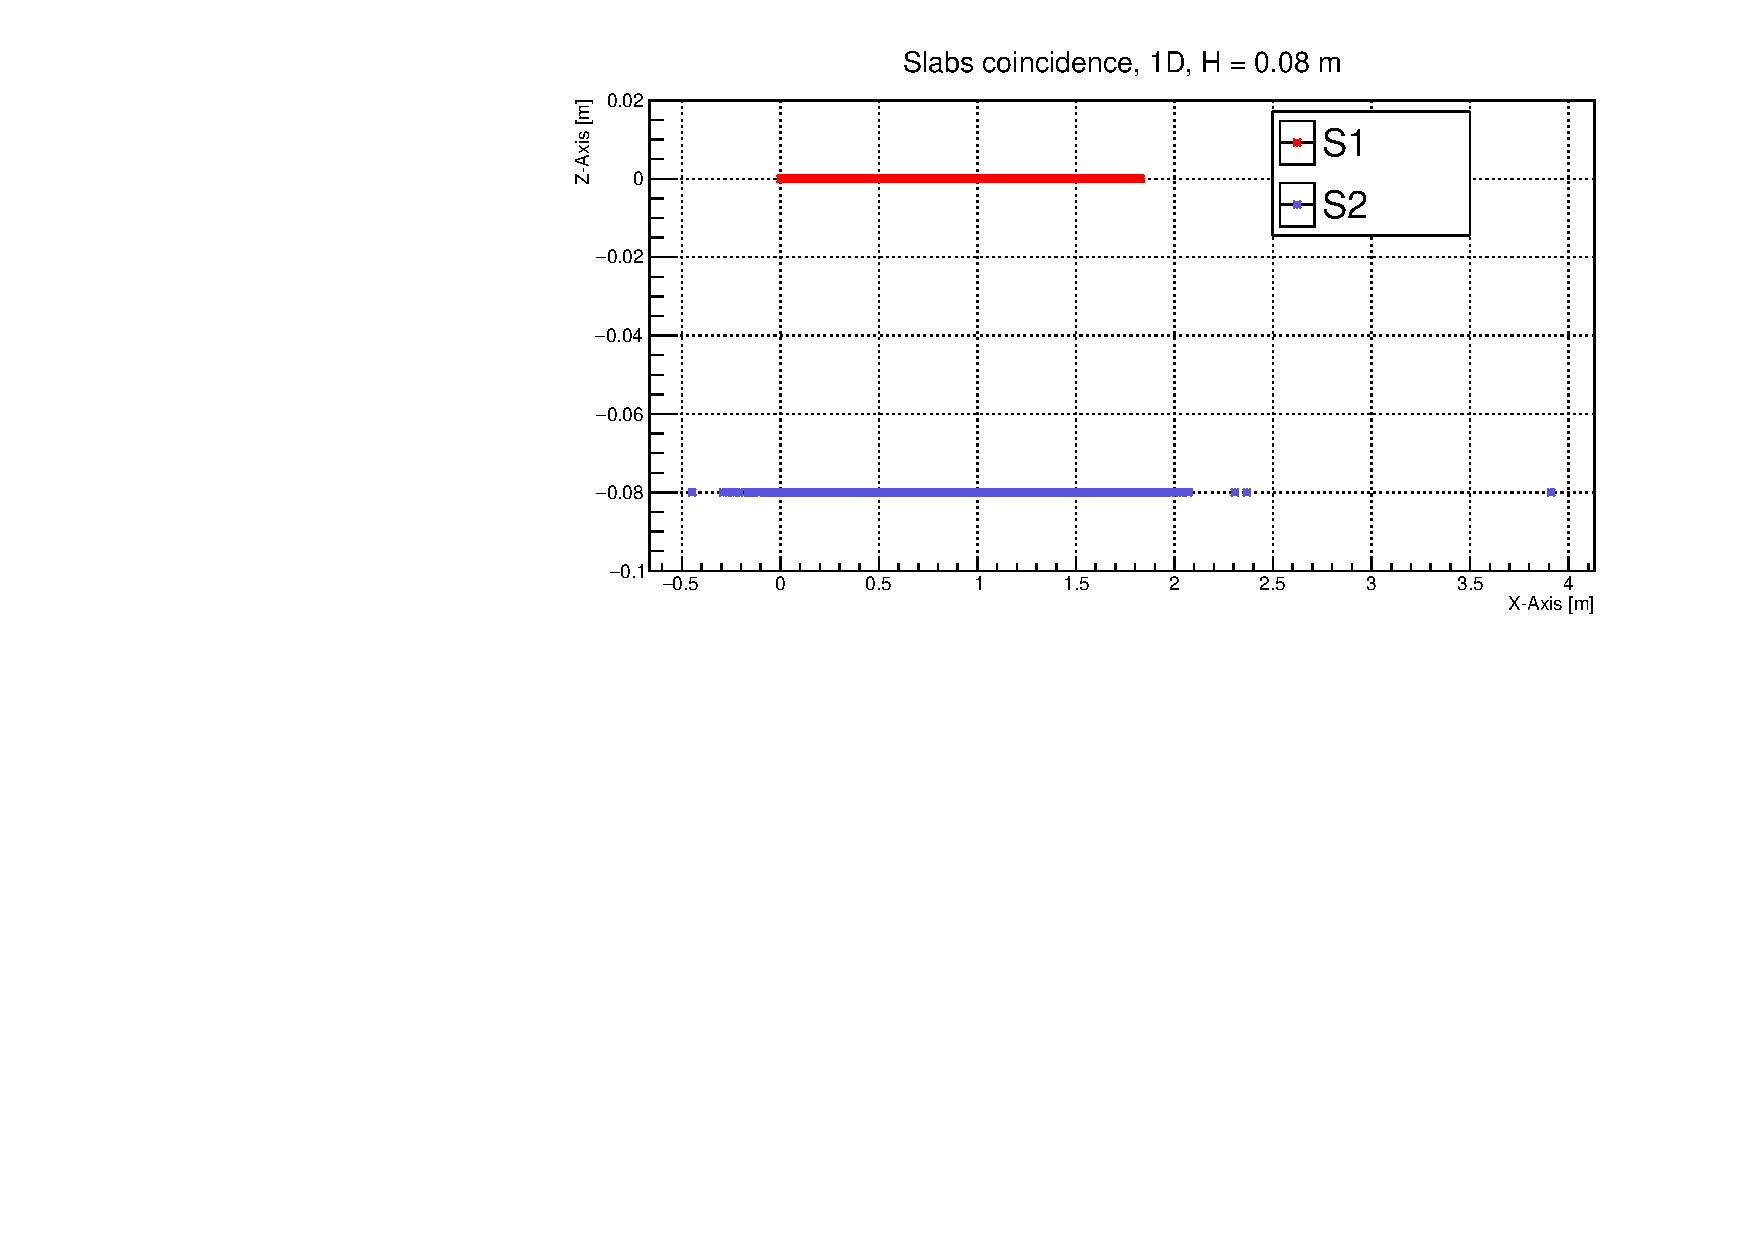
\includegraphics[scale=0.5]{img/1D.pdf}} 
	\subfloat[2D]	
	{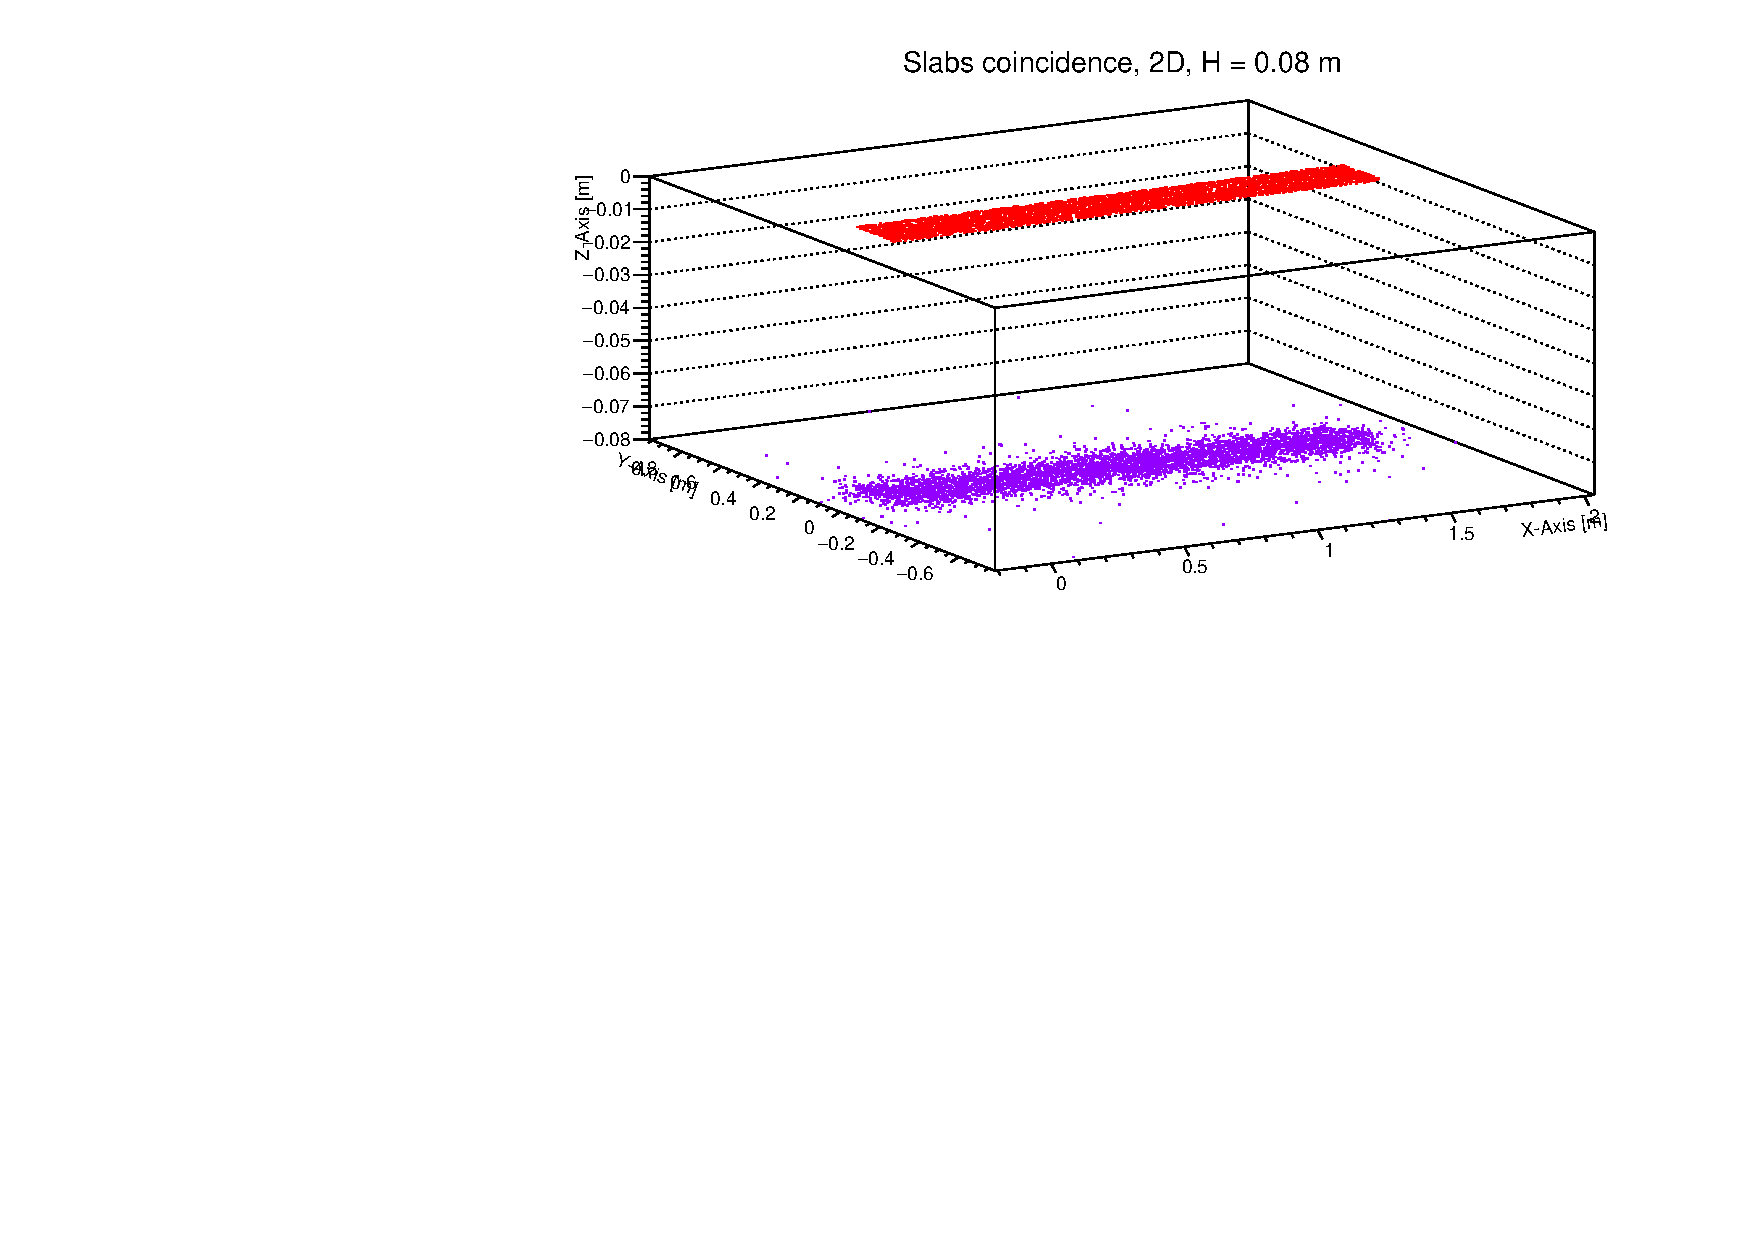
\includegraphics[scale=0.5]{img/2D.pdf}}}
	\centerline{\subfloat[3D]
		{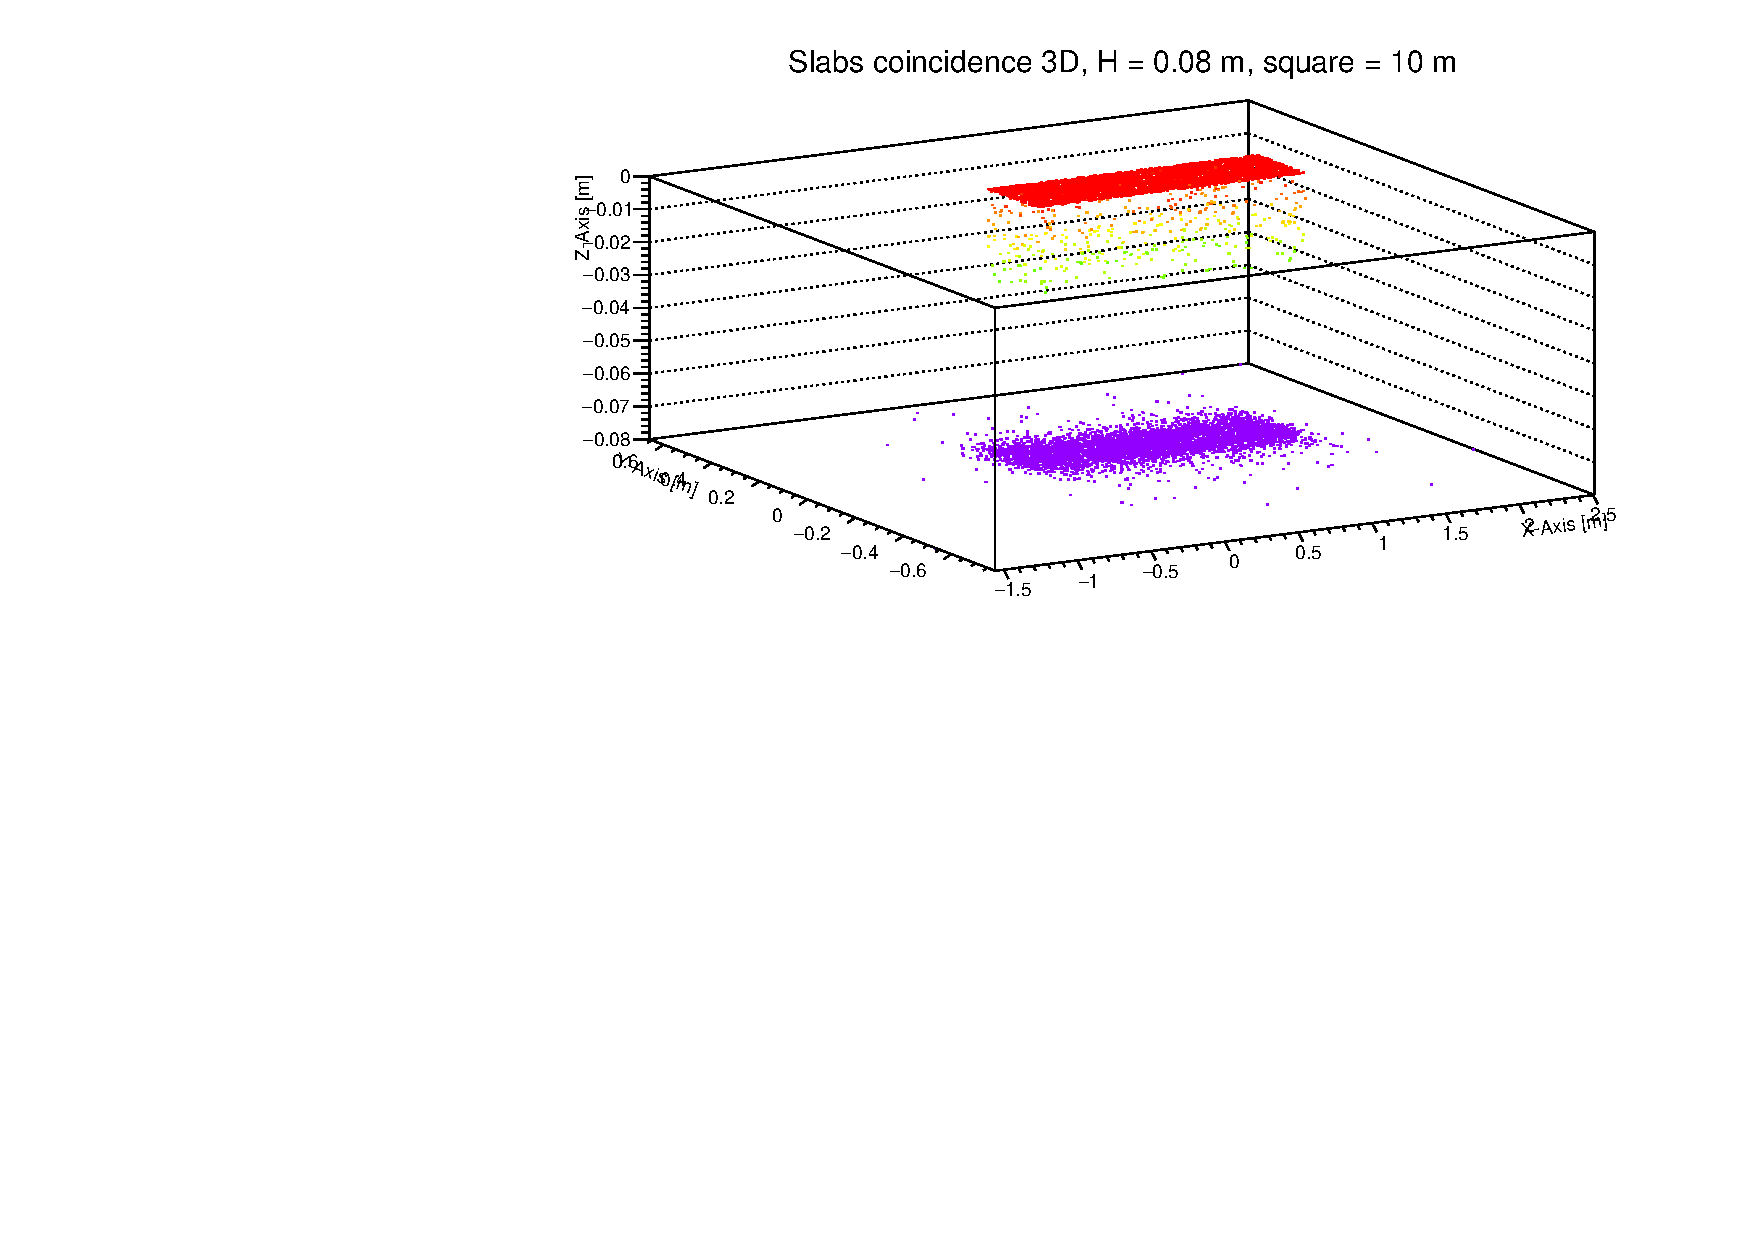
\includegraphics[scale=0.8]{img/3D.pdf}}} 
	\caption{Grafici delle simulazioni.}
	\label{nDsim_plots}
\end{figure}


\section{Grafici}
\vspace{2cm}
\begin{figure}[h]
	\centerline{\subfloat[Nr.~437]
		{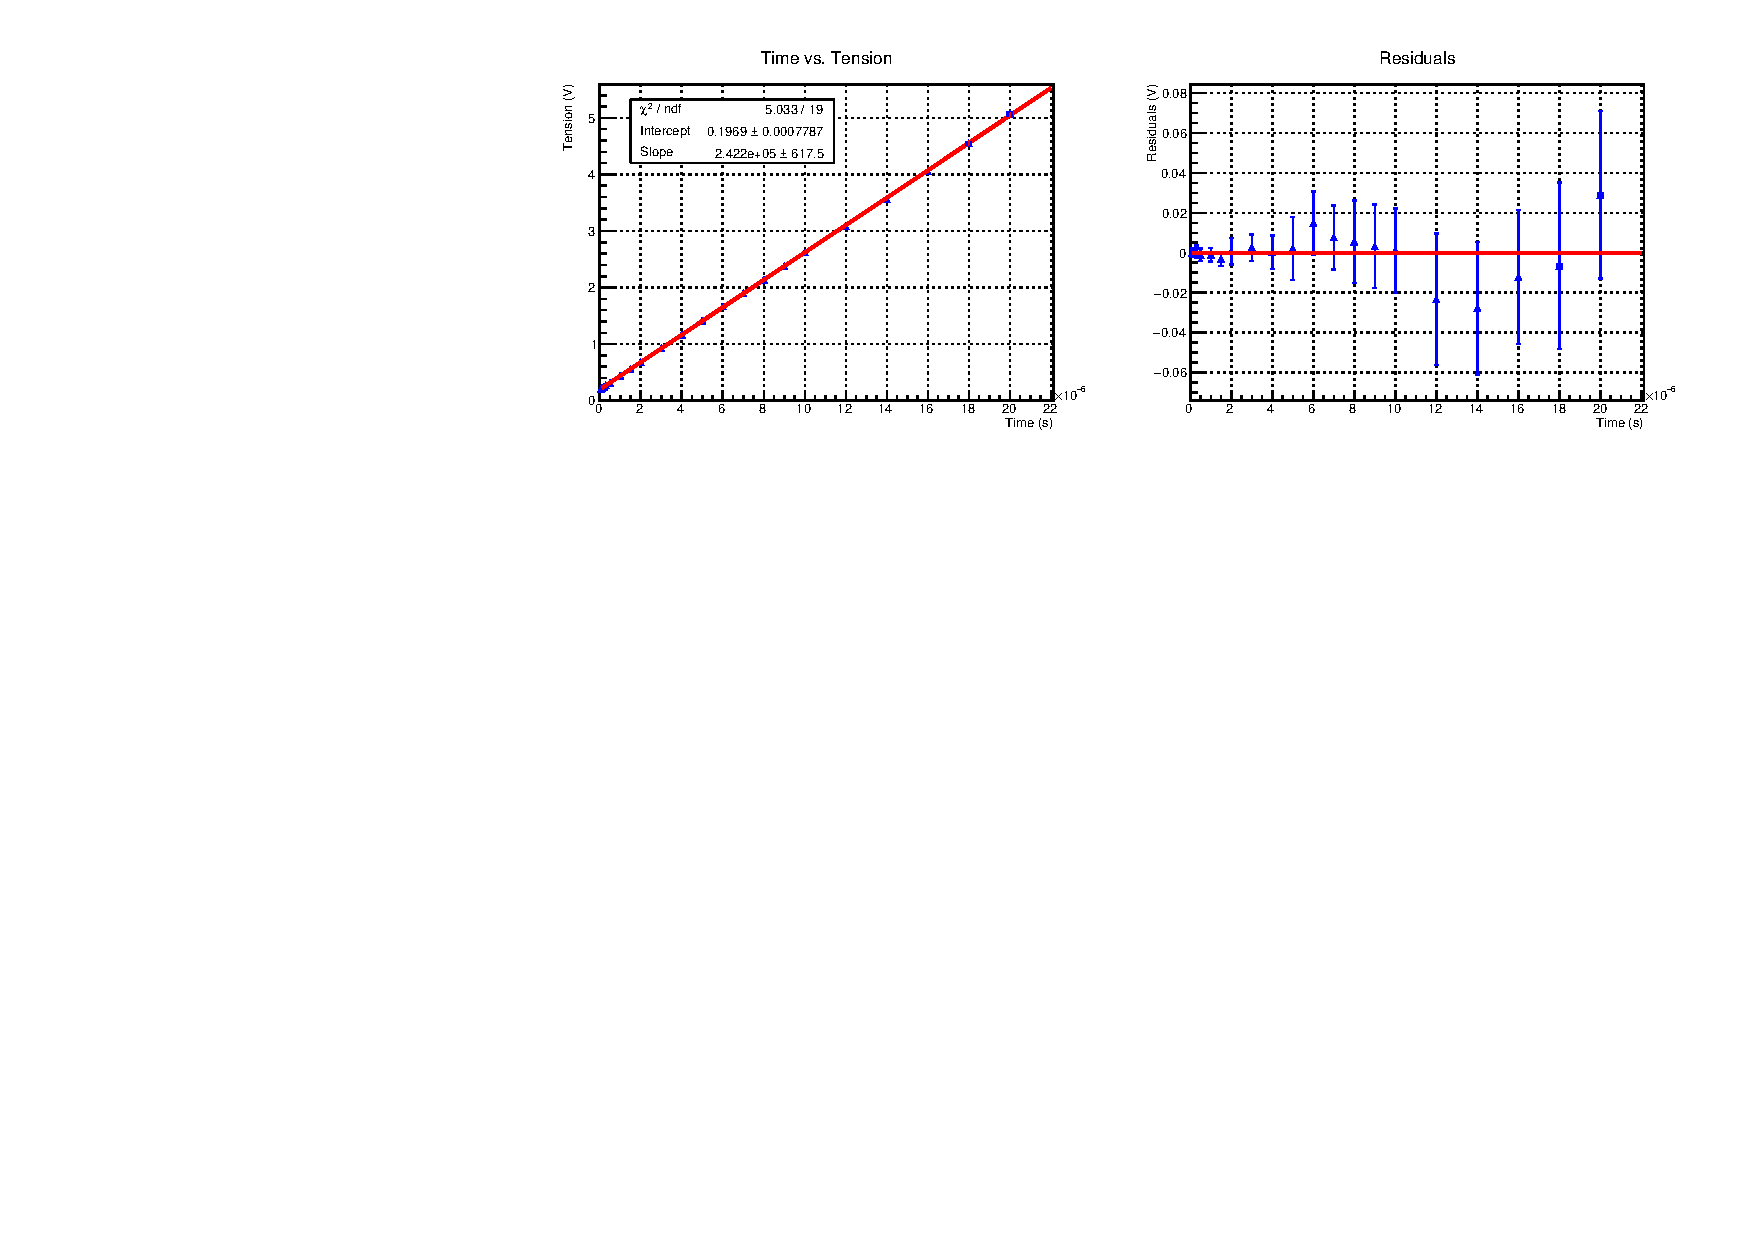
\includegraphics[scale=1.0]{img/time_tens_437.pdf}}}
	\centerline{\subfloat[Nr.~467]
		{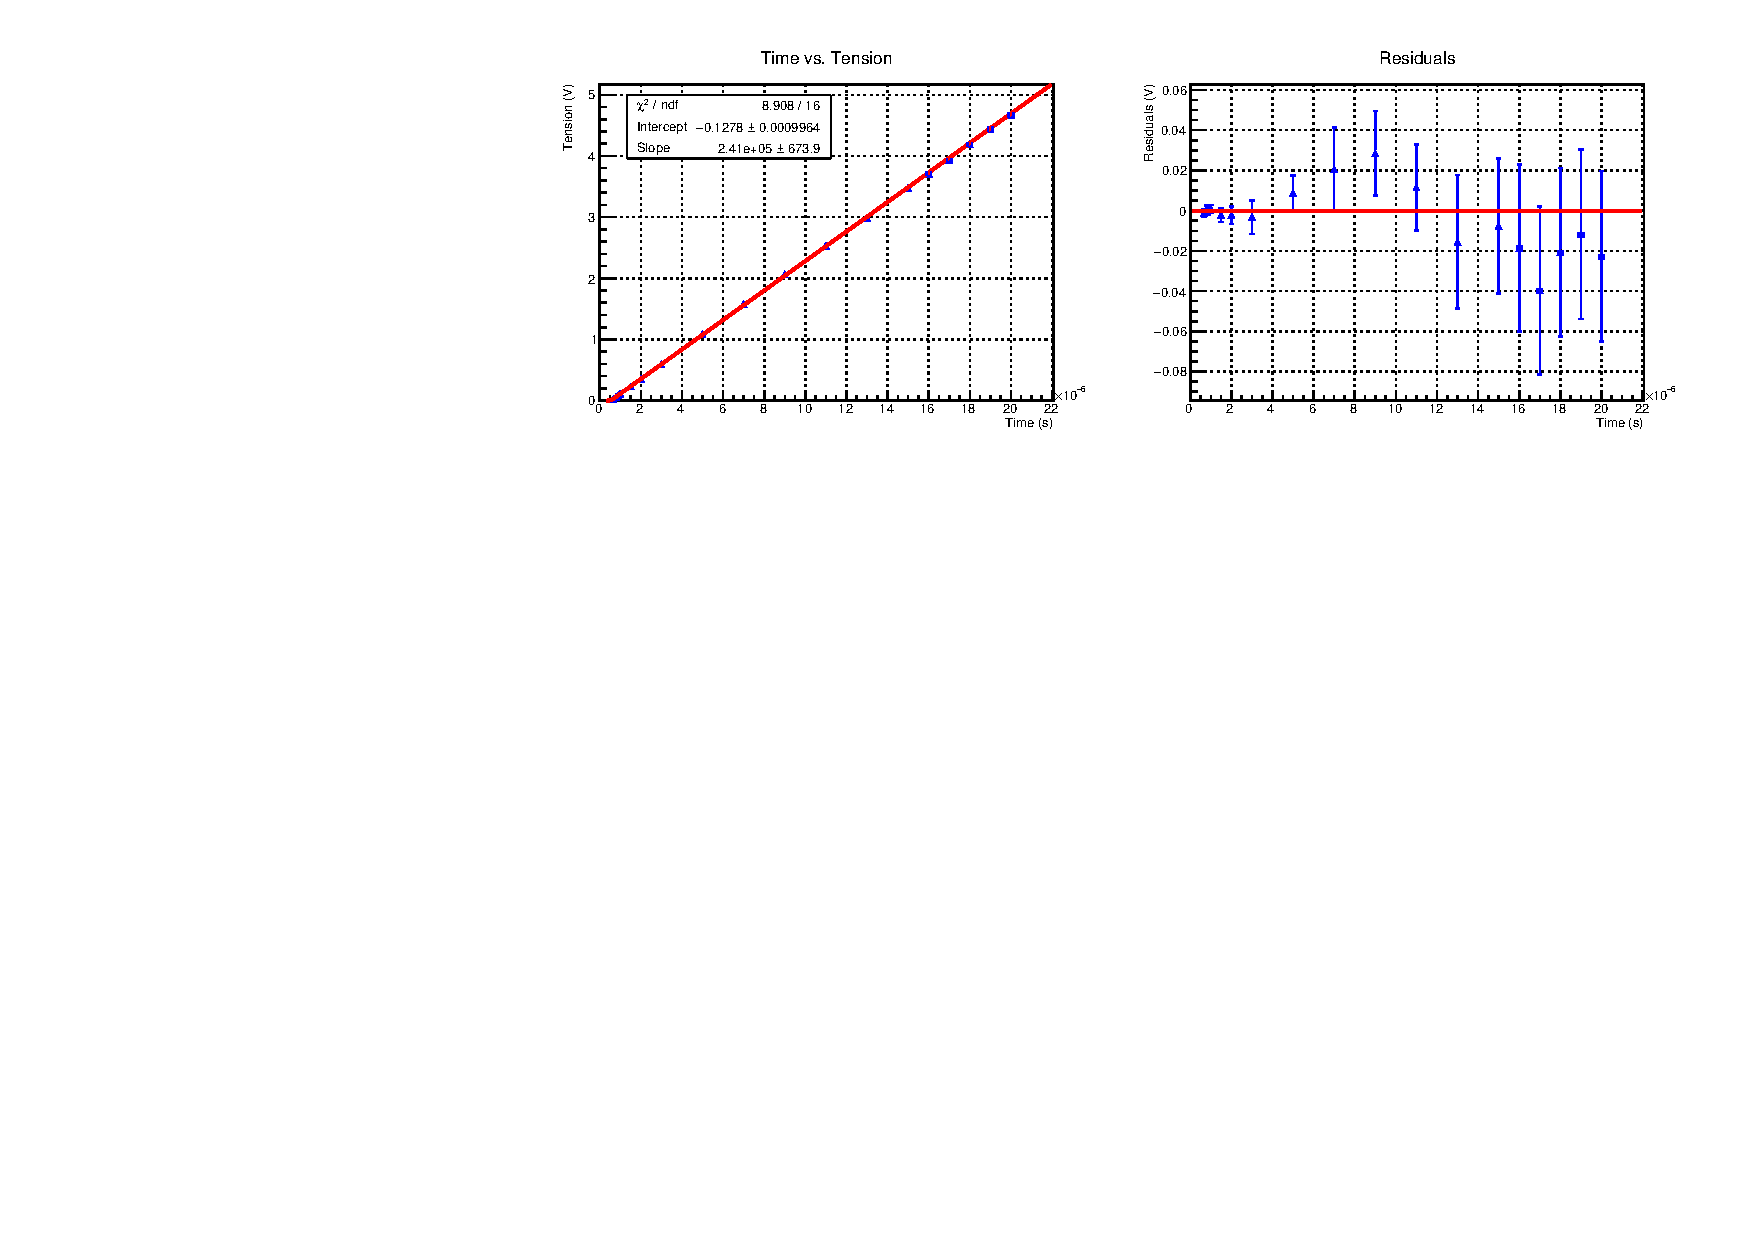
\includegraphics[scale=1.0]{img/time_tens_467.pdf}}} 
	\caption{Valori di tensione erogati in base al ritardo.}
	\label{time_tens}
\end{figure}
\begin{figure}[h]
	\centerline{\subfloat[Nr.~437]
		{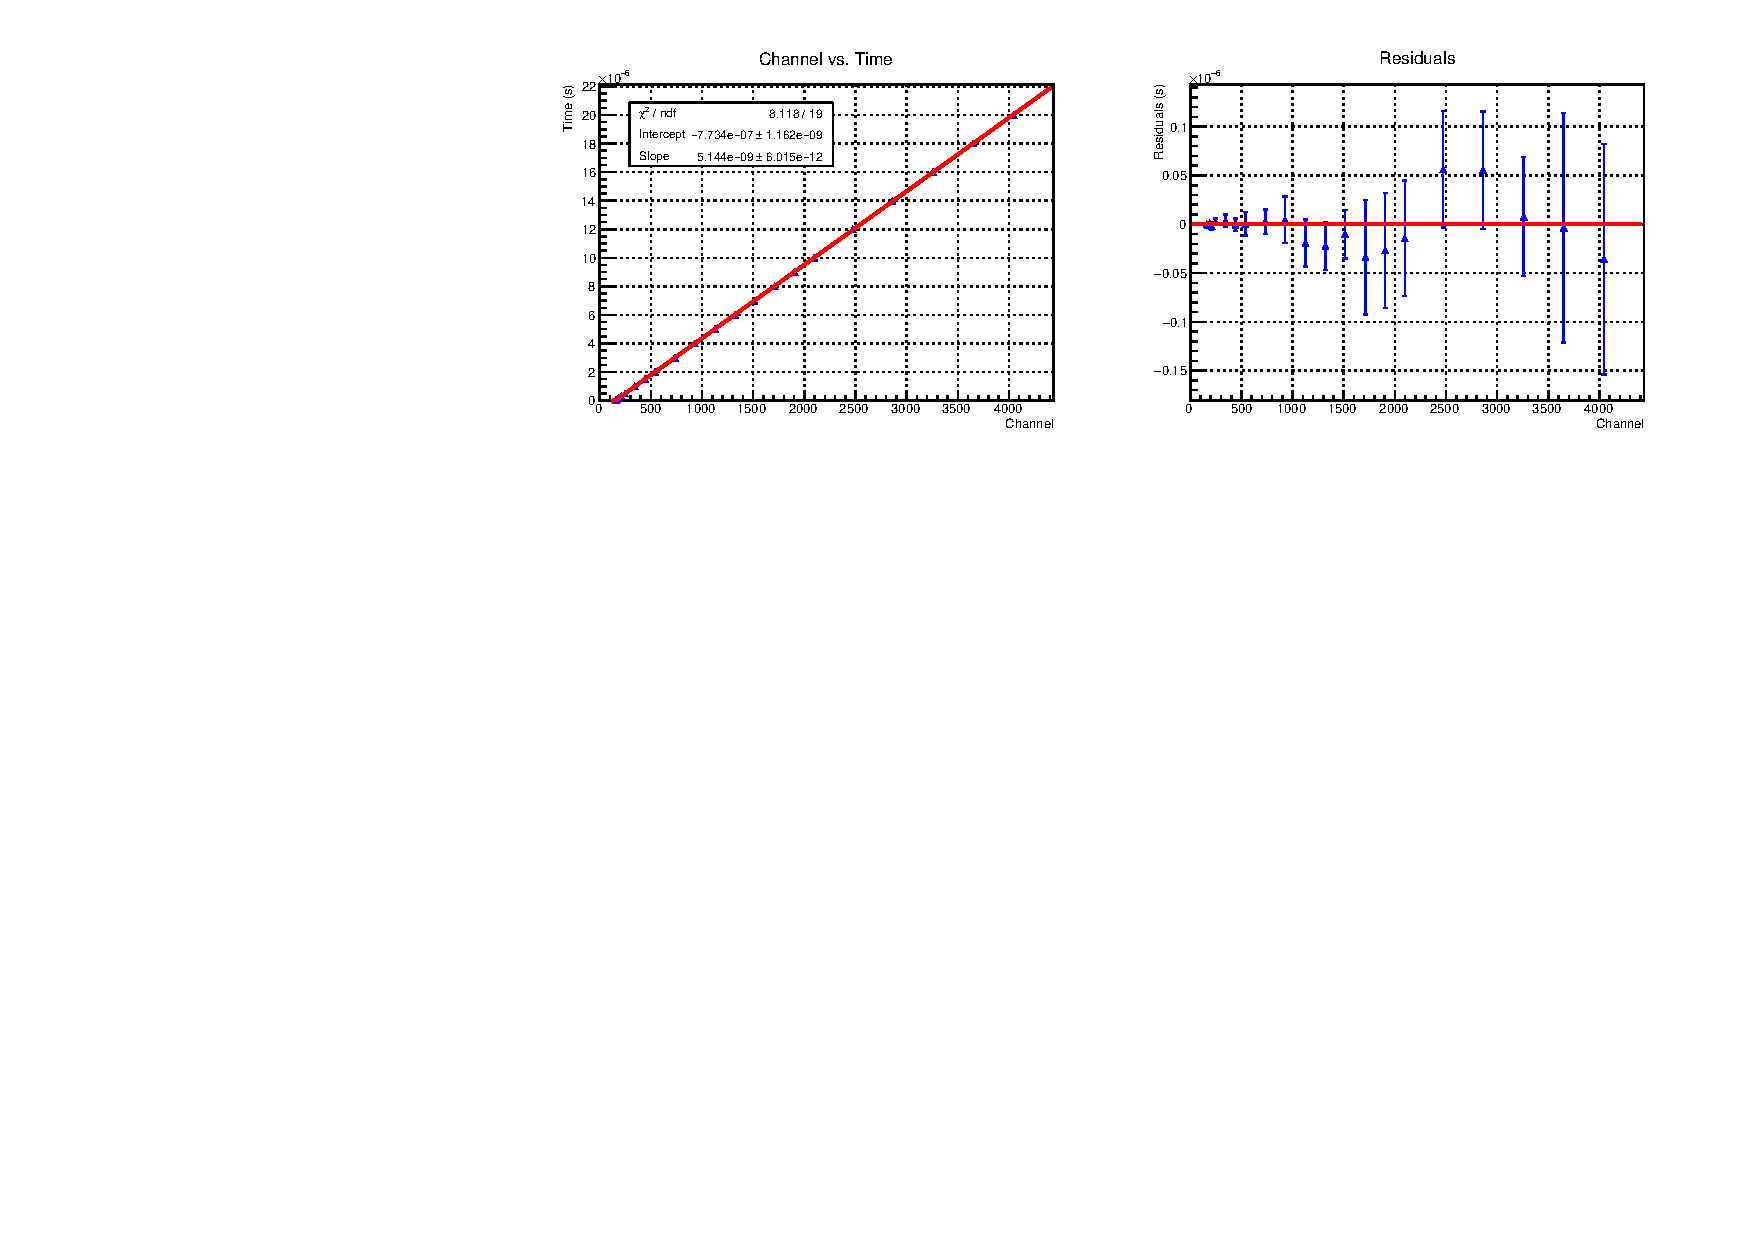
\includegraphics[scale=1.0]{img/chan_time_437.pdf}}}
	\centerline{\subfloat[Nr.~467]
		{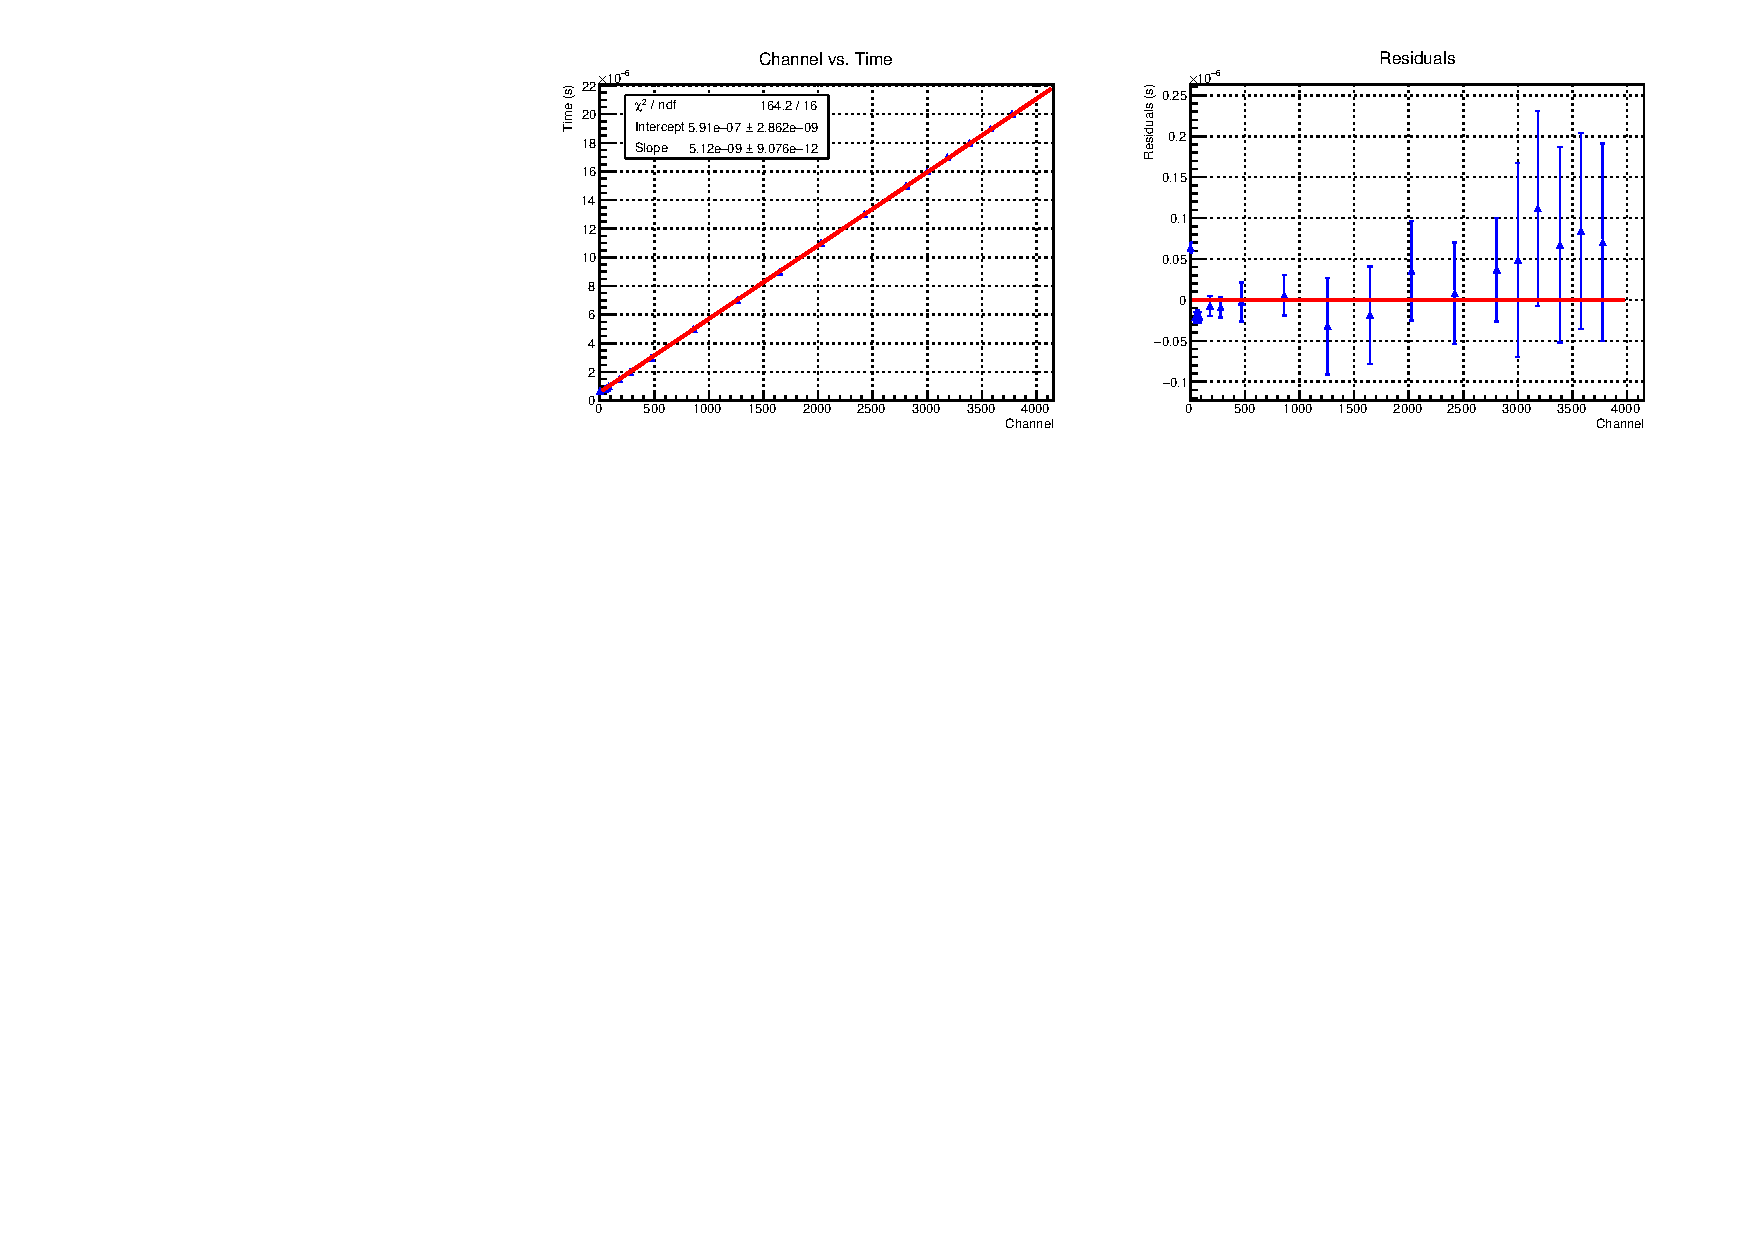
\includegraphics[scale=1.0]{img/chan_time_467.pdf}}}
	\caption{Canali corrispondenti ai ritardi impostati.}
	\label{chan_time}
\end{figure}
\begin{figure}[h]
	\centerline{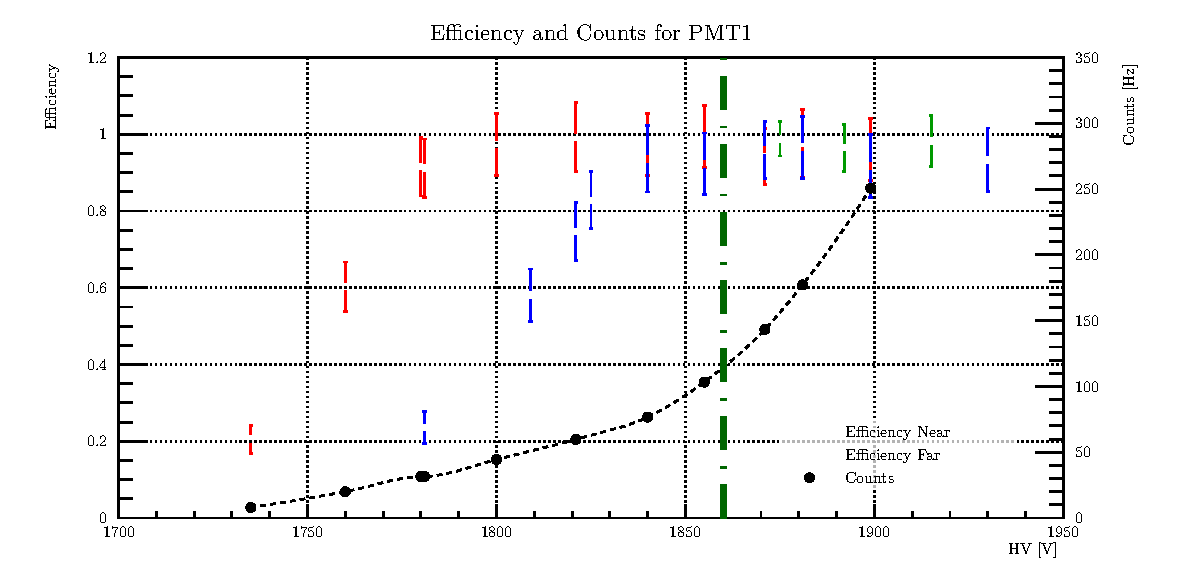
\includegraphics[scale=0.8]{img/eff1.pdf}}
\end{figure}
\begin{figure}[h]
	\centerline{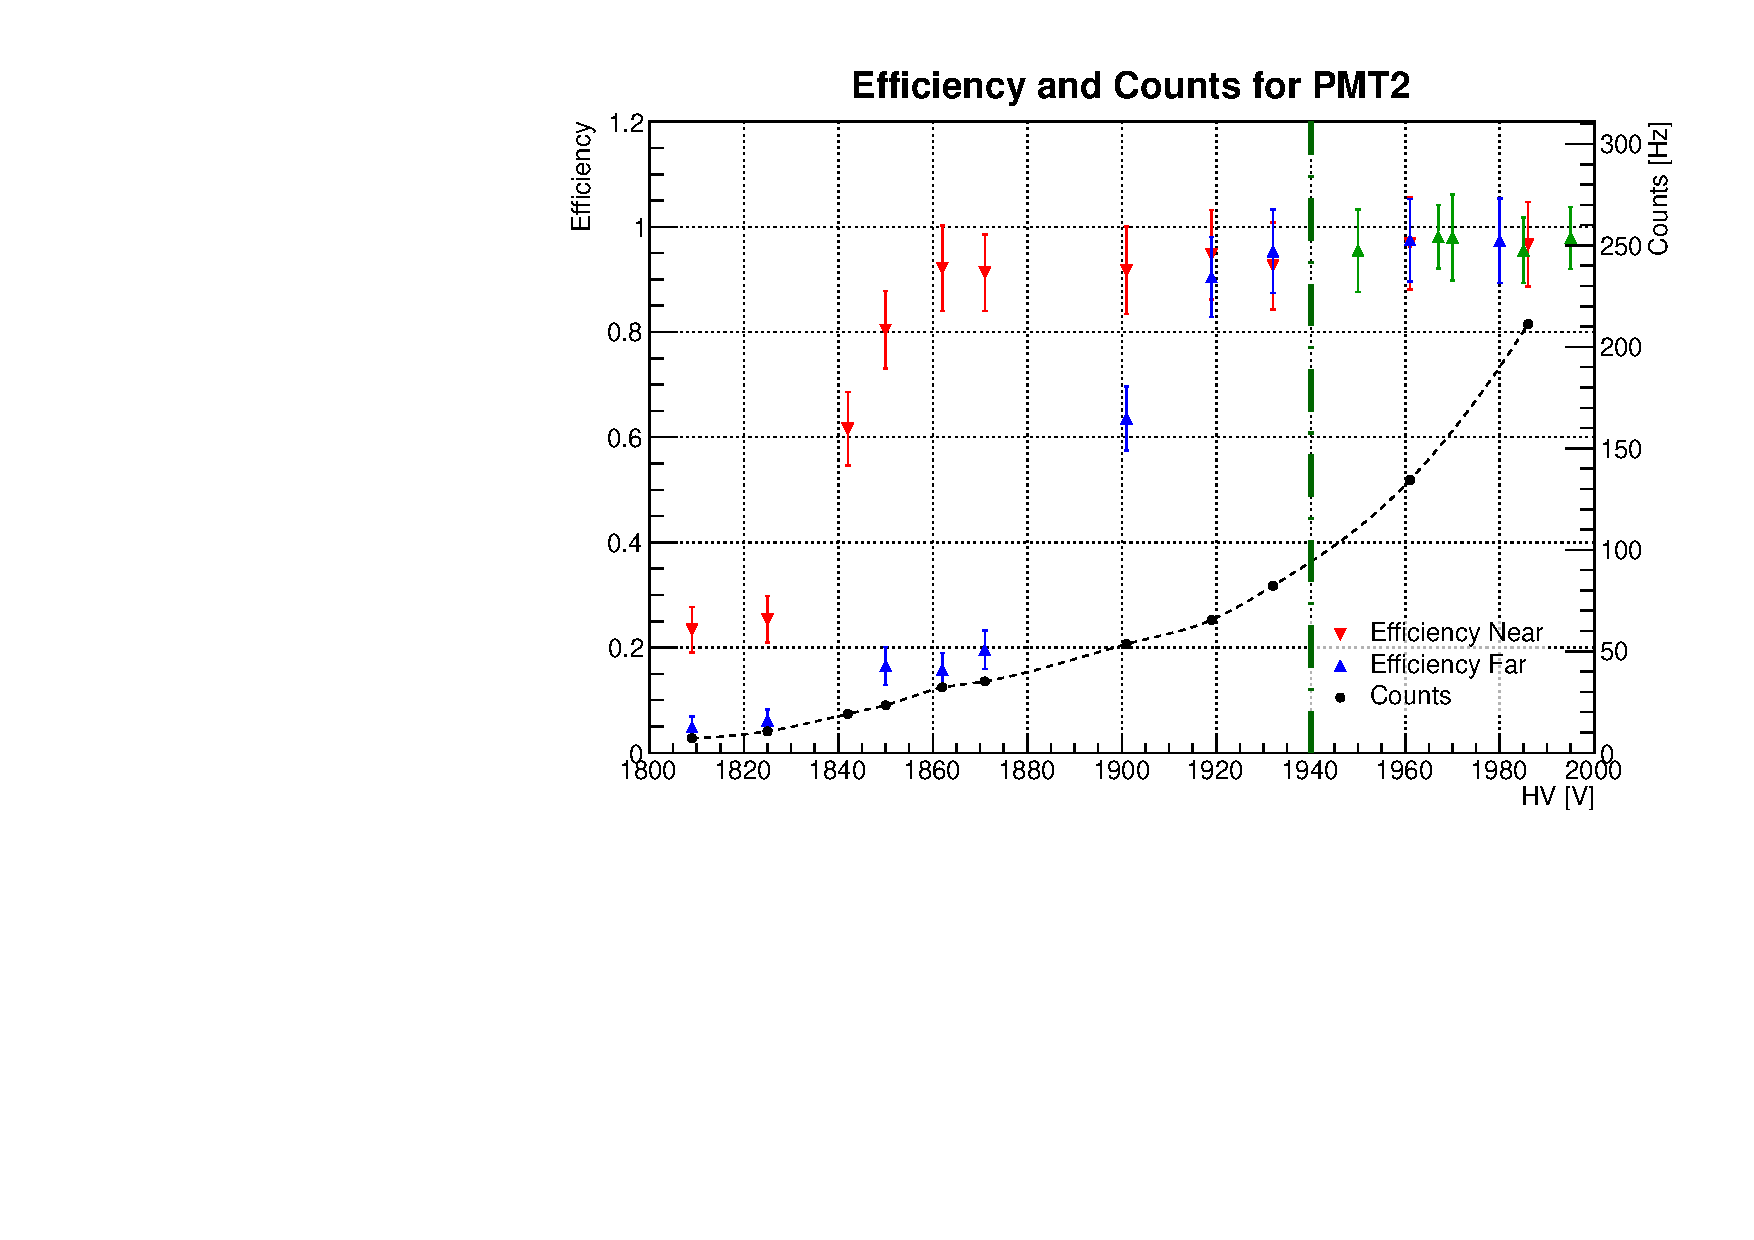
\includegraphics[scale=0.8]{img/eff2.pdf}}	
\end{figure}
\begin{figure}[h]
	\centerline{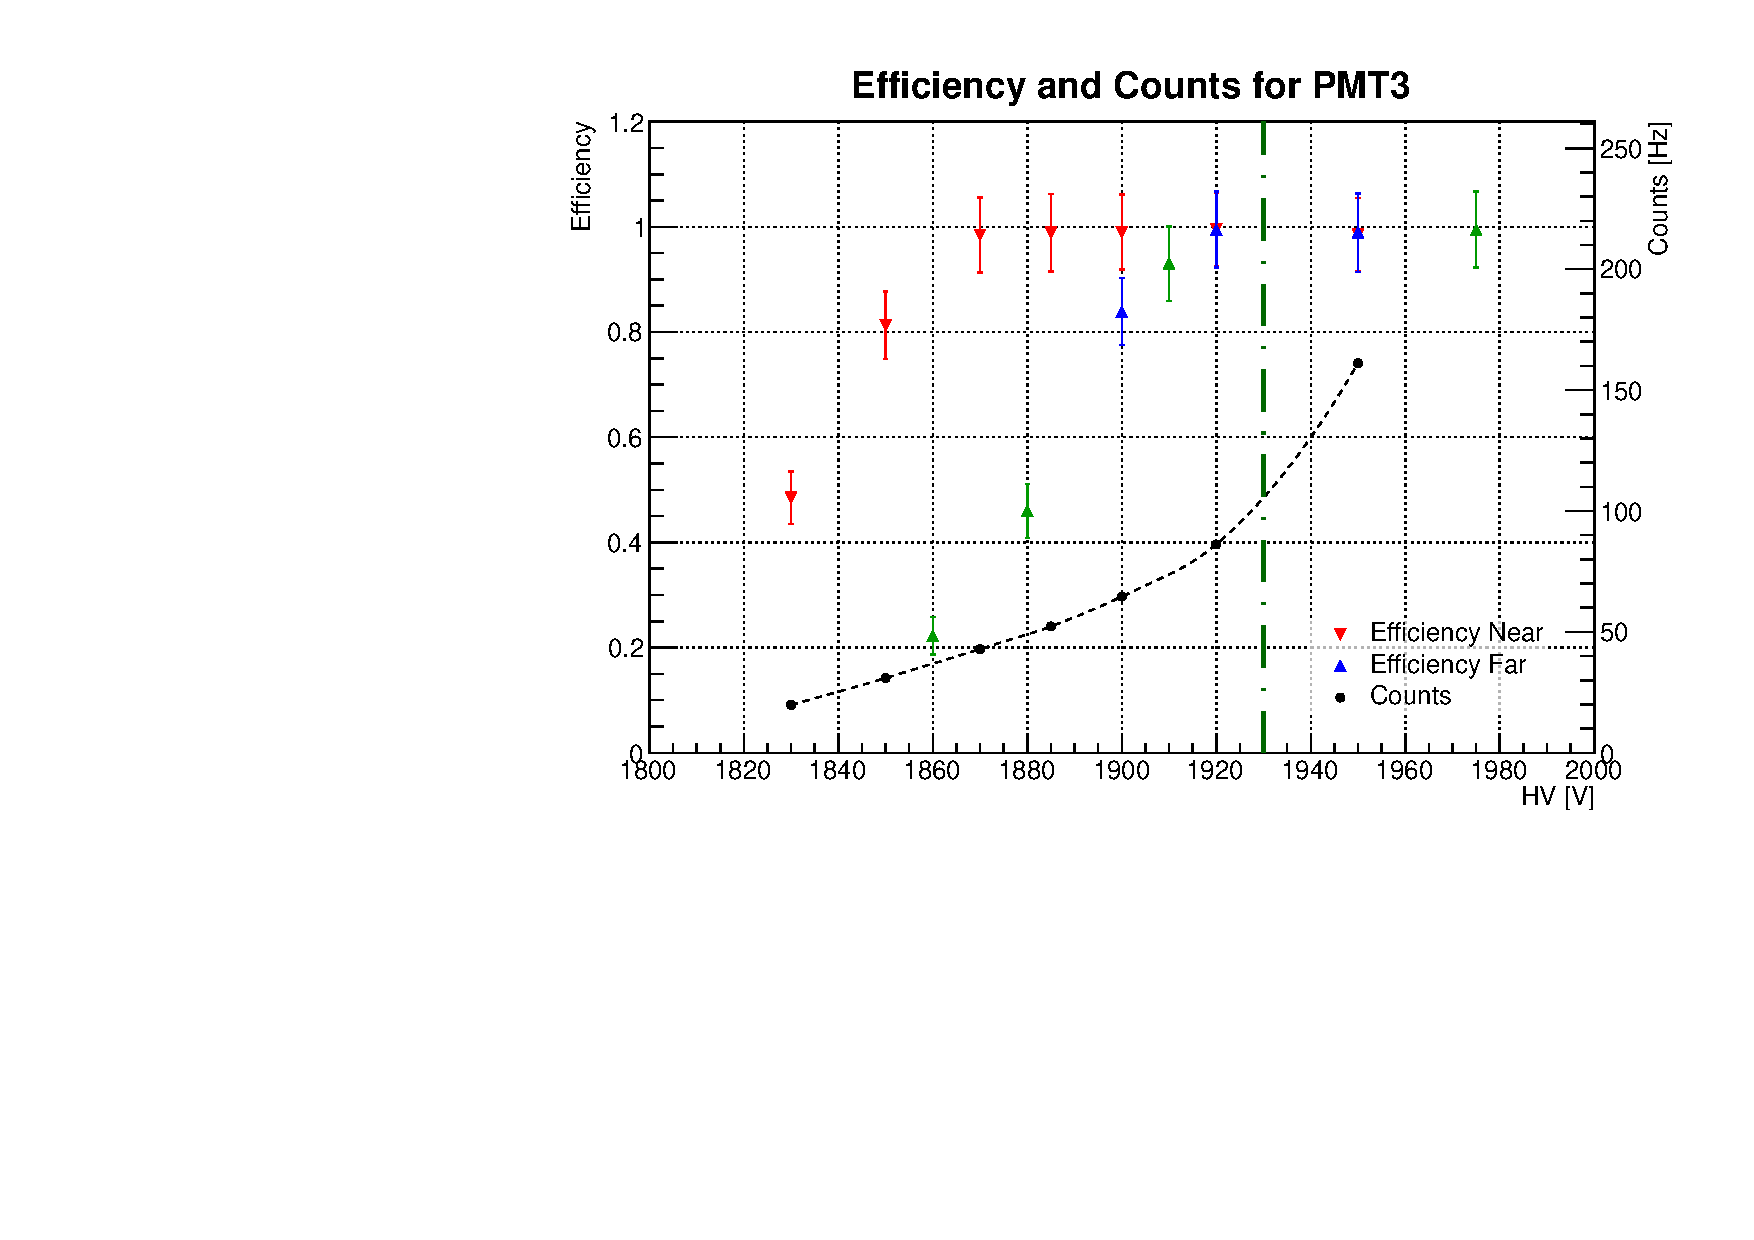
\includegraphics[scale=0.8]{img/eff3.pdf}}	
\end{figure}
\begin{figure}[h]
	\centerline{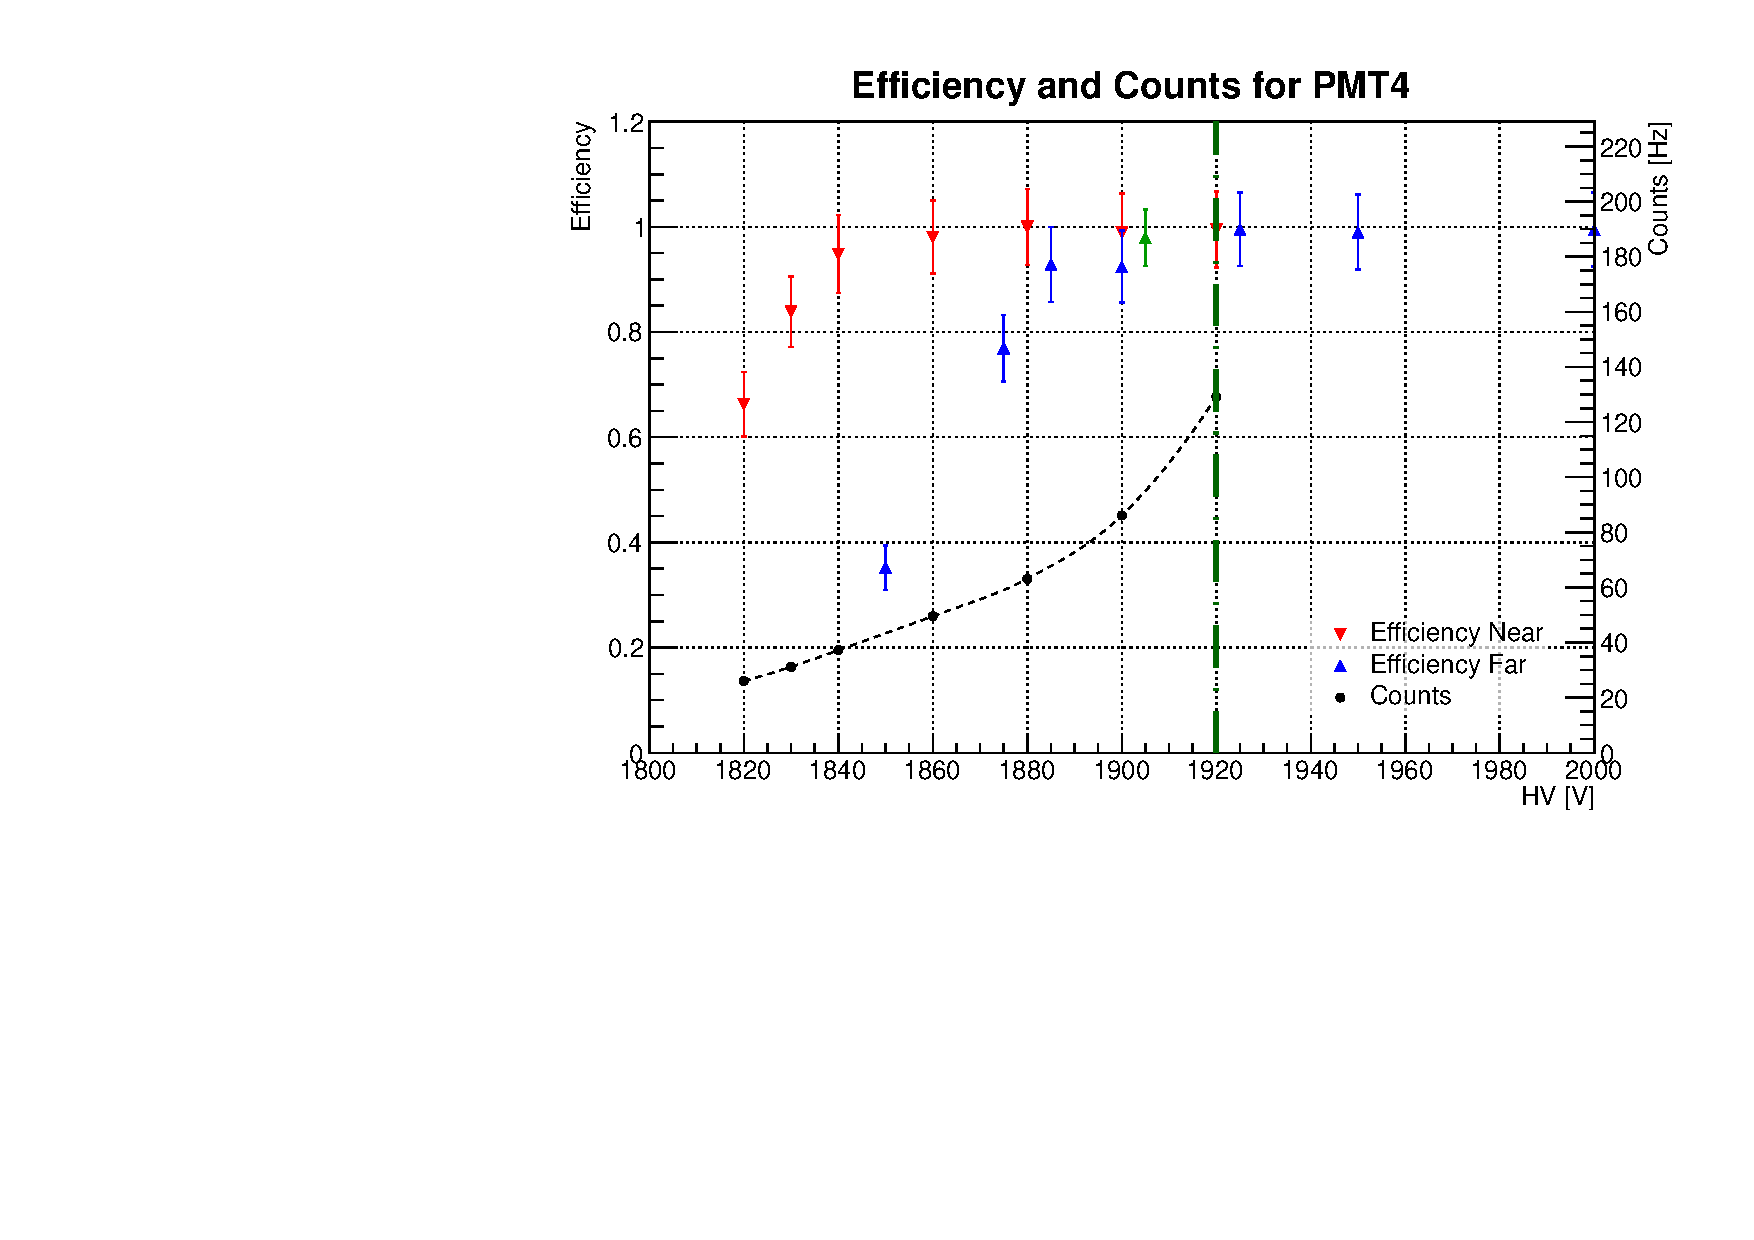
\includegraphics[scale=0.8]{img/eff4.pdf}}
\end{figure}
\begin{figure}[h]
	\centerline{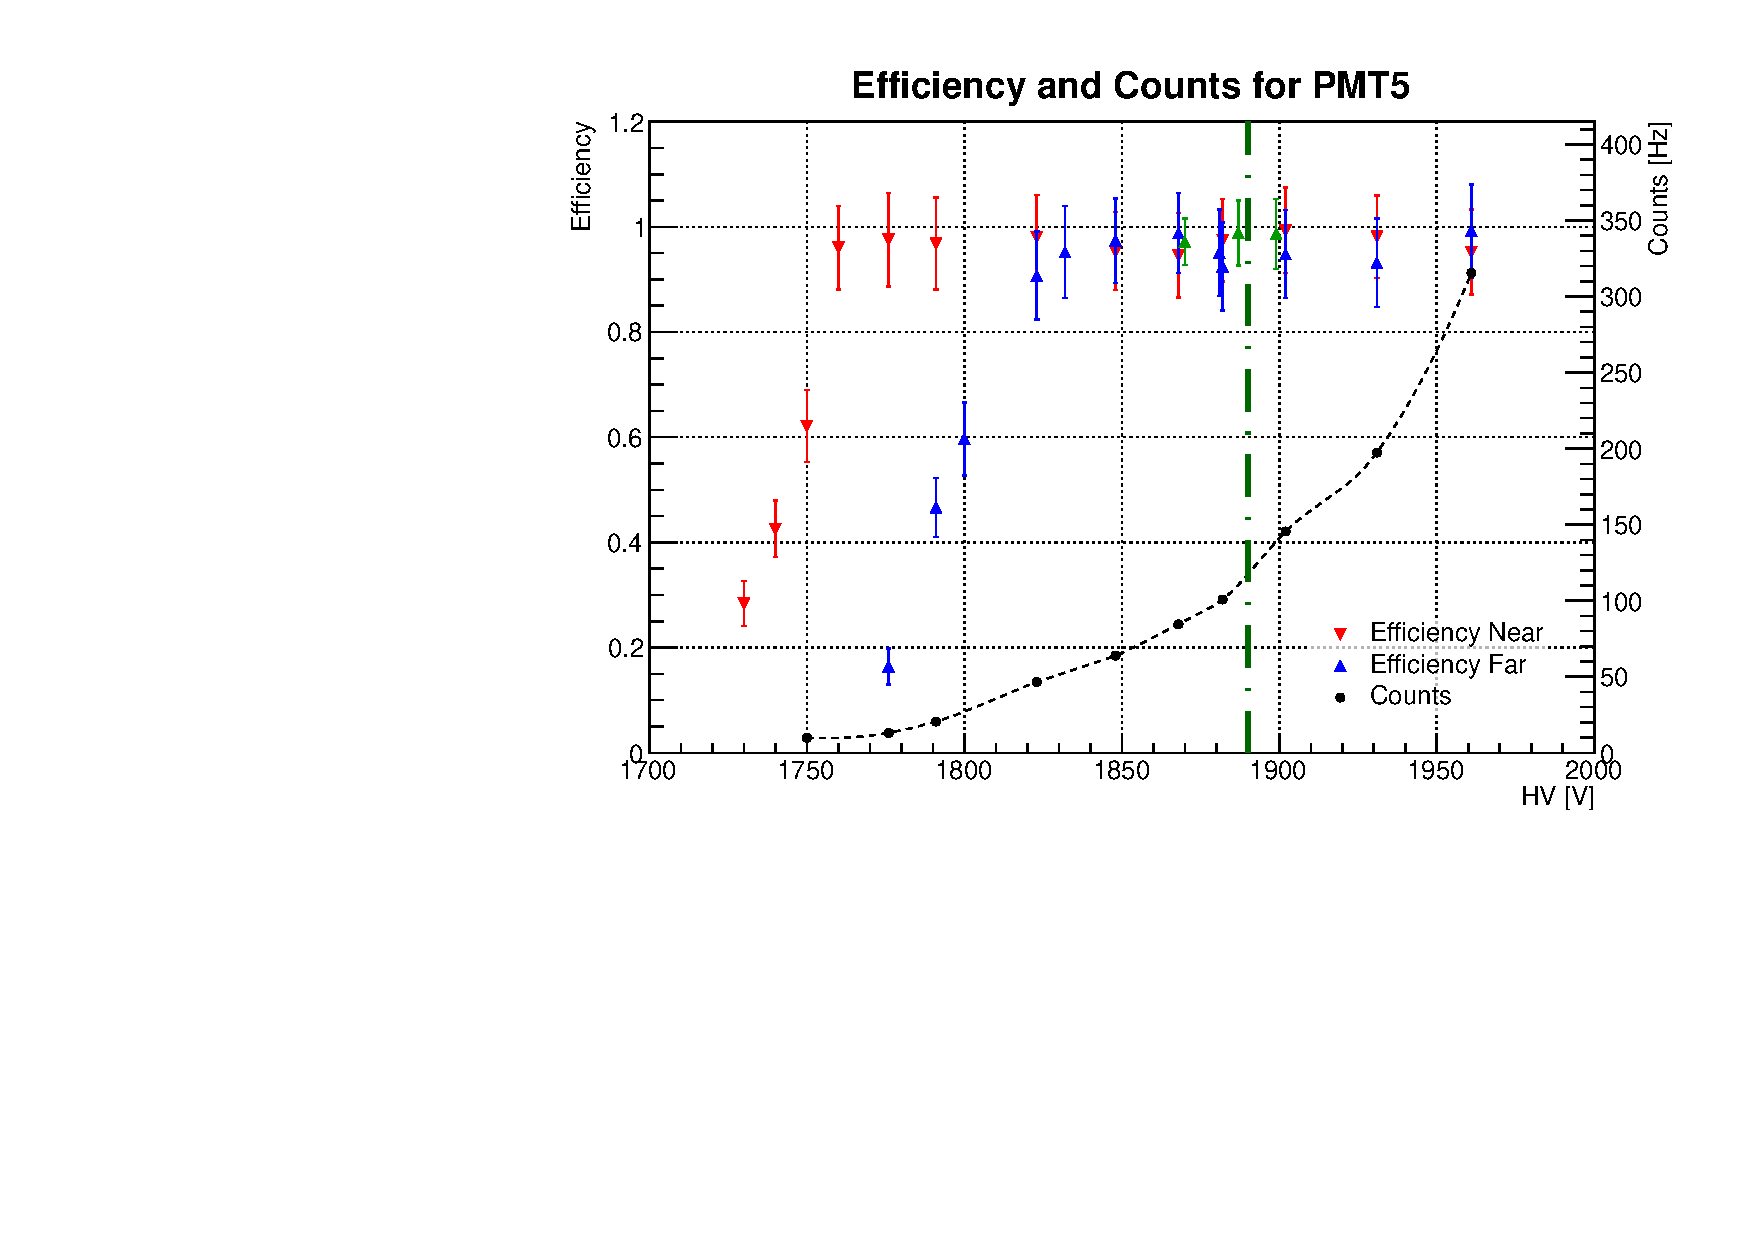
\includegraphics[scale=0.8]{img/eff5.pdf}}
\end{figure}
\begin{figure}[h]
	\centerline{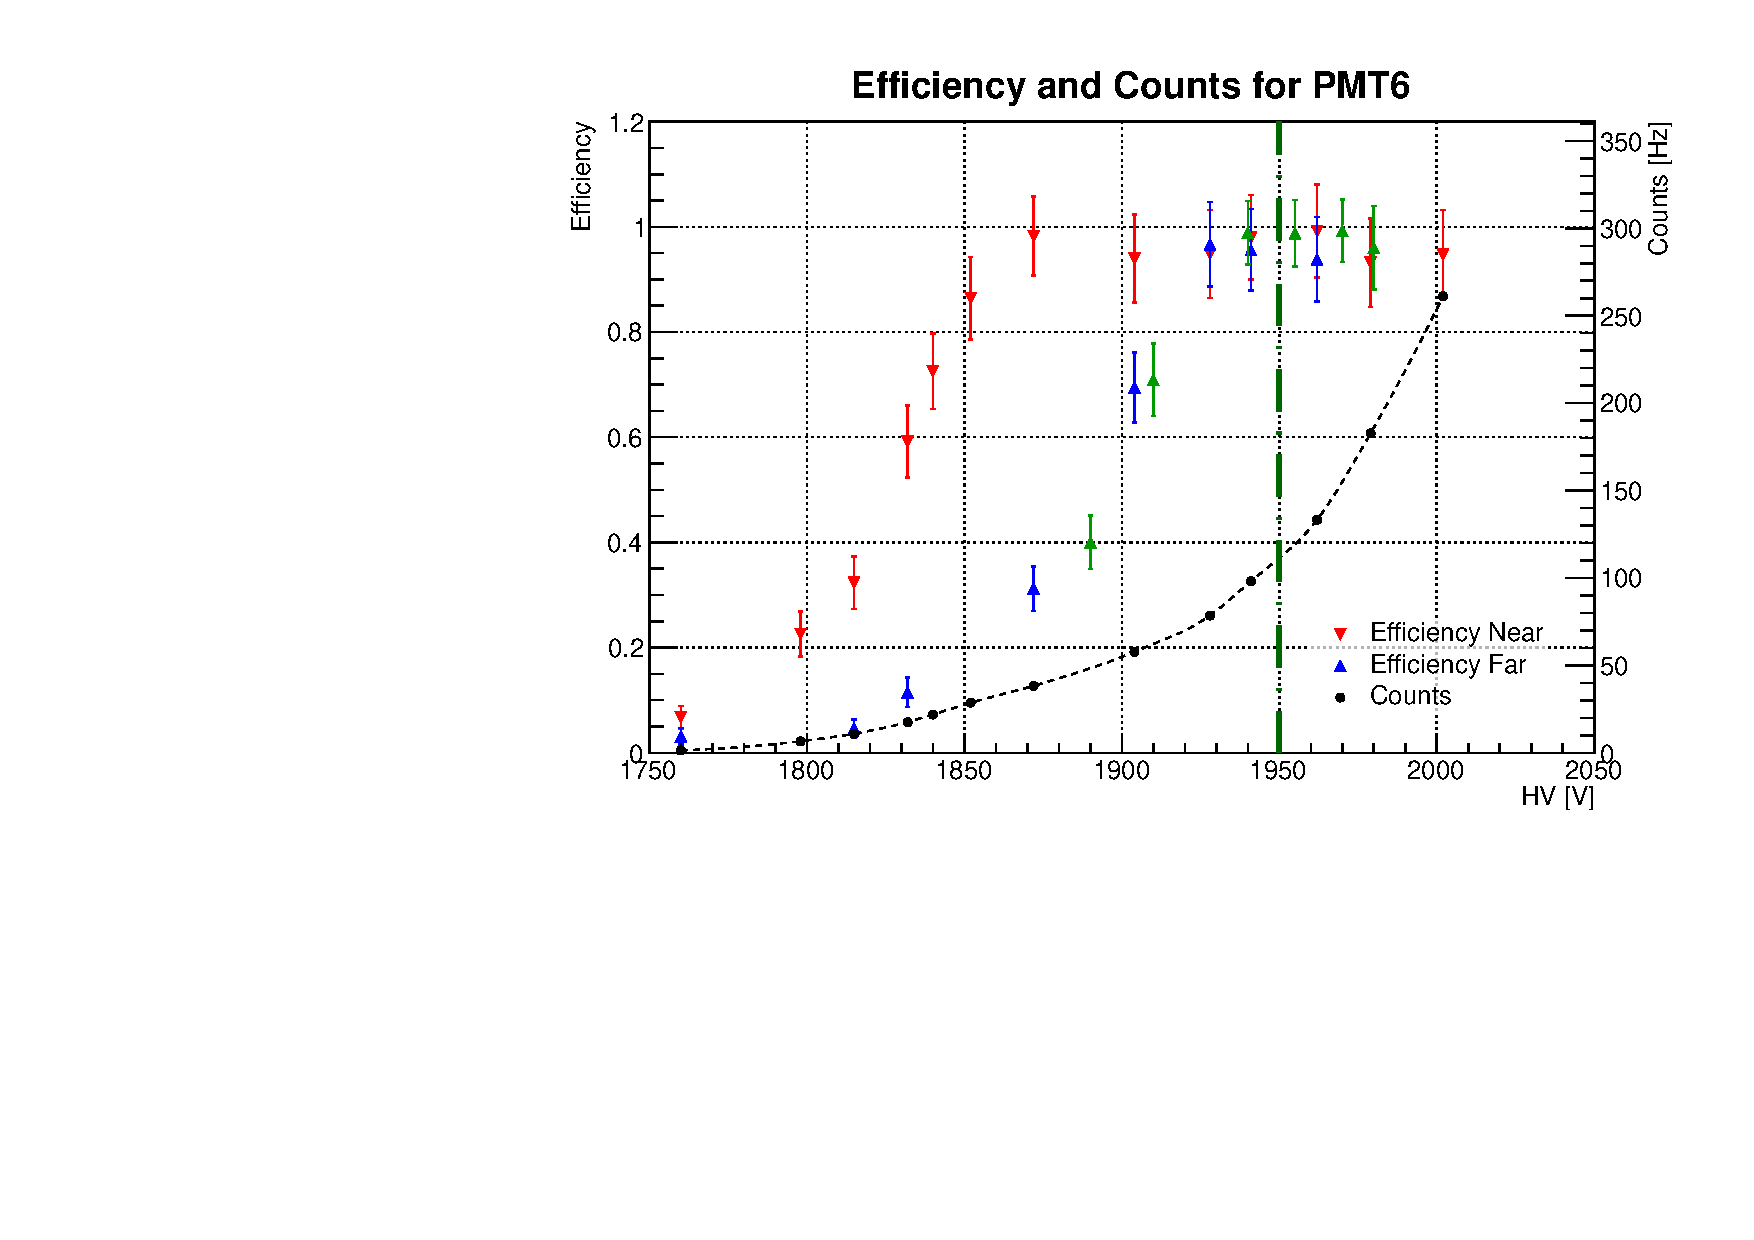
\includegraphics[scale=0.8]{img/eff6.pdf}}
\end{figure}
\begin{figure}[h]
	\centerline{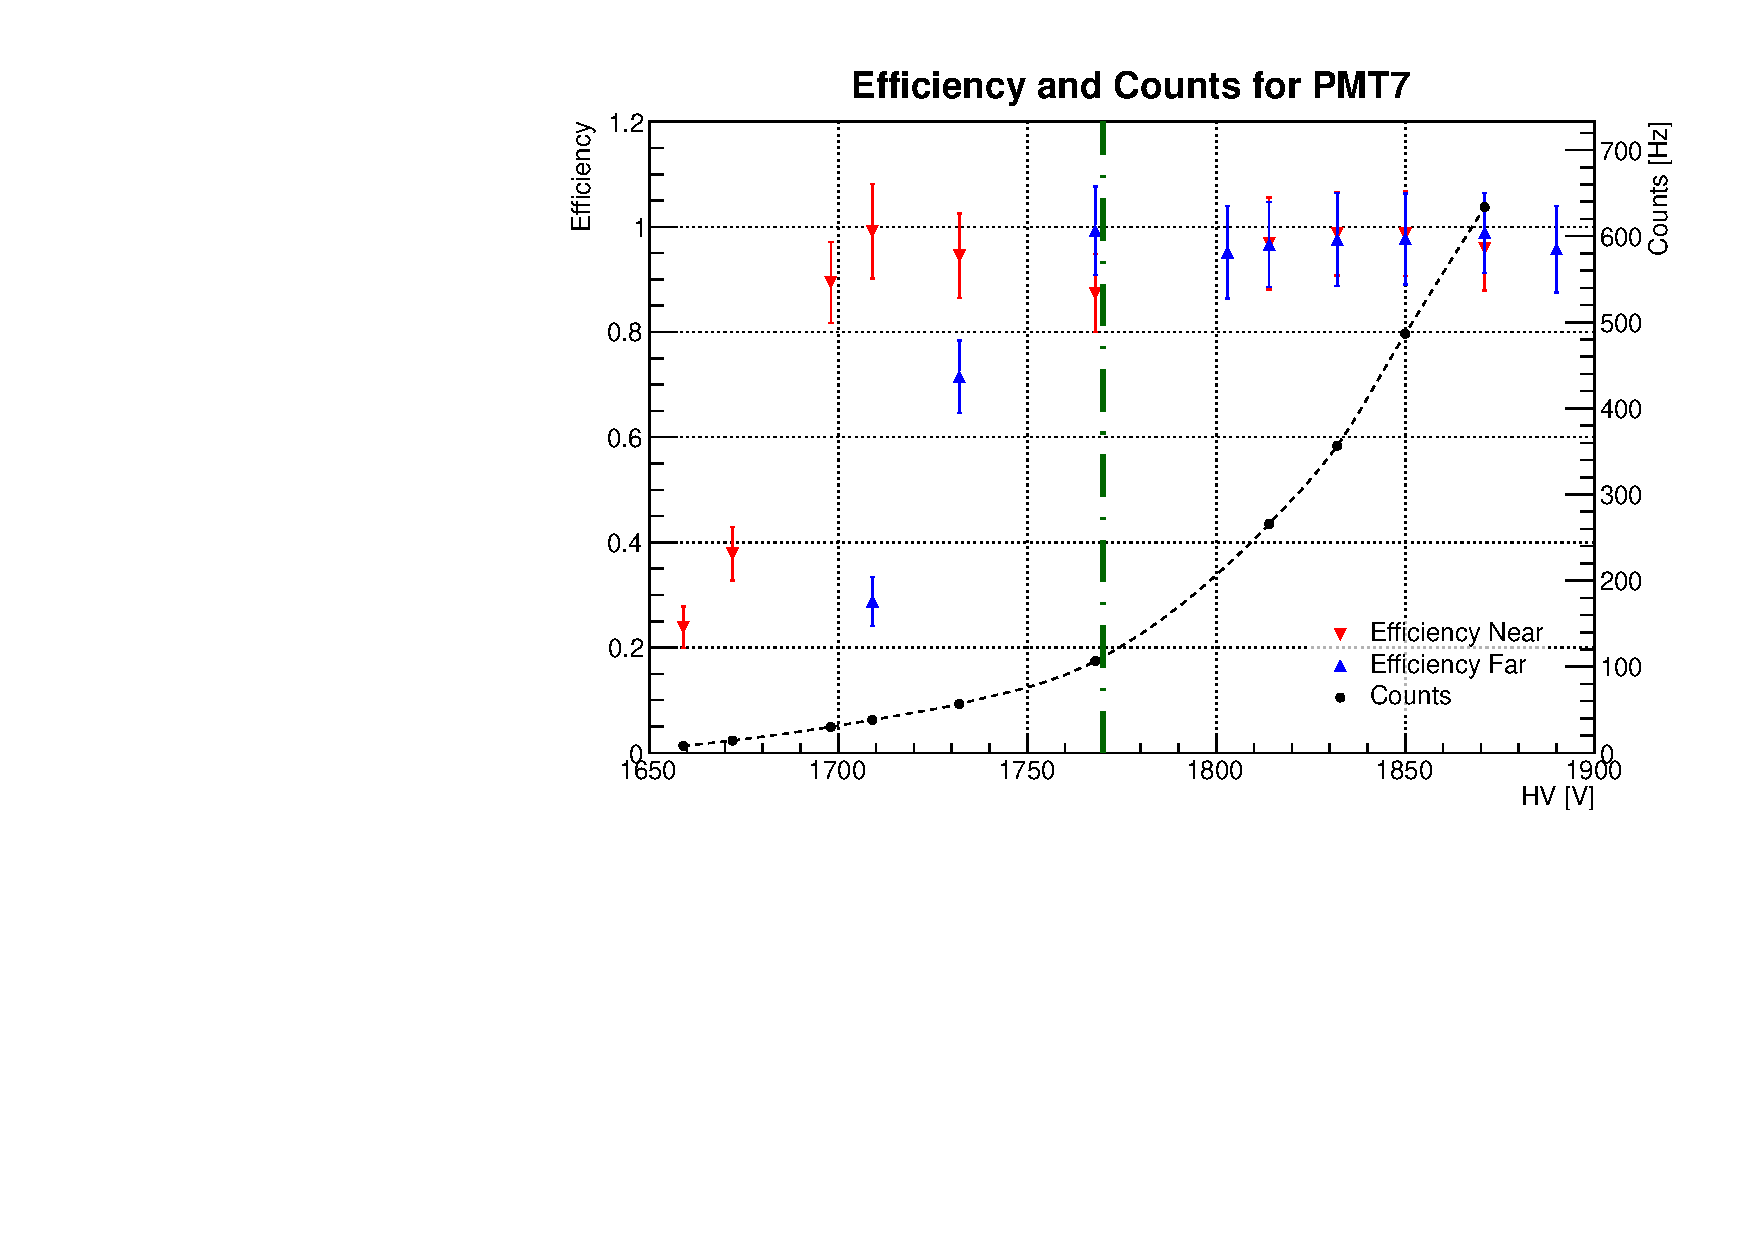
\includegraphics[scale=0.8]{img/eff7.pdf}}
\end{figure}
\begin{figure}[h]
	\centerline{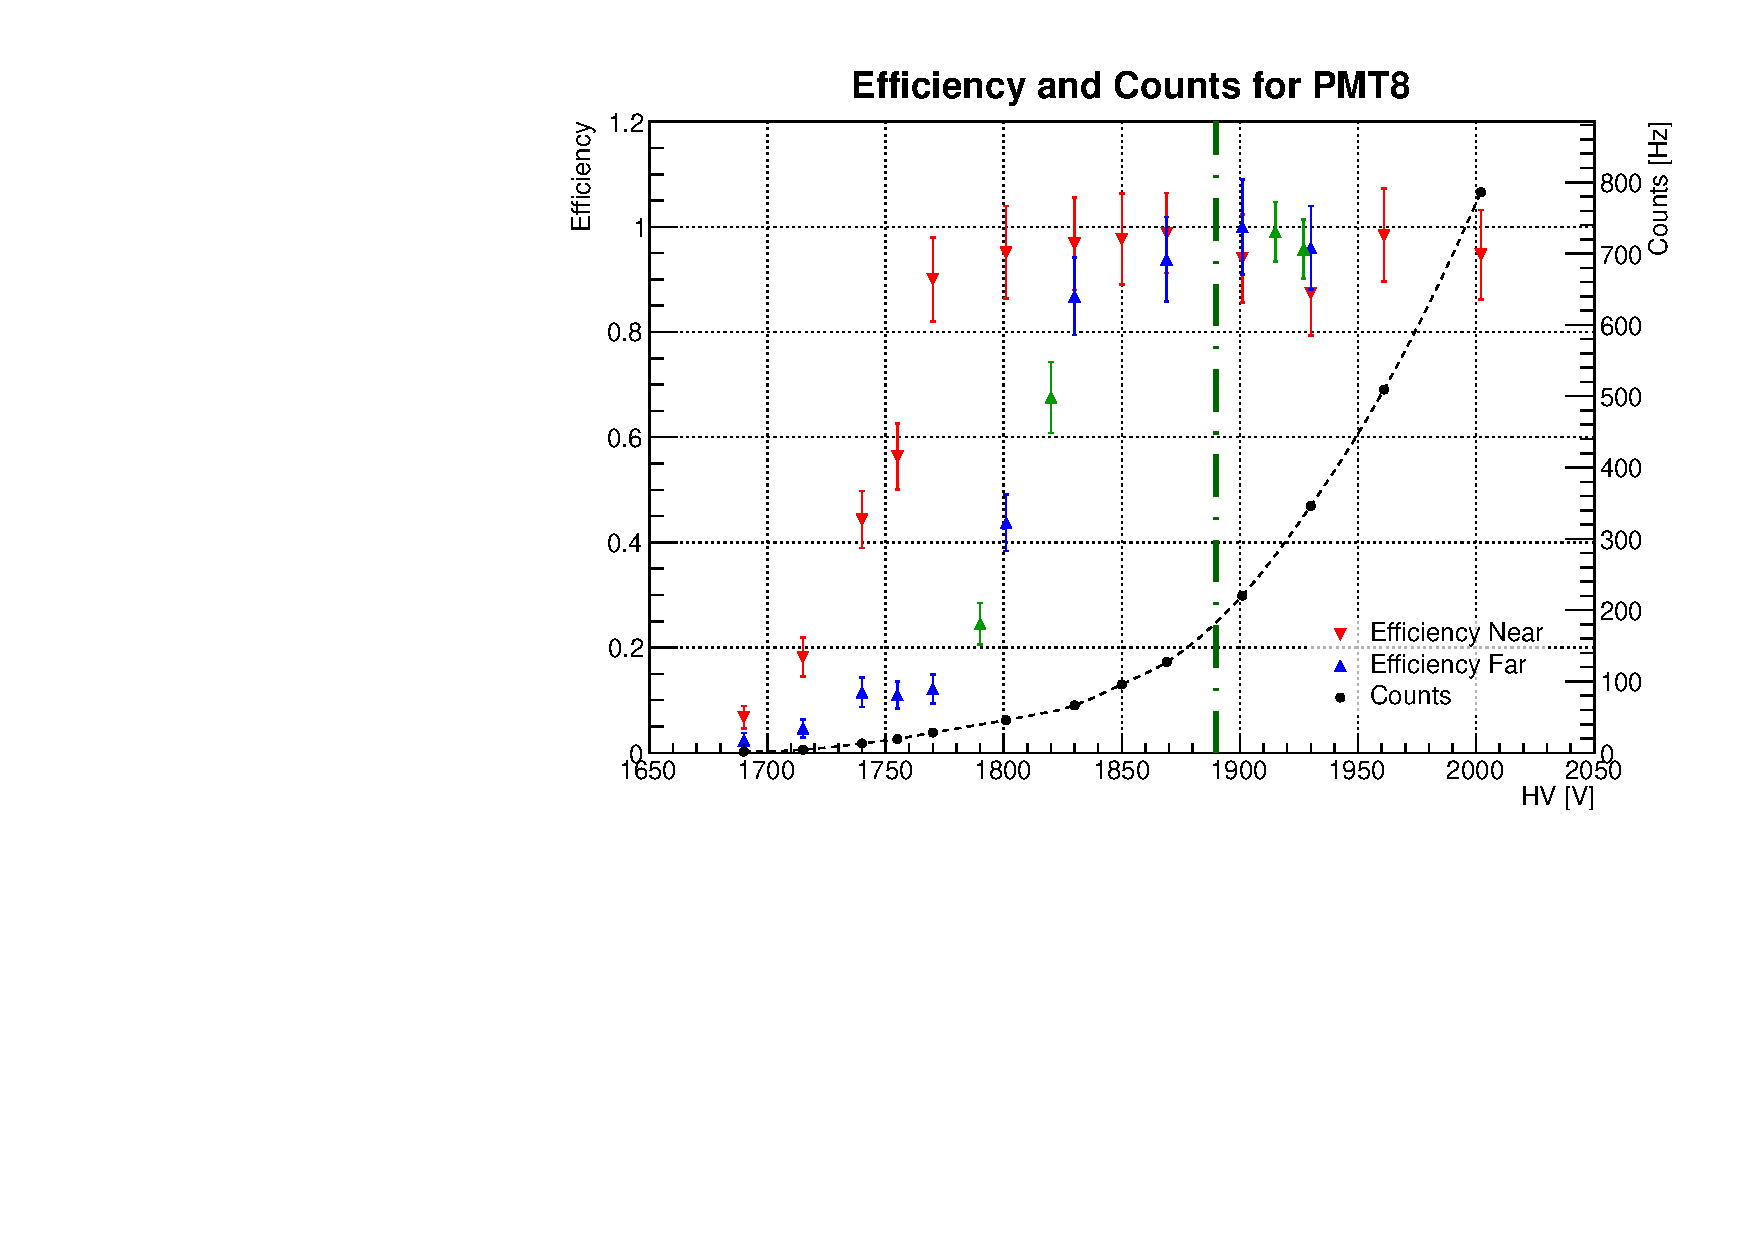
\includegraphics[scale=0.8]{img/eff8.pdf}}
\end{figure}
\begin{figure}[h]
	\centerline{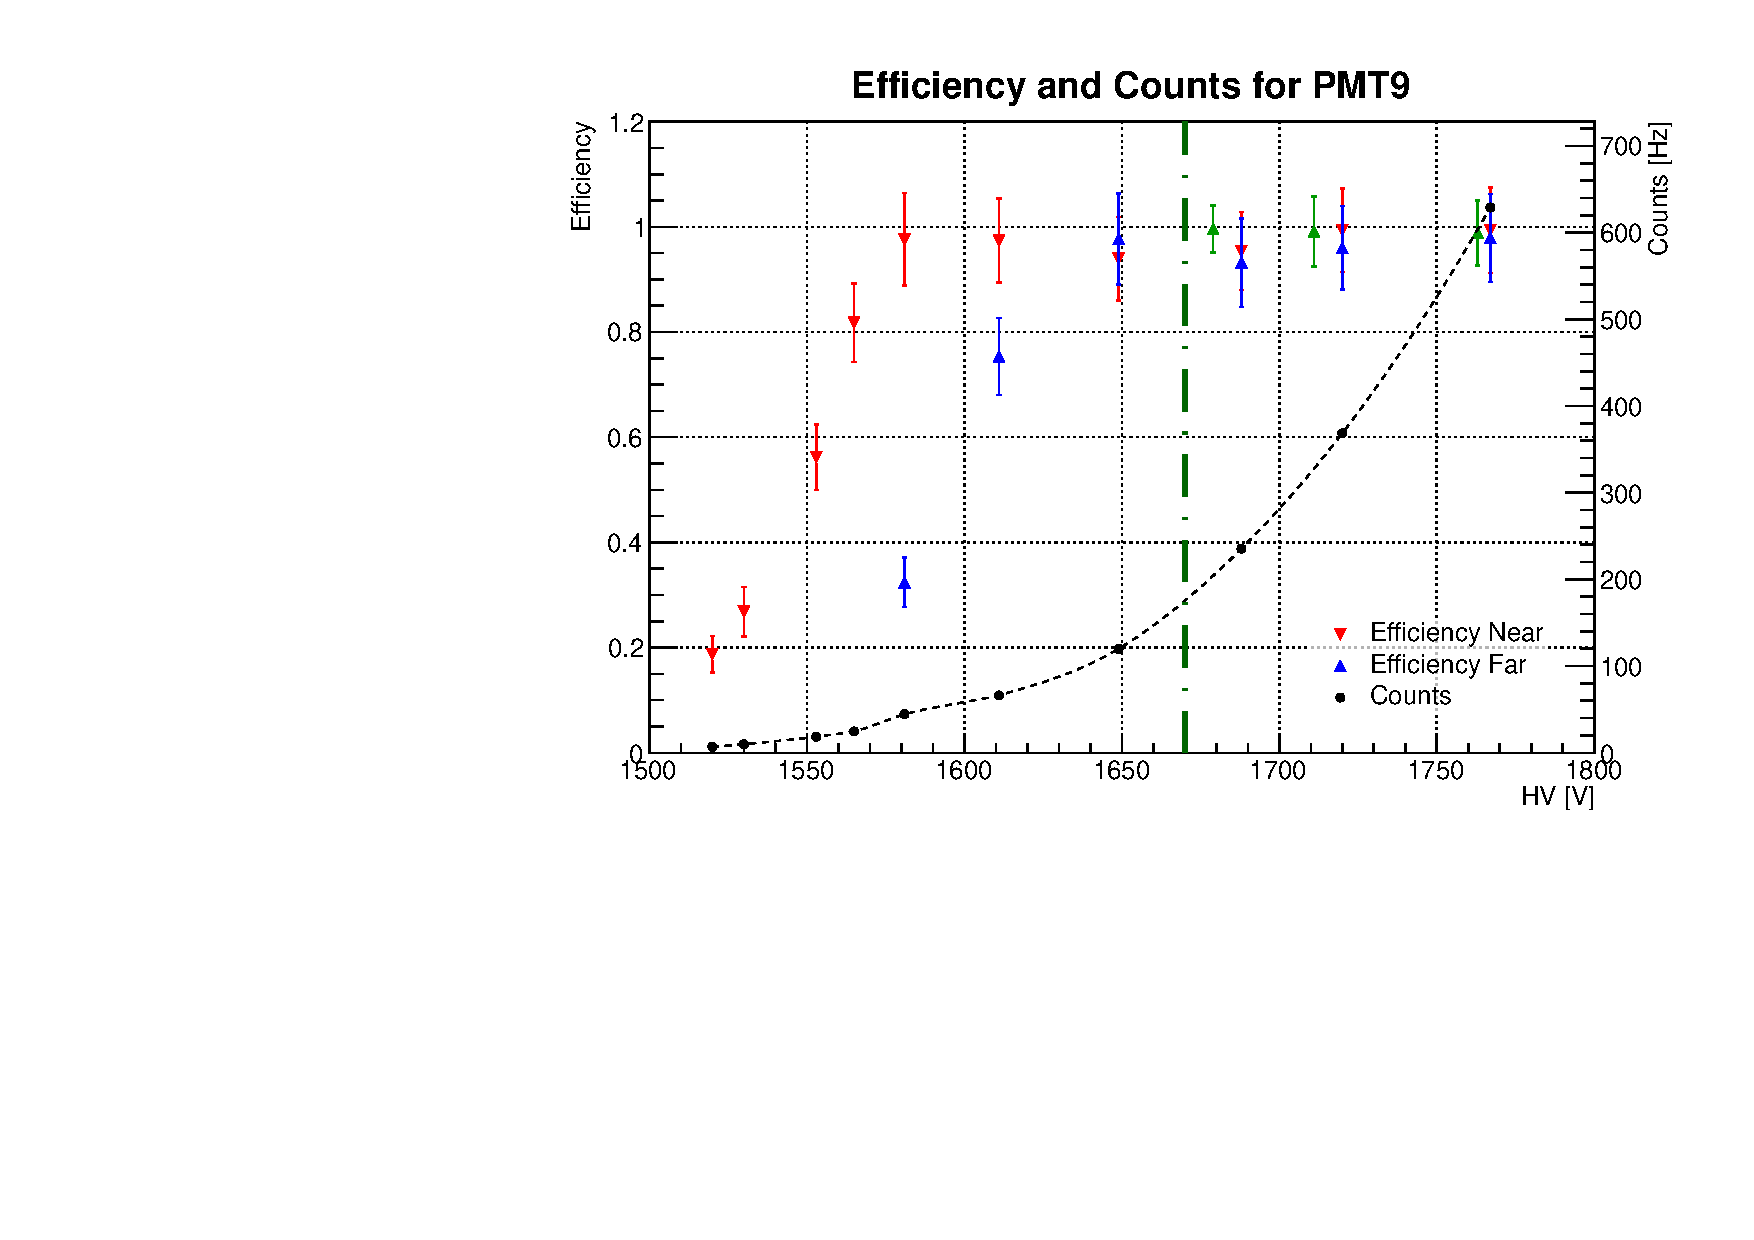
\includegraphics[scale=0.8]{img/eff9.pdf}}
\end{figure}
\begin{figure}[h]
	\centerline{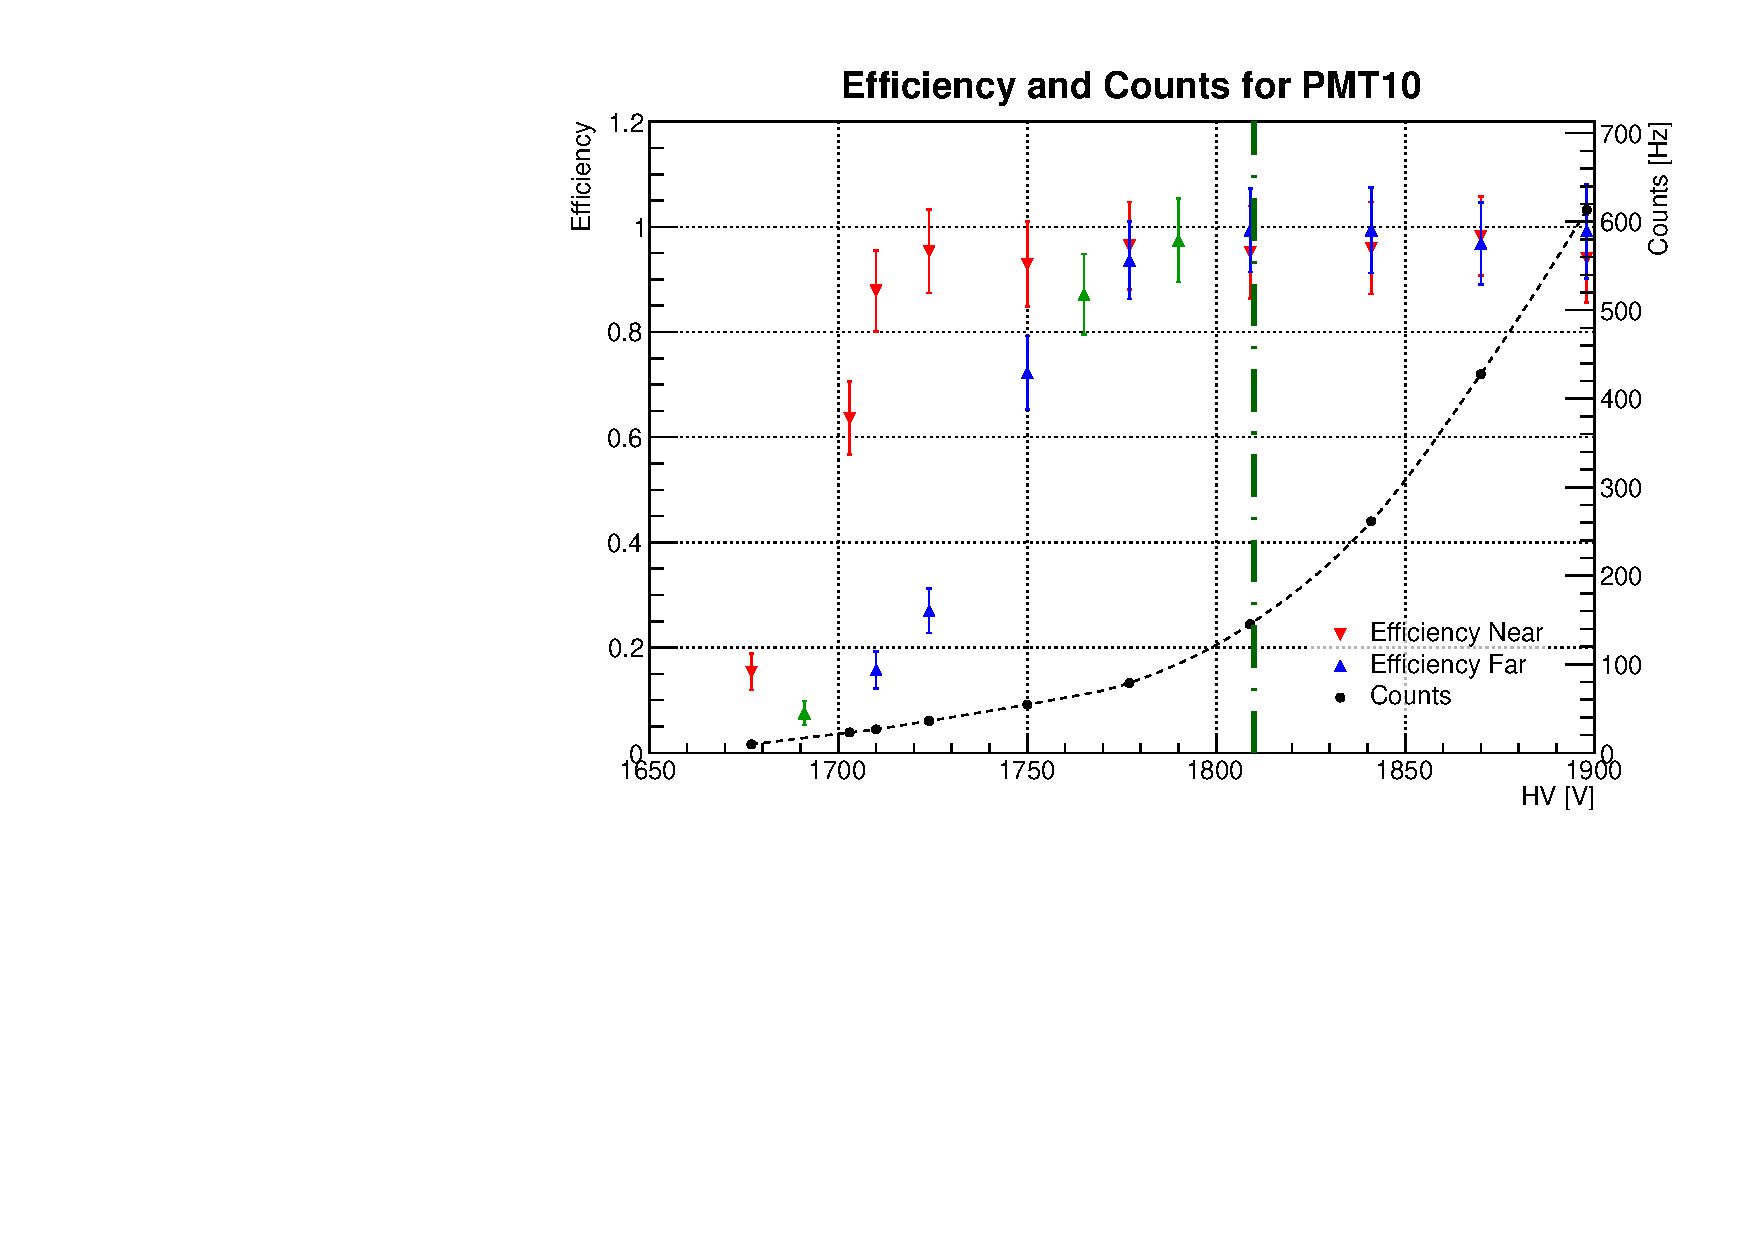
\includegraphics[scale=0.8]{img/eff10.pdf}}
\end{figure}
\begin{figure}[h]
	\centerline{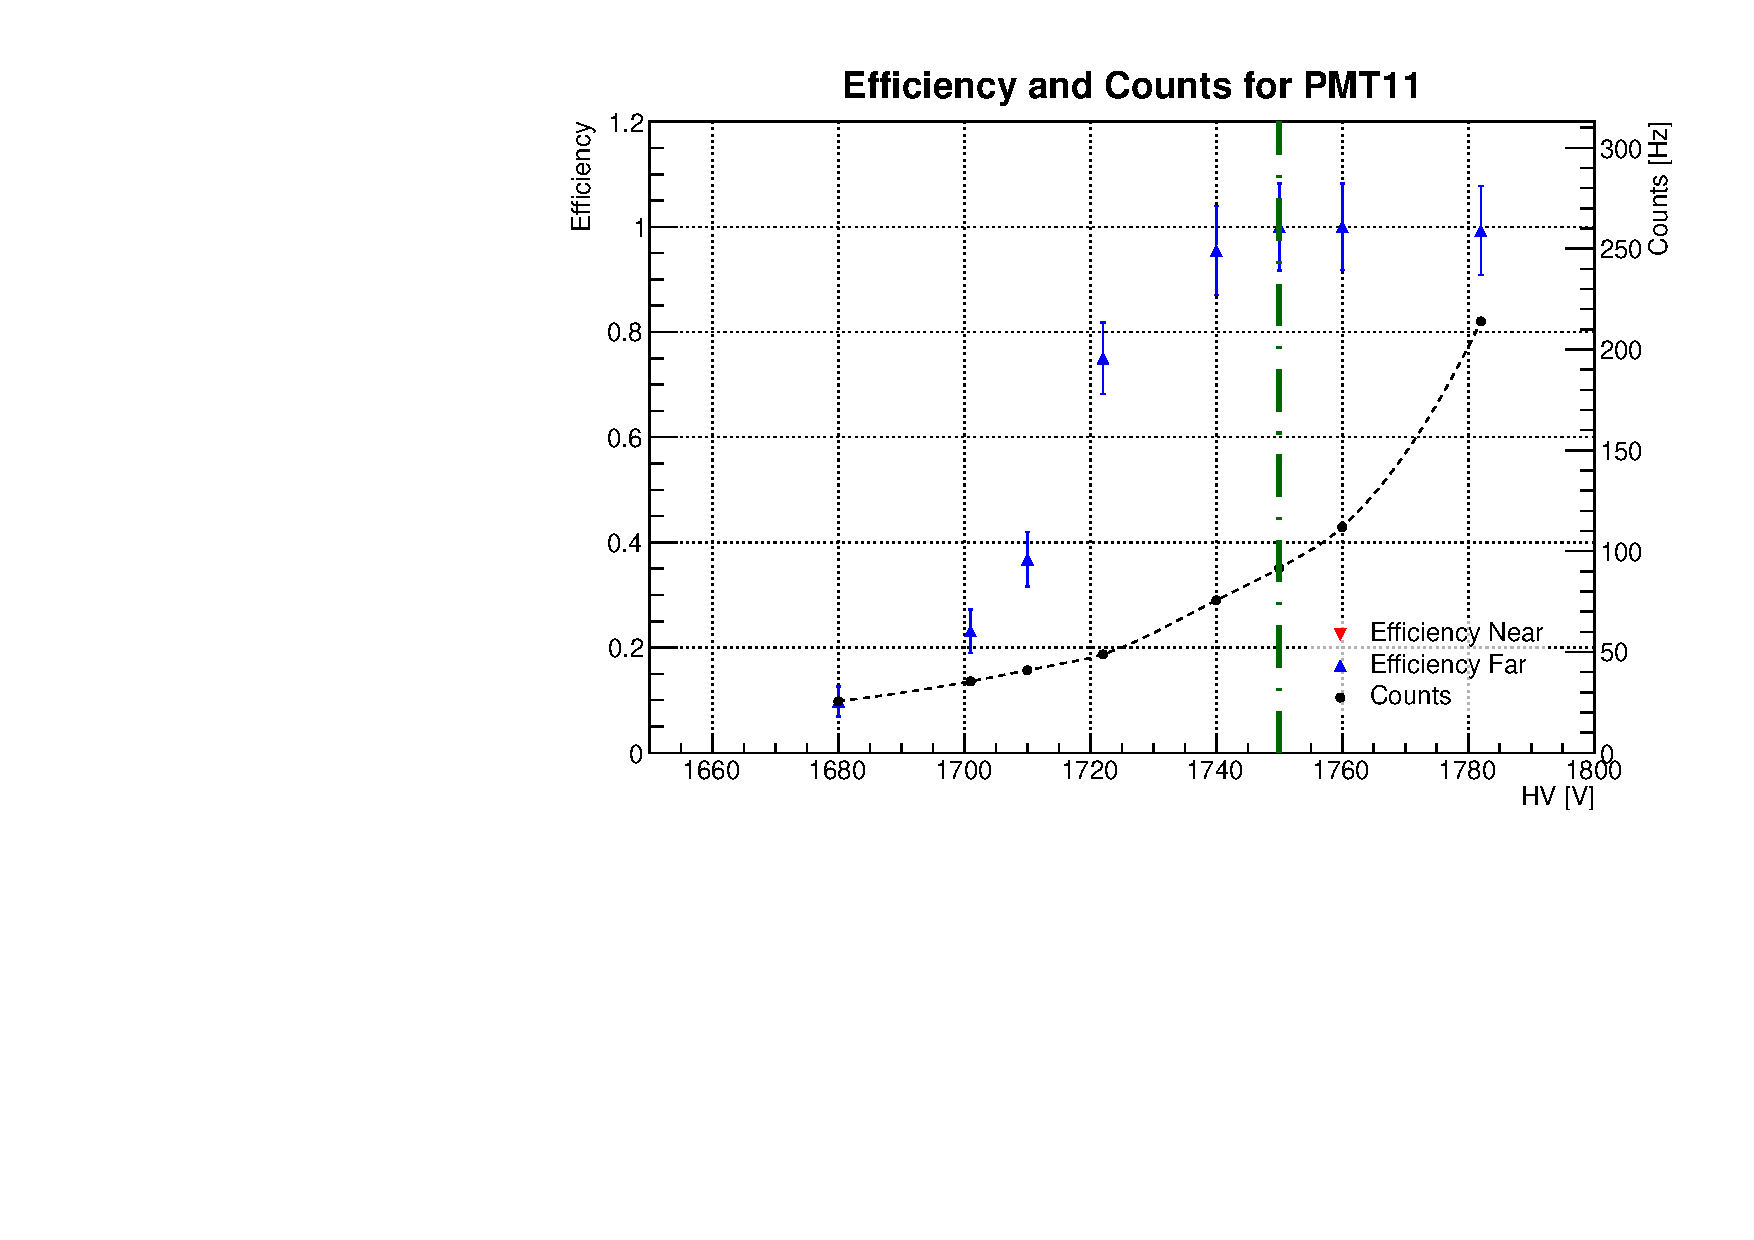
\includegraphics[scale=0.8]{img/eff11.pdf}}
\end{figure}
\begin{figure}[h]
	\centerline{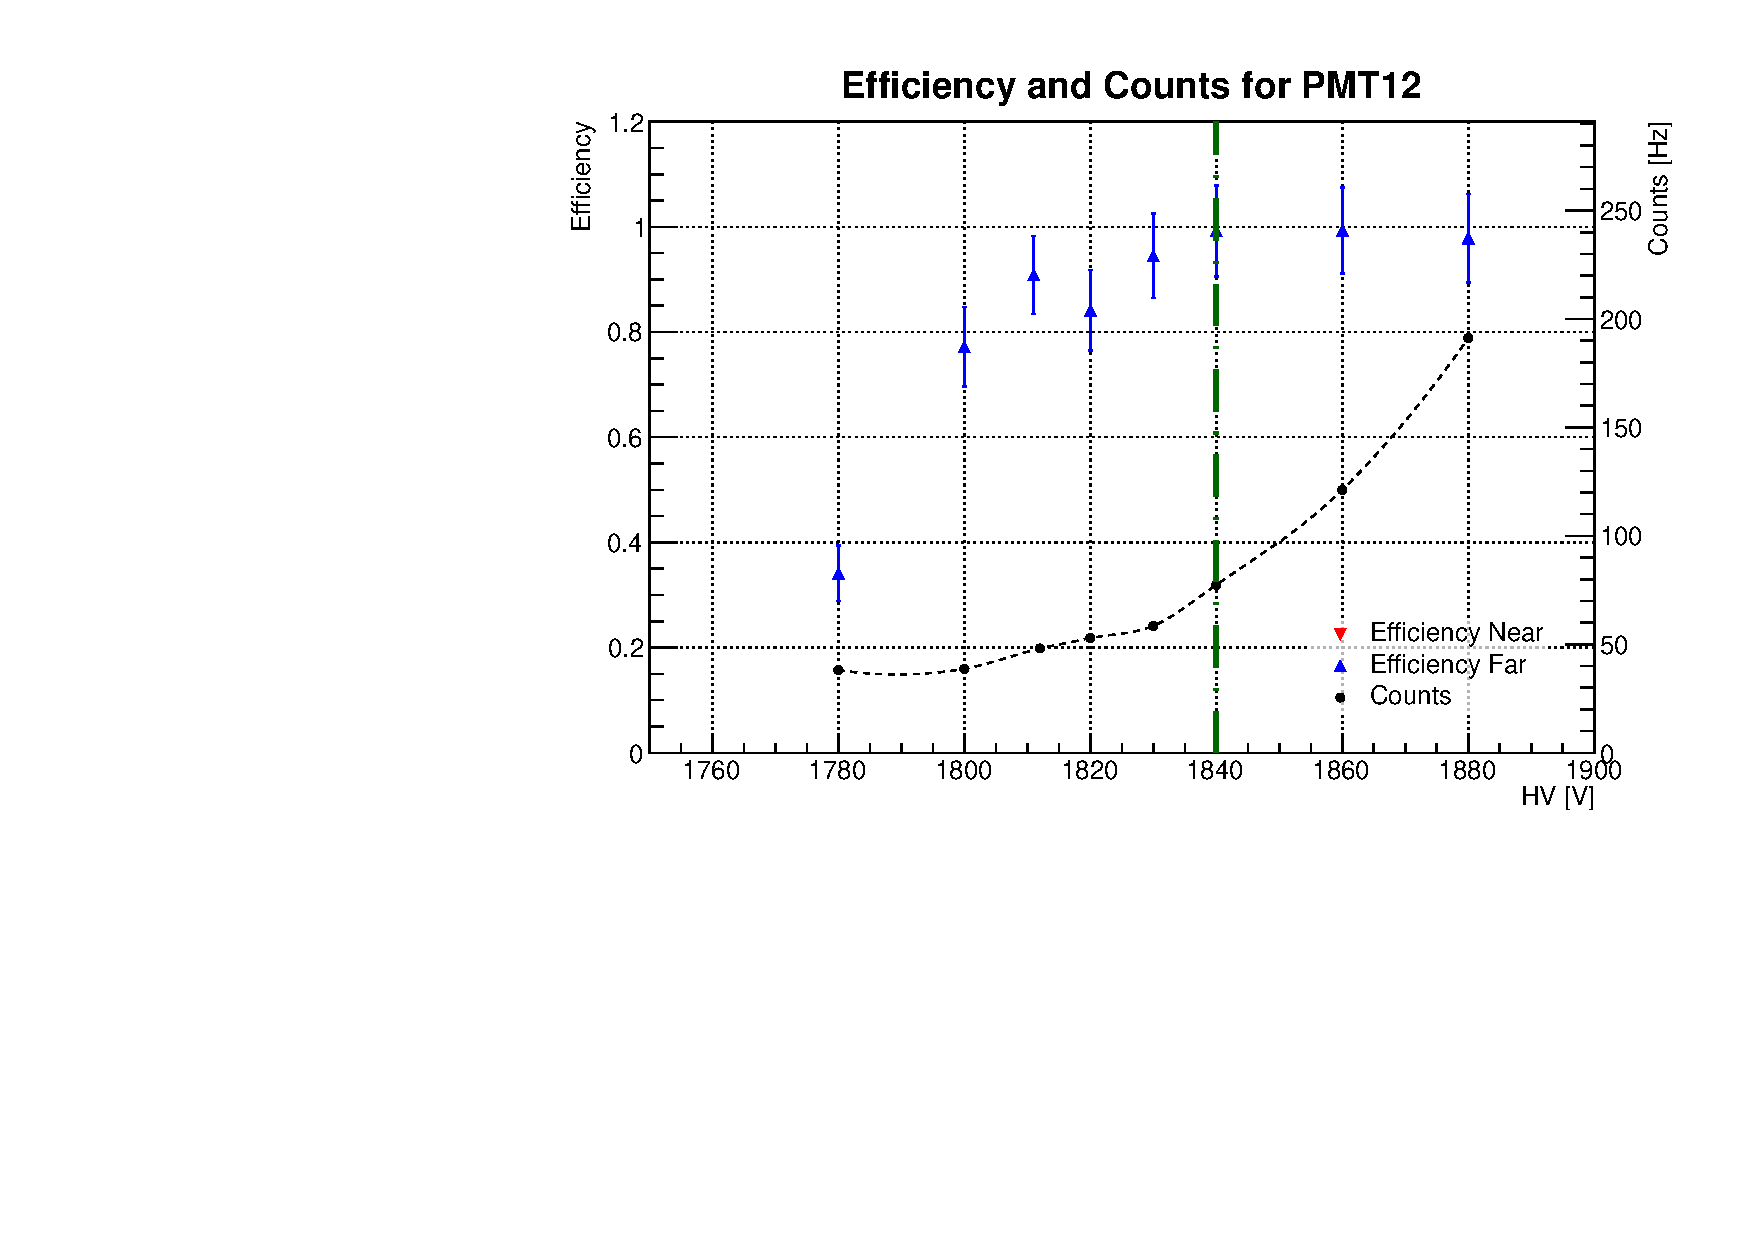
\includegraphics[scale=0.8]{img/eff12.pdf}}
\end{figure}
\begin{figure}[h]
	\centerline{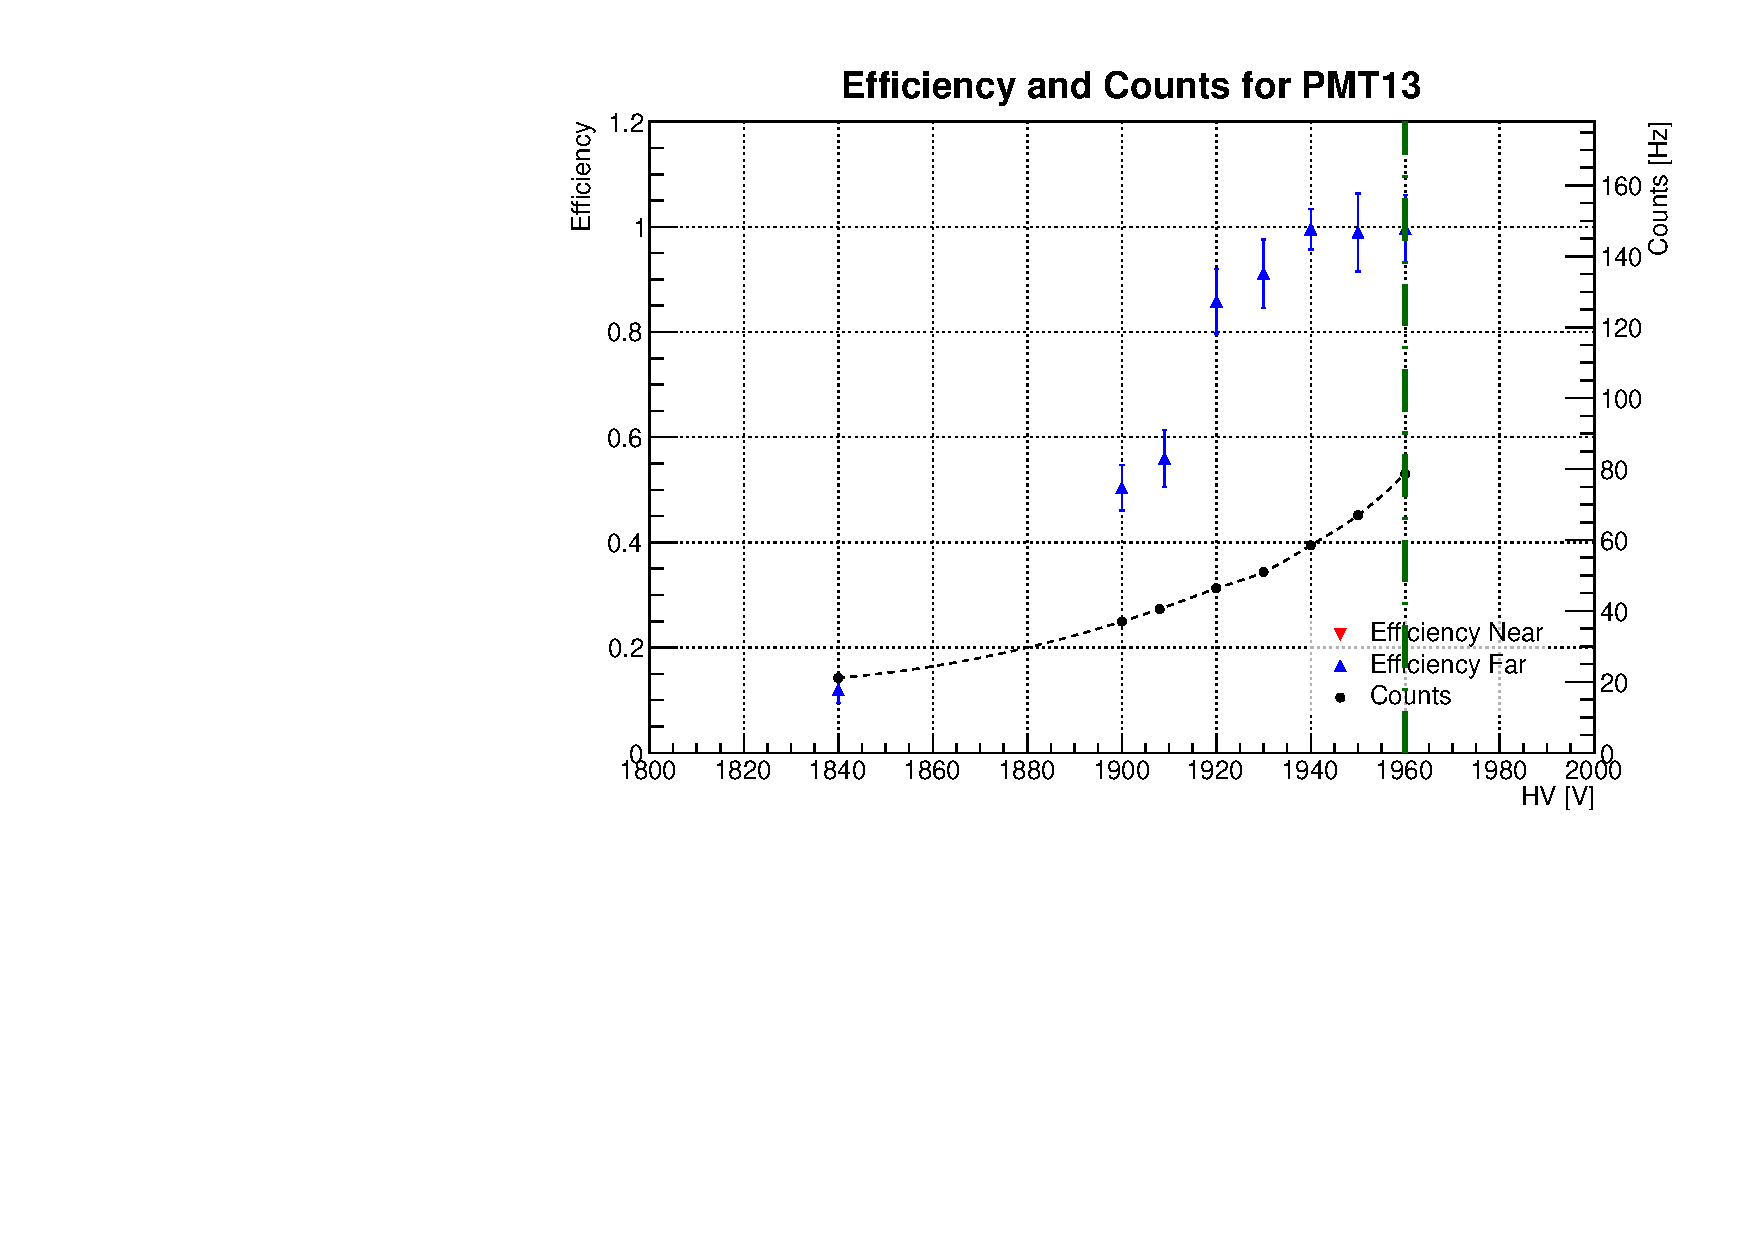
\includegraphics[scale=0.8]{img/eff13.pdf}}
\end{figure}
\begin{figure}[h]
	\centerline{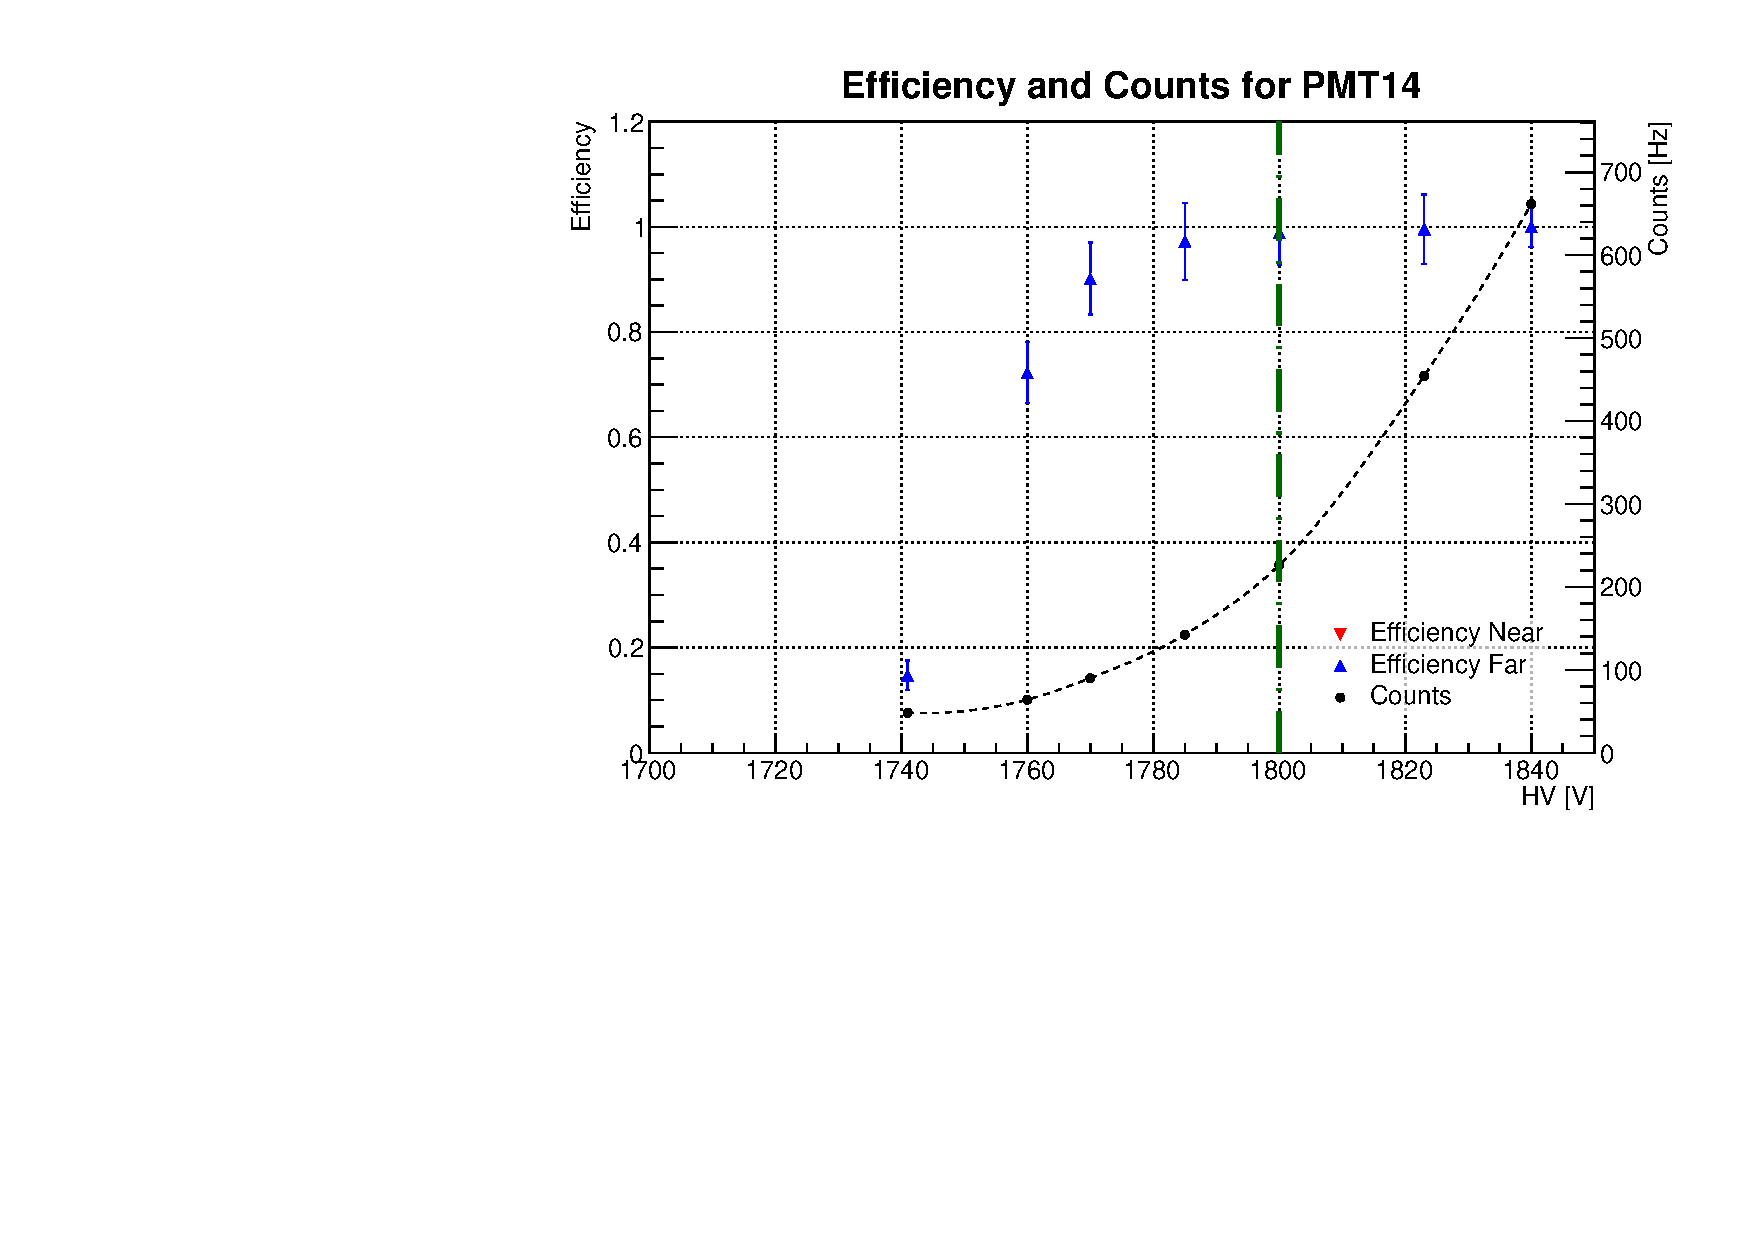
\includegraphics[scale=0.8]{img/eff14.pdf}}
\end{figure}
%\begin{figure}[h]
%	\centerline{
%		\subfloat
%		{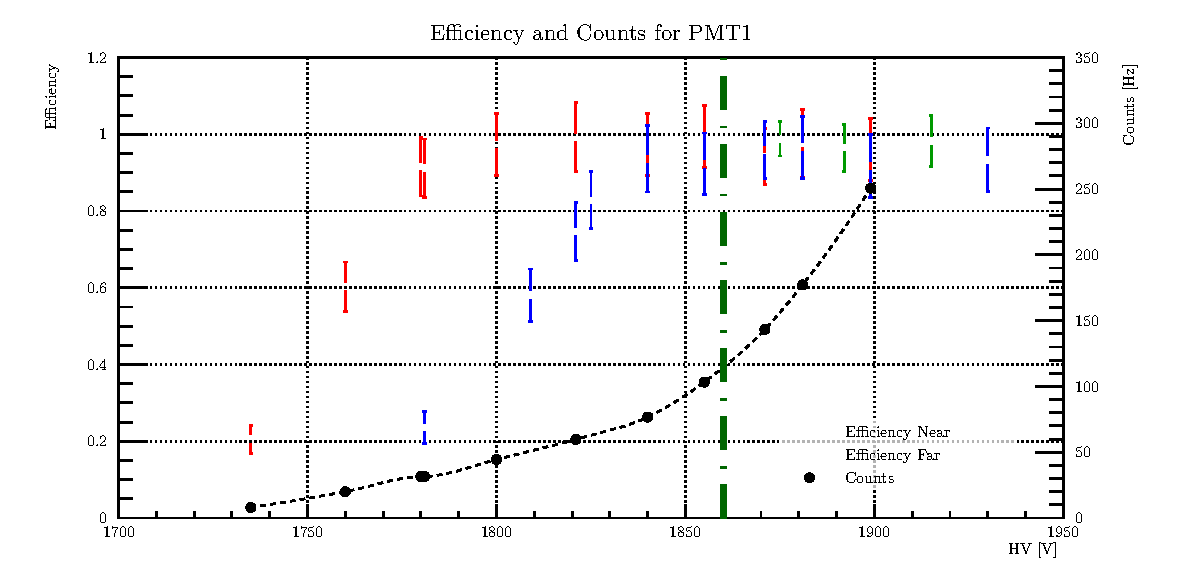
\includegraphics[scale=0.5]{img/eff1.pdf}}
%		\subfloat
%		{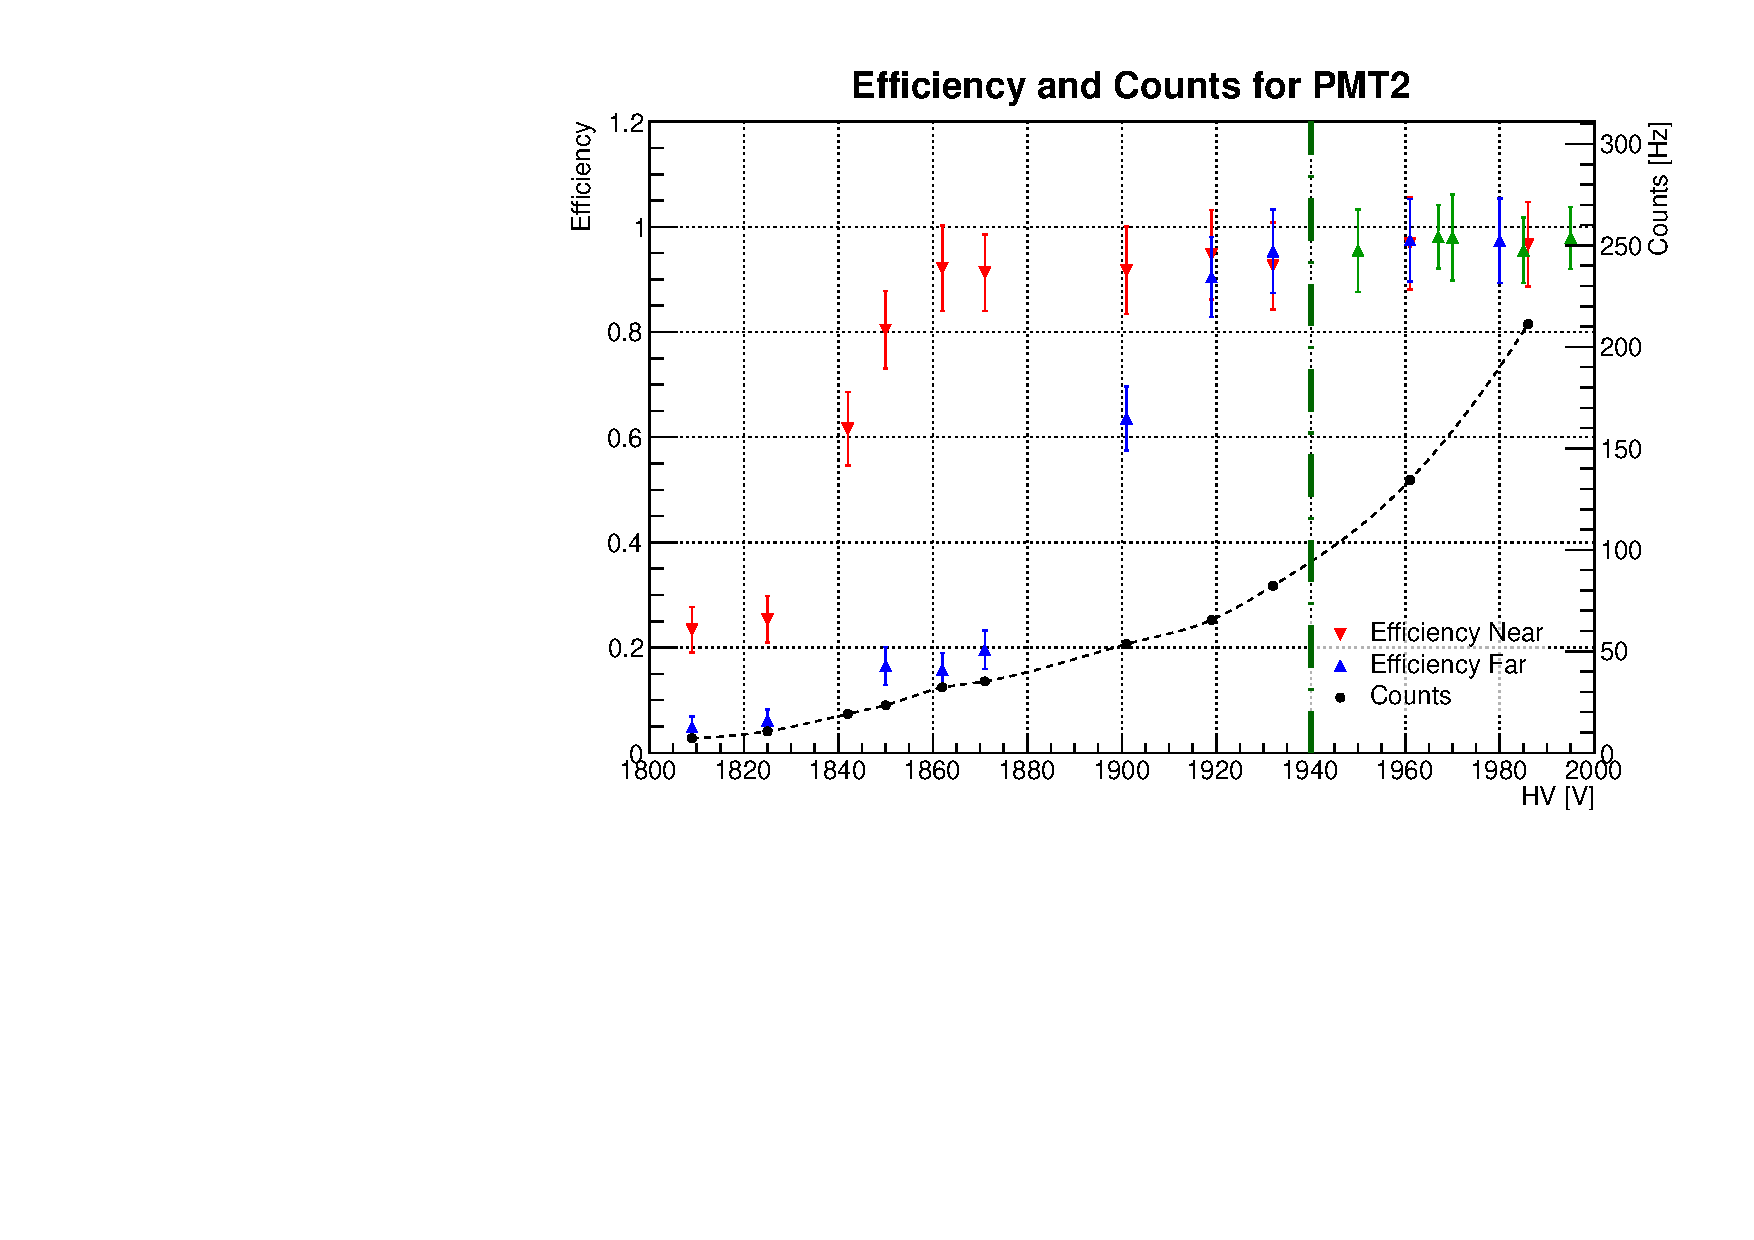
\includegraphics[scale=0.5]{img/eff2.pdf}}}
%	\centerline{
%		\subfloat
%		{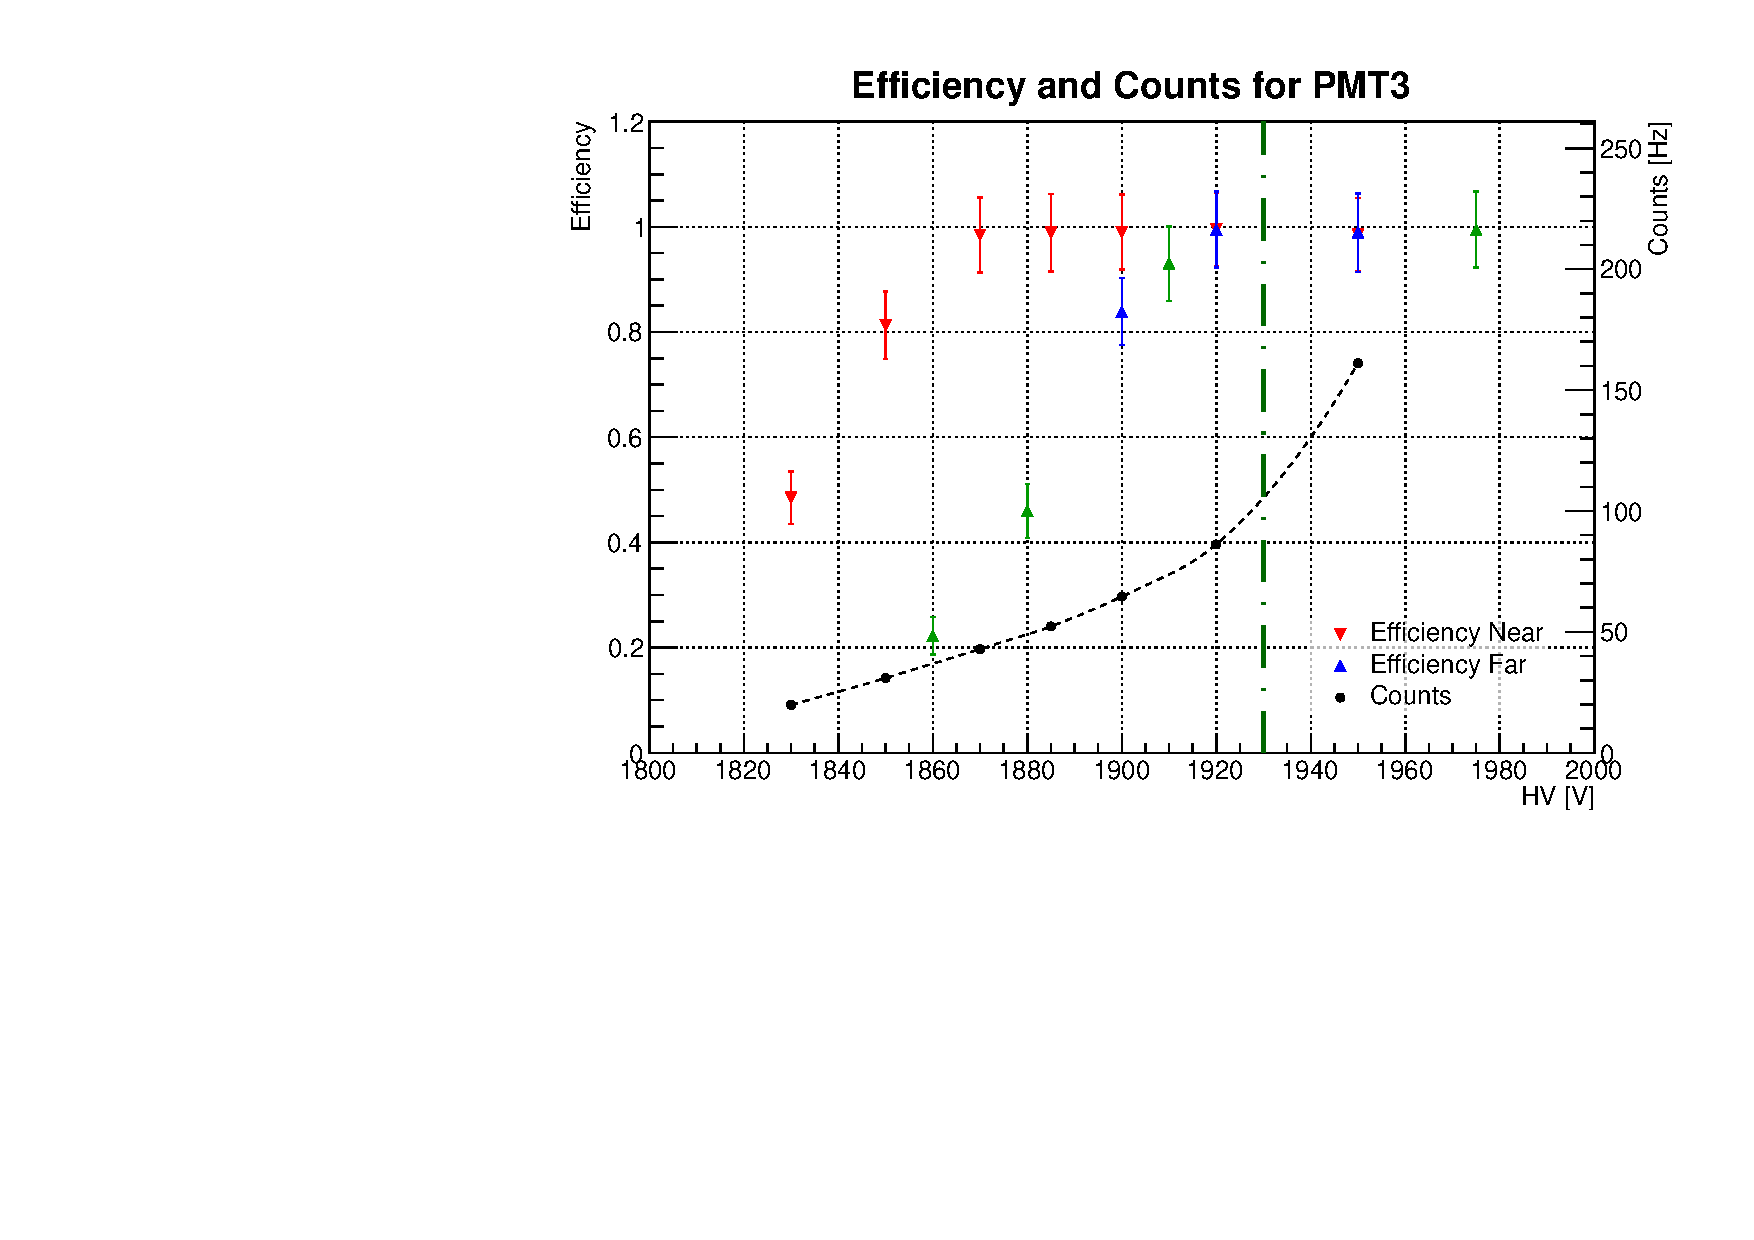
\includegraphics[scale=0.5]{img/eff3.pdf}}
%		\subfloat
%		{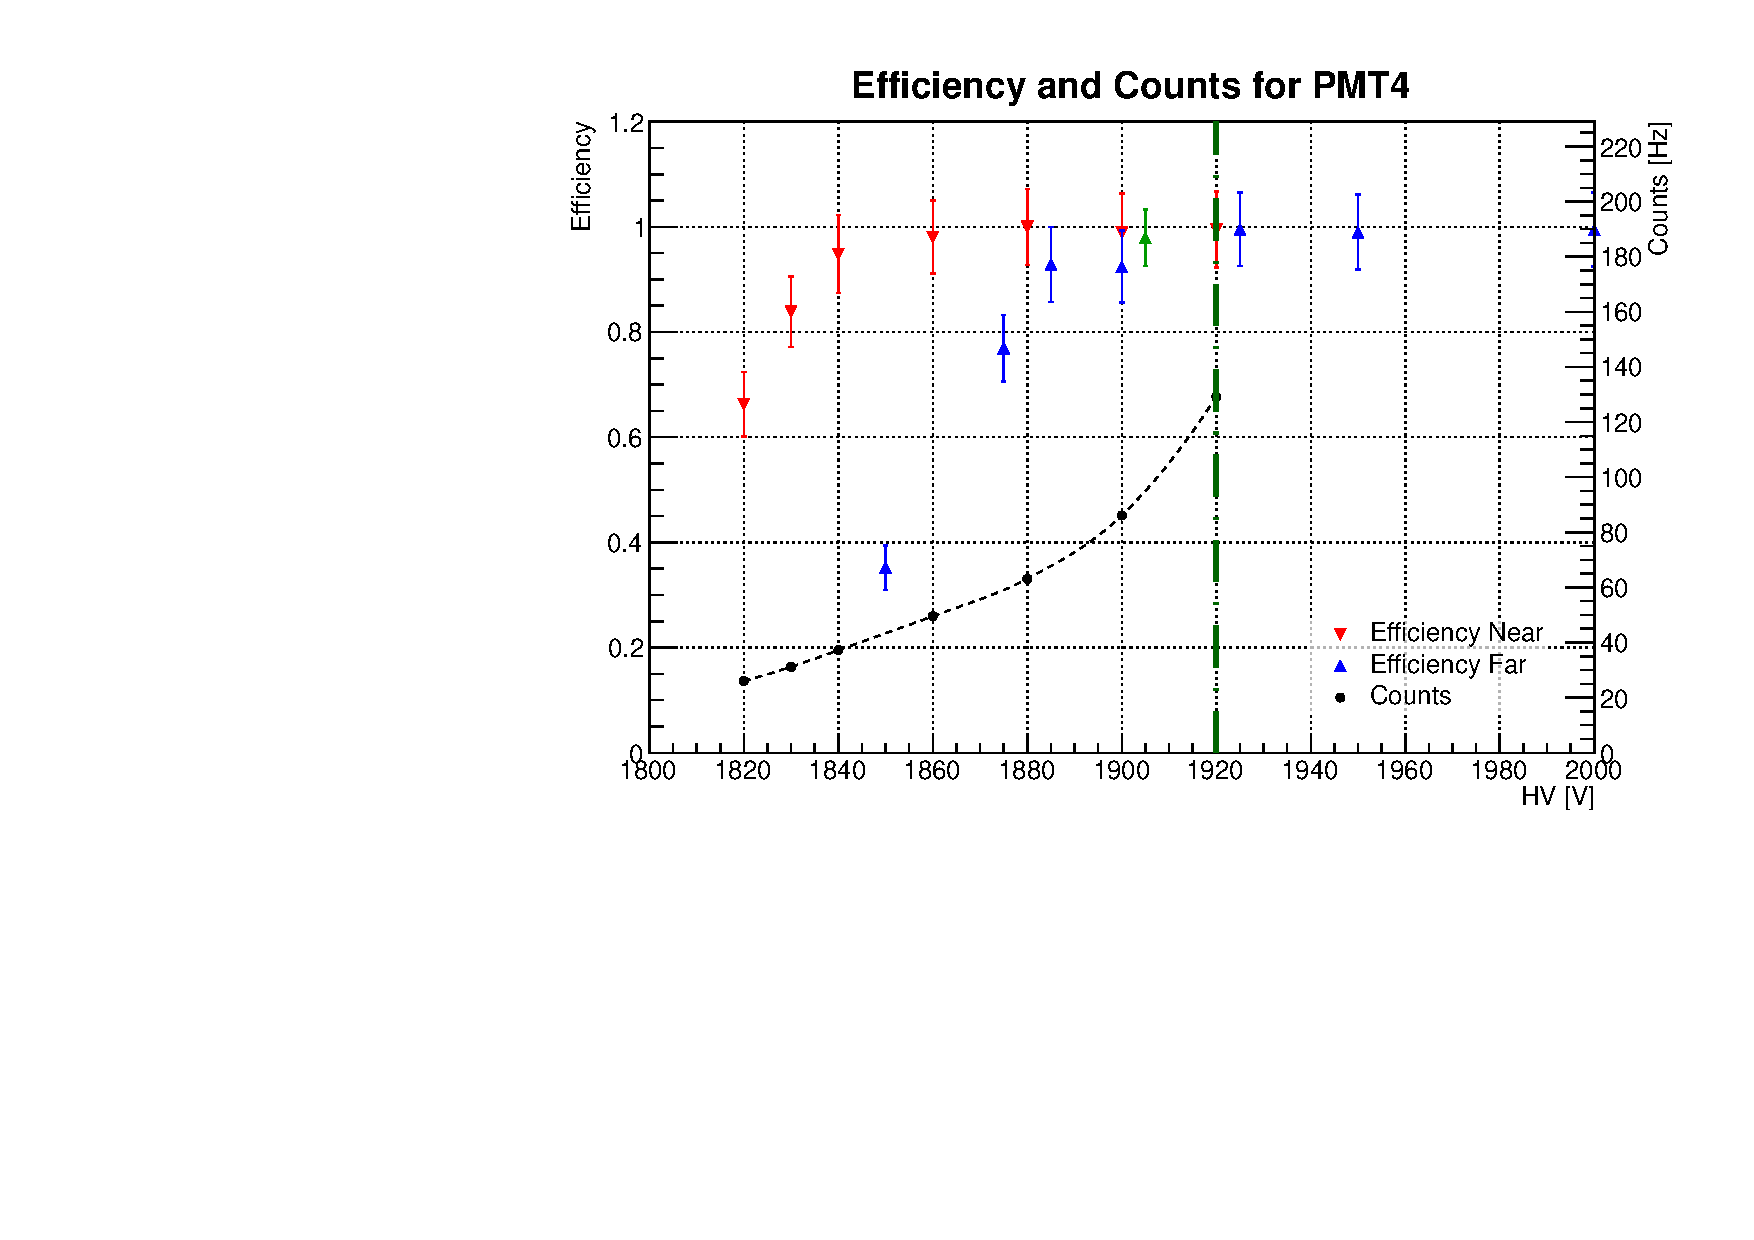
\includegraphics[scale=0.5]{img/eff4.pdf}}}
%\end{figure}
%\begin{figure}[h]
%	\centerline{
%		\subfloat
%		{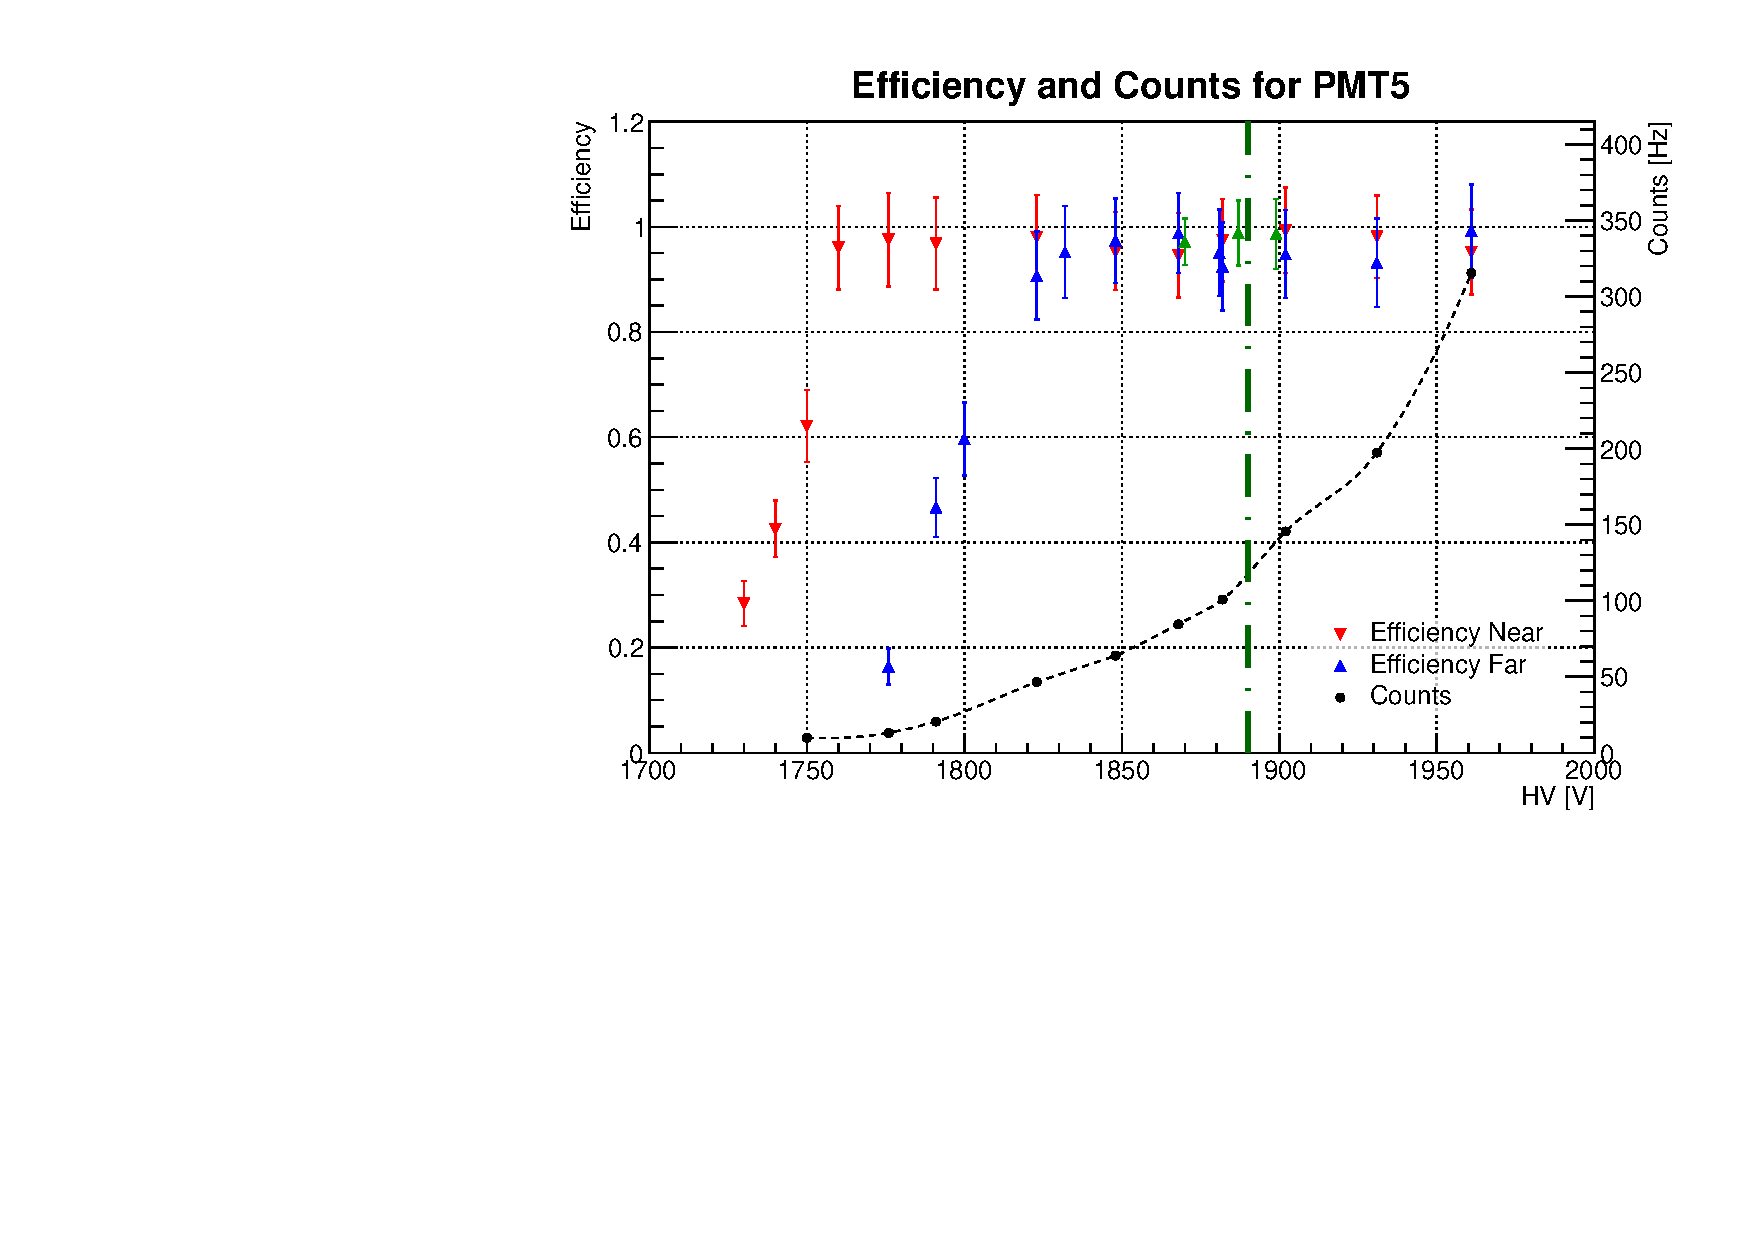
\includegraphics[scale=0.5]{img/eff5.pdf}}
%		\subfloat
%		{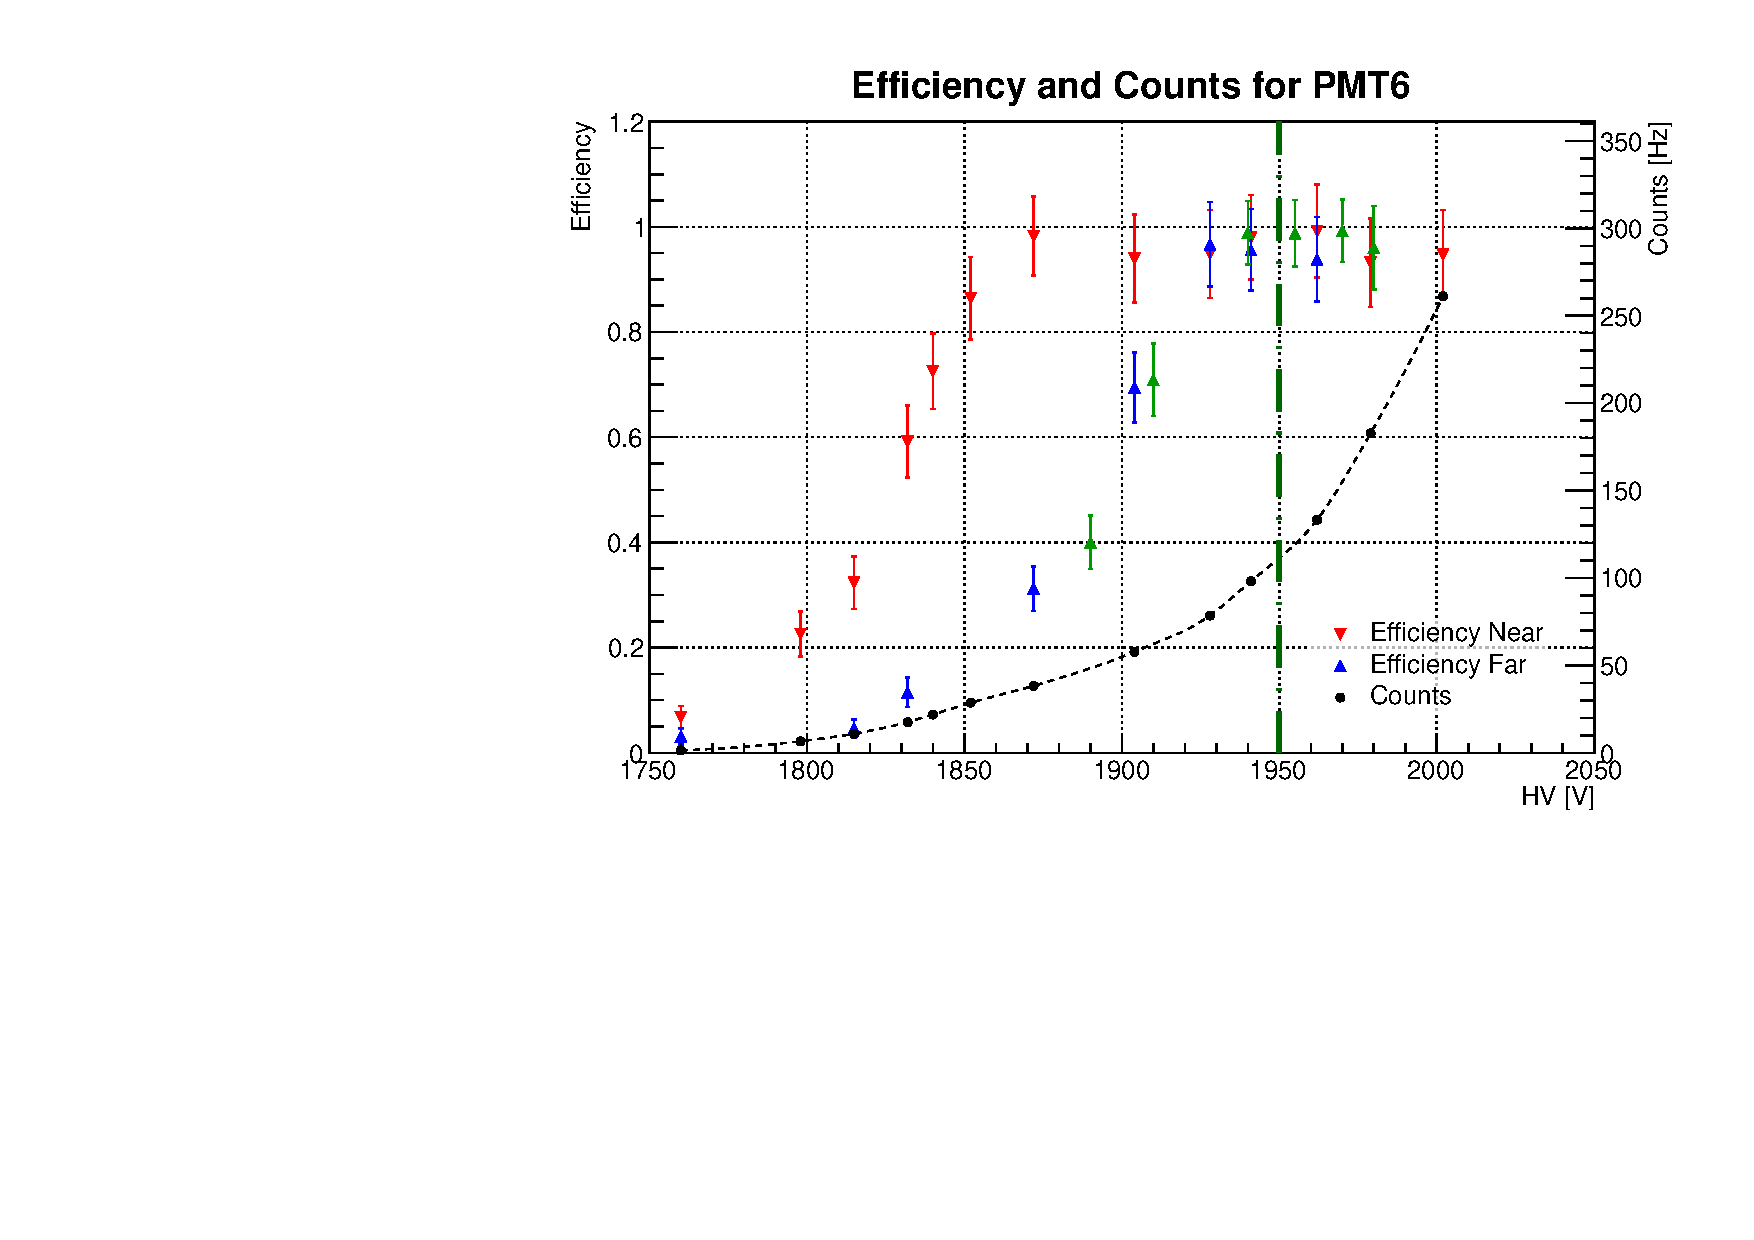
\includegraphics[scale=0.5]{img/eff6.pdf}}}
%	\centerline{
%		\subfloat
%		{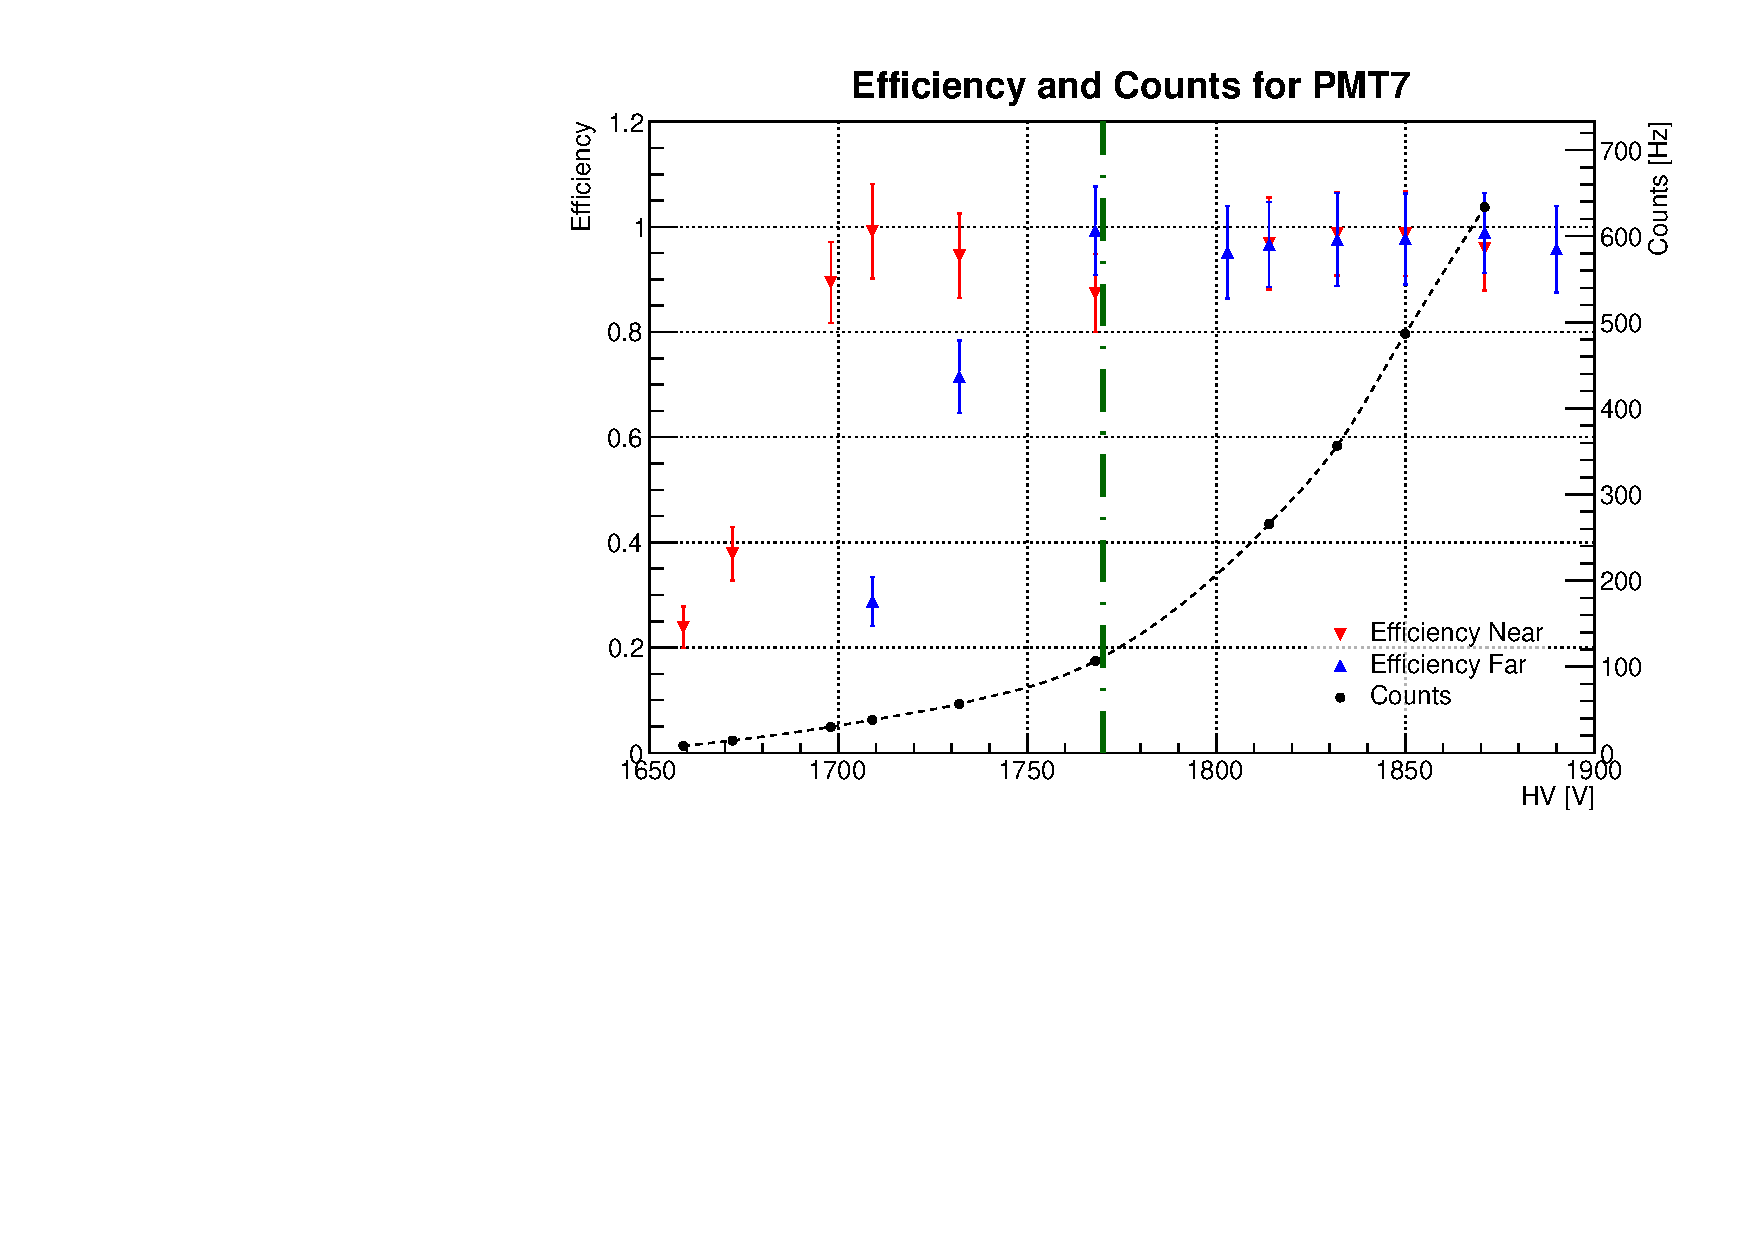
\includegraphics[scale=0.5]{img/eff7.pdf}}
%		\subfloat
%		{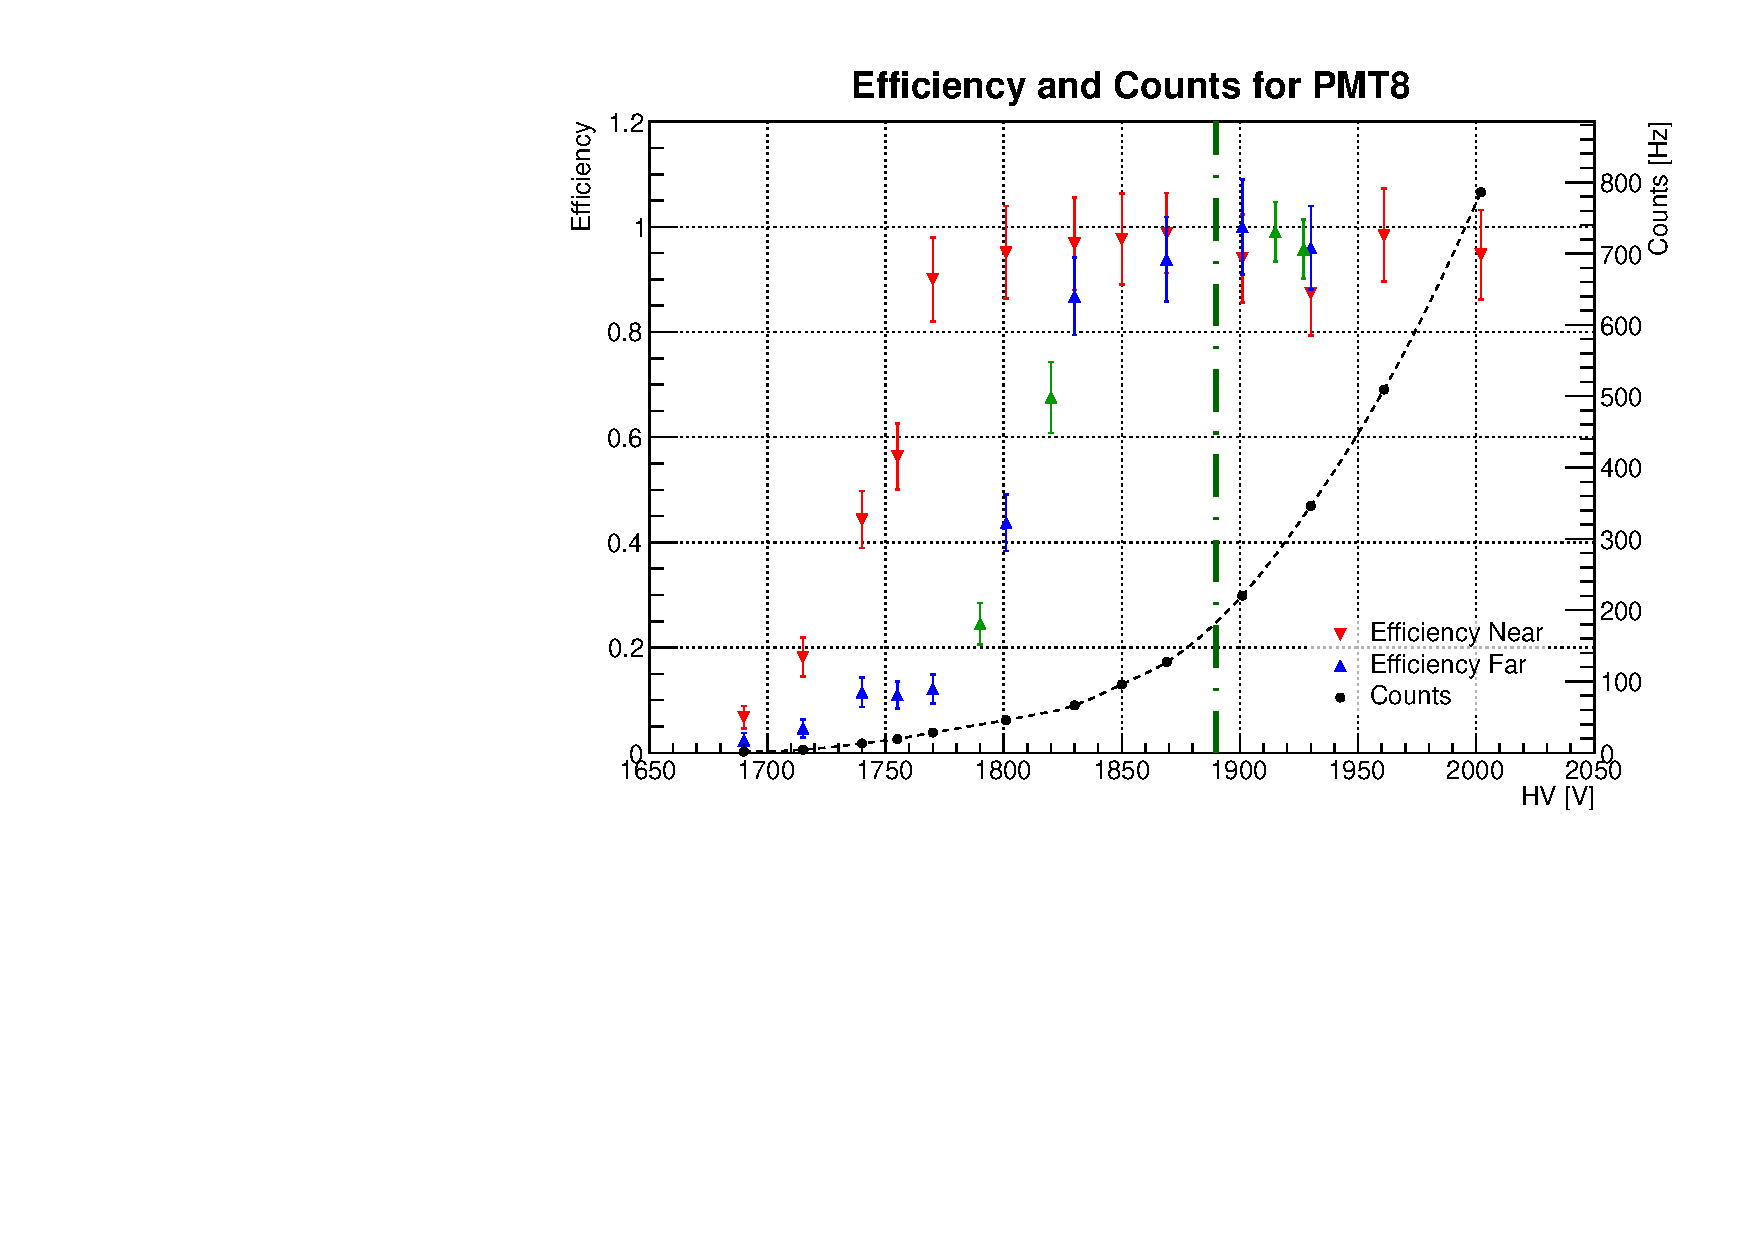
\includegraphics[scale=0.5]{img/eff8.pdf}}}
%\end{figure}
%\begin{figure}[h]
%	\centerline{
%		\subfloat
%		{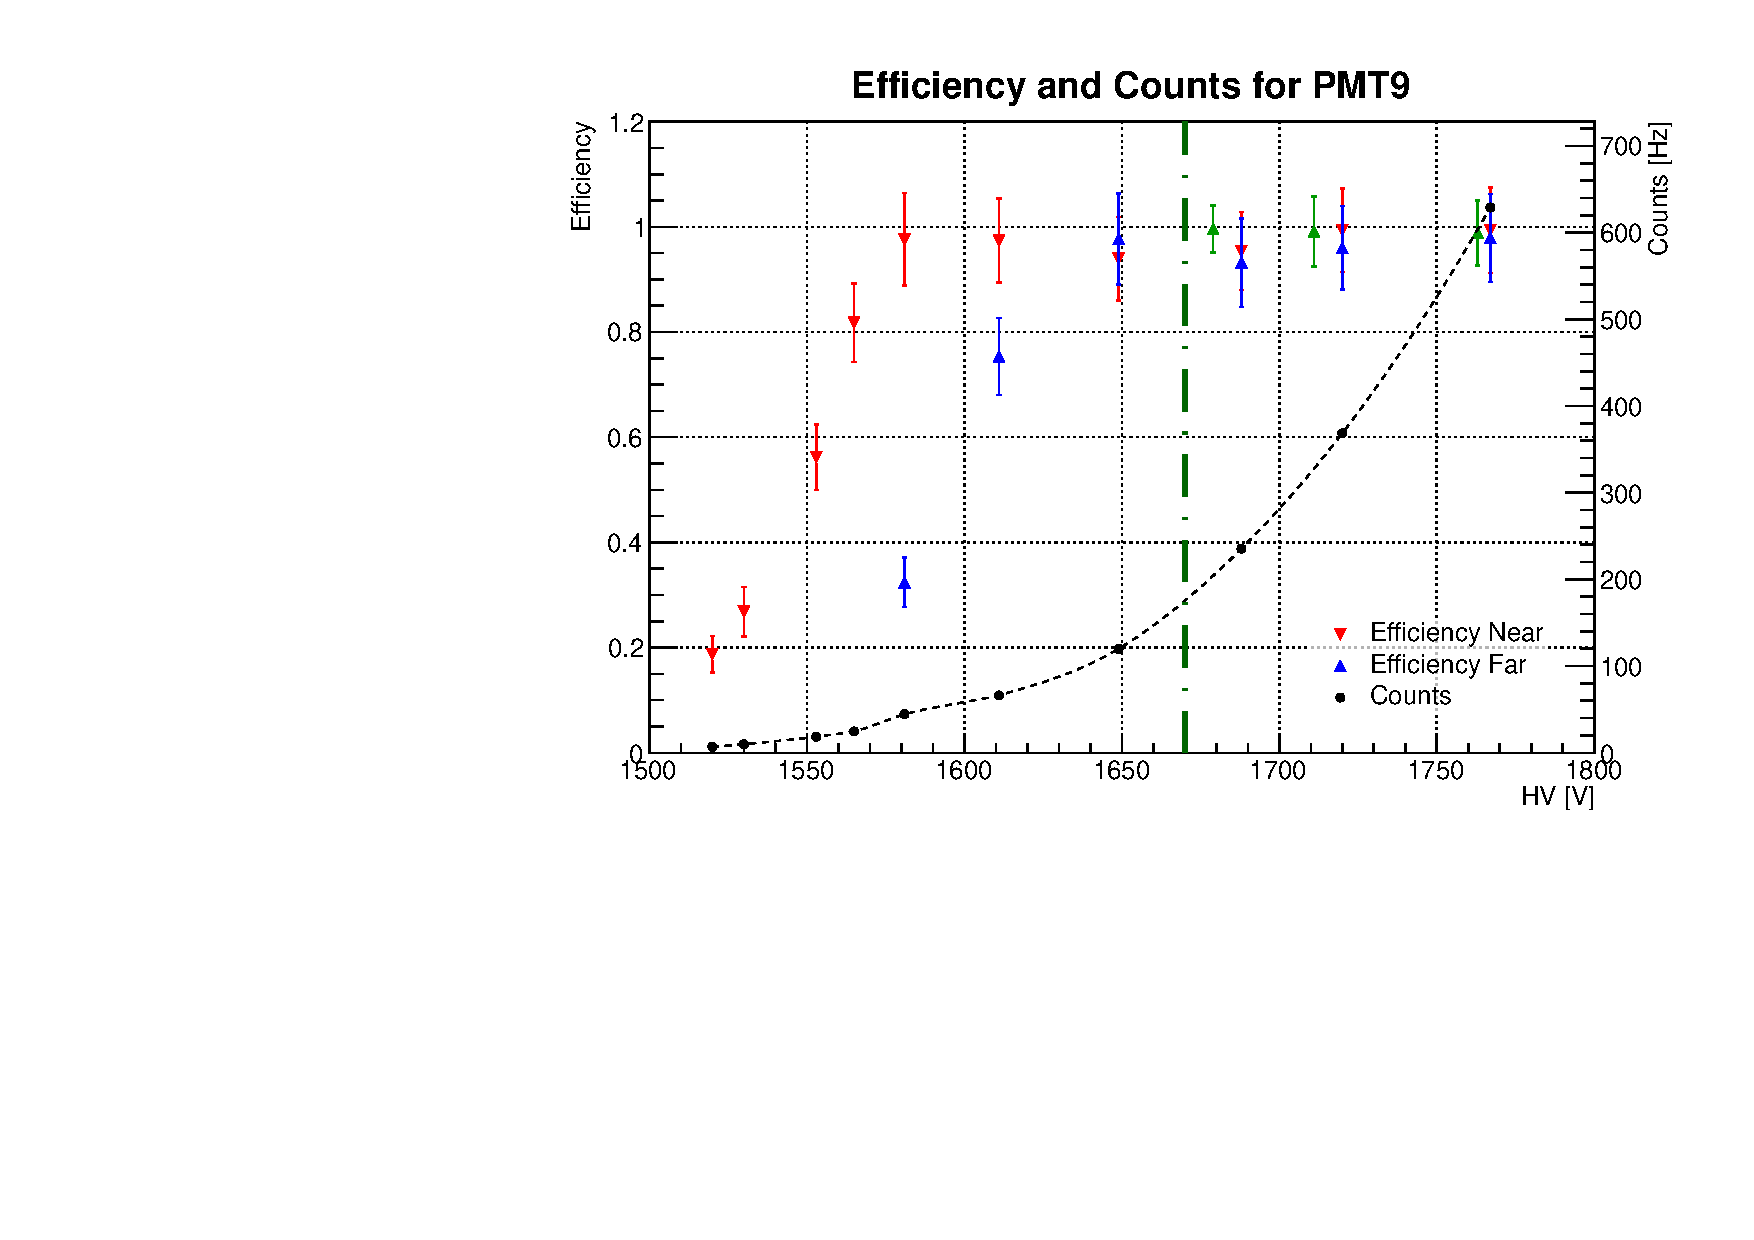
\includegraphics[scale=0.5]{img/eff9.pdf}}
%		\subfloat
%		{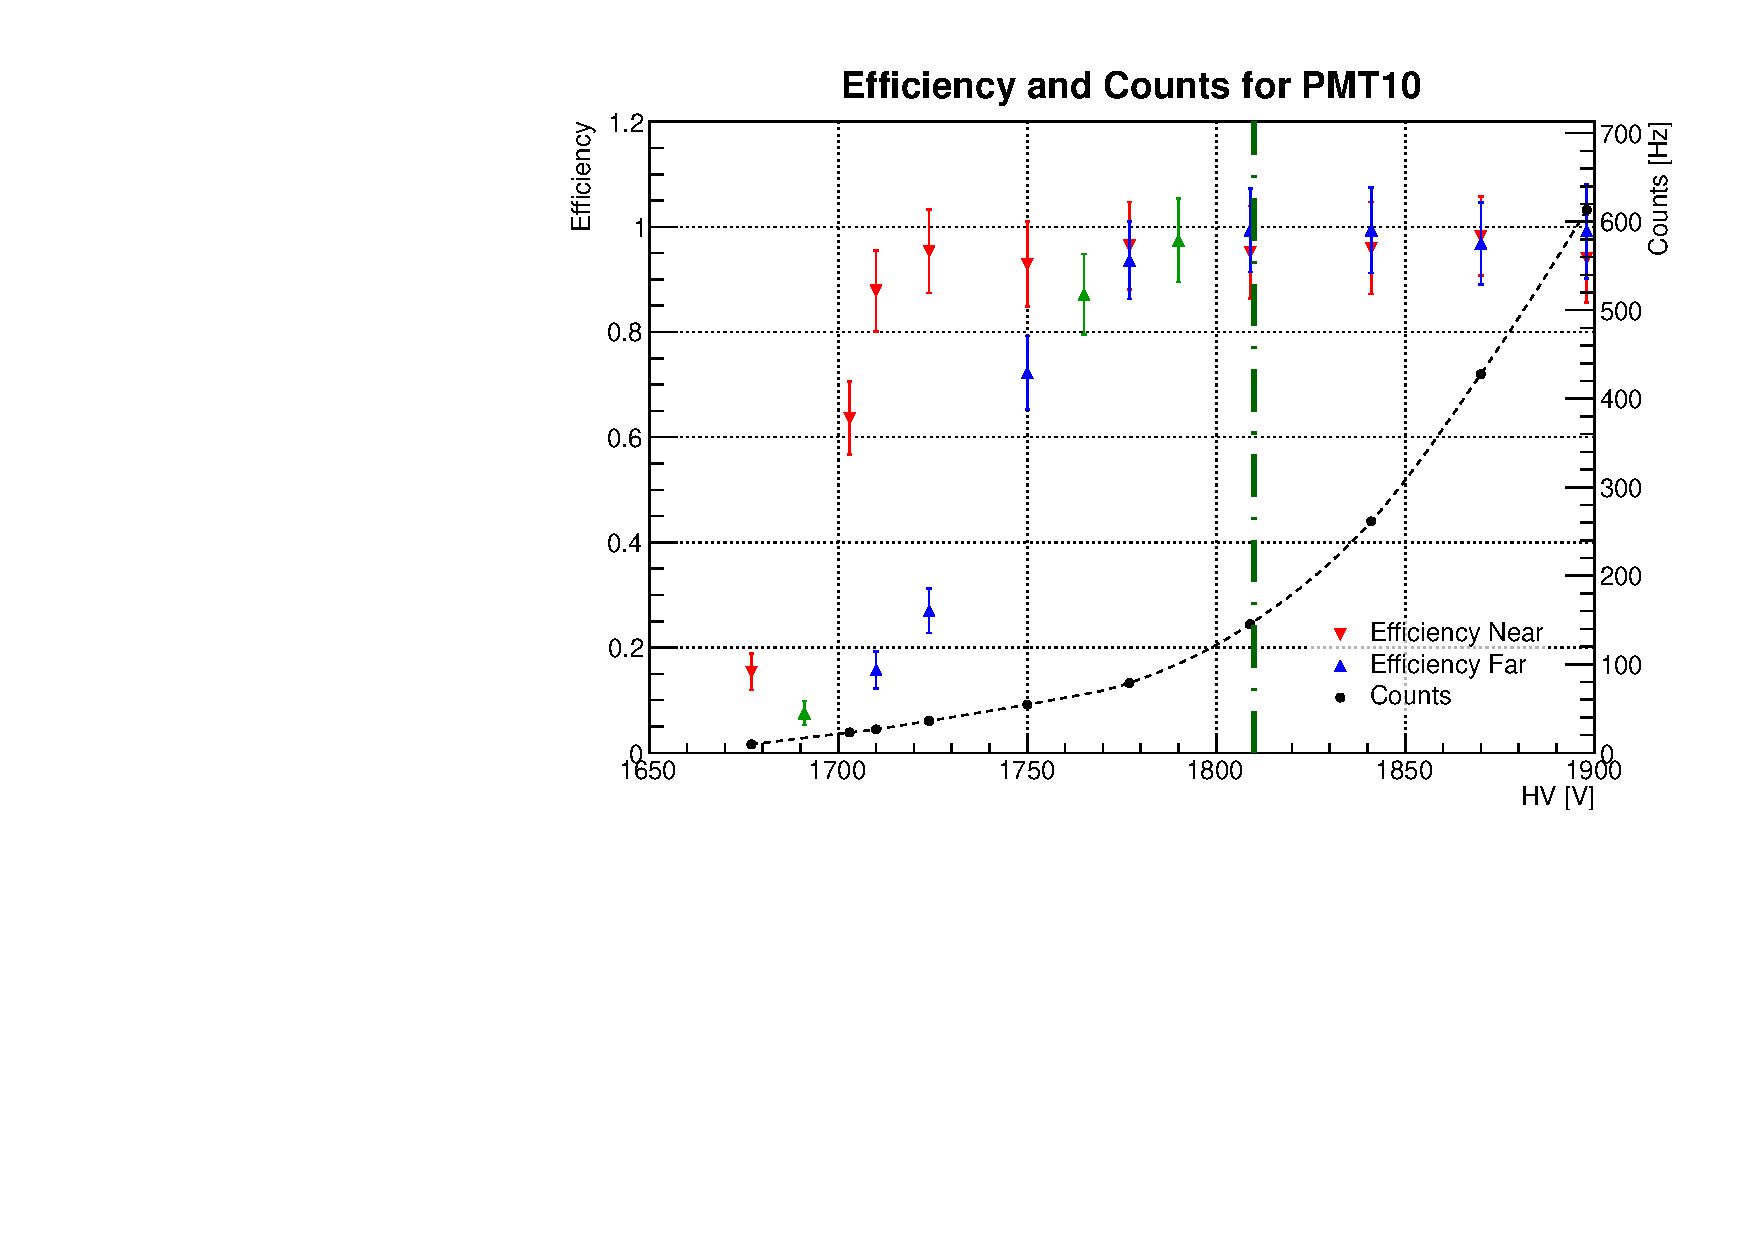
\includegraphics[scale=0.5]{img/eff10.pdf}}}
%	\centerline{
%		\subfloat
%		{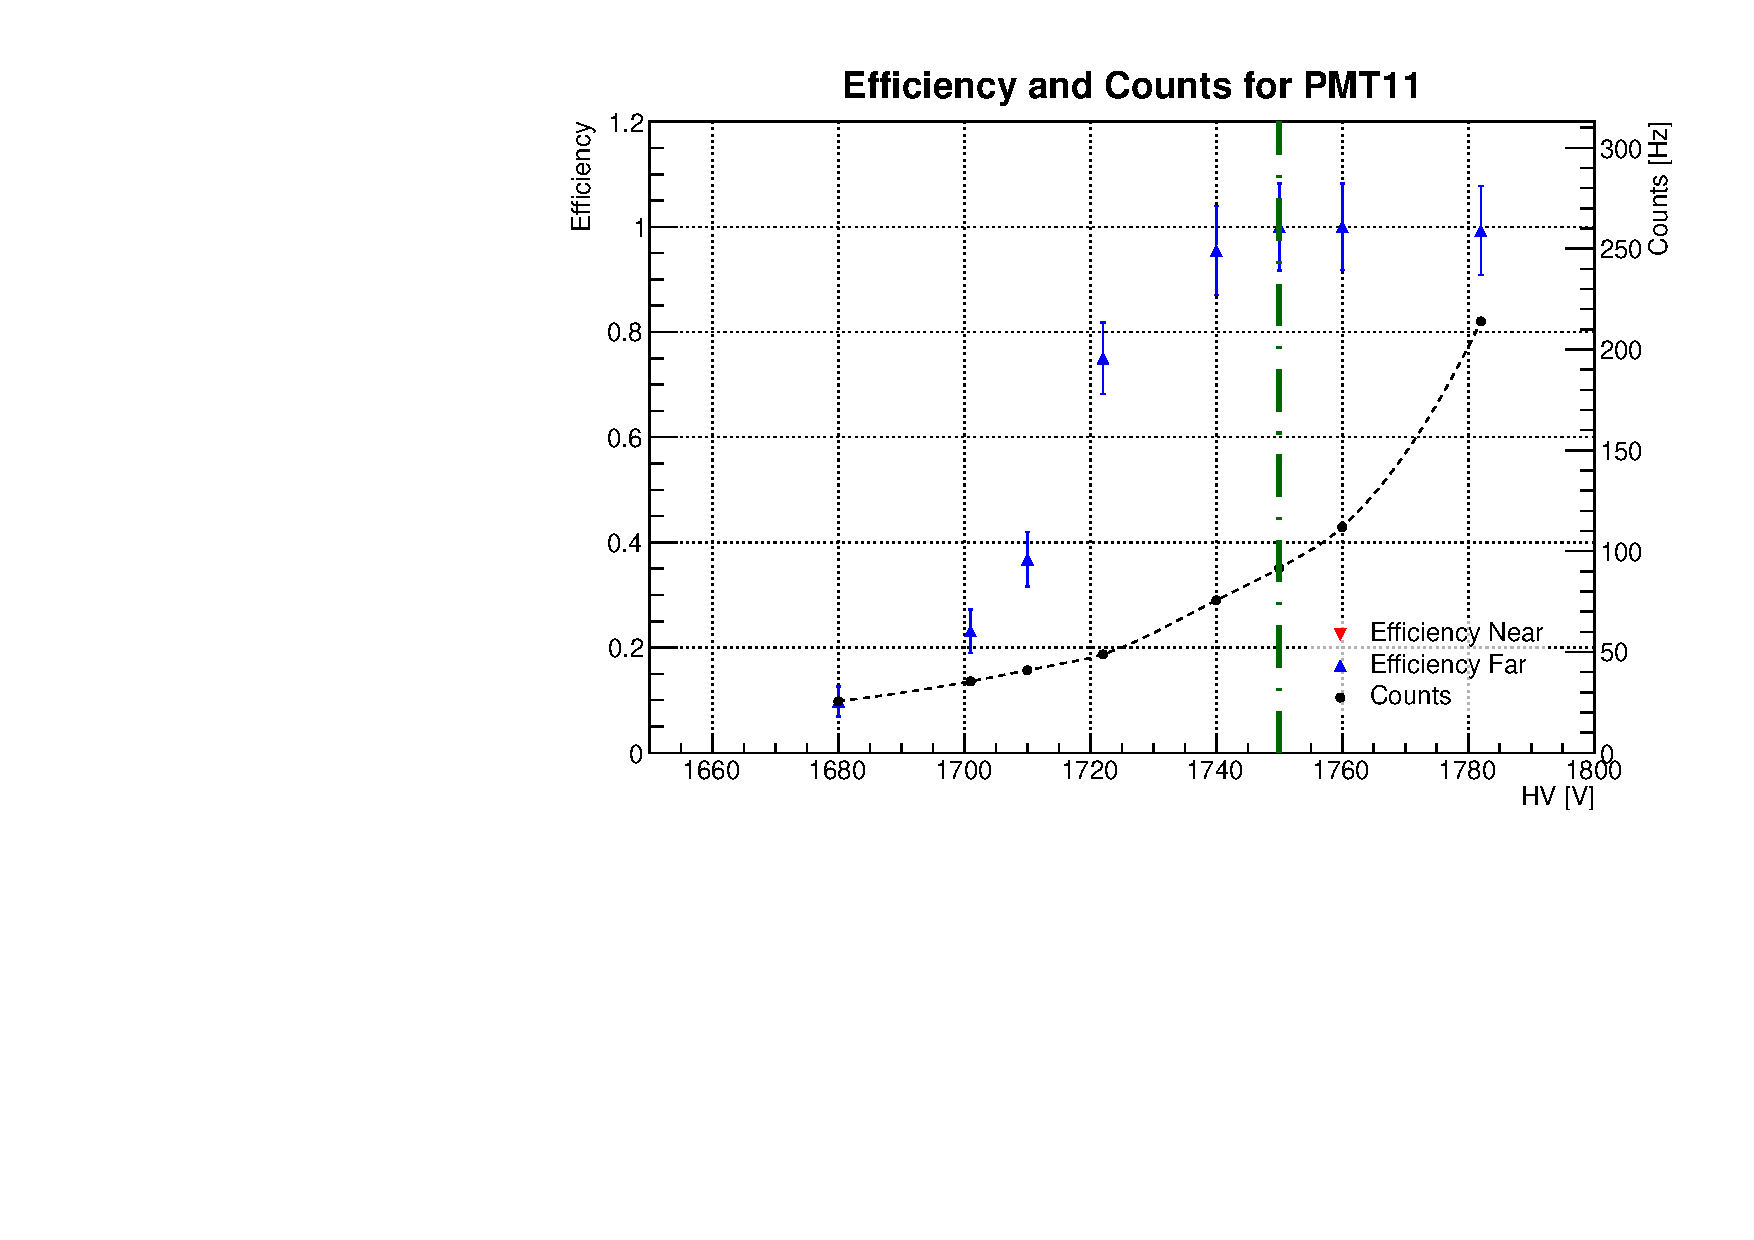
\includegraphics[scale=0.5]{img/eff11.pdf}}
%		\subfloat
%		{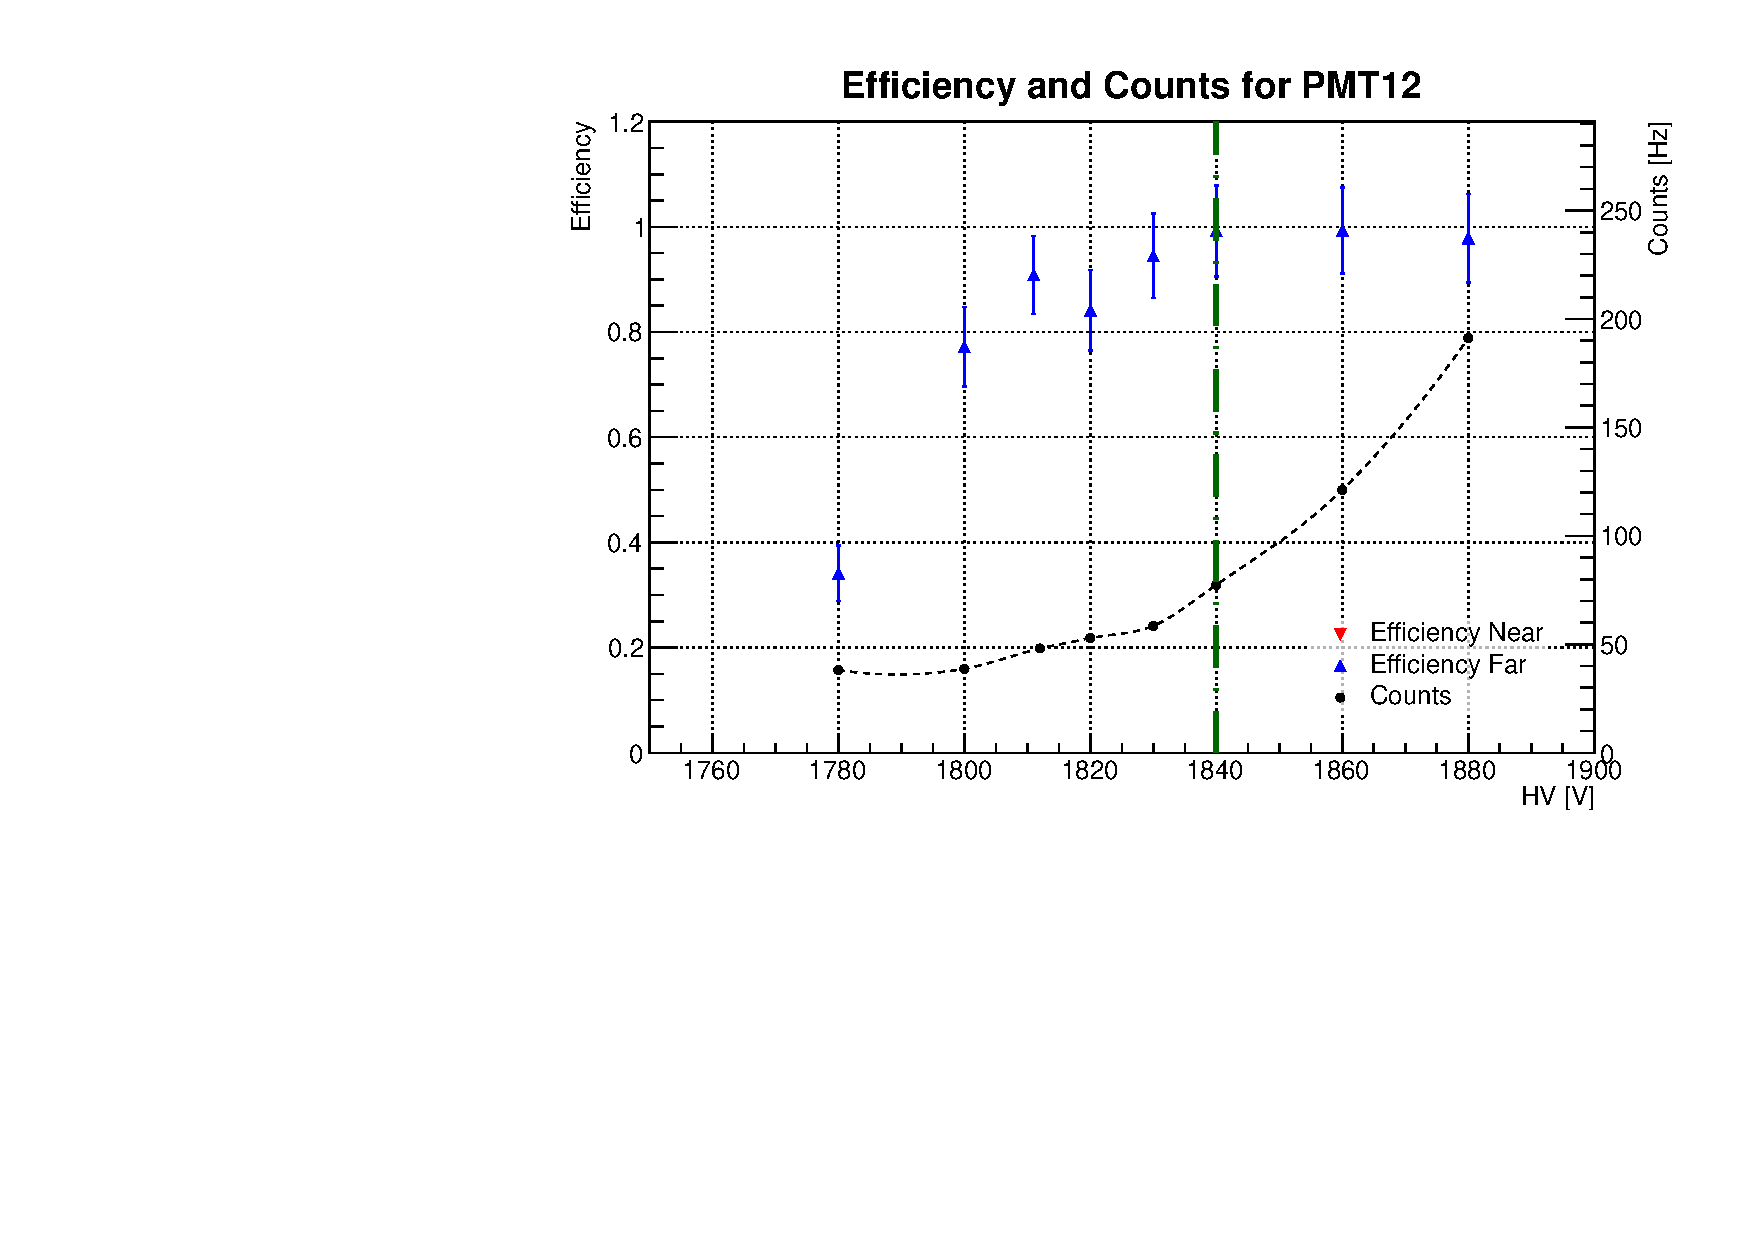
\includegraphics[scale=0.5]{img/eff12.pdf}}}
%\end{figure}
%\begin{figure}[h]
%	\centerline{
%		\subfloat
%		{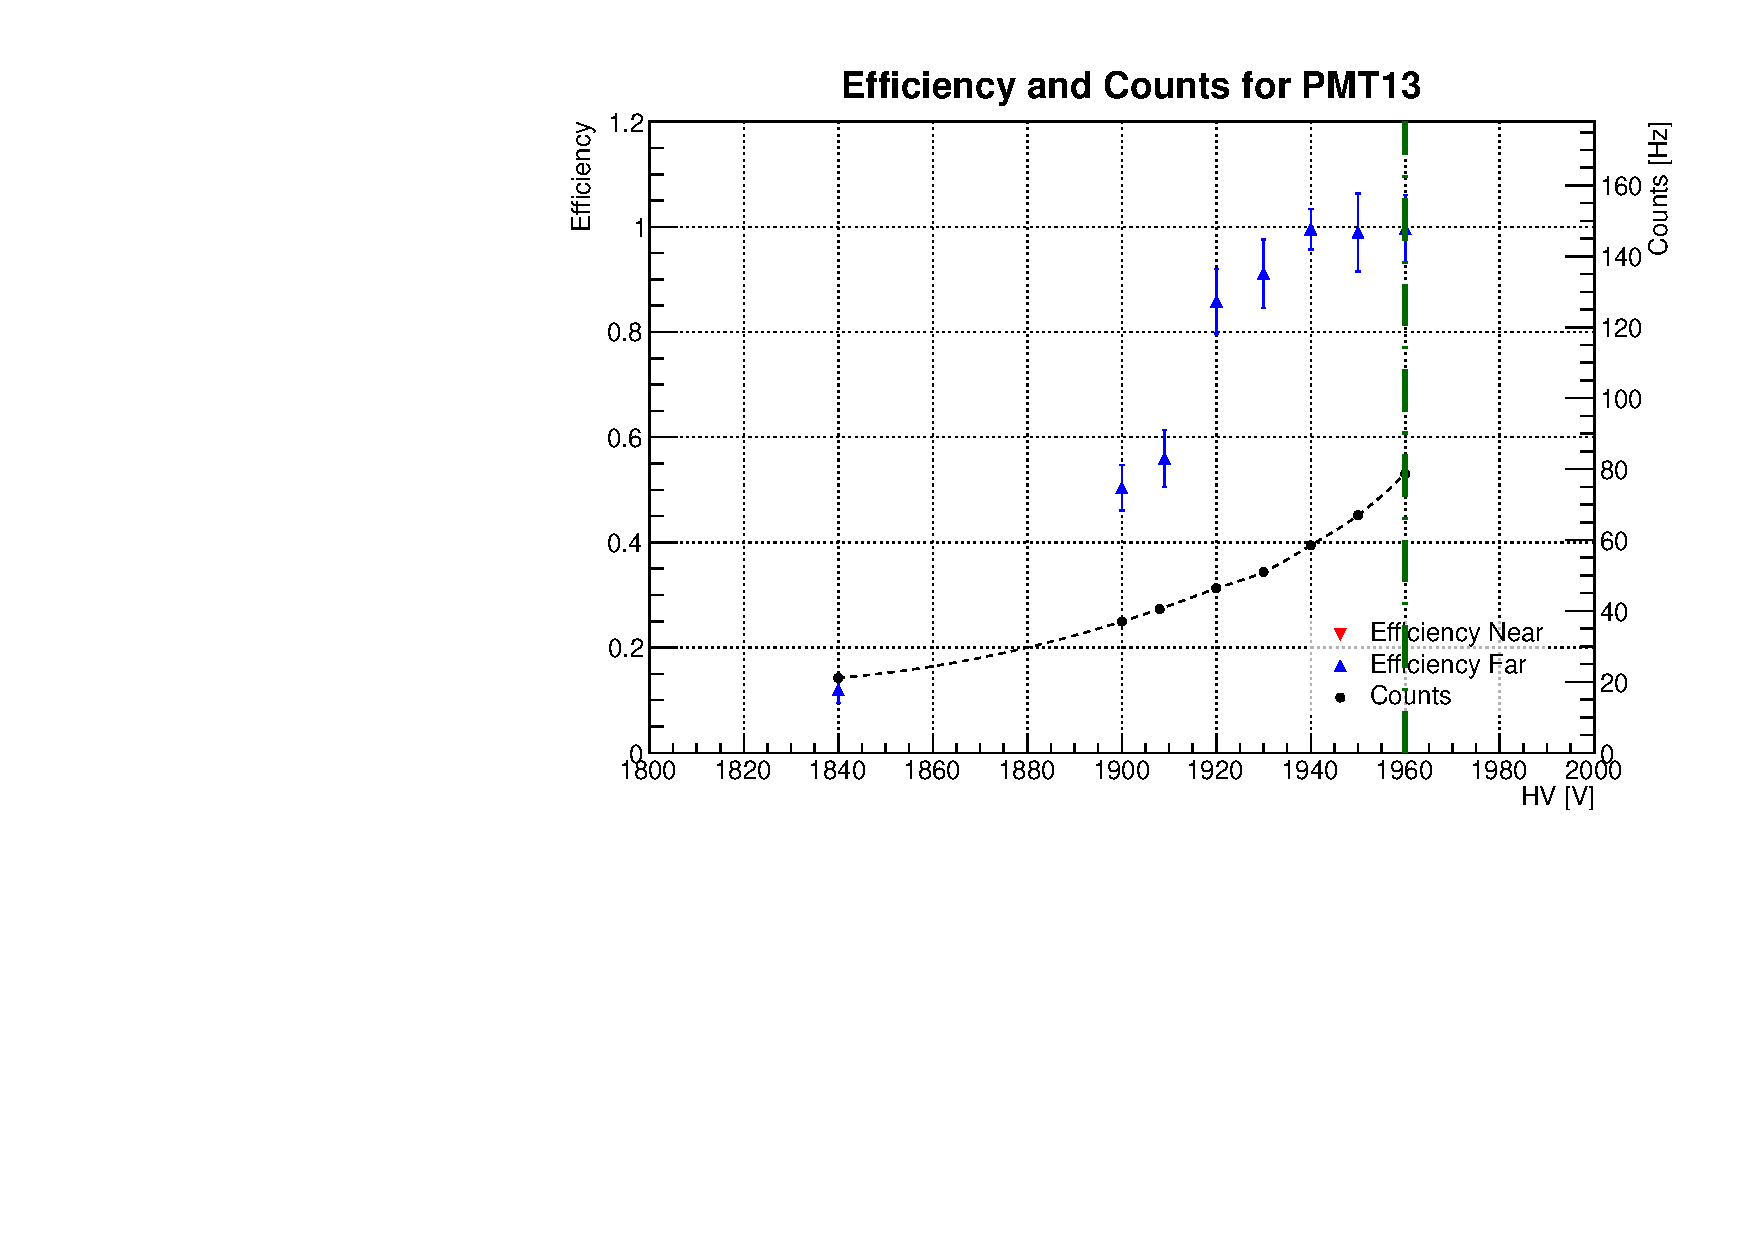
\includegraphics[scale=0.5]{img/eff13.pdf}}
%		\subfloat
%		{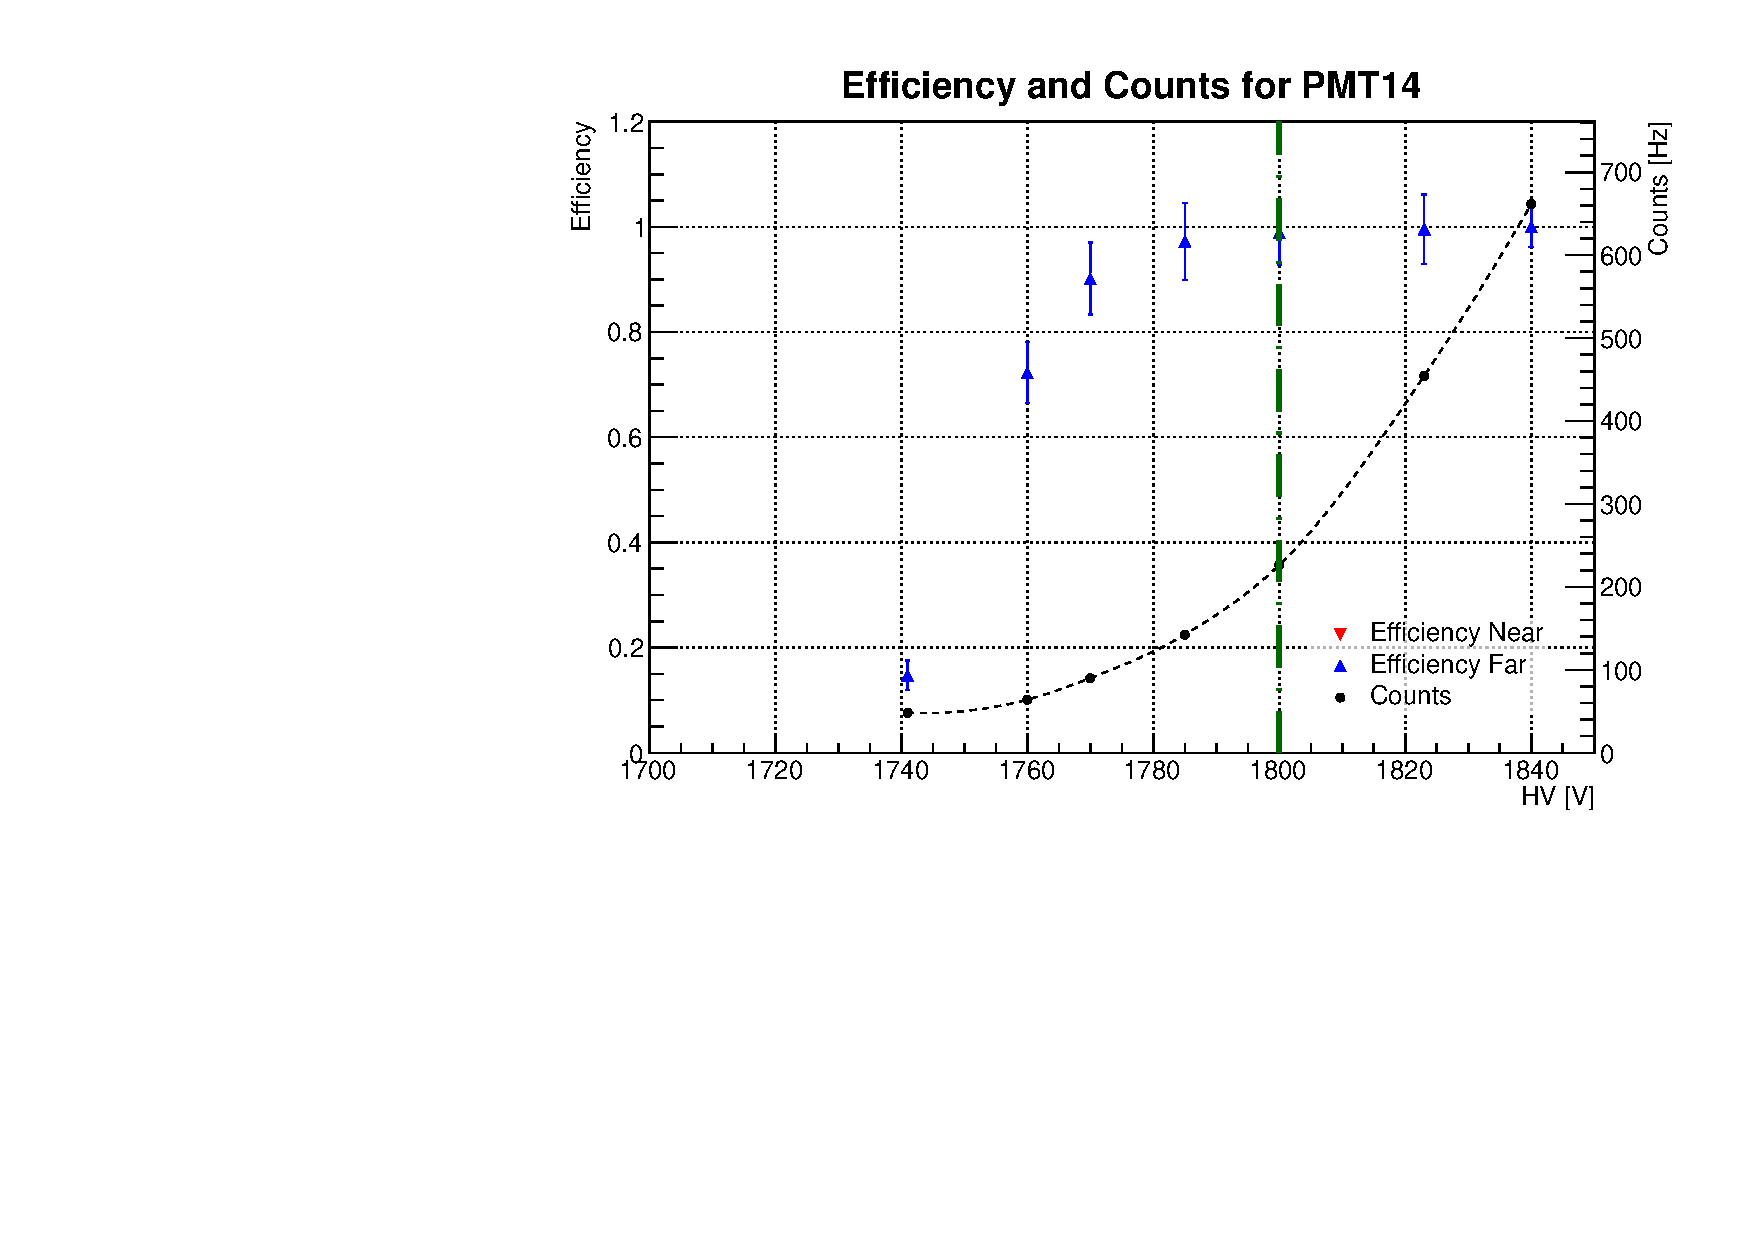
\includegraphics[scale=0.5]{img/eff14.pdf}}}
%\end{figure}

\end{document}
